\PassOptionsToPackage{dvipsnames}{xcolor}
\documentclass[10pt, xcolor={usenames, dvipsnames}]{beamer}

\usepackage[scale=2]{ccicons}
\usepackage{graphicx}
\usepackage{booktabs}
\usepackage{gensymb}
\usepackage{multimedia}
\usepackage{hyperref}
\usepackage{txfonts}
\usepackage{caption}
\usepackage{subcaption}
\usepackage{siunitx}
\usepackage{colortbl}
\usepackage{arydshln}

\usepackage[style=authoryear,backend=biber]{biblatex}
\renewcommand*{\nameyeardelim}{\addcomma\addspace}
\addbibresource{bib/abstract.bib}

% Beamer configuration
\usetheme[sectionpage=progressbar, numbering=counter, progressbar=frametitle]{metropolis}

\usepackage{xfp}
\usepackage{pgfplots}
\usepackage{pgfplotsthemetol}
\usepackage{tikz}
\usetikzlibrary{automata,positioning,arrows,decorations.pathmorphing,calc,patterns,decorations.markings,decorations.shapes,shapes.geometric,matrix}
\usepgfplotslibrary{groupplots,units}
\pgfplotsset{width=7cm,compat=1.18}

\tikzset{paint/.style={ draw=#1, fill=#1 },
         decorate with/.style=
{decorate,decoration={shape backgrounds,shape=#1,shape size=1mm,shape sep=.5cm}}}

% Plot style
\pgfplotsset{
    mplot/.style={
        width=.48\textwidth,
        height=.4\textheight,
        grid=major,
        grid style={dashed,gray!30},
        ylabel style={align=center, font=\bfseries\boldmath},
        xlabel style={align=center, font=\bfseries\boldmath},
        x tick label style={font=\bfseries\boldmath},
        y tick label style={font=\bfseries\boldmath},
        scaled ticks=false,
        label style={font=\footnotesize},
        xticklabel style={font=\footnotesize},
        yticklabel style={font=\footnotesize},
        every axis plot/.append style={solid,thick},
    },
}

% Progressbar
\setbeamercolor{progress bar}{
    fg=TolLightGreen,
    bg=TolLightGreen!50!black!30
}
\makeatletter
    \setlength{\metropolis@titleseparator@linewidth}{2pt}
    \setlength{\metropolis@progressonsectionpage@linewidth}{2pt}
    \setlength{\metropolis@progressinheadfoot@linewidth}{2pt}
\makeatother

% Footer
\setbeamertemplate{frame footer}{Quentin Brateau, ENSTA Bretagne}

% Block fill
\metroset{block=fill}

% Section pages numbering
\makeatletter
\renewcommand{\metropolis@enablesectionpage}{
  \AtBeginSection{
    \ifbeamer@inframe
      \sectionpage
    \else
      \frame[c,plain]{\sectionpage}
    \fi
  }
}
\metropolis@enablesectionpage
\makeatother

% Title
\title{CSI2023 - Torpedo-like AUV control in constrained environment}
\date{\today}
\author{Quentin Brateau}
\institute{ENSTA Bretagne}

\titlegraphic{
    \centering
    \begin{tabular}{lllll}
        \href{https://www.defense.gouv.fr/aid}{
\includegraphics[height=0.6cm]{imgs/logo_aid}} &
        \href{https://www.gdr-robotique.org/}{
\includegraphics[height=0.6cm]{imgs/logo_gdr}} &
        \href{https://www.ensta-bretagne.fr/fr/}{
\includegraphics[height=0.6cm]{imgs/logo_ensta}} &
        \href{https://labsticc.fr/fr}{
\includegraphics[height=0.6cm]{imgs/logo_labsticc}} &
        \href{https://www.ensta-bretagne.fr/robex/}{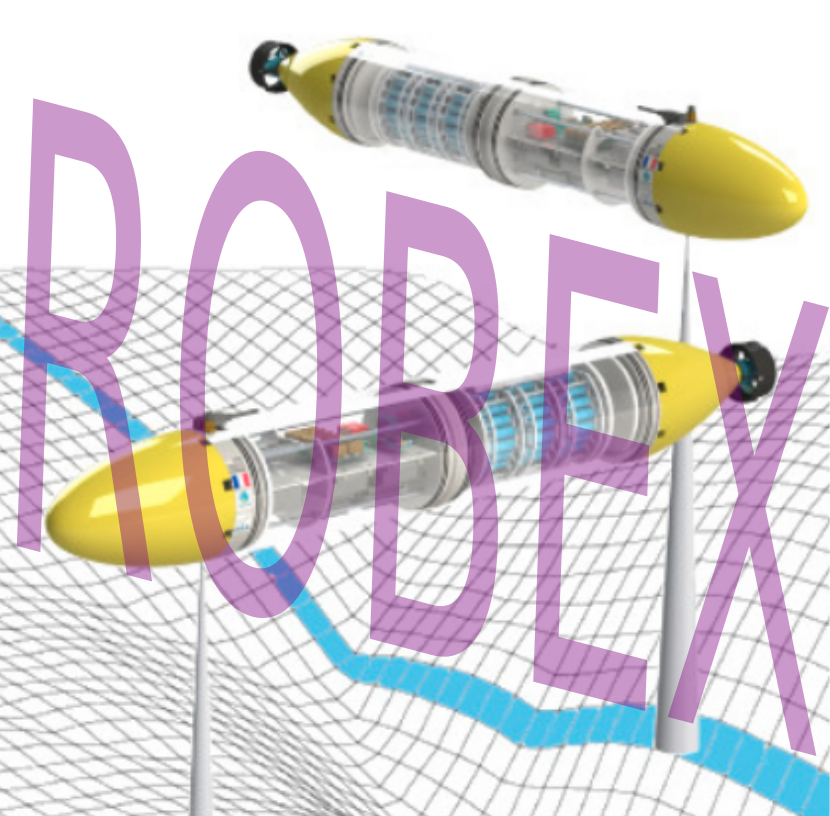
\includegraphics[height=0.6cm]{imgs/logo_robex}}
    \end{tabular}
}

\addtobeamertemplate{frametitle}{}{%
    \begin{tikzpicture}[remember picture,overlay]
    \node[anchor=north east,yshift=2pt] at (current page.north east) {
\includegraphics[height=0.85cm]{imgs/logo_ensta_aid}};
    \end{tikzpicture}
}

\begin{document}

    \maketitle

    \section{Context}

        \subsection{PhD presentation}

            \begin{frame}{PhD presentation}
                \centering
                \begin{minipage}[c]{0.58\textwidth}
                    \begin{block}{Research laboratory}
                        \vspace{0.2cm}
                        \begin{itemize}
                            \item ENSTA Bretagne, UMR 6285, Lab-STICC
                        \end{itemize}
                    \end{block}

                    \begin{block}{Supervisiors}
                        \begin{itemize}
                            \item Luc Jaulin
                            \item Fabrice Le Bars
                        \end{itemize}
                    \end{block}

                    \begin{block}{Funding}
                        \begin{itemize}
                            \item AID funding: Jean-Daniel Masson
                        \end{itemize}
                    \end{block}
                \end{minipage}
                \hfill
                \begin{minipage}[c]{0.4\textwidth}
                    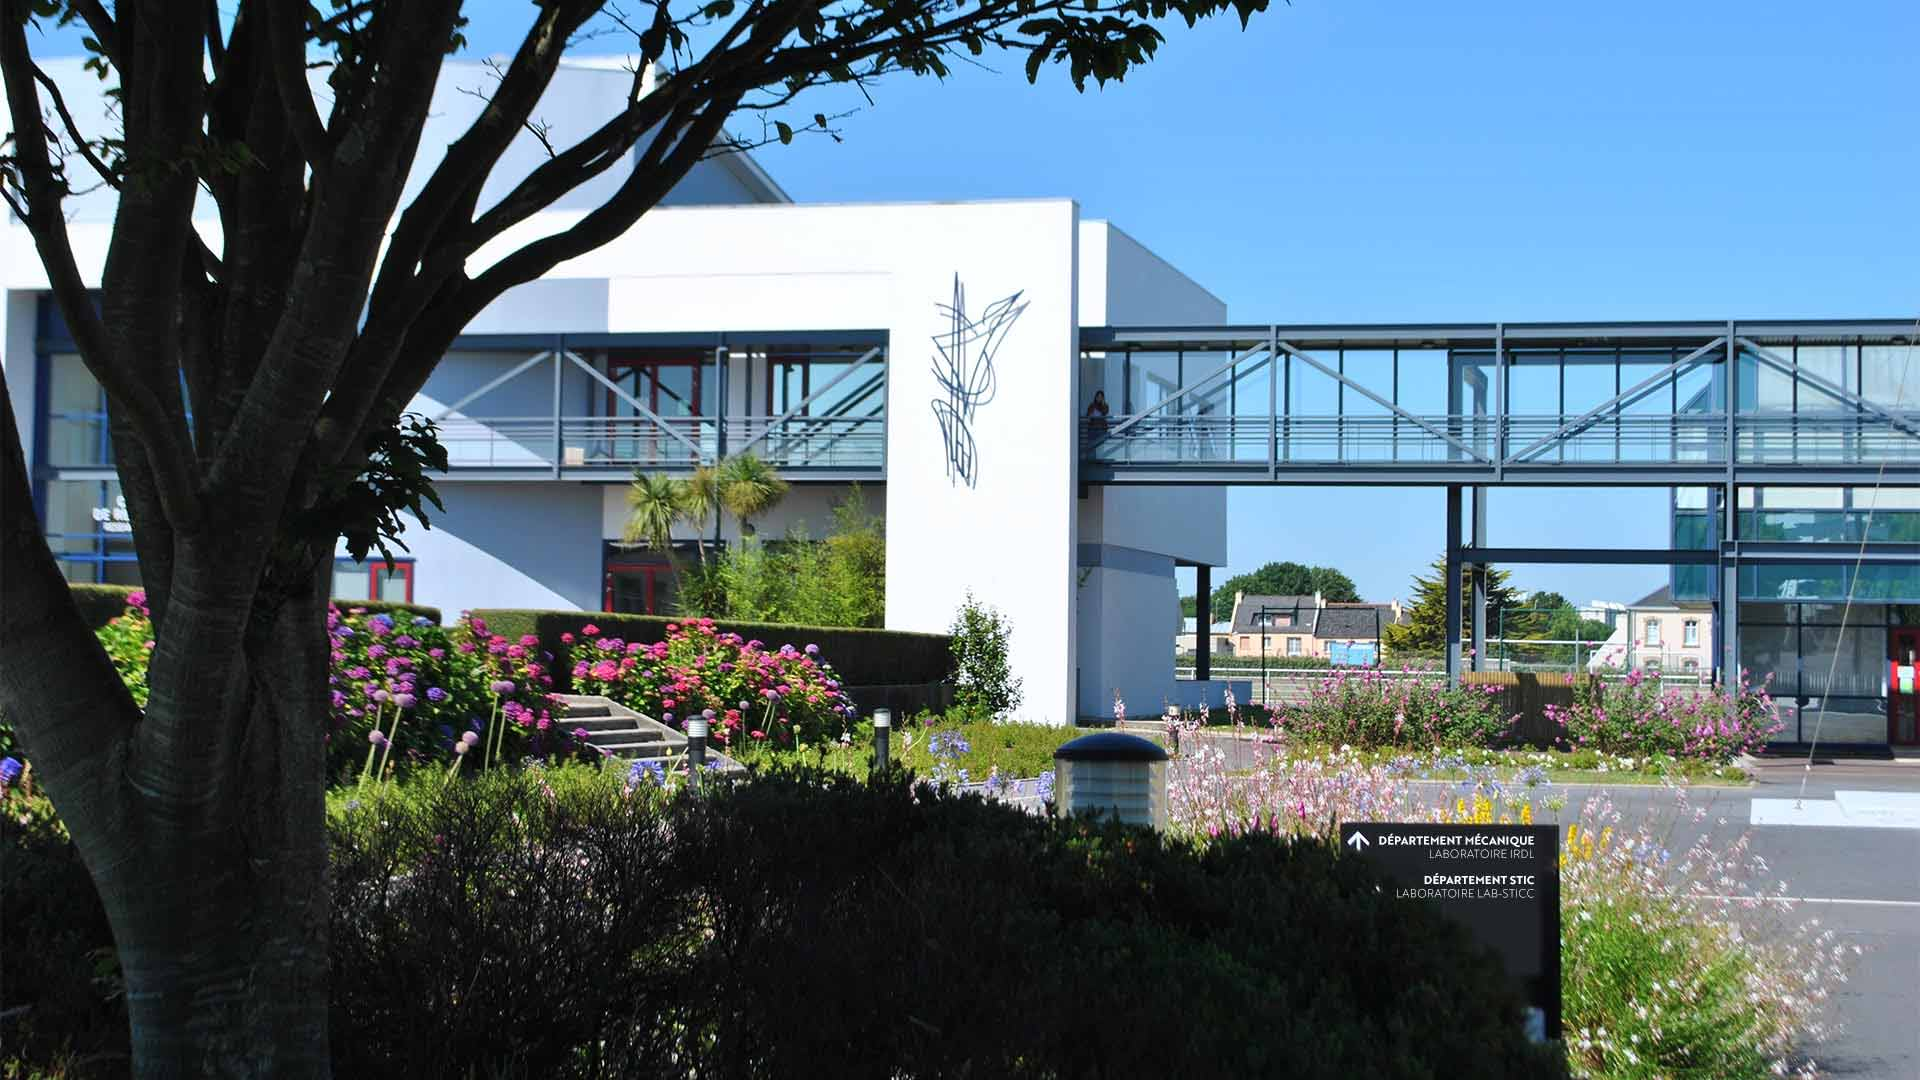
\includegraphics[height=0.7\textheight, trim={24cm 0 16cm 0}, clip]{imgs/ensta.jpg}
                \end{minipage}
            \end{frame}

        \subsection{PhD goal}

            \begin{frame}{PhD goal}
                \begin{minipage}[c]{0.55\textwidth}
                    \begin{block}{AUV}
                        \vspace{0.25cm}
                        \begin{itemize}
                            \item Control of torpedo-like AUV \\ 
                            \item Riptide's micro-uuv
                        \end{itemize}
                    \end{block}
                    \begin{block}{Environment}
                        \begin{itemize}
                            \item Constrained environment \\ 
                            \item Pool, harbor, ...
                        \end{itemize}
                    \end{block}
                    \begin{block}{Goals}
                        \begin{itemize}
                            \item Reactivity \\
                            \item Manoeuvrability
                        \end{itemize}
                    \end{block}
                \end{minipage}
                \hfill
                \begin{minipage}[c]{0.4\textwidth}
                    \begin{figure}[htb]
                        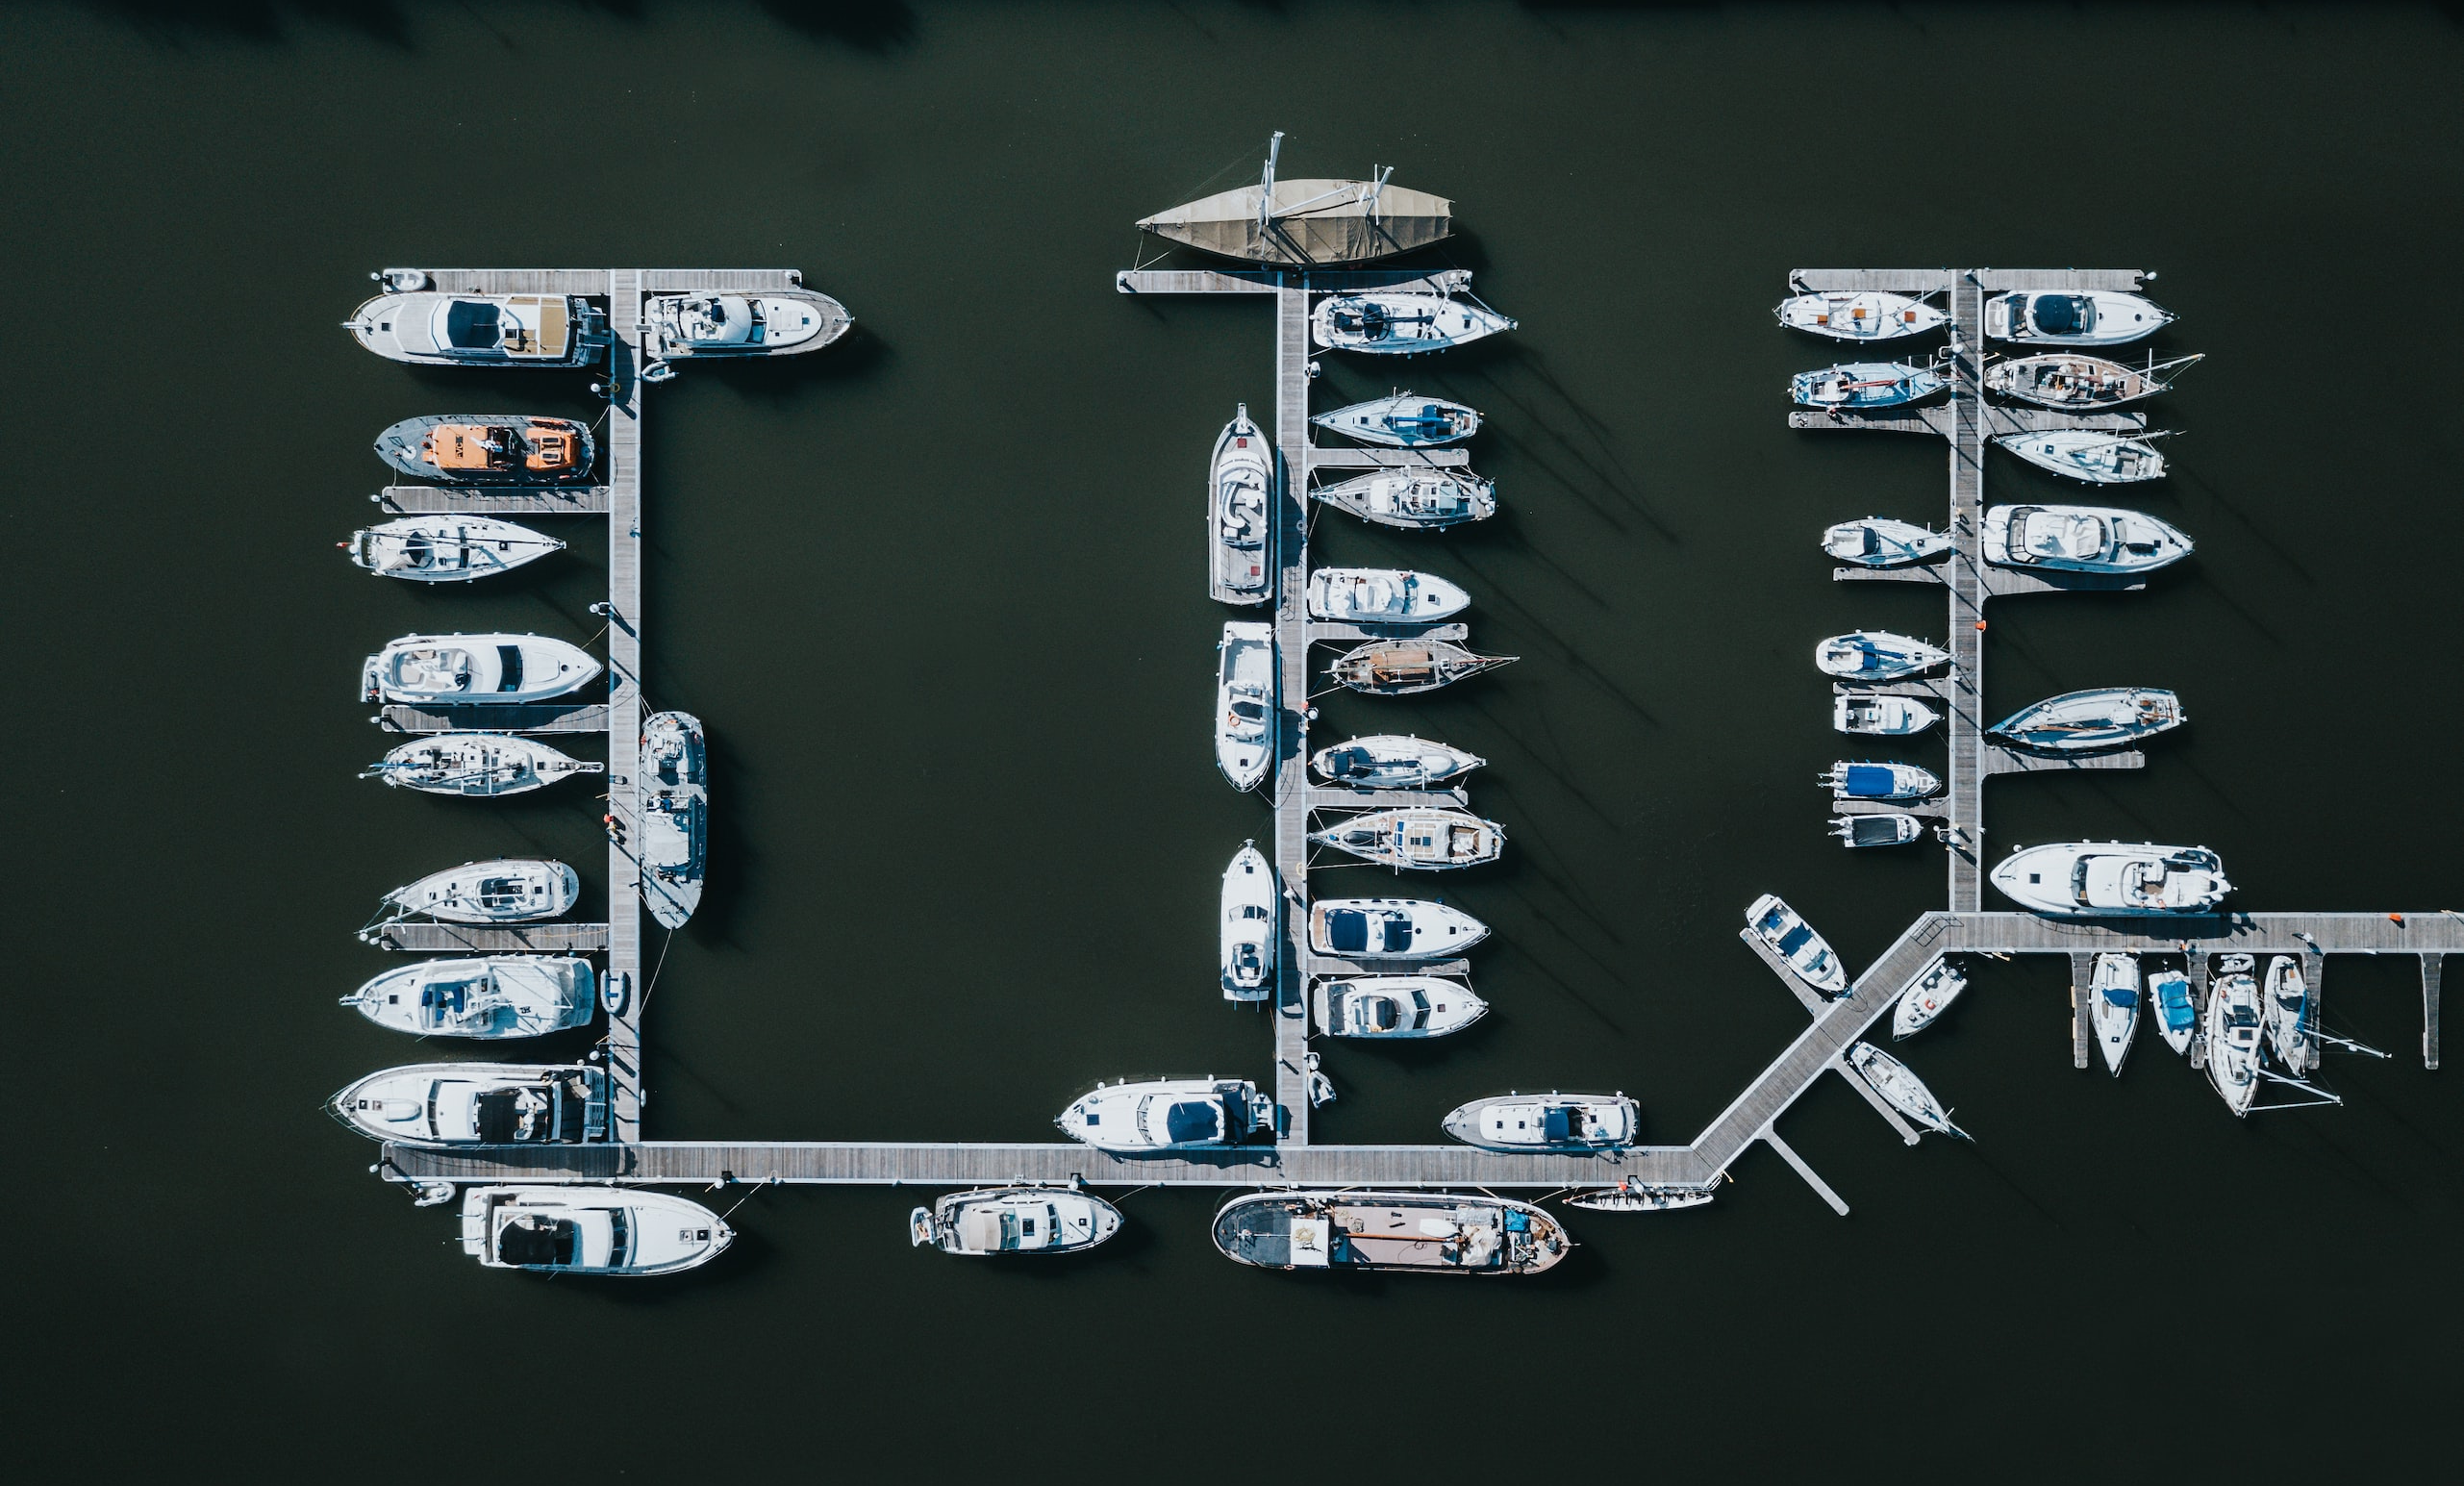
\includegraphics[width=\textwidth]{imgs/harbour.png}

                        \vspace{.1cm}

                        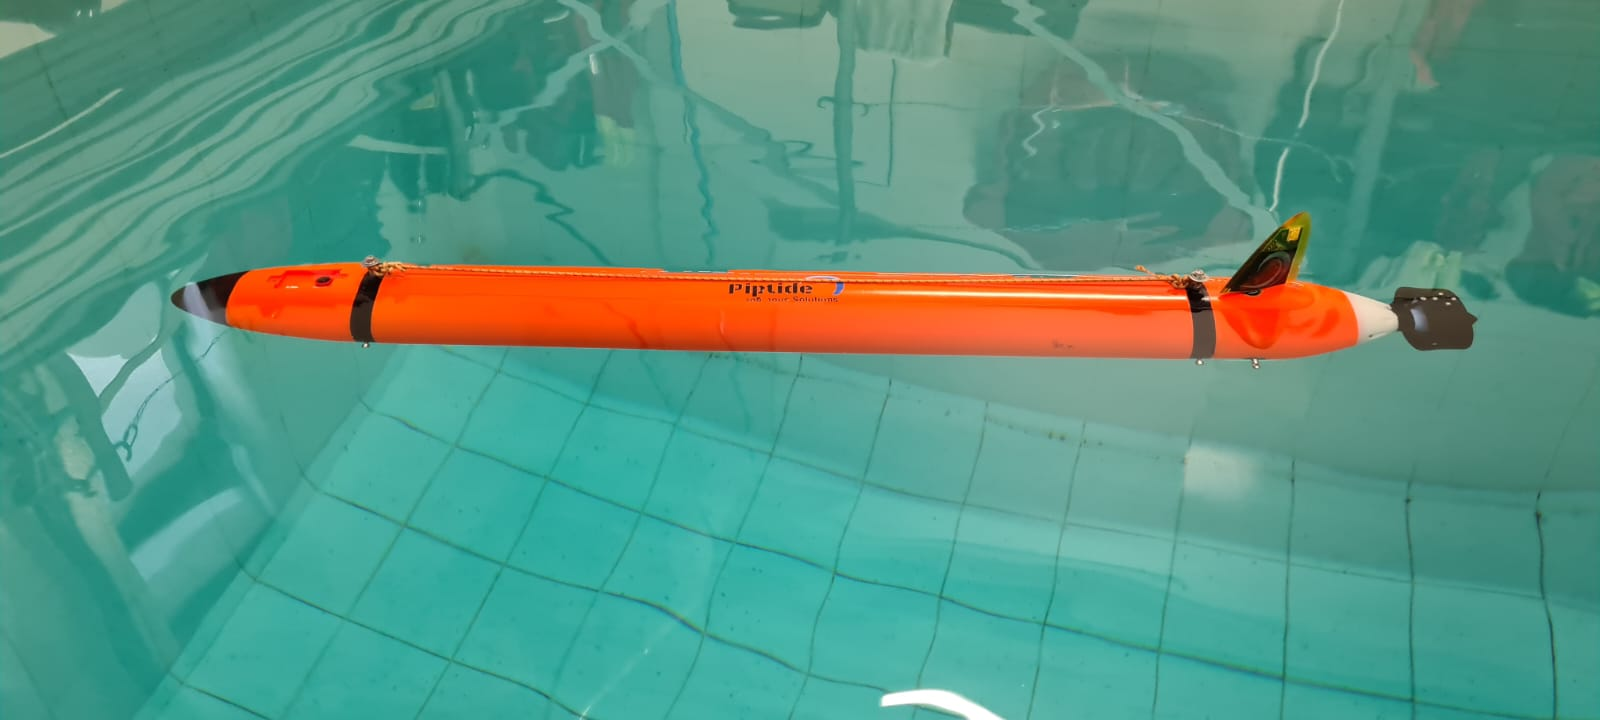
\includegraphics[width=\textwidth]{imgs/Riptide.jpeg}
                        \caption{Harbor and Riptide in the ENSTA Bretagne pool}
                    \end{figure}
                \end{minipage}
            \end{frame}

    \begin{frame}{Table of contents}
        \setbeamertemplate{section in toc}[sections numbered]
        \tableofcontents[hideallsubsections]
    \end{frame}

    \section{Riptide presentation}

        \begin{frame}{Torpedo Model}
            \begin{minipage}[t]{.48\textwidth}
                \begin{block}<+->{Controlled physical quantities}
                    \vspace{2.5mm}
                    \begin{itemize}
                        \item Linear acceleration $\mathbf{a_r}$
                        \item angular velocity $\mathbf{\omega_r}$
                    \end{itemize}
                \end{block}
                \begin{block}<+->{Robot's inputs}
                    \centering
                    Input vector of the system is $\mathbf{u} = (u_0, u_1, u_2, u_3)^T$, where:
                    \begin{itemize}
                        \item $u_0$: thruster velocity \\
                        \item $u_1, u_2, u_3$: fin angles
                    \end{itemize}
                \end{block}
            \end{minipage}
            \hfill
            \begin{minipage}[t]{.48\textwidth}
                \begin{block}<+->{Torpedo velocity}
                    \vspace{2.5mm}
                    \begin{equation}
                        \mathbf{v_r} = (v_r, 0, 0)^T
                    \end{equation}
                \end{block}
                \onslide<+->{
                    \begin{figure}
                        \centering
                        \includegraphics[width=.9\textwidth,trim={0 4cm 0 8cm},clip]{imgs/riptide_pontoon.jpg}
                        \caption{Riptide}
                    \end{figure}
                }
            \end{minipage}
        \end{frame}

        \begin{frame}{Operating systems}
            \begin{figure}
                \begin{subfigure}[c]{.5\textwidth}
                    \includegraphics[width=.95\textwidth]{imgs/simulation.png}
                    \subcaption{Riptide's simulator}
                \end{subfigure}%
                \begin{subfigure}[c]{.5\textwidth}
                    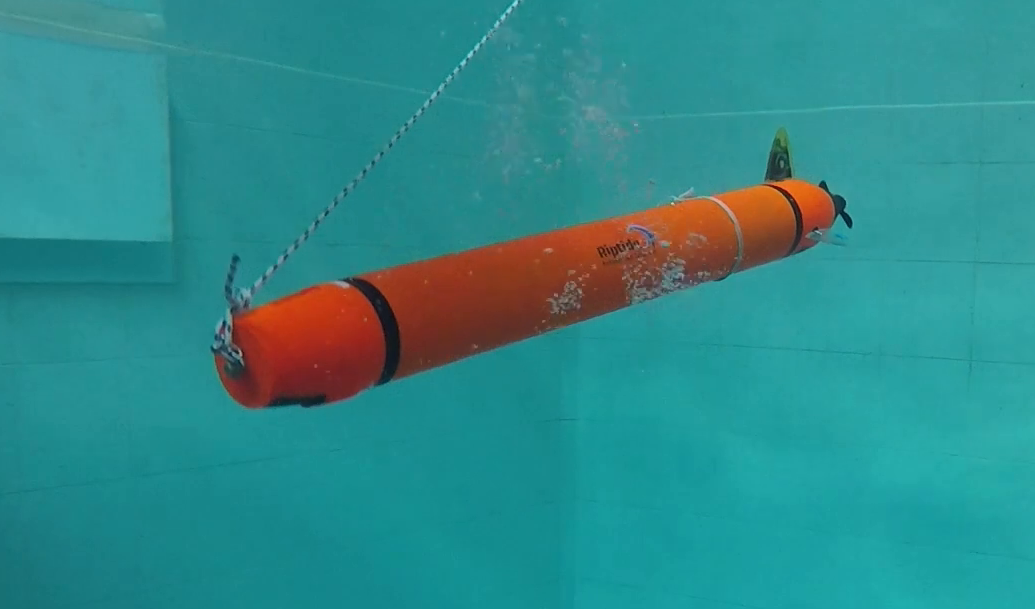
\includegraphics[width=.95\textwidth]{imgs/riptide.png}
                    \subcaption{Riptide robot}
                \end{subfigure}
                \caption{Riptide operating systems}
            \end{figure}
        \end{frame}

    \section{Attitude control for AUV}

        \begin{frame}{Attitude control for AUV}
            \begin{minipage}[c]{0.48\textwidth}
                \begin{block}{Log control}
                    \begin{itemize}
                        \vspace{0.25cm}
                        \item<2-> Simple control law
                        \item<3-> Complete attitude control
                        \item<4-> Fastest reorientation
                        \item<5-> Rigid control
                    \end{itemize}
                \end{block}
            \end{minipage}
            \hfill
            \begin{minipage}[c]{0.48\textwidth}
                \begin{block}{Orthogonal control}
                    \begin{itemize}
                        \vspace{0.25cm}
                        \item<2-> Simple control law
                        \item<3-> Partial attitude control
                        \item<4-> Fastest reorientation
                        \item<5-> Slack Control
                    \end{itemize}
                \end{block}
            \end{minipage}
        \end{frame}

        \subsection{Log Control}

            \begin{frame}{Log control - Illustration}
                \begin{figure}
                    \begin{subfigure}[t]{.5\textwidth}
                        \centering
                        \begin{tikzpicture}[
                            wavy/.style={->,>=latex,thick,decorate,
                            decoration={snake,amplitude=2mm,segment length=8mm,pre length=1mm, post length=1mm}}
                            ]
                            \shade[ball color = gray!40, opacity = 0.4] (0,0) circle (2cm);
                            \draw[thick] (0,0) circle (2cm);
                            \onslide<1->{
                                \begin{scope}
                                    \draw[thick] (-2,0) arc (180:360:2 and 0.6) coordinate[pos=0.3] (R3);
                                    \draw[dashed] (2,0) arc (0:180:2 and 0.6);
                                \end{scope}
                            }
                            \onslide<2->{
                                \coordinate (R1) at (0.8,1.3);
                                \draw[thick,red,->,>=latex] (0,0) -- node[midway,above left] {$\mathbf{u}$} (R1); 
                            }
                            \onslide<3->{
                                \draw[thick,RoyalBlue,->,>=latex] (0,0) -- node[midway,above] {$\mathbf{v}$} (R3);
                            }
                            \coordinate (R4) at (-0.8,1.3);
                            \onslide<4>{
                                \draw[wavy,ForestGreen] (R1) to[bend right=45] (R3);
                                \node[ForestGreen] at (R4) {$\mathbf{w}$};
                            }
                            \onslide<5>{
                                \path[thick,->,>=latex,RoyalPurple] (R1) edge[in=90,out=130] (R3);
                                \node[RoyalPurple] at (R4) {$\mathbf{w}$};
                            }
                        \end{tikzpicture}
                        \subcaption{Representation in $S^2$}
                    \end{subfigure}%
                    \begin{subfigure}[t]{.5\textwidth}
                        \centering
                        \begin{tikzpicture}[
                            wavy/.style={->,>=latex,thick,decorate,
                            decoration={snake,amplitude=2mm,segment length=8mm,pre length=1mm, post length=1mm}}
                            ]
                            \shade[ball color = gray!40, opacity = 0.4] (0,0) circle (2cm);
                            \draw[thick] (0,0) circle (2cm);
                            \onslide<1->{
                                \begin{scope}
                                    \draw[thick] (-2,0) arc (180:360:2 and 0.6) coordinate[pos=0.3] (R3);
                                    \draw[dashed] (2,0) arc (0:180:2 and 0.6);
                                \end{scope}
                            }
                            \onslide<3->{
                                \node[thick,RoyalBlue] at (R3) {$\bullet$} node[RoyalBlue] at (R3) [below] {$\mathbf{R_v}$};
                            }
                            \coordinate (R4) at (-0.8,1.3);
                            \onslide<4>{
                                \draw[wavy,ForestGreen,densely dotted] (R1) to[bend right=45] (R3);
                                \node[ForestGreen] at (R4) {$\mathbf{R_w}$};
                            }
                            \onslide<5->{
                                \path[thick,->,>=latex,RoyalPurple,densely dotted] (R1) edge[in=90,out=130] (R3);
                                \node[RoyalPurple] at (R4) {$\mathbf{R_w}$};
                            }
                            \onslide<2->{
                                \coordinate (R1) at (0.8,1.3);
                                \node[red] at (R1) {$\bullet$} node[red] at (R1) [below right] {$\mathbf{R_u}$};
                            }
                        \end{tikzpicture}
                        \caption{Representation in $SO(3)$}
                    \end{subfigure}
                    \caption{Log control}
                \end{figure}
            \end{frame}

            \begin{frame}{Log control - Formula}
                \centering
                \begin{minipage}{0.5\textwidth}
                    \begin{block}<+->{Rotation matrix}
                        \begin{equation}
                            \mathbf{\color{RoyalPurple}R_w} = \mathbf{\color{red}R_u}^T \cdot \mathbf{\color{RoyalBlue}R_v}
                        \end{equation}
                    \end{block}
                    \begin{block}<+->{Angular velocity w}
                        Link between $\mathbf{\color{RoyalPurple}w}$ and $\mathbf{\color{RoyalPurple}R_w}$.
                        \begin{align}
                            \onslide<+->{\mathbf{\color{RoyalPurple}R_w}^{\color{RubineRed}t} &= Exp~\mathbf{\color{RoyalPurple}w} \\}
                            \onslide<+->{\mathbf{\color{RoyalPurple}w} &= {\color{RubineRed}t} \cdot Log~\mathbf{\color{RoyalPurple}R_w} \\}
                            \notag
                        \end{align}
                        \vskip-1.5em
                    \end{block}
                \end{minipage}%
                \begin{minipage}{0.5\textwidth}
                    \centering
                    \begin{figure}
                        \begin{subfigure}[c]{\textwidth}
                            \centering
                            \begin{tikzpicture}
                                \shade[ball color = gray!40, opacity = 0.4] (0,0) circle (2cm);
                                \draw[thick] (0,0) circle (2cm);
                                \begin{scope}
                                    \draw[thick] (-2,0) arc (180:360:2 and 0.6) coordinate[pos=0.3] (R3);
                                    \draw[dashed] (2,0) arc (0:180:2 and 0.6);
                                \end{scope}
                                \coordinate (R1) at (0.8,1.3);
                                \coordinate (R4) at (-0.8,1.3);
                                \node[thick,RoyalBlue] at (R3) {$\bullet$} node[RoyalBlue] at (R3) [below] {$\mathbf{R_v}$};
                                \path[thick,->,>=latex,RoyalPurple,densely dotted] (R1) edge[in=90,out=130] (R3);
                                \node[RoyalPurple] at (R4) {$\mathbf{R_w}$};
                                \node[red] at (R1) {$\bullet$} node[red] at (R1) [below right] {$\mathbf{R_u}$};
                            \end{tikzpicture}
                            \caption{Representation in $SO(3)$}
                        \end{subfigure}
                        \caption{Log Control}
                    \end{figure}
                \end{minipage}%
            \end{frame}

            \begin{frame}{Log control - Extension}
                \begin{minipage}{.48\textwidth}
                    \begin{block}{2D Extension}
                        \vspace{.25cm}
                        \begin{itemize}[<+->]
                            \item $Log$ of a rotation matrix
                            \item Find sawtooth {\small $sawtooth(x) = 2 \cdot atan\left(tan\left(\frac{x}{2}\right)\right)$}
                        \end{itemize}
                    \end{block}
                    \begin{block}<+->{ND Extension}
                        \begin{itemize}[<+->]
                            \item Control of ND system
                        \end{itemize}
                    \end{block}
                \end{minipage}%
                \hfill
                \begin{minipage}{.5\textwidth}
                    \onslide<2->{
                        \begin{figure}
                            \centering
                            \begin{tikzpicture}
                                \begin{axis}[
                                        mplot, width=.95\textwidth, height=.5\textheight, name=sawtooth,
                                        xlabel=$\theta$, xmin=-6.28318, xmax=6.28318,
                                        xtick={-6.28318, -3.14159, 0, 3.14159, 6.28318},
                                        xticklabels={$-2\pi$, $-\pi$, 0, $\pi$, $2\pi$},
                                        ylabel=$Log(A(\theta))$, ymin=-4, ymax=4,
                                        ytick={-3.14159, 0, 3.14159},
                                        yticklabels={$-\pi$, 0, $\pi$},
                                        domain=-6.28318:6.28318, samples=100,
                                    ]
                                    \addplot[RoyalBlue] {2.*3.1415/180.*atan(tan(x*90/3.1415))};
                                \end{axis}
                            \end{tikzpicture}
                            \caption{$Log$ in $SO(2)$}
                        \end{figure}
                    }
                \end{minipage}
            \end{frame}

        \subsection{Orthogonal Control}

            \begin{frame}{Orthogonal control - Illustration}
                \begin{figure}
                    \begin{subfigure}[c]{.5\textwidth}
                        \centering
                        \begin{tikzpicture}
                            \shade[ball color = gray!40, opacity = 0.4] (0,0) circle (2cm);
                            \draw[thick] (0,0) circle (2cm);
                            \onslide<2->{
                                \coordinate (R1) at (0.8,1.3);
                                \draw[thick,red,->,>=latex] (0,0) -- node[midway,above left] {$\mathbf{u}$} (R1); 
                            }
                            \onslide<3->{
                                \coordinate (R2) at (-0.2,1.15);
                                \draw[thick,ForestGreen,->,>=latex] (0,0) -- node[midway,above left] {$\mathbf{v}$} (R2); 
                            }
                            \onslide<4->{
                                \begin{scope}[rotate around={-30:(0,0)}]
                                    \draw[thick] (-2,0) arc (180:360:2 and 0.6) coordinate[pos=0.36] (R3) coordinate[pos=0.61] (R4);
                                    \draw[dashed] (2,0) arc (0:180:2 and 0.6);
                                \end{scope}
                                \draw[thick,dotted] (R1) edge[in=30,out=175] (R2);
                                \draw[thick,RoyalBlue,->,>=latex] (0,0) -- node[midway,above] {$\mathbf{v_\bot}$} (R3);
                            }
                            \onslide<4>{
                                \draw[thick,dotted] (R2) edge[in=70,out=210] (R3);
                            }
                            \onslide<5->{
                                \path[thick,->,>=latex,RoyalPurple] (R2) edge[in=70,out=210] node[midway,above,left,RoyalPurple] {$\alpha$} (R3);
                                \draw[thick,RoyalPurple,->,>=latex] (0,0) -- node[midway,right] {$\mathbf{w}$} (R4);
                            }
                        \end{tikzpicture}
                        \subcaption{Representation in $S^2$}
                    \end{subfigure}%
                    \begin{subfigure}[c]{.5\textwidth}
                        \centering
                        \begin{tikzpicture}
                            \shade[ball color = gray!40, opacity = 0.4] (0,0) circle (2cm);
                            \draw[thick] (0,0) circle (2cm);
                            \onslide<2->{
                                \coordinate (R1) at (0.8,1.3);
                                \node[red] at (R1) {$\bullet$} node[red] at (R1) [below right] {$\mathbf{R_u}$};
                            }
                            \onslide<3->{
                                \coordinate (R2) at (-0.2,1.15);
                                \node[ForestGreen] at (R2) {$\bullet$} node[ForestGreen] at (R2) [above left] {$\mathbf{R_v}$};
                            }
                            \onslide<4->{
                                \begin{scope}[rotate around={-30:(0,0)}]
                                    \draw[thick] (-2,0) arc (180:360:2 and 0.6) coordinate[pos=0.36] (R3);
                                    \draw[dashed] (2,0) arc (0:180:2 and 0.6);
                                \end{scope}
                                \node[thick,RoyalBlue] at (R3) {$\bullet$} node[RoyalBlue] at (R3) [below left] {$\mathbf{R_{v_\bot}}$};
                            }
                            \onslide<5->{
                                \path[thick,->,>=latex,RoyalPurple,densely dotted] (R2) edge[in=70,out=210] node[midway, left] {$\mathbf{R_w}$} (R3);
                            }
                        \end{tikzpicture}
                        \subcaption{Representation in $SO(3)$}
                    \end{subfigure}
                    \caption{Orthogonal Control}
                \end{figure}
            \end{frame}

            \begin{frame}{Orthogonal Control - Determine $\mathbf{v_\bot}$}
                \begin{minipage}[c]{.4\textwidth}
                    \centering
                    \begin{figure}
                        \begin{tikzpicture}
                            \shade[ball color = gray!40, opacity = 0.4] (0,0) circle (2cm);
                            \draw[thick] (0,0) circle (2cm);
                            \coordinate (R1) at (0.8,1.3);
                            \draw[thick,red,->,>=latex] (0,0) -- node[midway,above left] {$\mathbf{u}$} (R1);
                            \begin{scope}[rotate around={-30:(0,0)}]
                                \draw[thick] (-2,0) arc (180:360:2 and 0.6) coordinate[pos=0.36] (R3);
                                \draw[dashed] (2,0) arc (0:180:2 and 0.6);
                            \end{scope}
    
                            \onslide<1-4> {
                                \coordinate (R2) at (-0.2,1.15);
                                \draw[thick,ForestGreen,->,>=latex] (0,0) -- node[midway,left]  {$\mathbf{v}$} (R2);
                            }
                            
                            \onslide<2> {
                                \coordinate (vu) at ($(0,0)!0.78!(R1)$);
                                \draw[thick,dotted] (vu) -- (R2);
                                \draw[thick,RoyalPurple,->,>=latex] (0,0) -- node[midway,right] {$\langle \mathbf{u}, \mathbf{v}\rangle \cdot \mathbf{u}$} (vu);
                            }
                            \onslide<3> {
                                \coordinate (vv) at ($(0,0)!0.72!(R3)$);
                                \draw[thick,RoyalPurple,->,>=latex] (vv) -- node[midway,left] {$\langle \mathbf{u}, \mathbf{v}\rangle \cdot \mathbf{u}$} (R2);
                                \draw[thick,RoyalBlue,->,>=latex] (0,0) -- node[midway,below right] {$\mathbf{v} - \langle \mathbf{u}, \mathbf{v}\rangle \cdot \mathbf{u}$} (vv);
                                }
                            \onslide<4> {
                                \draw[thick,RoyalBlue,->,>=latex] (0,0) -- node[midway,below right] {$\mathbf{v_\bot}$} (R3);
                            }
    
                            \onslide<5> {
                                \draw[thick,ForestGreen,->,>=latex] (0,0) -- node[midway,right] {$\mathbf{v}$} (R1);
                            }
                        \end{tikzpicture}
                        \caption{Representation in $S^2$}
                    \end{figure}
                \end{minipage}%
                \hfill
                \begin{minipage}[c]{.55\textwidth}
                    \vfill
                    \begin{block}{Determine $\mathbf{v_\bot}$}
                        \begin{equation}
                            \mathbf{\color{RoyalBlue}{v_\bot}} = \frac{\mathbf{\color{ForestGreen}{v}} - \langle \mathbf{\color{red}{u}}, \mathbf{\color{ForestGreen}{v}}\rangle \cdot \mathbf{\color{red}{u}}}{||\mathbf{\color{ForestGreen}{v}} - \langle \mathbf{\color{red}{u}}, \mathbf{\color{ForestGreen}{v}}\rangle \cdot \mathbf{\color{red}{u}}||}
                        \end{equation}
                    \end{block}
                    \begin{block}<5->{Limitation}
                        Physical singularity when $\mathbf{\color{red}{u}} = \mathbf{\color{ForestGreen}{v}}$, as $\mathbf{\color{RoyalBlue}{v_\bot}}$ is undefined
                    \end{block}
                    \vfill
                \end{minipage}
            \end{frame}

            \begin{frame}{Orthogonal Control - Determine $\mathbf{\omega}$}
                \begin{minipage}[c]{.4\textwidth}
                    \centering
                    \begin{figure}
                        \begin{tikzpicture}
                            \shade[ball color = gray!40, opacity = 0.4] (0,0) circle (2cm);
                            \draw[thick] (0,0) circle (2cm);
                            \coordinate (R1) at (0.8,1.3);
                            \draw[thick,red,->,>=latex] (0,0) -- node[midway,above left] {$\mathbf{u}$} (R1);
                            \draw[thick,RoyalBlue,->,>=latex] (0,0) -- node[midway,above] {$\mathbf{v_\bot}$} (R3);
                            \begin{scope}[rotate around={-30:(0,0)}]
                                \draw[thick] (-2,0) arc (180:360:2 and 0.6) coordinate[pos=0.36] (R3) coordinate[pos=0.61] (R4);
                                \draw[dashed] (2,0) arc (0:180:2 and 0.6)  coordinate[pos=0.36] (R5);
                            \end{scope}
                            
                            \onslide<1>{
                                \coordinate (R2) at (-0.2,1.15);
                                \draw[thick,ForestGreen,->,>=latex] (0,0) -- node[midway,above left] {$\mathbf{v}$} (R2); 
                                \draw[thick,dotted] (R1) edge[in=30,out=175] (R2);
                                \draw[thick,dotted] (R2) edge[in=70,out=210] (R3);
                            }
    
                            \onslide<2>{
                                \draw[thick,ForestGreen,->,>=latex] (0,0) -- node[midway,below right] {$\mathbf{v}$} (R3);
                            }
    
                            \onslide<3>{
                                \draw[thick,ForestGreen,->,>=latex] (0,0) -- node[midway,below right] {$\mathbf{v}$} (R5);
                            }
                        \end{tikzpicture}
                        \caption{Representation in $S^2$}
                    \end{figure}
                \end{minipage}
                \hfill
                \begin{minipage}[c]{.55\textwidth}
                    \vfill
                    \begin{block}{Rotation matrix}
                        \begin{equation}
                            \begin{array}{rcl}
                                \mathbf{K}_{\mathbf{\color{ForestGreen}{v}}}^{\mathbf{\color{RoyalBlue}{v_\bot}}} & = & \mathbf{\color{RoyalBlue}{v_\bot}} \mathbf{\color{ForestGreen}{v}}^T - \mathbf{\color{ForestGreen}{v}}\mathbf{\color{RoyalBlue}{v_\bot}}^T \\
                                \mathbf{R}_{\mathbf{\color{ForestGreen}{v}}}^{\mathbf{\color{RoyalBlue}{v_\bot}}} & = & \mathbf{I_3} + \mathbf{K}_{\mathbf{\color{ForestGreen}{v}}}^{\mathbf{\color{RoyalBlue}{v_\bot}}} + \frac{1}{1 + \color<3>{red}{\langle \mathbf{\color<-2>{ForestGreen}{v}}, \mathbf{\color<-2>{RoyalBlue}{v_\bot}}\rangle}} (\mathbf{K}_{\mathbf{\color{ForestGreen}{v}}}^{\mathbf{\color{RoyalBlue}{v_\bot}}})^2 \\
                            \end{array}
                        \end{equation}
                    \end{block}
                    \begin{block}<2->{No singularities}
                        \vspace{.2cm}
                        \begin{itemize}
                            \item If $\mathbf{\color{ForestGreen}{v}} = \mathbf{\color{RoyalBlue}{v_\bot}}$, $\mathbf{K}_{\mathbf{\color{ForestGreen}{v}}}^{\mathbf{\color{RoyalBlue}{v_\bot}}}=\mathbf{O_3}$ and $\mathbf{R_{{\color{ForestGreen}{v}}}^{{\color{RoyalBlue}{v_\bot}}}} = \mathbf{I_3}$ 
                            \item<3> Singularity when $\langle\mathbf{\color{ForestGreen}{v}}, \mathbf{\color{RoyalBlue}{v_\bot}}\rangle = -1$
                        \end{itemize}
                    \end{block}
                    \vfill
                \end{minipage}
            \end{frame}

        \subsection{Approaches comparison}

            \begin{frame}{Approaches comparison}
                \begin{minipage}[t]{0.48\textwidth}
                    \centering
                    \textbf{\large Classical control}
                    \begin{block}<2->{Strengths}
                        \begin{itemize}
                            \item Fully controlled attitude
                        \end{itemize}
                    \end{block}
                    \begin{block}<3->{Weaknesses}
                        \begin{itemize}
                            \item Complete knowledge of $\mathbf{R}$
                            \item Complete attitude setpoint
                            \item Slower reorientation
                        \end{itemize}
                    \end{block}
                \end{minipage}
                \hfill
                \begin{minipage}[t]{0.48\textwidth}
                    \centering
                    \textbf{\large Orthogonal control}
                    \begin{block}<2->{Strengths}
                        \begin{itemize}
                            \item Partial knowledge of $\mathbf{R}$
                            \item Partial attitude control
                            \item Quickest reorientation
                            \item Controllable remaining attitude
                        \end{itemize}
                    \end{block}
                    \begin{block}<3->{Weaknesses}
                        \begin{itemize}
                            \item Uncontrolled direction
                        \end{itemize}
                    \end{block}
                \end{minipage}
            \end{frame}
    
    \section{Trials}

        \subsection{Guerlédan}

            \begin{frame}{Trials}
                \begin{minipage}[c]{.55\textwidth}
                    \begin{block}<+->{2023 - Week 6}
                        \vspace{2.5mm}
                        \begin{itemize}
                            \item Riptide first trial
                            \item Riptide controller
                        \end{itemize}
                    \end{block}
                    \begin{block}<+->{2023 - Week 8}
                        \begin{itemize}
                            \item Riptide hardware fix
                            \item Depth controller
                        \end{itemize}
                    \end{block}
                    \begin{block}<+->{2023 - Week 21}
                        \begin{itemize}
                            \item Riptide hardware test
                            \item Log controller
                        \end{itemize}
                    \end{block}
                \end{minipage}%
                \hfill
                \begin{minipage}[c]{.43\textwidth}
                    \centering
                    \begin{figure}
                        \centering
                        \begin{subfigure}[t]{.9\textwidth}
                            \centering
                            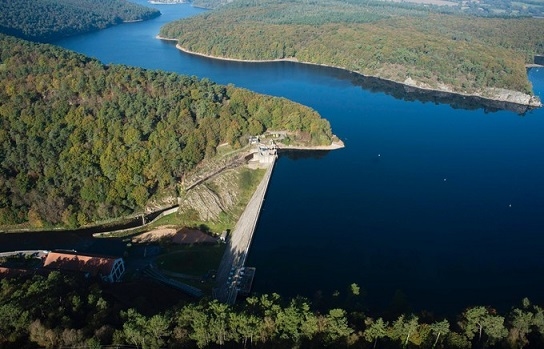
\includegraphics[width=\textwidth,trim={0 1cm 0 0.8cm},clip]{imgs/lac-de-guerledan.jpg}
                            \subcaption{Guerlédan's dam\footnote[frame]{\url{https://www.saint-aignan56.fr/tourisme/lac-de-guerledan/}}}
                        \end{subfigure}
                        \hfill
                        \begin{subfigure}[t]{.9\textwidth}
                            \centering
                            \includegraphics[width=\textwidth,trim={0 16cm 0 20cm},clip]{imgs/riptide_pontoon_2.jpg}
                            \subcaption{Riptide on pontoon}
                        \end{subfigure}
                        \caption{Guerlédan trials}
                    \end{figure}
                \end{minipage}
            \end{frame}

        \subsection{Depth controller trial}

            \begin{frame}{Depth Controller - Bloc diagram}
                \centering
                \begin{figure}
                    \begin{tikzpicture}[
                        input/.style={->,>=latex,thick,decorate,
                        decoration={snake,amplitude=.4mm,segment length=2mm,post length=2mm}},
                        block/.style={draw,font=\small,thick,
                            minimum width={2cm},minimum height={1.5cm}}]

                        \onslide<1-> \node[block,rectangle,align=center] (n3) {AUV};

                        \onslide<2->{
                            \node[block,circle,left=of n3] (n2) {Controller};
                            \coordinate (twist) at (n2.west);
                            \foreach \i/\a/\s in {0/37.5/-2.4,1/12.5/-3,2/-12.5/-3,3/-37.5/-2.5} {
                                \draw[thick,->,>=latex,Dandelion] (n2.\a) to node[near end,xshift=\s*1mm,yshift=1.5mm] {$u_\i$} ([yshift=0.6cm -\i * 0.4 cm]n3.west);
                            }
                        }

                        \onslide<3->{
                            \node[block,circle,left=of n2,align=center] (n1) {Depth\\controller};
                            \draw[thick,->,>=latex,RoyalBlue] (n1) to node[midway,above] {$\mathbf{v}$} node[midway,below] {$\mathbf{w}$} (twist);
                        }

                        \onslide<4->{
                            \coordinate(t) at ([shift=({145:2 cm})]n1);
                            \draw[input,ForestGreen] (t) -- node[midway,below left,ForestGreen] {$\mathbf{d}$} (n1.145);
                        }

                        \onslide<5->{
                            \node[yshift=-0.8cm,RoyalPurple] (f) at (n2.south) {$\mathbf{d}$, $\mathbf{pitch}$};
                            \draw[thick,RoyalPurple,->,>=latex] (n3.south) |- ($(f)+(0,0.3)$) -| (n1.south);
                        }
                    \end{tikzpicture}
                    \caption{Depth controller - Closed-loop block diagram}
                \end{figure}
            \end{frame}

            \begin{frame}{Mission description}
                \sisetup{input-digits = 0123456789\infty}
                \centering
                \begin{minipage}[c]{0.4\textwidth}
                    \centering
                    \begin{table}
                        \begin{tabular}[t]{ccc}
                            \toprule
                            State & Depth & Duration \\
                            \midrule
                            $q_0$ & $\qty{0}{\m}$ & $\qty{\infty}{\s}$ \\
                            % \AC{red} \hdashline[.6pt/1.2pt] \EAC
                            $q_1$ & $\qty{2}{\m}$ & $\qty{10}{\s}$ \\
                            $q_2$ & $\qty{1}{\m}$ & $\qty{10}{\s}$ \\
                            $q_3$ & $\qty{2}{\m}$ & $\qty{10}{\s}$ \\
                            \bottomrule
                        \end{tabular}
                        \caption{States description}
                    \end{table}
                \end{minipage}
                \hfill
                \begin{minipage}[c]{0.55\textwidth}
                    \begin{figure}[\textwidth]
                        \centering
                        \begin{tikzpicture}[node distance=2cm,on grid,auto]
                            \node[state, initial, accepting] (q0) {$q_0$};
                            \node[state, above right of=q0] (q1) {$q_1$};
                            \node[state, below right of=q0] (q3) {$q_3$};
                            \node[state, below right of=q1] (q2) {$q_2$};
                            
                            \draw[->,>=latex]
                                (q0) edge node[midway, above left] {\color{RubineRed}{trigger}} (q1)
                                (q1) edge node[midway, above right] {$d=\qty{10}{\s}$} (q2)
                                (q2) edge node[midway, below right] {$d=\qty{10}{\s}$} (q3)
                                (q3) edge node[midway, below left] {$d=\qty{10}{\s}$} (q0);
                        \end{tikzpicture}
                        \caption{FSM of the mission}
                    \end{figure}
                \end{minipage}
            \end{frame}

            \begin{frame}{Simulation}
                \centering
                \begin{minipage}[c]{0.95\textwidth}
                    \begin{figure}
                        \href{run:simulation.mkv?autostart&loop}{\includegraphics[width=\textwidth]{build/imgs/videos/simulation}}
                        \caption{Mission simulation}
                    \end{figure}
                \end{minipage}
            \end{frame}

            \begin{frame}{Simulation Data}
                \centering
                \begin{figure}
                    \centering
                    \begin{tikzpicture}
                        \begin{axis}[
                                mplot,
                                name=depth,
                                xlabel=Time,
                                ylabel=Depth,
                                x unit=\si{\s},
                                y unit=\si{\m},
                            ]
                            \addplot[RoyalBlue] table [x expr={\fpeval{\thisrow{pressure_stamp} - 1681203552.}}, y=depth, col sep=comma] {data/simulation.csv};
                        \end{axis}

                        \begin{axis}[
                                mplot,
                                name=fins,
                                at=(depth.right of north east), anchor=left of north west,
                                xshift=.25cm,
                                xlabel=Time,
                                ylabel=Fin angle,
                                x unit=\si{\s},
                                y unit=\si{\radian},
                            ]
                            \addplot[Dandelion] table [x expr={\fpeval{\thisrow{time} - 1681203552.}}, y=p_fin, col sep=comma] {data/simulation.csv};
                            \addplot[RubineRed] table [x expr={\fpeval{\thisrow{time} - 1681203552.}}, y=s_fin, col sep=comma] {data/simulation.csv};
                        \end{axis}

                        \begin{axis}[
                                mplot,
                                name=pressure,
                                at=(depth.below south west), anchor=above north west,
                                xlabel=Time,
                                ylabel=Pressure,
                                x unit=\si{\s},
                                y unit=\si{\pascal},
                            ]
                            \addplot[RoyalPurple] table [x expr={\fpeval{\thisrow{pressure_stamp} - 1681203552.}}, y=pressure, col sep=comma] {data/simulation.csv};
                        \end{axis}

                        \begin{axis}[
                                mplot,
                                name=pitch,
                                at=(fins.below south west), anchor=above north west,
                                xlabel=Time,
                                ylabel=Pitch,
                                x unit=\si{\s},
                                y unit=\si{\deg},
                            ]
                            \addplot[ForestGreen] table [x expr={\fpeval{\thisrow{time} - 1681203552.}}, y=/riptide_1/imu_broadcaster/imu_status/orientation/pitch_deg, col sep=comma] {data/simulation.csv};
                        \end{axis}
                    \end{tikzpicture}
                    \caption{Mission simulation}
                \end{figure}
            \end{frame}

            \begin{frame}{Mission Data}
                \centering
                \begin{figure}
                    \centering
                    \begin{tikzpicture}
                        \begin{axis}[
                                mplot,
                                name=depth,
                                xlabel=Time,
                                ylabel=Depth,
                                x unit=\si{\s},
                                y unit=\si{\m},
                            ]
                            \addplot[RoyalBlue] table [x expr={\fpeval{\thisrow{stamp} - 1684869329.}}, y=depth, col sep=comma] {data/trial/pressure.csv};
                        \end{axis}

                        \begin{axis}[
                                mplot,
                                name=fins,
                                at=(depth.right of north east), anchor=left of north west,
                                xshift=.25cm,
                                xlabel=Time,
                                ylabel=Fin angle,
                                x unit=\si{\s},
                                y unit=\si{\radian},
                            ]
                            \addplot[Dandelion] table [x expr={\fpeval{\thisrow{stamp} - 1684869329.}}, y=p_fin, col sep=comma] {data/trial/actuators.csv};
                            \addplot[RubineRed] table [x expr={\fpeval{\thisrow{stamp} - 1684869329.}}, y=s_fin, col sep=comma] {data/trial/actuators.csv};
                        \end{axis}

                        \begin{axis}[
                                mplot,
                                name=pressure,
                                at=(depth.below south west), anchor=above north west,
                                xlabel=Time,
                                ylabel=Pressure,
                                x unit=\si{\s},
                                y unit=\si{\pascal},
                            ]
                            \addplot[RoyalPurple] table [x expr={\fpeval{\thisrow{stamp} - 1684869329.}}, y=pressure, col sep=comma] {data/trial/pressure.csv};
                        \end{axis}

                        \begin{axis}[
                                mplot,
                                name=pitch,
                                at=(fins.below south west), anchor=above north west,
                                xlabel=Time,
                                ylabel=Pitch,
                                x unit=\si{\s},
                                y unit=\si{\deg},
                            ]
                            \addplot[ForestGreen] table [x expr={\fpeval{\thisrow{stamp} - 1684869329.}}, y expr={\fpeval{\thisrow{pitch} * 180./3.1415}}, col sep=comma] {data/trial/imu.csv};
                        \end{axis}
                    \end{tikzpicture}
                    \caption{Real mission data}
                \end{figure}
            \end{frame}

        % \subsection{Log controller software architecture}

        %     \begin{frame}{Log Controller - Bloc diagram}
        %         \centering
        %         \begin{figure}
        %             \begin{tikzpicture}[
        %                 input/.style={->,>=latex,thick,decorate,
        %                 decoration={snake,amplitude=.4mm,segment length=2mm,post length=2mm}},
        %                 block/.style={draw,font=\small,thick,
        %                     minimum width={2cm},minimum height={1.5cm}}]

        %                 \onslide<+-> \node[block,rectangle,align=center] (n3) {AUV};

        %                 \onslide<+->{
        %                     \node[block,circle,left=of n3] (n2) {Controller};
        %                     \coordinate (twist) at (n2.west);
        %                     \foreach \i/\a/\s in {0/37.5/-2.4,1/12.5/-3,2/-12.5/-3,3/-37.5/-2.5} {
        %                         \draw[thick,->,>=latex,Dandelion] (n2.\a) to node[near end,xshift=\s*1mm,yshift=1.5mm] {$u_\i$} ([yshift=0.6cm -\i * 0.4 cm]n3.west);
        %                     }
        %                 }

        %                 \onslide<+->{
        %                     \node[block,circle,left=of n2,align=center] (n1) {Log\\controller};
        %                     \draw[thick,->,>=latex,RoyalBlue] (n1) to node[midway,above] {$\mathbf{v}$} node[midway,below] {$\mathbf{w}$} (twist);
        %                 }

        %                 % Inputs
        %                 \onslide<+>{
        %                     \coordinate[above=of n1.100] (u);
        %                     \draw[input,red] (u) -- node[midway,left,red] {$\mathbf{R_u}$} (n1.100);
        %                     \coordinate[above=of n1.80] (v);
        %                     \draw[input,ForestGreen] (v) -- node[midway,right,ForestGreen] {$\mathbf{R_v}$} (n1.80);
        %                 }

        %                 \onslide<.->{
        %                     \coordinate(t) at ([shift=({145:2 cm})]n1);
        %                     \draw[input,RubineRed] (t) -- node[midway,below left,RubineRed] {$\mathbf{t}$} (n1.145);
        %                 }

        %                 \onslide<+->{
        %                     \node[yshift=-0.8cm,RoyalPurple] (Ru) at (n2.south) {$\mathbf{R_u}$};
        %                     \draw[thick,RoyalPurple,->,>=latex] (n3.south) |- ($(Ru)+(0,0.3)$) -| (n1.south);
        %                     \coordinate[above=of n1.90] (v);
        %                     \draw[input,ForestGreen] (v) -- node[midway,right,ForestGreen] {$\mathbf{R_v}$} (n1.90);
        %                 }
        %             \end{tikzpicture}
        %             \caption{Log controller -
        %                 \only<1-4>{Open-loop}\only<5->{Closed-loop} block diagram 
        %             }
        %         \end{figure}
        %     \end{frame}
        
        % \subsection{Orthogonal controller software architecture}
        
        %     \begin{frame}{Orthogonal Controller - Bloc diagram}
        %         \centering
        %         \begin{figure}
        %             \begin{tikzpicture}[
        %                 input/.style={->,>=latex,thick,decorate,
        %                 decoration={snake,amplitude=.4mm,segment length=2mm,post length=2mm}},
        %                 block/.style={draw,font=\small,thick,
        %                     minimum width={2cm},minimum height={1.5cm}}]

        %                 \onslide<+-> \node[block,rectangle,align=center] (n3) {AUV};

        %                 \onslide<+->{
        %                     \node[block,circle,left=of n3] (n2) {Controller};
        %                     \coordinate (twist) at (n2.west);
        %                     \foreach \i/\a/\s in {0/37.5/-2.4,1/12.5/-3,2/-12.5/-3,3/-37.5/-2.5} {
        %                         \draw[thick,->,>=latex,Dandelion] (n2.\a) to node[near end,xshift=\s*1mm,yshift=1.5mm] {$u_\i$} ([yshift=0.6cm -\i * 0.4 cm]n3.west);
        %                     }
        %                 }

        %                 \onslide<+->{
        %                     \node[block,circle,left=of n2,align=center] (n1) {Orthogonal\\controller};
        %                     \draw[thick,->,>=latex,RoyalBlue] (n1) to node[midway,above] {$\mathbf{v}$} node[midway,below] {$\mathbf{w}$} (twist);
        %                 }

        %                 % Inputs
        %                 \onslide<+->{
        %                     \coordinate[above=of n1.100] (u);
        %                     \draw[input,red] (u) -- node[midway,left,red] {$\mathbf{u}$} (n1.100);
        %                     \coordinate[above=of n1.80] (v);
        %                     \draw[input,ForestGreen] (v) -- node[midway,right,ForestGreen] {$\mathbf{v}$} (n1.80);
        %                     \coordinate(t) at ([shift=({145:2 cm})]n1);
        %                     \draw[input,RubineRed] (t) -- node[midway,below left,RubineRed] {$\mathbf{t}$} (n1.145);
        %                 }

        %                 \onslide<+->{
        %                     \node[yshift=-0.8cm,RoyalPurple] (Ru) at (n2.south) {$\mathbf{w}$};
        %                     \draw[thick,RoyalPurple,->,>=latex] (n3.south) |- ($(Ru)+(0,0.3)$) -| (n1.south);
        %                 }
        %             \end{tikzpicture}
        %             \caption{Orthogonal controller - Closed-loop block diagram 
        %             }
        %         \end{figure}
        %     \end{frame}
    
    \section{State estimation}

        \subsection{Geometric contractors}
            
            \begin{frame}{Geometric contractors}
                \begin{minipage}[t]{.45\textwidth}
                    \begin{block}{Geometric contractors}
                        \vspace{2.5mm}
                        \begin{itemize}
                            \item<1-> Contractors based on geometrical constraints
                            \item<2-> Usefull in localization
                        \end{itemize}
                    \end{block}
                    \begin{exampleblock}<3->{Example}
                        \begin{itemize}[<+->]
                            \item<3-> CtcCross
                            \item<4-> CtcVisible
                        \end{itemize}
                    \end{exampleblock}
                \end{minipage}%
                \hfill
                \begin{minipage}[t]{.5\textwidth}
                    \begin{figure}
                        \begin{overprint}
                            \onslide<3>\centerline{%% Creator: Matplotlib, PGF backend
%%
%% To include the figure in your LaTeX document, write
%%   \input{<filename>.pgf}
%%
%% Make sure the required packages are loaded in your preamble
%%   \usepackage{pgf}
%%
%% Also ensure that all the required font packages are loaded; for instance,
%% the lmodern package is sometimes necessary when using math font.
%%   \usepackage{lmodern}
%%
%% Figures using additional raster images can only be included by \input if
%% they are in the same directory as the main LaTeX file. For loading figures
%% from other directories you can use the `import` package
%%   \usepackage{import}
%%
%% and then include the figures with
%%   \import{<path to file>}{<filename>.pgf}
%%
%% Matplotlib used the following preamble
%%
\begingroup%
\makeatletter%
\begin{pgfpicture}%
\pgfpathrectangle{\pgfpointorigin}{\pgfqpoint{1.817000in}{1.817000in}}%
\pgfusepath{use as bounding box, clip}%
\begin{pgfscope}%
\pgfsetbuttcap%
\pgfsetmiterjoin%
\definecolor{currentfill}{rgb}{1.000000,1.000000,1.000000}%
\pgfsetfillcolor{currentfill}%
\pgfsetlinewidth{0.000000pt}%
\definecolor{currentstroke}{rgb}{1.000000,1.000000,1.000000}%
\pgfsetstrokecolor{currentstroke}%
\pgfsetdash{}{0pt}%
\pgfpathmoveto{\pgfqpoint{0.000000in}{0.000000in}}%
\pgfpathlineto{\pgfqpoint{1.817000in}{0.000000in}}%
\pgfpathlineto{\pgfqpoint{1.817000in}{1.817000in}}%
\pgfpathlineto{\pgfqpoint{0.000000in}{1.817000in}}%
\pgfpathlineto{\pgfqpoint{0.000000in}{0.000000in}}%
\pgfpathclose%
\pgfusepath{fill}%
\end{pgfscope}%
\begin{pgfscope}%
\pgfpathrectangle{\pgfqpoint{0.100000in}{0.100000in}}{\pgfqpoint{1.617000in}{1.617000in}}%
\pgfusepath{clip}%
\pgfsetbuttcap%
\pgfsetroundjoin%
\definecolor{currentfill}{rgb}{0.933333,0.600000,0.666667}%
\pgfsetfillcolor{currentfill}%
\pgfsetlinewidth{1.003750pt}%
\definecolor{currentstroke}{rgb}{0.600000,0.266667,0.333333}%
\pgfsetstrokecolor{currentstroke}%
\pgfsetdash{}{0pt}%
\pgfpathmoveto{\pgfqpoint{1.235378in}{0.953016in}}%
\pgfpathlineto{\pgfqpoint{1.279869in}{0.953016in}}%
\pgfpathlineto{\pgfqpoint{1.279869in}{0.993799in}}%
\pgfpathlineto{\pgfqpoint{1.235378in}{0.993799in}}%
\pgfpathlineto{\pgfqpoint{1.235378in}{0.953016in}}%
\pgfpathclose%
\pgfusepath{stroke,fill}%
\end{pgfscope}%
\begin{pgfscope}%
\pgfpathrectangle{\pgfqpoint{0.100000in}{0.100000in}}{\pgfqpoint{1.617000in}{1.617000in}}%
\pgfusepath{clip}%
\pgfsetbuttcap%
\pgfsetroundjoin%
\definecolor{currentfill}{rgb}{0.933333,0.600000,0.666667}%
\pgfsetfillcolor{currentfill}%
\pgfsetlinewidth{1.003750pt}%
\definecolor{currentstroke}{rgb}{0.600000,0.266667,0.333333}%
\pgfsetstrokecolor{currentstroke}%
\pgfsetdash{}{0pt}%
\pgfpathmoveto{\pgfqpoint{1.154486in}{1.027166in}}%
\pgfpathlineto{\pgfqpoint{1.190887in}{1.027166in}}%
\pgfpathlineto{\pgfqpoint{1.190887in}{1.060534in}}%
\pgfpathlineto{\pgfqpoint{1.154486in}{1.060534in}}%
\pgfpathlineto{\pgfqpoint{1.154486in}{1.027166in}}%
\pgfpathclose%
\pgfusepath{stroke,fill}%
\end{pgfscope}%
\begin{pgfscope}%
\pgfpathrectangle{\pgfqpoint{0.100000in}{0.100000in}}{\pgfqpoint{1.617000in}{1.617000in}}%
\pgfusepath{clip}%
\pgfsetbuttcap%
\pgfsetroundjoin%
\definecolor{currentfill}{rgb}{0.933333,0.600000,0.666667}%
\pgfsetfillcolor{currentfill}%
\pgfsetlinewidth{1.003750pt}%
\definecolor{currentstroke}{rgb}{0.600000,0.266667,0.333333}%
\pgfsetstrokecolor{currentstroke}%
\pgfsetdash{}{0pt}%
\pgfpathmoveto{\pgfqpoint{0.762915in}{1.332963in}}%
\pgfpathlineto{\pgfqpoint{0.795933in}{1.332963in}}%
\pgfpathlineto{\pgfqpoint{0.795933in}{1.356750in}}%
\pgfpathlineto{\pgfqpoint{0.762915in}{1.356750in}}%
\pgfpathlineto{\pgfqpoint{0.762915in}{1.332963in}}%
\pgfpathclose%
\pgfusepath{stroke,fill}%
\end{pgfscope}%
\begin{pgfscope}%
\pgfpathrectangle{\pgfqpoint{0.100000in}{0.100000in}}{\pgfqpoint{1.617000in}{1.617000in}}%
\pgfusepath{clip}%
\pgfsetbuttcap%
\pgfsetroundjoin%
\definecolor{currentfill}{rgb}{0.933333,0.600000,0.666667}%
\pgfsetfillcolor{currentfill}%
\pgfsetlinewidth{1.003750pt}%
\definecolor{currentstroke}{rgb}{0.600000,0.266667,0.333333}%
\pgfsetstrokecolor{currentstroke}%
\pgfsetdash{}{0pt}%
\pgfpathmoveto{\pgfqpoint{0.709950in}{1.332963in}}%
\pgfpathlineto{\pgfqpoint{0.709950in}{1.332963in}}%
\pgfpathlineto{\pgfqpoint{0.709950in}{1.356750in}}%
\pgfpathlineto{\pgfqpoint{0.709950in}{1.356750in}}%
\pgfpathlineto{\pgfqpoint{0.709950in}{1.332963in}}%
\pgfpathclose%
\pgfusepath{stroke,fill}%
\end{pgfscope}%
\begin{pgfscope}%
\pgfpathrectangle{\pgfqpoint{0.100000in}{0.100000in}}{\pgfqpoint{1.617000in}{1.617000in}}%
\pgfusepath{clip}%
\pgfsetbuttcap%
\pgfsetroundjoin%
\definecolor{currentfill}{rgb}{0.933333,0.600000,0.666667}%
\pgfsetfillcolor{currentfill}%
\pgfsetlinewidth{1.003750pt}%
\definecolor{currentstroke}{rgb}{0.600000,0.266667,0.333333}%
\pgfsetstrokecolor{currentstroke}%
\pgfsetdash{}{0pt}%
\pgfpathmoveto{\pgfqpoint{0.709950in}{1.332963in}}%
\pgfpathlineto{\pgfqpoint{0.762915in}{1.332963in}}%
\pgfpathlineto{\pgfqpoint{0.762915in}{1.356750in}}%
\pgfpathlineto{\pgfqpoint{0.709950in}{1.356750in}}%
\pgfpathlineto{\pgfqpoint{0.709950in}{1.332963in}}%
\pgfpathclose%
\pgfusepath{stroke,fill}%
\end{pgfscope}%
\begin{pgfscope}%
\pgfpathrectangle{\pgfqpoint{0.100000in}{0.100000in}}{\pgfqpoint{1.617000in}{1.617000in}}%
\pgfusepath{clip}%
\pgfsetbuttcap%
\pgfsetroundjoin%
\definecolor{currentfill}{rgb}{0.933333,0.600000,0.666667}%
\pgfsetfillcolor{currentfill}%
\pgfsetlinewidth{1.003750pt}%
\definecolor{currentstroke}{rgb}{0.600000,0.266667,0.333333}%
\pgfsetstrokecolor{currentstroke}%
\pgfsetdash{}{0pt}%
\pgfpathmoveto{\pgfqpoint{0.656985in}{1.260450in}}%
\pgfpathlineto{\pgfqpoint{0.709950in}{1.260450in}}%
\pgfpathlineto{\pgfqpoint{0.709950in}{1.303785in}}%
\pgfpathlineto{\pgfqpoint{0.656985in}{1.303785in}}%
\pgfpathlineto{\pgfqpoint{0.656985in}{1.260450in}}%
\pgfpathclose%
\pgfusepath{stroke,fill}%
\end{pgfscope}%
\begin{pgfscope}%
\pgfpathrectangle{\pgfqpoint{0.100000in}{0.100000in}}{\pgfqpoint{1.617000in}{1.617000in}}%
\pgfusepath{clip}%
\pgfsetbuttcap%
\pgfsetroundjoin%
\definecolor{currentfill}{rgb}{0.933333,0.600000,0.666667}%
\pgfsetfillcolor{currentfill}%
\pgfsetlinewidth{1.003750pt}%
\definecolor{currentstroke}{rgb}{0.600000,0.266667,0.333333}%
\pgfsetstrokecolor{currentstroke}%
\pgfsetdash{}{0pt}%
\pgfpathmoveto{\pgfqpoint{1.154486in}{0.953016in}}%
\pgfpathlineto{\pgfqpoint{1.235378in}{0.953016in}}%
\pgfpathlineto{\pgfqpoint{1.235378in}{1.027166in}}%
\pgfpathlineto{\pgfqpoint{1.154486in}{1.027166in}}%
\pgfpathlineto{\pgfqpoint{1.154486in}{0.953016in}}%
\pgfpathclose%
\pgfusepath{stroke,fill}%
\end{pgfscope}%
\begin{pgfscope}%
\pgfpathrectangle{\pgfqpoint{0.100000in}{0.100000in}}{\pgfqpoint{1.617000in}{1.617000in}}%
\pgfusepath{clip}%
\pgfsetbuttcap%
\pgfsetroundjoin%
\definecolor{currentfill}{rgb}{0.933333,0.600000,0.666667}%
\pgfsetfillcolor{currentfill}%
\pgfsetlinewidth{1.003750pt}%
\definecolor{currentstroke}{rgb}{0.600000,0.266667,0.333333}%
\pgfsetstrokecolor{currentstroke}%
\pgfsetdash{}{0pt}%
\pgfpathmoveto{\pgfqpoint{1.055618in}{1.087835in}}%
\pgfpathlineto{\pgfqpoint{1.100109in}{1.087835in}}%
\pgfpathlineto{\pgfqpoint{1.100109in}{1.128618in}}%
\pgfpathlineto{\pgfqpoint{1.055618in}{1.128618in}}%
\pgfpathlineto{\pgfqpoint{1.055618in}{1.087835in}}%
\pgfpathclose%
\pgfusepath{stroke,fill}%
\end{pgfscope}%
\begin{pgfscope}%
\pgfpathrectangle{\pgfqpoint{0.100000in}{0.100000in}}{\pgfqpoint{1.617000in}{1.617000in}}%
\pgfusepath{clip}%
\pgfsetbuttcap%
\pgfsetroundjoin%
\definecolor{currentfill}{rgb}{0.933333,0.600000,0.666667}%
\pgfsetfillcolor{currentfill}%
\pgfsetlinewidth{1.003750pt}%
\definecolor{currentstroke}{rgb}{0.600000,0.266667,0.333333}%
\pgfsetstrokecolor{currentstroke}%
\pgfsetdash{}{0pt}%
\pgfpathmoveto{\pgfqpoint{0.974726in}{1.161986in}}%
\pgfpathlineto{\pgfqpoint{1.011128in}{1.161986in}}%
\pgfpathlineto{\pgfqpoint{1.011128in}{1.195354in}}%
\pgfpathlineto{\pgfqpoint{0.974726in}{1.195354in}}%
\pgfpathlineto{\pgfqpoint{0.974726in}{1.161986in}}%
\pgfpathclose%
\pgfusepath{stroke,fill}%
\end{pgfscope}%
\begin{pgfscope}%
\pgfpathrectangle{\pgfqpoint{0.100000in}{0.100000in}}{\pgfqpoint{1.617000in}{1.617000in}}%
\pgfusepath{clip}%
\pgfsetbuttcap%
\pgfsetroundjoin%
\definecolor{currentfill}{rgb}{0.933333,0.600000,0.666667}%
\pgfsetfillcolor{currentfill}%
\pgfsetlinewidth{1.003750pt}%
\definecolor{currentstroke}{rgb}{0.600000,0.266667,0.333333}%
\pgfsetstrokecolor{currentstroke}%
\pgfsetdash{}{0pt}%
\pgfpathmoveto{\pgfqpoint{0.893834in}{1.222655in}}%
\pgfpathlineto{\pgfqpoint{0.930236in}{1.222655in}}%
\pgfpathlineto{\pgfqpoint{0.930236in}{1.256023in}}%
\pgfpathlineto{\pgfqpoint{0.893834in}{1.256023in}}%
\pgfpathlineto{\pgfqpoint{0.893834in}{1.222655in}}%
\pgfpathclose%
\pgfusepath{stroke,fill}%
\end{pgfscope}%
\begin{pgfscope}%
\pgfpathrectangle{\pgfqpoint{0.100000in}{0.100000in}}{\pgfqpoint{1.617000in}{1.617000in}}%
\pgfusepath{clip}%
\pgfsetbuttcap%
\pgfsetroundjoin%
\definecolor{currentfill}{rgb}{0.933333,0.600000,0.666667}%
\pgfsetfillcolor{currentfill}%
\pgfsetlinewidth{1.003750pt}%
\definecolor{currentstroke}{rgb}{0.600000,0.266667,0.333333}%
\pgfsetstrokecolor{currentstroke}%
\pgfsetdash{}{0pt}%
\pgfpathmoveto{\pgfqpoint{0.709950in}{1.260450in}}%
\pgfpathlineto{\pgfqpoint{0.827650in}{1.260450in}}%
\pgfpathlineto{\pgfqpoint{0.827650in}{1.332963in}}%
\pgfpathlineto{\pgfqpoint{0.709950in}{1.332963in}}%
\pgfpathlineto{\pgfqpoint{0.709950in}{1.260450in}}%
\pgfpathclose%
\pgfusepath{stroke,fill}%
\end{pgfscope}%
\begin{pgfscope}%
\pgfpathrectangle{\pgfqpoint{0.100000in}{0.100000in}}{\pgfqpoint{1.617000in}{1.617000in}}%
\pgfusepath{clip}%
\pgfsetbuttcap%
\pgfsetroundjoin%
\definecolor{currentfill}{rgb}{0.933333,0.600000,0.666667}%
\pgfsetfillcolor{currentfill}%
\pgfsetlinewidth{1.003750pt}%
\definecolor{currentstroke}{rgb}{0.600000,0.266667,0.333333}%
\pgfsetstrokecolor{currentstroke}%
\pgfsetdash{}{0pt}%
\pgfpathmoveto{\pgfqpoint{0.560685in}{1.164150in}}%
\pgfpathlineto{\pgfqpoint{0.613650in}{1.164150in}}%
\pgfpathlineto{\pgfqpoint{0.613650in}{1.207485in}}%
\pgfpathlineto{\pgfqpoint{0.560685in}{1.207485in}}%
\pgfpathlineto{\pgfqpoint{0.560685in}{1.164150in}}%
\pgfpathclose%
\pgfusepath{stroke,fill}%
\end{pgfscope}%
\begin{pgfscope}%
\pgfpathrectangle{\pgfqpoint{0.100000in}{0.100000in}}{\pgfqpoint{1.617000in}{1.617000in}}%
\pgfusepath{clip}%
\pgfsetbuttcap%
\pgfsetroundjoin%
\definecolor{currentfill}{rgb}{0.933333,0.600000,0.666667}%
\pgfsetfillcolor{currentfill}%
\pgfsetlinewidth{1.003750pt}%
\definecolor{currentstroke}{rgb}{0.600000,0.266667,0.333333}%
\pgfsetstrokecolor{currentstroke}%
\pgfsetdash{}{0pt}%
\pgfpathmoveto{\pgfqpoint{0.761065in}{0.816951in}}%
\pgfpathlineto{\pgfqpoint{0.827650in}{0.816951in}}%
\pgfpathlineto{\pgfqpoint{0.827650in}{0.857810in}}%
\pgfpathlineto{\pgfqpoint{0.761065in}{0.857810in}}%
\pgfpathlineto{\pgfqpoint{0.761065in}{0.816951in}}%
\pgfpathclose%
\pgfusepath{stroke,fill}%
\end{pgfscope}%
\begin{pgfscope}%
\pgfpathrectangle{\pgfqpoint{0.100000in}{0.100000in}}{\pgfqpoint{1.617000in}{1.617000in}}%
\pgfusepath{clip}%
\pgfsetbuttcap%
\pgfsetroundjoin%
\definecolor{currentfill}{rgb}{0.933333,0.600000,0.666667}%
\pgfsetfillcolor{currentfill}%
\pgfsetlinewidth{1.003750pt}%
\definecolor{currentstroke}{rgb}{0.600000,0.266667,0.333333}%
\pgfsetstrokecolor{currentstroke}%
\pgfsetdash{}{0pt}%
\pgfpathmoveto{\pgfqpoint{0.652109in}{0.898668in}}%
\pgfpathlineto{\pgfqpoint{0.706587in}{0.898668in}}%
\pgfpathlineto{\pgfqpoint{0.706587in}{0.932098in}}%
\pgfpathlineto{\pgfqpoint{0.652109in}{0.932098in}}%
\pgfpathlineto{\pgfqpoint{0.652109in}{0.898668in}}%
\pgfpathclose%
\pgfusepath{stroke,fill}%
\end{pgfscope}%
\begin{pgfscope}%
\pgfpathrectangle{\pgfqpoint{0.100000in}{0.100000in}}{\pgfqpoint{1.617000in}{1.617000in}}%
\pgfusepath{clip}%
\pgfsetbuttcap%
\pgfsetroundjoin%
\definecolor{currentfill}{rgb}{0.933333,0.600000,0.666667}%
\pgfsetfillcolor{currentfill}%
\pgfsetlinewidth{1.003750pt}%
\definecolor{currentstroke}{rgb}{0.600000,0.266667,0.333333}%
\pgfsetstrokecolor{currentstroke}%
\pgfsetdash{}{0pt}%
\pgfpathmoveto{\pgfqpoint{0.553058in}{0.972957in}}%
\pgfpathlineto{\pgfqpoint{0.607536in}{0.972957in}}%
\pgfpathlineto{\pgfqpoint{0.607536in}{1.006387in}}%
\pgfpathlineto{\pgfqpoint{0.553058in}{1.006387in}}%
\pgfpathlineto{\pgfqpoint{0.553058in}{0.972957in}}%
\pgfpathclose%
\pgfusepath{stroke,fill}%
\end{pgfscope}%
\begin{pgfscope}%
\pgfpathrectangle{\pgfqpoint{0.100000in}{0.100000in}}{\pgfqpoint{1.617000in}{1.617000in}}%
\pgfusepath{clip}%
\pgfsetbuttcap%
\pgfsetroundjoin%
\definecolor{currentfill}{rgb}{0.933333,0.600000,0.666667}%
\pgfsetfillcolor{currentfill}%
\pgfsetlinewidth{1.003750pt}%
\definecolor{currentstroke}{rgb}{0.600000,0.266667,0.333333}%
\pgfsetstrokecolor{currentstroke}%
\pgfsetdash{}{0pt}%
\pgfpathmoveto{\pgfqpoint{0.463911in}{1.039816in}}%
\pgfpathlineto{\pgfqpoint{0.508485in}{1.039816in}}%
\pgfpathlineto{\pgfqpoint{0.508485in}{1.085359in}}%
\pgfpathlineto{\pgfqpoint{0.463911in}{1.085359in}}%
\pgfpathlineto{\pgfqpoint{0.463911in}{1.039816in}}%
\pgfpathclose%
\pgfusepath{stroke,fill}%
\end{pgfscope}%
\begin{pgfscope}%
\pgfpathrectangle{\pgfqpoint{0.100000in}{0.100000in}}{\pgfqpoint{1.617000in}{1.617000in}}%
\pgfusepath{clip}%
\pgfsetbuttcap%
\pgfsetroundjoin%
\definecolor{currentfill}{rgb}{0.933333,0.600000,0.666667}%
\pgfsetfillcolor{currentfill}%
\pgfsetlinewidth{1.003750pt}%
\definecolor{currentstroke}{rgb}{0.600000,0.266667,0.333333}%
\pgfsetstrokecolor{currentstroke}%
\pgfsetdash{}{0pt}%
\pgfpathmoveto{\pgfqpoint{1.154486in}{0.923056in}}%
\pgfpathlineto{\pgfqpoint{1.334246in}{0.923056in}}%
\pgfpathlineto{\pgfqpoint{1.334246in}{0.953016in}}%
\pgfpathlineto{\pgfqpoint{1.154486in}{0.953016in}}%
\pgfpathlineto{\pgfqpoint{1.154486in}{0.923056in}}%
\pgfpathclose%
\pgfusepath{stroke,fill}%
\end{pgfscope}%
\begin{pgfscope}%
\pgfpathrectangle{\pgfqpoint{0.100000in}{0.100000in}}{\pgfqpoint{1.617000in}{1.617000in}}%
\pgfusepath{clip}%
\pgfsetbuttcap%
\pgfsetroundjoin%
\definecolor{currentfill}{rgb}{0.933333,0.600000,0.666667}%
\pgfsetfillcolor{currentfill}%
\pgfsetlinewidth{1.003750pt}%
\definecolor{currentstroke}{rgb}{0.600000,0.266667,0.333333}%
\pgfsetstrokecolor{currentstroke}%
\pgfsetdash{}{0pt}%
\pgfpathmoveto{\pgfqpoint{1.273336in}{0.849146in}}%
\pgfpathlineto{\pgfqpoint{1.334246in}{0.849146in}}%
\pgfpathlineto{\pgfqpoint{1.334246in}{0.923056in}}%
\pgfpathlineto{\pgfqpoint{1.273336in}{0.923056in}}%
\pgfpathlineto{\pgfqpoint{1.273336in}{0.849146in}}%
\pgfpathclose%
\pgfusepath{stroke,fill}%
\end{pgfscope}%
\begin{pgfscope}%
\pgfpathrectangle{\pgfqpoint{0.100000in}{0.100000in}}{\pgfqpoint{1.617000in}{1.617000in}}%
\pgfusepath{clip}%
\pgfsetbuttcap%
\pgfsetroundjoin%
\definecolor{currentfill}{rgb}{0.933333,0.600000,0.666667}%
\pgfsetfillcolor{currentfill}%
\pgfsetlinewidth{1.003750pt}%
\definecolor{currentstroke}{rgb}{0.600000,0.266667,0.333333}%
\pgfsetstrokecolor{currentstroke}%
\pgfsetdash{}{0pt}%
\pgfpathmoveto{\pgfqpoint{1.154486in}{0.788236in}}%
\pgfpathlineto{\pgfqpoint{1.273336in}{0.788236in}}%
\pgfpathlineto{\pgfqpoint{1.273336in}{0.923056in}}%
\pgfpathlineto{\pgfqpoint{1.154486in}{0.923056in}}%
\pgfpathlineto{\pgfqpoint{1.154486in}{0.788236in}}%
\pgfpathclose%
\pgfusepath{stroke,fill}%
\end{pgfscope}%
\begin{pgfscope}%
\pgfpathrectangle{\pgfqpoint{0.100000in}{0.100000in}}{\pgfqpoint{1.617000in}{1.617000in}}%
\pgfusepath{clip}%
\pgfsetbuttcap%
\pgfsetroundjoin%
\definecolor{currentfill}{rgb}{0.933333,0.600000,0.666667}%
\pgfsetfillcolor{currentfill}%
\pgfsetlinewidth{1.003750pt}%
\definecolor{currentstroke}{rgb}{0.600000,0.266667,0.333333}%
\pgfsetstrokecolor{currentstroke}%
\pgfsetdash{}{0pt}%
\pgfpathmoveto{\pgfqpoint{0.974726in}{1.087835in}}%
\pgfpathlineto{\pgfqpoint{1.055618in}{1.087835in}}%
\pgfpathlineto{\pgfqpoint{1.055618in}{1.161986in}}%
\pgfpathlineto{\pgfqpoint{0.974726in}{1.161986in}}%
\pgfpathlineto{\pgfqpoint{0.974726in}{1.087835in}}%
\pgfpathclose%
\pgfusepath{stroke,fill}%
\end{pgfscope}%
\begin{pgfscope}%
\pgfpathrectangle{\pgfqpoint{0.100000in}{0.100000in}}{\pgfqpoint{1.617000in}{1.617000in}}%
\pgfusepath{clip}%
\pgfsetbuttcap%
\pgfsetroundjoin%
\definecolor{currentfill}{rgb}{0.933333,0.600000,0.666667}%
\pgfsetfillcolor{currentfill}%
\pgfsetlinewidth{1.003750pt}%
\definecolor{currentstroke}{rgb}{0.600000,0.266667,0.333333}%
\pgfsetstrokecolor{currentstroke}%
\pgfsetdash{}{0pt}%
\pgfpathmoveto{\pgfqpoint{0.827650in}{1.222655in}}%
\pgfpathlineto{\pgfqpoint{0.893834in}{1.222655in}}%
\pgfpathlineto{\pgfqpoint{0.893834in}{1.283324in}}%
\pgfpathlineto{\pgfqpoint{0.827650in}{1.283324in}}%
\pgfpathlineto{\pgfqpoint{0.827650in}{1.222655in}}%
\pgfpathclose%
\pgfusepath{stroke,fill}%
\end{pgfscope}%
\begin{pgfscope}%
\pgfpathrectangle{\pgfqpoint{0.100000in}{0.100000in}}{\pgfqpoint{1.617000in}{1.617000in}}%
\pgfusepath{clip}%
\pgfsetbuttcap%
\pgfsetroundjoin%
\definecolor{currentfill}{rgb}{0.933333,0.600000,0.666667}%
\pgfsetfillcolor{currentfill}%
\pgfsetlinewidth{1.003750pt}%
\definecolor{currentstroke}{rgb}{0.600000,0.266667,0.333333}%
\pgfsetstrokecolor{currentstroke}%
\pgfsetdash{}{0pt}%
\pgfpathmoveto{\pgfqpoint{1.138516in}{0.714085in}}%
\pgfpathlineto{\pgfqpoint{1.199185in}{0.714085in}}%
\pgfpathlineto{\pgfqpoint{1.199185in}{0.788236in}}%
\pgfpathlineto{\pgfqpoint{1.138516in}{0.788236in}}%
\pgfpathlineto{\pgfqpoint{1.138516in}{0.714085in}}%
\pgfpathclose%
\pgfusepath{stroke,fill}%
\end{pgfscope}%
\begin{pgfscope}%
\pgfpathrectangle{\pgfqpoint{0.100000in}{0.100000in}}{\pgfqpoint{1.617000in}{1.617000in}}%
\pgfusepath{clip}%
\pgfsetbuttcap%
\pgfsetroundjoin%
\definecolor{currentfill}{rgb}{0.933333,0.600000,0.666667}%
\pgfsetfillcolor{currentfill}%
\pgfsetlinewidth{1.003750pt}%
\definecolor{currentstroke}{rgb}{0.600000,0.266667,0.333333}%
\pgfsetstrokecolor{currentstroke}%
\pgfsetdash{}{0pt}%
\pgfpathmoveto{\pgfqpoint{1.028209in}{0.616594in}}%
\pgfpathlineto{\pgfqpoint{1.077847in}{0.616594in}}%
\pgfpathlineto{\pgfqpoint{1.077847in}{0.653416in}}%
\pgfpathlineto{\pgfqpoint{1.028209in}{0.653416in}}%
\pgfpathlineto{\pgfqpoint{1.028209in}{0.616594in}}%
\pgfpathclose%
\pgfusepath{stroke,fill}%
\end{pgfscope}%
\begin{pgfscope}%
\pgfpathrectangle{\pgfqpoint{0.100000in}{0.100000in}}{\pgfqpoint{1.617000in}{1.617000in}}%
\pgfusepath{clip}%
\pgfsetbuttcap%
\pgfsetroundjoin%
\definecolor{currentfill}{rgb}{0.933333,0.600000,0.666667}%
\pgfsetfillcolor{currentfill}%
\pgfsetlinewidth{1.003750pt}%
\definecolor{currentstroke}{rgb}{0.600000,0.266667,0.333333}%
\pgfsetstrokecolor{currentstroke}%
\pgfsetdash{}{0pt}%
\pgfpathmoveto{\pgfqpoint{0.967540in}{0.662095in}}%
\pgfpathlineto{\pgfqpoint{1.028209in}{0.662095in}}%
\pgfpathlineto{\pgfqpoint{1.028209in}{0.699324in}}%
\pgfpathlineto{\pgfqpoint{0.967540in}{0.699324in}}%
\pgfpathlineto{\pgfqpoint{0.967540in}{0.662095in}}%
\pgfpathclose%
\pgfusepath{stroke,fill}%
\end{pgfscope}%
\begin{pgfscope}%
\pgfpathrectangle{\pgfqpoint{0.100000in}{0.100000in}}{\pgfqpoint{1.617000in}{1.617000in}}%
\pgfusepath{clip}%
\pgfsetbuttcap%
\pgfsetroundjoin%
\definecolor{currentfill}{rgb}{0.933333,0.600000,0.666667}%
\pgfsetfillcolor{currentfill}%
\pgfsetlinewidth{1.003750pt}%
\definecolor{currentstroke}{rgb}{0.600000,0.266667,0.333333}%
\pgfsetstrokecolor{currentstroke}%
\pgfsetdash{}{0pt}%
\pgfpathmoveto{\pgfqpoint{0.868263in}{0.736553in}}%
\pgfpathlineto{\pgfqpoint{0.917901in}{0.736553in}}%
\pgfpathlineto{\pgfqpoint{0.917901in}{0.767013in}}%
\pgfpathlineto{\pgfqpoint{0.868263in}{0.767013in}}%
\pgfpathlineto{\pgfqpoint{0.868263in}{0.736553in}}%
\pgfpathclose%
\pgfusepath{stroke,fill}%
\end{pgfscope}%
\begin{pgfscope}%
\pgfpathrectangle{\pgfqpoint{0.100000in}{0.100000in}}{\pgfqpoint{1.617000in}{1.617000in}}%
\pgfusepath{clip}%
\pgfsetbuttcap%
\pgfsetroundjoin%
\definecolor{currentfill}{rgb}{0.933333,0.600000,0.666667}%
\pgfsetfillcolor{currentfill}%
\pgfsetlinewidth{1.003750pt}%
\definecolor{currentstroke}{rgb}{0.600000,0.266667,0.333333}%
\pgfsetstrokecolor{currentstroke}%
\pgfsetdash{}{0pt}%
\pgfpathmoveto{\pgfqpoint{0.517350in}{1.085359in}}%
\pgfpathlineto{\pgfqpoint{0.613650in}{1.085359in}}%
\pgfpathlineto{\pgfqpoint{0.613650in}{1.164150in}}%
\pgfpathlineto{\pgfqpoint{0.517350in}{1.164150in}}%
\pgfpathlineto{\pgfqpoint{0.517350in}{1.085359in}}%
\pgfpathclose%
\pgfusepath{stroke,fill}%
\end{pgfscope}%
\begin{pgfscope}%
\pgfpathrectangle{\pgfqpoint{0.100000in}{0.100000in}}{\pgfqpoint{1.617000in}{1.617000in}}%
\pgfusepath{clip}%
\pgfsetbuttcap%
\pgfsetroundjoin%
\definecolor{currentfill}{rgb}{0.933333,0.600000,0.666667}%
\pgfsetfillcolor{currentfill}%
\pgfsetlinewidth{1.003750pt}%
\definecolor{currentstroke}{rgb}{0.600000,0.266667,0.333333}%
\pgfsetstrokecolor{currentstroke}%
\pgfsetdash{}{0pt}%
\pgfpathmoveto{\pgfqpoint{0.706587in}{0.857810in}}%
\pgfpathlineto{\pgfqpoint{0.827650in}{0.857810in}}%
\pgfpathlineto{\pgfqpoint{0.827650in}{0.932098in}}%
\pgfpathlineto{\pgfqpoint{0.706587in}{0.932098in}}%
\pgfpathlineto{\pgfqpoint{0.706587in}{0.857810in}}%
\pgfpathclose%
\pgfusepath{stroke,fill}%
\end{pgfscope}%
\begin{pgfscope}%
\pgfpathrectangle{\pgfqpoint{0.100000in}{0.100000in}}{\pgfqpoint{1.617000in}{1.617000in}}%
\pgfusepath{clip}%
\pgfsetbuttcap%
\pgfsetroundjoin%
\definecolor{currentfill}{rgb}{0.933333,0.600000,0.666667}%
\pgfsetfillcolor{currentfill}%
\pgfsetlinewidth{1.003750pt}%
\definecolor{currentstroke}{rgb}{0.600000,0.266667,0.333333}%
\pgfsetstrokecolor{currentstroke}%
\pgfsetdash{}{0pt}%
\pgfpathmoveto{\pgfqpoint{0.508485in}{1.006387in}}%
\pgfpathlineto{\pgfqpoint{0.607536in}{1.006387in}}%
\pgfpathlineto{\pgfqpoint{0.607536in}{1.085359in}}%
\pgfpathlineto{\pgfqpoint{0.508485in}{1.085359in}}%
\pgfpathlineto{\pgfqpoint{0.508485in}{1.006387in}}%
\pgfpathclose%
\pgfusepath{stroke,fill}%
\end{pgfscope}%
\begin{pgfscope}%
\pgfpathrectangle{\pgfqpoint{0.100000in}{0.100000in}}{\pgfqpoint{1.617000in}{1.617000in}}%
\pgfusepath{clip}%
\pgfsetbuttcap%
\pgfsetroundjoin%
\definecolor{currentfill}{rgb}{0.933333,0.600000,0.666667}%
\pgfsetfillcolor{currentfill}%
\pgfsetlinewidth{1.003750pt}%
\definecolor{currentstroke}{rgb}{0.600000,0.266667,0.333333}%
\pgfsetstrokecolor{currentstroke}%
\pgfsetdash{}{0pt}%
\pgfpathmoveto{\pgfqpoint{0.827650in}{1.087835in}}%
\pgfpathlineto{\pgfqpoint{0.974726in}{1.087835in}}%
\pgfpathlineto{\pgfqpoint{0.974726in}{1.222655in}}%
\pgfpathlineto{\pgfqpoint{0.827650in}{1.222655in}}%
\pgfpathlineto{\pgfqpoint{0.827650in}{1.087835in}}%
\pgfpathclose%
\pgfusepath{stroke,fill}%
\end{pgfscope}%
\begin{pgfscope}%
\pgfpathrectangle{\pgfqpoint{0.100000in}{0.100000in}}{\pgfqpoint{1.617000in}{1.617000in}}%
\pgfusepath{clip}%
\pgfsetbuttcap%
\pgfsetroundjoin%
\definecolor{currentfill}{rgb}{0.933333,0.600000,0.666667}%
\pgfsetfillcolor{currentfill}%
\pgfsetlinewidth{1.003750pt}%
\definecolor{currentstroke}{rgb}{0.600000,0.266667,0.333333}%
\pgfsetstrokecolor{currentstroke}%
\pgfsetdash{}{0pt}%
\pgfpathmoveto{\pgfqpoint{1.028209in}{0.653416in}}%
\pgfpathlineto{\pgfqpoint{1.138516in}{0.653416in}}%
\pgfpathlineto{\pgfqpoint{1.138516in}{0.788236in}}%
\pgfpathlineto{\pgfqpoint{1.028209in}{0.788236in}}%
\pgfpathlineto{\pgfqpoint{1.028209in}{0.653416in}}%
\pgfpathclose%
\pgfusepath{stroke,fill}%
\end{pgfscope}%
\begin{pgfscope}%
\pgfpathrectangle{\pgfqpoint{0.100000in}{0.100000in}}{\pgfqpoint{1.617000in}{1.617000in}}%
\pgfusepath{clip}%
\pgfsetbuttcap%
\pgfsetroundjoin%
\definecolor{currentfill}{rgb}{0.933333,0.600000,0.666667}%
\pgfsetfillcolor{currentfill}%
\pgfsetlinewidth{1.003750pt}%
\definecolor{currentstroke}{rgb}{0.600000,0.266667,0.333333}%
\pgfsetstrokecolor{currentstroke}%
\pgfsetdash{}{0pt}%
\pgfpathmoveto{\pgfqpoint{0.917901in}{0.699324in}}%
\pgfpathlineto{\pgfqpoint{1.028209in}{0.699324in}}%
\pgfpathlineto{\pgfqpoint{1.028209in}{0.767013in}}%
\pgfpathlineto{\pgfqpoint{0.917901in}{0.767013in}}%
\pgfpathlineto{\pgfqpoint{0.917901in}{0.699324in}}%
\pgfpathclose%
\pgfusepath{stroke,fill}%
\end{pgfscope}%
\begin{pgfscope}%
\pgfpathrectangle{\pgfqpoint{0.100000in}{0.100000in}}{\pgfqpoint{1.617000in}{1.617000in}}%
\pgfusepath{clip}%
\pgfsetbuttcap%
\pgfsetroundjoin%
\definecolor{currentfill}{rgb}{0.933333,0.600000,0.666667}%
\pgfsetfillcolor{currentfill}%
\pgfsetlinewidth{1.003750pt}%
\definecolor{currentstroke}{rgb}{0.600000,0.266667,0.333333}%
\pgfsetstrokecolor{currentstroke}%
\pgfsetdash{}{0pt}%
\pgfpathmoveto{\pgfqpoint{0.613650in}{1.085359in}}%
\pgfpathlineto{\pgfqpoint{0.827650in}{1.085359in}}%
\pgfpathlineto{\pgfqpoint{0.827650in}{1.260450in}}%
\pgfpathlineto{\pgfqpoint{0.613650in}{1.260450in}}%
\pgfpathlineto{\pgfqpoint{0.613650in}{1.085359in}}%
\pgfpathclose%
\pgfusepath{stroke,fill}%
\end{pgfscope}%
\begin{pgfscope}%
\pgfpathrectangle{\pgfqpoint{0.100000in}{0.100000in}}{\pgfqpoint{1.617000in}{1.617000in}}%
\pgfusepath{clip}%
\pgfsetbuttcap%
\pgfsetroundjoin%
\definecolor{currentfill}{rgb}{0.933333,0.600000,0.666667}%
\pgfsetfillcolor{currentfill}%
\pgfsetlinewidth{1.003750pt}%
\definecolor{currentstroke}{rgb}{0.600000,0.266667,0.333333}%
\pgfsetstrokecolor{currentstroke}%
\pgfsetdash{}{0pt}%
\pgfpathmoveto{\pgfqpoint{0.607536in}{0.932098in}}%
\pgfpathlineto{\pgfqpoint{0.827650in}{0.932098in}}%
\pgfpathlineto{\pgfqpoint{0.827650in}{1.085359in}}%
\pgfpathlineto{\pgfqpoint{0.607536in}{1.085359in}}%
\pgfpathlineto{\pgfqpoint{0.607536in}{0.932098in}}%
\pgfpathclose%
\pgfusepath{stroke,fill}%
\end{pgfscope}%
\begin{pgfscope}%
\pgfpathrectangle{\pgfqpoint{0.100000in}{0.100000in}}{\pgfqpoint{1.617000in}{1.617000in}}%
\pgfusepath{clip}%
\pgfsetbuttcap%
\pgfsetroundjoin%
\definecolor{currentfill}{rgb}{0.933333,0.600000,0.666667}%
\pgfsetfillcolor{currentfill}%
\pgfsetlinewidth{1.003750pt}%
\definecolor{currentstroke}{rgb}{0.600000,0.266667,0.333333}%
\pgfsetstrokecolor{currentstroke}%
\pgfsetdash{}{0pt}%
\pgfpathmoveto{\pgfqpoint{0.827650in}{0.788236in}}%
\pgfpathlineto{\pgfqpoint{1.154486in}{0.788236in}}%
\pgfpathlineto{\pgfqpoint{1.154486in}{1.087835in}}%
\pgfpathlineto{\pgfqpoint{0.827650in}{1.087835in}}%
\pgfpathlineto{\pgfqpoint{0.827650in}{0.788236in}}%
\pgfpathclose%
\pgfusepath{stroke,fill}%
\end{pgfscope}%
\begin{pgfscope}%
\pgfpathrectangle{\pgfqpoint{0.100000in}{0.100000in}}{\pgfqpoint{1.617000in}{1.617000in}}%
\pgfusepath{clip}%
\pgfsetbuttcap%
\pgfsetroundjoin%
\definecolor{currentfill}{rgb}{0.933333,0.600000,0.666667}%
\pgfsetfillcolor{currentfill}%
\pgfsetlinewidth{1.003750pt}%
\definecolor{currentstroke}{rgb}{0.600000,0.266667,0.333333}%
\pgfsetstrokecolor{currentstroke}%
\pgfsetdash{}{0pt}%
\pgfpathmoveto{\pgfqpoint{0.827650in}{0.767013in}}%
\pgfpathlineto{\pgfqpoint{1.028209in}{0.767013in}}%
\pgfpathlineto{\pgfqpoint{1.028209in}{0.788236in}}%
\pgfpathlineto{\pgfqpoint{0.827650in}{0.788236in}}%
\pgfpathlineto{\pgfqpoint{0.827650in}{0.767013in}}%
\pgfpathclose%
\pgfusepath{stroke,fill}%
\end{pgfscope}%
\begin{pgfscope}%
\pgfpathrectangle{\pgfqpoint{0.100000in}{0.100000in}}{\pgfqpoint{1.617000in}{1.617000in}}%
\pgfusepath{clip}%
\pgfsetbuttcap%
\pgfsetroundjoin%
\definecolor{currentfill}{rgb}{0.400000,0.600000,0.800000}%
\pgfsetfillcolor{currentfill}%
\pgfsetlinewidth{1.003750pt}%
\definecolor{currentstroke}{rgb}{0.000000,0.266667,0.533333}%
\pgfsetstrokecolor{currentstroke}%
\pgfsetdash{}{0pt}%
\pgfpathmoveto{\pgfqpoint{1.279869in}{0.993799in}}%
\pgfpathlineto{\pgfqpoint{1.334246in}{0.993799in}}%
\pgfpathlineto{\pgfqpoint{1.334246in}{1.027166in}}%
\pgfpathlineto{\pgfqpoint{1.279869in}{1.027166in}}%
\pgfpathlineto{\pgfqpoint{1.279869in}{0.993799in}}%
\pgfpathclose%
\pgfusepath{stroke,fill}%
\end{pgfscope}%
\begin{pgfscope}%
\pgfpathrectangle{\pgfqpoint{0.100000in}{0.100000in}}{\pgfqpoint{1.617000in}{1.617000in}}%
\pgfusepath{clip}%
\pgfsetbuttcap%
\pgfsetroundjoin%
\definecolor{currentfill}{rgb}{0.400000,0.600000,0.800000}%
\pgfsetfillcolor{currentfill}%
\pgfsetlinewidth{1.003750pt}%
\definecolor{currentstroke}{rgb}{0.000000,0.266667,0.533333}%
\pgfsetstrokecolor{currentstroke}%
\pgfsetdash{}{0pt}%
\pgfpathmoveto{\pgfqpoint{1.190887in}{1.060534in}}%
\pgfpathlineto{\pgfqpoint{1.235378in}{1.060534in}}%
\pgfpathlineto{\pgfqpoint{1.235378in}{1.087835in}}%
\pgfpathlineto{\pgfqpoint{1.190887in}{1.087835in}}%
\pgfpathlineto{\pgfqpoint{1.190887in}{1.060534in}}%
\pgfpathclose%
\pgfusepath{stroke,fill}%
\end{pgfscope}%
\begin{pgfscope}%
\pgfpathrectangle{\pgfqpoint{0.100000in}{0.100000in}}{\pgfqpoint{1.617000in}{1.617000in}}%
\pgfusepath{clip}%
\pgfsetbuttcap%
\pgfsetroundjoin%
\definecolor{currentfill}{rgb}{0.400000,0.600000,0.800000}%
\pgfsetfillcolor{currentfill}%
\pgfsetlinewidth{1.003750pt}%
\definecolor{currentstroke}{rgb}{0.000000,0.266667,0.533333}%
\pgfsetstrokecolor{currentstroke}%
\pgfsetdash{}{0pt}%
\pgfpathmoveto{\pgfqpoint{0.748642in}{1.392218in}}%
\pgfpathlineto{\pgfqpoint{0.795933in}{1.392218in}}%
\pgfpathlineto{\pgfqpoint{0.795933in}{1.409715in}}%
\pgfpathlineto{\pgfqpoint{0.748642in}{1.409715in}}%
\pgfpathlineto{\pgfqpoint{0.748642in}{1.392218in}}%
\pgfpathclose%
\pgfusepath{stroke,fill}%
\end{pgfscope}%
\begin{pgfscope}%
\pgfpathrectangle{\pgfqpoint{0.100000in}{0.100000in}}{\pgfqpoint{1.617000in}{1.617000in}}%
\pgfusepath{clip}%
\pgfsetbuttcap%
\pgfsetroundjoin%
\definecolor{currentfill}{rgb}{0.400000,0.600000,0.800000}%
\pgfsetfillcolor{currentfill}%
\pgfsetlinewidth{1.003750pt}%
\definecolor{currentstroke}{rgb}{0.000000,0.266667,0.533333}%
\pgfsetstrokecolor{currentstroke}%
\pgfsetdash{}{0pt}%
\pgfpathmoveto{\pgfqpoint{0.709950in}{1.395442in}}%
\pgfpathlineto{\pgfqpoint{0.748642in}{1.395442in}}%
\pgfpathlineto{\pgfqpoint{0.748642in}{1.409715in}}%
\pgfpathlineto{\pgfqpoint{0.709950in}{1.409715in}}%
\pgfpathlineto{\pgfqpoint{0.709950in}{1.395442in}}%
\pgfpathclose%
\pgfusepath{stroke,fill}%
\end{pgfscope}%
\begin{pgfscope}%
\pgfpathrectangle{\pgfqpoint{0.100000in}{0.100000in}}{\pgfqpoint{1.617000in}{1.617000in}}%
\pgfusepath{clip}%
\pgfsetbuttcap%
\pgfsetroundjoin%
\definecolor{currentfill}{rgb}{0.400000,0.600000,0.800000}%
\pgfsetfillcolor{currentfill}%
\pgfsetlinewidth{1.003750pt}%
\definecolor{currentstroke}{rgb}{0.000000,0.266667,0.533333}%
\pgfsetstrokecolor{currentstroke}%
\pgfsetdash{}{0pt}%
\pgfpathmoveto{\pgfqpoint{0.613650in}{1.303785in}}%
\pgfpathlineto{\pgfqpoint{0.656985in}{1.303785in}}%
\pgfpathlineto{\pgfqpoint{0.656985in}{1.356750in}}%
\pgfpathlineto{\pgfqpoint{0.613650in}{1.356750in}}%
\pgfpathlineto{\pgfqpoint{0.613650in}{1.303785in}}%
\pgfpathclose%
\pgfusepath{stroke,fill}%
\end{pgfscope}%
\begin{pgfscope}%
\pgfpathrectangle{\pgfqpoint{0.100000in}{0.100000in}}{\pgfqpoint{1.617000in}{1.617000in}}%
\pgfusepath{clip}%
\pgfsetbuttcap%
\pgfsetroundjoin%
\definecolor{currentfill}{rgb}{0.400000,0.600000,0.800000}%
\pgfsetfillcolor{currentfill}%
\pgfsetlinewidth{1.003750pt}%
\definecolor{currentstroke}{rgb}{0.000000,0.266667,0.533333}%
\pgfsetstrokecolor{currentstroke}%
\pgfsetdash{}{0pt}%
\pgfpathmoveto{\pgfqpoint{1.410417in}{0.895887in}}%
\pgfpathlineto{\pgfqpoint{1.433114in}{0.895887in}}%
\pgfpathlineto{\pgfqpoint{1.433114in}{0.953016in}}%
\pgfpathlineto{\pgfqpoint{1.410417in}{0.953016in}}%
\pgfpathlineto{\pgfqpoint{1.410417in}{0.895887in}}%
\pgfpathclose%
\pgfusepath{stroke,fill}%
\end{pgfscope}%
\begin{pgfscope}%
\pgfpathrectangle{\pgfqpoint{0.100000in}{0.100000in}}{\pgfqpoint{1.617000in}{1.617000in}}%
\pgfusepath{clip}%
\pgfsetbuttcap%
\pgfsetroundjoin%
\definecolor{currentfill}{rgb}{0.400000,0.600000,0.800000}%
\pgfsetfillcolor{currentfill}%
\pgfsetlinewidth{1.003750pt}%
\definecolor{currentstroke}{rgb}{0.000000,0.266667,0.533333}%
\pgfsetstrokecolor{currentstroke}%
\pgfsetdash{}{0pt}%
\pgfpathmoveto{\pgfqpoint{1.380987in}{0.849146in}}%
\pgfpathlineto{\pgfqpoint{1.433114in}{0.849146in}}%
\pgfpathlineto{\pgfqpoint{1.433114in}{0.895887in}}%
\pgfpathlineto{\pgfqpoint{1.380987in}{0.895887in}}%
\pgfpathlineto{\pgfqpoint{1.380987in}{0.849146in}}%
\pgfpathclose%
\pgfusepath{stroke,fill}%
\end{pgfscope}%
\begin{pgfscope}%
\pgfpathrectangle{\pgfqpoint{0.100000in}{0.100000in}}{\pgfqpoint{1.617000in}{1.617000in}}%
\pgfusepath{clip}%
\pgfsetbuttcap%
\pgfsetroundjoin%
\definecolor{currentfill}{rgb}{0.400000,0.600000,0.800000}%
\pgfsetfillcolor{currentfill}%
\pgfsetlinewidth{1.003750pt}%
\definecolor{currentstroke}{rgb}{0.000000,0.266667,0.533333}%
\pgfsetstrokecolor{currentstroke}%
\pgfsetdash{}{0pt}%
\pgfpathmoveto{\pgfqpoint{1.235378in}{1.027166in}}%
\pgfpathlineto{\pgfqpoint{1.334246in}{1.027166in}}%
\pgfpathlineto{\pgfqpoint{1.334246in}{1.087835in}}%
\pgfpathlineto{\pgfqpoint{1.235378in}{1.087835in}}%
\pgfpathlineto{\pgfqpoint{1.235378in}{1.027166in}}%
\pgfpathclose%
\pgfusepath{stroke,fill}%
\end{pgfscope}%
\begin{pgfscope}%
\pgfpathrectangle{\pgfqpoint{0.100000in}{0.100000in}}{\pgfqpoint{1.617000in}{1.617000in}}%
\pgfusepath{clip}%
\pgfsetbuttcap%
\pgfsetroundjoin%
\definecolor{currentfill}{rgb}{0.400000,0.600000,0.800000}%
\pgfsetfillcolor{currentfill}%
\pgfsetlinewidth{1.003750pt}%
\definecolor{currentstroke}{rgb}{0.000000,0.266667,0.533333}%
\pgfsetstrokecolor{currentstroke}%
\pgfsetdash{}{0pt}%
\pgfpathmoveto{\pgfqpoint{1.100109in}{1.128618in}}%
\pgfpathlineto{\pgfqpoint{1.154486in}{1.128618in}}%
\pgfpathlineto{\pgfqpoint{1.154486in}{1.161986in}}%
\pgfpathlineto{\pgfqpoint{1.100109in}{1.161986in}}%
\pgfpathlineto{\pgfqpoint{1.100109in}{1.128618in}}%
\pgfpathclose%
\pgfusepath{stroke,fill}%
\end{pgfscope}%
\begin{pgfscope}%
\pgfpathrectangle{\pgfqpoint{0.100000in}{0.100000in}}{\pgfqpoint{1.617000in}{1.617000in}}%
\pgfusepath{clip}%
\pgfsetbuttcap%
\pgfsetroundjoin%
\definecolor{currentfill}{rgb}{0.400000,0.600000,0.800000}%
\pgfsetfillcolor{currentfill}%
\pgfsetlinewidth{1.003750pt}%
\definecolor{currentstroke}{rgb}{0.000000,0.266667,0.533333}%
\pgfsetstrokecolor{currentstroke}%
\pgfsetdash{}{0pt}%
\pgfpathmoveto{\pgfqpoint{1.011128in}{1.195354in}}%
\pgfpathlineto{\pgfqpoint{1.055618in}{1.195354in}}%
\pgfpathlineto{\pgfqpoint{1.055618in}{1.222655in}}%
\pgfpathlineto{\pgfqpoint{1.011128in}{1.222655in}}%
\pgfpathlineto{\pgfqpoint{1.011128in}{1.195354in}}%
\pgfpathclose%
\pgfusepath{stroke,fill}%
\end{pgfscope}%
\begin{pgfscope}%
\pgfpathrectangle{\pgfqpoint{0.100000in}{0.100000in}}{\pgfqpoint{1.617000in}{1.617000in}}%
\pgfusepath{clip}%
\pgfsetbuttcap%
\pgfsetroundjoin%
\definecolor{currentfill}{rgb}{0.400000,0.600000,0.800000}%
\pgfsetfillcolor{currentfill}%
\pgfsetlinewidth{1.003750pt}%
\definecolor{currentstroke}{rgb}{0.000000,0.266667,0.533333}%
\pgfsetstrokecolor{currentstroke}%
\pgfsetdash{}{0pt}%
\pgfpathmoveto{\pgfqpoint{0.930236in}{1.256023in}}%
\pgfpathlineto{\pgfqpoint{0.974726in}{1.256023in}}%
\pgfpathlineto{\pgfqpoint{0.974726in}{1.283324in}}%
\pgfpathlineto{\pgfqpoint{0.930236in}{1.283324in}}%
\pgfpathlineto{\pgfqpoint{0.930236in}{1.256023in}}%
\pgfpathclose%
\pgfusepath{stroke,fill}%
\end{pgfscope}%
\begin{pgfscope}%
\pgfpathrectangle{\pgfqpoint{0.100000in}{0.100000in}}{\pgfqpoint{1.617000in}{1.617000in}}%
\pgfusepath{clip}%
\pgfsetbuttcap%
\pgfsetroundjoin%
\definecolor{currentfill}{rgb}{0.400000,0.600000,0.800000}%
\pgfsetfillcolor{currentfill}%
\pgfsetlinewidth{1.003750pt}%
\definecolor{currentstroke}{rgb}{0.000000,0.266667,0.533333}%
\pgfsetstrokecolor{currentstroke}%
\pgfsetdash{}{0pt}%
\pgfpathmoveto{\pgfqpoint{0.709950in}{1.409715in}}%
\pgfpathlineto{\pgfqpoint{0.795933in}{1.409715in}}%
\pgfpathlineto{\pgfqpoint{0.795933in}{1.474450in}}%
\pgfpathlineto{\pgfqpoint{0.709950in}{1.474450in}}%
\pgfpathlineto{\pgfqpoint{0.709950in}{1.409715in}}%
\pgfpathclose%
\pgfusepath{stroke,fill}%
\end{pgfscope}%
\begin{pgfscope}%
\pgfpathrectangle{\pgfqpoint{0.100000in}{0.100000in}}{\pgfqpoint{1.617000in}{1.617000in}}%
\pgfusepath{clip}%
\pgfsetbuttcap%
\pgfsetroundjoin%
\definecolor{currentfill}{rgb}{0.400000,0.600000,0.800000}%
\pgfsetfillcolor{currentfill}%
\pgfsetlinewidth{1.003750pt}%
\definecolor{currentstroke}{rgb}{0.000000,0.266667,0.533333}%
\pgfsetstrokecolor{currentstroke}%
\pgfsetdash{}{0pt}%
\pgfpathmoveto{\pgfqpoint{0.517350in}{1.207485in}}%
\pgfpathlineto{\pgfqpoint{0.560685in}{1.207485in}}%
\pgfpathlineto{\pgfqpoint{0.560685in}{1.260450in}}%
\pgfpathlineto{\pgfqpoint{0.517350in}{1.260450in}}%
\pgfpathlineto{\pgfqpoint{0.517350in}{1.207485in}}%
\pgfpathclose%
\pgfusepath{stroke,fill}%
\end{pgfscope}%
\begin{pgfscope}%
\pgfpathrectangle{\pgfqpoint{0.100000in}{0.100000in}}{\pgfqpoint{1.617000in}{1.617000in}}%
\pgfusepath{clip}%
\pgfsetbuttcap%
\pgfsetroundjoin%
\definecolor{currentfill}{rgb}{0.400000,0.600000,0.800000}%
\pgfsetfillcolor{currentfill}%
\pgfsetlinewidth{1.003750pt}%
\definecolor{currentstroke}{rgb}{0.000000,0.266667,0.533333}%
\pgfsetstrokecolor{currentstroke}%
\pgfsetdash{}{0pt}%
\pgfpathmoveto{\pgfqpoint{0.706587in}{0.767013in}}%
\pgfpathlineto{\pgfqpoint{0.761065in}{0.767013in}}%
\pgfpathlineto{\pgfqpoint{0.761065in}{0.816951in}}%
\pgfpathlineto{\pgfqpoint{0.706587in}{0.816951in}}%
\pgfpathlineto{\pgfqpoint{0.706587in}{0.767013in}}%
\pgfpathclose%
\pgfusepath{stroke,fill}%
\end{pgfscope}%
\begin{pgfscope}%
\pgfpathrectangle{\pgfqpoint{0.100000in}{0.100000in}}{\pgfqpoint{1.617000in}{1.617000in}}%
\pgfusepath{clip}%
\pgfsetbuttcap%
\pgfsetroundjoin%
\definecolor{currentfill}{rgb}{0.400000,0.600000,0.800000}%
\pgfsetfillcolor{currentfill}%
\pgfsetlinewidth{1.003750pt}%
\definecolor{currentstroke}{rgb}{0.000000,0.266667,0.533333}%
\pgfsetstrokecolor{currentstroke}%
\pgfsetdash{}{0pt}%
\pgfpathmoveto{\pgfqpoint{0.607536in}{0.857810in}}%
\pgfpathlineto{\pgfqpoint{0.652109in}{0.857810in}}%
\pgfpathlineto{\pgfqpoint{0.652109in}{0.898668in}}%
\pgfpathlineto{\pgfqpoint{0.607536in}{0.898668in}}%
\pgfpathlineto{\pgfqpoint{0.607536in}{0.857810in}}%
\pgfpathclose%
\pgfusepath{stroke,fill}%
\end{pgfscope}%
\begin{pgfscope}%
\pgfpathrectangle{\pgfqpoint{0.100000in}{0.100000in}}{\pgfqpoint{1.617000in}{1.617000in}}%
\pgfusepath{clip}%
\pgfsetbuttcap%
\pgfsetroundjoin%
\definecolor{currentfill}{rgb}{0.400000,0.600000,0.800000}%
\pgfsetfillcolor{currentfill}%
\pgfsetlinewidth{1.003750pt}%
\definecolor{currentstroke}{rgb}{0.000000,0.266667,0.533333}%
\pgfsetstrokecolor{currentstroke}%
\pgfsetdash{}{0pt}%
\pgfpathmoveto{\pgfqpoint{0.508485in}{0.932098in}}%
\pgfpathlineto{\pgfqpoint{0.553058in}{0.932098in}}%
\pgfpathlineto{\pgfqpoint{0.553058in}{0.972957in}}%
\pgfpathlineto{\pgfqpoint{0.508485in}{0.972957in}}%
\pgfpathlineto{\pgfqpoint{0.508485in}{0.932098in}}%
\pgfpathclose%
\pgfusepath{stroke,fill}%
\end{pgfscope}%
\begin{pgfscope}%
\pgfpathrectangle{\pgfqpoint{0.100000in}{0.100000in}}{\pgfqpoint{1.617000in}{1.617000in}}%
\pgfusepath{clip}%
\pgfsetbuttcap%
\pgfsetroundjoin%
\definecolor{currentfill}{rgb}{0.400000,0.600000,0.800000}%
\pgfsetfillcolor{currentfill}%
\pgfsetlinewidth{1.003750pt}%
\definecolor{currentstroke}{rgb}{0.000000,0.266667,0.533333}%
\pgfsetstrokecolor{currentstroke}%
\pgfsetdash{}{0pt}%
\pgfpathmoveto{\pgfqpoint{0.427443in}{1.006387in}}%
\pgfpathlineto{\pgfqpoint{0.463911in}{1.006387in}}%
\pgfpathlineto{\pgfqpoint{0.463911in}{1.039816in}}%
\pgfpathlineto{\pgfqpoint{0.427443in}{1.039816in}}%
\pgfpathlineto{\pgfqpoint{0.427443in}{1.006387in}}%
\pgfpathclose%
\pgfusepath{stroke,fill}%
\end{pgfscope}%
\begin{pgfscope}%
\pgfpathrectangle{\pgfqpoint{0.100000in}{0.100000in}}{\pgfqpoint{1.617000in}{1.617000in}}%
\pgfusepath{clip}%
\pgfsetbuttcap%
\pgfsetroundjoin%
\definecolor{currentfill}{rgb}{0.400000,0.600000,0.800000}%
\pgfsetfillcolor{currentfill}%
\pgfsetlinewidth{1.003750pt}%
\definecolor{currentstroke}{rgb}{0.000000,0.266667,0.533333}%
\pgfsetstrokecolor{currentstroke}%
\pgfsetdash{}{0pt}%
\pgfpathmoveto{\pgfqpoint{1.433114in}{0.849146in}}%
\pgfpathlineto{\pgfqpoint{1.553953in}{0.849146in}}%
\pgfpathlineto{\pgfqpoint{1.553953in}{0.953016in}}%
\pgfpathlineto{\pgfqpoint{1.433114in}{0.953016in}}%
\pgfpathlineto{\pgfqpoint{1.433114in}{0.849146in}}%
\pgfpathclose%
\pgfusepath{stroke,fill}%
\end{pgfscope}%
\begin{pgfscope}%
\pgfpathrectangle{\pgfqpoint{0.100000in}{0.100000in}}{\pgfqpoint{1.617000in}{1.617000in}}%
\pgfusepath{clip}%
\pgfsetbuttcap%
\pgfsetroundjoin%
\definecolor{currentfill}{rgb}{0.400000,0.600000,0.800000}%
\pgfsetfillcolor{currentfill}%
\pgfsetlinewidth{1.003750pt}%
\definecolor{currentstroke}{rgb}{0.000000,0.266667,0.533333}%
\pgfsetstrokecolor{currentstroke}%
\pgfsetdash{}{0pt}%
\pgfpathmoveto{\pgfqpoint{1.055618in}{1.161986in}}%
\pgfpathlineto{\pgfqpoint{1.154486in}{1.161986in}}%
\pgfpathlineto{\pgfqpoint{1.154486in}{1.222655in}}%
\pgfpathlineto{\pgfqpoint{1.055618in}{1.222655in}}%
\pgfpathlineto{\pgfqpoint{1.055618in}{1.161986in}}%
\pgfpathclose%
\pgfusepath{stroke,fill}%
\end{pgfscope}%
\begin{pgfscope}%
\pgfpathrectangle{\pgfqpoint{0.100000in}{0.100000in}}{\pgfqpoint{1.617000in}{1.617000in}}%
\pgfusepath{clip}%
\pgfsetbuttcap%
\pgfsetroundjoin%
\definecolor{currentfill}{rgb}{0.400000,0.600000,0.800000}%
\pgfsetfillcolor{currentfill}%
\pgfsetlinewidth{1.003750pt}%
\definecolor{currentstroke}{rgb}{0.000000,0.266667,0.533333}%
\pgfsetstrokecolor{currentstroke}%
\pgfsetdash{}{0pt}%
\pgfpathmoveto{\pgfqpoint{0.893834in}{1.283324in}}%
\pgfpathlineto{\pgfqpoint{0.974726in}{1.283324in}}%
\pgfpathlineto{\pgfqpoint{0.974726in}{1.332963in}}%
\pgfpathlineto{\pgfqpoint{0.893834in}{1.332963in}}%
\pgfpathlineto{\pgfqpoint{0.893834in}{1.283324in}}%
\pgfpathclose%
\pgfusepath{stroke,fill}%
\end{pgfscope}%
\begin{pgfscope}%
\pgfpathrectangle{\pgfqpoint{0.100000in}{0.100000in}}{\pgfqpoint{1.617000in}{1.617000in}}%
\pgfusepath{clip}%
\pgfsetbuttcap%
\pgfsetroundjoin%
\definecolor{currentfill}{rgb}{0.400000,0.600000,0.800000}%
\pgfsetfillcolor{currentfill}%
\pgfsetlinewidth{1.003750pt}%
\definecolor{currentstroke}{rgb}{0.000000,0.266667,0.533333}%
\pgfsetstrokecolor{currentstroke}%
\pgfsetdash{}{0pt}%
\pgfpathmoveto{\pgfqpoint{1.199185in}{0.653416in}}%
\pgfpathlineto{\pgfqpoint{1.273336in}{0.653416in}}%
\pgfpathlineto{\pgfqpoint{1.273336in}{0.714085in}}%
\pgfpathlineto{\pgfqpoint{1.199185in}{0.714085in}}%
\pgfpathlineto{\pgfqpoint{1.199185in}{0.653416in}}%
\pgfpathclose%
\pgfusepath{stroke,fill}%
\end{pgfscope}%
\begin{pgfscope}%
\pgfpathrectangle{\pgfqpoint{0.100000in}{0.100000in}}{\pgfqpoint{1.617000in}{1.617000in}}%
\pgfusepath{clip}%
\pgfsetbuttcap%
\pgfsetroundjoin%
\definecolor{currentfill}{rgb}{0.400000,0.600000,0.800000}%
\pgfsetfillcolor{currentfill}%
\pgfsetlinewidth{1.003750pt}%
\definecolor{currentstroke}{rgb}{0.000000,0.266667,0.533333}%
\pgfsetstrokecolor{currentstroke}%
\pgfsetdash{}{0pt}%
\pgfpathmoveto{\pgfqpoint{1.077847in}{0.543109in}}%
\pgfpathlineto{\pgfqpoint{1.138516in}{0.543109in}}%
\pgfpathlineto{\pgfqpoint{1.138516in}{0.592747in}}%
\pgfpathlineto{\pgfqpoint{1.077847in}{0.592747in}}%
\pgfpathlineto{\pgfqpoint{1.077847in}{0.543109in}}%
\pgfpathclose%
\pgfusepath{stroke,fill}%
\end{pgfscope}%
\begin{pgfscope}%
\pgfpathrectangle{\pgfqpoint{0.100000in}{0.100000in}}{\pgfqpoint{1.617000in}{1.617000in}}%
\pgfusepath{clip}%
\pgfsetbuttcap%
\pgfsetroundjoin%
\definecolor{currentfill}{rgb}{0.400000,0.600000,0.800000}%
\pgfsetfillcolor{currentfill}%
\pgfsetlinewidth{1.003750pt}%
\definecolor{currentstroke}{rgb}{0.000000,0.266667,0.533333}%
\pgfsetstrokecolor{currentstroke}%
\pgfsetdash{}{0pt}%
\pgfpathmoveto{\pgfqpoint{1.028209in}{0.543109in}}%
\pgfpathlineto{\pgfqpoint{1.077847in}{0.543109in}}%
\pgfpathlineto{\pgfqpoint{1.077847in}{0.579365in}}%
\pgfpathlineto{\pgfqpoint{1.028209in}{0.579365in}}%
\pgfpathlineto{\pgfqpoint{1.028209in}{0.543109in}}%
\pgfpathclose%
\pgfusepath{stroke,fill}%
\end{pgfscope}%
\begin{pgfscope}%
\pgfpathrectangle{\pgfqpoint{0.100000in}{0.100000in}}{\pgfqpoint{1.617000in}{1.617000in}}%
\pgfusepath{clip}%
\pgfsetbuttcap%
\pgfsetroundjoin%
\definecolor{currentfill}{rgb}{0.400000,0.600000,0.800000}%
\pgfsetfillcolor{currentfill}%
\pgfsetlinewidth{1.003750pt}%
\definecolor{currentstroke}{rgb}{0.000000,0.266667,0.533333}%
\pgfsetstrokecolor{currentstroke}%
\pgfsetdash{}{0pt}%
\pgfpathmoveto{\pgfqpoint{0.917901in}{0.616594in}}%
\pgfpathlineto{\pgfqpoint{0.967540in}{0.616594in}}%
\pgfpathlineto{\pgfqpoint{0.967540in}{0.662095in}}%
\pgfpathlineto{\pgfqpoint{0.917901in}{0.662095in}}%
\pgfpathlineto{\pgfqpoint{0.917901in}{0.616594in}}%
\pgfpathclose%
\pgfusepath{stroke,fill}%
\end{pgfscope}%
\begin{pgfscope}%
\pgfpathrectangle{\pgfqpoint{0.100000in}{0.100000in}}{\pgfqpoint{1.617000in}{1.617000in}}%
\pgfusepath{clip}%
\pgfsetbuttcap%
\pgfsetroundjoin%
\definecolor{currentfill}{rgb}{0.400000,0.600000,0.800000}%
\pgfsetfillcolor{currentfill}%
\pgfsetlinewidth{1.003750pt}%
\definecolor{currentstroke}{rgb}{0.000000,0.266667,0.533333}%
\pgfsetstrokecolor{currentstroke}%
\pgfsetdash{}{0pt}%
\pgfpathmoveto{\pgfqpoint{0.827650in}{0.699324in}}%
\pgfpathlineto{\pgfqpoint{0.868263in}{0.699324in}}%
\pgfpathlineto{\pgfqpoint{0.868263in}{0.736553in}}%
\pgfpathlineto{\pgfqpoint{0.827650in}{0.736553in}}%
\pgfpathlineto{\pgfqpoint{0.827650in}{0.699324in}}%
\pgfpathclose%
\pgfusepath{stroke,fill}%
\end{pgfscope}%
\begin{pgfscope}%
\pgfpathrectangle{\pgfqpoint{0.100000in}{0.100000in}}{\pgfqpoint{1.617000in}{1.617000in}}%
\pgfusepath{clip}%
\pgfsetbuttcap%
\pgfsetroundjoin%
\definecolor{currentfill}{rgb}{0.400000,0.600000,0.800000}%
\pgfsetfillcolor{currentfill}%
\pgfsetlinewidth{1.003750pt}%
\definecolor{currentstroke}{rgb}{0.000000,0.266667,0.533333}%
\pgfsetstrokecolor{currentstroke}%
\pgfsetdash{}{0pt}%
\pgfpathmoveto{\pgfqpoint{0.795933in}{1.356750in}}%
\pgfpathlineto{\pgfqpoint{0.827650in}{1.356750in}}%
\pgfpathlineto{\pgfqpoint{0.827650in}{1.474450in}}%
\pgfpathlineto{\pgfqpoint{0.795933in}{1.474450in}}%
\pgfpathlineto{\pgfqpoint{0.795933in}{1.356750in}}%
\pgfpathclose%
\pgfusepath{stroke,fill}%
\end{pgfscope}%
\begin{pgfscope}%
\pgfpathrectangle{\pgfqpoint{0.100000in}{0.100000in}}{\pgfqpoint{1.617000in}{1.617000in}}%
\pgfusepath{clip}%
\pgfsetbuttcap%
\pgfsetroundjoin%
\definecolor{currentfill}{rgb}{0.400000,0.600000,0.800000}%
\pgfsetfillcolor{currentfill}%
\pgfsetlinewidth{1.003750pt}%
\definecolor{currentstroke}{rgb}{0.000000,0.266667,0.533333}%
\pgfsetstrokecolor{currentstroke}%
\pgfsetdash{}{0pt}%
\pgfpathmoveto{\pgfqpoint{0.613650in}{1.356750in}}%
\pgfpathlineto{\pgfqpoint{0.709950in}{1.356750in}}%
\pgfpathlineto{\pgfqpoint{0.709950in}{1.474450in}}%
\pgfpathlineto{\pgfqpoint{0.613650in}{1.474450in}}%
\pgfpathlineto{\pgfqpoint{0.613650in}{1.356750in}}%
\pgfpathclose%
\pgfusepath{stroke,fill}%
\end{pgfscope}%
\begin{pgfscope}%
\pgfpathrectangle{\pgfqpoint{0.100000in}{0.100000in}}{\pgfqpoint{1.617000in}{1.617000in}}%
\pgfusepath{clip}%
\pgfsetbuttcap%
\pgfsetroundjoin%
\definecolor{currentfill}{rgb}{0.400000,0.600000,0.800000}%
\pgfsetfillcolor{currentfill}%
\pgfsetlinewidth{1.003750pt}%
\definecolor{currentstroke}{rgb}{0.000000,0.266667,0.533333}%
\pgfsetstrokecolor{currentstroke}%
\pgfsetdash{}{0pt}%
\pgfpathmoveto{\pgfqpoint{0.438559in}{1.164150in}}%
\pgfpathlineto{\pgfqpoint{0.517350in}{1.164150in}}%
\pgfpathlineto{\pgfqpoint{0.517350in}{1.260450in}}%
\pgfpathlineto{\pgfqpoint{0.438559in}{1.260450in}}%
\pgfpathlineto{\pgfqpoint{0.438559in}{1.164150in}}%
\pgfpathclose%
\pgfusepath{stroke,fill}%
\end{pgfscope}%
\begin{pgfscope}%
\pgfpathrectangle{\pgfqpoint{0.100000in}{0.100000in}}{\pgfqpoint{1.617000in}{1.617000in}}%
\pgfusepath{clip}%
\pgfsetbuttcap%
\pgfsetroundjoin%
\definecolor{currentfill}{rgb}{0.400000,0.600000,0.800000}%
\pgfsetfillcolor{currentfill}%
\pgfsetlinewidth{1.003750pt}%
\definecolor{currentstroke}{rgb}{0.000000,0.266667,0.533333}%
\pgfsetstrokecolor{currentstroke}%
\pgfsetdash{}{0pt}%
\pgfpathmoveto{\pgfqpoint{0.607536in}{0.767013in}}%
\pgfpathlineto{\pgfqpoint{0.706587in}{0.767013in}}%
\pgfpathlineto{\pgfqpoint{0.706587in}{0.857810in}}%
\pgfpathlineto{\pgfqpoint{0.607536in}{0.857810in}}%
\pgfpathlineto{\pgfqpoint{0.607536in}{0.767013in}}%
\pgfpathclose%
\pgfusepath{stroke,fill}%
\end{pgfscope}%
\begin{pgfscope}%
\pgfpathrectangle{\pgfqpoint{0.100000in}{0.100000in}}{\pgfqpoint{1.617000in}{1.617000in}}%
\pgfusepath{clip}%
\pgfsetbuttcap%
\pgfsetroundjoin%
\definecolor{currentfill}{rgb}{0.400000,0.600000,0.800000}%
\pgfsetfillcolor{currentfill}%
\pgfsetlinewidth{1.003750pt}%
\definecolor{currentstroke}{rgb}{0.000000,0.266667,0.533333}%
\pgfsetstrokecolor{currentstroke}%
\pgfsetdash{}{0pt}%
\pgfpathmoveto{\pgfqpoint{0.427443in}{0.932098in}}%
\pgfpathlineto{\pgfqpoint{0.508485in}{0.932098in}}%
\pgfpathlineto{\pgfqpoint{0.508485in}{1.006387in}}%
\pgfpathlineto{\pgfqpoint{0.427443in}{1.006387in}}%
\pgfpathlineto{\pgfqpoint{0.427443in}{0.932098in}}%
\pgfpathclose%
\pgfusepath{stroke,fill}%
\end{pgfscope}%
\begin{pgfscope}%
\pgfpathrectangle{\pgfqpoint{0.100000in}{0.100000in}}{\pgfqpoint{1.617000in}{1.617000in}}%
\pgfusepath{clip}%
\pgfsetbuttcap%
\pgfsetroundjoin%
\definecolor{currentfill}{rgb}{0.400000,0.600000,0.800000}%
\pgfsetfillcolor{currentfill}%
\pgfsetlinewidth{1.003750pt}%
\definecolor{currentstroke}{rgb}{0.000000,0.266667,0.533333}%
\pgfsetstrokecolor{currentstroke}%
\pgfsetdash{}{0pt}%
\pgfpathmoveto{\pgfqpoint{1.334246in}{0.953016in}}%
\pgfpathlineto{\pgfqpoint{1.553953in}{0.953016in}}%
\pgfpathlineto{\pgfqpoint{1.553953in}{1.087835in}}%
\pgfpathlineto{\pgfqpoint{1.334246in}{1.087835in}}%
\pgfpathlineto{\pgfqpoint{1.334246in}{0.953016in}}%
\pgfpathclose%
\pgfusepath{stroke,fill}%
\end{pgfscope}%
\begin{pgfscope}%
\pgfpathrectangle{\pgfqpoint{0.100000in}{0.100000in}}{\pgfqpoint{1.617000in}{1.617000in}}%
\pgfusepath{clip}%
\pgfsetbuttcap%
\pgfsetroundjoin%
\definecolor{currentfill}{rgb}{0.400000,0.600000,0.800000}%
\pgfsetfillcolor{currentfill}%
\pgfsetlinewidth{1.003750pt}%
\definecolor{currentstroke}{rgb}{0.000000,0.266667,0.533333}%
\pgfsetstrokecolor{currentstroke}%
\pgfsetdash{}{0pt}%
\pgfpathmoveto{\pgfqpoint{1.334246in}{0.788236in}}%
\pgfpathlineto{\pgfqpoint{1.553953in}{0.788236in}}%
\pgfpathlineto{\pgfqpoint{1.553953in}{0.849146in}}%
\pgfpathlineto{\pgfqpoint{1.334246in}{0.849146in}}%
\pgfpathlineto{\pgfqpoint{1.334246in}{0.788236in}}%
\pgfpathclose%
\pgfusepath{stroke,fill}%
\end{pgfscope}%
\begin{pgfscope}%
\pgfpathrectangle{\pgfqpoint{0.100000in}{0.100000in}}{\pgfqpoint{1.617000in}{1.617000in}}%
\pgfusepath{clip}%
\pgfsetbuttcap%
\pgfsetroundjoin%
\definecolor{currentfill}{rgb}{0.400000,0.600000,0.800000}%
\pgfsetfillcolor{currentfill}%
\pgfsetlinewidth{1.003750pt}%
\definecolor{currentstroke}{rgb}{0.000000,0.266667,0.533333}%
\pgfsetstrokecolor{currentstroke}%
\pgfsetdash{}{0pt}%
\pgfpathmoveto{\pgfqpoint{0.974726in}{1.222655in}}%
\pgfpathlineto{\pgfqpoint{1.154486in}{1.222655in}}%
\pgfpathlineto{\pgfqpoint{1.154486in}{1.332963in}}%
\pgfpathlineto{\pgfqpoint{0.974726in}{1.332963in}}%
\pgfpathlineto{\pgfqpoint{0.974726in}{1.222655in}}%
\pgfpathclose%
\pgfusepath{stroke,fill}%
\end{pgfscope}%
\begin{pgfscope}%
\pgfpathrectangle{\pgfqpoint{0.100000in}{0.100000in}}{\pgfqpoint{1.617000in}{1.617000in}}%
\pgfusepath{clip}%
\pgfsetbuttcap%
\pgfsetroundjoin%
\definecolor{currentfill}{rgb}{0.400000,0.600000,0.800000}%
\pgfsetfillcolor{currentfill}%
\pgfsetlinewidth{1.003750pt}%
\definecolor{currentstroke}{rgb}{0.000000,0.266667,0.533333}%
\pgfsetstrokecolor{currentstroke}%
\pgfsetdash{}{0pt}%
\pgfpathmoveto{\pgfqpoint{1.138516in}{0.543109in}}%
\pgfpathlineto{\pgfqpoint{1.273336in}{0.543109in}}%
\pgfpathlineto{\pgfqpoint{1.273336in}{0.653416in}}%
\pgfpathlineto{\pgfqpoint{1.138516in}{0.653416in}}%
\pgfpathlineto{\pgfqpoint{1.138516in}{0.543109in}}%
\pgfpathclose%
\pgfusepath{stroke,fill}%
\end{pgfscope}%
\begin{pgfscope}%
\pgfpathrectangle{\pgfqpoint{0.100000in}{0.100000in}}{\pgfqpoint{1.617000in}{1.617000in}}%
\pgfusepath{clip}%
\pgfsetbuttcap%
\pgfsetroundjoin%
\definecolor{currentfill}{rgb}{0.400000,0.600000,0.800000}%
\pgfsetfillcolor{currentfill}%
\pgfsetlinewidth{1.003750pt}%
\definecolor{currentstroke}{rgb}{0.000000,0.266667,0.533333}%
\pgfsetstrokecolor{currentstroke}%
\pgfsetdash{}{0pt}%
\pgfpathmoveto{\pgfqpoint{0.827650in}{0.616594in}}%
\pgfpathlineto{\pgfqpoint{0.917901in}{0.616594in}}%
\pgfpathlineto{\pgfqpoint{0.917901in}{0.699324in}}%
\pgfpathlineto{\pgfqpoint{0.827650in}{0.699324in}}%
\pgfpathlineto{\pgfqpoint{0.827650in}{0.616594in}}%
\pgfpathclose%
\pgfusepath{stroke,fill}%
\end{pgfscope}%
\begin{pgfscope}%
\pgfpathrectangle{\pgfqpoint{0.100000in}{0.100000in}}{\pgfqpoint{1.617000in}{1.617000in}}%
\pgfusepath{clip}%
\pgfsetbuttcap%
\pgfsetroundjoin%
\definecolor{currentfill}{rgb}{0.400000,0.600000,0.800000}%
\pgfsetfillcolor{currentfill}%
\pgfsetlinewidth{1.003750pt}%
\definecolor{currentstroke}{rgb}{0.000000,0.266667,0.533333}%
\pgfsetstrokecolor{currentstroke}%
\pgfsetdash{}{0pt}%
\pgfpathmoveto{\pgfqpoint{0.438559in}{1.260450in}}%
\pgfpathlineto{\pgfqpoint{0.613650in}{1.260450in}}%
\pgfpathlineto{\pgfqpoint{0.613650in}{1.474450in}}%
\pgfpathlineto{\pgfqpoint{0.438559in}{1.474450in}}%
\pgfpathlineto{\pgfqpoint{0.438559in}{1.260450in}}%
\pgfpathclose%
\pgfusepath{stroke,fill}%
\end{pgfscope}%
\begin{pgfscope}%
\pgfpathrectangle{\pgfqpoint{0.100000in}{0.100000in}}{\pgfqpoint{1.617000in}{1.617000in}}%
\pgfusepath{clip}%
\pgfsetbuttcap%
\pgfsetroundjoin%
\definecolor{currentfill}{rgb}{0.400000,0.600000,0.800000}%
\pgfsetfillcolor{currentfill}%
\pgfsetlinewidth{1.003750pt}%
\definecolor{currentstroke}{rgb}{0.000000,0.266667,0.533333}%
\pgfsetstrokecolor{currentstroke}%
\pgfsetdash{}{0pt}%
\pgfpathmoveto{\pgfqpoint{0.427443in}{0.767013in}}%
\pgfpathlineto{\pgfqpoint{0.607536in}{0.767013in}}%
\pgfpathlineto{\pgfqpoint{0.607536in}{0.932098in}}%
\pgfpathlineto{\pgfqpoint{0.427443in}{0.932098in}}%
\pgfpathlineto{\pgfqpoint{0.427443in}{0.767013in}}%
\pgfpathclose%
\pgfusepath{stroke,fill}%
\end{pgfscope}%
\begin{pgfscope}%
\pgfpathrectangle{\pgfqpoint{0.100000in}{0.100000in}}{\pgfqpoint{1.617000in}{1.617000in}}%
\pgfusepath{clip}%
\pgfsetbuttcap%
\pgfsetroundjoin%
\definecolor{currentfill}{rgb}{0.400000,0.600000,0.800000}%
\pgfsetfillcolor{currentfill}%
\pgfsetlinewidth{1.003750pt}%
\definecolor{currentstroke}{rgb}{0.000000,0.266667,0.533333}%
\pgfsetstrokecolor{currentstroke}%
\pgfsetdash{}{0pt}%
\pgfpathmoveto{\pgfqpoint{1.154486in}{1.087835in}}%
\pgfpathlineto{\pgfqpoint{1.553953in}{1.087835in}}%
\pgfpathlineto{\pgfqpoint{1.553953in}{1.332963in}}%
\pgfpathlineto{\pgfqpoint{1.154486in}{1.332963in}}%
\pgfpathlineto{\pgfqpoint{1.154486in}{1.087835in}}%
\pgfpathclose%
\pgfusepath{stroke,fill}%
\end{pgfscope}%
\begin{pgfscope}%
\pgfpathrectangle{\pgfqpoint{0.100000in}{0.100000in}}{\pgfqpoint{1.617000in}{1.617000in}}%
\pgfusepath{clip}%
\pgfsetbuttcap%
\pgfsetroundjoin%
\definecolor{currentfill}{rgb}{0.400000,0.600000,0.800000}%
\pgfsetfillcolor{currentfill}%
\pgfsetlinewidth{1.003750pt}%
\definecolor{currentstroke}{rgb}{0.000000,0.266667,0.533333}%
\pgfsetstrokecolor{currentstroke}%
\pgfsetdash{}{0pt}%
\pgfpathmoveto{\pgfqpoint{1.028209in}{0.342550in}}%
\pgfpathlineto{\pgfqpoint{1.273336in}{0.342550in}}%
\pgfpathlineto{\pgfqpoint{1.273336in}{0.543109in}}%
\pgfpathlineto{\pgfqpoint{1.028209in}{0.543109in}}%
\pgfpathlineto{\pgfqpoint{1.028209in}{0.342550in}}%
\pgfpathclose%
\pgfusepath{stroke,fill}%
\end{pgfscope}%
\begin{pgfscope}%
\pgfpathrectangle{\pgfqpoint{0.100000in}{0.100000in}}{\pgfqpoint{1.617000in}{1.617000in}}%
\pgfusepath{clip}%
\pgfsetbuttcap%
\pgfsetroundjoin%
\definecolor{currentfill}{rgb}{0.400000,0.600000,0.800000}%
\pgfsetfillcolor{currentfill}%
\pgfsetlinewidth{1.003750pt}%
\definecolor{currentstroke}{rgb}{0.000000,0.266667,0.533333}%
\pgfsetstrokecolor{currentstroke}%
\pgfsetdash{}{0pt}%
\pgfpathmoveto{\pgfqpoint{0.827650in}{0.342550in}}%
\pgfpathlineto{\pgfqpoint{1.028209in}{0.342550in}}%
\pgfpathlineto{\pgfqpoint{1.028209in}{0.616594in}}%
\pgfpathlineto{\pgfqpoint{0.827650in}{0.616594in}}%
\pgfpathlineto{\pgfqpoint{0.827650in}{0.342550in}}%
\pgfpathclose%
\pgfusepath{stroke,fill}%
\end{pgfscope}%
\begin{pgfscope}%
\pgfpathrectangle{\pgfqpoint{0.100000in}{0.100000in}}{\pgfqpoint{1.617000in}{1.617000in}}%
\pgfusepath{clip}%
\pgfsetbuttcap%
\pgfsetroundjoin%
\definecolor{currentfill}{rgb}{0.400000,0.600000,0.800000}%
\pgfsetfillcolor{currentfill}%
\pgfsetlinewidth{1.003750pt}%
\definecolor{currentstroke}{rgb}{0.000000,0.266667,0.533333}%
\pgfsetstrokecolor{currentstroke}%
\pgfsetdash{}{0pt}%
\pgfpathmoveto{\pgfqpoint{0.427443in}{1.085359in}}%
\pgfpathlineto{\pgfqpoint{0.438559in}{1.085359in}}%
\pgfpathlineto{\pgfqpoint{0.438559in}{1.474450in}}%
\pgfpathlineto{\pgfqpoint{0.427443in}{1.474450in}}%
\pgfpathlineto{\pgfqpoint{0.427443in}{1.085359in}}%
\pgfpathclose%
\pgfusepath{stroke,fill}%
\end{pgfscope}%
\begin{pgfscope}%
\pgfpathrectangle{\pgfqpoint{0.100000in}{0.100000in}}{\pgfqpoint{1.617000in}{1.617000in}}%
\pgfusepath{clip}%
\pgfsetbuttcap%
\pgfsetroundjoin%
\definecolor{currentfill}{rgb}{0.400000,0.600000,0.800000}%
\pgfsetfillcolor{currentfill}%
\pgfsetlinewidth{1.003750pt}%
\definecolor{currentstroke}{rgb}{0.000000,0.266667,0.533333}%
\pgfsetstrokecolor{currentstroke}%
\pgfsetdash{}{0pt}%
\pgfpathmoveto{\pgfqpoint{0.258466in}{1.067168in}}%
\pgfpathlineto{\pgfqpoint{0.420368in}{1.067168in}}%
\pgfpathlineto{\pgfqpoint{0.420368in}{1.074243in}}%
\pgfpathlineto{\pgfqpoint{0.258466in}{1.074243in}}%
\pgfpathlineto{\pgfqpoint{0.258466in}{1.067168in}}%
\pgfpathclose%
\pgfusepath{stroke,fill}%
\end{pgfscope}%
\begin{pgfscope}%
\pgfpathrectangle{\pgfqpoint{0.100000in}{0.100000in}}{\pgfqpoint{1.617000in}{1.617000in}}%
\pgfusepath{clip}%
\pgfsetbuttcap%
\pgfsetroundjoin%
\definecolor{currentfill}{rgb}{0.400000,0.600000,0.800000}%
\pgfsetfillcolor{currentfill}%
\pgfsetlinewidth{1.003750pt}%
\definecolor{currentstroke}{rgb}{0.000000,0.266667,0.533333}%
\pgfsetstrokecolor{currentstroke}%
\pgfsetdash{}{0pt}%
\pgfpathmoveto{\pgfqpoint{0.120212in}{1.067168in}}%
\pgfpathlineto{\pgfqpoint{0.258466in}{1.067168in}}%
\pgfpathlineto{\pgfqpoint{0.258466in}{1.074243in}}%
\pgfpathlineto{\pgfqpoint{0.120212in}{1.074243in}}%
\pgfpathlineto{\pgfqpoint{0.120212in}{1.067168in}}%
\pgfpathclose%
\pgfusepath{stroke,fill}%
\end{pgfscope}%
\begin{pgfscope}%
\pgfpathrectangle{\pgfqpoint{0.100000in}{0.100000in}}{\pgfqpoint{1.617000in}{1.617000in}}%
\pgfusepath{clip}%
\pgfsetbuttcap%
\pgfsetroundjoin%
\definecolor{currentfill}{rgb}{0.400000,0.600000,0.800000}%
\pgfsetfillcolor{currentfill}%
\pgfsetlinewidth{1.003750pt}%
\definecolor{currentstroke}{rgb}{0.000000,0.266667,0.533333}%
\pgfsetstrokecolor{currentstroke}%
\pgfsetdash{}{0pt}%
\pgfpathmoveto{\pgfqpoint{1.553953in}{0.788236in}}%
\pgfpathlineto{\pgfqpoint{1.717000in}{0.788236in}}%
\pgfpathlineto{\pgfqpoint{1.717000in}{1.332963in}}%
\pgfpathlineto{\pgfqpoint{1.553953in}{1.332963in}}%
\pgfpathlineto{\pgfqpoint{1.553953in}{0.788236in}}%
\pgfpathclose%
\pgfusepath{stroke,fill}%
\end{pgfscope}%
\begin{pgfscope}%
\pgfpathrectangle{\pgfqpoint{0.100000in}{0.100000in}}{\pgfqpoint{1.617000in}{1.617000in}}%
\pgfusepath{clip}%
\pgfsetbuttcap%
\pgfsetroundjoin%
\definecolor{currentfill}{rgb}{0.400000,0.600000,0.800000}%
\pgfsetfillcolor{currentfill}%
\pgfsetlinewidth{1.003750pt}%
\definecolor{currentstroke}{rgb}{0.000000,0.266667,0.533333}%
\pgfsetstrokecolor{currentstroke}%
\pgfsetdash{}{0pt}%
\pgfpathmoveto{\pgfqpoint{1.273336in}{0.342550in}}%
\pgfpathlineto{\pgfqpoint{1.717000in}{0.342550in}}%
\pgfpathlineto{\pgfqpoint{1.717000in}{0.788236in}}%
\pgfpathlineto{\pgfqpoint{1.273336in}{0.788236in}}%
\pgfpathlineto{\pgfqpoint{1.273336in}{0.342550in}}%
\pgfpathclose%
\pgfusepath{stroke,fill}%
\end{pgfscope}%
\begin{pgfscope}%
\pgfpathrectangle{\pgfqpoint{0.100000in}{0.100000in}}{\pgfqpoint{1.617000in}{1.617000in}}%
\pgfusepath{clip}%
\pgfsetbuttcap%
\pgfsetroundjoin%
\definecolor{currentfill}{rgb}{0.400000,0.600000,0.800000}%
\pgfsetfillcolor{currentfill}%
\pgfsetlinewidth{1.003750pt}%
\definecolor{currentstroke}{rgb}{0.000000,0.266667,0.533333}%
\pgfsetstrokecolor{currentstroke}%
\pgfsetdash{}{0pt}%
\pgfpathmoveto{\pgfqpoint{0.120212in}{1.074243in}}%
\pgfpathlineto{\pgfqpoint{0.427443in}{1.074243in}}%
\pgfpathlineto{\pgfqpoint{0.427443in}{1.474450in}}%
\pgfpathlineto{\pgfqpoint{0.120212in}{1.474450in}}%
\pgfpathlineto{\pgfqpoint{0.120212in}{1.074243in}}%
\pgfpathclose%
\pgfusepath{stroke,fill}%
\end{pgfscope}%
\begin{pgfscope}%
\pgfpathrectangle{\pgfqpoint{0.100000in}{0.100000in}}{\pgfqpoint{1.617000in}{1.617000in}}%
\pgfusepath{clip}%
\pgfsetbuttcap%
\pgfsetroundjoin%
\definecolor{currentfill}{rgb}{0.400000,0.600000,0.800000}%
\pgfsetfillcolor{currentfill}%
\pgfsetlinewidth{1.003750pt}%
\definecolor{currentstroke}{rgb}{0.000000,0.266667,0.533333}%
\pgfsetstrokecolor{currentstroke}%
\pgfsetdash{}{0pt}%
\pgfpathmoveto{\pgfqpoint{0.120212in}{0.767013in}}%
\pgfpathlineto{\pgfqpoint{0.427443in}{0.767013in}}%
\pgfpathlineto{\pgfqpoint{0.427443in}{1.067168in}}%
\pgfpathlineto{\pgfqpoint{0.120212in}{1.067168in}}%
\pgfpathlineto{\pgfqpoint{0.120212in}{0.767013in}}%
\pgfpathclose%
\pgfusepath{stroke,fill}%
\end{pgfscope}%
\begin{pgfscope}%
\pgfpathrectangle{\pgfqpoint{0.100000in}{0.100000in}}{\pgfqpoint{1.617000in}{1.617000in}}%
\pgfusepath{clip}%
\pgfsetbuttcap%
\pgfsetroundjoin%
\definecolor{currentfill}{rgb}{0.400000,0.600000,0.800000}%
\pgfsetfillcolor{currentfill}%
\pgfsetlinewidth{1.003750pt}%
\definecolor{currentstroke}{rgb}{0.000000,0.266667,0.533333}%
\pgfsetstrokecolor{currentstroke}%
\pgfsetdash{}{0pt}%
\pgfpathmoveto{\pgfqpoint{0.100000in}{0.767013in}}%
\pgfpathlineto{\pgfqpoint{0.120212in}{0.767013in}}%
\pgfpathlineto{\pgfqpoint{0.120212in}{1.474450in}}%
\pgfpathlineto{\pgfqpoint{0.100000in}{1.474450in}}%
\pgfpathlineto{\pgfqpoint{0.100000in}{0.767013in}}%
\pgfpathclose%
\pgfusepath{stroke,fill}%
\end{pgfscope}%
\begin{pgfscope}%
\pgfpathrectangle{\pgfqpoint{0.100000in}{0.100000in}}{\pgfqpoint{1.617000in}{1.617000in}}%
\pgfusepath{clip}%
\pgfsetbuttcap%
\pgfsetroundjoin%
\definecolor{currentfill}{rgb}{0.400000,0.600000,0.800000}%
\pgfsetfillcolor{currentfill}%
\pgfsetlinewidth{1.003750pt}%
\definecolor{currentstroke}{rgb}{0.000000,0.266667,0.533333}%
\pgfsetstrokecolor{currentstroke}%
\pgfsetdash{}{0pt}%
\pgfpathmoveto{\pgfqpoint{0.827650in}{1.332963in}}%
\pgfpathlineto{\pgfqpoint{1.717000in}{1.332963in}}%
\pgfpathlineto{\pgfqpoint{1.717000in}{1.717000in}}%
\pgfpathlineto{\pgfqpoint{0.827650in}{1.717000in}}%
\pgfpathlineto{\pgfqpoint{0.827650in}{1.332963in}}%
\pgfpathclose%
\pgfusepath{stroke,fill}%
\end{pgfscope}%
\begin{pgfscope}%
\pgfpathrectangle{\pgfqpoint{0.100000in}{0.100000in}}{\pgfqpoint{1.617000in}{1.617000in}}%
\pgfusepath{clip}%
\pgfsetbuttcap%
\pgfsetroundjoin%
\definecolor{currentfill}{rgb}{0.400000,0.600000,0.800000}%
\pgfsetfillcolor{currentfill}%
\pgfsetlinewidth{1.003750pt}%
\definecolor{currentstroke}{rgb}{0.000000,0.266667,0.533333}%
\pgfsetstrokecolor{currentstroke}%
\pgfsetdash{}{0pt}%
\pgfpathmoveto{\pgfqpoint{0.827650in}{0.100000in}}%
\pgfpathlineto{\pgfqpoint{1.717000in}{0.100000in}}%
\pgfpathlineto{\pgfqpoint{1.717000in}{0.342550in}}%
\pgfpathlineto{\pgfqpoint{0.827650in}{0.342550in}}%
\pgfpathlineto{\pgfqpoint{0.827650in}{0.100000in}}%
\pgfpathclose%
\pgfusepath{stroke,fill}%
\end{pgfscope}%
\begin{pgfscope}%
\pgfpathrectangle{\pgfqpoint{0.100000in}{0.100000in}}{\pgfqpoint{1.617000in}{1.617000in}}%
\pgfusepath{clip}%
\pgfsetbuttcap%
\pgfsetroundjoin%
\definecolor{currentfill}{rgb}{0.400000,0.600000,0.800000}%
\pgfsetfillcolor{currentfill}%
\pgfsetlinewidth{1.003750pt}%
\definecolor{currentstroke}{rgb}{0.000000,0.266667,0.533333}%
\pgfsetstrokecolor{currentstroke}%
\pgfsetdash{}{0pt}%
\pgfpathmoveto{\pgfqpoint{0.100000in}{1.474450in}}%
\pgfpathlineto{\pgfqpoint{0.827650in}{1.474450in}}%
\pgfpathlineto{\pgfqpoint{0.827650in}{1.717000in}}%
\pgfpathlineto{\pgfqpoint{0.100000in}{1.717000in}}%
\pgfpathlineto{\pgfqpoint{0.100000in}{1.474450in}}%
\pgfpathclose%
\pgfusepath{stroke,fill}%
\end{pgfscope}%
\begin{pgfscope}%
\pgfpathrectangle{\pgfqpoint{0.100000in}{0.100000in}}{\pgfqpoint{1.617000in}{1.617000in}}%
\pgfusepath{clip}%
\pgfsetbuttcap%
\pgfsetroundjoin%
\definecolor{currentfill}{rgb}{0.400000,0.600000,0.800000}%
\pgfsetfillcolor{currentfill}%
\pgfsetlinewidth{1.003750pt}%
\definecolor{currentstroke}{rgb}{0.000000,0.266667,0.533333}%
\pgfsetstrokecolor{currentstroke}%
\pgfsetdash{}{0pt}%
\pgfpathmoveto{\pgfqpoint{0.100000in}{0.100000in}}%
\pgfpathlineto{\pgfqpoint{0.827650in}{0.100000in}}%
\pgfpathlineto{\pgfqpoint{0.827650in}{0.767013in}}%
\pgfpathlineto{\pgfqpoint{0.100000in}{0.767013in}}%
\pgfpathlineto{\pgfqpoint{0.100000in}{0.100000in}}%
\pgfpathclose%
\pgfusepath{stroke,fill}%
\end{pgfscope}%
\begin{pgfscope}%
\pgfpathrectangle{\pgfqpoint{0.100000in}{0.100000in}}{\pgfqpoint{1.617000in}{1.617000in}}%
\pgfusepath{clip}%
\pgfsetbuttcap%
\pgfsetroundjoin%
\definecolor{currentfill}{rgb}{0.933333,0.800000,0.400000}%
\pgfsetfillcolor{currentfill}%
\pgfsetlinewidth{1.003750pt}%
\definecolor{currentstroke}{rgb}{0.600000,0.466667,0.000000}%
\pgfsetstrokecolor{currentstroke}%
\pgfsetdash{}{0pt}%
\pgfpathmoveto{\pgfqpoint{1.279869in}{0.953016in}}%
\pgfpathlineto{\pgfqpoint{1.334246in}{0.953016in}}%
\pgfpathlineto{\pgfqpoint{1.334246in}{0.993799in}}%
\pgfpathlineto{\pgfqpoint{1.279869in}{0.993799in}}%
\pgfpathlineto{\pgfqpoint{1.279869in}{0.953016in}}%
\pgfpathclose%
\pgfusepath{stroke,fill}%
\end{pgfscope}%
\begin{pgfscope}%
\pgfpathrectangle{\pgfqpoint{0.100000in}{0.100000in}}{\pgfqpoint{1.617000in}{1.617000in}}%
\pgfusepath{clip}%
\pgfsetbuttcap%
\pgfsetroundjoin%
\definecolor{currentfill}{rgb}{0.933333,0.800000,0.400000}%
\pgfsetfillcolor{currentfill}%
\pgfsetlinewidth{1.003750pt}%
\definecolor{currentstroke}{rgb}{0.600000,0.466667,0.000000}%
\pgfsetstrokecolor{currentstroke}%
\pgfsetdash{}{0pt}%
\pgfpathmoveto{\pgfqpoint{1.235378in}{0.993799in}}%
\pgfpathlineto{\pgfqpoint{1.279869in}{0.993799in}}%
\pgfpathlineto{\pgfqpoint{1.279869in}{1.027166in}}%
\pgfpathlineto{\pgfqpoint{1.235378in}{1.027166in}}%
\pgfpathlineto{\pgfqpoint{1.235378in}{0.993799in}}%
\pgfpathclose%
\pgfusepath{stroke,fill}%
\end{pgfscope}%
\begin{pgfscope}%
\pgfpathrectangle{\pgfqpoint{0.100000in}{0.100000in}}{\pgfqpoint{1.617000in}{1.617000in}}%
\pgfusepath{clip}%
\pgfsetbuttcap%
\pgfsetroundjoin%
\definecolor{currentfill}{rgb}{0.933333,0.800000,0.400000}%
\pgfsetfillcolor{currentfill}%
\pgfsetlinewidth{1.003750pt}%
\definecolor{currentstroke}{rgb}{0.600000,0.466667,0.000000}%
\pgfsetstrokecolor{currentstroke}%
\pgfsetdash{}{0pt}%
\pgfpathmoveto{\pgfqpoint{1.190887in}{1.027166in}}%
\pgfpathlineto{\pgfqpoint{1.235378in}{1.027166in}}%
\pgfpathlineto{\pgfqpoint{1.235378in}{1.060534in}}%
\pgfpathlineto{\pgfqpoint{1.190887in}{1.060534in}}%
\pgfpathlineto{\pgfqpoint{1.190887in}{1.027166in}}%
\pgfpathclose%
\pgfusepath{stroke,fill}%
\end{pgfscope}%
\begin{pgfscope}%
\pgfpathrectangle{\pgfqpoint{0.100000in}{0.100000in}}{\pgfqpoint{1.617000in}{1.617000in}}%
\pgfusepath{clip}%
\pgfsetbuttcap%
\pgfsetroundjoin%
\definecolor{currentfill}{rgb}{0.933333,0.800000,0.400000}%
\pgfsetfillcolor{currentfill}%
\pgfsetlinewidth{1.003750pt}%
\definecolor{currentstroke}{rgb}{0.600000,0.466667,0.000000}%
\pgfsetstrokecolor{currentstroke}%
\pgfsetdash{}{0pt}%
\pgfpathmoveto{\pgfqpoint{1.154486in}{1.060534in}}%
\pgfpathlineto{\pgfqpoint{1.190887in}{1.060534in}}%
\pgfpathlineto{\pgfqpoint{1.190887in}{1.087835in}}%
\pgfpathlineto{\pgfqpoint{1.154486in}{1.087835in}}%
\pgfpathlineto{\pgfqpoint{1.154486in}{1.060534in}}%
\pgfpathclose%
\pgfusepath{stroke,fill}%
\end{pgfscope}%
\begin{pgfscope}%
\pgfpathrectangle{\pgfqpoint{0.100000in}{0.100000in}}{\pgfqpoint{1.617000in}{1.617000in}}%
\pgfusepath{clip}%
\pgfsetbuttcap%
\pgfsetroundjoin%
\definecolor{currentfill}{rgb}{0.933333,0.800000,0.400000}%
\pgfsetfillcolor{currentfill}%
\pgfsetlinewidth{1.003750pt}%
\definecolor{currentstroke}{rgb}{0.600000,0.466667,0.000000}%
\pgfsetstrokecolor{currentstroke}%
\pgfsetdash{}{0pt}%
\pgfpathmoveto{\pgfqpoint{0.748642in}{1.356750in}}%
\pgfpathlineto{\pgfqpoint{0.795933in}{1.356750in}}%
\pgfpathlineto{\pgfqpoint{0.795933in}{1.392218in}}%
\pgfpathlineto{\pgfqpoint{0.748642in}{1.392218in}}%
\pgfpathlineto{\pgfqpoint{0.748642in}{1.356750in}}%
\pgfpathclose%
\pgfusepath{stroke,fill}%
\end{pgfscope}%
\begin{pgfscope}%
\pgfpathrectangle{\pgfqpoint{0.100000in}{0.100000in}}{\pgfqpoint{1.617000in}{1.617000in}}%
\pgfusepath{clip}%
\pgfsetbuttcap%
\pgfsetroundjoin%
\definecolor{currentfill}{rgb}{0.933333,0.800000,0.400000}%
\pgfsetfillcolor{currentfill}%
\pgfsetlinewidth{1.003750pt}%
\definecolor{currentstroke}{rgb}{0.600000,0.466667,0.000000}%
\pgfsetstrokecolor{currentstroke}%
\pgfsetdash{}{0pt}%
\pgfpathmoveto{\pgfqpoint{0.709950in}{1.356750in}}%
\pgfpathlineto{\pgfqpoint{0.748642in}{1.356750in}}%
\pgfpathlineto{\pgfqpoint{0.748642in}{1.395442in}}%
\pgfpathlineto{\pgfqpoint{0.709950in}{1.395442in}}%
\pgfpathlineto{\pgfqpoint{0.709950in}{1.356750in}}%
\pgfpathclose%
\pgfusepath{stroke,fill}%
\end{pgfscope}%
\begin{pgfscope}%
\pgfpathrectangle{\pgfqpoint{0.100000in}{0.100000in}}{\pgfqpoint{1.617000in}{1.617000in}}%
\pgfusepath{clip}%
\pgfsetbuttcap%
\pgfsetroundjoin%
\definecolor{currentfill}{rgb}{0.933333,0.800000,0.400000}%
\pgfsetfillcolor{currentfill}%
\pgfsetlinewidth{1.003750pt}%
\definecolor{currentstroke}{rgb}{0.600000,0.466667,0.000000}%
\pgfsetstrokecolor{currentstroke}%
\pgfsetdash{}{0pt}%
\pgfpathmoveto{\pgfqpoint{0.795933in}{1.332963in}}%
\pgfpathlineto{\pgfqpoint{0.827650in}{1.332963in}}%
\pgfpathlineto{\pgfqpoint{0.827650in}{1.356750in}}%
\pgfpathlineto{\pgfqpoint{0.795933in}{1.356750in}}%
\pgfpathlineto{\pgfqpoint{0.795933in}{1.332963in}}%
\pgfpathclose%
\pgfusepath{stroke,fill}%
\end{pgfscope}%
\begin{pgfscope}%
\pgfpathrectangle{\pgfqpoint{0.100000in}{0.100000in}}{\pgfqpoint{1.617000in}{1.617000in}}%
\pgfusepath{clip}%
\pgfsetbuttcap%
\pgfsetroundjoin%
\definecolor{currentfill}{rgb}{0.933333,0.800000,0.400000}%
\pgfsetfillcolor{currentfill}%
\pgfsetlinewidth{1.003750pt}%
\definecolor{currentstroke}{rgb}{0.600000,0.466667,0.000000}%
\pgfsetstrokecolor{currentstroke}%
\pgfsetdash{}{0pt}%
\pgfpathmoveto{\pgfqpoint{0.709950in}{1.356750in}}%
\pgfpathlineto{\pgfqpoint{0.709950in}{1.356750in}}%
\pgfpathlineto{\pgfqpoint{0.709950in}{1.356750in}}%
\pgfpathlineto{\pgfqpoint{0.709950in}{1.356750in}}%
\pgfpathlineto{\pgfqpoint{0.709950in}{1.356750in}}%
\pgfpathclose%
\pgfusepath{stroke,fill}%
\end{pgfscope}%
\begin{pgfscope}%
\pgfpathrectangle{\pgfqpoint{0.100000in}{0.100000in}}{\pgfqpoint{1.617000in}{1.617000in}}%
\pgfusepath{clip}%
\pgfsetbuttcap%
\pgfsetroundjoin%
\definecolor{currentfill}{rgb}{0.933333,0.800000,0.400000}%
\pgfsetfillcolor{currentfill}%
\pgfsetlinewidth{1.003750pt}%
\definecolor{currentstroke}{rgb}{0.600000,0.466667,0.000000}%
\pgfsetstrokecolor{currentstroke}%
\pgfsetdash{}{0pt}%
\pgfpathmoveto{\pgfqpoint{0.656985in}{1.303785in}}%
\pgfpathlineto{\pgfqpoint{0.709950in}{1.303785in}}%
\pgfpathlineto{\pgfqpoint{0.709950in}{1.356750in}}%
\pgfpathlineto{\pgfqpoint{0.656985in}{1.356750in}}%
\pgfpathlineto{\pgfqpoint{0.656985in}{1.303785in}}%
\pgfpathclose%
\pgfusepath{stroke,fill}%
\end{pgfscope}%
\begin{pgfscope}%
\pgfpathrectangle{\pgfqpoint{0.100000in}{0.100000in}}{\pgfqpoint{1.617000in}{1.617000in}}%
\pgfusepath{clip}%
\pgfsetbuttcap%
\pgfsetroundjoin%
\definecolor{currentfill}{rgb}{0.933333,0.800000,0.400000}%
\pgfsetfillcolor{currentfill}%
\pgfsetlinewidth{1.003750pt}%
\definecolor{currentstroke}{rgb}{0.600000,0.466667,0.000000}%
\pgfsetstrokecolor{currentstroke}%
\pgfsetdash{}{0pt}%
\pgfpathmoveto{\pgfqpoint{0.613650in}{1.260450in}}%
\pgfpathlineto{\pgfqpoint{0.656985in}{1.260450in}}%
\pgfpathlineto{\pgfqpoint{0.656985in}{1.303785in}}%
\pgfpathlineto{\pgfqpoint{0.613650in}{1.303785in}}%
\pgfpathlineto{\pgfqpoint{0.613650in}{1.260450in}}%
\pgfpathclose%
\pgfusepath{stroke,fill}%
\end{pgfscope}%
\begin{pgfscope}%
\pgfpathrectangle{\pgfqpoint{0.100000in}{0.100000in}}{\pgfqpoint{1.617000in}{1.617000in}}%
\pgfusepath{clip}%
\pgfsetbuttcap%
\pgfsetroundjoin%
\definecolor{currentfill}{rgb}{0.933333,0.800000,0.400000}%
\pgfsetfillcolor{currentfill}%
\pgfsetlinewidth{1.003750pt}%
\definecolor{currentstroke}{rgb}{0.600000,0.466667,0.000000}%
\pgfsetstrokecolor{currentstroke}%
\pgfsetdash{}{0pt}%
\pgfpathmoveto{\pgfqpoint{1.334246in}{0.895887in}}%
\pgfpathlineto{\pgfqpoint{1.410417in}{0.895887in}}%
\pgfpathlineto{\pgfqpoint{1.410417in}{0.953016in}}%
\pgfpathlineto{\pgfqpoint{1.334246in}{0.953016in}}%
\pgfpathlineto{\pgfqpoint{1.334246in}{0.895887in}}%
\pgfpathclose%
\pgfusepath{stroke,fill}%
\end{pgfscope}%
\begin{pgfscope}%
\pgfpathrectangle{\pgfqpoint{0.100000in}{0.100000in}}{\pgfqpoint{1.617000in}{1.617000in}}%
\pgfusepath{clip}%
\pgfsetbuttcap%
\pgfsetroundjoin%
\definecolor{currentfill}{rgb}{0.933333,0.800000,0.400000}%
\pgfsetfillcolor{currentfill}%
\pgfsetlinewidth{1.003750pt}%
\definecolor{currentstroke}{rgb}{0.600000,0.466667,0.000000}%
\pgfsetstrokecolor{currentstroke}%
\pgfsetdash{}{0pt}%
\pgfpathmoveto{\pgfqpoint{1.334246in}{0.849146in}}%
\pgfpathlineto{\pgfqpoint{1.380987in}{0.849146in}}%
\pgfpathlineto{\pgfqpoint{1.380987in}{0.895887in}}%
\pgfpathlineto{\pgfqpoint{1.334246in}{0.895887in}}%
\pgfpathlineto{\pgfqpoint{1.334246in}{0.849146in}}%
\pgfpathclose%
\pgfusepath{stroke,fill}%
\end{pgfscope}%
\begin{pgfscope}%
\pgfpathrectangle{\pgfqpoint{0.100000in}{0.100000in}}{\pgfqpoint{1.617000in}{1.617000in}}%
\pgfusepath{clip}%
\pgfsetbuttcap%
\pgfsetroundjoin%
\definecolor{currentfill}{rgb}{0.933333,0.800000,0.400000}%
\pgfsetfillcolor{currentfill}%
\pgfsetlinewidth{1.003750pt}%
\definecolor{currentstroke}{rgb}{0.600000,0.466667,0.000000}%
\pgfsetstrokecolor{currentstroke}%
\pgfsetdash{}{0pt}%
\pgfpathmoveto{\pgfqpoint{1.100109in}{1.087835in}}%
\pgfpathlineto{\pgfqpoint{1.154486in}{1.087835in}}%
\pgfpathlineto{\pgfqpoint{1.154486in}{1.128618in}}%
\pgfpathlineto{\pgfqpoint{1.100109in}{1.128618in}}%
\pgfpathlineto{\pgfqpoint{1.100109in}{1.087835in}}%
\pgfpathclose%
\pgfusepath{stroke,fill}%
\end{pgfscope}%
\begin{pgfscope}%
\pgfpathrectangle{\pgfqpoint{0.100000in}{0.100000in}}{\pgfqpoint{1.617000in}{1.617000in}}%
\pgfusepath{clip}%
\pgfsetbuttcap%
\pgfsetroundjoin%
\definecolor{currentfill}{rgb}{0.933333,0.800000,0.400000}%
\pgfsetfillcolor{currentfill}%
\pgfsetlinewidth{1.003750pt}%
\definecolor{currentstroke}{rgb}{0.600000,0.466667,0.000000}%
\pgfsetstrokecolor{currentstroke}%
\pgfsetdash{}{0pt}%
\pgfpathmoveto{\pgfqpoint{1.055618in}{1.128618in}}%
\pgfpathlineto{\pgfqpoint{1.100109in}{1.128618in}}%
\pgfpathlineto{\pgfqpoint{1.100109in}{1.161986in}}%
\pgfpathlineto{\pgfqpoint{1.055618in}{1.161986in}}%
\pgfpathlineto{\pgfqpoint{1.055618in}{1.128618in}}%
\pgfpathclose%
\pgfusepath{stroke,fill}%
\end{pgfscope}%
\begin{pgfscope}%
\pgfpathrectangle{\pgfqpoint{0.100000in}{0.100000in}}{\pgfqpoint{1.617000in}{1.617000in}}%
\pgfusepath{clip}%
\pgfsetbuttcap%
\pgfsetroundjoin%
\definecolor{currentfill}{rgb}{0.933333,0.800000,0.400000}%
\pgfsetfillcolor{currentfill}%
\pgfsetlinewidth{1.003750pt}%
\definecolor{currentstroke}{rgb}{0.600000,0.466667,0.000000}%
\pgfsetstrokecolor{currentstroke}%
\pgfsetdash{}{0pt}%
\pgfpathmoveto{\pgfqpoint{1.011128in}{1.161986in}}%
\pgfpathlineto{\pgfqpoint{1.055618in}{1.161986in}}%
\pgfpathlineto{\pgfqpoint{1.055618in}{1.195354in}}%
\pgfpathlineto{\pgfqpoint{1.011128in}{1.195354in}}%
\pgfpathlineto{\pgfqpoint{1.011128in}{1.161986in}}%
\pgfpathclose%
\pgfusepath{stroke,fill}%
\end{pgfscope}%
\begin{pgfscope}%
\pgfpathrectangle{\pgfqpoint{0.100000in}{0.100000in}}{\pgfqpoint{1.617000in}{1.617000in}}%
\pgfusepath{clip}%
\pgfsetbuttcap%
\pgfsetroundjoin%
\definecolor{currentfill}{rgb}{0.933333,0.800000,0.400000}%
\pgfsetfillcolor{currentfill}%
\pgfsetlinewidth{1.003750pt}%
\definecolor{currentstroke}{rgb}{0.600000,0.466667,0.000000}%
\pgfsetstrokecolor{currentstroke}%
\pgfsetdash{}{0pt}%
\pgfpathmoveto{\pgfqpoint{0.974726in}{1.195354in}}%
\pgfpathlineto{\pgfqpoint{1.011128in}{1.195354in}}%
\pgfpathlineto{\pgfqpoint{1.011128in}{1.222655in}}%
\pgfpathlineto{\pgfqpoint{0.974726in}{1.222655in}}%
\pgfpathlineto{\pgfqpoint{0.974726in}{1.195354in}}%
\pgfpathclose%
\pgfusepath{stroke,fill}%
\end{pgfscope}%
\begin{pgfscope}%
\pgfpathrectangle{\pgfqpoint{0.100000in}{0.100000in}}{\pgfqpoint{1.617000in}{1.617000in}}%
\pgfusepath{clip}%
\pgfsetbuttcap%
\pgfsetroundjoin%
\definecolor{currentfill}{rgb}{0.933333,0.800000,0.400000}%
\pgfsetfillcolor{currentfill}%
\pgfsetlinewidth{1.003750pt}%
\definecolor{currentstroke}{rgb}{0.600000,0.466667,0.000000}%
\pgfsetstrokecolor{currentstroke}%
\pgfsetdash{}{0pt}%
\pgfpathmoveto{\pgfqpoint{0.930236in}{1.222655in}}%
\pgfpathlineto{\pgfqpoint{0.974726in}{1.222655in}}%
\pgfpathlineto{\pgfqpoint{0.974726in}{1.256023in}}%
\pgfpathlineto{\pgfqpoint{0.930236in}{1.256023in}}%
\pgfpathlineto{\pgfqpoint{0.930236in}{1.222655in}}%
\pgfpathclose%
\pgfusepath{stroke,fill}%
\end{pgfscope}%
\begin{pgfscope}%
\pgfpathrectangle{\pgfqpoint{0.100000in}{0.100000in}}{\pgfqpoint{1.617000in}{1.617000in}}%
\pgfusepath{clip}%
\pgfsetbuttcap%
\pgfsetroundjoin%
\definecolor{currentfill}{rgb}{0.933333,0.800000,0.400000}%
\pgfsetfillcolor{currentfill}%
\pgfsetlinewidth{1.003750pt}%
\definecolor{currentstroke}{rgb}{0.600000,0.466667,0.000000}%
\pgfsetstrokecolor{currentstroke}%
\pgfsetdash{}{0pt}%
\pgfpathmoveto{\pgfqpoint{0.893834in}{1.256023in}}%
\pgfpathlineto{\pgfqpoint{0.930236in}{1.256023in}}%
\pgfpathlineto{\pgfqpoint{0.930236in}{1.283324in}}%
\pgfpathlineto{\pgfqpoint{0.893834in}{1.283324in}}%
\pgfpathlineto{\pgfqpoint{0.893834in}{1.256023in}}%
\pgfpathclose%
\pgfusepath{stroke,fill}%
\end{pgfscope}%
\begin{pgfscope}%
\pgfpathrectangle{\pgfqpoint{0.100000in}{0.100000in}}{\pgfqpoint{1.617000in}{1.617000in}}%
\pgfusepath{clip}%
\pgfsetbuttcap%
\pgfsetroundjoin%
\definecolor{currentfill}{rgb}{0.933333,0.800000,0.400000}%
\pgfsetfillcolor{currentfill}%
\pgfsetlinewidth{1.003750pt}%
\definecolor{currentstroke}{rgb}{0.600000,0.466667,0.000000}%
\pgfsetstrokecolor{currentstroke}%
\pgfsetdash{}{0pt}%
\pgfpathmoveto{\pgfqpoint{0.560685in}{1.207485in}}%
\pgfpathlineto{\pgfqpoint{0.613650in}{1.207485in}}%
\pgfpathlineto{\pgfqpoint{0.613650in}{1.260450in}}%
\pgfpathlineto{\pgfqpoint{0.560685in}{1.260450in}}%
\pgfpathlineto{\pgfqpoint{0.560685in}{1.207485in}}%
\pgfpathclose%
\pgfusepath{stroke,fill}%
\end{pgfscope}%
\begin{pgfscope}%
\pgfpathrectangle{\pgfqpoint{0.100000in}{0.100000in}}{\pgfqpoint{1.617000in}{1.617000in}}%
\pgfusepath{clip}%
\pgfsetbuttcap%
\pgfsetroundjoin%
\definecolor{currentfill}{rgb}{0.933333,0.800000,0.400000}%
\pgfsetfillcolor{currentfill}%
\pgfsetlinewidth{1.003750pt}%
\definecolor{currentstroke}{rgb}{0.600000,0.466667,0.000000}%
\pgfsetstrokecolor{currentstroke}%
\pgfsetdash{}{0pt}%
\pgfpathmoveto{\pgfqpoint{0.517350in}{1.164150in}}%
\pgfpathlineto{\pgfqpoint{0.560685in}{1.164150in}}%
\pgfpathlineto{\pgfqpoint{0.560685in}{1.207485in}}%
\pgfpathlineto{\pgfqpoint{0.517350in}{1.207485in}}%
\pgfpathlineto{\pgfqpoint{0.517350in}{1.164150in}}%
\pgfpathclose%
\pgfusepath{stroke,fill}%
\end{pgfscope}%
\begin{pgfscope}%
\pgfpathrectangle{\pgfqpoint{0.100000in}{0.100000in}}{\pgfqpoint{1.617000in}{1.617000in}}%
\pgfusepath{clip}%
\pgfsetbuttcap%
\pgfsetroundjoin%
\definecolor{currentfill}{rgb}{0.933333,0.800000,0.400000}%
\pgfsetfillcolor{currentfill}%
\pgfsetlinewidth{1.003750pt}%
\definecolor{currentstroke}{rgb}{0.600000,0.466667,0.000000}%
\pgfsetstrokecolor{currentstroke}%
\pgfsetdash{}{0pt}%
\pgfpathmoveto{\pgfqpoint{0.761065in}{0.767013in}}%
\pgfpathlineto{\pgfqpoint{0.827650in}{0.767013in}}%
\pgfpathlineto{\pgfqpoint{0.827650in}{0.816951in}}%
\pgfpathlineto{\pgfqpoint{0.761065in}{0.816951in}}%
\pgfpathlineto{\pgfqpoint{0.761065in}{0.767013in}}%
\pgfpathclose%
\pgfusepath{stroke,fill}%
\end{pgfscope}%
\begin{pgfscope}%
\pgfpathrectangle{\pgfqpoint{0.100000in}{0.100000in}}{\pgfqpoint{1.617000in}{1.617000in}}%
\pgfusepath{clip}%
\pgfsetbuttcap%
\pgfsetroundjoin%
\definecolor{currentfill}{rgb}{0.933333,0.800000,0.400000}%
\pgfsetfillcolor{currentfill}%
\pgfsetlinewidth{1.003750pt}%
\definecolor{currentstroke}{rgb}{0.600000,0.466667,0.000000}%
\pgfsetstrokecolor{currentstroke}%
\pgfsetdash{}{0pt}%
\pgfpathmoveto{\pgfqpoint{0.706587in}{0.816951in}}%
\pgfpathlineto{\pgfqpoint{0.761065in}{0.816951in}}%
\pgfpathlineto{\pgfqpoint{0.761065in}{0.857810in}}%
\pgfpathlineto{\pgfqpoint{0.706587in}{0.857810in}}%
\pgfpathlineto{\pgfqpoint{0.706587in}{0.816951in}}%
\pgfpathclose%
\pgfusepath{stroke,fill}%
\end{pgfscope}%
\begin{pgfscope}%
\pgfpathrectangle{\pgfqpoint{0.100000in}{0.100000in}}{\pgfqpoint{1.617000in}{1.617000in}}%
\pgfusepath{clip}%
\pgfsetbuttcap%
\pgfsetroundjoin%
\definecolor{currentfill}{rgb}{0.933333,0.800000,0.400000}%
\pgfsetfillcolor{currentfill}%
\pgfsetlinewidth{1.003750pt}%
\definecolor{currentstroke}{rgb}{0.600000,0.466667,0.000000}%
\pgfsetstrokecolor{currentstroke}%
\pgfsetdash{}{0pt}%
\pgfpathmoveto{\pgfqpoint{0.652109in}{0.857810in}}%
\pgfpathlineto{\pgfqpoint{0.706587in}{0.857810in}}%
\pgfpathlineto{\pgfqpoint{0.706587in}{0.898668in}}%
\pgfpathlineto{\pgfqpoint{0.652109in}{0.898668in}}%
\pgfpathlineto{\pgfqpoint{0.652109in}{0.857810in}}%
\pgfpathclose%
\pgfusepath{stroke,fill}%
\end{pgfscope}%
\begin{pgfscope}%
\pgfpathrectangle{\pgfqpoint{0.100000in}{0.100000in}}{\pgfqpoint{1.617000in}{1.617000in}}%
\pgfusepath{clip}%
\pgfsetbuttcap%
\pgfsetroundjoin%
\definecolor{currentfill}{rgb}{0.933333,0.800000,0.400000}%
\pgfsetfillcolor{currentfill}%
\pgfsetlinewidth{1.003750pt}%
\definecolor{currentstroke}{rgb}{0.600000,0.466667,0.000000}%
\pgfsetstrokecolor{currentstroke}%
\pgfsetdash{}{0pt}%
\pgfpathmoveto{\pgfqpoint{0.607536in}{0.898668in}}%
\pgfpathlineto{\pgfqpoint{0.652109in}{0.898668in}}%
\pgfpathlineto{\pgfqpoint{0.652109in}{0.932098in}}%
\pgfpathlineto{\pgfqpoint{0.607536in}{0.932098in}}%
\pgfpathlineto{\pgfqpoint{0.607536in}{0.898668in}}%
\pgfpathclose%
\pgfusepath{stroke,fill}%
\end{pgfscope}%
\begin{pgfscope}%
\pgfpathrectangle{\pgfqpoint{0.100000in}{0.100000in}}{\pgfqpoint{1.617000in}{1.617000in}}%
\pgfusepath{clip}%
\pgfsetbuttcap%
\pgfsetroundjoin%
\definecolor{currentfill}{rgb}{0.933333,0.800000,0.400000}%
\pgfsetfillcolor{currentfill}%
\pgfsetlinewidth{1.003750pt}%
\definecolor{currentstroke}{rgb}{0.600000,0.466667,0.000000}%
\pgfsetstrokecolor{currentstroke}%
\pgfsetdash{}{0pt}%
\pgfpathmoveto{\pgfqpoint{0.553058in}{0.932098in}}%
\pgfpathlineto{\pgfqpoint{0.607536in}{0.932098in}}%
\pgfpathlineto{\pgfqpoint{0.607536in}{0.972957in}}%
\pgfpathlineto{\pgfqpoint{0.553058in}{0.972957in}}%
\pgfpathlineto{\pgfqpoint{0.553058in}{0.932098in}}%
\pgfpathclose%
\pgfusepath{stroke,fill}%
\end{pgfscope}%
\begin{pgfscope}%
\pgfpathrectangle{\pgfqpoint{0.100000in}{0.100000in}}{\pgfqpoint{1.617000in}{1.617000in}}%
\pgfusepath{clip}%
\pgfsetbuttcap%
\pgfsetroundjoin%
\definecolor{currentfill}{rgb}{0.933333,0.800000,0.400000}%
\pgfsetfillcolor{currentfill}%
\pgfsetlinewidth{1.003750pt}%
\definecolor{currentstroke}{rgb}{0.600000,0.466667,0.000000}%
\pgfsetstrokecolor{currentstroke}%
\pgfsetdash{}{0pt}%
\pgfpathmoveto{\pgfqpoint{0.508485in}{0.972957in}}%
\pgfpathlineto{\pgfqpoint{0.553058in}{0.972957in}}%
\pgfpathlineto{\pgfqpoint{0.553058in}{1.006387in}}%
\pgfpathlineto{\pgfqpoint{0.508485in}{1.006387in}}%
\pgfpathlineto{\pgfqpoint{0.508485in}{0.972957in}}%
\pgfpathclose%
\pgfusepath{stroke,fill}%
\end{pgfscope}%
\begin{pgfscope}%
\pgfpathrectangle{\pgfqpoint{0.100000in}{0.100000in}}{\pgfqpoint{1.617000in}{1.617000in}}%
\pgfusepath{clip}%
\pgfsetbuttcap%
\pgfsetroundjoin%
\definecolor{currentfill}{rgb}{0.933333,0.800000,0.400000}%
\pgfsetfillcolor{currentfill}%
\pgfsetlinewidth{1.003750pt}%
\definecolor{currentstroke}{rgb}{0.600000,0.466667,0.000000}%
\pgfsetstrokecolor{currentstroke}%
\pgfsetdash{}{0pt}%
\pgfpathmoveto{\pgfqpoint{0.463911in}{1.006387in}}%
\pgfpathlineto{\pgfqpoint{0.508485in}{1.006387in}}%
\pgfpathlineto{\pgfqpoint{0.508485in}{1.039816in}}%
\pgfpathlineto{\pgfqpoint{0.463911in}{1.039816in}}%
\pgfpathlineto{\pgfqpoint{0.463911in}{1.006387in}}%
\pgfpathclose%
\pgfusepath{stroke,fill}%
\end{pgfscope}%
\begin{pgfscope}%
\pgfpathrectangle{\pgfqpoint{0.100000in}{0.100000in}}{\pgfqpoint{1.617000in}{1.617000in}}%
\pgfusepath{clip}%
\pgfsetbuttcap%
\pgfsetroundjoin%
\definecolor{currentfill}{rgb}{0.933333,0.800000,0.400000}%
\pgfsetfillcolor{currentfill}%
\pgfsetlinewidth{1.003750pt}%
\definecolor{currentstroke}{rgb}{0.600000,0.466667,0.000000}%
\pgfsetstrokecolor{currentstroke}%
\pgfsetdash{}{0pt}%
\pgfpathmoveto{\pgfqpoint{0.427443in}{1.039816in}}%
\pgfpathlineto{\pgfqpoint{0.463911in}{1.039816in}}%
\pgfpathlineto{\pgfqpoint{0.463911in}{1.085359in}}%
\pgfpathlineto{\pgfqpoint{0.427443in}{1.085359in}}%
\pgfpathlineto{\pgfqpoint{0.427443in}{1.039816in}}%
\pgfpathclose%
\pgfusepath{stroke,fill}%
\end{pgfscope}%
\begin{pgfscope}%
\pgfpathrectangle{\pgfqpoint{0.100000in}{0.100000in}}{\pgfqpoint{1.617000in}{1.617000in}}%
\pgfusepath{clip}%
\pgfsetbuttcap%
\pgfsetroundjoin%
\definecolor{currentfill}{rgb}{0.933333,0.800000,0.400000}%
\pgfsetfillcolor{currentfill}%
\pgfsetlinewidth{1.003750pt}%
\definecolor{currentstroke}{rgb}{0.600000,0.466667,0.000000}%
\pgfsetstrokecolor{currentstroke}%
\pgfsetdash{}{0pt}%
\pgfpathmoveto{\pgfqpoint{1.273336in}{0.788236in}}%
\pgfpathlineto{\pgfqpoint{1.334246in}{0.788236in}}%
\pgfpathlineto{\pgfqpoint{1.334246in}{0.849146in}}%
\pgfpathlineto{\pgfqpoint{1.273336in}{0.849146in}}%
\pgfpathlineto{\pgfqpoint{1.273336in}{0.788236in}}%
\pgfpathclose%
\pgfusepath{stroke,fill}%
\end{pgfscope}%
\begin{pgfscope}%
\pgfpathrectangle{\pgfqpoint{0.100000in}{0.100000in}}{\pgfqpoint{1.617000in}{1.617000in}}%
\pgfusepath{clip}%
\pgfsetbuttcap%
\pgfsetroundjoin%
\definecolor{currentfill}{rgb}{0.933333,0.800000,0.400000}%
\pgfsetfillcolor{currentfill}%
\pgfsetlinewidth{1.003750pt}%
\definecolor{currentstroke}{rgb}{0.600000,0.466667,0.000000}%
\pgfsetstrokecolor{currentstroke}%
\pgfsetdash{}{0pt}%
\pgfpathmoveto{\pgfqpoint{0.827650in}{1.283324in}}%
\pgfpathlineto{\pgfqpoint{0.893834in}{1.283324in}}%
\pgfpathlineto{\pgfqpoint{0.893834in}{1.332963in}}%
\pgfpathlineto{\pgfqpoint{0.827650in}{1.332963in}}%
\pgfpathlineto{\pgfqpoint{0.827650in}{1.283324in}}%
\pgfpathclose%
\pgfusepath{stroke,fill}%
\end{pgfscope}%
\begin{pgfscope}%
\pgfpathrectangle{\pgfqpoint{0.100000in}{0.100000in}}{\pgfqpoint{1.617000in}{1.617000in}}%
\pgfusepath{clip}%
\pgfsetbuttcap%
\pgfsetroundjoin%
\definecolor{currentfill}{rgb}{0.933333,0.800000,0.400000}%
\pgfsetfillcolor{currentfill}%
\pgfsetlinewidth{1.003750pt}%
\definecolor{currentstroke}{rgb}{0.600000,0.466667,0.000000}%
\pgfsetstrokecolor{currentstroke}%
\pgfsetdash{}{0pt}%
\pgfpathmoveto{\pgfqpoint{1.199185in}{0.714085in}}%
\pgfpathlineto{\pgfqpoint{1.273336in}{0.714085in}}%
\pgfpathlineto{\pgfqpoint{1.273336in}{0.788236in}}%
\pgfpathlineto{\pgfqpoint{1.199185in}{0.788236in}}%
\pgfpathlineto{\pgfqpoint{1.199185in}{0.714085in}}%
\pgfpathclose%
\pgfusepath{stroke,fill}%
\end{pgfscope}%
\begin{pgfscope}%
\pgfpathrectangle{\pgfqpoint{0.100000in}{0.100000in}}{\pgfqpoint{1.617000in}{1.617000in}}%
\pgfusepath{clip}%
\pgfsetbuttcap%
\pgfsetroundjoin%
\definecolor{currentfill}{rgb}{0.933333,0.800000,0.400000}%
\pgfsetfillcolor{currentfill}%
\pgfsetlinewidth{1.003750pt}%
\definecolor{currentstroke}{rgb}{0.600000,0.466667,0.000000}%
\pgfsetstrokecolor{currentstroke}%
\pgfsetdash{}{0pt}%
\pgfpathmoveto{\pgfqpoint{1.138516in}{0.653416in}}%
\pgfpathlineto{\pgfqpoint{1.199185in}{0.653416in}}%
\pgfpathlineto{\pgfqpoint{1.199185in}{0.714085in}}%
\pgfpathlineto{\pgfqpoint{1.138516in}{0.714085in}}%
\pgfpathlineto{\pgfqpoint{1.138516in}{0.653416in}}%
\pgfpathclose%
\pgfusepath{stroke,fill}%
\end{pgfscope}%
\begin{pgfscope}%
\pgfpathrectangle{\pgfqpoint{0.100000in}{0.100000in}}{\pgfqpoint{1.617000in}{1.617000in}}%
\pgfusepath{clip}%
\pgfsetbuttcap%
\pgfsetroundjoin%
\definecolor{currentfill}{rgb}{0.933333,0.800000,0.400000}%
\pgfsetfillcolor{currentfill}%
\pgfsetlinewidth{1.003750pt}%
\definecolor{currentstroke}{rgb}{0.600000,0.466667,0.000000}%
\pgfsetstrokecolor{currentstroke}%
\pgfsetdash{}{0pt}%
\pgfpathmoveto{\pgfqpoint{1.077847in}{0.592747in}}%
\pgfpathlineto{\pgfqpoint{1.138516in}{0.592747in}}%
\pgfpathlineto{\pgfqpoint{1.138516in}{0.653416in}}%
\pgfpathlineto{\pgfqpoint{1.077847in}{0.653416in}}%
\pgfpathlineto{\pgfqpoint{1.077847in}{0.592747in}}%
\pgfpathclose%
\pgfusepath{stroke,fill}%
\end{pgfscope}%
\begin{pgfscope}%
\pgfpathrectangle{\pgfqpoint{0.100000in}{0.100000in}}{\pgfqpoint{1.617000in}{1.617000in}}%
\pgfusepath{clip}%
\pgfsetbuttcap%
\pgfsetroundjoin%
\definecolor{currentfill}{rgb}{0.933333,0.800000,0.400000}%
\pgfsetfillcolor{currentfill}%
\pgfsetlinewidth{1.003750pt}%
\definecolor{currentstroke}{rgb}{0.600000,0.466667,0.000000}%
\pgfsetstrokecolor{currentstroke}%
\pgfsetdash{}{0pt}%
\pgfpathmoveto{\pgfqpoint{1.028209in}{0.579365in}}%
\pgfpathlineto{\pgfqpoint{1.077847in}{0.579365in}}%
\pgfpathlineto{\pgfqpoint{1.077847in}{0.616594in}}%
\pgfpathlineto{\pgfqpoint{1.028209in}{0.616594in}}%
\pgfpathlineto{\pgfqpoint{1.028209in}{0.579365in}}%
\pgfpathclose%
\pgfusepath{stroke,fill}%
\end{pgfscope}%
\begin{pgfscope}%
\pgfpathrectangle{\pgfqpoint{0.100000in}{0.100000in}}{\pgfqpoint{1.617000in}{1.617000in}}%
\pgfusepath{clip}%
\pgfsetbuttcap%
\pgfsetroundjoin%
\definecolor{currentfill}{rgb}{0.933333,0.800000,0.400000}%
\pgfsetfillcolor{currentfill}%
\pgfsetlinewidth{1.003750pt}%
\definecolor{currentstroke}{rgb}{0.600000,0.466667,0.000000}%
\pgfsetstrokecolor{currentstroke}%
\pgfsetdash{}{0pt}%
\pgfpathmoveto{\pgfqpoint{0.967540in}{0.616594in}}%
\pgfpathlineto{\pgfqpoint{1.028209in}{0.616594in}}%
\pgfpathlineto{\pgfqpoint{1.028209in}{0.662095in}}%
\pgfpathlineto{\pgfqpoint{0.967540in}{0.662095in}}%
\pgfpathlineto{\pgfqpoint{0.967540in}{0.616594in}}%
\pgfpathclose%
\pgfusepath{stroke,fill}%
\end{pgfscope}%
\begin{pgfscope}%
\pgfpathrectangle{\pgfqpoint{0.100000in}{0.100000in}}{\pgfqpoint{1.617000in}{1.617000in}}%
\pgfusepath{clip}%
\pgfsetbuttcap%
\pgfsetroundjoin%
\definecolor{currentfill}{rgb}{0.933333,0.800000,0.400000}%
\pgfsetfillcolor{currentfill}%
\pgfsetlinewidth{1.003750pt}%
\definecolor{currentstroke}{rgb}{0.600000,0.466667,0.000000}%
\pgfsetstrokecolor{currentstroke}%
\pgfsetdash{}{0pt}%
\pgfpathmoveto{\pgfqpoint{0.917901in}{0.662095in}}%
\pgfpathlineto{\pgfqpoint{0.967540in}{0.662095in}}%
\pgfpathlineto{\pgfqpoint{0.967540in}{0.699324in}}%
\pgfpathlineto{\pgfqpoint{0.917901in}{0.699324in}}%
\pgfpathlineto{\pgfqpoint{0.917901in}{0.662095in}}%
\pgfpathclose%
\pgfusepath{stroke,fill}%
\end{pgfscope}%
\begin{pgfscope}%
\pgfpathrectangle{\pgfqpoint{0.100000in}{0.100000in}}{\pgfqpoint{1.617000in}{1.617000in}}%
\pgfusepath{clip}%
\pgfsetbuttcap%
\pgfsetroundjoin%
\definecolor{currentfill}{rgb}{0.933333,0.800000,0.400000}%
\pgfsetfillcolor{currentfill}%
\pgfsetlinewidth{1.003750pt}%
\definecolor{currentstroke}{rgb}{0.600000,0.466667,0.000000}%
\pgfsetstrokecolor{currentstroke}%
\pgfsetdash{}{0pt}%
\pgfpathmoveto{\pgfqpoint{0.868263in}{0.699324in}}%
\pgfpathlineto{\pgfqpoint{0.917901in}{0.699324in}}%
\pgfpathlineto{\pgfqpoint{0.917901in}{0.736553in}}%
\pgfpathlineto{\pgfqpoint{0.868263in}{0.736553in}}%
\pgfpathlineto{\pgfqpoint{0.868263in}{0.699324in}}%
\pgfpathclose%
\pgfusepath{stroke,fill}%
\end{pgfscope}%
\begin{pgfscope}%
\pgfpathrectangle{\pgfqpoint{0.100000in}{0.100000in}}{\pgfqpoint{1.617000in}{1.617000in}}%
\pgfusepath{clip}%
\pgfsetbuttcap%
\pgfsetroundjoin%
\definecolor{currentfill}{rgb}{0.933333,0.800000,0.400000}%
\pgfsetfillcolor{currentfill}%
\pgfsetlinewidth{1.003750pt}%
\definecolor{currentstroke}{rgb}{0.600000,0.466667,0.000000}%
\pgfsetstrokecolor{currentstroke}%
\pgfsetdash{}{0pt}%
\pgfpathmoveto{\pgfqpoint{0.827650in}{0.736553in}}%
\pgfpathlineto{\pgfqpoint{0.868263in}{0.736553in}}%
\pgfpathlineto{\pgfqpoint{0.868263in}{0.767013in}}%
\pgfpathlineto{\pgfqpoint{0.827650in}{0.767013in}}%
\pgfpathlineto{\pgfqpoint{0.827650in}{0.736553in}}%
\pgfpathclose%
\pgfusepath{stroke,fill}%
\end{pgfscope}%
\begin{pgfscope}%
\pgfpathrectangle{\pgfqpoint{0.100000in}{0.100000in}}{\pgfqpoint{1.617000in}{1.617000in}}%
\pgfusepath{clip}%
\pgfsetbuttcap%
\pgfsetroundjoin%
\definecolor{currentfill}{rgb}{0.933333,0.800000,0.400000}%
\pgfsetfillcolor{currentfill}%
\pgfsetlinewidth{1.003750pt}%
\definecolor{currentstroke}{rgb}{0.600000,0.466667,0.000000}%
\pgfsetstrokecolor{currentstroke}%
\pgfsetdash{}{0pt}%
\pgfpathmoveto{\pgfqpoint{0.438559in}{1.085359in}}%
\pgfpathlineto{\pgfqpoint{0.517350in}{1.085359in}}%
\pgfpathlineto{\pgfqpoint{0.517350in}{1.164150in}}%
\pgfpathlineto{\pgfqpoint{0.438559in}{1.164150in}}%
\pgfpathlineto{\pgfqpoint{0.438559in}{1.085359in}}%
\pgfpathclose%
\pgfusepath{stroke,fill}%
\end{pgfscope}%
\begin{pgfscope}%
\pgfpathrectangle{\pgfqpoint{0.100000in}{0.100000in}}{\pgfqpoint{1.617000in}{1.617000in}}%
\pgfusepath{clip}%
\pgfsetbuttcap%
\pgfsetroundjoin%
\definecolor{currentfill}{rgb}{0.933333,0.800000,0.400000}%
\pgfsetfillcolor{currentfill}%
\pgfsetlinewidth{1.003750pt}%
\definecolor{currentstroke}{rgb}{0.600000,0.466667,0.000000}%
\pgfsetstrokecolor{currentstroke}%
\pgfsetdash{}{0pt}%
\pgfpathmoveto{\pgfqpoint{0.420368in}{1.067168in}}%
\pgfpathlineto{\pgfqpoint{0.427443in}{1.067168in}}%
\pgfpathlineto{\pgfqpoint{0.427443in}{1.074243in}}%
\pgfpathlineto{\pgfqpoint{0.420368in}{1.074243in}}%
\pgfpathlineto{\pgfqpoint{0.420368in}{1.067168in}}%
\pgfpathclose%
\pgfusepath{stroke,fill}%
\end{pgfscope}%
\begin{pgfscope}%
\pgfpathrectangle{\pgfqpoint{0.100000in}{0.100000in}}{\pgfqpoint{1.617000in}{1.617000in}}%
\pgfusepath{clip}%
\pgfsetrectcap%
\pgfsetroundjoin%
\pgfsetlinewidth{2.007500pt}%
\definecolor{currentstroke}{rgb}{0.000000,0.000000,0.000000}%
\pgfsetstrokecolor{currentstroke}%
\pgfsetdash{}{0pt}%
\pgfpathmoveto{\pgfqpoint{1.393600in}{0.908500in}}%
\pgfpathlineto{\pgfqpoint{0.746800in}{1.393600in}}%
\pgfusepath{stroke}%
\end{pgfscope}%
\begin{pgfscope}%
\pgfpathrectangle{\pgfqpoint{0.100000in}{0.100000in}}{\pgfqpoint{1.617000in}{1.617000in}}%
\pgfusepath{clip}%
\pgfsetrectcap%
\pgfsetroundjoin%
\pgfsetlinewidth{1.505625pt}%
\definecolor{currentstroke}{rgb}{0.000000,0.000000,0.000000}%
\pgfsetstrokecolor{currentstroke}%
\pgfsetdash{}{0pt}%
\pgfpathmoveto{\pgfqpoint{0.261700in}{0.261700in}}%
\pgfpathlineto{\pgfqpoint{0.585100in}{0.585100in}}%
\pgfusepath{stroke}%
\end{pgfscope}%
\begin{pgfscope}%
\pgfpathrectangle{\pgfqpoint{0.100000in}{0.100000in}}{\pgfqpoint{1.617000in}{1.617000in}}%
\pgfusepath{clip}%
\pgfsetbuttcap%
\pgfsetroundjoin%
\definecolor{currentfill}{rgb}{0.000000,0.000000,0.000000}%
\pgfsetfillcolor{currentfill}%
\pgfsetlinewidth{1.003750pt}%
\definecolor{currentstroke}{rgb}{0.000000,0.000000,0.000000}%
\pgfsetstrokecolor{currentstroke}%
\pgfsetdash{}{0pt}%
\pgfsys@defobject{currentmarker}{\pgfqpoint{-0.041667in}{-0.041667in}}{\pgfqpoint{0.041667in}{0.041667in}}{%
\pgfpathmoveto{\pgfqpoint{0.000000in}{-0.041667in}}%
\pgfpathcurveto{\pgfqpoint{0.011050in}{-0.041667in}}{\pgfqpoint{0.021649in}{-0.037276in}}{\pgfqpoint{0.029463in}{-0.029463in}}%
\pgfpathcurveto{\pgfqpoint{0.037276in}{-0.021649in}}{\pgfqpoint{0.041667in}{-0.011050in}}{\pgfqpoint{0.041667in}{0.000000in}}%
\pgfpathcurveto{\pgfqpoint{0.041667in}{0.011050in}}{\pgfqpoint{0.037276in}{0.021649in}}{\pgfqpoint{0.029463in}{0.029463in}}%
\pgfpathcurveto{\pgfqpoint{0.021649in}{0.037276in}}{\pgfqpoint{0.011050in}{0.041667in}}{\pgfqpoint{0.000000in}{0.041667in}}%
\pgfpathcurveto{\pgfqpoint{-0.011050in}{0.041667in}}{\pgfqpoint{-0.021649in}{0.037276in}}{\pgfqpoint{-0.029463in}{0.029463in}}%
\pgfpathcurveto{\pgfqpoint{-0.037276in}{0.021649in}}{\pgfqpoint{-0.041667in}{0.011050in}}{\pgfqpoint{-0.041667in}{0.000000in}}%
\pgfpathcurveto{\pgfqpoint{-0.041667in}{-0.011050in}}{\pgfqpoint{-0.037276in}{-0.021649in}}{\pgfqpoint{-0.029463in}{-0.029463in}}%
\pgfpathcurveto{\pgfqpoint{-0.021649in}{-0.037276in}}{\pgfqpoint{-0.011050in}{-0.041667in}}{\pgfqpoint{0.000000in}{-0.041667in}}%
\pgfpathlineto{\pgfqpoint{0.000000in}{-0.041667in}}%
\pgfpathclose%
\pgfusepath{stroke,fill}%
}%
\begin{pgfscope}%
\pgfsys@transformshift{0.261700in}{0.261700in}%
\pgfsys@useobject{currentmarker}{}%
\end{pgfscope}%
\begin{pgfscope}%
\pgfsys@transformshift{0.585100in}{0.585100in}%
\pgfsys@useobject{currentmarker}{}%
\end{pgfscope}%
\end{pgfscope}%
\begin{pgfscope}%
\pgfpathrectangle{\pgfqpoint{0.100000in}{0.100000in}}{\pgfqpoint{1.617000in}{1.617000in}}%
\pgfusepath{clip}%
\pgfsetrectcap%
\pgfsetroundjoin%
\pgfsetlinewidth{1.505625pt}%
\definecolor{currentstroke}{rgb}{1.000000,0.000000,0.000000}%
\pgfsetstrokecolor{currentstroke}%
\pgfsetdash{}{0pt}%
\pgfpathmoveto{\pgfqpoint{0.261700in}{0.261700in}}%
\pgfusepath{stroke}%
\end{pgfscope}%
\begin{pgfscope}%
\pgfpathrectangle{\pgfqpoint{0.100000in}{0.100000in}}{\pgfqpoint{1.617000in}{1.617000in}}%
\pgfusepath{clip}%
\pgfsetbuttcap%
\pgfsetroundjoin%
\definecolor{currentfill}{rgb}{1.000000,0.000000,0.000000}%
\pgfsetfillcolor{currentfill}%
\pgfsetlinewidth{1.003750pt}%
\definecolor{currentstroke}{rgb}{1.000000,0.000000,0.000000}%
\pgfsetstrokecolor{currentstroke}%
\pgfsetdash{}{0pt}%
\pgfsys@defobject{currentmarker}{\pgfqpoint{-0.041667in}{-0.041667in}}{\pgfqpoint{0.041667in}{0.041667in}}{%
\pgfpathmoveto{\pgfqpoint{0.000000in}{-0.041667in}}%
\pgfpathcurveto{\pgfqpoint{0.011050in}{-0.041667in}}{\pgfqpoint{0.021649in}{-0.037276in}}{\pgfqpoint{0.029463in}{-0.029463in}}%
\pgfpathcurveto{\pgfqpoint{0.037276in}{-0.021649in}}{\pgfqpoint{0.041667in}{-0.011050in}}{\pgfqpoint{0.041667in}{0.000000in}}%
\pgfpathcurveto{\pgfqpoint{0.041667in}{0.011050in}}{\pgfqpoint{0.037276in}{0.021649in}}{\pgfqpoint{0.029463in}{0.029463in}}%
\pgfpathcurveto{\pgfqpoint{0.021649in}{0.037276in}}{\pgfqpoint{0.011050in}{0.041667in}}{\pgfqpoint{0.000000in}{0.041667in}}%
\pgfpathcurveto{\pgfqpoint{-0.011050in}{0.041667in}}{\pgfqpoint{-0.021649in}{0.037276in}}{\pgfqpoint{-0.029463in}{0.029463in}}%
\pgfpathcurveto{\pgfqpoint{-0.037276in}{0.021649in}}{\pgfqpoint{-0.041667in}{0.011050in}}{\pgfqpoint{-0.041667in}{0.000000in}}%
\pgfpathcurveto{\pgfqpoint{-0.041667in}{-0.011050in}}{\pgfqpoint{-0.037276in}{-0.021649in}}{\pgfqpoint{-0.029463in}{-0.029463in}}%
\pgfpathcurveto{\pgfqpoint{-0.021649in}{-0.037276in}}{\pgfqpoint{-0.011050in}{-0.041667in}}{\pgfqpoint{0.000000in}{-0.041667in}}%
\pgfpathlineto{\pgfqpoint{0.000000in}{-0.041667in}}%
\pgfpathclose%
\pgfusepath{stroke,fill}%
}%
\begin{pgfscope}%
\pgfsys@transformshift{0.261700in}{0.261700in}%
\pgfsys@useobject{currentmarker}{}%
\end{pgfscope}%
\end{pgfscope}%
\end{pgfpicture}%
\makeatother%
\endgroup%
}
                            \onslide<4>\centerline{%% Creator: Matplotlib, PGF backend
%%
%% To include the figure in your LaTeX document, write
%%   \input{<filename>.pgf}
%%
%% Make sure the required packages are loaded in your preamble
%%   \usepackage{pgf}
%%
%% Also ensure that all the required font packages are loaded; for instance,
%% the lmodern package is sometimes necessary when using math font.
%%   \usepackage{lmodern}
%%
%% Figures using additional raster images can only be included by \input if
%% they are in the same directory as the main LaTeX file. For loading figures
%% from other directories you can use the `import` package
%%   \usepackage{import}
%%
%% and then include the figures with
%%   \import{<path to file>}{<filename>.pgf}
%%
%% Matplotlib used the following preamble
%%
\begingroup%
\makeatletter%
\begin{pgfpicture}%
\pgfpathrectangle{\pgfpointorigin}{\pgfqpoint{1.817000in}{1.817000in}}%
\pgfusepath{use as bounding box, clip}%
\begin{pgfscope}%
\pgfsetbuttcap%
\pgfsetmiterjoin%
\definecolor{currentfill}{rgb}{1.000000,1.000000,1.000000}%
\pgfsetfillcolor{currentfill}%
\pgfsetlinewidth{0.000000pt}%
\definecolor{currentstroke}{rgb}{1.000000,1.000000,1.000000}%
\pgfsetstrokecolor{currentstroke}%
\pgfsetdash{}{0pt}%
\pgfpathmoveto{\pgfqpoint{0.000000in}{0.000000in}}%
\pgfpathlineto{\pgfqpoint{1.817000in}{0.000000in}}%
\pgfpathlineto{\pgfqpoint{1.817000in}{1.817000in}}%
\pgfpathlineto{\pgfqpoint{0.000000in}{1.817000in}}%
\pgfpathlineto{\pgfqpoint{0.000000in}{0.000000in}}%
\pgfpathclose%
\pgfusepath{fill}%
\end{pgfscope}%
\begin{pgfscope}%
\pgfpathrectangle{\pgfqpoint{0.100000in}{0.100000in}}{\pgfqpoint{1.617000in}{1.617000in}}%
\pgfusepath{clip}%
\pgfsetbuttcap%
\pgfsetroundjoin%
\definecolor{currentfill}{rgb}{0.933333,0.600000,0.666667}%
\pgfsetfillcolor{currentfill}%
\pgfsetlinewidth{1.003750pt}%
\definecolor{currentstroke}{rgb}{0.600000,0.266667,0.333333}%
\pgfsetstrokecolor{currentstroke}%
\pgfsetdash{}{0pt}%
\pgfpathmoveto{\pgfqpoint{1.668171in}{1.042569in}}%
\pgfpathlineto{\pgfqpoint{1.717000in}{1.042569in}}%
\pgfpathlineto{\pgfqpoint{1.717000in}{1.065398in}}%
\pgfpathlineto{\pgfqpoint{1.668171in}{1.065398in}}%
\pgfpathlineto{\pgfqpoint{1.668171in}{1.042569in}}%
\pgfpathclose%
\pgfusepath{stroke,fill}%
\end{pgfscope}%
\begin{pgfscope}%
\pgfpathrectangle{\pgfqpoint{0.100000in}{0.100000in}}{\pgfqpoint{1.617000in}{1.617000in}}%
\pgfusepath{clip}%
\pgfsetbuttcap%
\pgfsetroundjoin%
\definecolor{currentfill}{rgb}{0.933333,0.600000,0.666667}%
\pgfsetfillcolor{currentfill}%
\pgfsetlinewidth{1.003750pt}%
\definecolor{currentstroke}{rgb}{0.600000,0.266667,0.333333}%
\pgfsetstrokecolor{currentstroke}%
\pgfsetdash{}{0pt}%
\pgfpathmoveto{\pgfqpoint{0.838993in}{1.657444in}}%
\pgfpathlineto{\pgfqpoint{0.859876in}{1.657444in}}%
\pgfpathlineto{\pgfqpoint{0.859876in}{1.717000in}}%
\pgfpathlineto{\pgfqpoint{0.838993in}{1.717000in}}%
\pgfpathlineto{\pgfqpoint{0.838993in}{1.657444in}}%
\pgfpathclose%
\pgfusepath{stroke,fill}%
\end{pgfscope}%
\begin{pgfscope}%
\pgfpathrectangle{\pgfqpoint{0.100000in}{0.100000in}}{\pgfqpoint{1.617000in}{1.617000in}}%
\pgfusepath{clip}%
\pgfsetbuttcap%
\pgfsetroundjoin%
\definecolor{currentfill}{rgb}{0.933333,0.600000,0.666667}%
\pgfsetfillcolor{currentfill}%
\pgfsetlinewidth{1.003750pt}%
\definecolor{currentstroke}{rgb}{0.600000,0.266667,0.333333}%
\pgfsetstrokecolor{currentstroke}%
\pgfsetdash{}{0pt}%
\pgfpathmoveto{\pgfqpoint{0.801023in}{1.559988in}}%
\pgfpathlineto{\pgfqpoint{0.818109in}{1.559988in}}%
\pgfpathlineto{\pgfqpoint{0.818109in}{1.608716in}}%
\pgfpathlineto{\pgfqpoint{0.801023in}{1.608716in}}%
\pgfpathlineto{\pgfqpoint{0.801023in}{1.559988in}}%
\pgfpathclose%
\pgfusepath{stroke,fill}%
\end{pgfscope}%
\begin{pgfscope}%
\pgfpathrectangle{\pgfqpoint{0.100000in}{0.100000in}}{\pgfqpoint{1.617000in}{1.617000in}}%
\pgfusepath{clip}%
\pgfsetbuttcap%
\pgfsetroundjoin%
\definecolor{currentfill}{rgb}{0.933333,0.600000,0.666667}%
\pgfsetfillcolor{currentfill}%
\pgfsetlinewidth{1.003750pt}%
\definecolor{currentstroke}{rgb}{0.600000,0.266667,0.333333}%
\pgfsetstrokecolor{currentstroke}%
\pgfsetdash{}{0pt}%
\pgfpathmoveto{\pgfqpoint{0.763053in}{1.471392in}}%
\pgfpathlineto{\pgfqpoint{0.780140in}{1.471392in}}%
\pgfpathlineto{\pgfqpoint{0.780140in}{1.520120in}}%
\pgfpathlineto{\pgfqpoint{0.763053in}{1.520120in}}%
\pgfpathlineto{\pgfqpoint{0.763053in}{1.471392in}}%
\pgfpathclose%
\pgfusepath{stroke,fill}%
\end{pgfscope}%
\begin{pgfscope}%
\pgfpathrectangle{\pgfqpoint{0.100000in}{0.100000in}}{\pgfqpoint{1.617000in}{1.617000in}}%
\pgfusepath{clip}%
\pgfsetbuttcap%
\pgfsetroundjoin%
\definecolor{currentfill}{rgb}{0.933333,0.600000,0.666667}%
\pgfsetfillcolor{currentfill}%
\pgfsetlinewidth{1.003750pt}%
\definecolor{currentstroke}{rgb}{0.600000,0.266667,0.333333}%
\pgfsetstrokecolor{currentstroke}%
\pgfsetdash{}{0pt}%
\pgfpathmoveto{\pgfqpoint{1.065262in}{1.066158in}}%
\pgfpathlineto{\pgfqpoint{1.118420in}{1.066158in}}%
\pgfpathlineto{\pgfqpoint{1.118420in}{1.114885in}}%
\pgfpathlineto{\pgfqpoint{1.065262in}{1.114885in}}%
\pgfpathlineto{\pgfqpoint{1.065262in}{1.066158in}}%
\pgfpathclose%
\pgfusepath{stroke,fill}%
\end{pgfscope}%
\begin{pgfscope}%
\pgfpathrectangle{\pgfqpoint{0.100000in}{0.100000in}}{\pgfqpoint{1.617000in}{1.617000in}}%
\pgfusepath{clip}%
\pgfsetbuttcap%
\pgfsetroundjoin%
\definecolor{currentfill}{rgb}{0.933333,0.600000,0.666667}%
\pgfsetfillcolor{currentfill}%
\pgfsetlinewidth{1.003750pt}%
\definecolor{currentstroke}{rgb}{0.600000,0.266667,0.333333}%
\pgfsetstrokecolor{currentstroke}%
\pgfsetdash{}{0pt}%
\pgfpathmoveto{\pgfqpoint{0.968612in}{1.154753in}}%
\pgfpathlineto{\pgfqpoint{1.012105in}{1.154753in}}%
\pgfpathlineto{\pgfqpoint{1.012105in}{1.194622in}}%
\pgfpathlineto{\pgfqpoint{0.968612in}{1.194622in}}%
\pgfpathlineto{\pgfqpoint{0.968612in}{1.154753in}}%
\pgfpathclose%
\pgfusepath{stroke,fill}%
\end{pgfscope}%
\begin{pgfscope}%
\pgfpathrectangle{\pgfqpoint{0.100000in}{0.100000in}}{\pgfqpoint{1.617000in}{1.617000in}}%
\pgfusepath{clip}%
\pgfsetbuttcap%
\pgfsetroundjoin%
\definecolor{currentfill}{rgb}{0.933333,0.600000,0.666667}%
\pgfsetfillcolor{currentfill}%
\pgfsetlinewidth{1.003750pt}%
\definecolor{currentstroke}{rgb}{0.600000,0.266667,0.333333}%
\pgfsetstrokecolor{currentstroke}%
\pgfsetdash{}{0pt}%
\pgfpathmoveto{\pgfqpoint{0.871962in}{1.227241in}}%
\pgfpathlineto{\pgfqpoint{0.915454in}{1.227241in}}%
\pgfpathlineto{\pgfqpoint{0.915454in}{1.267109in}}%
\pgfpathlineto{\pgfqpoint{0.871962in}{1.267109in}}%
\pgfpathlineto{\pgfqpoint{0.871962in}{1.227241in}}%
\pgfpathclose%
\pgfusepath{stroke,fill}%
\end{pgfscope}%
\begin{pgfscope}%
\pgfpathrectangle{\pgfqpoint{0.100000in}{0.100000in}}{\pgfqpoint{1.617000in}{1.617000in}}%
\pgfusepath{clip}%
\pgfsetbuttcap%
\pgfsetroundjoin%
\definecolor{currentfill}{rgb}{0.933333,0.600000,0.666667}%
\pgfsetfillcolor{currentfill}%
\pgfsetlinewidth{1.003750pt}%
\definecolor{currentstroke}{rgb}{0.600000,0.266667,0.333333}%
\pgfsetstrokecolor{currentstroke}%
\pgfsetdash{}{0pt}%
\pgfpathmoveto{\pgfqpoint{1.628221in}{1.001062in}}%
\pgfpathlineto{\pgfqpoint{1.717000in}{1.001062in}}%
\pgfpathlineto{\pgfqpoint{1.717000in}{1.042569in}}%
\pgfpathlineto{\pgfqpoint{1.628221in}{1.042569in}}%
\pgfpathlineto{\pgfqpoint{1.628221in}{1.001062in}}%
\pgfpathclose%
\pgfusepath{stroke,fill}%
\end{pgfscope}%
\begin{pgfscope}%
\pgfpathrectangle{\pgfqpoint{0.100000in}{0.100000in}}{\pgfqpoint{1.617000in}{1.617000in}}%
\pgfusepath{clip}%
\pgfsetbuttcap%
\pgfsetroundjoin%
\definecolor{currentfill}{rgb}{0.933333,0.600000,0.666667}%
\pgfsetfillcolor{currentfill}%
\pgfsetlinewidth{1.003750pt}%
\definecolor{currentstroke}{rgb}{0.600000,0.266667,0.333333}%
\pgfsetstrokecolor{currentstroke}%
\pgfsetdash{}{0pt}%
\pgfpathmoveto{\pgfqpoint{1.482945in}{0.925594in}}%
\pgfpathlineto{\pgfqpoint{1.555583in}{0.925594in}}%
\pgfpathlineto{\pgfqpoint{1.555583in}{0.959554in}}%
\pgfpathlineto{\pgfqpoint{1.482945in}{0.959554in}}%
\pgfpathlineto{\pgfqpoint{1.482945in}{0.925594in}}%
\pgfpathclose%
\pgfusepath{stroke,fill}%
\end{pgfscope}%
\begin{pgfscope}%
\pgfpathrectangle{\pgfqpoint{0.100000in}{0.100000in}}{\pgfqpoint{1.617000in}{1.617000in}}%
\pgfusepath{clip}%
\pgfsetbuttcap%
\pgfsetroundjoin%
\definecolor{currentfill}{rgb}{0.933333,0.600000,0.666667}%
\pgfsetfillcolor{currentfill}%
\pgfsetlinewidth{1.003750pt}%
\definecolor{currentstroke}{rgb}{0.600000,0.266667,0.333333}%
\pgfsetstrokecolor{currentstroke}%
\pgfsetdash{}{0pt}%
\pgfpathmoveto{\pgfqpoint{1.291446in}{0.908500in}}%
\pgfpathlineto{\pgfqpoint{1.350877in}{0.908500in}}%
\pgfpathlineto{\pgfqpoint{1.350877in}{0.940542in}}%
\pgfpathlineto{\pgfqpoint{1.291446in}{0.940542in}}%
\pgfpathlineto{\pgfqpoint{1.291446in}{0.908500in}}%
\pgfpathclose%
\pgfusepath{stroke,fill}%
\end{pgfscope}%
\begin{pgfscope}%
\pgfpathrectangle{\pgfqpoint{0.100000in}{0.100000in}}{\pgfqpoint{1.617000in}{1.617000in}}%
\pgfusepath{clip}%
\pgfsetbuttcap%
\pgfsetroundjoin%
\definecolor{currentfill}{rgb}{0.933333,0.600000,0.666667}%
\pgfsetfillcolor{currentfill}%
\pgfsetlinewidth{1.003750pt}%
\definecolor{currentstroke}{rgb}{0.600000,0.266667,0.333333}%
\pgfsetstrokecolor{currentstroke}%
\pgfsetdash{}{0pt}%
\pgfpathmoveto{\pgfqpoint{1.183390in}{0.985115in}}%
\pgfpathlineto{\pgfqpoint{1.232015in}{0.985115in}}%
\pgfpathlineto{\pgfqpoint{1.232015in}{1.029689in}}%
\pgfpathlineto{\pgfqpoint{1.183390in}{1.029689in}}%
\pgfpathlineto{\pgfqpoint{1.183390in}{0.985115in}}%
\pgfpathclose%
\pgfusepath{stroke,fill}%
\end{pgfscope}%
\begin{pgfscope}%
\pgfpathrectangle{\pgfqpoint{0.100000in}{0.100000in}}{\pgfqpoint{1.617000in}{1.617000in}}%
\pgfusepath{clip}%
\pgfsetbuttcap%
\pgfsetroundjoin%
\definecolor{currentfill}{rgb}{0.933333,0.600000,0.666667}%
\pgfsetfillcolor{currentfill}%
\pgfsetlinewidth{1.003750pt}%
\definecolor{currentstroke}{rgb}{0.600000,0.266667,0.333333}%
\pgfsetstrokecolor{currentstroke}%
\pgfsetdash{}{0pt}%
\pgfpathmoveto{\pgfqpoint{0.801023in}{1.608716in}}%
\pgfpathlineto{\pgfqpoint{0.838993in}{1.608716in}}%
\pgfpathlineto{\pgfqpoint{0.838993in}{1.717000in}}%
\pgfpathlineto{\pgfqpoint{0.801023in}{1.717000in}}%
\pgfpathlineto{\pgfqpoint{0.801023in}{1.608716in}}%
\pgfpathclose%
\pgfusepath{stroke,fill}%
\end{pgfscope}%
\begin{pgfscope}%
\pgfpathrectangle{\pgfqpoint{0.100000in}{0.100000in}}{\pgfqpoint{1.617000in}{1.617000in}}%
\pgfusepath{clip}%
\pgfsetbuttcap%
\pgfsetroundjoin%
\definecolor{currentfill}{rgb}{0.933333,0.600000,0.666667}%
\pgfsetfillcolor{currentfill}%
\pgfsetlinewidth{1.003750pt}%
\definecolor{currentstroke}{rgb}{0.600000,0.266667,0.333333}%
\pgfsetstrokecolor{currentstroke}%
\pgfsetdash{}{0pt}%
\pgfpathmoveto{\pgfqpoint{0.746800in}{1.431524in}}%
\pgfpathlineto{\pgfqpoint{0.763053in}{1.431524in}}%
\pgfpathlineto{\pgfqpoint{0.763053in}{1.520120in}}%
\pgfpathlineto{\pgfqpoint{0.746800in}{1.520120in}}%
\pgfpathlineto{\pgfqpoint{0.746800in}{1.431524in}}%
\pgfpathclose%
\pgfusepath{stroke,fill}%
\end{pgfscope}%
\begin{pgfscope}%
\pgfpathrectangle{\pgfqpoint{0.100000in}{0.100000in}}{\pgfqpoint{1.617000in}{1.617000in}}%
\pgfusepath{clip}%
\pgfsetbuttcap%
\pgfsetroundjoin%
\definecolor{currentfill}{rgb}{0.933333,0.600000,0.666667}%
\pgfsetfillcolor{currentfill}%
\pgfsetlinewidth{1.003750pt}%
\definecolor{currentstroke}{rgb}{0.600000,0.266667,0.333333}%
\pgfsetstrokecolor{currentstroke}%
\pgfsetdash{}{0pt}%
\pgfpathmoveto{\pgfqpoint{0.968612in}{1.066158in}}%
\pgfpathlineto{\pgfqpoint{1.065262in}{1.066158in}}%
\pgfpathlineto{\pgfqpoint{1.065262in}{1.154753in}}%
\pgfpathlineto{\pgfqpoint{0.968612in}{1.154753in}}%
\pgfpathlineto{\pgfqpoint{0.968612in}{1.066158in}}%
\pgfpathclose%
\pgfusepath{stroke,fill}%
\end{pgfscope}%
\begin{pgfscope}%
\pgfpathrectangle{\pgfqpoint{0.100000in}{0.100000in}}{\pgfqpoint{1.617000in}{1.617000in}}%
\pgfusepath{clip}%
\pgfsetbuttcap%
\pgfsetroundjoin%
\definecolor{currentfill}{rgb}{0.933333,0.600000,0.666667}%
\pgfsetfillcolor{currentfill}%
\pgfsetlinewidth{1.003750pt}%
\definecolor{currentstroke}{rgb}{0.600000,0.266667,0.333333}%
\pgfsetstrokecolor{currentstroke}%
\pgfsetdash{}{0pt}%
\pgfpathmoveto{\pgfqpoint{0.792885in}{1.227241in}}%
\pgfpathlineto{\pgfqpoint{0.871962in}{1.227241in}}%
\pgfpathlineto{\pgfqpoint{0.871962in}{1.299729in}}%
\pgfpathlineto{\pgfqpoint{0.792885in}{1.299729in}}%
\pgfpathlineto{\pgfqpoint{0.792885in}{1.227241in}}%
\pgfpathclose%
\pgfusepath{stroke,fill}%
\end{pgfscope}%
\begin{pgfscope}%
\pgfpathrectangle{\pgfqpoint{0.100000in}{0.100000in}}{\pgfqpoint{1.617000in}{1.617000in}}%
\pgfusepath{clip}%
\pgfsetbuttcap%
\pgfsetroundjoin%
\definecolor{currentfill}{rgb}{0.933333,0.600000,0.666667}%
\pgfsetfillcolor{currentfill}%
\pgfsetlinewidth{1.003750pt}%
\definecolor{currentstroke}{rgb}{0.600000,0.266667,0.333333}%
\pgfsetstrokecolor{currentstroke}%
\pgfsetdash{}{0pt}%
\pgfpathmoveto{\pgfqpoint{1.555583in}{0.925594in}}%
\pgfpathlineto{\pgfqpoint{1.717000in}{0.925594in}}%
\pgfpathlineto{\pgfqpoint{1.717000in}{1.001062in}}%
\pgfpathlineto{\pgfqpoint{1.555583in}{1.001062in}}%
\pgfpathlineto{\pgfqpoint{1.555583in}{0.925594in}}%
\pgfpathclose%
\pgfusepath{stroke,fill}%
\end{pgfscope}%
\begin{pgfscope}%
\pgfpathrectangle{\pgfqpoint{0.100000in}{0.100000in}}{\pgfqpoint{1.617000in}{1.617000in}}%
\pgfusepath{clip}%
\pgfsetbuttcap%
\pgfsetroundjoin%
\definecolor{currentfill}{rgb}{0.933333,0.600000,0.666667}%
\pgfsetfillcolor{currentfill}%
\pgfsetlinewidth{1.003750pt}%
\definecolor{currentstroke}{rgb}{0.600000,0.266667,0.333333}%
\pgfsetstrokecolor{currentstroke}%
\pgfsetdash{}{0pt}%
\pgfpathmoveto{\pgfqpoint{1.183390in}{0.908500in}}%
\pgfpathlineto{\pgfqpoint{1.291446in}{0.908500in}}%
\pgfpathlineto{\pgfqpoint{1.291446in}{0.985115in}}%
\pgfpathlineto{\pgfqpoint{1.183390in}{0.985115in}}%
\pgfpathlineto{\pgfqpoint{1.183390in}{0.908500in}}%
\pgfpathclose%
\pgfusepath{stroke,fill}%
\end{pgfscope}%
\begin{pgfscope}%
\pgfpathrectangle{\pgfqpoint{0.100000in}{0.100000in}}{\pgfqpoint{1.617000in}{1.617000in}}%
\pgfusepath{clip}%
\pgfsetbuttcap%
\pgfsetroundjoin%
\definecolor{currentfill}{rgb}{0.933333,0.600000,0.666667}%
\pgfsetfillcolor{currentfill}%
\pgfsetlinewidth{1.003750pt}%
\definecolor{currentstroke}{rgb}{0.600000,0.266667,0.333333}%
\pgfsetstrokecolor{currentstroke}%
\pgfsetdash{}{0pt}%
\pgfpathmoveto{\pgfqpoint{0.746800in}{1.520120in}}%
\pgfpathlineto{\pgfqpoint{0.801023in}{1.520120in}}%
\pgfpathlineto{\pgfqpoint{0.801023in}{1.717000in}}%
\pgfpathlineto{\pgfqpoint{0.746800in}{1.717000in}}%
\pgfpathlineto{\pgfqpoint{0.746800in}{1.520120in}}%
\pgfpathclose%
\pgfusepath{stroke,fill}%
\end{pgfscope}%
\begin{pgfscope}%
\pgfpathrectangle{\pgfqpoint{0.100000in}{0.100000in}}{\pgfqpoint{1.617000in}{1.617000in}}%
\pgfusepath{clip}%
\pgfsetbuttcap%
\pgfsetroundjoin%
\definecolor{currentfill}{rgb}{0.933333,0.600000,0.666667}%
\pgfsetfillcolor{currentfill}%
\pgfsetlinewidth{1.003750pt}%
\definecolor{currentstroke}{rgb}{0.600000,0.266667,0.333333}%
\pgfsetstrokecolor{currentstroke}%
\pgfsetdash{}{0pt}%
\pgfpathmoveto{\pgfqpoint{0.792885in}{1.066158in}}%
\pgfpathlineto{\pgfqpoint{0.968612in}{1.066158in}}%
\pgfpathlineto{\pgfqpoint{0.968612in}{1.227241in}}%
\pgfpathlineto{\pgfqpoint{0.792885in}{1.227241in}}%
\pgfpathlineto{\pgfqpoint{0.792885in}{1.066158in}}%
\pgfpathclose%
\pgfusepath{stroke,fill}%
\end{pgfscope}%
\begin{pgfscope}%
\pgfpathrectangle{\pgfqpoint{0.100000in}{0.100000in}}{\pgfqpoint{1.617000in}{1.617000in}}%
\pgfusepath{clip}%
\pgfsetbuttcap%
\pgfsetroundjoin%
\definecolor{currentfill}{rgb}{0.933333,0.600000,0.666667}%
\pgfsetfillcolor{currentfill}%
\pgfsetlinewidth{1.003750pt}%
\definecolor{currentstroke}{rgb}{0.600000,0.266667,0.333333}%
\pgfsetstrokecolor{currentstroke}%
\pgfsetdash{}{0pt}%
\pgfpathmoveto{\pgfqpoint{1.423515in}{0.908500in}}%
\pgfpathlineto{\pgfqpoint{1.717000in}{0.908500in}}%
\pgfpathlineto{\pgfqpoint{1.717000in}{0.925594in}}%
\pgfpathlineto{\pgfqpoint{1.423515in}{0.925594in}}%
\pgfpathlineto{\pgfqpoint{1.423515in}{0.908500in}}%
\pgfpathclose%
\pgfusepath{stroke,fill}%
\end{pgfscope}%
\begin{pgfscope}%
\pgfpathrectangle{\pgfqpoint{0.100000in}{0.100000in}}{\pgfqpoint{1.617000in}{1.617000in}}%
\pgfusepath{clip}%
\pgfsetbuttcap%
\pgfsetroundjoin%
\definecolor{currentfill}{rgb}{0.933333,0.600000,0.666667}%
\pgfsetfillcolor{currentfill}%
\pgfsetlinewidth{1.003750pt}%
\definecolor{currentstroke}{rgb}{0.600000,0.266667,0.333333}%
\pgfsetstrokecolor{currentstroke}%
\pgfsetdash{}{0pt}%
\pgfpathmoveto{\pgfqpoint{0.746800in}{1.066158in}}%
\pgfpathlineto{\pgfqpoint{0.792885in}{1.066158in}}%
\pgfpathlineto{\pgfqpoint{0.792885in}{1.359037in}}%
\pgfpathlineto{\pgfqpoint{0.746800in}{1.359037in}}%
\pgfpathlineto{\pgfqpoint{0.746800in}{1.066158in}}%
\pgfpathclose%
\pgfusepath{stroke,fill}%
\end{pgfscope}%
\begin{pgfscope}%
\pgfpathrectangle{\pgfqpoint{0.100000in}{0.100000in}}{\pgfqpoint{1.617000in}{1.617000in}}%
\pgfusepath{clip}%
\pgfsetbuttcap%
\pgfsetroundjoin%
\definecolor{currentfill}{rgb}{0.933333,0.600000,0.666667}%
\pgfsetfillcolor{currentfill}%
\pgfsetlinewidth{1.003750pt}%
\definecolor{currentstroke}{rgb}{0.600000,0.266667,0.333333}%
\pgfsetstrokecolor{currentstroke}%
\pgfsetdash{}{0pt}%
\pgfpathmoveto{\pgfqpoint{0.746800in}{0.908500in}}%
\pgfpathlineto{\pgfqpoint{1.183390in}{0.908500in}}%
\pgfpathlineto{\pgfqpoint{1.183390in}{1.066158in}}%
\pgfpathlineto{\pgfqpoint{0.746800in}{1.066158in}}%
\pgfpathlineto{\pgfqpoint{0.746800in}{0.908500in}}%
\pgfpathclose%
\pgfusepath{stroke,fill}%
\end{pgfscope}%
\begin{pgfscope}%
\pgfpathrectangle{\pgfqpoint{0.100000in}{0.100000in}}{\pgfqpoint{1.617000in}{1.617000in}}%
\pgfusepath{clip}%
\pgfsetbuttcap%
\pgfsetroundjoin%
\definecolor{currentfill}{rgb}{0.933333,0.600000,0.666667}%
\pgfsetfillcolor{currentfill}%
\pgfsetlinewidth{1.003750pt}%
\definecolor{currentstroke}{rgb}{0.600000,0.266667,0.333333}%
\pgfsetstrokecolor{currentstroke}%
\pgfsetdash{}{0pt}%
\pgfpathmoveto{\pgfqpoint{0.746800in}{0.100000in}}%
\pgfpathlineto{\pgfqpoint{1.717000in}{0.100000in}}%
\pgfpathlineto{\pgfqpoint{1.717000in}{0.908500in}}%
\pgfpathlineto{\pgfqpoint{0.746800in}{0.908500in}}%
\pgfpathlineto{\pgfqpoint{0.746800in}{0.100000in}}%
\pgfpathclose%
\pgfusepath{stroke,fill}%
\end{pgfscope}%
\begin{pgfscope}%
\pgfpathrectangle{\pgfqpoint{0.100000in}{0.100000in}}{\pgfqpoint{1.617000in}{1.617000in}}%
\pgfusepath{clip}%
\pgfsetbuttcap%
\pgfsetroundjoin%
\definecolor{currentfill}{rgb}{0.933333,0.600000,0.666667}%
\pgfsetfillcolor{currentfill}%
\pgfsetlinewidth{1.003750pt}%
\definecolor{currentstroke}{rgb}{0.600000,0.266667,0.333333}%
\pgfsetstrokecolor{currentstroke}%
\pgfsetdash{}{0pt}%
\pgfpathmoveto{\pgfqpoint{0.100000in}{0.100000in}}%
\pgfpathlineto{\pgfqpoint{0.746800in}{0.100000in}}%
\pgfpathlineto{\pgfqpoint{0.746800in}{1.717000in}}%
\pgfpathlineto{\pgfqpoint{0.100000in}{1.717000in}}%
\pgfpathlineto{\pgfqpoint{0.100000in}{0.100000in}}%
\pgfpathclose%
\pgfusepath{stroke,fill}%
\end{pgfscope}%
\begin{pgfscope}%
\pgfpathrectangle{\pgfqpoint{0.100000in}{0.100000in}}{\pgfqpoint{1.617000in}{1.617000in}}%
\pgfusepath{clip}%
\pgfsetbuttcap%
\pgfsetroundjoin%
\definecolor{currentfill}{rgb}{0.400000,0.600000,0.800000}%
\pgfsetfillcolor{currentfill}%
\pgfsetlinewidth{1.003750pt}%
\definecolor{currentstroke}{rgb}{0.000000,0.266667,0.533333}%
\pgfsetstrokecolor{currentstroke}%
\pgfsetdash{}{0pt}%
\pgfpathmoveto{\pgfqpoint{1.628221in}{1.065398in}}%
\pgfpathlineto{\pgfqpoint{1.668171in}{1.065398in}}%
\pgfpathlineto{\pgfqpoint{1.668171in}{1.093300in}}%
\pgfpathlineto{\pgfqpoint{1.628221in}{1.093300in}}%
\pgfpathlineto{\pgfqpoint{1.628221in}{1.065398in}}%
\pgfpathclose%
\pgfusepath{stroke,fill}%
\end{pgfscope}%
\begin{pgfscope}%
\pgfpathrectangle{\pgfqpoint{0.100000in}{0.100000in}}{\pgfqpoint{1.617000in}{1.617000in}}%
\pgfusepath{clip}%
\pgfsetbuttcap%
\pgfsetroundjoin%
\definecolor{currentfill}{rgb}{0.400000,0.600000,0.800000}%
\pgfsetfillcolor{currentfill}%
\pgfsetlinewidth{1.003750pt}%
\definecolor{currentstroke}{rgb}{0.000000,0.266667,0.533333}%
\pgfsetstrokecolor{currentstroke}%
\pgfsetdash{}{0pt}%
\pgfpathmoveto{\pgfqpoint{0.859876in}{1.608716in}}%
\pgfpathlineto{\pgfqpoint{0.885400in}{1.608716in}}%
\pgfpathlineto{\pgfqpoint{0.885400in}{1.657444in}}%
\pgfpathlineto{\pgfqpoint{0.859876in}{1.657444in}}%
\pgfpathlineto{\pgfqpoint{0.859876in}{1.608716in}}%
\pgfpathclose%
\pgfusepath{stroke,fill}%
\end{pgfscope}%
\begin{pgfscope}%
\pgfpathrectangle{\pgfqpoint{0.100000in}{0.100000in}}{\pgfqpoint{1.617000in}{1.617000in}}%
\pgfusepath{clip}%
\pgfsetbuttcap%
\pgfsetroundjoin%
\definecolor{currentfill}{rgb}{0.400000,0.600000,0.800000}%
\pgfsetfillcolor{currentfill}%
\pgfsetlinewidth{1.003750pt}%
\definecolor{currentstroke}{rgb}{0.000000,0.266667,0.533333}%
\pgfsetstrokecolor{currentstroke}%
\pgfsetdash{}{0pt}%
\pgfpathmoveto{\pgfqpoint{0.818109in}{1.520120in}}%
\pgfpathlineto{\pgfqpoint{0.838993in}{1.520120in}}%
\pgfpathlineto{\pgfqpoint{0.838993in}{1.559988in}}%
\pgfpathlineto{\pgfqpoint{0.818109in}{1.559988in}}%
\pgfpathlineto{\pgfqpoint{0.818109in}{1.520120in}}%
\pgfpathclose%
\pgfusepath{stroke,fill}%
\end{pgfscope}%
\begin{pgfscope}%
\pgfpathrectangle{\pgfqpoint{0.100000in}{0.100000in}}{\pgfqpoint{1.617000in}{1.617000in}}%
\pgfusepath{clip}%
\pgfsetbuttcap%
\pgfsetroundjoin%
\definecolor{currentfill}{rgb}{0.400000,0.600000,0.800000}%
\pgfsetfillcolor{currentfill}%
\pgfsetlinewidth{1.003750pt}%
\definecolor{currentstroke}{rgb}{0.000000,0.266667,0.533333}%
\pgfsetstrokecolor{currentstroke}%
\pgfsetdash{}{0pt}%
\pgfpathmoveto{\pgfqpoint{0.780140in}{1.431524in}}%
\pgfpathlineto{\pgfqpoint{0.801023in}{1.431524in}}%
\pgfpathlineto{\pgfqpoint{0.801023in}{1.471392in}}%
\pgfpathlineto{\pgfqpoint{0.780140in}{1.471392in}}%
\pgfpathlineto{\pgfqpoint{0.780140in}{1.431524in}}%
\pgfpathclose%
\pgfusepath{stroke,fill}%
\end{pgfscope}%
\begin{pgfscope}%
\pgfpathrectangle{\pgfqpoint{0.100000in}{0.100000in}}{\pgfqpoint{1.617000in}{1.617000in}}%
\pgfusepath{clip}%
\pgfsetbuttcap%
\pgfsetroundjoin%
\definecolor{currentfill}{rgb}{0.400000,0.600000,0.800000}%
\pgfsetfillcolor{currentfill}%
\pgfsetlinewidth{1.003750pt}%
\definecolor{currentstroke}{rgb}{0.000000,0.266667,0.533333}%
\pgfsetstrokecolor{currentstroke}%
\pgfsetdash{}{0pt}%
\pgfpathmoveto{\pgfqpoint{1.118420in}{1.114885in}}%
\pgfpathlineto{\pgfqpoint{1.183390in}{1.114885in}}%
\pgfpathlineto{\pgfqpoint{1.183390in}{1.154753in}}%
\pgfpathlineto{\pgfqpoint{1.118420in}{1.154753in}}%
\pgfpathlineto{\pgfqpoint{1.118420in}{1.114885in}}%
\pgfpathclose%
\pgfusepath{stroke,fill}%
\end{pgfscope}%
\begin{pgfscope}%
\pgfpathrectangle{\pgfqpoint{0.100000in}{0.100000in}}{\pgfqpoint{1.617000in}{1.617000in}}%
\pgfusepath{clip}%
\pgfsetbuttcap%
\pgfsetroundjoin%
\definecolor{currentfill}{rgb}{0.400000,0.600000,0.800000}%
\pgfsetfillcolor{currentfill}%
\pgfsetlinewidth{1.003750pt}%
\definecolor{currentstroke}{rgb}{0.000000,0.266667,0.533333}%
\pgfsetstrokecolor{currentstroke}%
\pgfsetdash{}{0pt}%
\pgfpathmoveto{\pgfqpoint{1.012105in}{1.194622in}}%
\pgfpathlineto{\pgfqpoint{1.065262in}{1.194622in}}%
\pgfpathlineto{\pgfqpoint{1.065262in}{1.227241in}}%
\pgfpathlineto{\pgfqpoint{1.012105in}{1.227241in}}%
\pgfpathlineto{\pgfqpoint{1.012105in}{1.194622in}}%
\pgfpathclose%
\pgfusepath{stroke,fill}%
\end{pgfscope}%
\begin{pgfscope}%
\pgfpathrectangle{\pgfqpoint{0.100000in}{0.100000in}}{\pgfqpoint{1.617000in}{1.617000in}}%
\pgfusepath{clip}%
\pgfsetbuttcap%
\pgfsetroundjoin%
\definecolor{currentfill}{rgb}{0.400000,0.600000,0.800000}%
\pgfsetfillcolor{currentfill}%
\pgfsetlinewidth{1.003750pt}%
\definecolor{currentstroke}{rgb}{0.000000,0.266667,0.533333}%
\pgfsetstrokecolor{currentstroke}%
\pgfsetdash{}{0pt}%
\pgfpathmoveto{\pgfqpoint{0.915454in}{1.267109in}}%
\pgfpathlineto{\pgfqpoint{0.968612in}{1.267109in}}%
\pgfpathlineto{\pgfqpoint{0.968612in}{1.299729in}}%
\pgfpathlineto{\pgfqpoint{0.915454in}{1.299729in}}%
\pgfpathlineto{\pgfqpoint{0.915454in}{1.267109in}}%
\pgfpathclose%
\pgfusepath{stroke,fill}%
\end{pgfscope}%
\begin{pgfscope}%
\pgfpathrectangle{\pgfqpoint{0.100000in}{0.100000in}}{\pgfqpoint{1.617000in}{1.617000in}}%
\pgfusepath{clip}%
\pgfsetbuttcap%
\pgfsetroundjoin%
\definecolor{currentfill}{rgb}{0.400000,0.600000,0.800000}%
\pgfsetfillcolor{currentfill}%
\pgfsetlinewidth{1.003750pt}%
\definecolor{currentstroke}{rgb}{0.000000,0.266667,0.533333}%
\pgfsetstrokecolor{currentstroke}%
\pgfsetdash{}{0pt}%
\pgfpathmoveto{\pgfqpoint{1.555583in}{1.042569in}}%
\pgfpathlineto{\pgfqpoint{1.628221in}{1.042569in}}%
\pgfpathlineto{\pgfqpoint{1.628221in}{1.093300in}}%
\pgfpathlineto{\pgfqpoint{1.555583in}{1.093300in}}%
\pgfpathlineto{\pgfqpoint{1.555583in}{1.042569in}}%
\pgfpathclose%
\pgfusepath{stroke,fill}%
\end{pgfscope}%
\begin{pgfscope}%
\pgfpathrectangle{\pgfqpoint{0.100000in}{0.100000in}}{\pgfqpoint{1.617000in}{1.617000in}}%
\pgfusepath{clip}%
\pgfsetbuttcap%
\pgfsetroundjoin%
\definecolor{currentfill}{rgb}{0.400000,0.600000,0.800000}%
\pgfsetfillcolor{currentfill}%
\pgfsetlinewidth{1.003750pt}%
\definecolor{currentstroke}{rgb}{0.000000,0.266667,0.533333}%
\pgfsetstrokecolor{currentstroke}%
\pgfsetdash{}{0pt}%
\pgfpathmoveto{\pgfqpoint{1.423515in}{0.959554in}}%
\pgfpathlineto{\pgfqpoint{1.482945in}{0.959554in}}%
\pgfpathlineto{\pgfqpoint{1.482945in}{1.001062in}}%
\pgfpathlineto{\pgfqpoint{1.423515in}{1.001062in}}%
\pgfpathlineto{\pgfqpoint{1.423515in}{0.959554in}}%
\pgfpathclose%
\pgfusepath{stroke,fill}%
\end{pgfscope}%
\begin{pgfscope}%
\pgfpathrectangle{\pgfqpoint{0.100000in}{0.100000in}}{\pgfqpoint{1.617000in}{1.617000in}}%
\pgfusepath{clip}%
\pgfsetbuttcap%
\pgfsetroundjoin%
\definecolor{currentfill}{rgb}{0.400000,0.600000,0.800000}%
\pgfsetfillcolor{currentfill}%
\pgfsetlinewidth{1.003750pt}%
\definecolor{currentstroke}{rgb}{0.000000,0.266667,0.533333}%
\pgfsetstrokecolor{currentstroke}%
\pgfsetdash{}{0pt}%
\pgfpathmoveto{\pgfqpoint{1.350877in}{0.940542in}}%
\pgfpathlineto{\pgfqpoint{1.423515in}{0.940542in}}%
\pgfpathlineto{\pgfqpoint{1.423515in}{0.985115in}}%
\pgfpathlineto{\pgfqpoint{1.350877in}{0.985115in}}%
\pgfpathlineto{\pgfqpoint{1.350877in}{0.940542in}}%
\pgfpathclose%
\pgfusepath{stroke,fill}%
\end{pgfscope}%
\begin{pgfscope}%
\pgfpathrectangle{\pgfqpoint{0.100000in}{0.100000in}}{\pgfqpoint{1.617000in}{1.617000in}}%
\pgfusepath{clip}%
\pgfsetbuttcap%
\pgfsetroundjoin%
\definecolor{currentfill}{rgb}{0.400000,0.600000,0.800000}%
\pgfsetfillcolor{currentfill}%
\pgfsetlinewidth{1.003750pt}%
\definecolor{currentstroke}{rgb}{0.000000,0.266667,0.533333}%
\pgfsetstrokecolor{currentstroke}%
\pgfsetdash{}{0pt}%
\pgfpathmoveto{\pgfqpoint{1.232015in}{1.029689in}}%
\pgfpathlineto{\pgfqpoint{1.291446in}{1.029689in}}%
\pgfpathlineto{\pgfqpoint{1.291446in}{1.066158in}}%
\pgfpathlineto{\pgfqpoint{1.232015in}{1.066158in}}%
\pgfpathlineto{\pgfqpoint{1.232015in}{1.029689in}}%
\pgfpathclose%
\pgfusepath{stroke,fill}%
\end{pgfscope}%
\begin{pgfscope}%
\pgfpathrectangle{\pgfqpoint{0.100000in}{0.100000in}}{\pgfqpoint{1.617000in}{1.617000in}}%
\pgfusepath{clip}%
\pgfsetbuttcap%
\pgfsetroundjoin%
\definecolor{currentfill}{rgb}{0.400000,0.600000,0.800000}%
\pgfsetfillcolor{currentfill}%
\pgfsetlinewidth{1.003750pt}%
\definecolor{currentstroke}{rgb}{0.000000,0.266667,0.533333}%
\pgfsetstrokecolor{currentstroke}%
\pgfsetdash{}{0pt}%
\pgfpathmoveto{\pgfqpoint{0.838993in}{1.520120in}}%
\pgfpathlineto{\pgfqpoint{0.885400in}{1.520120in}}%
\pgfpathlineto{\pgfqpoint{0.885400in}{1.608716in}}%
\pgfpathlineto{\pgfqpoint{0.838993in}{1.608716in}}%
\pgfpathlineto{\pgfqpoint{0.838993in}{1.520120in}}%
\pgfpathclose%
\pgfusepath{stroke,fill}%
\end{pgfscope}%
\begin{pgfscope}%
\pgfpathrectangle{\pgfqpoint{0.100000in}{0.100000in}}{\pgfqpoint{1.617000in}{1.617000in}}%
\pgfusepath{clip}%
\pgfsetbuttcap%
\pgfsetroundjoin%
\definecolor{currentfill}{rgb}{0.400000,0.600000,0.800000}%
\pgfsetfillcolor{currentfill}%
\pgfsetlinewidth{1.003750pt}%
\definecolor{currentstroke}{rgb}{0.000000,0.266667,0.533333}%
\pgfsetstrokecolor{currentstroke}%
\pgfsetdash{}{0pt}%
\pgfpathmoveto{\pgfqpoint{0.792885in}{1.359037in}}%
\pgfpathlineto{\pgfqpoint{0.801023in}{1.359037in}}%
\pgfpathlineto{\pgfqpoint{0.801023in}{1.431524in}}%
\pgfpathlineto{\pgfqpoint{0.792885in}{1.431524in}}%
\pgfpathlineto{\pgfqpoint{0.792885in}{1.359037in}}%
\pgfpathclose%
\pgfusepath{stroke,fill}%
\end{pgfscope}%
\begin{pgfscope}%
\pgfpathrectangle{\pgfqpoint{0.100000in}{0.100000in}}{\pgfqpoint{1.617000in}{1.617000in}}%
\pgfusepath{clip}%
\pgfsetbuttcap%
\pgfsetroundjoin%
\definecolor{currentfill}{rgb}{0.400000,0.600000,0.800000}%
\pgfsetfillcolor{currentfill}%
\pgfsetlinewidth{1.003750pt}%
\definecolor{currentstroke}{rgb}{0.000000,0.266667,0.533333}%
\pgfsetstrokecolor{currentstroke}%
\pgfsetdash{}{0pt}%
\pgfpathmoveto{\pgfqpoint{1.065262in}{1.154753in}}%
\pgfpathlineto{\pgfqpoint{1.183390in}{1.154753in}}%
\pgfpathlineto{\pgfqpoint{1.183390in}{1.227241in}}%
\pgfpathlineto{\pgfqpoint{1.065262in}{1.227241in}}%
\pgfpathlineto{\pgfqpoint{1.065262in}{1.154753in}}%
\pgfpathclose%
\pgfusepath{stroke,fill}%
\end{pgfscope}%
\begin{pgfscope}%
\pgfpathrectangle{\pgfqpoint{0.100000in}{0.100000in}}{\pgfqpoint{1.617000in}{1.617000in}}%
\pgfusepath{clip}%
\pgfsetbuttcap%
\pgfsetroundjoin%
\definecolor{currentfill}{rgb}{0.400000,0.600000,0.800000}%
\pgfsetfillcolor{currentfill}%
\pgfsetlinewidth{1.003750pt}%
\definecolor{currentstroke}{rgb}{0.000000,0.266667,0.533333}%
\pgfsetstrokecolor{currentstroke}%
\pgfsetdash{}{0pt}%
\pgfpathmoveto{\pgfqpoint{0.871962in}{1.299729in}}%
\pgfpathlineto{\pgfqpoint{0.968612in}{1.299729in}}%
\pgfpathlineto{\pgfqpoint{0.968612in}{1.359037in}}%
\pgfpathlineto{\pgfqpoint{0.871962in}{1.359037in}}%
\pgfpathlineto{\pgfqpoint{0.871962in}{1.299729in}}%
\pgfpathclose%
\pgfusepath{stroke,fill}%
\end{pgfscope}%
\begin{pgfscope}%
\pgfpathrectangle{\pgfqpoint{0.100000in}{0.100000in}}{\pgfqpoint{1.617000in}{1.617000in}}%
\pgfusepath{clip}%
\pgfsetbuttcap%
\pgfsetroundjoin%
\definecolor{currentfill}{rgb}{0.400000,0.600000,0.800000}%
\pgfsetfillcolor{currentfill}%
\pgfsetlinewidth{1.003750pt}%
\definecolor{currentstroke}{rgb}{0.000000,0.266667,0.533333}%
\pgfsetstrokecolor{currentstroke}%
\pgfsetdash{}{0pt}%
\pgfpathmoveto{\pgfqpoint{1.423515in}{1.001062in}}%
\pgfpathlineto{\pgfqpoint{1.555583in}{1.001062in}}%
\pgfpathlineto{\pgfqpoint{1.555583in}{1.093300in}}%
\pgfpathlineto{\pgfqpoint{1.423515in}{1.093300in}}%
\pgfpathlineto{\pgfqpoint{1.423515in}{1.001062in}}%
\pgfpathclose%
\pgfusepath{stroke,fill}%
\end{pgfscope}%
\begin{pgfscope}%
\pgfpathrectangle{\pgfqpoint{0.100000in}{0.100000in}}{\pgfqpoint{1.617000in}{1.617000in}}%
\pgfusepath{clip}%
\pgfsetbuttcap%
\pgfsetroundjoin%
\definecolor{currentfill}{rgb}{0.400000,0.600000,0.800000}%
\pgfsetfillcolor{currentfill}%
\pgfsetlinewidth{1.003750pt}%
\definecolor{currentstroke}{rgb}{0.000000,0.266667,0.533333}%
\pgfsetstrokecolor{currentstroke}%
\pgfsetdash{}{0pt}%
\pgfpathmoveto{\pgfqpoint{1.291446in}{0.985115in}}%
\pgfpathlineto{\pgfqpoint{1.423515in}{0.985115in}}%
\pgfpathlineto{\pgfqpoint{1.423515in}{1.066158in}}%
\pgfpathlineto{\pgfqpoint{1.291446in}{1.066158in}}%
\pgfpathlineto{\pgfqpoint{1.291446in}{0.985115in}}%
\pgfpathclose%
\pgfusepath{stroke,fill}%
\end{pgfscope}%
\begin{pgfscope}%
\pgfpathrectangle{\pgfqpoint{0.100000in}{0.100000in}}{\pgfqpoint{1.617000in}{1.617000in}}%
\pgfusepath{clip}%
\pgfsetbuttcap%
\pgfsetroundjoin%
\definecolor{currentfill}{rgb}{0.400000,0.600000,0.800000}%
\pgfsetfillcolor{currentfill}%
\pgfsetlinewidth{1.003750pt}%
\definecolor{currentstroke}{rgb}{0.000000,0.266667,0.533333}%
\pgfsetstrokecolor{currentstroke}%
\pgfsetdash{}{0pt}%
\pgfpathmoveto{\pgfqpoint{0.801023in}{1.359037in}}%
\pgfpathlineto{\pgfqpoint{0.885400in}{1.359037in}}%
\pgfpathlineto{\pgfqpoint{0.885400in}{1.520120in}}%
\pgfpathlineto{\pgfqpoint{0.801023in}{1.520120in}}%
\pgfpathlineto{\pgfqpoint{0.801023in}{1.359037in}}%
\pgfpathclose%
\pgfusepath{stroke,fill}%
\end{pgfscope}%
\begin{pgfscope}%
\pgfpathrectangle{\pgfqpoint{0.100000in}{0.100000in}}{\pgfqpoint{1.617000in}{1.617000in}}%
\pgfusepath{clip}%
\pgfsetbuttcap%
\pgfsetroundjoin%
\definecolor{currentfill}{rgb}{0.400000,0.600000,0.800000}%
\pgfsetfillcolor{currentfill}%
\pgfsetlinewidth{1.003750pt}%
\definecolor{currentstroke}{rgb}{0.000000,0.266667,0.533333}%
\pgfsetstrokecolor{currentstroke}%
\pgfsetdash{}{0pt}%
\pgfpathmoveto{\pgfqpoint{0.968612in}{1.227241in}}%
\pgfpathlineto{\pgfqpoint{1.183390in}{1.227241in}}%
\pgfpathlineto{\pgfqpoint{1.183390in}{1.359037in}}%
\pgfpathlineto{\pgfqpoint{0.968612in}{1.359037in}}%
\pgfpathlineto{\pgfqpoint{0.968612in}{1.227241in}}%
\pgfpathclose%
\pgfusepath{stroke,fill}%
\end{pgfscope}%
\begin{pgfscope}%
\pgfpathrectangle{\pgfqpoint{0.100000in}{0.100000in}}{\pgfqpoint{1.617000in}{1.617000in}}%
\pgfusepath{clip}%
\pgfsetbuttcap%
\pgfsetroundjoin%
\definecolor{currentfill}{rgb}{0.400000,0.600000,0.800000}%
\pgfsetfillcolor{currentfill}%
\pgfsetlinewidth{1.003750pt}%
\definecolor{currentstroke}{rgb}{0.000000,0.266667,0.533333}%
\pgfsetstrokecolor{currentstroke}%
\pgfsetdash{}{0pt}%
\pgfpathmoveto{\pgfqpoint{1.183390in}{1.066158in}}%
\pgfpathlineto{\pgfqpoint{1.423515in}{1.066158in}}%
\pgfpathlineto{\pgfqpoint{1.423515in}{1.093300in}}%
\pgfpathlineto{\pgfqpoint{1.183390in}{1.093300in}}%
\pgfpathlineto{\pgfqpoint{1.183390in}{1.066158in}}%
\pgfpathclose%
\pgfusepath{stroke,fill}%
\end{pgfscope}%
\begin{pgfscope}%
\pgfpathrectangle{\pgfqpoint{0.100000in}{0.100000in}}{\pgfqpoint{1.617000in}{1.617000in}}%
\pgfusepath{clip}%
\pgfsetbuttcap%
\pgfsetroundjoin%
\definecolor{currentfill}{rgb}{0.400000,0.600000,0.800000}%
\pgfsetfillcolor{currentfill}%
\pgfsetlinewidth{1.003750pt}%
\definecolor{currentstroke}{rgb}{0.000000,0.266667,0.533333}%
\pgfsetstrokecolor{currentstroke}%
\pgfsetdash{}{0pt}%
\pgfpathmoveto{\pgfqpoint{0.885400in}{1.359037in}}%
\pgfpathlineto{\pgfqpoint{1.183390in}{1.359037in}}%
\pgfpathlineto{\pgfqpoint{1.183390in}{1.717000in}}%
\pgfpathlineto{\pgfqpoint{0.885400in}{1.717000in}}%
\pgfpathlineto{\pgfqpoint{0.885400in}{1.359037in}}%
\pgfpathclose%
\pgfusepath{stroke,fill}%
\end{pgfscope}%
\begin{pgfscope}%
\pgfpathrectangle{\pgfqpoint{0.100000in}{0.100000in}}{\pgfqpoint{1.617000in}{1.617000in}}%
\pgfusepath{clip}%
\pgfsetbuttcap%
\pgfsetroundjoin%
\definecolor{currentfill}{rgb}{0.400000,0.600000,0.800000}%
\pgfsetfillcolor{currentfill}%
\pgfsetlinewidth{1.003750pt}%
\definecolor{currentstroke}{rgb}{0.000000,0.266667,0.533333}%
\pgfsetstrokecolor{currentstroke}%
\pgfsetdash{}{0pt}%
\pgfpathmoveto{\pgfqpoint{1.183390in}{1.093300in}}%
\pgfpathlineto{\pgfqpoint{1.717000in}{1.093300in}}%
\pgfpathlineto{\pgfqpoint{1.717000in}{1.717000in}}%
\pgfpathlineto{\pgfqpoint{1.183390in}{1.717000in}}%
\pgfpathlineto{\pgfqpoint{1.183390in}{1.093300in}}%
\pgfpathclose%
\pgfusepath{stroke,fill}%
\end{pgfscope}%
\begin{pgfscope}%
\pgfpathrectangle{\pgfqpoint{0.100000in}{0.100000in}}{\pgfqpoint{1.617000in}{1.617000in}}%
\pgfusepath{clip}%
\pgfsetbuttcap%
\pgfsetroundjoin%
\definecolor{currentfill}{rgb}{0.933333,0.800000,0.400000}%
\pgfsetfillcolor{currentfill}%
\pgfsetlinewidth{1.003750pt}%
\definecolor{currentstroke}{rgb}{0.600000,0.466667,0.000000}%
\pgfsetstrokecolor{currentstroke}%
\pgfsetdash{}{0pt}%
\pgfpathmoveto{\pgfqpoint{1.668171in}{1.065398in}}%
\pgfpathlineto{\pgfqpoint{1.717000in}{1.065398in}}%
\pgfpathlineto{\pgfqpoint{1.717000in}{1.093300in}}%
\pgfpathlineto{\pgfqpoint{1.668171in}{1.093300in}}%
\pgfpathlineto{\pgfqpoint{1.668171in}{1.065398in}}%
\pgfpathclose%
\pgfusepath{stroke,fill}%
\end{pgfscope}%
\begin{pgfscope}%
\pgfpathrectangle{\pgfqpoint{0.100000in}{0.100000in}}{\pgfqpoint{1.617000in}{1.617000in}}%
\pgfusepath{clip}%
\pgfsetbuttcap%
\pgfsetroundjoin%
\definecolor{currentfill}{rgb}{0.933333,0.800000,0.400000}%
\pgfsetfillcolor{currentfill}%
\pgfsetlinewidth{1.003750pt}%
\definecolor{currentstroke}{rgb}{0.600000,0.466667,0.000000}%
\pgfsetstrokecolor{currentstroke}%
\pgfsetdash{}{0pt}%
\pgfpathmoveto{\pgfqpoint{1.628221in}{1.042569in}}%
\pgfpathlineto{\pgfqpoint{1.668171in}{1.042569in}}%
\pgfpathlineto{\pgfqpoint{1.668171in}{1.065398in}}%
\pgfpathlineto{\pgfqpoint{1.628221in}{1.065398in}}%
\pgfpathlineto{\pgfqpoint{1.628221in}{1.042569in}}%
\pgfpathclose%
\pgfusepath{stroke,fill}%
\end{pgfscope}%
\begin{pgfscope}%
\pgfpathrectangle{\pgfqpoint{0.100000in}{0.100000in}}{\pgfqpoint{1.617000in}{1.617000in}}%
\pgfusepath{clip}%
\pgfsetbuttcap%
\pgfsetroundjoin%
\definecolor{currentfill}{rgb}{0.933333,0.800000,0.400000}%
\pgfsetfillcolor{currentfill}%
\pgfsetlinewidth{1.003750pt}%
\definecolor{currentstroke}{rgb}{0.600000,0.466667,0.000000}%
\pgfsetstrokecolor{currentstroke}%
\pgfsetdash{}{0pt}%
\pgfpathmoveto{\pgfqpoint{0.859876in}{1.657444in}}%
\pgfpathlineto{\pgfqpoint{0.885400in}{1.657444in}}%
\pgfpathlineto{\pgfqpoint{0.885400in}{1.717000in}}%
\pgfpathlineto{\pgfqpoint{0.859876in}{1.717000in}}%
\pgfpathlineto{\pgfqpoint{0.859876in}{1.657444in}}%
\pgfpathclose%
\pgfusepath{stroke,fill}%
\end{pgfscope}%
\begin{pgfscope}%
\pgfpathrectangle{\pgfqpoint{0.100000in}{0.100000in}}{\pgfqpoint{1.617000in}{1.617000in}}%
\pgfusepath{clip}%
\pgfsetbuttcap%
\pgfsetroundjoin%
\definecolor{currentfill}{rgb}{0.933333,0.800000,0.400000}%
\pgfsetfillcolor{currentfill}%
\pgfsetlinewidth{1.003750pt}%
\definecolor{currentstroke}{rgb}{0.600000,0.466667,0.000000}%
\pgfsetstrokecolor{currentstroke}%
\pgfsetdash{}{0pt}%
\pgfpathmoveto{\pgfqpoint{0.838993in}{1.608716in}}%
\pgfpathlineto{\pgfqpoint{0.859876in}{1.608716in}}%
\pgfpathlineto{\pgfqpoint{0.859876in}{1.657444in}}%
\pgfpathlineto{\pgfqpoint{0.838993in}{1.657444in}}%
\pgfpathlineto{\pgfqpoint{0.838993in}{1.608716in}}%
\pgfpathclose%
\pgfusepath{stroke,fill}%
\end{pgfscope}%
\begin{pgfscope}%
\pgfpathrectangle{\pgfqpoint{0.100000in}{0.100000in}}{\pgfqpoint{1.617000in}{1.617000in}}%
\pgfusepath{clip}%
\pgfsetbuttcap%
\pgfsetroundjoin%
\definecolor{currentfill}{rgb}{0.933333,0.800000,0.400000}%
\pgfsetfillcolor{currentfill}%
\pgfsetlinewidth{1.003750pt}%
\definecolor{currentstroke}{rgb}{0.600000,0.466667,0.000000}%
\pgfsetstrokecolor{currentstroke}%
\pgfsetdash{}{0pt}%
\pgfpathmoveto{\pgfqpoint{0.818109in}{1.559988in}}%
\pgfpathlineto{\pgfqpoint{0.838993in}{1.559988in}}%
\pgfpathlineto{\pgfqpoint{0.838993in}{1.608716in}}%
\pgfpathlineto{\pgfqpoint{0.818109in}{1.608716in}}%
\pgfpathlineto{\pgfqpoint{0.818109in}{1.559988in}}%
\pgfpathclose%
\pgfusepath{stroke,fill}%
\end{pgfscope}%
\begin{pgfscope}%
\pgfpathrectangle{\pgfqpoint{0.100000in}{0.100000in}}{\pgfqpoint{1.617000in}{1.617000in}}%
\pgfusepath{clip}%
\pgfsetbuttcap%
\pgfsetroundjoin%
\definecolor{currentfill}{rgb}{0.933333,0.800000,0.400000}%
\pgfsetfillcolor{currentfill}%
\pgfsetlinewidth{1.003750pt}%
\definecolor{currentstroke}{rgb}{0.600000,0.466667,0.000000}%
\pgfsetstrokecolor{currentstroke}%
\pgfsetdash{}{0pt}%
\pgfpathmoveto{\pgfqpoint{0.801023in}{1.520120in}}%
\pgfpathlineto{\pgfqpoint{0.818109in}{1.520120in}}%
\pgfpathlineto{\pgfqpoint{0.818109in}{1.559988in}}%
\pgfpathlineto{\pgfqpoint{0.801023in}{1.559988in}}%
\pgfpathlineto{\pgfqpoint{0.801023in}{1.520120in}}%
\pgfpathclose%
\pgfusepath{stroke,fill}%
\end{pgfscope}%
\begin{pgfscope}%
\pgfpathrectangle{\pgfqpoint{0.100000in}{0.100000in}}{\pgfqpoint{1.617000in}{1.617000in}}%
\pgfusepath{clip}%
\pgfsetbuttcap%
\pgfsetroundjoin%
\definecolor{currentfill}{rgb}{0.933333,0.800000,0.400000}%
\pgfsetfillcolor{currentfill}%
\pgfsetlinewidth{1.003750pt}%
\definecolor{currentstroke}{rgb}{0.600000,0.466667,0.000000}%
\pgfsetstrokecolor{currentstroke}%
\pgfsetdash{}{0pt}%
\pgfpathmoveto{\pgfqpoint{0.780140in}{1.471392in}}%
\pgfpathlineto{\pgfqpoint{0.801023in}{1.471392in}}%
\pgfpathlineto{\pgfqpoint{0.801023in}{1.520120in}}%
\pgfpathlineto{\pgfqpoint{0.780140in}{1.520120in}}%
\pgfpathlineto{\pgfqpoint{0.780140in}{1.471392in}}%
\pgfpathclose%
\pgfusepath{stroke,fill}%
\end{pgfscope}%
\begin{pgfscope}%
\pgfpathrectangle{\pgfqpoint{0.100000in}{0.100000in}}{\pgfqpoint{1.617000in}{1.617000in}}%
\pgfusepath{clip}%
\pgfsetbuttcap%
\pgfsetroundjoin%
\definecolor{currentfill}{rgb}{0.933333,0.800000,0.400000}%
\pgfsetfillcolor{currentfill}%
\pgfsetlinewidth{1.003750pt}%
\definecolor{currentstroke}{rgb}{0.600000,0.466667,0.000000}%
\pgfsetstrokecolor{currentstroke}%
\pgfsetdash{}{0pt}%
\pgfpathmoveto{\pgfqpoint{0.763053in}{1.431524in}}%
\pgfpathlineto{\pgfqpoint{0.780140in}{1.431524in}}%
\pgfpathlineto{\pgfqpoint{0.780140in}{1.471392in}}%
\pgfpathlineto{\pgfqpoint{0.763053in}{1.471392in}}%
\pgfpathlineto{\pgfqpoint{0.763053in}{1.431524in}}%
\pgfpathclose%
\pgfusepath{stroke,fill}%
\end{pgfscope}%
\begin{pgfscope}%
\pgfpathrectangle{\pgfqpoint{0.100000in}{0.100000in}}{\pgfqpoint{1.617000in}{1.617000in}}%
\pgfusepath{clip}%
\pgfsetbuttcap%
\pgfsetroundjoin%
\definecolor{currentfill}{rgb}{0.933333,0.800000,0.400000}%
\pgfsetfillcolor{currentfill}%
\pgfsetlinewidth{1.003750pt}%
\definecolor{currentstroke}{rgb}{0.600000,0.466667,0.000000}%
\pgfsetstrokecolor{currentstroke}%
\pgfsetdash{}{0pt}%
\pgfpathmoveto{\pgfqpoint{1.118420in}{1.066158in}}%
\pgfpathlineto{\pgfqpoint{1.183390in}{1.066158in}}%
\pgfpathlineto{\pgfqpoint{1.183390in}{1.114885in}}%
\pgfpathlineto{\pgfqpoint{1.118420in}{1.114885in}}%
\pgfpathlineto{\pgfqpoint{1.118420in}{1.066158in}}%
\pgfpathclose%
\pgfusepath{stroke,fill}%
\end{pgfscope}%
\begin{pgfscope}%
\pgfpathrectangle{\pgfqpoint{0.100000in}{0.100000in}}{\pgfqpoint{1.617000in}{1.617000in}}%
\pgfusepath{clip}%
\pgfsetbuttcap%
\pgfsetroundjoin%
\definecolor{currentfill}{rgb}{0.933333,0.800000,0.400000}%
\pgfsetfillcolor{currentfill}%
\pgfsetlinewidth{1.003750pt}%
\definecolor{currentstroke}{rgb}{0.600000,0.466667,0.000000}%
\pgfsetstrokecolor{currentstroke}%
\pgfsetdash{}{0pt}%
\pgfpathmoveto{\pgfqpoint{1.065262in}{1.114885in}}%
\pgfpathlineto{\pgfqpoint{1.118420in}{1.114885in}}%
\pgfpathlineto{\pgfqpoint{1.118420in}{1.154753in}}%
\pgfpathlineto{\pgfqpoint{1.065262in}{1.154753in}}%
\pgfpathlineto{\pgfqpoint{1.065262in}{1.114885in}}%
\pgfpathclose%
\pgfusepath{stroke,fill}%
\end{pgfscope}%
\begin{pgfscope}%
\pgfpathrectangle{\pgfqpoint{0.100000in}{0.100000in}}{\pgfqpoint{1.617000in}{1.617000in}}%
\pgfusepath{clip}%
\pgfsetbuttcap%
\pgfsetroundjoin%
\definecolor{currentfill}{rgb}{0.933333,0.800000,0.400000}%
\pgfsetfillcolor{currentfill}%
\pgfsetlinewidth{1.003750pt}%
\definecolor{currentstroke}{rgb}{0.600000,0.466667,0.000000}%
\pgfsetstrokecolor{currentstroke}%
\pgfsetdash{}{0pt}%
\pgfpathmoveto{\pgfqpoint{1.012105in}{1.154753in}}%
\pgfpathlineto{\pgfqpoint{1.065262in}{1.154753in}}%
\pgfpathlineto{\pgfqpoint{1.065262in}{1.194622in}}%
\pgfpathlineto{\pgfqpoint{1.012105in}{1.194622in}}%
\pgfpathlineto{\pgfqpoint{1.012105in}{1.154753in}}%
\pgfpathclose%
\pgfusepath{stroke,fill}%
\end{pgfscope}%
\begin{pgfscope}%
\pgfpathrectangle{\pgfqpoint{0.100000in}{0.100000in}}{\pgfqpoint{1.617000in}{1.617000in}}%
\pgfusepath{clip}%
\pgfsetbuttcap%
\pgfsetroundjoin%
\definecolor{currentfill}{rgb}{0.933333,0.800000,0.400000}%
\pgfsetfillcolor{currentfill}%
\pgfsetlinewidth{1.003750pt}%
\definecolor{currentstroke}{rgb}{0.600000,0.466667,0.000000}%
\pgfsetstrokecolor{currentstroke}%
\pgfsetdash{}{0pt}%
\pgfpathmoveto{\pgfqpoint{0.968612in}{1.194622in}}%
\pgfpathlineto{\pgfqpoint{1.012105in}{1.194622in}}%
\pgfpathlineto{\pgfqpoint{1.012105in}{1.227241in}}%
\pgfpathlineto{\pgfqpoint{0.968612in}{1.227241in}}%
\pgfpathlineto{\pgfqpoint{0.968612in}{1.194622in}}%
\pgfpathclose%
\pgfusepath{stroke,fill}%
\end{pgfscope}%
\begin{pgfscope}%
\pgfpathrectangle{\pgfqpoint{0.100000in}{0.100000in}}{\pgfqpoint{1.617000in}{1.617000in}}%
\pgfusepath{clip}%
\pgfsetbuttcap%
\pgfsetroundjoin%
\definecolor{currentfill}{rgb}{0.933333,0.800000,0.400000}%
\pgfsetfillcolor{currentfill}%
\pgfsetlinewidth{1.003750pt}%
\definecolor{currentstroke}{rgb}{0.600000,0.466667,0.000000}%
\pgfsetstrokecolor{currentstroke}%
\pgfsetdash{}{0pt}%
\pgfpathmoveto{\pgfqpoint{0.915454in}{1.227241in}}%
\pgfpathlineto{\pgfqpoint{0.968612in}{1.227241in}}%
\pgfpathlineto{\pgfqpoint{0.968612in}{1.267109in}}%
\pgfpathlineto{\pgfqpoint{0.915454in}{1.267109in}}%
\pgfpathlineto{\pgfqpoint{0.915454in}{1.227241in}}%
\pgfpathclose%
\pgfusepath{stroke,fill}%
\end{pgfscope}%
\begin{pgfscope}%
\pgfpathrectangle{\pgfqpoint{0.100000in}{0.100000in}}{\pgfqpoint{1.617000in}{1.617000in}}%
\pgfusepath{clip}%
\pgfsetbuttcap%
\pgfsetroundjoin%
\definecolor{currentfill}{rgb}{0.933333,0.800000,0.400000}%
\pgfsetfillcolor{currentfill}%
\pgfsetlinewidth{1.003750pt}%
\definecolor{currentstroke}{rgb}{0.600000,0.466667,0.000000}%
\pgfsetstrokecolor{currentstroke}%
\pgfsetdash{}{0pt}%
\pgfpathmoveto{\pgfqpoint{0.871962in}{1.267109in}}%
\pgfpathlineto{\pgfqpoint{0.915454in}{1.267109in}}%
\pgfpathlineto{\pgfqpoint{0.915454in}{1.299729in}}%
\pgfpathlineto{\pgfqpoint{0.871962in}{1.299729in}}%
\pgfpathlineto{\pgfqpoint{0.871962in}{1.267109in}}%
\pgfpathclose%
\pgfusepath{stroke,fill}%
\end{pgfscope}%
\begin{pgfscope}%
\pgfpathrectangle{\pgfqpoint{0.100000in}{0.100000in}}{\pgfqpoint{1.617000in}{1.617000in}}%
\pgfusepath{clip}%
\pgfsetbuttcap%
\pgfsetroundjoin%
\definecolor{currentfill}{rgb}{0.933333,0.800000,0.400000}%
\pgfsetfillcolor{currentfill}%
\pgfsetlinewidth{1.003750pt}%
\definecolor{currentstroke}{rgb}{0.600000,0.466667,0.000000}%
\pgfsetstrokecolor{currentstroke}%
\pgfsetdash{}{0pt}%
\pgfpathmoveto{\pgfqpoint{1.555583in}{1.001062in}}%
\pgfpathlineto{\pgfqpoint{1.628221in}{1.001062in}}%
\pgfpathlineto{\pgfqpoint{1.628221in}{1.042569in}}%
\pgfpathlineto{\pgfqpoint{1.555583in}{1.042569in}}%
\pgfpathlineto{\pgfqpoint{1.555583in}{1.001062in}}%
\pgfpathclose%
\pgfusepath{stroke,fill}%
\end{pgfscope}%
\begin{pgfscope}%
\pgfpathrectangle{\pgfqpoint{0.100000in}{0.100000in}}{\pgfqpoint{1.617000in}{1.617000in}}%
\pgfusepath{clip}%
\pgfsetbuttcap%
\pgfsetroundjoin%
\definecolor{currentfill}{rgb}{0.933333,0.800000,0.400000}%
\pgfsetfillcolor{currentfill}%
\pgfsetlinewidth{1.003750pt}%
\definecolor{currentstroke}{rgb}{0.600000,0.466667,0.000000}%
\pgfsetstrokecolor{currentstroke}%
\pgfsetdash{}{0pt}%
\pgfpathmoveto{\pgfqpoint{1.482945in}{0.959554in}}%
\pgfpathlineto{\pgfqpoint{1.555583in}{0.959554in}}%
\pgfpathlineto{\pgfqpoint{1.555583in}{1.001062in}}%
\pgfpathlineto{\pgfqpoint{1.482945in}{1.001062in}}%
\pgfpathlineto{\pgfqpoint{1.482945in}{0.959554in}}%
\pgfpathclose%
\pgfusepath{stroke,fill}%
\end{pgfscope}%
\begin{pgfscope}%
\pgfpathrectangle{\pgfqpoint{0.100000in}{0.100000in}}{\pgfqpoint{1.617000in}{1.617000in}}%
\pgfusepath{clip}%
\pgfsetbuttcap%
\pgfsetroundjoin%
\definecolor{currentfill}{rgb}{0.933333,0.800000,0.400000}%
\pgfsetfillcolor{currentfill}%
\pgfsetlinewidth{1.003750pt}%
\definecolor{currentstroke}{rgb}{0.600000,0.466667,0.000000}%
\pgfsetstrokecolor{currentstroke}%
\pgfsetdash{}{0pt}%
\pgfpathmoveto{\pgfqpoint{1.423515in}{0.925594in}}%
\pgfpathlineto{\pgfqpoint{1.482945in}{0.925594in}}%
\pgfpathlineto{\pgfqpoint{1.482945in}{0.959554in}}%
\pgfpathlineto{\pgfqpoint{1.423515in}{0.959554in}}%
\pgfpathlineto{\pgfqpoint{1.423515in}{0.925594in}}%
\pgfpathclose%
\pgfusepath{stroke,fill}%
\end{pgfscope}%
\begin{pgfscope}%
\pgfpathrectangle{\pgfqpoint{0.100000in}{0.100000in}}{\pgfqpoint{1.617000in}{1.617000in}}%
\pgfusepath{clip}%
\pgfsetbuttcap%
\pgfsetroundjoin%
\definecolor{currentfill}{rgb}{0.933333,0.800000,0.400000}%
\pgfsetfillcolor{currentfill}%
\pgfsetlinewidth{1.003750pt}%
\definecolor{currentstroke}{rgb}{0.600000,0.466667,0.000000}%
\pgfsetstrokecolor{currentstroke}%
\pgfsetdash{}{0pt}%
\pgfpathmoveto{\pgfqpoint{1.350877in}{0.908500in}}%
\pgfpathlineto{\pgfqpoint{1.423515in}{0.908500in}}%
\pgfpathlineto{\pgfqpoint{1.423515in}{0.940542in}}%
\pgfpathlineto{\pgfqpoint{1.350877in}{0.940542in}}%
\pgfpathlineto{\pgfqpoint{1.350877in}{0.908500in}}%
\pgfpathclose%
\pgfusepath{stroke,fill}%
\end{pgfscope}%
\begin{pgfscope}%
\pgfpathrectangle{\pgfqpoint{0.100000in}{0.100000in}}{\pgfqpoint{1.617000in}{1.617000in}}%
\pgfusepath{clip}%
\pgfsetbuttcap%
\pgfsetroundjoin%
\definecolor{currentfill}{rgb}{0.933333,0.800000,0.400000}%
\pgfsetfillcolor{currentfill}%
\pgfsetlinewidth{1.003750pt}%
\definecolor{currentstroke}{rgb}{0.600000,0.466667,0.000000}%
\pgfsetstrokecolor{currentstroke}%
\pgfsetdash{}{0pt}%
\pgfpathmoveto{\pgfqpoint{1.291446in}{0.940542in}}%
\pgfpathlineto{\pgfqpoint{1.350877in}{0.940542in}}%
\pgfpathlineto{\pgfqpoint{1.350877in}{0.985115in}}%
\pgfpathlineto{\pgfqpoint{1.291446in}{0.985115in}}%
\pgfpathlineto{\pgfqpoint{1.291446in}{0.940542in}}%
\pgfpathclose%
\pgfusepath{stroke,fill}%
\end{pgfscope}%
\begin{pgfscope}%
\pgfpathrectangle{\pgfqpoint{0.100000in}{0.100000in}}{\pgfqpoint{1.617000in}{1.617000in}}%
\pgfusepath{clip}%
\pgfsetbuttcap%
\pgfsetroundjoin%
\definecolor{currentfill}{rgb}{0.933333,0.800000,0.400000}%
\pgfsetfillcolor{currentfill}%
\pgfsetlinewidth{1.003750pt}%
\definecolor{currentstroke}{rgb}{0.600000,0.466667,0.000000}%
\pgfsetstrokecolor{currentstroke}%
\pgfsetdash{}{0pt}%
\pgfpathmoveto{\pgfqpoint{1.232015in}{0.985115in}}%
\pgfpathlineto{\pgfqpoint{1.291446in}{0.985115in}}%
\pgfpathlineto{\pgfqpoint{1.291446in}{1.029689in}}%
\pgfpathlineto{\pgfqpoint{1.232015in}{1.029689in}}%
\pgfpathlineto{\pgfqpoint{1.232015in}{0.985115in}}%
\pgfpathclose%
\pgfusepath{stroke,fill}%
\end{pgfscope}%
\begin{pgfscope}%
\pgfpathrectangle{\pgfqpoint{0.100000in}{0.100000in}}{\pgfqpoint{1.617000in}{1.617000in}}%
\pgfusepath{clip}%
\pgfsetbuttcap%
\pgfsetroundjoin%
\definecolor{currentfill}{rgb}{0.933333,0.800000,0.400000}%
\pgfsetfillcolor{currentfill}%
\pgfsetlinewidth{1.003750pt}%
\definecolor{currentstroke}{rgb}{0.600000,0.466667,0.000000}%
\pgfsetstrokecolor{currentstroke}%
\pgfsetdash{}{0pt}%
\pgfpathmoveto{\pgfqpoint{1.183390in}{1.029689in}}%
\pgfpathlineto{\pgfqpoint{1.232015in}{1.029689in}}%
\pgfpathlineto{\pgfqpoint{1.232015in}{1.066158in}}%
\pgfpathlineto{\pgfqpoint{1.183390in}{1.066158in}}%
\pgfpathlineto{\pgfqpoint{1.183390in}{1.029689in}}%
\pgfpathclose%
\pgfusepath{stroke,fill}%
\end{pgfscope}%
\begin{pgfscope}%
\pgfpathrectangle{\pgfqpoint{0.100000in}{0.100000in}}{\pgfqpoint{1.617000in}{1.617000in}}%
\pgfusepath{clip}%
\pgfsetbuttcap%
\pgfsetroundjoin%
\definecolor{currentfill}{rgb}{0.933333,0.800000,0.400000}%
\pgfsetfillcolor{currentfill}%
\pgfsetlinewidth{1.003750pt}%
\definecolor{currentstroke}{rgb}{0.600000,0.466667,0.000000}%
\pgfsetstrokecolor{currentstroke}%
\pgfsetdash{}{0pt}%
\pgfpathmoveto{\pgfqpoint{0.746800in}{1.359037in}}%
\pgfpathlineto{\pgfqpoint{0.792885in}{1.359037in}}%
\pgfpathlineto{\pgfqpoint{0.792885in}{1.431524in}}%
\pgfpathlineto{\pgfqpoint{0.746800in}{1.431524in}}%
\pgfpathlineto{\pgfqpoint{0.746800in}{1.359037in}}%
\pgfpathclose%
\pgfusepath{stroke,fill}%
\end{pgfscope}%
\begin{pgfscope}%
\pgfpathrectangle{\pgfqpoint{0.100000in}{0.100000in}}{\pgfqpoint{1.617000in}{1.617000in}}%
\pgfusepath{clip}%
\pgfsetbuttcap%
\pgfsetroundjoin%
\definecolor{currentfill}{rgb}{0.933333,0.800000,0.400000}%
\pgfsetfillcolor{currentfill}%
\pgfsetlinewidth{1.003750pt}%
\definecolor{currentstroke}{rgb}{0.600000,0.466667,0.000000}%
\pgfsetstrokecolor{currentstroke}%
\pgfsetdash{}{0pt}%
\pgfpathmoveto{\pgfqpoint{0.792885in}{1.299729in}}%
\pgfpathlineto{\pgfqpoint{0.871962in}{1.299729in}}%
\pgfpathlineto{\pgfqpoint{0.871962in}{1.359037in}}%
\pgfpathlineto{\pgfqpoint{0.792885in}{1.359037in}}%
\pgfpathlineto{\pgfqpoint{0.792885in}{1.299729in}}%
\pgfpathclose%
\pgfusepath{stroke,fill}%
\end{pgfscope}%
\begin{pgfscope}%
\pgfpathrectangle{\pgfqpoint{0.100000in}{0.100000in}}{\pgfqpoint{1.617000in}{1.617000in}}%
\pgfusepath{clip}%
\pgfsetbuttcap%
\pgfsetroundjoin%
\definecolor{currentfill}{rgb}{0.000000,0.000000,0.000000}%
\pgfsetfillcolor{currentfill}%
\pgfsetlinewidth{1.003750pt}%
\definecolor{currentstroke}{rgb}{0.000000,0.000000,0.000000}%
\pgfsetstrokecolor{currentstroke}%
\pgfsetdash{}{0pt}%
\pgfsys@defobject{currentmarker}{\pgfqpoint{-0.038036in}{-0.038036in}}{\pgfqpoint{0.038036in}{0.038036in}}{%
\pgfpathmoveto{\pgfqpoint{0.000000in}{-0.038036in}}%
\pgfpathcurveto{\pgfqpoint{0.010087in}{-0.038036in}}{\pgfqpoint{0.019763in}{-0.034029in}}{\pgfqpoint{0.026896in}{-0.026896in}}%
\pgfpathcurveto{\pgfqpoint{0.034029in}{-0.019763in}}{\pgfqpoint{0.038036in}{-0.010087in}}{\pgfqpoint{0.038036in}{0.000000in}}%
\pgfpathcurveto{\pgfqpoint{0.038036in}{0.010087in}}{\pgfqpoint{0.034029in}{0.019763in}}{\pgfqpoint{0.026896in}{0.026896in}}%
\pgfpathcurveto{\pgfqpoint{0.019763in}{0.034029in}}{\pgfqpoint{0.010087in}{0.038036in}}{\pgfqpoint{0.000000in}{0.038036in}}%
\pgfpathcurveto{\pgfqpoint{-0.010087in}{0.038036in}}{\pgfqpoint{-0.019763in}{0.034029in}}{\pgfqpoint{-0.026896in}{0.026896in}}%
\pgfpathcurveto{\pgfqpoint{-0.034029in}{0.019763in}}{\pgfqpoint{-0.038036in}{0.010087in}}{\pgfqpoint{-0.038036in}{0.000000in}}%
\pgfpathcurveto{\pgfqpoint{-0.038036in}{-0.010087in}}{\pgfqpoint{-0.034029in}{-0.019763in}}{\pgfqpoint{-0.026896in}{-0.026896in}}%
\pgfpathcurveto{\pgfqpoint{-0.019763in}{-0.034029in}}{\pgfqpoint{-0.010087in}{-0.038036in}}{\pgfqpoint{0.000000in}{-0.038036in}}%
\pgfpathlineto{\pgfqpoint{0.000000in}{-0.038036in}}%
\pgfpathclose%
\pgfusepath{stroke,fill}%
}%
\begin{pgfscope}%
\pgfsys@transformshift{0.261700in}{0.261700in}%
\pgfsys@useobject{currentmarker}{}%
\end{pgfscope}%
\end{pgfscope}%
\begin{pgfscope}%
\pgfpathrectangle{\pgfqpoint{0.100000in}{0.100000in}}{\pgfqpoint{1.617000in}{1.617000in}}%
\pgfusepath{clip}%
\pgfsetrectcap%
\pgfsetroundjoin%
\pgfsetlinewidth{2.007500pt}%
\definecolor{currentstroke}{rgb}{0.000000,0.000000,0.000000}%
\pgfsetstrokecolor{currentstroke}%
\pgfsetdash{}{0pt}%
\pgfpathmoveto{\pgfqpoint{1.393600in}{0.908500in}}%
\pgfpathlineto{\pgfqpoint{0.746800in}{1.393600in}}%
\pgfusepath{stroke}%
\end{pgfscope}%
\end{pgfpicture}%
\makeatother%
\endgroup%
}
                        \end{overprint}
                        \vspace{-8mm}
                        \begin{overprint}
                            \onslide<3>\caption{Cross separator}
                            \onslide<4>\caption{Visibility separator}
                        \end{overprint}
                    \end{figure}
                \end{minipage}
            \end{frame}

            \begin{frame}{Localization}
                \begin{minipage}[c]{.55\textwidth}
                    \begin{alertblock}{Constraints}
                        \vspace{0.25cm}
                        \begin{itemize}
                            \item<2-> The robot is in the pool
                            \item<3-> There is at least $d$ meters in the echosounder's direction
                        \end{itemize}
                    \end{alertblock}
                    \onslide<4->{
                        \begin{figure}
                            \resizebox*{!}{.6\textwidth}{
                                %% Creator: Matplotlib, PGF backend
%%
%% To include the figure in your LaTeX document, write
%%   \input{<filename>.pgf}
%%
%% Make sure the required packages are loaded in your preamble
%%   \usepackage{pgf}
%%
%% Also ensure that all the required font packages are loaded; for instance,
%% the lmodern package is sometimes necessary when using math font.
%%   \usepackage{lmodern}
%%
%% Figures using additional raster images can only be included by \input if
%% they are in the same directory as the main LaTeX file. For loading figures
%% from other directories you can use the `import` package
%%   \usepackage{import}
%%
%% and then include the figures with
%%   \import{<path to file>}{<filename>.pgf}
%%
%% Matplotlib used the following preamble
%%
\begingroup%
\makeatletter%
\begin{pgfpicture}%
\pgfpathrectangle{\pgfpointorigin}{\pgfqpoint{2.125000in}{2.125000in}}%
\pgfusepath{use as bounding box, clip}%
\begin{pgfscope}%
\pgfsetbuttcap%
\pgfsetmiterjoin%
\definecolor{currentfill}{rgb}{1.000000,1.000000,1.000000}%
\pgfsetfillcolor{currentfill}%
\pgfsetlinewidth{0.000000pt}%
\definecolor{currentstroke}{rgb}{1.000000,1.000000,1.000000}%
\pgfsetstrokecolor{currentstroke}%
\pgfsetdash{}{0pt}%
\pgfpathmoveto{\pgfqpoint{0.000000in}{0.000000in}}%
\pgfpathlineto{\pgfqpoint{2.125000in}{0.000000in}}%
\pgfpathlineto{\pgfqpoint{2.125000in}{2.125000in}}%
\pgfpathlineto{\pgfqpoint{0.000000in}{2.125000in}}%
\pgfpathlineto{\pgfqpoint{0.000000in}{0.000000in}}%
\pgfpathclose%
\pgfusepath{fill}%
\end{pgfscope}%
\begin{pgfscope}%
\pgfpathrectangle{\pgfqpoint{0.100000in}{0.100000in}}{\pgfqpoint{1.925000in}{1.925000in}}%
\pgfusepath{clip}%
\pgfsetbuttcap%
\pgfsetroundjoin%
\definecolor{currentfill}{rgb}{0.933333,0.600000,0.666667}%
\pgfsetfillcolor{currentfill}%
\pgfsetlinewidth{1.003750pt}%
\definecolor{currentstroke}{rgb}{0.600000,0.266667,0.333333}%
\pgfsetstrokecolor{currentstroke}%
\pgfsetdash{}{0pt}%
\pgfpathmoveto{\pgfqpoint{0.100000in}{1.218906in}}%
\pgfpathlineto{\pgfqpoint{0.424844in}{1.218906in}}%
\pgfpathlineto{\pgfqpoint{0.424844in}{1.324916in}}%
\pgfpathlineto{\pgfqpoint{0.100000in}{1.324916in}}%
\pgfpathlineto{\pgfqpoint{0.100000in}{1.218906in}}%
\pgfpathclose%
\pgfusepath{stroke,fill}%
\end{pgfscope}%
\begin{pgfscope}%
\pgfpathrectangle{\pgfqpoint{0.100000in}{0.100000in}}{\pgfqpoint{1.925000in}{1.925000in}}%
\pgfusepath{clip}%
\pgfsetbuttcap%
\pgfsetroundjoin%
\definecolor{currentfill}{rgb}{0.933333,0.600000,0.666667}%
\pgfsetfillcolor{currentfill}%
\pgfsetlinewidth{1.003750pt}%
\definecolor{currentstroke}{rgb}{0.600000,0.266667,0.333333}%
\pgfsetstrokecolor{currentstroke}%
\pgfsetdash{}{0pt}%
\pgfpathmoveto{\pgfqpoint{0.100000in}{0.821875in}}%
\pgfpathlineto{\pgfqpoint{0.478152in}{0.821875in}}%
\pgfpathlineto{\pgfqpoint{0.478152in}{1.218906in}}%
\pgfpathlineto{\pgfqpoint{0.100000in}{1.218906in}}%
\pgfpathlineto{\pgfqpoint{0.100000in}{0.821875in}}%
\pgfpathclose%
\pgfusepath{stroke,fill}%
\end{pgfscope}%
\begin{pgfscope}%
\pgfpathrectangle{\pgfqpoint{0.100000in}{0.100000in}}{\pgfqpoint{1.925000in}{1.925000in}}%
\pgfusepath{clip}%
\pgfsetbuttcap%
\pgfsetroundjoin%
\definecolor{currentfill}{rgb}{0.933333,0.600000,0.666667}%
\pgfsetfillcolor{currentfill}%
\pgfsetlinewidth{1.003750pt}%
\definecolor{currentstroke}{rgb}{0.600000,0.266667,0.333333}%
\pgfsetstrokecolor{currentstroke}%
\pgfsetdash{}{0pt}%
\pgfpathmoveto{\pgfqpoint{0.100000in}{0.100000in}}%
\pgfpathlineto{\pgfqpoint{0.478152in}{0.100000in}}%
\pgfpathlineto{\pgfqpoint{0.478152in}{0.821875in}}%
\pgfpathlineto{\pgfqpoint{0.100000in}{0.821875in}}%
\pgfpathlineto{\pgfqpoint{0.100000in}{0.100000in}}%
\pgfpathclose%
\pgfusepath{stroke,fill}%
\end{pgfscope}%
\begin{pgfscope}%
\pgfpathrectangle{\pgfqpoint{0.100000in}{0.100000in}}{\pgfqpoint{1.925000in}{1.925000in}}%
\pgfusepath{clip}%
\pgfsetbuttcap%
\pgfsetroundjoin%
\definecolor{currentfill}{rgb}{0.400000,0.600000,0.800000}%
\pgfsetfillcolor{currentfill}%
\pgfsetlinewidth{1.003750pt}%
\definecolor{currentstroke}{rgb}{0.000000,0.266667,0.533333}%
\pgfsetstrokecolor{currentstroke}%
\pgfsetdash{}{0pt}%
\pgfpathmoveto{\pgfqpoint{1.623431in}{1.557375in}}%
\pgfpathlineto{\pgfqpoint{1.704167in}{1.557375in}}%
\pgfpathlineto{\pgfqpoint{1.704167in}{1.623431in}}%
\pgfpathlineto{\pgfqpoint{1.623431in}{1.623431in}}%
\pgfpathlineto{\pgfqpoint{1.623431in}{1.557375in}}%
\pgfpathclose%
\pgfusepath{stroke,fill}%
\end{pgfscope}%
\begin{pgfscope}%
\pgfpathrectangle{\pgfqpoint{0.100000in}{0.100000in}}{\pgfqpoint{1.925000in}{1.925000in}}%
\pgfusepath{clip}%
\pgfsetbuttcap%
\pgfsetroundjoin%
\definecolor{currentfill}{rgb}{0.400000,0.600000,0.800000}%
\pgfsetfillcolor{currentfill}%
\pgfsetlinewidth{1.003750pt}%
\definecolor{currentstroke}{rgb}{0.000000,0.266667,0.533333}%
\pgfsetstrokecolor{currentstroke}%
\pgfsetdash{}{0pt}%
\pgfpathmoveto{\pgfqpoint{1.557375in}{1.557375in}}%
\pgfpathlineto{\pgfqpoint{1.623431in}{1.557375in}}%
\pgfpathlineto{\pgfqpoint{1.623431in}{1.658759in}}%
\pgfpathlineto{\pgfqpoint{1.557375in}{1.658759in}}%
\pgfpathlineto{\pgfqpoint{1.557375in}{1.557375in}}%
\pgfpathclose%
\pgfusepath{stroke,fill}%
\end{pgfscope}%
\begin{pgfscope}%
\pgfpathrectangle{\pgfqpoint{0.100000in}{0.100000in}}{\pgfqpoint{1.925000in}{1.925000in}}%
\pgfusepath{clip}%
\pgfsetbuttcap%
\pgfsetroundjoin%
\definecolor{currentfill}{rgb}{0.400000,0.600000,0.800000}%
\pgfsetfillcolor{currentfill}%
\pgfsetlinewidth{1.003750pt}%
\definecolor{currentstroke}{rgb}{0.000000,0.266667,0.533333}%
\pgfsetstrokecolor{currentstroke}%
\pgfsetdash{}{0pt}%
\pgfpathmoveto{\pgfqpoint{1.557375in}{1.437273in}}%
\pgfpathlineto{\pgfqpoint{1.704167in}{1.437273in}}%
\pgfpathlineto{\pgfqpoint{1.704167in}{1.557375in}}%
\pgfpathlineto{\pgfqpoint{1.557375in}{1.557375in}}%
\pgfpathlineto{\pgfqpoint{1.557375in}{1.437273in}}%
\pgfpathclose%
\pgfusepath{stroke,fill}%
\end{pgfscope}%
\begin{pgfscope}%
\pgfpathrectangle{\pgfqpoint{0.100000in}{0.100000in}}{\pgfqpoint{1.925000in}{1.925000in}}%
\pgfusepath{clip}%
\pgfsetbuttcap%
\pgfsetroundjoin%
\definecolor{currentfill}{rgb}{0.400000,0.600000,0.800000}%
\pgfsetfillcolor{currentfill}%
\pgfsetlinewidth{1.003750pt}%
\definecolor{currentstroke}{rgb}{0.000000,0.266667,0.533333}%
\pgfsetstrokecolor{currentstroke}%
\pgfsetdash{}{0pt}%
\pgfpathmoveto{\pgfqpoint{1.437273in}{1.437273in}}%
\pgfpathlineto{\pgfqpoint{1.557375in}{1.437273in}}%
\pgfpathlineto{\pgfqpoint{1.557375in}{1.621607in}}%
\pgfpathlineto{\pgfqpoint{1.437273in}{1.621607in}}%
\pgfpathlineto{\pgfqpoint{1.437273in}{1.437273in}}%
\pgfpathclose%
\pgfusepath{stroke,fill}%
\end{pgfscope}%
\begin{pgfscope}%
\pgfpathrectangle{\pgfqpoint{0.100000in}{0.100000in}}{\pgfqpoint{1.925000in}{1.925000in}}%
\pgfusepath{clip}%
\pgfsetbuttcap%
\pgfsetroundjoin%
\definecolor{currentfill}{rgb}{0.400000,0.600000,0.800000}%
\pgfsetfillcolor{currentfill}%
\pgfsetlinewidth{1.003750pt}%
\definecolor{currentstroke}{rgb}{0.000000,0.266667,0.533333}%
\pgfsetstrokecolor{currentstroke}%
\pgfsetdash{}{0pt}%
\pgfpathmoveto{\pgfqpoint{1.218906in}{1.621607in}}%
\pgfpathlineto{\pgfqpoint{1.317171in}{1.621607in}}%
\pgfpathlineto{\pgfqpoint{1.317171in}{1.704167in}}%
\pgfpathlineto{\pgfqpoint{1.218906in}{1.704167in}}%
\pgfpathlineto{\pgfqpoint{1.218906in}{1.621607in}}%
\pgfpathclose%
\pgfusepath{stroke,fill}%
\end{pgfscope}%
\begin{pgfscope}%
\pgfpathrectangle{\pgfqpoint{0.100000in}{0.100000in}}{\pgfqpoint{1.925000in}{1.925000in}}%
\pgfusepath{clip}%
\pgfsetbuttcap%
\pgfsetroundjoin%
\definecolor{currentfill}{rgb}{0.400000,0.600000,0.800000}%
\pgfsetfillcolor{currentfill}%
\pgfsetlinewidth{1.003750pt}%
\definecolor{currentstroke}{rgb}{0.000000,0.266667,0.533333}%
\pgfsetstrokecolor{currentstroke}%
\pgfsetdash{}{0pt}%
\pgfpathmoveto{\pgfqpoint{1.218906in}{1.584455in}}%
\pgfpathlineto{\pgfqpoint{1.317171in}{1.584455in}}%
\pgfpathlineto{\pgfqpoint{1.317171in}{1.621607in}}%
\pgfpathlineto{\pgfqpoint{1.218906in}{1.621607in}}%
\pgfpathlineto{\pgfqpoint{1.218906in}{1.584455in}}%
\pgfpathclose%
\pgfusepath{stroke,fill}%
\end{pgfscope}%
\begin{pgfscope}%
\pgfpathrectangle{\pgfqpoint{0.100000in}{0.100000in}}{\pgfqpoint{1.925000in}{1.925000in}}%
\pgfusepath{clip}%
\pgfsetbuttcap%
\pgfsetroundjoin%
\definecolor{currentfill}{rgb}{0.400000,0.600000,0.800000}%
\pgfsetfillcolor{currentfill}%
\pgfsetlinewidth{1.003750pt}%
\definecolor{currentstroke}{rgb}{0.000000,0.266667,0.533333}%
\pgfsetstrokecolor{currentstroke}%
\pgfsetdash{}{0pt}%
\pgfpathmoveto{\pgfqpoint{0.701773in}{1.363693in}}%
\pgfpathlineto{\pgfqpoint{0.821875in}{1.363693in}}%
\pgfpathlineto{\pgfqpoint{0.821875in}{1.394090in}}%
\pgfpathlineto{\pgfqpoint{0.701773in}{1.394090in}}%
\pgfpathlineto{\pgfqpoint{0.701773in}{1.363693in}}%
\pgfpathclose%
\pgfusepath{stroke,fill}%
\end{pgfscope}%
\begin{pgfscope}%
\pgfpathrectangle{\pgfqpoint{0.100000in}{0.100000in}}{\pgfqpoint{1.925000in}{1.925000in}}%
\pgfusepath{clip}%
\pgfsetbuttcap%
\pgfsetroundjoin%
\definecolor{currentfill}{rgb}{0.400000,0.600000,0.800000}%
\pgfsetfillcolor{currentfill}%
\pgfsetlinewidth{1.003750pt}%
\definecolor{currentstroke}{rgb}{0.000000,0.266667,0.533333}%
\pgfsetstrokecolor{currentstroke}%
\pgfsetdash{}{0pt}%
\pgfpathmoveto{\pgfqpoint{0.603508in}{1.394090in}}%
\pgfpathlineto{\pgfqpoint{0.701773in}{1.394090in}}%
\pgfpathlineto{\pgfqpoint{0.701773in}{1.431242in}}%
\pgfpathlineto{\pgfqpoint{0.603508in}{1.431242in}}%
\pgfpathlineto{\pgfqpoint{0.603508in}{1.394090in}}%
\pgfpathclose%
\pgfusepath{stroke,fill}%
\end{pgfscope}%
\begin{pgfscope}%
\pgfpathrectangle{\pgfqpoint{0.100000in}{0.100000in}}{\pgfqpoint{1.925000in}{1.925000in}}%
\pgfusepath{clip}%
\pgfsetbuttcap%
\pgfsetroundjoin%
\definecolor{currentfill}{rgb}{0.400000,0.600000,0.800000}%
\pgfsetfillcolor{currentfill}%
\pgfsetlinewidth{1.003750pt}%
\definecolor{currentstroke}{rgb}{0.000000,0.266667,0.533333}%
\pgfsetstrokecolor{currentstroke}%
\pgfsetdash{}{0pt}%
\pgfpathmoveto{\pgfqpoint{0.505243in}{1.218906in}}%
\pgfpathlineto{\pgfqpoint{0.603508in}{1.218906in}}%
\pgfpathlineto{\pgfqpoint{0.603508in}{1.333296in}}%
\pgfpathlineto{\pgfqpoint{0.505243in}{1.333296in}}%
\pgfpathlineto{\pgfqpoint{0.505243in}{1.218906in}}%
\pgfpathclose%
\pgfusepath{stroke,fill}%
\end{pgfscope}%
\begin{pgfscope}%
\pgfpathrectangle{\pgfqpoint{0.100000in}{0.100000in}}{\pgfqpoint{1.925000in}{1.925000in}}%
\pgfusepath{clip}%
\pgfsetbuttcap%
\pgfsetroundjoin%
\definecolor{currentfill}{rgb}{0.400000,0.600000,0.800000}%
\pgfsetfillcolor{currentfill}%
\pgfsetlinewidth{1.003750pt}%
\definecolor{currentstroke}{rgb}{0.000000,0.266667,0.533333}%
\pgfsetstrokecolor{currentstroke}%
\pgfsetdash{}{0pt}%
\pgfpathmoveto{\pgfqpoint{0.424844in}{1.333296in}}%
\pgfpathlineto{\pgfqpoint{0.505243in}{1.333296in}}%
\pgfpathlineto{\pgfqpoint{0.505243in}{1.363693in}}%
\pgfpathlineto{\pgfqpoint{0.424844in}{1.363693in}}%
\pgfpathlineto{\pgfqpoint{0.424844in}{1.333296in}}%
\pgfpathclose%
\pgfusepath{stroke,fill}%
\end{pgfscope}%
\begin{pgfscope}%
\pgfpathrectangle{\pgfqpoint{0.100000in}{0.100000in}}{\pgfqpoint{1.925000in}{1.925000in}}%
\pgfusepath{clip}%
\pgfsetbuttcap%
\pgfsetroundjoin%
\definecolor{currentfill}{rgb}{0.400000,0.600000,0.800000}%
\pgfsetfillcolor{currentfill}%
\pgfsetlinewidth{1.003750pt}%
\definecolor{currentstroke}{rgb}{0.000000,0.266667,0.533333}%
\pgfsetstrokecolor{currentstroke}%
\pgfsetdash{}{0pt}%
\pgfpathmoveto{\pgfqpoint{1.437273in}{1.218906in}}%
\pgfpathlineto{\pgfqpoint{1.704167in}{1.218906in}}%
\pgfpathlineto{\pgfqpoint{1.704167in}{1.437273in}}%
\pgfpathlineto{\pgfqpoint{1.437273in}{1.437273in}}%
\pgfpathlineto{\pgfqpoint{1.437273in}{1.218906in}}%
\pgfpathclose%
\pgfusepath{stroke,fill}%
\end{pgfscope}%
\begin{pgfscope}%
\pgfpathrectangle{\pgfqpoint{0.100000in}{0.100000in}}{\pgfqpoint{1.925000in}{1.925000in}}%
\pgfusepath{clip}%
\pgfsetbuttcap%
\pgfsetroundjoin%
\definecolor{currentfill}{rgb}{0.400000,0.600000,0.800000}%
\pgfsetfillcolor{currentfill}%
\pgfsetlinewidth{1.003750pt}%
\definecolor{currentstroke}{rgb}{0.000000,0.266667,0.533333}%
\pgfsetstrokecolor{currentstroke}%
\pgfsetdash{}{0pt}%
\pgfpathmoveto{\pgfqpoint{1.317171in}{1.554058in}}%
\pgfpathlineto{\pgfqpoint{1.437273in}{1.554058in}}%
\pgfpathlineto{\pgfqpoint{1.437273in}{1.584455in}}%
\pgfpathlineto{\pgfqpoint{1.317171in}{1.584455in}}%
\pgfpathlineto{\pgfqpoint{1.317171in}{1.554058in}}%
\pgfpathclose%
\pgfusepath{stroke,fill}%
\end{pgfscope}%
\begin{pgfscope}%
\pgfpathrectangle{\pgfqpoint{0.100000in}{0.100000in}}{\pgfqpoint{1.925000in}{1.925000in}}%
\pgfusepath{clip}%
\pgfsetbuttcap%
\pgfsetroundjoin%
\definecolor{currentfill}{rgb}{0.400000,0.600000,0.800000}%
\pgfsetfillcolor{currentfill}%
\pgfsetlinewidth{1.003750pt}%
\definecolor{currentstroke}{rgb}{0.000000,0.266667,0.533333}%
\pgfsetstrokecolor{currentstroke}%
\pgfsetdash{}{0pt}%
\pgfpathmoveto{\pgfqpoint{1.098804in}{1.601173in}}%
\pgfpathlineto{\pgfqpoint{1.218906in}{1.601173in}}%
\pgfpathlineto{\pgfqpoint{1.218906in}{1.704167in}}%
\pgfpathlineto{\pgfqpoint{1.098804in}{1.704167in}}%
\pgfpathlineto{\pgfqpoint{1.098804in}{1.601173in}}%
\pgfpathclose%
\pgfusepath{stroke,fill}%
\end{pgfscope}%
\begin{pgfscope}%
\pgfpathrectangle{\pgfqpoint{0.100000in}{0.100000in}}{\pgfqpoint{1.925000in}{1.925000in}}%
\pgfusepath{clip}%
\pgfsetbuttcap%
\pgfsetroundjoin%
\definecolor{currentfill}{rgb}{0.400000,0.600000,0.800000}%
\pgfsetfillcolor{currentfill}%
\pgfsetlinewidth{1.003750pt}%
\definecolor{currentstroke}{rgb}{0.000000,0.266667,0.533333}%
\pgfsetstrokecolor{currentstroke}%
\pgfsetdash{}{0pt}%
\pgfpathmoveto{\pgfqpoint{1.098804in}{1.554058in}}%
\pgfpathlineto{\pgfqpoint{1.218906in}{1.554058in}}%
\pgfpathlineto{\pgfqpoint{1.218906in}{1.601173in}}%
\pgfpathlineto{\pgfqpoint{1.098804in}{1.601173in}}%
\pgfpathlineto{\pgfqpoint{1.098804in}{1.554058in}}%
\pgfpathclose%
\pgfusepath{stroke,fill}%
\end{pgfscope}%
\begin{pgfscope}%
\pgfpathrectangle{\pgfqpoint{0.100000in}{0.100000in}}{\pgfqpoint{1.925000in}{1.925000in}}%
\pgfusepath{clip}%
\pgfsetbuttcap%
\pgfsetroundjoin%
\definecolor{currentfill}{rgb}{0.400000,0.600000,0.800000}%
\pgfsetfillcolor{currentfill}%
\pgfsetlinewidth{1.003750pt}%
\definecolor{currentstroke}{rgb}{0.000000,0.266667,0.533333}%
\pgfsetstrokecolor{currentstroke}%
\pgfsetdash{}{0pt}%
\pgfpathmoveto{\pgfqpoint{1.000539in}{1.584455in}}%
\pgfpathlineto{\pgfqpoint{1.098804in}{1.584455in}}%
\pgfpathlineto{\pgfqpoint{1.098804in}{1.704167in}}%
\pgfpathlineto{\pgfqpoint{1.000539in}{1.704167in}}%
\pgfpathlineto{\pgfqpoint{1.000539in}{1.584455in}}%
\pgfpathclose%
\pgfusepath{stroke,fill}%
\end{pgfscope}%
\begin{pgfscope}%
\pgfpathrectangle{\pgfqpoint{0.100000in}{0.100000in}}{\pgfqpoint{1.925000in}{1.925000in}}%
\pgfusepath{clip}%
\pgfsetbuttcap%
\pgfsetroundjoin%
\definecolor{currentfill}{rgb}{0.400000,0.600000,0.800000}%
\pgfsetfillcolor{currentfill}%
\pgfsetlinewidth{1.003750pt}%
\definecolor{currentstroke}{rgb}{0.000000,0.266667,0.533333}%
\pgfsetstrokecolor{currentstroke}%
\pgfsetdash{}{0pt}%
\pgfpathmoveto{\pgfqpoint{1.000539in}{1.516906in}}%
\pgfpathlineto{\pgfqpoint{1.098804in}{1.516906in}}%
\pgfpathlineto{\pgfqpoint{1.098804in}{1.584455in}}%
\pgfpathlineto{\pgfqpoint{1.000539in}{1.584455in}}%
\pgfpathlineto{\pgfqpoint{1.000539in}{1.516906in}}%
\pgfpathclose%
\pgfusepath{stroke,fill}%
\end{pgfscope}%
\begin{pgfscope}%
\pgfpathrectangle{\pgfqpoint{0.100000in}{0.100000in}}{\pgfqpoint{1.925000in}{1.925000in}}%
\pgfusepath{clip}%
\pgfsetbuttcap%
\pgfsetroundjoin%
\definecolor{currentfill}{rgb}{0.400000,0.600000,0.800000}%
\pgfsetfillcolor{currentfill}%
\pgfsetlinewidth{1.003750pt}%
\definecolor{currentstroke}{rgb}{0.000000,0.266667,0.533333}%
\pgfsetstrokecolor{currentstroke}%
\pgfsetdash{}{0pt}%
\pgfpathmoveto{\pgfqpoint{0.902274in}{1.431242in}}%
\pgfpathlineto{\pgfqpoint{1.000539in}{1.431242in}}%
\pgfpathlineto{\pgfqpoint{1.000539in}{1.456112in}}%
\pgfpathlineto{\pgfqpoint{0.902274in}{1.456112in}}%
\pgfpathlineto{\pgfqpoint{0.902274in}{1.431242in}}%
\pgfpathclose%
\pgfusepath{stroke,fill}%
\end{pgfscope}%
\begin{pgfscope}%
\pgfpathrectangle{\pgfqpoint{0.100000in}{0.100000in}}{\pgfqpoint{1.925000in}{1.925000in}}%
\pgfusepath{clip}%
\pgfsetbuttcap%
\pgfsetroundjoin%
\definecolor{currentfill}{rgb}{0.400000,0.600000,0.800000}%
\pgfsetfillcolor{currentfill}%
\pgfsetlinewidth{1.003750pt}%
\definecolor{currentstroke}{rgb}{0.000000,0.266667,0.533333}%
\pgfsetstrokecolor{currentstroke}%
\pgfsetdash{}{0pt}%
\pgfpathmoveto{\pgfqpoint{0.821875in}{1.456112in}}%
\pgfpathlineto{\pgfqpoint{0.902274in}{1.456112in}}%
\pgfpathlineto{\pgfqpoint{0.902274in}{1.486509in}}%
\pgfpathlineto{\pgfqpoint{0.821875in}{1.486509in}}%
\pgfpathlineto{\pgfqpoint{0.821875in}{1.456112in}}%
\pgfpathclose%
\pgfusepath{stroke,fill}%
\end{pgfscope}%
\begin{pgfscope}%
\pgfpathrectangle{\pgfqpoint{0.100000in}{0.100000in}}{\pgfqpoint{1.925000in}{1.925000in}}%
\pgfusepath{clip}%
\pgfsetbuttcap%
\pgfsetroundjoin%
\definecolor{currentfill}{rgb}{0.400000,0.600000,0.800000}%
\pgfsetfillcolor{currentfill}%
\pgfsetlinewidth{1.003750pt}%
\definecolor{currentstroke}{rgb}{0.000000,0.266667,0.533333}%
\pgfsetstrokecolor{currentstroke}%
\pgfsetdash{}{0pt}%
\pgfpathmoveto{\pgfqpoint{0.603508in}{1.218906in}}%
\pgfpathlineto{\pgfqpoint{0.821875in}{1.218906in}}%
\pgfpathlineto{\pgfqpoint{0.821875in}{1.363693in}}%
\pgfpathlineto{\pgfqpoint{0.603508in}{1.363693in}}%
\pgfpathlineto{\pgfqpoint{0.603508in}{1.218906in}}%
\pgfpathclose%
\pgfusepath{stroke,fill}%
\end{pgfscope}%
\begin{pgfscope}%
\pgfpathrectangle{\pgfqpoint{0.100000in}{0.100000in}}{\pgfqpoint{1.925000in}{1.925000in}}%
\pgfusepath{clip}%
\pgfsetbuttcap%
\pgfsetroundjoin%
\definecolor{currentfill}{rgb}{0.400000,0.600000,0.800000}%
\pgfsetfillcolor{currentfill}%
\pgfsetlinewidth{1.003750pt}%
\definecolor{currentstroke}{rgb}{0.000000,0.266667,0.533333}%
\pgfsetstrokecolor{currentstroke}%
\pgfsetdash{}{0pt}%
\pgfpathmoveto{\pgfqpoint{0.424844in}{1.363693in}}%
\pgfpathlineto{\pgfqpoint{0.603508in}{1.363693in}}%
\pgfpathlineto{\pgfqpoint{0.603508in}{1.431242in}}%
\pgfpathlineto{\pgfqpoint{0.424844in}{1.431242in}}%
\pgfpathlineto{\pgfqpoint{0.424844in}{1.363693in}}%
\pgfpathclose%
\pgfusepath{stroke,fill}%
\end{pgfscope}%
\begin{pgfscope}%
\pgfpathrectangle{\pgfqpoint{0.100000in}{0.100000in}}{\pgfqpoint{1.925000in}{1.925000in}}%
\pgfusepath{clip}%
\pgfsetbuttcap%
\pgfsetroundjoin%
\definecolor{currentfill}{rgb}{0.400000,0.600000,0.800000}%
\pgfsetfillcolor{currentfill}%
\pgfsetlinewidth{1.003750pt}%
\definecolor{currentstroke}{rgb}{0.000000,0.266667,0.533333}%
\pgfsetstrokecolor{currentstroke}%
\pgfsetdash{}{0pt}%
\pgfpathmoveto{\pgfqpoint{1.218906in}{1.218906in}}%
\pgfpathlineto{\pgfqpoint{1.437273in}{1.218906in}}%
\pgfpathlineto{\pgfqpoint{1.437273in}{1.554058in}}%
\pgfpathlineto{\pgfqpoint{1.218906in}{1.554058in}}%
\pgfpathlineto{\pgfqpoint{1.218906in}{1.218906in}}%
\pgfpathclose%
\pgfusepath{stroke,fill}%
\end{pgfscope}%
\begin{pgfscope}%
\pgfpathrectangle{\pgfqpoint{0.100000in}{0.100000in}}{\pgfqpoint{1.925000in}{1.925000in}}%
\pgfusepath{clip}%
\pgfsetbuttcap%
\pgfsetroundjoin%
\definecolor{currentfill}{rgb}{0.400000,0.600000,0.800000}%
\pgfsetfillcolor{currentfill}%
\pgfsetlinewidth{1.003750pt}%
\definecolor{currentstroke}{rgb}{0.000000,0.266667,0.533333}%
\pgfsetstrokecolor{currentstroke}%
\pgfsetdash{}{0pt}%
\pgfpathmoveto{\pgfqpoint{1.098804in}{1.486509in}}%
\pgfpathlineto{\pgfqpoint{1.218906in}{1.486509in}}%
\pgfpathlineto{\pgfqpoint{1.218906in}{1.516906in}}%
\pgfpathlineto{\pgfqpoint{1.098804in}{1.516906in}}%
\pgfpathlineto{\pgfqpoint{1.098804in}{1.486509in}}%
\pgfpathclose%
\pgfusepath{stroke,fill}%
\end{pgfscope}%
\begin{pgfscope}%
\pgfpathrectangle{\pgfqpoint{0.100000in}{0.100000in}}{\pgfqpoint{1.925000in}{1.925000in}}%
\pgfusepath{clip}%
\pgfsetbuttcap%
\pgfsetroundjoin%
\definecolor{currentfill}{rgb}{0.400000,0.600000,0.800000}%
\pgfsetfillcolor{currentfill}%
\pgfsetlinewidth{1.003750pt}%
\definecolor{currentstroke}{rgb}{0.000000,0.266667,0.533333}%
\pgfsetstrokecolor{currentstroke}%
\pgfsetdash{}{0pt}%
\pgfpathmoveto{\pgfqpoint{0.821875in}{1.554058in}}%
\pgfpathlineto{\pgfqpoint{1.000539in}{1.554058in}}%
\pgfpathlineto{\pgfqpoint{1.000539in}{1.704167in}}%
\pgfpathlineto{\pgfqpoint{0.821875in}{1.704167in}}%
\pgfpathlineto{\pgfqpoint{0.821875in}{1.554058in}}%
\pgfpathclose%
\pgfusepath{stroke,fill}%
\end{pgfscope}%
\begin{pgfscope}%
\pgfpathrectangle{\pgfqpoint{0.100000in}{0.100000in}}{\pgfqpoint{1.925000in}{1.925000in}}%
\pgfusepath{clip}%
\pgfsetbuttcap%
\pgfsetroundjoin%
\definecolor{currentfill}{rgb}{0.400000,0.600000,0.800000}%
\pgfsetfillcolor{currentfill}%
\pgfsetlinewidth{1.003750pt}%
\definecolor{currentstroke}{rgb}{0.000000,0.266667,0.533333}%
\pgfsetstrokecolor{currentstroke}%
\pgfsetdash{}{0pt}%
\pgfpathmoveto{\pgfqpoint{0.821875in}{1.486509in}}%
\pgfpathlineto{\pgfqpoint{1.000539in}{1.486509in}}%
\pgfpathlineto{\pgfqpoint{1.000539in}{1.554058in}}%
\pgfpathlineto{\pgfqpoint{0.821875in}{1.554058in}}%
\pgfpathlineto{\pgfqpoint{0.821875in}{1.486509in}}%
\pgfpathclose%
\pgfusepath{stroke,fill}%
\end{pgfscope}%
\begin{pgfscope}%
\pgfpathrectangle{\pgfqpoint{0.100000in}{0.100000in}}{\pgfqpoint{1.925000in}{1.925000in}}%
\pgfusepath{clip}%
\pgfsetbuttcap%
\pgfsetroundjoin%
\definecolor{currentfill}{rgb}{0.400000,0.600000,0.800000}%
\pgfsetfillcolor{currentfill}%
\pgfsetlinewidth{1.003750pt}%
\definecolor{currentstroke}{rgb}{0.000000,0.266667,0.533333}%
\pgfsetstrokecolor{currentstroke}%
\pgfsetdash{}{0pt}%
\pgfpathmoveto{\pgfqpoint{0.424844in}{1.437273in}}%
\pgfpathlineto{\pgfqpoint{0.821875in}{1.437273in}}%
\pgfpathlineto{\pgfqpoint{0.821875in}{1.704167in}}%
\pgfpathlineto{\pgfqpoint{0.424844in}{1.704167in}}%
\pgfpathlineto{\pgfqpoint{0.424844in}{1.437273in}}%
\pgfpathclose%
\pgfusepath{stroke,fill}%
\end{pgfscope}%
\begin{pgfscope}%
\pgfpathrectangle{\pgfqpoint{0.100000in}{0.100000in}}{\pgfqpoint{1.925000in}{1.925000in}}%
\pgfusepath{clip}%
\pgfsetbuttcap%
\pgfsetroundjoin%
\definecolor{currentfill}{rgb}{0.400000,0.600000,0.800000}%
\pgfsetfillcolor{currentfill}%
\pgfsetlinewidth{1.003750pt}%
\definecolor{currentstroke}{rgb}{0.000000,0.266667,0.533333}%
\pgfsetstrokecolor{currentstroke}%
\pgfsetdash{}{0pt}%
\pgfpathmoveto{\pgfqpoint{0.424844in}{1.431242in}}%
\pgfpathlineto{\pgfqpoint{0.821875in}{1.431242in}}%
\pgfpathlineto{\pgfqpoint{0.821875in}{1.437273in}}%
\pgfpathlineto{\pgfqpoint{0.424844in}{1.437273in}}%
\pgfpathlineto{\pgfqpoint{0.424844in}{1.431242in}}%
\pgfpathclose%
\pgfusepath{stroke,fill}%
\end{pgfscope}%
\begin{pgfscope}%
\pgfpathrectangle{\pgfqpoint{0.100000in}{0.100000in}}{\pgfqpoint{1.925000in}{1.925000in}}%
\pgfusepath{clip}%
\pgfsetbuttcap%
\pgfsetroundjoin%
\definecolor{currentfill}{rgb}{0.400000,0.600000,0.800000}%
\pgfsetfillcolor{currentfill}%
\pgfsetlinewidth{1.003750pt}%
\definecolor{currentstroke}{rgb}{0.000000,0.266667,0.533333}%
\pgfsetstrokecolor{currentstroke}%
\pgfsetdash{}{0pt}%
\pgfpathmoveto{\pgfqpoint{0.100000in}{1.495579in}}%
\pgfpathlineto{\pgfqpoint{0.424844in}{1.495579in}}%
\pgfpathlineto{\pgfqpoint{0.424844in}{1.704167in}}%
\pgfpathlineto{\pgfqpoint{0.100000in}{1.704167in}}%
\pgfpathlineto{\pgfqpoint{0.100000in}{1.495579in}}%
\pgfpathclose%
\pgfusepath{stroke,fill}%
\end{pgfscope}%
\begin{pgfscope}%
\pgfpathrectangle{\pgfqpoint{0.100000in}{0.100000in}}{\pgfqpoint{1.925000in}{1.925000in}}%
\pgfusepath{clip}%
\pgfsetbuttcap%
\pgfsetroundjoin%
\definecolor{currentfill}{rgb}{0.400000,0.600000,0.800000}%
\pgfsetfillcolor{currentfill}%
\pgfsetlinewidth{1.003750pt}%
\definecolor{currentstroke}{rgb}{0.000000,0.266667,0.533333}%
\pgfsetstrokecolor{currentstroke}%
\pgfsetdash{}{0pt}%
\pgfpathmoveto{\pgfqpoint{0.100000in}{1.324916in}}%
\pgfpathlineto{\pgfqpoint{0.424844in}{1.324916in}}%
\pgfpathlineto{\pgfqpoint{0.424844in}{1.495579in}}%
\pgfpathlineto{\pgfqpoint{0.100000in}{1.495579in}}%
\pgfpathlineto{\pgfqpoint{0.100000in}{1.324916in}}%
\pgfpathclose%
\pgfusepath{stroke,fill}%
\end{pgfscope}%
\begin{pgfscope}%
\pgfpathrectangle{\pgfqpoint{0.100000in}{0.100000in}}{\pgfqpoint{1.925000in}{1.925000in}}%
\pgfusepath{clip}%
\pgfsetbuttcap%
\pgfsetroundjoin%
\definecolor{currentfill}{rgb}{0.400000,0.600000,0.800000}%
\pgfsetfillcolor{currentfill}%
\pgfsetlinewidth{1.003750pt}%
\definecolor{currentstroke}{rgb}{0.000000,0.266667,0.533333}%
\pgfsetstrokecolor{currentstroke}%
\pgfsetdash{}{0pt}%
\pgfpathmoveto{\pgfqpoint{1.218906in}{0.821875in}}%
\pgfpathlineto{\pgfqpoint{1.704167in}{0.821875in}}%
\pgfpathlineto{\pgfqpoint{1.704167in}{1.218906in}}%
\pgfpathlineto{\pgfqpoint{1.218906in}{1.218906in}}%
\pgfpathlineto{\pgfqpoint{1.218906in}{0.821875in}}%
\pgfpathclose%
\pgfusepath{stroke,fill}%
\end{pgfscope}%
\begin{pgfscope}%
\pgfpathrectangle{\pgfqpoint{0.100000in}{0.100000in}}{\pgfqpoint{1.925000in}{1.925000in}}%
\pgfusepath{clip}%
\pgfsetbuttcap%
\pgfsetroundjoin%
\definecolor{currentfill}{rgb}{0.400000,0.600000,0.800000}%
\pgfsetfillcolor{currentfill}%
\pgfsetlinewidth{1.003750pt}%
\definecolor{currentstroke}{rgb}{0.000000,0.266667,0.533333}%
\pgfsetstrokecolor{currentstroke}%
\pgfsetdash{}{0pt}%
\pgfpathmoveto{\pgfqpoint{1.000539in}{1.431242in}}%
\pgfpathlineto{\pgfqpoint{1.218906in}{1.431242in}}%
\pgfpathlineto{\pgfqpoint{1.218906in}{1.486509in}}%
\pgfpathlineto{\pgfqpoint{1.000539in}{1.486509in}}%
\pgfpathlineto{\pgfqpoint{1.000539in}{1.431242in}}%
\pgfpathclose%
\pgfusepath{stroke,fill}%
\end{pgfscope}%
\begin{pgfscope}%
\pgfpathrectangle{\pgfqpoint{0.100000in}{0.100000in}}{\pgfqpoint{1.925000in}{1.925000in}}%
\pgfusepath{clip}%
\pgfsetbuttcap%
\pgfsetroundjoin%
\definecolor{currentfill}{rgb}{0.400000,0.600000,0.800000}%
\pgfsetfillcolor{currentfill}%
\pgfsetlinewidth{1.003750pt}%
\definecolor{currentstroke}{rgb}{0.000000,0.266667,0.533333}%
\pgfsetstrokecolor{currentstroke}%
\pgfsetdash{}{0pt}%
\pgfpathmoveto{\pgfqpoint{0.821875in}{0.821875in}}%
\pgfpathlineto{\pgfqpoint{1.218906in}{0.821875in}}%
\pgfpathlineto{\pgfqpoint{1.218906in}{1.431242in}}%
\pgfpathlineto{\pgfqpoint{0.821875in}{1.431242in}}%
\pgfpathlineto{\pgfqpoint{0.821875in}{0.821875in}}%
\pgfpathclose%
\pgfusepath{stroke,fill}%
\end{pgfscope}%
\begin{pgfscope}%
\pgfpathrectangle{\pgfqpoint{0.100000in}{0.100000in}}{\pgfqpoint{1.925000in}{1.925000in}}%
\pgfusepath{clip}%
\pgfsetbuttcap%
\pgfsetroundjoin%
\definecolor{currentfill}{rgb}{0.400000,0.600000,0.800000}%
\pgfsetfillcolor{currentfill}%
\pgfsetlinewidth{1.003750pt}%
\definecolor{currentstroke}{rgb}{0.000000,0.266667,0.533333}%
\pgfsetstrokecolor{currentstroke}%
\pgfsetdash{}{0pt}%
\pgfpathmoveto{\pgfqpoint{0.478152in}{0.821875in}}%
\pgfpathlineto{\pgfqpoint{0.821875in}{0.821875in}}%
\pgfpathlineto{\pgfqpoint{0.821875in}{1.218906in}}%
\pgfpathlineto{\pgfqpoint{0.478152in}{1.218906in}}%
\pgfpathlineto{\pgfqpoint{0.478152in}{0.821875in}}%
\pgfpathclose%
\pgfusepath{stroke,fill}%
\end{pgfscope}%
\begin{pgfscope}%
\pgfpathrectangle{\pgfqpoint{0.100000in}{0.100000in}}{\pgfqpoint{1.925000in}{1.925000in}}%
\pgfusepath{clip}%
\pgfsetbuttcap%
\pgfsetroundjoin%
\definecolor{currentfill}{rgb}{0.400000,0.600000,0.800000}%
\pgfsetfillcolor{currentfill}%
\pgfsetlinewidth{1.003750pt}%
\definecolor{currentstroke}{rgb}{0.000000,0.266667,0.533333}%
\pgfsetstrokecolor{currentstroke}%
\pgfsetdash{}{0pt}%
\pgfpathmoveto{\pgfqpoint{0.821875in}{0.100000in}}%
\pgfpathlineto{\pgfqpoint{1.704167in}{0.100000in}}%
\pgfpathlineto{\pgfqpoint{1.704167in}{0.821875in}}%
\pgfpathlineto{\pgfqpoint{0.821875in}{0.821875in}}%
\pgfpathlineto{\pgfqpoint{0.821875in}{0.100000in}}%
\pgfpathclose%
\pgfusepath{stroke,fill}%
\end{pgfscope}%
\begin{pgfscope}%
\pgfpathrectangle{\pgfqpoint{0.100000in}{0.100000in}}{\pgfqpoint{1.925000in}{1.925000in}}%
\pgfusepath{clip}%
\pgfsetbuttcap%
\pgfsetroundjoin%
\definecolor{currentfill}{rgb}{0.400000,0.600000,0.800000}%
\pgfsetfillcolor{currentfill}%
\pgfsetlinewidth{1.003750pt}%
\definecolor{currentstroke}{rgb}{0.000000,0.266667,0.533333}%
\pgfsetstrokecolor{currentstroke}%
\pgfsetdash{}{0pt}%
\pgfpathmoveto{\pgfqpoint{0.478152in}{0.100000in}}%
\pgfpathlineto{\pgfqpoint{0.821875in}{0.100000in}}%
\pgfpathlineto{\pgfqpoint{0.821875in}{0.821875in}}%
\pgfpathlineto{\pgfqpoint{0.478152in}{0.821875in}}%
\pgfpathlineto{\pgfqpoint{0.478152in}{0.100000in}}%
\pgfpathclose%
\pgfusepath{stroke,fill}%
\end{pgfscope}%
\begin{pgfscope}%
\pgfpathrectangle{\pgfqpoint{0.100000in}{0.100000in}}{\pgfqpoint{1.925000in}{1.925000in}}%
\pgfusepath{clip}%
\pgfsetbuttcap%
\pgfsetroundjoin%
\definecolor{currentfill}{rgb}{0.400000,0.600000,0.800000}%
\pgfsetfillcolor{currentfill}%
\pgfsetlinewidth{1.003750pt}%
\definecolor{currentstroke}{rgb}{0.000000,0.266667,0.533333}%
\pgfsetstrokecolor{currentstroke}%
\pgfsetdash{}{0pt}%
\pgfpathmoveto{\pgfqpoint{0.100000in}{1.704167in}}%
\pgfpathlineto{\pgfqpoint{1.704167in}{1.704167in}}%
\pgfpathlineto{\pgfqpoint{1.704167in}{2.025000in}}%
\pgfpathlineto{\pgfqpoint{0.100000in}{2.025000in}}%
\pgfpathlineto{\pgfqpoint{0.100000in}{1.704167in}}%
\pgfpathclose%
\pgfusepath{stroke,fill}%
\end{pgfscope}%
\begin{pgfscope}%
\pgfpathrectangle{\pgfqpoint{0.100000in}{0.100000in}}{\pgfqpoint{1.925000in}{1.925000in}}%
\pgfusepath{clip}%
\pgfsetbuttcap%
\pgfsetroundjoin%
\definecolor{currentfill}{rgb}{0.400000,0.600000,0.800000}%
\pgfsetfillcolor{currentfill}%
\pgfsetlinewidth{1.003750pt}%
\definecolor{currentstroke}{rgb}{0.000000,0.266667,0.533333}%
\pgfsetstrokecolor{currentstroke}%
\pgfsetdash{}{0pt}%
\pgfpathmoveto{\pgfqpoint{1.704167in}{0.100000in}}%
\pgfpathlineto{\pgfqpoint{2.025000in}{0.100000in}}%
\pgfpathlineto{\pgfqpoint{2.025000in}{2.025000in}}%
\pgfpathlineto{\pgfqpoint{1.704167in}{2.025000in}}%
\pgfpathlineto{\pgfqpoint{1.704167in}{0.100000in}}%
\pgfpathclose%
\pgfusepath{stroke,fill}%
\end{pgfscope}%
\begin{pgfscope}%
\pgfpathrectangle{\pgfqpoint{0.100000in}{0.100000in}}{\pgfqpoint{1.925000in}{1.925000in}}%
\pgfusepath{clip}%
\pgfsetbuttcap%
\pgfsetroundjoin%
\definecolor{currentfill}{rgb}{0.933333,0.800000,0.400000}%
\pgfsetfillcolor{currentfill}%
\pgfsetlinewidth{1.003750pt}%
\definecolor{currentstroke}{rgb}{0.600000,0.466667,0.000000}%
\pgfsetstrokecolor{currentstroke}%
\pgfsetdash{}{0pt}%
\pgfpathmoveto{\pgfqpoint{1.623431in}{1.623431in}}%
\pgfpathlineto{\pgfqpoint{1.704167in}{1.623431in}}%
\pgfpathlineto{\pgfqpoint{1.704167in}{1.704167in}}%
\pgfpathlineto{\pgfqpoint{1.623431in}{1.704167in}}%
\pgfpathlineto{\pgfqpoint{1.623431in}{1.623431in}}%
\pgfpathclose%
\pgfusepath{stroke,fill}%
\end{pgfscope}%
\begin{pgfscope}%
\pgfpathrectangle{\pgfqpoint{0.100000in}{0.100000in}}{\pgfqpoint{1.925000in}{1.925000in}}%
\pgfusepath{clip}%
\pgfsetbuttcap%
\pgfsetroundjoin%
\definecolor{currentfill}{rgb}{0.933333,0.800000,0.400000}%
\pgfsetfillcolor{currentfill}%
\pgfsetlinewidth{1.003750pt}%
\definecolor{currentstroke}{rgb}{0.600000,0.466667,0.000000}%
\pgfsetstrokecolor{currentstroke}%
\pgfsetdash{}{0pt}%
\pgfpathmoveto{\pgfqpoint{1.704167in}{1.557375in}}%
\pgfpathlineto{\pgfqpoint{1.704167in}{1.557375in}}%
\pgfpathlineto{\pgfqpoint{1.704167in}{1.623431in}}%
\pgfpathlineto{\pgfqpoint{1.704167in}{1.623431in}}%
\pgfpathlineto{\pgfqpoint{1.704167in}{1.557375in}}%
\pgfpathclose%
\pgfusepath{stroke,fill}%
\end{pgfscope}%
\begin{pgfscope}%
\pgfpathrectangle{\pgfqpoint{0.100000in}{0.100000in}}{\pgfqpoint{1.925000in}{1.925000in}}%
\pgfusepath{clip}%
\pgfsetbuttcap%
\pgfsetroundjoin%
\definecolor{currentfill}{rgb}{0.933333,0.800000,0.400000}%
\pgfsetfillcolor{currentfill}%
\pgfsetlinewidth{1.003750pt}%
\definecolor{currentstroke}{rgb}{0.600000,0.466667,0.000000}%
\pgfsetstrokecolor{currentstroke}%
\pgfsetdash{}{0pt}%
\pgfpathmoveto{\pgfqpoint{1.557375in}{1.658759in}}%
\pgfpathlineto{\pgfqpoint{1.623431in}{1.658759in}}%
\pgfpathlineto{\pgfqpoint{1.623431in}{1.704167in}}%
\pgfpathlineto{\pgfqpoint{1.557375in}{1.704167in}}%
\pgfpathlineto{\pgfqpoint{1.557375in}{1.658759in}}%
\pgfpathclose%
\pgfusepath{stroke,fill}%
\end{pgfscope}%
\begin{pgfscope}%
\pgfpathrectangle{\pgfqpoint{0.100000in}{0.100000in}}{\pgfqpoint{1.925000in}{1.925000in}}%
\pgfusepath{clip}%
\pgfsetbuttcap%
\pgfsetroundjoin%
\definecolor{currentfill}{rgb}{0.933333,0.800000,0.400000}%
\pgfsetfillcolor{currentfill}%
\pgfsetlinewidth{1.003750pt}%
\definecolor{currentstroke}{rgb}{0.600000,0.466667,0.000000}%
\pgfsetstrokecolor{currentstroke}%
\pgfsetdash{}{0pt}%
\pgfpathmoveto{\pgfqpoint{1.704167in}{1.437273in}}%
\pgfpathlineto{\pgfqpoint{1.704167in}{1.437273in}}%
\pgfpathlineto{\pgfqpoint{1.704167in}{1.557375in}}%
\pgfpathlineto{\pgfqpoint{1.704167in}{1.557375in}}%
\pgfpathlineto{\pgfqpoint{1.704167in}{1.437273in}}%
\pgfpathclose%
\pgfusepath{stroke,fill}%
\end{pgfscope}%
\begin{pgfscope}%
\pgfpathrectangle{\pgfqpoint{0.100000in}{0.100000in}}{\pgfqpoint{1.925000in}{1.925000in}}%
\pgfusepath{clip}%
\pgfsetbuttcap%
\pgfsetroundjoin%
\definecolor{currentfill}{rgb}{0.933333,0.800000,0.400000}%
\pgfsetfillcolor{currentfill}%
\pgfsetlinewidth{1.003750pt}%
\definecolor{currentstroke}{rgb}{0.600000,0.466667,0.000000}%
\pgfsetstrokecolor{currentstroke}%
\pgfsetdash{}{0pt}%
\pgfpathmoveto{\pgfqpoint{1.437273in}{1.621607in}}%
\pgfpathlineto{\pgfqpoint{1.557375in}{1.621607in}}%
\pgfpathlineto{\pgfqpoint{1.557375in}{1.704167in}}%
\pgfpathlineto{\pgfqpoint{1.437273in}{1.704167in}}%
\pgfpathlineto{\pgfqpoint{1.437273in}{1.621607in}}%
\pgfpathclose%
\pgfusepath{stroke,fill}%
\end{pgfscope}%
\begin{pgfscope}%
\pgfpathrectangle{\pgfqpoint{0.100000in}{0.100000in}}{\pgfqpoint{1.925000in}{1.925000in}}%
\pgfusepath{clip}%
\pgfsetbuttcap%
\pgfsetroundjoin%
\definecolor{currentfill}{rgb}{0.933333,0.800000,0.400000}%
\pgfsetfillcolor{currentfill}%
\pgfsetlinewidth{1.003750pt}%
\definecolor{currentstroke}{rgb}{0.600000,0.466667,0.000000}%
\pgfsetstrokecolor{currentstroke}%
\pgfsetdash{}{0pt}%
\pgfpathmoveto{\pgfqpoint{1.704167in}{1.317171in}}%
\pgfpathlineto{\pgfqpoint{1.704167in}{1.317171in}}%
\pgfpathlineto{\pgfqpoint{1.704167in}{1.437273in}}%
\pgfpathlineto{\pgfqpoint{1.704167in}{1.437273in}}%
\pgfpathlineto{\pgfqpoint{1.704167in}{1.317171in}}%
\pgfpathclose%
\pgfusepath{stroke,fill}%
\end{pgfscope}%
\begin{pgfscope}%
\pgfpathrectangle{\pgfqpoint{0.100000in}{0.100000in}}{\pgfqpoint{1.925000in}{1.925000in}}%
\pgfusepath{clip}%
\pgfsetbuttcap%
\pgfsetroundjoin%
\definecolor{currentfill}{rgb}{0.933333,0.800000,0.400000}%
\pgfsetfillcolor{currentfill}%
\pgfsetlinewidth{1.003750pt}%
\definecolor{currentstroke}{rgb}{0.600000,0.466667,0.000000}%
\pgfsetstrokecolor{currentstroke}%
\pgfsetdash{}{0pt}%
\pgfpathmoveto{\pgfqpoint{1.704167in}{1.218906in}}%
\pgfpathlineto{\pgfqpoint{1.704167in}{1.218906in}}%
\pgfpathlineto{\pgfqpoint{1.704167in}{1.317171in}}%
\pgfpathlineto{\pgfqpoint{1.704167in}{1.317171in}}%
\pgfpathlineto{\pgfqpoint{1.704167in}{1.218906in}}%
\pgfpathclose%
\pgfusepath{stroke,fill}%
\end{pgfscope}%
\begin{pgfscope}%
\pgfpathrectangle{\pgfqpoint{0.100000in}{0.100000in}}{\pgfqpoint{1.925000in}{1.925000in}}%
\pgfusepath{clip}%
\pgfsetbuttcap%
\pgfsetroundjoin%
\definecolor{currentfill}{rgb}{0.933333,0.800000,0.400000}%
\pgfsetfillcolor{currentfill}%
\pgfsetlinewidth{1.003750pt}%
\definecolor{currentstroke}{rgb}{0.600000,0.466667,0.000000}%
\pgfsetstrokecolor{currentstroke}%
\pgfsetdash{}{0pt}%
\pgfpathmoveto{\pgfqpoint{1.218906in}{1.704167in}}%
\pgfpathlineto{\pgfqpoint{1.317171in}{1.704167in}}%
\pgfpathlineto{\pgfqpoint{1.317171in}{1.704167in}}%
\pgfpathlineto{\pgfqpoint{1.218906in}{1.704167in}}%
\pgfpathlineto{\pgfqpoint{1.218906in}{1.704167in}}%
\pgfpathclose%
\pgfusepath{stroke,fill}%
\end{pgfscope}%
\begin{pgfscope}%
\pgfpathrectangle{\pgfqpoint{0.100000in}{0.100000in}}{\pgfqpoint{1.925000in}{1.925000in}}%
\pgfusepath{clip}%
\pgfsetbuttcap%
\pgfsetroundjoin%
\definecolor{currentfill}{rgb}{0.933333,0.800000,0.400000}%
\pgfsetfillcolor{currentfill}%
\pgfsetlinewidth{1.003750pt}%
\definecolor{currentstroke}{rgb}{0.600000,0.466667,0.000000}%
\pgfsetstrokecolor{currentstroke}%
\pgfsetdash{}{0pt}%
\pgfpathmoveto{\pgfqpoint{1.218906in}{1.554058in}}%
\pgfpathlineto{\pgfqpoint{1.317171in}{1.554058in}}%
\pgfpathlineto{\pgfqpoint{1.317171in}{1.584455in}}%
\pgfpathlineto{\pgfqpoint{1.218906in}{1.584455in}}%
\pgfpathlineto{\pgfqpoint{1.218906in}{1.554058in}}%
\pgfpathclose%
\pgfusepath{stroke,fill}%
\end{pgfscope}%
\begin{pgfscope}%
\pgfpathrectangle{\pgfqpoint{0.100000in}{0.100000in}}{\pgfqpoint{1.925000in}{1.925000in}}%
\pgfusepath{clip}%
\pgfsetbuttcap%
\pgfsetroundjoin%
\definecolor{currentfill}{rgb}{0.933333,0.800000,0.400000}%
\pgfsetfillcolor{currentfill}%
\pgfsetlinewidth{1.003750pt}%
\definecolor{currentstroke}{rgb}{0.600000,0.466667,0.000000}%
\pgfsetstrokecolor{currentstroke}%
\pgfsetdash{}{0pt}%
\pgfpathmoveto{\pgfqpoint{0.701773in}{1.704167in}}%
\pgfpathlineto{\pgfqpoint{0.821875in}{1.704167in}}%
\pgfpathlineto{\pgfqpoint{0.821875in}{1.704167in}}%
\pgfpathlineto{\pgfqpoint{0.701773in}{1.704167in}}%
\pgfpathlineto{\pgfqpoint{0.701773in}{1.704167in}}%
\pgfpathclose%
\pgfusepath{stroke,fill}%
\end{pgfscope}%
\begin{pgfscope}%
\pgfpathrectangle{\pgfqpoint{0.100000in}{0.100000in}}{\pgfqpoint{1.925000in}{1.925000in}}%
\pgfusepath{clip}%
\pgfsetbuttcap%
\pgfsetroundjoin%
\definecolor{currentfill}{rgb}{0.933333,0.800000,0.400000}%
\pgfsetfillcolor{currentfill}%
\pgfsetlinewidth{1.003750pt}%
\definecolor{currentstroke}{rgb}{0.600000,0.466667,0.000000}%
\pgfsetstrokecolor{currentstroke}%
\pgfsetdash{}{0pt}%
\pgfpathmoveto{\pgfqpoint{0.603508in}{1.704167in}}%
\pgfpathlineto{\pgfqpoint{0.701773in}{1.704167in}}%
\pgfpathlineto{\pgfqpoint{0.701773in}{1.704167in}}%
\pgfpathlineto{\pgfqpoint{0.603508in}{1.704167in}}%
\pgfpathlineto{\pgfqpoint{0.603508in}{1.704167in}}%
\pgfpathclose%
\pgfusepath{stroke,fill}%
\end{pgfscope}%
\begin{pgfscope}%
\pgfpathrectangle{\pgfqpoint{0.100000in}{0.100000in}}{\pgfqpoint{1.925000in}{1.925000in}}%
\pgfusepath{clip}%
\pgfsetbuttcap%
\pgfsetroundjoin%
\definecolor{currentfill}{rgb}{0.933333,0.800000,0.400000}%
\pgfsetfillcolor{currentfill}%
\pgfsetlinewidth{1.003750pt}%
\definecolor{currentstroke}{rgb}{0.600000,0.466667,0.000000}%
\pgfsetstrokecolor{currentstroke}%
\pgfsetdash{}{0pt}%
\pgfpathmoveto{\pgfqpoint{0.505243in}{1.704167in}}%
\pgfpathlineto{\pgfqpoint{0.603508in}{1.704167in}}%
\pgfpathlineto{\pgfqpoint{0.603508in}{1.704167in}}%
\pgfpathlineto{\pgfqpoint{0.505243in}{1.704167in}}%
\pgfpathlineto{\pgfqpoint{0.505243in}{1.704167in}}%
\pgfpathclose%
\pgfusepath{stroke,fill}%
\end{pgfscope}%
\begin{pgfscope}%
\pgfpathrectangle{\pgfqpoint{0.100000in}{0.100000in}}{\pgfqpoint{1.925000in}{1.925000in}}%
\pgfusepath{clip}%
\pgfsetbuttcap%
\pgfsetroundjoin%
\definecolor{currentfill}{rgb}{0.933333,0.800000,0.400000}%
\pgfsetfillcolor{currentfill}%
\pgfsetlinewidth{1.003750pt}%
\definecolor{currentstroke}{rgb}{0.600000,0.466667,0.000000}%
\pgfsetstrokecolor{currentstroke}%
\pgfsetdash{}{0pt}%
\pgfpathmoveto{\pgfqpoint{0.424844in}{1.704167in}}%
\pgfpathlineto{\pgfqpoint{0.505243in}{1.704167in}}%
\pgfpathlineto{\pgfqpoint{0.505243in}{1.704167in}}%
\pgfpathlineto{\pgfqpoint{0.424844in}{1.704167in}}%
\pgfpathlineto{\pgfqpoint{0.424844in}{1.704167in}}%
\pgfpathclose%
\pgfusepath{stroke,fill}%
\end{pgfscope}%
\begin{pgfscope}%
\pgfpathrectangle{\pgfqpoint{0.100000in}{0.100000in}}{\pgfqpoint{1.925000in}{1.925000in}}%
\pgfusepath{clip}%
\pgfsetbuttcap%
\pgfsetroundjoin%
\definecolor{currentfill}{rgb}{0.933333,0.800000,0.400000}%
\pgfsetfillcolor{currentfill}%
\pgfsetlinewidth{1.003750pt}%
\definecolor{currentstroke}{rgb}{0.600000,0.466667,0.000000}%
\pgfsetstrokecolor{currentstroke}%
\pgfsetdash{}{0pt}%
\pgfpathmoveto{\pgfqpoint{0.701773in}{1.394090in}}%
\pgfpathlineto{\pgfqpoint{0.821875in}{1.394090in}}%
\pgfpathlineto{\pgfqpoint{0.821875in}{1.431242in}}%
\pgfpathlineto{\pgfqpoint{0.701773in}{1.431242in}}%
\pgfpathlineto{\pgfqpoint{0.701773in}{1.394090in}}%
\pgfpathclose%
\pgfusepath{stroke,fill}%
\end{pgfscope}%
\begin{pgfscope}%
\pgfpathrectangle{\pgfqpoint{0.100000in}{0.100000in}}{\pgfqpoint{1.925000in}{1.925000in}}%
\pgfusepath{clip}%
\pgfsetbuttcap%
\pgfsetroundjoin%
\definecolor{currentfill}{rgb}{0.933333,0.800000,0.400000}%
\pgfsetfillcolor{currentfill}%
\pgfsetlinewidth{1.003750pt}%
\definecolor{currentstroke}{rgb}{0.600000,0.466667,0.000000}%
\pgfsetstrokecolor{currentstroke}%
\pgfsetdash{}{0pt}%
\pgfpathmoveto{\pgfqpoint{0.603508in}{1.363693in}}%
\pgfpathlineto{\pgfqpoint{0.701773in}{1.363693in}}%
\pgfpathlineto{\pgfqpoint{0.701773in}{1.394090in}}%
\pgfpathlineto{\pgfqpoint{0.603508in}{1.394090in}}%
\pgfpathlineto{\pgfqpoint{0.603508in}{1.363693in}}%
\pgfpathclose%
\pgfusepath{stroke,fill}%
\end{pgfscope}%
\begin{pgfscope}%
\pgfpathrectangle{\pgfqpoint{0.100000in}{0.100000in}}{\pgfqpoint{1.925000in}{1.925000in}}%
\pgfusepath{clip}%
\pgfsetbuttcap%
\pgfsetroundjoin%
\definecolor{currentfill}{rgb}{0.933333,0.800000,0.400000}%
\pgfsetfillcolor{currentfill}%
\pgfsetlinewidth{1.003750pt}%
\definecolor{currentstroke}{rgb}{0.600000,0.466667,0.000000}%
\pgfsetstrokecolor{currentstroke}%
\pgfsetdash{}{0pt}%
\pgfpathmoveto{\pgfqpoint{0.505243in}{1.333296in}}%
\pgfpathlineto{\pgfqpoint{0.603508in}{1.333296in}}%
\pgfpathlineto{\pgfqpoint{0.603508in}{1.363693in}}%
\pgfpathlineto{\pgfqpoint{0.505243in}{1.363693in}}%
\pgfpathlineto{\pgfqpoint{0.505243in}{1.333296in}}%
\pgfpathclose%
\pgfusepath{stroke,fill}%
\end{pgfscope}%
\begin{pgfscope}%
\pgfpathrectangle{\pgfqpoint{0.100000in}{0.100000in}}{\pgfqpoint{1.925000in}{1.925000in}}%
\pgfusepath{clip}%
\pgfsetbuttcap%
\pgfsetroundjoin%
\definecolor{currentfill}{rgb}{0.933333,0.800000,0.400000}%
\pgfsetfillcolor{currentfill}%
\pgfsetlinewidth{1.003750pt}%
\definecolor{currentstroke}{rgb}{0.600000,0.466667,0.000000}%
\pgfsetstrokecolor{currentstroke}%
\pgfsetdash{}{0pt}%
\pgfpathmoveto{\pgfqpoint{0.424844in}{1.218906in}}%
\pgfpathlineto{\pgfqpoint{0.505243in}{1.218906in}}%
\pgfpathlineto{\pgfqpoint{0.505243in}{1.333296in}}%
\pgfpathlineto{\pgfqpoint{0.424844in}{1.333296in}}%
\pgfpathlineto{\pgfqpoint{0.424844in}{1.218906in}}%
\pgfpathclose%
\pgfusepath{stroke,fill}%
\end{pgfscope}%
\begin{pgfscope}%
\pgfpathrectangle{\pgfqpoint{0.100000in}{0.100000in}}{\pgfqpoint{1.925000in}{1.925000in}}%
\pgfusepath{clip}%
\pgfsetbuttcap%
\pgfsetroundjoin%
\definecolor{currentfill}{rgb}{0.933333,0.800000,0.400000}%
\pgfsetfillcolor{currentfill}%
\pgfsetlinewidth{1.003750pt}%
\definecolor{currentstroke}{rgb}{0.600000,0.466667,0.000000}%
\pgfsetstrokecolor{currentstroke}%
\pgfsetdash{}{0pt}%
\pgfpathmoveto{\pgfqpoint{0.326579in}{1.704167in}}%
\pgfpathlineto{\pgfqpoint{0.424844in}{1.704167in}}%
\pgfpathlineto{\pgfqpoint{0.424844in}{1.704167in}}%
\pgfpathlineto{\pgfqpoint{0.326579in}{1.704167in}}%
\pgfpathlineto{\pgfqpoint{0.326579in}{1.704167in}}%
\pgfpathclose%
\pgfusepath{stroke,fill}%
\end{pgfscope}%
\begin{pgfscope}%
\pgfpathrectangle{\pgfqpoint{0.100000in}{0.100000in}}{\pgfqpoint{1.925000in}{1.925000in}}%
\pgfusepath{clip}%
\pgfsetbuttcap%
\pgfsetroundjoin%
\definecolor{currentfill}{rgb}{0.933333,0.800000,0.400000}%
\pgfsetfillcolor{currentfill}%
\pgfsetlinewidth{1.003750pt}%
\definecolor{currentstroke}{rgb}{0.600000,0.466667,0.000000}%
\pgfsetstrokecolor{currentstroke}%
\pgfsetdash{}{0pt}%
\pgfpathmoveto{\pgfqpoint{0.246180in}{1.704167in}}%
\pgfpathlineto{\pgfqpoint{0.326579in}{1.704167in}}%
\pgfpathlineto{\pgfqpoint{0.326579in}{1.704167in}}%
\pgfpathlineto{\pgfqpoint{0.246180in}{1.704167in}}%
\pgfpathlineto{\pgfqpoint{0.246180in}{1.704167in}}%
\pgfpathclose%
\pgfusepath{stroke,fill}%
\end{pgfscope}%
\begin{pgfscope}%
\pgfpathrectangle{\pgfqpoint{0.100000in}{0.100000in}}{\pgfqpoint{1.925000in}{1.925000in}}%
\pgfusepath{clip}%
\pgfsetbuttcap%
\pgfsetroundjoin%
\definecolor{currentfill}{rgb}{0.933333,0.800000,0.400000}%
\pgfsetfillcolor{currentfill}%
\pgfsetlinewidth{1.003750pt}%
\definecolor{currentstroke}{rgb}{0.600000,0.466667,0.000000}%
\pgfsetstrokecolor{currentstroke}%
\pgfsetdash{}{0pt}%
\pgfpathmoveto{\pgfqpoint{0.165781in}{1.704167in}}%
\pgfpathlineto{\pgfqpoint{0.246180in}{1.704167in}}%
\pgfpathlineto{\pgfqpoint{0.246180in}{1.704167in}}%
\pgfpathlineto{\pgfqpoint{0.165781in}{1.704167in}}%
\pgfpathlineto{\pgfqpoint{0.165781in}{1.704167in}}%
\pgfpathclose%
\pgfusepath{stroke,fill}%
\end{pgfscope}%
\begin{pgfscope}%
\pgfpathrectangle{\pgfqpoint{0.100000in}{0.100000in}}{\pgfqpoint{1.925000in}{1.925000in}}%
\pgfusepath{clip}%
\pgfsetbuttcap%
\pgfsetroundjoin%
\definecolor{currentfill}{rgb}{0.933333,0.800000,0.400000}%
\pgfsetfillcolor{currentfill}%
\pgfsetlinewidth{1.003750pt}%
\definecolor{currentstroke}{rgb}{0.600000,0.466667,0.000000}%
\pgfsetstrokecolor{currentstroke}%
\pgfsetdash{}{0pt}%
\pgfpathmoveto{\pgfqpoint{0.100000in}{1.704167in}}%
\pgfpathlineto{\pgfqpoint{0.165781in}{1.704167in}}%
\pgfpathlineto{\pgfqpoint{0.165781in}{1.704167in}}%
\pgfpathlineto{\pgfqpoint{0.100000in}{1.704167in}}%
\pgfpathlineto{\pgfqpoint{0.100000in}{1.704167in}}%
\pgfpathclose%
\pgfusepath{stroke,fill}%
\end{pgfscope}%
\begin{pgfscope}%
\pgfpathrectangle{\pgfqpoint{0.100000in}{0.100000in}}{\pgfqpoint{1.925000in}{1.925000in}}%
\pgfusepath{clip}%
\pgfsetbuttcap%
\pgfsetroundjoin%
\definecolor{currentfill}{rgb}{0.933333,0.800000,0.400000}%
\pgfsetfillcolor{currentfill}%
\pgfsetlinewidth{1.003750pt}%
\definecolor{currentstroke}{rgb}{0.600000,0.466667,0.000000}%
\pgfsetstrokecolor{currentstroke}%
\pgfsetdash{}{0pt}%
\pgfpathmoveto{\pgfqpoint{0.326579in}{1.324916in}}%
\pgfpathlineto{\pgfqpoint{0.424844in}{1.324916in}}%
\pgfpathlineto{\pgfqpoint{0.424844in}{1.324916in}}%
\pgfpathlineto{\pgfqpoint{0.326579in}{1.324916in}}%
\pgfpathlineto{\pgfqpoint{0.326579in}{1.324916in}}%
\pgfpathclose%
\pgfusepath{stroke,fill}%
\end{pgfscope}%
\begin{pgfscope}%
\pgfpathrectangle{\pgfqpoint{0.100000in}{0.100000in}}{\pgfqpoint{1.925000in}{1.925000in}}%
\pgfusepath{clip}%
\pgfsetbuttcap%
\pgfsetroundjoin%
\definecolor{currentfill}{rgb}{0.933333,0.800000,0.400000}%
\pgfsetfillcolor{currentfill}%
\pgfsetlinewidth{1.003750pt}%
\definecolor{currentstroke}{rgb}{0.600000,0.466667,0.000000}%
\pgfsetstrokecolor{currentstroke}%
\pgfsetdash{}{0pt}%
\pgfpathmoveto{\pgfqpoint{0.246180in}{1.324916in}}%
\pgfpathlineto{\pgfqpoint{0.326579in}{1.324916in}}%
\pgfpathlineto{\pgfqpoint{0.326579in}{1.324916in}}%
\pgfpathlineto{\pgfqpoint{0.246180in}{1.324916in}}%
\pgfpathlineto{\pgfqpoint{0.246180in}{1.324916in}}%
\pgfpathclose%
\pgfusepath{stroke,fill}%
\end{pgfscope}%
\begin{pgfscope}%
\pgfpathrectangle{\pgfqpoint{0.100000in}{0.100000in}}{\pgfqpoint{1.925000in}{1.925000in}}%
\pgfusepath{clip}%
\pgfsetbuttcap%
\pgfsetroundjoin%
\definecolor{currentfill}{rgb}{0.933333,0.800000,0.400000}%
\pgfsetfillcolor{currentfill}%
\pgfsetlinewidth{1.003750pt}%
\definecolor{currentstroke}{rgb}{0.600000,0.466667,0.000000}%
\pgfsetstrokecolor{currentstroke}%
\pgfsetdash{}{0pt}%
\pgfpathmoveto{\pgfqpoint{0.165781in}{1.324916in}}%
\pgfpathlineto{\pgfqpoint{0.246180in}{1.324916in}}%
\pgfpathlineto{\pgfqpoint{0.246180in}{1.324916in}}%
\pgfpathlineto{\pgfqpoint{0.165781in}{1.324916in}}%
\pgfpathlineto{\pgfqpoint{0.165781in}{1.324916in}}%
\pgfpathclose%
\pgfusepath{stroke,fill}%
\end{pgfscope}%
\begin{pgfscope}%
\pgfpathrectangle{\pgfqpoint{0.100000in}{0.100000in}}{\pgfqpoint{1.925000in}{1.925000in}}%
\pgfusepath{clip}%
\pgfsetbuttcap%
\pgfsetroundjoin%
\definecolor{currentfill}{rgb}{0.933333,0.800000,0.400000}%
\pgfsetfillcolor{currentfill}%
\pgfsetlinewidth{1.003750pt}%
\definecolor{currentstroke}{rgb}{0.600000,0.466667,0.000000}%
\pgfsetstrokecolor{currentstroke}%
\pgfsetdash{}{0pt}%
\pgfpathmoveto{\pgfqpoint{0.100000in}{1.324916in}}%
\pgfpathlineto{\pgfqpoint{0.165781in}{1.324916in}}%
\pgfpathlineto{\pgfqpoint{0.165781in}{1.324916in}}%
\pgfpathlineto{\pgfqpoint{0.100000in}{1.324916in}}%
\pgfpathlineto{\pgfqpoint{0.100000in}{1.324916in}}%
\pgfpathclose%
\pgfusepath{stroke,fill}%
\end{pgfscope}%
\begin{pgfscope}%
\pgfpathrectangle{\pgfqpoint{0.100000in}{0.100000in}}{\pgfqpoint{1.925000in}{1.925000in}}%
\pgfusepath{clip}%
\pgfsetbuttcap%
\pgfsetroundjoin%
\definecolor{currentfill}{rgb}{0.933333,0.800000,0.400000}%
\pgfsetfillcolor{currentfill}%
\pgfsetlinewidth{1.003750pt}%
\definecolor{currentstroke}{rgb}{0.600000,0.466667,0.000000}%
\pgfsetstrokecolor{currentstroke}%
\pgfsetdash{}{0pt}%
\pgfpathmoveto{\pgfqpoint{1.317171in}{1.584455in}}%
\pgfpathlineto{\pgfqpoint{1.437273in}{1.584455in}}%
\pgfpathlineto{\pgfqpoint{1.437273in}{1.704167in}}%
\pgfpathlineto{\pgfqpoint{1.317171in}{1.704167in}}%
\pgfpathlineto{\pgfqpoint{1.317171in}{1.584455in}}%
\pgfpathclose%
\pgfusepath{stroke,fill}%
\end{pgfscope}%
\begin{pgfscope}%
\pgfpathrectangle{\pgfqpoint{0.100000in}{0.100000in}}{\pgfqpoint{1.925000in}{1.925000in}}%
\pgfusepath{clip}%
\pgfsetbuttcap%
\pgfsetroundjoin%
\definecolor{currentfill}{rgb}{0.933333,0.800000,0.400000}%
\pgfsetfillcolor{currentfill}%
\pgfsetlinewidth{1.003750pt}%
\definecolor{currentstroke}{rgb}{0.600000,0.466667,0.000000}%
\pgfsetstrokecolor{currentstroke}%
\pgfsetdash{}{0pt}%
\pgfpathmoveto{\pgfqpoint{1.704167in}{1.098804in}}%
\pgfpathlineto{\pgfqpoint{1.704167in}{1.098804in}}%
\pgfpathlineto{\pgfqpoint{1.704167in}{1.218906in}}%
\pgfpathlineto{\pgfqpoint{1.704167in}{1.218906in}}%
\pgfpathlineto{\pgfqpoint{1.704167in}{1.098804in}}%
\pgfpathclose%
\pgfusepath{stroke,fill}%
\end{pgfscope}%
\begin{pgfscope}%
\pgfpathrectangle{\pgfqpoint{0.100000in}{0.100000in}}{\pgfqpoint{1.925000in}{1.925000in}}%
\pgfusepath{clip}%
\pgfsetbuttcap%
\pgfsetroundjoin%
\definecolor{currentfill}{rgb}{0.933333,0.800000,0.400000}%
\pgfsetfillcolor{currentfill}%
\pgfsetlinewidth{1.003750pt}%
\definecolor{currentstroke}{rgb}{0.600000,0.466667,0.000000}%
\pgfsetstrokecolor{currentstroke}%
\pgfsetdash{}{0pt}%
\pgfpathmoveto{\pgfqpoint{1.704167in}{1.000539in}}%
\pgfpathlineto{\pgfqpoint{1.704167in}{1.000539in}}%
\pgfpathlineto{\pgfqpoint{1.704167in}{1.098804in}}%
\pgfpathlineto{\pgfqpoint{1.704167in}{1.098804in}}%
\pgfpathlineto{\pgfqpoint{1.704167in}{1.000539in}}%
\pgfpathclose%
\pgfusepath{stroke,fill}%
\end{pgfscope}%
\begin{pgfscope}%
\pgfpathrectangle{\pgfqpoint{0.100000in}{0.100000in}}{\pgfqpoint{1.925000in}{1.925000in}}%
\pgfusepath{clip}%
\pgfsetbuttcap%
\pgfsetroundjoin%
\definecolor{currentfill}{rgb}{0.933333,0.800000,0.400000}%
\pgfsetfillcolor{currentfill}%
\pgfsetlinewidth{1.003750pt}%
\definecolor{currentstroke}{rgb}{0.600000,0.466667,0.000000}%
\pgfsetstrokecolor{currentstroke}%
\pgfsetdash{}{0pt}%
\pgfpathmoveto{\pgfqpoint{1.704167in}{0.902274in}}%
\pgfpathlineto{\pgfqpoint{1.704167in}{0.902274in}}%
\pgfpathlineto{\pgfqpoint{1.704167in}{1.000539in}}%
\pgfpathlineto{\pgfqpoint{1.704167in}{1.000539in}}%
\pgfpathlineto{\pgfqpoint{1.704167in}{0.902274in}}%
\pgfpathclose%
\pgfusepath{stroke,fill}%
\end{pgfscope}%
\begin{pgfscope}%
\pgfpathrectangle{\pgfqpoint{0.100000in}{0.100000in}}{\pgfqpoint{1.925000in}{1.925000in}}%
\pgfusepath{clip}%
\pgfsetbuttcap%
\pgfsetroundjoin%
\definecolor{currentfill}{rgb}{0.933333,0.800000,0.400000}%
\pgfsetfillcolor{currentfill}%
\pgfsetlinewidth{1.003750pt}%
\definecolor{currentstroke}{rgb}{0.600000,0.466667,0.000000}%
\pgfsetstrokecolor{currentstroke}%
\pgfsetdash{}{0pt}%
\pgfpathmoveto{\pgfqpoint{1.704167in}{0.821875in}}%
\pgfpathlineto{\pgfqpoint{1.704167in}{0.821875in}}%
\pgfpathlineto{\pgfqpoint{1.704167in}{0.902274in}}%
\pgfpathlineto{\pgfqpoint{1.704167in}{0.902274in}}%
\pgfpathlineto{\pgfqpoint{1.704167in}{0.821875in}}%
\pgfpathclose%
\pgfusepath{stroke,fill}%
\end{pgfscope}%
\begin{pgfscope}%
\pgfpathrectangle{\pgfqpoint{0.100000in}{0.100000in}}{\pgfqpoint{1.925000in}{1.925000in}}%
\pgfusepath{clip}%
\pgfsetbuttcap%
\pgfsetroundjoin%
\definecolor{currentfill}{rgb}{0.933333,0.800000,0.400000}%
\pgfsetfillcolor{currentfill}%
\pgfsetlinewidth{1.003750pt}%
\definecolor{currentstroke}{rgb}{0.600000,0.466667,0.000000}%
\pgfsetstrokecolor{currentstroke}%
\pgfsetdash{}{0pt}%
\pgfpathmoveto{\pgfqpoint{1.098804in}{1.704167in}}%
\pgfpathlineto{\pgfqpoint{1.218906in}{1.704167in}}%
\pgfpathlineto{\pgfqpoint{1.218906in}{1.704167in}}%
\pgfpathlineto{\pgfqpoint{1.098804in}{1.704167in}}%
\pgfpathlineto{\pgfqpoint{1.098804in}{1.704167in}}%
\pgfpathclose%
\pgfusepath{stroke,fill}%
\end{pgfscope}%
\begin{pgfscope}%
\pgfpathrectangle{\pgfqpoint{0.100000in}{0.100000in}}{\pgfqpoint{1.925000in}{1.925000in}}%
\pgfusepath{clip}%
\pgfsetbuttcap%
\pgfsetroundjoin%
\definecolor{currentfill}{rgb}{0.933333,0.800000,0.400000}%
\pgfsetfillcolor{currentfill}%
\pgfsetlinewidth{1.003750pt}%
\definecolor{currentstroke}{rgb}{0.600000,0.466667,0.000000}%
\pgfsetstrokecolor{currentstroke}%
\pgfsetdash{}{0pt}%
\pgfpathmoveto{\pgfqpoint{1.098804in}{1.516906in}}%
\pgfpathlineto{\pgfqpoint{1.218906in}{1.516906in}}%
\pgfpathlineto{\pgfqpoint{1.218906in}{1.554058in}}%
\pgfpathlineto{\pgfqpoint{1.098804in}{1.554058in}}%
\pgfpathlineto{\pgfqpoint{1.098804in}{1.516906in}}%
\pgfpathclose%
\pgfusepath{stroke,fill}%
\end{pgfscope}%
\begin{pgfscope}%
\pgfpathrectangle{\pgfqpoint{0.100000in}{0.100000in}}{\pgfqpoint{1.925000in}{1.925000in}}%
\pgfusepath{clip}%
\pgfsetbuttcap%
\pgfsetroundjoin%
\definecolor{currentfill}{rgb}{0.933333,0.800000,0.400000}%
\pgfsetfillcolor{currentfill}%
\pgfsetlinewidth{1.003750pt}%
\definecolor{currentstroke}{rgb}{0.600000,0.466667,0.000000}%
\pgfsetstrokecolor{currentstroke}%
\pgfsetdash{}{0pt}%
\pgfpathmoveto{\pgfqpoint{1.000539in}{1.704167in}}%
\pgfpathlineto{\pgfqpoint{1.098804in}{1.704167in}}%
\pgfpathlineto{\pgfqpoint{1.098804in}{1.704167in}}%
\pgfpathlineto{\pgfqpoint{1.000539in}{1.704167in}}%
\pgfpathlineto{\pgfqpoint{1.000539in}{1.704167in}}%
\pgfpathclose%
\pgfusepath{stroke,fill}%
\end{pgfscope}%
\begin{pgfscope}%
\pgfpathrectangle{\pgfqpoint{0.100000in}{0.100000in}}{\pgfqpoint{1.925000in}{1.925000in}}%
\pgfusepath{clip}%
\pgfsetbuttcap%
\pgfsetroundjoin%
\definecolor{currentfill}{rgb}{0.933333,0.800000,0.400000}%
\pgfsetfillcolor{currentfill}%
\pgfsetlinewidth{1.003750pt}%
\definecolor{currentstroke}{rgb}{0.600000,0.466667,0.000000}%
\pgfsetstrokecolor{currentstroke}%
\pgfsetdash{}{0pt}%
\pgfpathmoveto{\pgfqpoint{1.000539in}{1.486509in}}%
\pgfpathlineto{\pgfqpoint{1.098804in}{1.486509in}}%
\pgfpathlineto{\pgfqpoint{1.098804in}{1.516906in}}%
\pgfpathlineto{\pgfqpoint{1.000539in}{1.516906in}}%
\pgfpathlineto{\pgfqpoint{1.000539in}{1.486509in}}%
\pgfpathclose%
\pgfusepath{stroke,fill}%
\end{pgfscope}%
\begin{pgfscope}%
\pgfpathrectangle{\pgfqpoint{0.100000in}{0.100000in}}{\pgfqpoint{1.925000in}{1.925000in}}%
\pgfusepath{clip}%
\pgfsetbuttcap%
\pgfsetroundjoin%
\definecolor{currentfill}{rgb}{0.933333,0.800000,0.400000}%
\pgfsetfillcolor{currentfill}%
\pgfsetlinewidth{1.003750pt}%
\definecolor{currentstroke}{rgb}{0.600000,0.466667,0.000000}%
\pgfsetstrokecolor{currentstroke}%
\pgfsetdash{}{0pt}%
\pgfpathmoveto{\pgfqpoint{0.902274in}{1.704167in}}%
\pgfpathlineto{\pgfqpoint{1.000539in}{1.704167in}}%
\pgfpathlineto{\pgfqpoint{1.000539in}{1.704167in}}%
\pgfpathlineto{\pgfqpoint{0.902274in}{1.704167in}}%
\pgfpathlineto{\pgfqpoint{0.902274in}{1.704167in}}%
\pgfpathclose%
\pgfusepath{stroke,fill}%
\end{pgfscope}%
\begin{pgfscope}%
\pgfpathrectangle{\pgfqpoint{0.100000in}{0.100000in}}{\pgfqpoint{1.925000in}{1.925000in}}%
\pgfusepath{clip}%
\pgfsetbuttcap%
\pgfsetroundjoin%
\definecolor{currentfill}{rgb}{0.933333,0.800000,0.400000}%
\pgfsetfillcolor{currentfill}%
\pgfsetlinewidth{1.003750pt}%
\definecolor{currentstroke}{rgb}{0.600000,0.466667,0.000000}%
\pgfsetstrokecolor{currentstroke}%
\pgfsetdash{}{0pt}%
\pgfpathmoveto{\pgfqpoint{0.821875in}{1.704167in}}%
\pgfpathlineto{\pgfqpoint{0.902274in}{1.704167in}}%
\pgfpathlineto{\pgfqpoint{0.902274in}{1.704167in}}%
\pgfpathlineto{\pgfqpoint{0.821875in}{1.704167in}}%
\pgfpathlineto{\pgfqpoint{0.821875in}{1.704167in}}%
\pgfpathclose%
\pgfusepath{stroke,fill}%
\end{pgfscope}%
\begin{pgfscope}%
\pgfpathrectangle{\pgfqpoint{0.100000in}{0.100000in}}{\pgfqpoint{1.925000in}{1.925000in}}%
\pgfusepath{clip}%
\pgfsetbuttcap%
\pgfsetroundjoin%
\definecolor{currentfill}{rgb}{0.933333,0.800000,0.400000}%
\pgfsetfillcolor{currentfill}%
\pgfsetlinewidth{1.003750pt}%
\definecolor{currentstroke}{rgb}{0.600000,0.466667,0.000000}%
\pgfsetstrokecolor{currentstroke}%
\pgfsetdash{}{0pt}%
\pgfpathmoveto{\pgfqpoint{0.902274in}{1.456112in}}%
\pgfpathlineto{\pgfqpoint{1.000539in}{1.456112in}}%
\pgfpathlineto{\pgfqpoint{1.000539in}{1.486509in}}%
\pgfpathlineto{\pgfqpoint{0.902274in}{1.486509in}}%
\pgfpathlineto{\pgfqpoint{0.902274in}{1.456112in}}%
\pgfpathclose%
\pgfusepath{stroke,fill}%
\end{pgfscope}%
\begin{pgfscope}%
\pgfpathrectangle{\pgfqpoint{0.100000in}{0.100000in}}{\pgfqpoint{1.925000in}{1.925000in}}%
\pgfusepath{clip}%
\pgfsetbuttcap%
\pgfsetroundjoin%
\definecolor{currentfill}{rgb}{0.933333,0.800000,0.400000}%
\pgfsetfillcolor{currentfill}%
\pgfsetlinewidth{1.003750pt}%
\definecolor{currentstroke}{rgb}{0.600000,0.466667,0.000000}%
\pgfsetstrokecolor{currentstroke}%
\pgfsetdash{}{0pt}%
\pgfpathmoveto{\pgfqpoint{0.821875in}{1.431242in}}%
\pgfpathlineto{\pgfqpoint{0.902274in}{1.431242in}}%
\pgfpathlineto{\pgfqpoint{0.902274in}{1.456112in}}%
\pgfpathlineto{\pgfqpoint{0.821875in}{1.456112in}}%
\pgfpathlineto{\pgfqpoint{0.821875in}{1.431242in}}%
\pgfpathclose%
\pgfusepath{stroke,fill}%
\end{pgfscope}%
\begin{pgfscope}%
\pgfpathrectangle{\pgfqpoint{0.100000in}{0.100000in}}{\pgfqpoint{1.925000in}{1.925000in}}%
\pgfusepath{clip}%
\pgfsetbuttcap%
\pgfsetroundjoin%
\definecolor{currentfill}{rgb}{0.933333,0.800000,0.400000}%
\pgfsetfillcolor{currentfill}%
\pgfsetlinewidth{1.003750pt}%
\definecolor{currentstroke}{rgb}{0.600000,0.466667,0.000000}%
\pgfsetstrokecolor{currentstroke}%
\pgfsetdash{}{0pt}%
\pgfpathmoveto{\pgfqpoint{1.704167in}{0.701773in}}%
\pgfpathlineto{\pgfqpoint{1.704167in}{0.701773in}}%
\pgfpathlineto{\pgfqpoint{1.704167in}{0.821875in}}%
\pgfpathlineto{\pgfqpoint{1.704167in}{0.821875in}}%
\pgfpathlineto{\pgfqpoint{1.704167in}{0.701773in}}%
\pgfpathclose%
\pgfusepath{stroke,fill}%
\end{pgfscope}%
\begin{pgfscope}%
\pgfpathrectangle{\pgfqpoint{0.100000in}{0.100000in}}{\pgfqpoint{1.925000in}{1.925000in}}%
\pgfusepath{clip}%
\pgfsetbuttcap%
\pgfsetroundjoin%
\definecolor{currentfill}{rgb}{0.933333,0.800000,0.400000}%
\pgfsetfillcolor{currentfill}%
\pgfsetlinewidth{1.003750pt}%
\definecolor{currentstroke}{rgb}{0.600000,0.466667,0.000000}%
\pgfsetstrokecolor{currentstroke}%
\pgfsetdash{}{0pt}%
\pgfpathmoveto{\pgfqpoint{1.704167in}{0.603508in}}%
\pgfpathlineto{\pgfqpoint{1.704167in}{0.603508in}}%
\pgfpathlineto{\pgfqpoint{1.704167in}{0.701773in}}%
\pgfpathlineto{\pgfqpoint{1.704167in}{0.701773in}}%
\pgfpathlineto{\pgfqpoint{1.704167in}{0.603508in}}%
\pgfpathclose%
\pgfusepath{stroke,fill}%
\end{pgfscope}%
\begin{pgfscope}%
\pgfpathrectangle{\pgfqpoint{0.100000in}{0.100000in}}{\pgfqpoint{1.925000in}{1.925000in}}%
\pgfusepath{clip}%
\pgfsetbuttcap%
\pgfsetroundjoin%
\definecolor{currentfill}{rgb}{0.933333,0.800000,0.400000}%
\pgfsetfillcolor{currentfill}%
\pgfsetlinewidth{1.003750pt}%
\definecolor{currentstroke}{rgb}{0.600000,0.466667,0.000000}%
\pgfsetstrokecolor{currentstroke}%
\pgfsetdash{}{0pt}%
\pgfpathmoveto{\pgfqpoint{1.704167in}{0.505243in}}%
\pgfpathlineto{\pgfqpoint{1.704167in}{0.505243in}}%
\pgfpathlineto{\pgfqpoint{1.704167in}{0.603508in}}%
\pgfpathlineto{\pgfqpoint{1.704167in}{0.603508in}}%
\pgfpathlineto{\pgfqpoint{1.704167in}{0.505243in}}%
\pgfpathclose%
\pgfusepath{stroke,fill}%
\end{pgfscope}%
\begin{pgfscope}%
\pgfpathrectangle{\pgfqpoint{0.100000in}{0.100000in}}{\pgfqpoint{1.925000in}{1.925000in}}%
\pgfusepath{clip}%
\pgfsetbuttcap%
\pgfsetroundjoin%
\definecolor{currentfill}{rgb}{0.933333,0.800000,0.400000}%
\pgfsetfillcolor{currentfill}%
\pgfsetlinewidth{1.003750pt}%
\definecolor{currentstroke}{rgb}{0.600000,0.466667,0.000000}%
\pgfsetstrokecolor{currentstroke}%
\pgfsetdash{}{0pt}%
\pgfpathmoveto{\pgfqpoint{1.704167in}{0.424844in}}%
\pgfpathlineto{\pgfqpoint{1.704167in}{0.424844in}}%
\pgfpathlineto{\pgfqpoint{1.704167in}{0.505243in}}%
\pgfpathlineto{\pgfqpoint{1.704167in}{0.505243in}}%
\pgfpathlineto{\pgfqpoint{1.704167in}{0.424844in}}%
\pgfpathclose%
\pgfusepath{stroke,fill}%
\end{pgfscope}%
\begin{pgfscope}%
\pgfpathrectangle{\pgfqpoint{0.100000in}{0.100000in}}{\pgfqpoint{1.925000in}{1.925000in}}%
\pgfusepath{clip}%
\pgfsetbuttcap%
\pgfsetroundjoin%
\definecolor{currentfill}{rgb}{0.933333,0.800000,0.400000}%
\pgfsetfillcolor{currentfill}%
\pgfsetlinewidth{1.003750pt}%
\definecolor{currentstroke}{rgb}{0.600000,0.466667,0.000000}%
\pgfsetstrokecolor{currentstroke}%
\pgfsetdash{}{0pt}%
\pgfpathmoveto{\pgfqpoint{1.704167in}{0.326579in}}%
\pgfpathlineto{\pgfqpoint{1.704167in}{0.326579in}}%
\pgfpathlineto{\pgfqpoint{1.704167in}{0.424844in}}%
\pgfpathlineto{\pgfqpoint{1.704167in}{0.424844in}}%
\pgfpathlineto{\pgfqpoint{1.704167in}{0.326579in}}%
\pgfpathclose%
\pgfusepath{stroke,fill}%
\end{pgfscope}%
\begin{pgfscope}%
\pgfpathrectangle{\pgfqpoint{0.100000in}{0.100000in}}{\pgfqpoint{1.925000in}{1.925000in}}%
\pgfusepath{clip}%
\pgfsetbuttcap%
\pgfsetroundjoin%
\definecolor{currentfill}{rgb}{0.933333,0.800000,0.400000}%
\pgfsetfillcolor{currentfill}%
\pgfsetlinewidth{1.003750pt}%
\definecolor{currentstroke}{rgb}{0.600000,0.466667,0.000000}%
\pgfsetstrokecolor{currentstroke}%
\pgfsetdash{}{0pt}%
\pgfpathmoveto{\pgfqpoint{1.704167in}{0.246180in}}%
\pgfpathlineto{\pgfqpoint{1.704167in}{0.246180in}}%
\pgfpathlineto{\pgfqpoint{1.704167in}{0.326579in}}%
\pgfpathlineto{\pgfqpoint{1.704167in}{0.326579in}}%
\pgfpathlineto{\pgfqpoint{1.704167in}{0.246180in}}%
\pgfpathclose%
\pgfusepath{stroke,fill}%
\end{pgfscope}%
\begin{pgfscope}%
\pgfpathrectangle{\pgfqpoint{0.100000in}{0.100000in}}{\pgfqpoint{1.925000in}{1.925000in}}%
\pgfusepath{clip}%
\pgfsetbuttcap%
\pgfsetroundjoin%
\definecolor{currentfill}{rgb}{0.933333,0.800000,0.400000}%
\pgfsetfillcolor{currentfill}%
\pgfsetlinewidth{1.003750pt}%
\definecolor{currentstroke}{rgb}{0.600000,0.466667,0.000000}%
\pgfsetstrokecolor{currentstroke}%
\pgfsetdash{}{0pt}%
\pgfpathmoveto{\pgfqpoint{1.704167in}{0.165781in}}%
\pgfpathlineto{\pgfqpoint{1.704167in}{0.165781in}}%
\pgfpathlineto{\pgfqpoint{1.704167in}{0.246180in}}%
\pgfpathlineto{\pgfqpoint{1.704167in}{0.246180in}}%
\pgfpathlineto{\pgfqpoint{1.704167in}{0.165781in}}%
\pgfpathclose%
\pgfusepath{stroke,fill}%
\end{pgfscope}%
\begin{pgfscope}%
\pgfpathrectangle{\pgfqpoint{0.100000in}{0.100000in}}{\pgfqpoint{1.925000in}{1.925000in}}%
\pgfusepath{clip}%
\pgfsetbuttcap%
\pgfsetroundjoin%
\definecolor{currentfill}{rgb}{0.933333,0.800000,0.400000}%
\pgfsetfillcolor{currentfill}%
\pgfsetlinewidth{1.003750pt}%
\definecolor{currentstroke}{rgb}{0.600000,0.466667,0.000000}%
\pgfsetstrokecolor{currentstroke}%
\pgfsetdash{}{0pt}%
\pgfpathmoveto{\pgfqpoint{1.704167in}{0.100000in}}%
\pgfpathlineto{\pgfqpoint{1.704167in}{0.100000in}}%
\pgfpathlineto{\pgfqpoint{1.704167in}{0.165781in}}%
\pgfpathlineto{\pgfqpoint{1.704167in}{0.165781in}}%
\pgfpathlineto{\pgfqpoint{1.704167in}{0.100000in}}%
\pgfpathclose%
\pgfusepath{stroke,fill}%
\end{pgfscope}%
\begin{pgfscope}%
\pgfpathrectangle{\pgfqpoint{0.100000in}{0.100000in}}{\pgfqpoint{1.925000in}{1.925000in}}%
\pgfusepath{clip}%
\pgfsetbuttcap%
\pgfsetroundjoin%
\definecolor{currentfill}{rgb}{0.933333,0.800000,0.400000}%
\pgfsetfillcolor{currentfill}%
\pgfsetlinewidth{1.003750pt}%
\definecolor{currentstroke}{rgb}{0.600000,0.466667,0.000000}%
\pgfsetstrokecolor{currentstroke}%
\pgfsetdash{}{0pt}%
\pgfpathmoveto{\pgfqpoint{0.478152in}{1.098804in}}%
\pgfpathlineto{\pgfqpoint{0.478152in}{1.098804in}}%
\pgfpathlineto{\pgfqpoint{0.478152in}{1.218906in}}%
\pgfpathlineto{\pgfqpoint{0.478152in}{1.218906in}}%
\pgfpathlineto{\pgfqpoint{0.478152in}{1.098804in}}%
\pgfpathclose%
\pgfusepath{stroke,fill}%
\end{pgfscope}%
\begin{pgfscope}%
\pgfpathrectangle{\pgfqpoint{0.100000in}{0.100000in}}{\pgfqpoint{1.925000in}{1.925000in}}%
\pgfusepath{clip}%
\pgfsetbuttcap%
\pgfsetroundjoin%
\definecolor{currentfill}{rgb}{0.933333,0.800000,0.400000}%
\pgfsetfillcolor{currentfill}%
\pgfsetlinewidth{1.003750pt}%
\definecolor{currentstroke}{rgb}{0.600000,0.466667,0.000000}%
\pgfsetstrokecolor{currentstroke}%
\pgfsetdash{}{0pt}%
\pgfpathmoveto{\pgfqpoint{0.478152in}{1.000539in}}%
\pgfpathlineto{\pgfqpoint{0.478152in}{1.000539in}}%
\pgfpathlineto{\pgfqpoint{0.478152in}{1.098804in}}%
\pgfpathlineto{\pgfqpoint{0.478152in}{1.098804in}}%
\pgfpathlineto{\pgfqpoint{0.478152in}{1.000539in}}%
\pgfpathclose%
\pgfusepath{stroke,fill}%
\end{pgfscope}%
\begin{pgfscope}%
\pgfpathrectangle{\pgfqpoint{0.100000in}{0.100000in}}{\pgfqpoint{1.925000in}{1.925000in}}%
\pgfusepath{clip}%
\pgfsetbuttcap%
\pgfsetroundjoin%
\definecolor{currentfill}{rgb}{0.933333,0.800000,0.400000}%
\pgfsetfillcolor{currentfill}%
\pgfsetlinewidth{1.003750pt}%
\definecolor{currentstroke}{rgb}{0.600000,0.466667,0.000000}%
\pgfsetstrokecolor{currentstroke}%
\pgfsetdash{}{0pt}%
\pgfpathmoveto{\pgfqpoint{0.478152in}{0.902274in}}%
\pgfpathlineto{\pgfqpoint{0.478152in}{0.902274in}}%
\pgfpathlineto{\pgfqpoint{0.478152in}{1.000539in}}%
\pgfpathlineto{\pgfqpoint{0.478152in}{1.000539in}}%
\pgfpathlineto{\pgfqpoint{0.478152in}{0.902274in}}%
\pgfpathclose%
\pgfusepath{stroke,fill}%
\end{pgfscope}%
\begin{pgfscope}%
\pgfpathrectangle{\pgfqpoint{0.100000in}{0.100000in}}{\pgfqpoint{1.925000in}{1.925000in}}%
\pgfusepath{clip}%
\pgfsetbuttcap%
\pgfsetroundjoin%
\definecolor{currentfill}{rgb}{0.933333,0.800000,0.400000}%
\pgfsetfillcolor{currentfill}%
\pgfsetlinewidth{1.003750pt}%
\definecolor{currentstroke}{rgb}{0.600000,0.466667,0.000000}%
\pgfsetstrokecolor{currentstroke}%
\pgfsetdash{}{0pt}%
\pgfpathmoveto{\pgfqpoint{0.478152in}{0.821875in}}%
\pgfpathlineto{\pgfqpoint{0.478152in}{0.821875in}}%
\pgfpathlineto{\pgfqpoint{0.478152in}{0.902274in}}%
\pgfpathlineto{\pgfqpoint{0.478152in}{0.902274in}}%
\pgfpathlineto{\pgfqpoint{0.478152in}{0.821875in}}%
\pgfpathclose%
\pgfusepath{stroke,fill}%
\end{pgfscope}%
\begin{pgfscope}%
\pgfpathrectangle{\pgfqpoint{0.100000in}{0.100000in}}{\pgfqpoint{1.925000in}{1.925000in}}%
\pgfusepath{clip}%
\pgfsetbuttcap%
\pgfsetroundjoin%
\definecolor{currentfill}{rgb}{0.933333,0.800000,0.400000}%
\pgfsetfillcolor{currentfill}%
\pgfsetlinewidth{1.003750pt}%
\definecolor{currentstroke}{rgb}{0.600000,0.466667,0.000000}%
\pgfsetstrokecolor{currentstroke}%
\pgfsetdash{}{0pt}%
\pgfpathmoveto{\pgfqpoint{0.478152in}{0.701773in}}%
\pgfpathlineto{\pgfqpoint{0.478152in}{0.701773in}}%
\pgfpathlineto{\pgfqpoint{0.478152in}{0.821875in}}%
\pgfpathlineto{\pgfqpoint{0.478152in}{0.821875in}}%
\pgfpathlineto{\pgfqpoint{0.478152in}{0.701773in}}%
\pgfpathclose%
\pgfusepath{stroke,fill}%
\end{pgfscope}%
\begin{pgfscope}%
\pgfpathrectangle{\pgfqpoint{0.100000in}{0.100000in}}{\pgfqpoint{1.925000in}{1.925000in}}%
\pgfusepath{clip}%
\pgfsetbuttcap%
\pgfsetroundjoin%
\definecolor{currentfill}{rgb}{0.933333,0.800000,0.400000}%
\pgfsetfillcolor{currentfill}%
\pgfsetlinewidth{1.003750pt}%
\definecolor{currentstroke}{rgb}{0.600000,0.466667,0.000000}%
\pgfsetstrokecolor{currentstroke}%
\pgfsetdash{}{0pt}%
\pgfpathmoveto{\pgfqpoint{0.478152in}{0.603508in}}%
\pgfpathlineto{\pgfqpoint{0.478152in}{0.603508in}}%
\pgfpathlineto{\pgfqpoint{0.478152in}{0.701773in}}%
\pgfpathlineto{\pgfqpoint{0.478152in}{0.701773in}}%
\pgfpathlineto{\pgfqpoint{0.478152in}{0.603508in}}%
\pgfpathclose%
\pgfusepath{stroke,fill}%
\end{pgfscope}%
\begin{pgfscope}%
\pgfpathrectangle{\pgfqpoint{0.100000in}{0.100000in}}{\pgfqpoint{1.925000in}{1.925000in}}%
\pgfusepath{clip}%
\pgfsetbuttcap%
\pgfsetroundjoin%
\definecolor{currentfill}{rgb}{0.933333,0.800000,0.400000}%
\pgfsetfillcolor{currentfill}%
\pgfsetlinewidth{1.003750pt}%
\definecolor{currentstroke}{rgb}{0.600000,0.466667,0.000000}%
\pgfsetstrokecolor{currentstroke}%
\pgfsetdash{}{0pt}%
\pgfpathmoveto{\pgfqpoint{0.478152in}{0.505243in}}%
\pgfpathlineto{\pgfqpoint{0.478152in}{0.505243in}}%
\pgfpathlineto{\pgfqpoint{0.478152in}{0.603508in}}%
\pgfpathlineto{\pgfqpoint{0.478152in}{0.603508in}}%
\pgfpathlineto{\pgfqpoint{0.478152in}{0.505243in}}%
\pgfpathclose%
\pgfusepath{stroke,fill}%
\end{pgfscope}%
\begin{pgfscope}%
\pgfpathrectangle{\pgfqpoint{0.100000in}{0.100000in}}{\pgfqpoint{1.925000in}{1.925000in}}%
\pgfusepath{clip}%
\pgfsetbuttcap%
\pgfsetroundjoin%
\definecolor{currentfill}{rgb}{0.933333,0.800000,0.400000}%
\pgfsetfillcolor{currentfill}%
\pgfsetlinewidth{1.003750pt}%
\definecolor{currentstroke}{rgb}{0.600000,0.466667,0.000000}%
\pgfsetstrokecolor{currentstroke}%
\pgfsetdash{}{0pt}%
\pgfpathmoveto{\pgfqpoint{0.478152in}{0.424844in}}%
\pgfpathlineto{\pgfqpoint{0.478152in}{0.424844in}}%
\pgfpathlineto{\pgfqpoint{0.478152in}{0.505243in}}%
\pgfpathlineto{\pgfqpoint{0.478152in}{0.505243in}}%
\pgfpathlineto{\pgfqpoint{0.478152in}{0.424844in}}%
\pgfpathclose%
\pgfusepath{stroke,fill}%
\end{pgfscope}%
\begin{pgfscope}%
\pgfpathrectangle{\pgfqpoint{0.100000in}{0.100000in}}{\pgfqpoint{1.925000in}{1.925000in}}%
\pgfusepath{clip}%
\pgfsetbuttcap%
\pgfsetroundjoin%
\definecolor{currentfill}{rgb}{0.933333,0.800000,0.400000}%
\pgfsetfillcolor{currentfill}%
\pgfsetlinewidth{1.003750pt}%
\definecolor{currentstroke}{rgb}{0.600000,0.466667,0.000000}%
\pgfsetstrokecolor{currentstroke}%
\pgfsetdash{}{0pt}%
\pgfpathmoveto{\pgfqpoint{0.478152in}{0.326579in}}%
\pgfpathlineto{\pgfqpoint{0.478152in}{0.326579in}}%
\pgfpathlineto{\pgfqpoint{0.478152in}{0.424844in}}%
\pgfpathlineto{\pgfqpoint{0.478152in}{0.424844in}}%
\pgfpathlineto{\pgfqpoint{0.478152in}{0.326579in}}%
\pgfpathclose%
\pgfusepath{stroke,fill}%
\end{pgfscope}%
\begin{pgfscope}%
\pgfpathrectangle{\pgfqpoint{0.100000in}{0.100000in}}{\pgfqpoint{1.925000in}{1.925000in}}%
\pgfusepath{clip}%
\pgfsetbuttcap%
\pgfsetroundjoin%
\definecolor{currentfill}{rgb}{0.933333,0.800000,0.400000}%
\pgfsetfillcolor{currentfill}%
\pgfsetlinewidth{1.003750pt}%
\definecolor{currentstroke}{rgb}{0.600000,0.466667,0.000000}%
\pgfsetstrokecolor{currentstroke}%
\pgfsetdash{}{0pt}%
\pgfpathmoveto{\pgfqpoint{0.478152in}{0.246180in}}%
\pgfpathlineto{\pgfqpoint{0.478152in}{0.246180in}}%
\pgfpathlineto{\pgfqpoint{0.478152in}{0.326579in}}%
\pgfpathlineto{\pgfqpoint{0.478152in}{0.326579in}}%
\pgfpathlineto{\pgfqpoint{0.478152in}{0.246180in}}%
\pgfpathclose%
\pgfusepath{stroke,fill}%
\end{pgfscope}%
\begin{pgfscope}%
\pgfpathrectangle{\pgfqpoint{0.100000in}{0.100000in}}{\pgfqpoint{1.925000in}{1.925000in}}%
\pgfusepath{clip}%
\pgfsetbuttcap%
\pgfsetroundjoin%
\definecolor{currentfill}{rgb}{0.933333,0.800000,0.400000}%
\pgfsetfillcolor{currentfill}%
\pgfsetlinewidth{1.003750pt}%
\definecolor{currentstroke}{rgb}{0.600000,0.466667,0.000000}%
\pgfsetstrokecolor{currentstroke}%
\pgfsetdash{}{0pt}%
\pgfpathmoveto{\pgfqpoint{0.478152in}{0.165781in}}%
\pgfpathlineto{\pgfqpoint{0.478152in}{0.165781in}}%
\pgfpathlineto{\pgfqpoint{0.478152in}{0.246180in}}%
\pgfpathlineto{\pgfqpoint{0.478152in}{0.246180in}}%
\pgfpathlineto{\pgfqpoint{0.478152in}{0.165781in}}%
\pgfpathclose%
\pgfusepath{stroke,fill}%
\end{pgfscope}%
\begin{pgfscope}%
\pgfpathrectangle{\pgfqpoint{0.100000in}{0.100000in}}{\pgfqpoint{1.925000in}{1.925000in}}%
\pgfusepath{clip}%
\pgfsetbuttcap%
\pgfsetroundjoin%
\definecolor{currentfill}{rgb}{0.933333,0.800000,0.400000}%
\pgfsetfillcolor{currentfill}%
\pgfsetlinewidth{1.003750pt}%
\definecolor{currentstroke}{rgb}{0.600000,0.466667,0.000000}%
\pgfsetstrokecolor{currentstroke}%
\pgfsetdash{}{0pt}%
\pgfpathmoveto{\pgfqpoint{0.478152in}{0.100000in}}%
\pgfpathlineto{\pgfqpoint{0.478152in}{0.100000in}}%
\pgfpathlineto{\pgfqpoint{0.478152in}{0.165781in}}%
\pgfpathlineto{\pgfqpoint{0.478152in}{0.165781in}}%
\pgfpathlineto{\pgfqpoint{0.478152in}{0.100000in}}%
\pgfpathclose%
\pgfusepath{stroke,fill}%
\end{pgfscope}%
\begin{pgfscope}%
\pgfpathrectangle{\pgfqpoint{0.100000in}{0.100000in}}{\pgfqpoint{1.925000in}{1.925000in}}%
\pgfusepath{clip}%
\pgfsetbuttcap%
\pgfsetroundjoin%
\pgfsetlinewidth{2.007500pt}%
\definecolor{currentstroke}{rgb}{0.000000,0.000000,0.000000}%
\pgfsetstrokecolor{currentstroke}%
\pgfsetdash{}{0pt}%
\pgfpathmoveto{\pgfqpoint{1.704167in}{0.090000in}}%
\pgfpathlineto{\pgfqpoint{1.704167in}{1.704167in}}%
\pgfpathlineto{\pgfqpoint{0.090000in}{1.704167in}}%
\pgfusepath{stroke}%
\end{pgfscope}%
\end{pgfpicture}%
\makeatother%
\endgroup%

                            }
                            \caption{Uncertain area}
                        \end{figure}
                    }
                \end{minipage}%
                \hfill
                \begin{minipage}[c]{.45\textwidth}
                    \centering
                    \begin{figure}
                        \begin{overprint}
                            \onslide<1>\centerline{%% Creator: Matplotlib, PGF backend
%%
%% To include the figure in your LaTeX document, write
%%   \input{<filename>.pgf}
%%
%% Make sure the required packages are loaded in your preamble
%%   \usepackage{pgf}
%%
%% Also ensure that all the required font packages are loaded; for instance,
%% the lmodern package is sometimes necessary when using math font.
%%   \usepackage{lmodern}
%%
%% Figures using additional raster images can only be included by \input if
%% they are in the same directory as the main LaTeX file. For loading figures
%% from other directories you can use the `import` package
%%   \usepackage{import}
%%
%% and then include the figures with
%%   \import{<path to file>}{<filename>.pgf}
%%
%% Matplotlib used the following preamble
%%
\begingroup%
\makeatletter%
\begin{pgfpicture}%
\pgfpathrectangle{\pgfpointorigin}{\pgfqpoint{1.740000in}{2.510000in}}%
\pgfusepath{use as bounding box, clip}%
\begin{pgfscope}%
\pgfsetbuttcap%
\pgfsetmiterjoin%
\definecolor{currentfill}{rgb}{1.000000,1.000000,1.000000}%
\pgfsetfillcolor{currentfill}%
\pgfsetlinewidth{0.000000pt}%
\definecolor{currentstroke}{rgb}{1.000000,1.000000,1.000000}%
\pgfsetstrokecolor{currentstroke}%
\pgfsetdash{}{0pt}%
\pgfpathmoveto{\pgfqpoint{0.000000in}{0.000000in}}%
\pgfpathlineto{\pgfqpoint{1.740000in}{0.000000in}}%
\pgfpathlineto{\pgfqpoint{1.740000in}{2.510000in}}%
\pgfpathlineto{\pgfqpoint{0.000000in}{2.510000in}}%
\pgfpathlineto{\pgfqpoint{0.000000in}{0.000000in}}%
\pgfpathclose%
\pgfusepath{fill}%
\end{pgfscope}%
\begin{pgfscope}%
\pgfpathrectangle{\pgfqpoint{0.100000in}{0.100000in}}{\pgfqpoint{1.540000in}{2.310000in}}%
\pgfusepath{clip}%
\pgfsetbuttcap%
\pgfsetroundjoin%
\definecolor{currentfill}{rgb}{0.933333,0.600000,0.666667}%
\pgfsetfillcolor{currentfill}%
\pgfsetlinewidth{1.003750pt}%
\definecolor{currentstroke}{rgb}{0.600000,0.266667,0.333333}%
\pgfsetstrokecolor{currentstroke}%
\pgfsetdash{}{0pt}%
\pgfpathmoveto{\pgfqpoint{1.562494in}{2.346058in}}%
\pgfpathlineto{\pgfqpoint{1.597372in}{2.346058in}}%
\pgfpathlineto{\pgfqpoint{1.597372in}{2.410000in}}%
\pgfpathlineto{\pgfqpoint{1.562494in}{2.410000in}}%
\pgfpathlineto{\pgfqpoint{1.562494in}{2.346058in}}%
\pgfpathclose%
\pgfusepath{stroke,fill}%
\end{pgfscope}%
\begin{pgfscope}%
\pgfpathrectangle{\pgfqpoint{0.100000in}{0.100000in}}{\pgfqpoint{1.540000in}{2.310000in}}%
\pgfusepath{clip}%
\pgfsetbuttcap%
\pgfsetroundjoin%
\definecolor{currentfill}{rgb}{0.933333,0.600000,0.666667}%
\pgfsetfillcolor{currentfill}%
\pgfsetlinewidth{1.003750pt}%
\definecolor{currentstroke}{rgb}{0.600000,0.266667,0.333333}%
\pgfsetstrokecolor{currentstroke}%
\pgfsetdash{}{0pt}%
\pgfpathmoveto{\pgfqpoint{1.562494in}{2.293741in}}%
\pgfpathlineto{\pgfqpoint{1.640000in}{2.293741in}}%
\pgfpathlineto{\pgfqpoint{1.640000in}{2.346058in}}%
\pgfpathlineto{\pgfqpoint{1.562494in}{2.346058in}}%
\pgfpathlineto{\pgfqpoint{1.562494in}{2.293741in}}%
\pgfpathclose%
\pgfusepath{stroke,fill}%
\end{pgfscope}%
\begin{pgfscope}%
\pgfpathrectangle{\pgfqpoint{0.100000in}{0.100000in}}{\pgfqpoint{1.540000in}{2.310000in}}%
\pgfusepath{clip}%
\pgfsetbuttcap%
\pgfsetroundjoin%
\definecolor{currentfill}{rgb}{0.933333,0.600000,0.666667}%
\pgfsetfillcolor{currentfill}%
\pgfsetlinewidth{1.003750pt}%
\definecolor{currentstroke}{rgb}{0.600000,0.266667,0.333333}%
\pgfsetstrokecolor{currentstroke}%
\pgfsetdash{}{0pt}%
\pgfpathmoveto{\pgfqpoint{1.562494in}{0.100000in}}%
\pgfpathlineto{\pgfqpoint{1.597372in}{0.100000in}}%
\pgfpathlineto{\pgfqpoint{1.597372in}{0.142626in}}%
\pgfpathlineto{\pgfqpoint{1.562494in}{0.142626in}}%
\pgfpathlineto{\pgfqpoint{1.562494in}{0.100000in}}%
\pgfpathclose%
\pgfusepath{stroke,fill}%
\end{pgfscope}%
\begin{pgfscope}%
\pgfpathrectangle{\pgfqpoint{0.100000in}{0.100000in}}{\pgfqpoint{1.540000in}{2.310000in}}%
\pgfusepath{clip}%
\pgfsetbuttcap%
\pgfsetroundjoin%
\definecolor{currentfill}{rgb}{0.933333,0.600000,0.666667}%
\pgfsetfillcolor{currentfill}%
\pgfsetlinewidth{1.003750pt}%
\definecolor{currentstroke}{rgb}{0.600000,0.266667,0.333333}%
\pgfsetstrokecolor{currentstroke}%
\pgfsetdash{}{0pt}%
\pgfpathmoveto{\pgfqpoint{1.499080in}{2.293741in}}%
\pgfpathlineto{\pgfqpoint{1.562494in}{2.293741in}}%
\pgfpathlineto{\pgfqpoint{1.562494in}{2.410000in}}%
\pgfpathlineto{\pgfqpoint{1.499080in}{2.410000in}}%
\pgfpathlineto{\pgfqpoint{1.499080in}{2.293741in}}%
\pgfpathclose%
\pgfusepath{stroke,fill}%
\end{pgfscope}%
\begin{pgfscope}%
\pgfpathrectangle{\pgfqpoint{0.100000in}{0.100000in}}{\pgfqpoint{1.540000in}{2.310000in}}%
\pgfusepath{clip}%
\pgfsetbuttcap%
\pgfsetroundjoin%
\definecolor{currentfill}{rgb}{0.933333,0.600000,0.666667}%
\pgfsetfillcolor{currentfill}%
\pgfsetlinewidth{1.003750pt}%
\definecolor{currentstroke}{rgb}{0.600000,0.266667,0.333333}%
\pgfsetstrokecolor{currentstroke}%
\pgfsetdash{}{0pt}%
\pgfpathmoveto{\pgfqpoint{0.100000in}{2.293741in}}%
\pgfpathlineto{\pgfqpoint{0.163150in}{2.293741in}}%
\pgfpathlineto{\pgfqpoint{0.163150in}{2.346058in}}%
\pgfpathlineto{\pgfqpoint{0.100000in}{2.346058in}}%
\pgfpathlineto{\pgfqpoint{0.100000in}{2.293741in}}%
\pgfpathclose%
\pgfusepath{stroke,fill}%
\end{pgfscope}%
\begin{pgfscope}%
\pgfpathrectangle{\pgfqpoint{0.100000in}{0.100000in}}{\pgfqpoint{1.540000in}{2.310000in}}%
\pgfusepath{clip}%
\pgfsetbuttcap%
\pgfsetroundjoin%
\definecolor{currentfill}{rgb}{0.933333,0.600000,0.666667}%
\pgfsetfillcolor{currentfill}%
\pgfsetlinewidth{1.003750pt}%
\definecolor{currentstroke}{rgb}{0.600000,0.266667,0.333333}%
\pgfsetstrokecolor{currentstroke}%
\pgfsetdash{}{0pt}%
\pgfpathmoveto{\pgfqpoint{1.562494in}{0.142626in}}%
\pgfpathlineto{\pgfqpoint{1.640000in}{0.142626in}}%
\pgfpathlineto{\pgfqpoint{1.640000in}{0.194724in}}%
\pgfpathlineto{\pgfqpoint{1.562494in}{0.194724in}}%
\pgfpathlineto{\pgfqpoint{1.562494in}{0.142626in}}%
\pgfpathclose%
\pgfusepath{stroke,fill}%
\end{pgfscope}%
\begin{pgfscope}%
\pgfpathrectangle{\pgfqpoint{0.100000in}{0.100000in}}{\pgfqpoint{1.540000in}{2.310000in}}%
\pgfusepath{clip}%
\pgfsetbuttcap%
\pgfsetroundjoin%
\definecolor{currentfill}{rgb}{0.933333,0.600000,0.666667}%
\pgfsetfillcolor{currentfill}%
\pgfsetlinewidth{1.003750pt}%
\definecolor{currentstroke}{rgb}{0.600000,0.266667,0.333333}%
\pgfsetstrokecolor{currentstroke}%
\pgfsetdash{}{0pt}%
\pgfpathmoveto{\pgfqpoint{1.499080in}{2.198621in}}%
\pgfpathlineto{\pgfqpoint{1.640000in}{2.198621in}}%
\pgfpathlineto{\pgfqpoint{1.640000in}{2.293741in}}%
\pgfpathlineto{\pgfqpoint{1.499080in}{2.293741in}}%
\pgfpathlineto{\pgfqpoint{1.499080in}{2.198621in}}%
\pgfpathclose%
\pgfusepath{stroke,fill}%
\end{pgfscope}%
\begin{pgfscope}%
\pgfpathrectangle{\pgfqpoint{0.100000in}{0.100000in}}{\pgfqpoint{1.540000in}{2.310000in}}%
\pgfusepath{clip}%
\pgfsetbuttcap%
\pgfsetroundjoin%
\definecolor{currentfill}{rgb}{0.933333,0.600000,0.666667}%
\pgfsetfillcolor{currentfill}%
\pgfsetlinewidth{1.003750pt}%
\definecolor{currentstroke}{rgb}{0.600000,0.266667,0.333333}%
\pgfsetstrokecolor{currentstroke}%
\pgfsetdash{}{0pt}%
\pgfpathmoveto{\pgfqpoint{0.163150in}{2.293741in}}%
\pgfpathlineto{\pgfqpoint{0.240332in}{2.293741in}}%
\pgfpathlineto{\pgfqpoint{0.240332in}{2.410000in}}%
\pgfpathlineto{\pgfqpoint{0.163150in}{2.410000in}}%
\pgfpathlineto{\pgfqpoint{0.163150in}{2.293741in}}%
\pgfpathclose%
\pgfusepath{stroke,fill}%
\end{pgfscope}%
\begin{pgfscope}%
\pgfpathrectangle{\pgfqpoint{0.100000in}{0.100000in}}{\pgfqpoint{1.540000in}{2.310000in}}%
\pgfusepath{clip}%
\pgfsetbuttcap%
\pgfsetroundjoin%
\definecolor{currentfill}{rgb}{0.933333,0.600000,0.666667}%
\pgfsetfillcolor{currentfill}%
\pgfsetlinewidth{1.003750pt}%
\definecolor{currentstroke}{rgb}{0.600000,0.266667,0.333333}%
\pgfsetstrokecolor{currentstroke}%
\pgfsetdash{}{0pt}%
\pgfpathmoveto{\pgfqpoint{1.499080in}{0.100000in}}%
\pgfpathlineto{\pgfqpoint{1.562494in}{0.100000in}}%
\pgfpathlineto{\pgfqpoint{1.562494in}{0.194724in}}%
\pgfpathlineto{\pgfqpoint{1.499080in}{0.194724in}}%
\pgfpathlineto{\pgfqpoint{1.499080in}{0.100000in}}%
\pgfpathclose%
\pgfusepath{stroke,fill}%
\end{pgfscope}%
\begin{pgfscope}%
\pgfpathrectangle{\pgfqpoint{0.100000in}{0.100000in}}{\pgfqpoint{1.540000in}{2.310000in}}%
\pgfusepath{clip}%
\pgfsetbuttcap%
\pgfsetroundjoin%
\definecolor{currentfill}{rgb}{0.933333,0.600000,0.666667}%
\pgfsetfillcolor{currentfill}%
\pgfsetlinewidth{1.003750pt}%
\definecolor{currentstroke}{rgb}{0.600000,0.266667,0.333333}%
\pgfsetstrokecolor{currentstroke}%
\pgfsetdash{}{0pt}%
\pgfpathmoveto{\pgfqpoint{0.100000in}{0.142626in}}%
\pgfpathlineto{\pgfqpoint{0.163150in}{0.142626in}}%
\pgfpathlineto{\pgfqpoint{0.163150in}{0.194724in}}%
\pgfpathlineto{\pgfqpoint{0.100000in}{0.194724in}}%
\pgfpathlineto{\pgfqpoint{0.100000in}{0.142626in}}%
\pgfpathclose%
\pgfusepath{stroke,fill}%
\end{pgfscope}%
\begin{pgfscope}%
\pgfpathrectangle{\pgfqpoint{0.100000in}{0.100000in}}{\pgfqpoint{1.540000in}{2.310000in}}%
\pgfusepath{clip}%
\pgfsetbuttcap%
\pgfsetroundjoin%
\definecolor{currentfill}{rgb}{0.933333,0.600000,0.666667}%
\pgfsetfillcolor{currentfill}%
\pgfsetlinewidth{1.003750pt}%
\definecolor{currentstroke}{rgb}{0.600000,0.266667,0.333333}%
\pgfsetstrokecolor{currentstroke}%
\pgfsetdash{}{0pt}%
\pgfpathmoveto{\pgfqpoint{1.383783in}{2.198621in}}%
\pgfpathlineto{\pgfqpoint{1.499080in}{2.198621in}}%
\pgfpathlineto{\pgfqpoint{1.499080in}{2.410000in}}%
\pgfpathlineto{\pgfqpoint{1.383783in}{2.410000in}}%
\pgfpathlineto{\pgfqpoint{1.383783in}{2.198621in}}%
\pgfpathclose%
\pgfusepath{stroke,fill}%
\end{pgfscope}%
\begin{pgfscope}%
\pgfpathrectangle{\pgfqpoint{0.100000in}{0.100000in}}{\pgfqpoint{1.540000in}{2.310000in}}%
\pgfusepath{clip}%
\pgfsetbuttcap%
\pgfsetroundjoin%
\definecolor{currentfill}{rgb}{0.933333,0.600000,0.666667}%
\pgfsetfillcolor{currentfill}%
\pgfsetlinewidth{1.003750pt}%
\definecolor{currentstroke}{rgb}{0.600000,0.266667,0.333333}%
\pgfsetstrokecolor{currentstroke}%
\pgfsetdash{}{0pt}%
\pgfpathmoveto{\pgfqpoint{0.100000in}{2.198621in}}%
\pgfpathlineto{\pgfqpoint{0.240332in}{2.198621in}}%
\pgfpathlineto{\pgfqpoint{0.240332in}{2.293741in}}%
\pgfpathlineto{\pgfqpoint{0.100000in}{2.293741in}}%
\pgfpathlineto{\pgfqpoint{0.100000in}{2.198621in}}%
\pgfpathclose%
\pgfusepath{stroke,fill}%
\end{pgfscope}%
\begin{pgfscope}%
\pgfpathrectangle{\pgfqpoint{0.100000in}{0.100000in}}{\pgfqpoint{1.540000in}{2.310000in}}%
\pgfusepath{clip}%
\pgfsetbuttcap%
\pgfsetroundjoin%
\definecolor{currentfill}{rgb}{0.933333,0.600000,0.666667}%
\pgfsetfillcolor{currentfill}%
\pgfsetlinewidth{1.003750pt}%
\definecolor{currentstroke}{rgb}{0.600000,0.266667,0.333333}%
\pgfsetstrokecolor{currentstroke}%
\pgfsetdash{}{0pt}%
\pgfpathmoveto{\pgfqpoint{1.499080in}{0.194724in}}%
\pgfpathlineto{\pgfqpoint{1.640000in}{0.194724in}}%
\pgfpathlineto{\pgfqpoint{1.640000in}{0.310499in}}%
\pgfpathlineto{\pgfqpoint{1.499080in}{0.310499in}}%
\pgfpathlineto{\pgfqpoint{1.499080in}{0.194724in}}%
\pgfpathclose%
\pgfusepath{stroke,fill}%
\end{pgfscope}%
\begin{pgfscope}%
\pgfpathrectangle{\pgfqpoint{0.100000in}{0.100000in}}{\pgfqpoint{1.540000in}{2.310000in}}%
\pgfusepath{clip}%
\pgfsetbuttcap%
\pgfsetroundjoin%
\definecolor{currentfill}{rgb}{0.933333,0.600000,0.666667}%
\pgfsetfillcolor{currentfill}%
\pgfsetlinewidth{1.003750pt}%
\definecolor{currentstroke}{rgb}{0.600000,0.266667,0.333333}%
\pgfsetstrokecolor{currentstroke}%
\pgfsetdash{}{0pt}%
\pgfpathmoveto{\pgfqpoint{0.163150in}{0.100000in}}%
\pgfpathlineto{\pgfqpoint{0.240332in}{0.100000in}}%
\pgfpathlineto{\pgfqpoint{0.240332in}{0.194724in}}%
\pgfpathlineto{\pgfqpoint{0.163150in}{0.194724in}}%
\pgfpathlineto{\pgfqpoint{0.163150in}{0.100000in}}%
\pgfpathclose%
\pgfusepath{stroke,fill}%
\end{pgfscope}%
\begin{pgfscope}%
\pgfpathrectangle{\pgfqpoint{0.100000in}{0.100000in}}{\pgfqpoint{1.540000in}{2.310000in}}%
\pgfusepath{clip}%
\pgfsetbuttcap%
\pgfsetroundjoin%
\definecolor{currentfill}{rgb}{0.933333,0.600000,0.666667}%
\pgfsetfillcolor{currentfill}%
\pgfsetlinewidth{1.003750pt}%
\definecolor{currentstroke}{rgb}{0.600000,0.266667,0.333333}%
\pgfsetstrokecolor{currentstroke}%
\pgfsetdash{}{0pt}%
\pgfpathmoveto{\pgfqpoint{1.383783in}{2.025674in}}%
\pgfpathlineto{\pgfqpoint{1.640000in}{2.025674in}}%
\pgfpathlineto{\pgfqpoint{1.640000in}{2.198621in}}%
\pgfpathlineto{\pgfqpoint{1.383783in}{2.198621in}}%
\pgfpathlineto{\pgfqpoint{1.383783in}{2.025674in}}%
\pgfpathclose%
\pgfusepath{stroke,fill}%
\end{pgfscope}%
\begin{pgfscope}%
\pgfpathrectangle{\pgfqpoint{0.100000in}{0.100000in}}{\pgfqpoint{1.540000in}{2.310000in}}%
\pgfusepath{clip}%
\pgfsetbuttcap%
\pgfsetroundjoin%
\definecolor{currentfill}{rgb}{0.933333,0.600000,0.666667}%
\pgfsetfillcolor{currentfill}%
\pgfsetlinewidth{1.003750pt}%
\definecolor{currentstroke}{rgb}{0.600000,0.266667,0.333333}%
\pgfsetstrokecolor{currentstroke}%
\pgfsetdash{}{0pt}%
\pgfpathmoveto{\pgfqpoint{0.240332in}{2.198621in}}%
\pgfpathlineto{\pgfqpoint{0.411850in}{2.198621in}}%
\pgfpathlineto{\pgfqpoint{0.411850in}{2.410000in}}%
\pgfpathlineto{\pgfqpoint{0.240332in}{2.410000in}}%
\pgfpathlineto{\pgfqpoint{0.240332in}{2.198621in}}%
\pgfpathclose%
\pgfusepath{stroke,fill}%
\end{pgfscope}%
\begin{pgfscope}%
\pgfpathrectangle{\pgfqpoint{0.100000in}{0.100000in}}{\pgfqpoint{1.540000in}{2.310000in}}%
\pgfusepath{clip}%
\pgfsetbuttcap%
\pgfsetroundjoin%
\definecolor{currentfill}{rgb}{0.933333,0.600000,0.666667}%
\pgfsetfillcolor{currentfill}%
\pgfsetlinewidth{1.003750pt}%
\definecolor{currentstroke}{rgb}{0.600000,0.266667,0.333333}%
\pgfsetstrokecolor{currentstroke}%
\pgfsetdash{}{0pt}%
\pgfpathmoveto{\pgfqpoint{1.383783in}{0.100000in}}%
\pgfpathlineto{\pgfqpoint{1.499080in}{0.100000in}}%
\pgfpathlineto{\pgfqpoint{1.499080in}{0.310499in}}%
\pgfpathlineto{\pgfqpoint{1.383783in}{0.310499in}}%
\pgfpathlineto{\pgfqpoint{1.383783in}{0.100000in}}%
\pgfpathclose%
\pgfusepath{stroke,fill}%
\end{pgfscope}%
\begin{pgfscope}%
\pgfpathrectangle{\pgfqpoint{0.100000in}{0.100000in}}{\pgfqpoint{1.540000in}{2.310000in}}%
\pgfusepath{clip}%
\pgfsetbuttcap%
\pgfsetroundjoin%
\definecolor{currentfill}{rgb}{0.933333,0.600000,0.666667}%
\pgfsetfillcolor{currentfill}%
\pgfsetlinewidth{1.003750pt}%
\definecolor{currentstroke}{rgb}{0.600000,0.266667,0.333333}%
\pgfsetstrokecolor{currentstroke}%
\pgfsetdash{}{0pt}%
\pgfpathmoveto{\pgfqpoint{0.100000in}{0.194724in}}%
\pgfpathlineto{\pgfqpoint{0.240332in}{0.194724in}}%
\pgfpathlineto{\pgfqpoint{0.240332in}{0.310499in}}%
\pgfpathlineto{\pgfqpoint{0.100000in}{0.310499in}}%
\pgfpathlineto{\pgfqpoint{0.100000in}{0.194724in}}%
\pgfpathclose%
\pgfusepath{stroke,fill}%
\end{pgfscope}%
\begin{pgfscope}%
\pgfpathrectangle{\pgfqpoint{0.100000in}{0.100000in}}{\pgfqpoint{1.540000in}{2.310000in}}%
\pgfusepath{clip}%
\pgfsetbuttcap%
\pgfsetroundjoin%
\definecolor{currentfill}{rgb}{0.933333,0.600000,0.666667}%
\pgfsetfillcolor{currentfill}%
\pgfsetlinewidth{1.003750pt}%
\definecolor{currentstroke}{rgb}{0.600000,0.266667,0.333333}%
\pgfsetstrokecolor{currentstroke}%
\pgfsetdash{}{0pt}%
\pgfpathmoveto{\pgfqpoint{1.174150in}{2.025674in}}%
\pgfpathlineto{\pgfqpoint{1.383783in}{2.025674in}}%
\pgfpathlineto{\pgfqpoint{1.383783in}{2.410000in}}%
\pgfpathlineto{\pgfqpoint{1.174150in}{2.410000in}}%
\pgfpathlineto{\pgfqpoint{1.174150in}{2.025674in}}%
\pgfpathclose%
\pgfusepath{stroke,fill}%
\end{pgfscope}%
\begin{pgfscope}%
\pgfpathrectangle{\pgfqpoint{0.100000in}{0.100000in}}{\pgfqpoint{1.540000in}{2.310000in}}%
\pgfusepath{clip}%
\pgfsetbuttcap%
\pgfsetroundjoin%
\definecolor{currentfill}{rgb}{0.933333,0.600000,0.666667}%
\pgfsetfillcolor{currentfill}%
\pgfsetlinewidth{1.003750pt}%
\definecolor{currentstroke}{rgb}{0.600000,0.266667,0.333333}%
\pgfsetstrokecolor{currentstroke}%
\pgfsetdash{}{0pt}%
\pgfpathmoveto{\pgfqpoint{0.100000in}{2.025674in}}%
\pgfpathlineto{\pgfqpoint{0.411850in}{2.025674in}}%
\pgfpathlineto{\pgfqpoint{0.411850in}{2.198621in}}%
\pgfpathlineto{\pgfqpoint{0.100000in}{2.198621in}}%
\pgfpathlineto{\pgfqpoint{0.100000in}{2.025674in}}%
\pgfpathclose%
\pgfusepath{stroke,fill}%
\end{pgfscope}%
\begin{pgfscope}%
\pgfpathrectangle{\pgfqpoint{0.100000in}{0.100000in}}{\pgfqpoint{1.540000in}{2.310000in}}%
\pgfusepath{clip}%
\pgfsetbuttcap%
\pgfsetroundjoin%
\definecolor{currentfill}{rgb}{0.933333,0.600000,0.666667}%
\pgfsetfillcolor{currentfill}%
\pgfsetlinewidth{1.003750pt}%
\definecolor{currentstroke}{rgb}{0.600000,0.266667,0.333333}%
\pgfsetstrokecolor{currentstroke}%
\pgfsetdash{}{0pt}%
\pgfpathmoveto{\pgfqpoint{1.174150in}{0.100000in}}%
\pgfpathlineto{\pgfqpoint{1.383783in}{0.100000in}}%
\pgfpathlineto{\pgfqpoint{1.383783in}{0.310499in}}%
\pgfpathlineto{\pgfqpoint{1.174150in}{0.310499in}}%
\pgfpathlineto{\pgfqpoint{1.174150in}{0.100000in}}%
\pgfpathclose%
\pgfusepath{stroke,fill}%
\end{pgfscope}%
\begin{pgfscope}%
\pgfpathrectangle{\pgfqpoint{0.100000in}{0.100000in}}{\pgfqpoint{1.540000in}{2.310000in}}%
\pgfusepath{clip}%
\pgfsetbuttcap%
\pgfsetroundjoin%
\definecolor{currentfill}{rgb}{0.933333,0.600000,0.666667}%
\pgfsetfillcolor{currentfill}%
\pgfsetlinewidth{1.003750pt}%
\definecolor{currentstroke}{rgb}{0.600000,0.266667,0.333333}%
\pgfsetstrokecolor{currentstroke}%
\pgfsetdash{}{0pt}%
\pgfpathmoveto{\pgfqpoint{0.240332in}{0.100000in}}%
\pgfpathlineto{\pgfqpoint{0.411850in}{0.100000in}}%
\pgfpathlineto{\pgfqpoint{0.411850in}{0.310499in}}%
\pgfpathlineto{\pgfqpoint{0.240332in}{0.310499in}}%
\pgfpathlineto{\pgfqpoint{0.240332in}{0.100000in}}%
\pgfpathclose%
\pgfusepath{stroke,fill}%
\end{pgfscope}%
\begin{pgfscope}%
\pgfpathrectangle{\pgfqpoint{0.100000in}{0.100000in}}{\pgfqpoint{1.540000in}{2.310000in}}%
\pgfusepath{clip}%
\pgfsetbuttcap%
\pgfsetroundjoin%
\definecolor{currentfill}{rgb}{0.933333,0.600000,0.666667}%
\pgfsetfillcolor{currentfill}%
\pgfsetlinewidth{1.003750pt}%
\definecolor{currentstroke}{rgb}{0.600000,0.266667,0.333333}%
\pgfsetstrokecolor{currentstroke}%
\pgfsetdash{}{0pt}%
\pgfpathmoveto{\pgfqpoint{1.174150in}{1.711225in}}%
\pgfpathlineto{\pgfqpoint{1.640000in}{1.711225in}}%
\pgfpathlineto{\pgfqpoint{1.640000in}{2.025674in}}%
\pgfpathlineto{\pgfqpoint{1.174150in}{2.025674in}}%
\pgfpathlineto{\pgfqpoint{1.174150in}{1.711225in}}%
\pgfpathclose%
\pgfusepath{stroke,fill}%
\end{pgfscope}%
\begin{pgfscope}%
\pgfpathrectangle{\pgfqpoint{0.100000in}{0.100000in}}{\pgfqpoint{1.540000in}{2.310000in}}%
\pgfusepath{clip}%
\pgfsetbuttcap%
\pgfsetroundjoin%
\definecolor{currentfill}{rgb}{0.933333,0.600000,0.666667}%
\pgfsetfillcolor{currentfill}%
\pgfsetlinewidth{1.003750pt}%
\definecolor{currentstroke}{rgb}{0.600000,0.266667,0.333333}%
\pgfsetstrokecolor{currentstroke}%
\pgfsetdash{}{0pt}%
\pgfpathmoveto{\pgfqpoint{0.411850in}{2.025674in}}%
\pgfpathlineto{\pgfqpoint{0.793000in}{2.025674in}}%
\pgfpathlineto{\pgfqpoint{0.793000in}{2.410000in}}%
\pgfpathlineto{\pgfqpoint{0.411850in}{2.410000in}}%
\pgfpathlineto{\pgfqpoint{0.411850in}{2.025674in}}%
\pgfpathclose%
\pgfusepath{stroke,fill}%
\end{pgfscope}%
\begin{pgfscope}%
\pgfpathrectangle{\pgfqpoint{0.100000in}{0.100000in}}{\pgfqpoint{1.540000in}{2.310000in}}%
\pgfusepath{clip}%
\pgfsetbuttcap%
\pgfsetroundjoin%
\definecolor{currentfill}{rgb}{0.933333,0.600000,0.666667}%
\pgfsetfillcolor{currentfill}%
\pgfsetlinewidth{1.003750pt}%
\definecolor{currentstroke}{rgb}{0.600000,0.266667,0.333333}%
\pgfsetstrokecolor{currentstroke}%
\pgfsetdash{}{0pt}%
\pgfpathmoveto{\pgfqpoint{1.174150in}{0.310499in}}%
\pgfpathlineto{\pgfqpoint{1.640000in}{0.310499in}}%
\pgfpathlineto{\pgfqpoint{1.640000in}{0.567775in}}%
\pgfpathlineto{\pgfqpoint{1.174150in}{0.567775in}}%
\pgfpathlineto{\pgfqpoint{1.174150in}{0.310499in}}%
\pgfpathclose%
\pgfusepath{stroke,fill}%
\end{pgfscope}%
\begin{pgfscope}%
\pgfpathrectangle{\pgfqpoint{0.100000in}{0.100000in}}{\pgfqpoint{1.540000in}{2.310000in}}%
\pgfusepath{clip}%
\pgfsetbuttcap%
\pgfsetroundjoin%
\definecolor{currentfill}{rgb}{0.933333,0.600000,0.666667}%
\pgfsetfillcolor{currentfill}%
\pgfsetlinewidth{1.003750pt}%
\definecolor{currentstroke}{rgb}{0.600000,0.266667,0.333333}%
\pgfsetstrokecolor{currentstroke}%
\pgfsetdash{}{0pt}%
\pgfpathmoveto{\pgfqpoint{0.100000in}{0.310499in}}%
\pgfpathlineto{\pgfqpoint{0.411850in}{0.310499in}}%
\pgfpathlineto{\pgfqpoint{0.411850in}{0.567775in}}%
\pgfpathlineto{\pgfqpoint{0.100000in}{0.567775in}}%
\pgfpathlineto{\pgfqpoint{0.100000in}{0.310499in}}%
\pgfpathclose%
\pgfusepath{stroke,fill}%
\end{pgfscope}%
\begin{pgfscope}%
\pgfpathrectangle{\pgfqpoint{0.100000in}{0.100000in}}{\pgfqpoint{1.540000in}{2.310000in}}%
\pgfusepath{clip}%
\pgfsetbuttcap%
\pgfsetroundjoin%
\definecolor{currentfill}{rgb}{0.933333,0.600000,0.666667}%
\pgfsetfillcolor{currentfill}%
\pgfsetlinewidth{1.003750pt}%
\definecolor{currentstroke}{rgb}{0.600000,0.266667,0.333333}%
\pgfsetstrokecolor{currentstroke}%
\pgfsetdash{}{0pt}%
\pgfpathmoveto{\pgfqpoint{0.793000in}{1.711225in}}%
\pgfpathlineto{\pgfqpoint{1.174150in}{1.711225in}}%
\pgfpathlineto{\pgfqpoint{1.174150in}{2.410000in}}%
\pgfpathlineto{\pgfqpoint{0.793000in}{2.410000in}}%
\pgfpathlineto{\pgfqpoint{0.793000in}{1.711225in}}%
\pgfpathclose%
\pgfusepath{stroke,fill}%
\end{pgfscope}%
\begin{pgfscope}%
\pgfpathrectangle{\pgfqpoint{0.100000in}{0.100000in}}{\pgfqpoint{1.540000in}{2.310000in}}%
\pgfusepath{clip}%
\pgfsetbuttcap%
\pgfsetroundjoin%
\definecolor{currentfill}{rgb}{0.933333,0.600000,0.666667}%
\pgfsetfillcolor{currentfill}%
\pgfsetlinewidth{1.003750pt}%
\definecolor{currentstroke}{rgb}{0.600000,0.266667,0.333333}%
\pgfsetstrokecolor{currentstroke}%
\pgfsetdash{}{0pt}%
\pgfpathmoveto{\pgfqpoint{0.100000in}{1.711225in}}%
\pgfpathlineto{\pgfqpoint{0.793000in}{1.711225in}}%
\pgfpathlineto{\pgfqpoint{0.793000in}{2.025674in}}%
\pgfpathlineto{\pgfqpoint{0.100000in}{2.025674in}}%
\pgfpathlineto{\pgfqpoint{0.100000in}{1.711225in}}%
\pgfpathclose%
\pgfusepath{stroke,fill}%
\end{pgfscope}%
\begin{pgfscope}%
\pgfpathrectangle{\pgfqpoint{0.100000in}{0.100000in}}{\pgfqpoint{1.540000in}{2.310000in}}%
\pgfusepath{clip}%
\pgfsetbuttcap%
\pgfsetroundjoin%
\definecolor{currentfill}{rgb}{0.933333,0.600000,0.666667}%
\pgfsetfillcolor{currentfill}%
\pgfsetlinewidth{1.003750pt}%
\definecolor{currentstroke}{rgb}{0.600000,0.266667,0.333333}%
\pgfsetstrokecolor{currentstroke}%
\pgfsetdash{}{0pt}%
\pgfpathmoveto{\pgfqpoint{0.793000in}{0.100000in}}%
\pgfpathlineto{\pgfqpoint{1.174150in}{0.100000in}}%
\pgfpathlineto{\pgfqpoint{1.174150in}{0.567775in}}%
\pgfpathlineto{\pgfqpoint{0.793000in}{0.567775in}}%
\pgfpathlineto{\pgfqpoint{0.793000in}{0.100000in}}%
\pgfpathclose%
\pgfusepath{stroke,fill}%
\end{pgfscope}%
\begin{pgfscope}%
\pgfpathrectangle{\pgfqpoint{0.100000in}{0.100000in}}{\pgfqpoint{1.540000in}{2.310000in}}%
\pgfusepath{clip}%
\pgfsetbuttcap%
\pgfsetroundjoin%
\definecolor{currentfill}{rgb}{0.933333,0.600000,0.666667}%
\pgfsetfillcolor{currentfill}%
\pgfsetlinewidth{1.003750pt}%
\definecolor{currentstroke}{rgb}{0.600000,0.266667,0.333333}%
\pgfsetstrokecolor{currentstroke}%
\pgfsetdash{}{0pt}%
\pgfpathmoveto{\pgfqpoint{0.411850in}{0.100000in}}%
\pgfpathlineto{\pgfqpoint{0.793000in}{0.100000in}}%
\pgfpathlineto{\pgfqpoint{0.793000in}{0.567775in}}%
\pgfpathlineto{\pgfqpoint{0.411850in}{0.567775in}}%
\pgfpathlineto{\pgfqpoint{0.411850in}{0.100000in}}%
\pgfpathclose%
\pgfusepath{stroke,fill}%
\end{pgfscope}%
\begin{pgfscope}%
\pgfpathrectangle{\pgfqpoint{0.100000in}{0.100000in}}{\pgfqpoint{1.540000in}{2.310000in}}%
\pgfusepath{clip}%
\pgfsetbuttcap%
\pgfsetroundjoin%
\definecolor{currentfill}{rgb}{0.933333,0.600000,0.666667}%
\pgfsetfillcolor{currentfill}%
\pgfsetlinewidth{1.003750pt}%
\definecolor{currentstroke}{rgb}{0.600000,0.266667,0.333333}%
\pgfsetstrokecolor{currentstroke}%
\pgfsetdash{}{0pt}%
\pgfpathmoveto{\pgfqpoint{0.793000in}{1.139500in}}%
\pgfpathlineto{\pgfqpoint{1.640000in}{1.139500in}}%
\pgfpathlineto{\pgfqpoint{1.640000in}{1.711225in}}%
\pgfpathlineto{\pgfqpoint{0.793000in}{1.711225in}}%
\pgfpathlineto{\pgfqpoint{0.793000in}{1.139500in}}%
\pgfpathclose%
\pgfusepath{stroke,fill}%
\end{pgfscope}%
\begin{pgfscope}%
\pgfpathrectangle{\pgfqpoint{0.100000in}{0.100000in}}{\pgfqpoint{1.540000in}{2.310000in}}%
\pgfusepath{clip}%
\pgfsetbuttcap%
\pgfsetroundjoin%
\definecolor{currentfill}{rgb}{0.933333,0.600000,0.666667}%
\pgfsetfillcolor{currentfill}%
\pgfsetlinewidth{1.003750pt}%
\definecolor{currentstroke}{rgb}{0.600000,0.266667,0.333333}%
\pgfsetstrokecolor{currentstroke}%
\pgfsetdash{}{0pt}%
\pgfpathmoveto{\pgfqpoint{0.100000in}{1.139500in}}%
\pgfpathlineto{\pgfqpoint{0.793000in}{1.139500in}}%
\pgfpathlineto{\pgfqpoint{0.793000in}{1.711225in}}%
\pgfpathlineto{\pgfqpoint{0.100000in}{1.711225in}}%
\pgfpathlineto{\pgfqpoint{0.100000in}{1.139500in}}%
\pgfpathclose%
\pgfusepath{stroke,fill}%
\end{pgfscope}%
\begin{pgfscope}%
\pgfpathrectangle{\pgfqpoint{0.100000in}{0.100000in}}{\pgfqpoint{1.540000in}{2.310000in}}%
\pgfusepath{clip}%
\pgfsetbuttcap%
\pgfsetroundjoin%
\definecolor{currentfill}{rgb}{0.933333,0.600000,0.666667}%
\pgfsetfillcolor{currentfill}%
\pgfsetlinewidth{1.003750pt}%
\definecolor{currentstroke}{rgb}{0.600000,0.266667,0.333333}%
\pgfsetstrokecolor{currentstroke}%
\pgfsetdash{}{0pt}%
\pgfpathmoveto{\pgfqpoint{0.793000in}{0.567775in}}%
\pgfpathlineto{\pgfqpoint{1.640000in}{0.567775in}}%
\pgfpathlineto{\pgfqpoint{1.640000in}{1.139500in}}%
\pgfpathlineto{\pgfqpoint{0.793000in}{1.139500in}}%
\pgfpathlineto{\pgfqpoint{0.793000in}{0.567775in}}%
\pgfpathclose%
\pgfusepath{stroke,fill}%
\end{pgfscope}%
\begin{pgfscope}%
\pgfpathrectangle{\pgfqpoint{0.100000in}{0.100000in}}{\pgfqpoint{1.540000in}{2.310000in}}%
\pgfusepath{clip}%
\pgfsetbuttcap%
\pgfsetroundjoin%
\definecolor{currentfill}{rgb}{0.933333,0.600000,0.666667}%
\pgfsetfillcolor{currentfill}%
\pgfsetlinewidth{1.003750pt}%
\definecolor{currentstroke}{rgb}{0.600000,0.266667,0.333333}%
\pgfsetstrokecolor{currentstroke}%
\pgfsetdash{}{0pt}%
\pgfpathmoveto{\pgfqpoint{0.100000in}{0.567775in}}%
\pgfpathlineto{\pgfqpoint{0.793000in}{0.567775in}}%
\pgfpathlineto{\pgfqpoint{0.793000in}{1.139500in}}%
\pgfpathlineto{\pgfqpoint{0.100000in}{1.139500in}}%
\pgfpathlineto{\pgfqpoint{0.100000in}{0.567775in}}%
\pgfpathclose%
\pgfusepath{stroke,fill}%
\end{pgfscope}%
\begin{pgfscope}%
\pgfpathrectangle{\pgfqpoint{0.100000in}{0.100000in}}{\pgfqpoint{1.540000in}{2.310000in}}%
\pgfusepath{clip}%
\pgfsetbuttcap%
\pgfsetroundjoin%
\definecolor{currentfill}{rgb}{0.933333,0.800000,0.400000}%
\pgfsetfillcolor{currentfill}%
\pgfsetlinewidth{1.003750pt}%
\definecolor{currentstroke}{rgb}{0.600000,0.466667,0.000000}%
\pgfsetstrokecolor{currentstroke}%
\pgfsetdash{}{0pt}%
\pgfpathmoveto{\pgfqpoint{1.597372in}{2.346058in}}%
\pgfpathlineto{\pgfqpoint{1.640000in}{2.346058in}}%
\pgfpathlineto{\pgfqpoint{1.640000in}{2.410000in}}%
\pgfpathlineto{\pgfqpoint{1.597372in}{2.410000in}}%
\pgfpathlineto{\pgfqpoint{1.597372in}{2.346058in}}%
\pgfpathclose%
\pgfusepath{stroke,fill}%
\end{pgfscope}%
\begin{pgfscope}%
\pgfpathrectangle{\pgfqpoint{0.100000in}{0.100000in}}{\pgfqpoint{1.540000in}{2.310000in}}%
\pgfusepath{clip}%
\pgfsetbuttcap%
\pgfsetroundjoin%
\definecolor{currentfill}{rgb}{0.933333,0.800000,0.400000}%
\pgfsetfillcolor{currentfill}%
\pgfsetlinewidth{1.003750pt}%
\definecolor{currentstroke}{rgb}{0.600000,0.466667,0.000000}%
\pgfsetstrokecolor{currentstroke}%
\pgfsetdash{}{0pt}%
\pgfpathmoveto{\pgfqpoint{1.562494in}{2.410000in}}%
\pgfpathlineto{\pgfqpoint{1.597372in}{2.410000in}}%
\pgfpathlineto{\pgfqpoint{1.597372in}{2.410000in}}%
\pgfpathlineto{\pgfqpoint{1.562494in}{2.410000in}}%
\pgfpathlineto{\pgfqpoint{1.562494in}{2.410000in}}%
\pgfpathclose%
\pgfusepath{stroke,fill}%
\end{pgfscope}%
\begin{pgfscope}%
\pgfpathrectangle{\pgfqpoint{0.100000in}{0.100000in}}{\pgfqpoint{1.540000in}{2.310000in}}%
\pgfusepath{clip}%
\pgfsetbuttcap%
\pgfsetroundjoin%
\definecolor{currentfill}{rgb}{0.933333,0.800000,0.400000}%
\pgfsetfillcolor{currentfill}%
\pgfsetlinewidth{1.003750pt}%
\definecolor{currentstroke}{rgb}{0.600000,0.466667,0.000000}%
\pgfsetstrokecolor{currentstroke}%
\pgfsetdash{}{0pt}%
\pgfpathmoveto{\pgfqpoint{1.640000in}{2.293741in}}%
\pgfpathlineto{\pgfqpoint{1.640000in}{2.293741in}}%
\pgfpathlineto{\pgfqpoint{1.640000in}{2.346058in}}%
\pgfpathlineto{\pgfqpoint{1.640000in}{2.346058in}}%
\pgfpathlineto{\pgfqpoint{1.640000in}{2.293741in}}%
\pgfpathclose%
\pgfusepath{stroke,fill}%
\end{pgfscope}%
\begin{pgfscope}%
\pgfpathrectangle{\pgfqpoint{0.100000in}{0.100000in}}{\pgfqpoint{1.540000in}{2.310000in}}%
\pgfusepath{clip}%
\pgfsetbuttcap%
\pgfsetroundjoin%
\definecolor{currentfill}{rgb}{0.933333,0.800000,0.400000}%
\pgfsetfillcolor{currentfill}%
\pgfsetlinewidth{1.003750pt}%
\definecolor{currentstroke}{rgb}{0.600000,0.466667,0.000000}%
\pgfsetstrokecolor{currentstroke}%
\pgfsetdash{}{0pt}%
\pgfpathmoveto{\pgfqpoint{1.597372in}{0.100000in}}%
\pgfpathlineto{\pgfqpoint{1.640000in}{0.100000in}}%
\pgfpathlineto{\pgfqpoint{1.640000in}{0.142626in}}%
\pgfpathlineto{\pgfqpoint{1.597372in}{0.142626in}}%
\pgfpathlineto{\pgfqpoint{1.597372in}{0.100000in}}%
\pgfpathclose%
\pgfusepath{stroke,fill}%
\end{pgfscope}%
\begin{pgfscope}%
\pgfpathrectangle{\pgfqpoint{0.100000in}{0.100000in}}{\pgfqpoint{1.540000in}{2.310000in}}%
\pgfusepath{clip}%
\pgfsetbuttcap%
\pgfsetroundjoin%
\definecolor{currentfill}{rgb}{0.933333,0.800000,0.400000}%
\pgfsetfillcolor{currentfill}%
\pgfsetlinewidth{1.003750pt}%
\definecolor{currentstroke}{rgb}{0.600000,0.466667,0.000000}%
\pgfsetstrokecolor{currentstroke}%
\pgfsetdash{}{0pt}%
\pgfpathmoveto{\pgfqpoint{1.562494in}{0.100000in}}%
\pgfpathlineto{\pgfqpoint{1.597372in}{0.100000in}}%
\pgfpathlineto{\pgfqpoint{1.597372in}{0.100000in}}%
\pgfpathlineto{\pgfqpoint{1.562494in}{0.100000in}}%
\pgfpathlineto{\pgfqpoint{1.562494in}{0.100000in}}%
\pgfpathclose%
\pgfusepath{stroke,fill}%
\end{pgfscope}%
\begin{pgfscope}%
\pgfpathrectangle{\pgfqpoint{0.100000in}{0.100000in}}{\pgfqpoint{1.540000in}{2.310000in}}%
\pgfusepath{clip}%
\pgfsetbuttcap%
\pgfsetroundjoin%
\definecolor{currentfill}{rgb}{0.933333,0.800000,0.400000}%
\pgfsetfillcolor{currentfill}%
\pgfsetlinewidth{1.003750pt}%
\definecolor{currentstroke}{rgb}{0.600000,0.466667,0.000000}%
\pgfsetstrokecolor{currentstroke}%
\pgfsetdash{}{0pt}%
\pgfpathmoveto{\pgfqpoint{1.499080in}{2.410000in}}%
\pgfpathlineto{\pgfqpoint{1.562494in}{2.410000in}}%
\pgfpathlineto{\pgfqpoint{1.562494in}{2.410000in}}%
\pgfpathlineto{\pgfqpoint{1.499080in}{2.410000in}}%
\pgfpathlineto{\pgfqpoint{1.499080in}{2.410000in}}%
\pgfpathclose%
\pgfusepath{stroke,fill}%
\end{pgfscope}%
\begin{pgfscope}%
\pgfpathrectangle{\pgfqpoint{0.100000in}{0.100000in}}{\pgfqpoint{1.540000in}{2.310000in}}%
\pgfusepath{clip}%
\pgfsetbuttcap%
\pgfsetroundjoin%
\definecolor{currentfill}{rgb}{0.933333,0.800000,0.400000}%
\pgfsetfillcolor{currentfill}%
\pgfsetlinewidth{1.003750pt}%
\definecolor{currentstroke}{rgb}{0.600000,0.466667,0.000000}%
\pgfsetstrokecolor{currentstroke}%
\pgfsetdash{}{0pt}%
\pgfpathmoveto{\pgfqpoint{1.640000in}{2.241425in}}%
\pgfpathlineto{\pgfqpoint{1.640000in}{2.241425in}}%
\pgfpathlineto{\pgfqpoint{1.640000in}{2.293741in}}%
\pgfpathlineto{\pgfqpoint{1.640000in}{2.293741in}}%
\pgfpathlineto{\pgfqpoint{1.640000in}{2.241425in}}%
\pgfpathclose%
\pgfusepath{stroke,fill}%
\end{pgfscope}%
\begin{pgfscope}%
\pgfpathrectangle{\pgfqpoint{0.100000in}{0.100000in}}{\pgfqpoint{1.540000in}{2.310000in}}%
\pgfusepath{clip}%
\pgfsetbuttcap%
\pgfsetroundjoin%
\definecolor{currentfill}{rgb}{0.933333,0.800000,0.400000}%
\pgfsetfillcolor{currentfill}%
\pgfsetlinewidth{1.003750pt}%
\definecolor{currentstroke}{rgb}{0.600000,0.466667,0.000000}%
\pgfsetstrokecolor{currentstroke}%
\pgfsetdash{}{0pt}%
\pgfpathmoveto{\pgfqpoint{1.640000in}{2.198621in}}%
\pgfpathlineto{\pgfqpoint{1.640000in}{2.198621in}}%
\pgfpathlineto{\pgfqpoint{1.640000in}{2.241425in}}%
\pgfpathlineto{\pgfqpoint{1.640000in}{2.241425in}}%
\pgfpathlineto{\pgfqpoint{1.640000in}{2.198621in}}%
\pgfpathclose%
\pgfusepath{stroke,fill}%
\end{pgfscope}%
\begin{pgfscope}%
\pgfpathrectangle{\pgfqpoint{0.100000in}{0.100000in}}{\pgfqpoint{1.540000in}{2.310000in}}%
\pgfusepath{clip}%
\pgfsetbuttcap%
\pgfsetroundjoin%
\definecolor{currentfill}{rgb}{0.933333,0.800000,0.400000}%
\pgfsetfillcolor{currentfill}%
\pgfsetlinewidth{1.003750pt}%
\definecolor{currentstroke}{rgb}{0.600000,0.466667,0.000000}%
\pgfsetstrokecolor{currentstroke}%
\pgfsetdash{}{0pt}%
\pgfpathmoveto{\pgfqpoint{0.197882in}{2.410000in}}%
\pgfpathlineto{\pgfqpoint{0.240332in}{2.410000in}}%
\pgfpathlineto{\pgfqpoint{0.240332in}{2.410000in}}%
\pgfpathlineto{\pgfqpoint{0.197882in}{2.410000in}}%
\pgfpathlineto{\pgfqpoint{0.197882in}{2.410000in}}%
\pgfpathclose%
\pgfusepath{stroke,fill}%
\end{pgfscope}%
\begin{pgfscope}%
\pgfpathrectangle{\pgfqpoint{0.100000in}{0.100000in}}{\pgfqpoint{1.540000in}{2.310000in}}%
\pgfusepath{clip}%
\pgfsetbuttcap%
\pgfsetroundjoin%
\definecolor{currentfill}{rgb}{0.933333,0.800000,0.400000}%
\pgfsetfillcolor{currentfill}%
\pgfsetlinewidth{1.003750pt}%
\definecolor{currentstroke}{rgb}{0.600000,0.466667,0.000000}%
\pgfsetstrokecolor{currentstroke}%
\pgfsetdash{}{0pt}%
\pgfpathmoveto{\pgfqpoint{0.163150in}{2.410000in}}%
\pgfpathlineto{\pgfqpoint{0.197882in}{2.410000in}}%
\pgfpathlineto{\pgfqpoint{0.197882in}{2.410000in}}%
\pgfpathlineto{\pgfqpoint{0.163150in}{2.410000in}}%
\pgfpathlineto{\pgfqpoint{0.163150in}{2.410000in}}%
\pgfpathclose%
\pgfusepath{stroke,fill}%
\end{pgfscope}%
\begin{pgfscope}%
\pgfpathrectangle{\pgfqpoint{0.100000in}{0.100000in}}{\pgfqpoint{1.540000in}{2.310000in}}%
\pgfusepath{clip}%
\pgfsetbuttcap%
\pgfsetroundjoin%
\definecolor{currentfill}{rgb}{0.933333,0.800000,0.400000}%
\pgfsetfillcolor{currentfill}%
\pgfsetlinewidth{1.003750pt}%
\definecolor{currentstroke}{rgb}{0.600000,0.466667,0.000000}%
\pgfsetstrokecolor{currentstroke}%
\pgfsetdash{}{0pt}%
\pgfpathmoveto{\pgfqpoint{0.100000in}{2.346058in}}%
\pgfpathlineto{\pgfqpoint{0.163150in}{2.346058in}}%
\pgfpathlineto{\pgfqpoint{0.163150in}{2.410000in}}%
\pgfpathlineto{\pgfqpoint{0.100000in}{2.410000in}}%
\pgfpathlineto{\pgfqpoint{0.100000in}{2.346058in}}%
\pgfpathclose%
\pgfusepath{stroke,fill}%
\end{pgfscope}%
\begin{pgfscope}%
\pgfpathrectangle{\pgfqpoint{0.100000in}{0.100000in}}{\pgfqpoint{1.540000in}{2.310000in}}%
\pgfusepath{clip}%
\pgfsetbuttcap%
\pgfsetroundjoin%
\definecolor{currentfill}{rgb}{0.933333,0.800000,0.400000}%
\pgfsetfillcolor{currentfill}%
\pgfsetlinewidth{1.003750pt}%
\definecolor{currentstroke}{rgb}{0.600000,0.466667,0.000000}%
\pgfsetstrokecolor{currentstroke}%
\pgfsetdash{}{0pt}%
\pgfpathmoveto{\pgfqpoint{0.100000in}{2.293741in}}%
\pgfpathlineto{\pgfqpoint{0.100000in}{2.293741in}}%
\pgfpathlineto{\pgfqpoint{0.100000in}{2.346058in}}%
\pgfpathlineto{\pgfqpoint{0.100000in}{2.346058in}}%
\pgfpathlineto{\pgfqpoint{0.100000in}{2.293741in}}%
\pgfpathclose%
\pgfusepath{stroke,fill}%
\end{pgfscope}%
\begin{pgfscope}%
\pgfpathrectangle{\pgfqpoint{0.100000in}{0.100000in}}{\pgfqpoint{1.540000in}{2.310000in}}%
\pgfusepath{clip}%
\pgfsetbuttcap%
\pgfsetroundjoin%
\definecolor{currentfill}{rgb}{0.933333,0.800000,0.400000}%
\pgfsetfillcolor{currentfill}%
\pgfsetlinewidth{1.003750pt}%
\definecolor{currentstroke}{rgb}{0.600000,0.466667,0.000000}%
\pgfsetstrokecolor{currentstroke}%
\pgfsetdash{}{0pt}%
\pgfpathmoveto{\pgfqpoint{1.640000in}{0.142626in}}%
\pgfpathlineto{\pgfqpoint{1.640000in}{0.142626in}}%
\pgfpathlineto{\pgfqpoint{1.640000in}{0.194724in}}%
\pgfpathlineto{\pgfqpoint{1.640000in}{0.194724in}}%
\pgfpathlineto{\pgfqpoint{1.640000in}{0.142626in}}%
\pgfpathclose%
\pgfusepath{stroke,fill}%
\end{pgfscope}%
\begin{pgfscope}%
\pgfpathrectangle{\pgfqpoint{0.100000in}{0.100000in}}{\pgfqpoint{1.540000in}{2.310000in}}%
\pgfusepath{clip}%
\pgfsetbuttcap%
\pgfsetroundjoin%
\definecolor{currentfill}{rgb}{0.933333,0.800000,0.400000}%
\pgfsetfillcolor{currentfill}%
\pgfsetlinewidth{1.003750pt}%
\definecolor{currentstroke}{rgb}{0.600000,0.466667,0.000000}%
\pgfsetstrokecolor{currentstroke}%
\pgfsetdash{}{0pt}%
\pgfpathmoveto{\pgfqpoint{1.435667in}{2.410000in}}%
\pgfpathlineto{\pgfqpoint{1.499080in}{2.410000in}}%
\pgfpathlineto{\pgfqpoint{1.499080in}{2.410000in}}%
\pgfpathlineto{\pgfqpoint{1.435667in}{2.410000in}}%
\pgfpathlineto{\pgfqpoint{1.435667in}{2.410000in}}%
\pgfpathclose%
\pgfusepath{stroke,fill}%
\end{pgfscope}%
\begin{pgfscope}%
\pgfpathrectangle{\pgfqpoint{0.100000in}{0.100000in}}{\pgfqpoint{1.540000in}{2.310000in}}%
\pgfusepath{clip}%
\pgfsetbuttcap%
\pgfsetroundjoin%
\definecolor{currentfill}{rgb}{0.933333,0.800000,0.400000}%
\pgfsetfillcolor{currentfill}%
\pgfsetlinewidth{1.003750pt}%
\definecolor{currentstroke}{rgb}{0.600000,0.466667,0.000000}%
\pgfsetstrokecolor{currentstroke}%
\pgfsetdash{}{0pt}%
\pgfpathmoveto{\pgfqpoint{1.383783in}{2.410000in}}%
\pgfpathlineto{\pgfqpoint{1.435667in}{2.410000in}}%
\pgfpathlineto{\pgfqpoint{1.435667in}{2.410000in}}%
\pgfpathlineto{\pgfqpoint{1.383783in}{2.410000in}}%
\pgfpathlineto{\pgfqpoint{1.383783in}{2.410000in}}%
\pgfpathclose%
\pgfusepath{stroke,fill}%
\end{pgfscope}%
\begin{pgfscope}%
\pgfpathrectangle{\pgfqpoint{0.100000in}{0.100000in}}{\pgfqpoint{1.540000in}{2.310000in}}%
\pgfusepath{clip}%
\pgfsetbuttcap%
\pgfsetroundjoin%
\definecolor{currentfill}{rgb}{0.933333,0.800000,0.400000}%
\pgfsetfillcolor{currentfill}%
\pgfsetlinewidth{1.003750pt}%
\definecolor{currentstroke}{rgb}{0.600000,0.466667,0.000000}%
\pgfsetstrokecolor{currentstroke}%
\pgfsetdash{}{0pt}%
\pgfpathmoveto{\pgfqpoint{1.640000in}{2.146304in}}%
\pgfpathlineto{\pgfqpoint{1.640000in}{2.146304in}}%
\pgfpathlineto{\pgfqpoint{1.640000in}{2.198621in}}%
\pgfpathlineto{\pgfqpoint{1.640000in}{2.198621in}}%
\pgfpathlineto{\pgfqpoint{1.640000in}{2.146304in}}%
\pgfpathclose%
\pgfusepath{stroke,fill}%
\end{pgfscope}%
\begin{pgfscope}%
\pgfpathrectangle{\pgfqpoint{0.100000in}{0.100000in}}{\pgfqpoint{1.540000in}{2.310000in}}%
\pgfusepath{clip}%
\pgfsetbuttcap%
\pgfsetroundjoin%
\definecolor{currentfill}{rgb}{0.933333,0.800000,0.400000}%
\pgfsetfillcolor{currentfill}%
\pgfsetlinewidth{1.003750pt}%
\definecolor{currentstroke}{rgb}{0.600000,0.466667,0.000000}%
\pgfsetstrokecolor{currentstroke}%
\pgfsetdash{}{0pt}%
\pgfpathmoveto{\pgfqpoint{1.640000in}{2.103500in}}%
\pgfpathlineto{\pgfqpoint{1.640000in}{2.103500in}}%
\pgfpathlineto{\pgfqpoint{1.640000in}{2.146304in}}%
\pgfpathlineto{\pgfqpoint{1.640000in}{2.146304in}}%
\pgfpathlineto{\pgfqpoint{1.640000in}{2.103500in}}%
\pgfpathclose%
\pgfusepath{stroke,fill}%
\end{pgfscope}%
\begin{pgfscope}%
\pgfpathrectangle{\pgfqpoint{0.100000in}{0.100000in}}{\pgfqpoint{1.540000in}{2.310000in}}%
\pgfusepath{clip}%
\pgfsetbuttcap%
\pgfsetroundjoin%
\definecolor{currentfill}{rgb}{0.933333,0.800000,0.400000}%
\pgfsetfillcolor{currentfill}%
\pgfsetlinewidth{1.003750pt}%
\definecolor{currentstroke}{rgb}{0.600000,0.466667,0.000000}%
\pgfsetstrokecolor{currentstroke}%
\pgfsetdash{}{0pt}%
\pgfpathmoveto{\pgfqpoint{1.640000in}{2.060695in}}%
\pgfpathlineto{\pgfqpoint{1.640000in}{2.060695in}}%
\pgfpathlineto{\pgfqpoint{1.640000in}{2.103500in}}%
\pgfpathlineto{\pgfqpoint{1.640000in}{2.103500in}}%
\pgfpathlineto{\pgfqpoint{1.640000in}{2.060695in}}%
\pgfpathclose%
\pgfusepath{stroke,fill}%
\end{pgfscope}%
\begin{pgfscope}%
\pgfpathrectangle{\pgfqpoint{0.100000in}{0.100000in}}{\pgfqpoint{1.540000in}{2.310000in}}%
\pgfusepath{clip}%
\pgfsetbuttcap%
\pgfsetroundjoin%
\definecolor{currentfill}{rgb}{0.933333,0.800000,0.400000}%
\pgfsetfillcolor{currentfill}%
\pgfsetlinewidth{1.003750pt}%
\definecolor{currentstroke}{rgb}{0.600000,0.466667,0.000000}%
\pgfsetstrokecolor{currentstroke}%
\pgfsetdash{}{0pt}%
\pgfpathmoveto{\pgfqpoint{1.640000in}{2.025674in}}%
\pgfpathlineto{\pgfqpoint{1.640000in}{2.025674in}}%
\pgfpathlineto{\pgfqpoint{1.640000in}{2.060695in}}%
\pgfpathlineto{\pgfqpoint{1.640000in}{2.060695in}}%
\pgfpathlineto{\pgfqpoint{1.640000in}{2.025674in}}%
\pgfpathclose%
\pgfusepath{stroke,fill}%
\end{pgfscope}%
\begin{pgfscope}%
\pgfpathrectangle{\pgfqpoint{0.100000in}{0.100000in}}{\pgfqpoint{1.540000in}{2.310000in}}%
\pgfusepath{clip}%
\pgfsetbuttcap%
\pgfsetroundjoin%
\definecolor{currentfill}{rgb}{0.933333,0.800000,0.400000}%
\pgfsetfillcolor{currentfill}%
\pgfsetlinewidth{1.003750pt}%
\definecolor{currentstroke}{rgb}{0.600000,0.466667,0.000000}%
\pgfsetstrokecolor{currentstroke}%
\pgfsetdash{}{0pt}%
\pgfpathmoveto{\pgfqpoint{0.359966in}{2.410000in}}%
\pgfpathlineto{\pgfqpoint{0.411850in}{2.410000in}}%
\pgfpathlineto{\pgfqpoint{0.411850in}{2.410000in}}%
\pgfpathlineto{\pgfqpoint{0.359966in}{2.410000in}}%
\pgfpathlineto{\pgfqpoint{0.359966in}{2.410000in}}%
\pgfpathclose%
\pgfusepath{stroke,fill}%
\end{pgfscope}%
\begin{pgfscope}%
\pgfpathrectangle{\pgfqpoint{0.100000in}{0.100000in}}{\pgfqpoint{1.540000in}{2.310000in}}%
\pgfusepath{clip}%
\pgfsetbuttcap%
\pgfsetroundjoin%
\definecolor{currentfill}{rgb}{0.933333,0.800000,0.400000}%
\pgfsetfillcolor{currentfill}%
\pgfsetlinewidth{1.003750pt}%
\definecolor{currentstroke}{rgb}{0.600000,0.466667,0.000000}%
\pgfsetstrokecolor{currentstroke}%
\pgfsetdash{}{0pt}%
\pgfpathmoveto{\pgfqpoint{0.317515in}{2.410000in}}%
\pgfpathlineto{\pgfqpoint{0.359966in}{2.410000in}}%
\pgfpathlineto{\pgfqpoint{0.359966in}{2.410000in}}%
\pgfpathlineto{\pgfqpoint{0.317515in}{2.410000in}}%
\pgfpathlineto{\pgfqpoint{0.317515in}{2.410000in}}%
\pgfpathclose%
\pgfusepath{stroke,fill}%
\end{pgfscope}%
\begin{pgfscope}%
\pgfpathrectangle{\pgfqpoint{0.100000in}{0.100000in}}{\pgfqpoint{1.540000in}{2.310000in}}%
\pgfusepath{clip}%
\pgfsetbuttcap%
\pgfsetroundjoin%
\definecolor{currentfill}{rgb}{0.933333,0.800000,0.400000}%
\pgfsetfillcolor{currentfill}%
\pgfsetlinewidth{1.003750pt}%
\definecolor{currentstroke}{rgb}{0.600000,0.466667,0.000000}%
\pgfsetstrokecolor{currentstroke}%
\pgfsetdash{}{0pt}%
\pgfpathmoveto{\pgfqpoint{0.275065in}{2.410000in}}%
\pgfpathlineto{\pgfqpoint{0.317515in}{2.410000in}}%
\pgfpathlineto{\pgfqpoint{0.317515in}{2.410000in}}%
\pgfpathlineto{\pgfqpoint{0.275065in}{2.410000in}}%
\pgfpathlineto{\pgfqpoint{0.275065in}{2.410000in}}%
\pgfpathclose%
\pgfusepath{stroke,fill}%
\end{pgfscope}%
\begin{pgfscope}%
\pgfpathrectangle{\pgfqpoint{0.100000in}{0.100000in}}{\pgfqpoint{1.540000in}{2.310000in}}%
\pgfusepath{clip}%
\pgfsetbuttcap%
\pgfsetroundjoin%
\definecolor{currentfill}{rgb}{0.933333,0.800000,0.400000}%
\pgfsetfillcolor{currentfill}%
\pgfsetlinewidth{1.003750pt}%
\definecolor{currentstroke}{rgb}{0.600000,0.466667,0.000000}%
\pgfsetstrokecolor{currentstroke}%
\pgfsetdash{}{0pt}%
\pgfpathmoveto{\pgfqpoint{0.240332in}{2.410000in}}%
\pgfpathlineto{\pgfqpoint{0.275065in}{2.410000in}}%
\pgfpathlineto{\pgfqpoint{0.275065in}{2.410000in}}%
\pgfpathlineto{\pgfqpoint{0.240332in}{2.410000in}}%
\pgfpathlineto{\pgfqpoint{0.240332in}{2.410000in}}%
\pgfpathclose%
\pgfusepath{stroke,fill}%
\end{pgfscope}%
\begin{pgfscope}%
\pgfpathrectangle{\pgfqpoint{0.100000in}{0.100000in}}{\pgfqpoint{1.540000in}{2.310000in}}%
\pgfusepath{clip}%
\pgfsetbuttcap%
\pgfsetroundjoin%
\definecolor{currentfill}{rgb}{0.933333,0.800000,0.400000}%
\pgfsetfillcolor{currentfill}%
\pgfsetlinewidth{1.003750pt}%
\definecolor{currentstroke}{rgb}{0.600000,0.466667,0.000000}%
\pgfsetstrokecolor{currentstroke}%
\pgfsetdash{}{0pt}%
\pgfpathmoveto{\pgfqpoint{0.100000in}{2.241425in}}%
\pgfpathlineto{\pgfqpoint{0.100000in}{2.241425in}}%
\pgfpathlineto{\pgfqpoint{0.100000in}{2.293741in}}%
\pgfpathlineto{\pgfqpoint{0.100000in}{2.293741in}}%
\pgfpathlineto{\pgfqpoint{0.100000in}{2.241425in}}%
\pgfpathclose%
\pgfusepath{stroke,fill}%
\end{pgfscope}%
\begin{pgfscope}%
\pgfpathrectangle{\pgfqpoint{0.100000in}{0.100000in}}{\pgfqpoint{1.540000in}{2.310000in}}%
\pgfusepath{clip}%
\pgfsetbuttcap%
\pgfsetroundjoin%
\definecolor{currentfill}{rgb}{0.933333,0.800000,0.400000}%
\pgfsetfillcolor{currentfill}%
\pgfsetlinewidth{1.003750pt}%
\definecolor{currentstroke}{rgb}{0.600000,0.466667,0.000000}%
\pgfsetstrokecolor{currentstroke}%
\pgfsetdash{}{0pt}%
\pgfpathmoveto{\pgfqpoint{0.100000in}{2.198621in}}%
\pgfpathlineto{\pgfqpoint{0.100000in}{2.198621in}}%
\pgfpathlineto{\pgfqpoint{0.100000in}{2.241425in}}%
\pgfpathlineto{\pgfqpoint{0.100000in}{2.241425in}}%
\pgfpathlineto{\pgfqpoint{0.100000in}{2.198621in}}%
\pgfpathclose%
\pgfusepath{stroke,fill}%
\end{pgfscope}%
\begin{pgfscope}%
\pgfpathrectangle{\pgfqpoint{0.100000in}{0.100000in}}{\pgfqpoint{1.540000in}{2.310000in}}%
\pgfusepath{clip}%
\pgfsetbuttcap%
\pgfsetroundjoin%
\definecolor{currentfill}{rgb}{0.933333,0.800000,0.400000}%
\pgfsetfillcolor{currentfill}%
\pgfsetlinewidth{1.003750pt}%
\definecolor{currentstroke}{rgb}{0.600000,0.466667,0.000000}%
\pgfsetstrokecolor{currentstroke}%
\pgfsetdash{}{0pt}%
\pgfpathmoveto{\pgfqpoint{1.640000in}{0.246823in}}%
\pgfpathlineto{\pgfqpoint{1.640000in}{0.246823in}}%
\pgfpathlineto{\pgfqpoint{1.640000in}{0.310499in}}%
\pgfpathlineto{\pgfqpoint{1.640000in}{0.310499in}}%
\pgfpathlineto{\pgfqpoint{1.640000in}{0.246823in}}%
\pgfpathclose%
\pgfusepath{stroke,fill}%
\end{pgfscope}%
\begin{pgfscope}%
\pgfpathrectangle{\pgfqpoint{0.100000in}{0.100000in}}{\pgfqpoint{1.540000in}{2.310000in}}%
\pgfusepath{clip}%
\pgfsetbuttcap%
\pgfsetroundjoin%
\definecolor{currentfill}{rgb}{0.933333,0.800000,0.400000}%
\pgfsetfillcolor{currentfill}%
\pgfsetlinewidth{1.003750pt}%
\definecolor{currentstroke}{rgb}{0.600000,0.466667,0.000000}%
\pgfsetstrokecolor{currentstroke}%
\pgfsetdash{}{0pt}%
\pgfpathmoveto{\pgfqpoint{1.640000in}{0.194724in}}%
\pgfpathlineto{\pgfqpoint{1.640000in}{0.194724in}}%
\pgfpathlineto{\pgfqpoint{1.640000in}{0.246823in}}%
\pgfpathlineto{\pgfqpoint{1.640000in}{0.246823in}}%
\pgfpathlineto{\pgfqpoint{1.640000in}{0.194724in}}%
\pgfpathclose%
\pgfusepath{stroke,fill}%
\end{pgfscope}%
\begin{pgfscope}%
\pgfpathrectangle{\pgfqpoint{0.100000in}{0.100000in}}{\pgfqpoint{1.540000in}{2.310000in}}%
\pgfusepath{clip}%
\pgfsetbuttcap%
\pgfsetroundjoin%
\definecolor{currentfill}{rgb}{0.933333,0.800000,0.400000}%
\pgfsetfillcolor{currentfill}%
\pgfsetlinewidth{1.003750pt}%
\definecolor{currentstroke}{rgb}{0.600000,0.466667,0.000000}%
\pgfsetstrokecolor{currentstroke}%
\pgfsetdash{}{0pt}%
\pgfpathmoveto{\pgfqpoint{1.499080in}{0.100000in}}%
\pgfpathlineto{\pgfqpoint{1.562494in}{0.100000in}}%
\pgfpathlineto{\pgfqpoint{1.562494in}{0.100000in}}%
\pgfpathlineto{\pgfqpoint{1.499080in}{0.100000in}}%
\pgfpathlineto{\pgfqpoint{1.499080in}{0.100000in}}%
\pgfpathclose%
\pgfusepath{stroke,fill}%
\end{pgfscope}%
\begin{pgfscope}%
\pgfpathrectangle{\pgfqpoint{0.100000in}{0.100000in}}{\pgfqpoint{1.540000in}{2.310000in}}%
\pgfusepath{clip}%
\pgfsetbuttcap%
\pgfsetroundjoin%
\definecolor{currentfill}{rgb}{0.933333,0.800000,0.400000}%
\pgfsetfillcolor{currentfill}%
\pgfsetlinewidth{1.003750pt}%
\definecolor{currentstroke}{rgb}{0.600000,0.466667,0.000000}%
\pgfsetstrokecolor{currentstroke}%
\pgfsetdash{}{0pt}%
\pgfpathmoveto{\pgfqpoint{0.197882in}{0.100000in}}%
\pgfpathlineto{\pgfqpoint{0.240332in}{0.100000in}}%
\pgfpathlineto{\pgfqpoint{0.240332in}{0.100000in}}%
\pgfpathlineto{\pgfqpoint{0.197882in}{0.100000in}}%
\pgfpathlineto{\pgfqpoint{0.197882in}{0.100000in}}%
\pgfpathclose%
\pgfusepath{stroke,fill}%
\end{pgfscope}%
\begin{pgfscope}%
\pgfpathrectangle{\pgfqpoint{0.100000in}{0.100000in}}{\pgfqpoint{1.540000in}{2.310000in}}%
\pgfusepath{clip}%
\pgfsetbuttcap%
\pgfsetroundjoin%
\definecolor{currentfill}{rgb}{0.933333,0.800000,0.400000}%
\pgfsetfillcolor{currentfill}%
\pgfsetlinewidth{1.003750pt}%
\definecolor{currentstroke}{rgb}{0.600000,0.466667,0.000000}%
\pgfsetstrokecolor{currentstroke}%
\pgfsetdash{}{0pt}%
\pgfpathmoveto{\pgfqpoint{0.163150in}{0.100000in}}%
\pgfpathlineto{\pgfqpoint{0.197882in}{0.100000in}}%
\pgfpathlineto{\pgfqpoint{0.197882in}{0.100000in}}%
\pgfpathlineto{\pgfqpoint{0.163150in}{0.100000in}}%
\pgfpathlineto{\pgfqpoint{0.163150in}{0.100000in}}%
\pgfpathclose%
\pgfusepath{stroke,fill}%
\end{pgfscope}%
\begin{pgfscope}%
\pgfpathrectangle{\pgfqpoint{0.100000in}{0.100000in}}{\pgfqpoint{1.540000in}{2.310000in}}%
\pgfusepath{clip}%
\pgfsetbuttcap%
\pgfsetroundjoin%
\definecolor{currentfill}{rgb}{0.933333,0.800000,0.400000}%
\pgfsetfillcolor{currentfill}%
\pgfsetlinewidth{1.003750pt}%
\definecolor{currentstroke}{rgb}{0.600000,0.466667,0.000000}%
\pgfsetstrokecolor{currentstroke}%
\pgfsetdash{}{0pt}%
\pgfpathmoveto{\pgfqpoint{0.100000in}{0.142626in}}%
\pgfpathlineto{\pgfqpoint{0.100000in}{0.142626in}}%
\pgfpathlineto{\pgfqpoint{0.100000in}{0.194724in}}%
\pgfpathlineto{\pgfqpoint{0.100000in}{0.194724in}}%
\pgfpathlineto{\pgfqpoint{0.100000in}{0.142626in}}%
\pgfpathclose%
\pgfusepath{stroke,fill}%
\end{pgfscope}%
\begin{pgfscope}%
\pgfpathrectangle{\pgfqpoint{0.100000in}{0.100000in}}{\pgfqpoint{1.540000in}{2.310000in}}%
\pgfusepath{clip}%
\pgfsetbuttcap%
\pgfsetroundjoin%
\definecolor{currentfill}{rgb}{0.933333,0.800000,0.400000}%
\pgfsetfillcolor{currentfill}%
\pgfsetlinewidth{1.003750pt}%
\definecolor{currentstroke}{rgb}{0.600000,0.466667,0.000000}%
\pgfsetstrokecolor{currentstroke}%
\pgfsetdash{}{0pt}%
\pgfpathmoveto{\pgfqpoint{0.100000in}{0.100000in}}%
\pgfpathlineto{\pgfqpoint{0.163150in}{0.100000in}}%
\pgfpathlineto{\pgfqpoint{0.163150in}{0.142626in}}%
\pgfpathlineto{\pgfqpoint{0.100000in}{0.142626in}}%
\pgfpathlineto{\pgfqpoint{0.100000in}{0.100000in}}%
\pgfpathclose%
\pgfusepath{stroke,fill}%
\end{pgfscope}%
\begin{pgfscope}%
\pgfpathrectangle{\pgfqpoint{0.100000in}{0.100000in}}{\pgfqpoint{1.540000in}{2.310000in}}%
\pgfusepath{clip}%
\pgfsetbuttcap%
\pgfsetroundjoin%
\definecolor{currentfill}{rgb}{0.933333,0.800000,0.400000}%
\pgfsetfillcolor{currentfill}%
\pgfsetlinewidth{1.003750pt}%
\definecolor{currentstroke}{rgb}{0.600000,0.466667,0.000000}%
\pgfsetstrokecolor{currentstroke}%
\pgfsetdash{}{0pt}%
\pgfpathmoveto{\pgfqpoint{1.320369in}{2.410000in}}%
\pgfpathlineto{\pgfqpoint{1.383783in}{2.410000in}}%
\pgfpathlineto{\pgfqpoint{1.383783in}{2.410000in}}%
\pgfpathlineto{\pgfqpoint{1.320369in}{2.410000in}}%
\pgfpathlineto{\pgfqpoint{1.320369in}{2.410000in}}%
\pgfpathclose%
\pgfusepath{stroke,fill}%
\end{pgfscope}%
\begin{pgfscope}%
\pgfpathrectangle{\pgfqpoint{0.100000in}{0.100000in}}{\pgfqpoint{1.540000in}{2.310000in}}%
\pgfusepath{clip}%
\pgfsetbuttcap%
\pgfsetroundjoin%
\definecolor{currentfill}{rgb}{0.933333,0.800000,0.400000}%
\pgfsetfillcolor{currentfill}%
\pgfsetlinewidth{1.003750pt}%
\definecolor{currentstroke}{rgb}{0.600000,0.466667,0.000000}%
\pgfsetstrokecolor{currentstroke}%
\pgfsetdash{}{0pt}%
\pgfpathmoveto{\pgfqpoint{1.268485in}{2.410000in}}%
\pgfpathlineto{\pgfqpoint{1.320369in}{2.410000in}}%
\pgfpathlineto{\pgfqpoint{1.320369in}{2.410000in}}%
\pgfpathlineto{\pgfqpoint{1.268485in}{2.410000in}}%
\pgfpathlineto{\pgfqpoint{1.268485in}{2.410000in}}%
\pgfpathclose%
\pgfusepath{stroke,fill}%
\end{pgfscope}%
\begin{pgfscope}%
\pgfpathrectangle{\pgfqpoint{0.100000in}{0.100000in}}{\pgfqpoint{1.540000in}{2.310000in}}%
\pgfusepath{clip}%
\pgfsetbuttcap%
\pgfsetroundjoin%
\definecolor{currentfill}{rgb}{0.933333,0.800000,0.400000}%
\pgfsetfillcolor{currentfill}%
\pgfsetlinewidth{1.003750pt}%
\definecolor{currentstroke}{rgb}{0.600000,0.466667,0.000000}%
\pgfsetstrokecolor{currentstroke}%
\pgfsetdash{}{0pt}%
\pgfpathmoveto{\pgfqpoint{1.216601in}{2.410000in}}%
\pgfpathlineto{\pgfqpoint{1.268485in}{2.410000in}}%
\pgfpathlineto{\pgfqpoint{1.268485in}{2.410000in}}%
\pgfpathlineto{\pgfqpoint{1.216601in}{2.410000in}}%
\pgfpathlineto{\pgfqpoint{1.216601in}{2.410000in}}%
\pgfpathclose%
\pgfusepath{stroke,fill}%
\end{pgfscope}%
\begin{pgfscope}%
\pgfpathrectangle{\pgfqpoint{0.100000in}{0.100000in}}{\pgfqpoint{1.540000in}{2.310000in}}%
\pgfusepath{clip}%
\pgfsetbuttcap%
\pgfsetroundjoin%
\definecolor{currentfill}{rgb}{0.933333,0.800000,0.400000}%
\pgfsetfillcolor{currentfill}%
\pgfsetlinewidth{1.003750pt}%
\definecolor{currentstroke}{rgb}{0.600000,0.466667,0.000000}%
\pgfsetstrokecolor{currentstroke}%
\pgfsetdash{}{0pt}%
\pgfpathmoveto{\pgfqpoint{1.174150in}{2.410000in}}%
\pgfpathlineto{\pgfqpoint{1.216601in}{2.410000in}}%
\pgfpathlineto{\pgfqpoint{1.216601in}{2.410000in}}%
\pgfpathlineto{\pgfqpoint{1.174150in}{2.410000in}}%
\pgfpathlineto{\pgfqpoint{1.174150in}{2.410000in}}%
\pgfpathclose%
\pgfusepath{stroke,fill}%
\end{pgfscope}%
\begin{pgfscope}%
\pgfpathrectangle{\pgfqpoint{0.100000in}{0.100000in}}{\pgfqpoint{1.540000in}{2.310000in}}%
\pgfusepath{clip}%
\pgfsetbuttcap%
\pgfsetroundjoin%
\definecolor{currentfill}{rgb}{0.933333,0.800000,0.400000}%
\pgfsetfillcolor{currentfill}%
\pgfsetlinewidth{1.003750pt}%
\definecolor{currentstroke}{rgb}{0.600000,0.466667,0.000000}%
\pgfsetstrokecolor{currentstroke}%
\pgfsetdash{}{0pt}%
\pgfpathmoveto{\pgfqpoint{1.640000in}{1.973357in}}%
\pgfpathlineto{\pgfqpoint{1.640000in}{1.973357in}}%
\pgfpathlineto{\pgfqpoint{1.640000in}{2.025674in}}%
\pgfpathlineto{\pgfqpoint{1.640000in}{2.025674in}}%
\pgfpathlineto{\pgfqpoint{1.640000in}{1.973357in}}%
\pgfpathclose%
\pgfusepath{stroke,fill}%
\end{pgfscope}%
\begin{pgfscope}%
\pgfpathrectangle{\pgfqpoint{0.100000in}{0.100000in}}{\pgfqpoint{1.540000in}{2.310000in}}%
\pgfusepath{clip}%
\pgfsetbuttcap%
\pgfsetroundjoin%
\definecolor{currentfill}{rgb}{0.933333,0.800000,0.400000}%
\pgfsetfillcolor{currentfill}%
\pgfsetlinewidth{1.003750pt}%
\definecolor{currentstroke}{rgb}{0.600000,0.466667,0.000000}%
\pgfsetstrokecolor{currentstroke}%
\pgfsetdash{}{0pt}%
\pgfpathmoveto{\pgfqpoint{1.640000in}{1.930553in}}%
\pgfpathlineto{\pgfqpoint{1.640000in}{1.930553in}}%
\pgfpathlineto{\pgfqpoint{1.640000in}{1.973357in}}%
\pgfpathlineto{\pgfqpoint{1.640000in}{1.973357in}}%
\pgfpathlineto{\pgfqpoint{1.640000in}{1.930553in}}%
\pgfpathclose%
\pgfusepath{stroke,fill}%
\end{pgfscope}%
\begin{pgfscope}%
\pgfpathrectangle{\pgfqpoint{0.100000in}{0.100000in}}{\pgfqpoint{1.540000in}{2.310000in}}%
\pgfusepath{clip}%
\pgfsetbuttcap%
\pgfsetroundjoin%
\definecolor{currentfill}{rgb}{0.933333,0.800000,0.400000}%
\pgfsetfillcolor{currentfill}%
\pgfsetlinewidth{1.003750pt}%
\definecolor{currentstroke}{rgb}{0.600000,0.466667,0.000000}%
\pgfsetstrokecolor{currentstroke}%
\pgfsetdash{}{0pt}%
\pgfpathmoveto{\pgfqpoint{1.640000in}{1.887749in}}%
\pgfpathlineto{\pgfqpoint{1.640000in}{1.887749in}}%
\pgfpathlineto{\pgfqpoint{1.640000in}{1.930553in}}%
\pgfpathlineto{\pgfqpoint{1.640000in}{1.930553in}}%
\pgfpathlineto{\pgfqpoint{1.640000in}{1.887749in}}%
\pgfpathclose%
\pgfusepath{stroke,fill}%
\end{pgfscope}%
\begin{pgfscope}%
\pgfpathrectangle{\pgfqpoint{0.100000in}{0.100000in}}{\pgfqpoint{1.540000in}{2.310000in}}%
\pgfusepath{clip}%
\pgfsetbuttcap%
\pgfsetroundjoin%
\definecolor{currentfill}{rgb}{0.933333,0.800000,0.400000}%
\pgfsetfillcolor{currentfill}%
\pgfsetlinewidth{1.003750pt}%
\definecolor{currentstroke}{rgb}{0.600000,0.466667,0.000000}%
\pgfsetstrokecolor{currentstroke}%
\pgfsetdash{}{0pt}%
\pgfpathmoveto{\pgfqpoint{1.640000in}{1.852727in}}%
\pgfpathlineto{\pgfqpoint{1.640000in}{1.852727in}}%
\pgfpathlineto{\pgfqpoint{1.640000in}{1.887749in}}%
\pgfpathlineto{\pgfqpoint{1.640000in}{1.887749in}}%
\pgfpathlineto{\pgfqpoint{1.640000in}{1.852727in}}%
\pgfpathclose%
\pgfusepath{stroke,fill}%
\end{pgfscope}%
\begin{pgfscope}%
\pgfpathrectangle{\pgfqpoint{0.100000in}{0.100000in}}{\pgfqpoint{1.540000in}{2.310000in}}%
\pgfusepath{clip}%
\pgfsetbuttcap%
\pgfsetroundjoin%
\definecolor{currentfill}{rgb}{0.933333,0.800000,0.400000}%
\pgfsetfillcolor{currentfill}%
\pgfsetlinewidth{1.003750pt}%
\definecolor{currentstroke}{rgb}{0.600000,0.466667,0.000000}%
\pgfsetstrokecolor{currentstroke}%
\pgfsetdash{}{0pt}%
\pgfpathmoveto{\pgfqpoint{1.640000in}{1.809923in}}%
\pgfpathlineto{\pgfqpoint{1.640000in}{1.809923in}}%
\pgfpathlineto{\pgfqpoint{1.640000in}{1.852727in}}%
\pgfpathlineto{\pgfqpoint{1.640000in}{1.852727in}}%
\pgfpathlineto{\pgfqpoint{1.640000in}{1.809923in}}%
\pgfpathclose%
\pgfusepath{stroke,fill}%
\end{pgfscope}%
\begin{pgfscope}%
\pgfpathrectangle{\pgfqpoint{0.100000in}{0.100000in}}{\pgfqpoint{1.540000in}{2.310000in}}%
\pgfusepath{clip}%
\pgfsetbuttcap%
\pgfsetroundjoin%
\definecolor{currentfill}{rgb}{0.933333,0.800000,0.400000}%
\pgfsetfillcolor{currentfill}%
\pgfsetlinewidth{1.003750pt}%
\definecolor{currentstroke}{rgb}{0.600000,0.466667,0.000000}%
\pgfsetstrokecolor{currentstroke}%
\pgfsetdash{}{0pt}%
\pgfpathmoveto{\pgfqpoint{1.640000in}{1.774901in}}%
\pgfpathlineto{\pgfqpoint{1.640000in}{1.774901in}}%
\pgfpathlineto{\pgfqpoint{1.640000in}{1.809923in}}%
\pgfpathlineto{\pgfqpoint{1.640000in}{1.809923in}}%
\pgfpathlineto{\pgfqpoint{1.640000in}{1.774901in}}%
\pgfpathclose%
\pgfusepath{stroke,fill}%
\end{pgfscope}%
\begin{pgfscope}%
\pgfpathrectangle{\pgfqpoint{0.100000in}{0.100000in}}{\pgfqpoint{1.540000in}{2.310000in}}%
\pgfusepath{clip}%
\pgfsetbuttcap%
\pgfsetroundjoin%
\definecolor{currentfill}{rgb}{0.933333,0.800000,0.400000}%
\pgfsetfillcolor{currentfill}%
\pgfsetlinewidth{1.003750pt}%
\definecolor{currentstroke}{rgb}{0.600000,0.466667,0.000000}%
\pgfsetstrokecolor{currentstroke}%
\pgfsetdash{}{0pt}%
\pgfpathmoveto{\pgfqpoint{0.729586in}{2.410000in}}%
\pgfpathlineto{\pgfqpoint{0.793000in}{2.410000in}}%
\pgfpathlineto{\pgfqpoint{0.793000in}{2.410000in}}%
\pgfpathlineto{\pgfqpoint{0.729586in}{2.410000in}}%
\pgfpathlineto{\pgfqpoint{0.729586in}{2.410000in}}%
\pgfpathclose%
\pgfusepath{stroke,fill}%
\end{pgfscope}%
\begin{pgfscope}%
\pgfpathrectangle{\pgfqpoint{0.100000in}{0.100000in}}{\pgfqpoint{1.540000in}{2.310000in}}%
\pgfusepath{clip}%
\pgfsetbuttcap%
\pgfsetroundjoin%
\definecolor{currentfill}{rgb}{0.933333,0.800000,0.400000}%
\pgfsetfillcolor{currentfill}%
\pgfsetlinewidth{1.003750pt}%
\definecolor{currentstroke}{rgb}{0.600000,0.466667,0.000000}%
\pgfsetstrokecolor{currentstroke}%
\pgfsetdash{}{0pt}%
\pgfpathmoveto{\pgfqpoint{0.677702in}{2.410000in}}%
\pgfpathlineto{\pgfqpoint{0.729586in}{2.410000in}}%
\pgfpathlineto{\pgfqpoint{0.729586in}{2.410000in}}%
\pgfpathlineto{\pgfqpoint{0.677702in}{2.410000in}}%
\pgfpathlineto{\pgfqpoint{0.677702in}{2.410000in}}%
\pgfpathclose%
\pgfusepath{stroke,fill}%
\end{pgfscope}%
\begin{pgfscope}%
\pgfpathrectangle{\pgfqpoint{0.100000in}{0.100000in}}{\pgfqpoint{1.540000in}{2.310000in}}%
\pgfusepath{clip}%
\pgfsetbuttcap%
\pgfsetroundjoin%
\definecolor{currentfill}{rgb}{0.933333,0.800000,0.400000}%
\pgfsetfillcolor{currentfill}%
\pgfsetlinewidth{1.003750pt}%
\definecolor{currentstroke}{rgb}{0.600000,0.466667,0.000000}%
\pgfsetstrokecolor{currentstroke}%
\pgfsetdash{}{0pt}%
\pgfpathmoveto{\pgfqpoint{0.625818in}{2.410000in}}%
\pgfpathlineto{\pgfqpoint{0.677702in}{2.410000in}}%
\pgfpathlineto{\pgfqpoint{0.677702in}{2.410000in}}%
\pgfpathlineto{\pgfqpoint{0.625818in}{2.410000in}}%
\pgfpathlineto{\pgfqpoint{0.625818in}{2.410000in}}%
\pgfpathclose%
\pgfusepath{stroke,fill}%
\end{pgfscope}%
\begin{pgfscope}%
\pgfpathrectangle{\pgfqpoint{0.100000in}{0.100000in}}{\pgfqpoint{1.540000in}{2.310000in}}%
\pgfusepath{clip}%
\pgfsetbuttcap%
\pgfsetroundjoin%
\definecolor{currentfill}{rgb}{0.933333,0.800000,0.400000}%
\pgfsetfillcolor{currentfill}%
\pgfsetlinewidth{1.003750pt}%
\definecolor{currentstroke}{rgb}{0.600000,0.466667,0.000000}%
\pgfsetstrokecolor{currentstroke}%
\pgfsetdash{}{0pt}%
\pgfpathmoveto{\pgfqpoint{0.583367in}{2.410000in}}%
\pgfpathlineto{\pgfqpoint{0.625818in}{2.410000in}}%
\pgfpathlineto{\pgfqpoint{0.625818in}{2.410000in}}%
\pgfpathlineto{\pgfqpoint{0.583367in}{2.410000in}}%
\pgfpathlineto{\pgfqpoint{0.583367in}{2.410000in}}%
\pgfpathclose%
\pgfusepath{stroke,fill}%
\end{pgfscope}%
\begin{pgfscope}%
\pgfpathrectangle{\pgfqpoint{0.100000in}{0.100000in}}{\pgfqpoint{1.540000in}{2.310000in}}%
\pgfusepath{clip}%
\pgfsetbuttcap%
\pgfsetroundjoin%
\definecolor{currentfill}{rgb}{0.933333,0.800000,0.400000}%
\pgfsetfillcolor{currentfill}%
\pgfsetlinewidth{1.003750pt}%
\definecolor{currentstroke}{rgb}{0.600000,0.466667,0.000000}%
\pgfsetstrokecolor{currentstroke}%
\pgfsetdash{}{0pt}%
\pgfpathmoveto{\pgfqpoint{0.531483in}{2.410000in}}%
\pgfpathlineto{\pgfqpoint{0.583367in}{2.410000in}}%
\pgfpathlineto{\pgfqpoint{0.583367in}{2.410000in}}%
\pgfpathlineto{\pgfqpoint{0.531483in}{2.410000in}}%
\pgfpathlineto{\pgfqpoint{0.531483in}{2.410000in}}%
\pgfpathclose%
\pgfusepath{stroke,fill}%
\end{pgfscope}%
\begin{pgfscope}%
\pgfpathrectangle{\pgfqpoint{0.100000in}{0.100000in}}{\pgfqpoint{1.540000in}{2.310000in}}%
\pgfusepath{clip}%
\pgfsetbuttcap%
\pgfsetroundjoin%
\definecolor{currentfill}{rgb}{0.933333,0.800000,0.400000}%
\pgfsetfillcolor{currentfill}%
\pgfsetlinewidth{1.003750pt}%
\definecolor{currentstroke}{rgb}{0.600000,0.466667,0.000000}%
\pgfsetstrokecolor{currentstroke}%
\pgfsetdash{}{0pt}%
\pgfpathmoveto{\pgfqpoint{0.489033in}{2.410000in}}%
\pgfpathlineto{\pgfqpoint{0.531483in}{2.410000in}}%
\pgfpathlineto{\pgfqpoint{0.531483in}{2.410000in}}%
\pgfpathlineto{\pgfqpoint{0.489033in}{2.410000in}}%
\pgfpathlineto{\pgfqpoint{0.489033in}{2.410000in}}%
\pgfpathclose%
\pgfusepath{stroke,fill}%
\end{pgfscope}%
\begin{pgfscope}%
\pgfpathrectangle{\pgfqpoint{0.100000in}{0.100000in}}{\pgfqpoint{1.540000in}{2.310000in}}%
\pgfusepath{clip}%
\pgfsetbuttcap%
\pgfsetroundjoin%
\definecolor{currentfill}{rgb}{0.933333,0.800000,0.400000}%
\pgfsetfillcolor{currentfill}%
\pgfsetlinewidth{1.003750pt}%
\definecolor{currentstroke}{rgb}{0.600000,0.466667,0.000000}%
\pgfsetstrokecolor{currentstroke}%
\pgfsetdash{}{0pt}%
\pgfpathmoveto{\pgfqpoint{0.446582in}{2.410000in}}%
\pgfpathlineto{\pgfqpoint{0.489033in}{2.410000in}}%
\pgfpathlineto{\pgfqpoint{0.489033in}{2.410000in}}%
\pgfpathlineto{\pgfqpoint{0.446582in}{2.410000in}}%
\pgfpathlineto{\pgfqpoint{0.446582in}{2.410000in}}%
\pgfpathclose%
\pgfusepath{stroke,fill}%
\end{pgfscope}%
\begin{pgfscope}%
\pgfpathrectangle{\pgfqpoint{0.100000in}{0.100000in}}{\pgfqpoint{1.540000in}{2.310000in}}%
\pgfusepath{clip}%
\pgfsetbuttcap%
\pgfsetroundjoin%
\definecolor{currentfill}{rgb}{0.933333,0.800000,0.400000}%
\pgfsetfillcolor{currentfill}%
\pgfsetlinewidth{1.003750pt}%
\definecolor{currentstroke}{rgb}{0.600000,0.466667,0.000000}%
\pgfsetstrokecolor{currentstroke}%
\pgfsetdash{}{0pt}%
\pgfpathmoveto{\pgfqpoint{0.411850in}{2.410000in}}%
\pgfpathlineto{\pgfqpoint{0.446582in}{2.410000in}}%
\pgfpathlineto{\pgfqpoint{0.446582in}{2.410000in}}%
\pgfpathlineto{\pgfqpoint{0.411850in}{2.410000in}}%
\pgfpathlineto{\pgfqpoint{0.411850in}{2.410000in}}%
\pgfpathclose%
\pgfusepath{stroke,fill}%
\end{pgfscope}%
\begin{pgfscope}%
\pgfpathrectangle{\pgfqpoint{0.100000in}{0.100000in}}{\pgfqpoint{1.540000in}{2.310000in}}%
\pgfusepath{clip}%
\pgfsetbuttcap%
\pgfsetroundjoin%
\definecolor{currentfill}{rgb}{0.933333,0.800000,0.400000}%
\pgfsetfillcolor{currentfill}%
\pgfsetlinewidth{1.003750pt}%
\definecolor{currentstroke}{rgb}{0.600000,0.466667,0.000000}%
\pgfsetstrokecolor{currentstroke}%
\pgfsetdash{}{0pt}%
\pgfpathmoveto{\pgfqpoint{0.100000in}{2.146304in}}%
\pgfpathlineto{\pgfqpoint{0.100000in}{2.146304in}}%
\pgfpathlineto{\pgfqpoint{0.100000in}{2.198621in}}%
\pgfpathlineto{\pgfqpoint{0.100000in}{2.198621in}}%
\pgfpathlineto{\pgfqpoint{0.100000in}{2.146304in}}%
\pgfpathclose%
\pgfusepath{stroke,fill}%
\end{pgfscope}%
\begin{pgfscope}%
\pgfpathrectangle{\pgfqpoint{0.100000in}{0.100000in}}{\pgfqpoint{1.540000in}{2.310000in}}%
\pgfusepath{clip}%
\pgfsetbuttcap%
\pgfsetroundjoin%
\definecolor{currentfill}{rgb}{0.933333,0.800000,0.400000}%
\pgfsetfillcolor{currentfill}%
\pgfsetlinewidth{1.003750pt}%
\definecolor{currentstroke}{rgb}{0.600000,0.466667,0.000000}%
\pgfsetstrokecolor{currentstroke}%
\pgfsetdash{}{0pt}%
\pgfpathmoveto{\pgfqpoint{0.100000in}{2.103500in}}%
\pgfpathlineto{\pgfqpoint{0.100000in}{2.103500in}}%
\pgfpathlineto{\pgfqpoint{0.100000in}{2.146304in}}%
\pgfpathlineto{\pgfqpoint{0.100000in}{2.146304in}}%
\pgfpathlineto{\pgfqpoint{0.100000in}{2.103500in}}%
\pgfpathclose%
\pgfusepath{stroke,fill}%
\end{pgfscope}%
\begin{pgfscope}%
\pgfpathrectangle{\pgfqpoint{0.100000in}{0.100000in}}{\pgfqpoint{1.540000in}{2.310000in}}%
\pgfusepath{clip}%
\pgfsetbuttcap%
\pgfsetroundjoin%
\definecolor{currentfill}{rgb}{0.933333,0.800000,0.400000}%
\pgfsetfillcolor{currentfill}%
\pgfsetlinewidth{1.003750pt}%
\definecolor{currentstroke}{rgb}{0.600000,0.466667,0.000000}%
\pgfsetstrokecolor{currentstroke}%
\pgfsetdash{}{0pt}%
\pgfpathmoveto{\pgfqpoint{0.100000in}{2.060695in}}%
\pgfpathlineto{\pgfqpoint{0.100000in}{2.060695in}}%
\pgfpathlineto{\pgfqpoint{0.100000in}{2.103500in}}%
\pgfpathlineto{\pgfqpoint{0.100000in}{2.103500in}}%
\pgfpathlineto{\pgfqpoint{0.100000in}{2.060695in}}%
\pgfpathclose%
\pgfusepath{stroke,fill}%
\end{pgfscope}%
\begin{pgfscope}%
\pgfpathrectangle{\pgfqpoint{0.100000in}{0.100000in}}{\pgfqpoint{1.540000in}{2.310000in}}%
\pgfusepath{clip}%
\pgfsetbuttcap%
\pgfsetroundjoin%
\definecolor{currentfill}{rgb}{0.933333,0.800000,0.400000}%
\pgfsetfillcolor{currentfill}%
\pgfsetlinewidth{1.003750pt}%
\definecolor{currentstroke}{rgb}{0.600000,0.466667,0.000000}%
\pgfsetstrokecolor{currentstroke}%
\pgfsetdash{}{0pt}%
\pgfpathmoveto{\pgfqpoint{0.100000in}{2.025674in}}%
\pgfpathlineto{\pgfqpoint{0.100000in}{2.025674in}}%
\pgfpathlineto{\pgfqpoint{0.100000in}{2.060695in}}%
\pgfpathlineto{\pgfqpoint{0.100000in}{2.060695in}}%
\pgfpathlineto{\pgfqpoint{0.100000in}{2.025674in}}%
\pgfpathclose%
\pgfusepath{stroke,fill}%
\end{pgfscope}%
\begin{pgfscope}%
\pgfpathrectangle{\pgfqpoint{0.100000in}{0.100000in}}{\pgfqpoint{1.540000in}{2.310000in}}%
\pgfusepath{clip}%
\pgfsetbuttcap%
\pgfsetroundjoin%
\definecolor{currentfill}{rgb}{0.933333,0.800000,0.400000}%
\pgfsetfillcolor{currentfill}%
\pgfsetlinewidth{1.003750pt}%
\definecolor{currentstroke}{rgb}{0.600000,0.466667,0.000000}%
\pgfsetstrokecolor{currentstroke}%
\pgfsetdash{}{0pt}%
\pgfpathmoveto{\pgfqpoint{1.640000in}{0.524971in}}%
\pgfpathlineto{\pgfqpoint{1.640000in}{0.524971in}}%
\pgfpathlineto{\pgfqpoint{1.640000in}{0.567775in}}%
\pgfpathlineto{\pgfqpoint{1.640000in}{0.567775in}}%
\pgfpathlineto{\pgfqpoint{1.640000in}{0.524971in}}%
\pgfpathclose%
\pgfusepath{stroke,fill}%
\end{pgfscope}%
\begin{pgfscope}%
\pgfpathrectangle{\pgfqpoint{0.100000in}{0.100000in}}{\pgfqpoint{1.540000in}{2.310000in}}%
\pgfusepath{clip}%
\pgfsetbuttcap%
\pgfsetroundjoin%
\definecolor{currentfill}{rgb}{0.933333,0.800000,0.400000}%
\pgfsetfillcolor{currentfill}%
\pgfsetlinewidth{1.003750pt}%
\definecolor{currentstroke}{rgb}{0.600000,0.466667,0.000000}%
\pgfsetstrokecolor{currentstroke}%
\pgfsetdash{}{0pt}%
\pgfpathmoveto{\pgfqpoint{1.640000in}{0.489949in}}%
\pgfpathlineto{\pgfqpoint{1.640000in}{0.489949in}}%
\pgfpathlineto{\pgfqpoint{1.640000in}{0.524971in}}%
\pgfpathlineto{\pgfqpoint{1.640000in}{0.524971in}}%
\pgfpathlineto{\pgfqpoint{1.640000in}{0.489949in}}%
\pgfpathclose%
\pgfusepath{stroke,fill}%
\end{pgfscope}%
\begin{pgfscope}%
\pgfpathrectangle{\pgfqpoint{0.100000in}{0.100000in}}{\pgfqpoint{1.540000in}{2.310000in}}%
\pgfusepath{clip}%
\pgfsetbuttcap%
\pgfsetroundjoin%
\definecolor{currentfill}{rgb}{0.933333,0.800000,0.400000}%
\pgfsetfillcolor{currentfill}%
\pgfsetlinewidth{1.003750pt}%
\definecolor{currentstroke}{rgb}{0.600000,0.466667,0.000000}%
\pgfsetstrokecolor{currentstroke}%
\pgfsetdash{}{0pt}%
\pgfpathmoveto{\pgfqpoint{1.435667in}{0.100000in}}%
\pgfpathlineto{\pgfqpoint{1.499080in}{0.100000in}}%
\pgfpathlineto{\pgfqpoint{1.499080in}{0.100000in}}%
\pgfpathlineto{\pgfqpoint{1.435667in}{0.100000in}}%
\pgfpathlineto{\pgfqpoint{1.435667in}{0.100000in}}%
\pgfpathclose%
\pgfusepath{stroke,fill}%
\end{pgfscope}%
\begin{pgfscope}%
\pgfpathrectangle{\pgfqpoint{0.100000in}{0.100000in}}{\pgfqpoint{1.540000in}{2.310000in}}%
\pgfusepath{clip}%
\pgfsetbuttcap%
\pgfsetroundjoin%
\definecolor{currentfill}{rgb}{0.933333,0.800000,0.400000}%
\pgfsetfillcolor{currentfill}%
\pgfsetlinewidth{1.003750pt}%
\definecolor{currentstroke}{rgb}{0.600000,0.466667,0.000000}%
\pgfsetstrokecolor{currentstroke}%
\pgfsetdash{}{0pt}%
\pgfpathmoveto{\pgfqpoint{1.383783in}{0.100000in}}%
\pgfpathlineto{\pgfqpoint{1.435667in}{0.100000in}}%
\pgfpathlineto{\pgfqpoint{1.435667in}{0.100000in}}%
\pgfpathlineto{\pgfqpoint{1.383783in}{0.100000in}}%
\pgfpathlineto{\pgfqpoint{1.383783in}{0.100000in}}%
\pgfpathclose%
\pgfusepath{stroke,fill}%
\end{pgfscope}%
\begin{pgfscope}%
\pgfpathrectangle{\pgfqpoint{0.100000in}{0.100000in}}{\pgfqpoint{1.540000in}{2.310000in}}%
\pgfusepath{clip}%
\pgfsetbuttcap%
\pgfsetroundjoin%
\definecolor{currentfill}{rgb}{0.933333,0.800000,0.400000}%
\pgfsetfillcolor{currentfill}%
\pgfsetlinewidth{1.003750pt}%
\definecolor{currentstroke}{rgb}{0.600000,0.466667,0.000000}%
\pgfsetstrokecolor{currentstroke}%
\pgfsetdash{}{0pt}%
\pgfpathmoveto{\pgfqpoint{1.320369in}{0.100000in}}%
\pgfpathlineto{\pgfqpoint{1.383783in}{0.100000in}}%
\pgfpathlineto{\pgfqpoint{1.383783in}{0.100000in}}%
\pgfpathlineto{\pgfqpoint{1.320369in}{0.100000in}}%
\pgfpathlineto{\pgfqpoint{1.320369in}{0.100000in}}%
\pgfpathclose%
\pgfusepath{stroke,fill}%
\end{pgfscope}%
\begin{pgfscope}%
\pgfpathrectangle{\pgfqpoint{0.100000in}{0.100000in}}{\pgfqpoint{1.540000in}{2.310000in}}%
\pgfusepath{clip}%
\pgfsetbuttcap%
\pgfsetroundjoin%
\definecolor{currentfill}{rgb}{0.933333,0.800000,0.400000}%
\pgfsetfillcolor{currentfill}%
\pgfsetlinewidth{1.003750pt}%
\definecolor{currentstroke}{rgb}{0.600000,0.466667,0.000000}%
\pgfsetstrokecolor{currentstroke}%
\pgfsetdash{}{0pt}%
\pgfpathmoveto{\pgfqpoint{1.268485in}{0.100000in}}%
\pgfpathlineto{\pgfqpoint{1.320369in}{0.100000in}}%
\pgfpathlineto{\pgfqpoint{1.320369in}{0.100000in}}%
\pgfpathlineto{\pgfqpoint{1.268485in}{0.100000in}}%
\pgfpathlineto{\pgfqpoint{1.268485in}{0.100000in}}%
\pgfpathclose%
\pgfusepath{stroke,fill}%
\end{pgfscope}%
\begin{pgfscope}%
\pgfpathrectangle{\pgfqpoint{0.100000in}{0.100000in}}{\pgfqpoint{1.540000in}{2.310000in}}%
\pgfusepath{clip}%
\pgfsetbuttcap%
\pgfsetroundjoin%
\definecolor{currentfill}{rgb}{0.933333,0.800000,0.400000}%
\pgfsetfillcolor{currentfill}%
\pgfsetlinewidth{1.003750pt}%
\definecolor{currentstroke}{rgb}{0.600000,0.466667,0.000000}%
\pgfsetstrokecolor{currentstroke}%
\pgfsetdash{}{0pt}%
\pgfpathmoveto{\pgfqpoint{1.216601in}{0.100000in}}%
\pgfpathlineto{\pgfqpoint{1.268485in}{0.100000in}}%
\pgfpathlineto{\pgfqpoint{1.268485in}{0.100000in}}%
\pgfpathlineto{\pgfqpoint{1.216601in}{0.100000in}}%
\pgfpathlineto{\pgfqpoint{1.216601in}{0.100000in}}%
\pgfpathclose%
\pgfusepath{stroke,fill}%
\end{pgfscope}%
\begin{pgfscope}%
\pgfpathrectangle{\pgfqpoint{0.100000in}{0.100000in}}{\pgfqpoint{1.540000in}{2.310000in}}%
\pgfusepath{clip}%
\pgfsetbuttcap%
\pgfsetroundjoin%
\definecolor{currentfill}{rgb}{0.933333,0.800000,0.400000}%
\pgfsetfillcolor{currentfill}%
\pgfsetlinewidth{1.003750pt}%
\definecolor{currentstroke}{rgb}{0.600000,0.466667,0.000000}%
\pgfsetstrokecolor{currentstroke}%
\pgfsetdash{}{0pt}%
\pgfpathmoveto{\pgfqpoint{1.174150in}{0.100000in}}%
\pgfpathlineto{\pgfqpoint{1.216601in}{0.100000in}}%
\pgfpathlineto{\pgfqpoint{1.216601in}{0.100000in}}%
\pgfpathlineto{\pgfqpoint{1.174150in}{0.100000in}}%
\pgfpathlineto{\pgfqpoint{1.174150in}{0.100000in}}%
\pgfpathclose%
\pgfusepath{stroke,fill}%
\end{pgfscope}%
\begin{pgfscope}%
\pgfpathrectangle{\pgfqpoint{0.100000in}{0.100000in}}{\pgfqpoint{1.540000in}{2.310000in}}%
\pgfusepath{clip}%
\pgfsetbuttcap%
\pgfsetroundjoin%
\definecolor{currentfill}{rgb}{0.933333,0.800000,0.400000}%
\pgfsetfillcolor{currentfill}%
\pgfsetlinewidth{1.003750pt}%
\definecolor{currentstroke}{rgb}{0.600000,0.466667,0.000000}%
\pgfsetstrokecolor{currentstroke}%
\pgfsetdash{}{0pt}%
\pgfpathmoveto{\pgfqpoint{0.100000in}{0.524971in}}%
\pgfpathlineto{\pgfqpoint{0.100000in}{0.524971in}}%
\pgfpathlineto{\pgfqpoint{0.100000in}{0.567775in}}%
\pgfpathlineto{\pgfqpoint{0.100000in}{0.567775in}}%
\pgfpathlineto{\pgfqpoint{0.100000in}{0.524971in}}%
\pgfpathclose%
\pgfusepath{stroke,fill}%
\end{pgfscope}%
\begin{pgfscope}%
\pgfpathrectangle{\pgfqpoint{0.100000in}{0.100000in}}{\pgfqpoint{1.540000in}{2.310000in}}%
\pgfusepath{clip}%
\pgfsetbuttcap%
\pgfsetroundjoin%
\definecolor{currentfill}{rgb}{0.933333,0.800000,0.400000}%
\pgfsetfillcolor{currentfill}%
\pgfsetlinewidth{1.003750pt}%
\definecolor{currentstroke}{rgb}{0.600000,0.466667,0.000000}%
\pgfsetstrokecolor{currentstroke}%
\pgfsetdash{}{0pt}%
\pgfpathmoveto{\pgfqpoint{0.100000in}{0.489949in}}%
\pgfpathlineto{\pgfqpoint{0.100000in}{0.489949in}}%
\pgfpathlineto{\pgfqpoint{0.100000in}{0.524971in}}%
\pgfpathlineto{\pgfqpoint{0.100000in}{0.524971in}}%
\pgfpathlineto{\pgfqpoint{0.100000in}{0.489949in}}%
\pgfpathclose%
\pgfusepath{stroke,fill}%
\end{pgfscope}%
\begin{pgfscope}%
\pgfpathrectangle{\pgfqpoint{0.100000in}{0.100000in}}{\pgfqpoint{1.540000in}{2.310000in}}%
\pgfusepath{clip}%
\pgfsetbuttcap%
\pgfsetroundjoin%
\definecolor{currentfill}{rgb}{0.933333,0.800000,0.400000}%
\pgfsetfillcolor{currentfill}%
\pgfsetlinewidth{1.003750pt}%
\definecolor{currentstroke}{rgb}{0.600000,0.466667,0.000000}%
\pgfsetstrokecolor{currentstroke}%
\pgfsetdash{}{0pt}%
\pgfpathmoveto{\pgfqpoint{0.359966in}{0.100000in}}%
\pgfpathlineto{\pgfqpoint{0.411850in}{0.100000in}}%
\pgfpathlineto{\pgfqpoint{0.411850in}{0.100000in}}%
\pgfpathlineto{\pgfqpoint{0.359966in}{0.100000in}}%
\pgfpathlineto{\pgfqpoint{0.359966in}{0.100000in}}%
\pgfpathclose%
\pgfusepath{stroke,fill}%
\end{pgfscope}%
\begin{pgfscope}%
\pgfpathrectangle{\pgfqpoint{0.100000in}{0.100000in}}{\pgfqpoint{1.540000in}{2.310000in}}%
\pgfusepath{clip}%
\pgfsetbuttcap%
\pgfsetroundjoin%
\definecolor{currentfill}{rgb}{0.933333,0.800000,0.400000}%
\pgfsetfillcolor{currentfill}%
\pgfsetlinewidth{1.003750pt}%
\definecolor{currentstroke}{rgb}{0.600000,0.466667,0.000000}%
\pgfsetstrokecolor{currentstroke}%
\pgfsetdash{}{0pt}%
\pgfpathmoveto{\pgfqpoint{0.317515in}{0.100000in}}%
\pgfpathlineto{\pgfqpoint{0.359966in}{0.100000in}}%
\pgfpathlineto{\pgfqpoint{0.359966in}{0.100000in}}%
\pgfpathlineto{\pgfqpoint{0.317515in}{0.100000in}}%
\pgfpathlineto{\pgfqpoint{0.317515in}{0.100000in}}%
\pgfpathclose%
\pgfusepath{stroke,fill}%
\end{pgfscope}%
\begin{pgfscope}%
\pgfpathrectangle{\pgfqpoint{0.100000in}{0.100000in}}{\pgfqpoint{1.540000in}{2.310000in}}%
\pgfusepath{clip}%
\pgfsetbuttcap%
\pgfsetroundjoin%
\definecolor{currentfill}{rgb}{0.933333,0.800000,0.400000}%
\pgfsetfillcolor{currentfill}%
\pgfsetlinewidth{1.003750pt}%
\definecolor{currentstroke}{rgb}{0.600000,0.466667,0.000000}%
\pgfsetstrokecolor{currentstroke}%
\pgfsetdash{}{0pt}%
\pgfpathmoveto{\pgfqpoint{0.275065in}{0.100000in}}%
\pgfpathlineto{\pgfqpoint{0.317515in}{0.100000in}}%
\pgfpathlineto{\pgfqpoint{0.317515in}{0.100000in}}%
\pgfpathlineto{\pgfqpoint{0.275065in}{0.100000in}}%
\pgfpathlineto{\pgfqpoint{0.275065in}{0.100000in}}%
\pgfpathclose%
\pgfusepath{stroke,fill}%
\end{pgfscope}%
\begin{pgfscope}%
\pgfpathrectangle{\pgfqpoint{0.100000in}{0.100000in}}{\pgfqpoint{1.540000in}{2.310000in}}%
\pgfusepath{clip}%
\pgfsetbuttcap%
\pgfsetroundjoin%
\definecolor{currentfill}{rgb}{0.933333,0.800000,0.400000}%
\pgfsetfillcolor{currentfill}%
\pgfsetlinewidth{1.003750pt}%
\definecolor{currentstroke}{rgb}{0.600000,0.466667,0.000000}%
\pgfsetstrokecolor{currentstroke}%
\pgfsetdash{}{0pt}%
\pgfpathmoveto{\pgfqpoint{0.240332in}{0.100000in}}%
\pgfpathlineto{\pgfqpoint{0.275065in}{0.100000in}}%
\pgfpathlineto{\pgfqpoint{0.275065in}{0.100000in}}%
\pgfpathlineto{\pgfqpoint{0.240332in}{0.100000in}}%
\pgfpathlineto{\pgfqpoint{0.240332in}{0.100000in}}%
\pgfpathclose%
\pgfusepath{stroke,fill}%
\end{pgfscope}%
\begin{pgfscope}%
\pgfpathrectangle{\pgfqpoint{0.100000in}{0.100000in}}{\pgfqpoint{1.540000in}{2.310000in}}%
\pgfusepath{clip}%
\pgfsetbuttcap%
\pgfsetroundjoin%
\definecolor{currentfill}{rgb}{0.933333,0.800000,0.400000}%
\pgfsetfillcolor{currentfill}%
\pgfsetlinewidth{1.003750pt}%
\definecolor{currentstroke}{rgb}{0.600000,0.466667,0.000000}%
\pgfsetstrokecolor{currentstroke}%
\pgfsetdash{}{0pt}%
\pgfpathmoveto{\pgfqpoint{0.100000in}{0.246823in}}%
\pgfpathlineto{\pgfqpoint{0.100000in}{0.246823in}}%
\pgfpathlineto{\pgfqpoint{0.100000in}{0.310499in}}%
\pgfpathlineto{\pgfqpoint{0.100000in}{0.310499in}}%
\pgfpathlineto{\pgfqpoint{0.100000in}{0.246823in}}%
\pgfpathclose%
\pgfusepath{stroke,fill}%
\end{pgfscope}%
\begin{pgfscope}%
\pgfpathrectangle{\pgfqpoint{0.100000in}{0.100000in}}{\pgfqpoint{1.540000in}{2.310000in}}%
\pgfusepath{clip}%
\pgfsetbuttcap%
\pgfsetroundjoin%
\definecolor{currentfill}{rgb}{0.933333,0.800000,0.400000}%
\pgfsetfillcolor{currentfill}%
\pgfsetlinewidth{1.003750pt}%
\definecolor{currentstroke}{rgb}{0.600000,0.466667,0.000000}%
\pgfsetstrokecolor{currentstroke}%
\pgfsetdash{}{0pt}%
\pgfpathmoveto{\pgfqpoint{0.100000in}{0.194724in}}%
\pgfpathlineto{\pgfqpoint{0.100000in}{0.194724in}}%
\pgfpathlineto{\pgfqpoint{0.100000in}{0.246823in}}%
\pgfpathlineto{\pgfqpoint{0.100000in}{0.246823in}}%
\pgfpathlineto{\pgfqpoint{0.100000in}{0.194724in}}%
\pgfpathclose%
\pgfusepath{stroke,fill}%
\end{pgfscope}%
\begin{pgfscope}%
\pgfpathrectangle{\pgfqpoint{0.100000in}{0.100000in}}{\pgfqpoint{1.540000in}{2.310000in}}%
\pgfusepath{clip}%
\pgfsetbuttcap%
\pgfsetroundjoin%
\definecolor{currentfill}{rgb}{0.933333,0.800000,0.400000}%
\pgfsetfillcolor{currentfill}%
\pgfsetlinewidth{1.003750pt}%
\definecolor{currentstroke}{rgb}{0.600000,0.466667,0.000000}%
\pgfsetstrokecolor{currentstroke}%
\pgfsetdash{}{0pt}%
\pgfpathmoveto{\pgfqpoint{1.640000in}{1.711225in}}%
\pgfpathlineto{\pgfqpoint{1.640000in}{1.711225in}}%
\pgfpathlineto{\pgfqpoint{1.640000in}{1.774901in}}%
\pgfpathlineto{\pgfqpoint{1.640000in}{1.774901in}}%
\pgfpathlineto{\pgfqpoint{1.640000in}{1.711225in}}%
\pgfpathclose%
\pgfusepath{stroke,fill}%
\end{pgfscope}%
\begin{pgfscope}%
\pgfpathrectangle{\pgfqpoint{0.100000in}{0.100000in}}{\pgfqpoint{1.540000in}{2.310000in}}%
\pgfusepath{clip}%
\pgfsetbuttcap%
\pgfsetroundjoin%
\definecolor{currentfill}{rgb}{0.933333,0.800000,0.400000}%
\pgfsetfillcolor{currentfill}%
\pgfsetlinewidth{1.003750pt}%
\definecolor{currentstroke}{rgb}{0.600000,0.466667,0.000000}%
\pgfsetstrokecolor{currentstroke}%
\pgfsetdash{}{0pt}%
\pgfpathmoveto{\pgfqpoint{1.110736in}{2.410000in}}%
\pgfpathlineto{\pgfqpoint{1.174150in}{2.410000in}}%
\pgfpathlineto{\pgfqpoint{1.174150in}{2.410000in}}%
\pgfpathlineto{\pgfqpoint{1.110736in}{2.410000in}}%
\pgfpathlineto{\pgfqpoint{1.110736in}{2.410000in}}%
\pgfpathclose%
\pgfusepath{stroke,fill}%
\end{pgfscope}%
\begin{pgfscope}%
\pgfpathrectangle{\pgfqpoint{0.100000in}{0.100000in}}{\pgfqpoint{1.540000in}{2.310000in}}%
\pgfusepath{clip}%
\pgfsetbuttcap%
\pgfsetroundjoin%
\definecolor{currentfill}{rgb}{0.933333,0.800000,0.400000}%
\pgfsetfillcolor{currentfill}%
\pgfsetlinewidth{1.003750pt}%
\definecolor{currentstroke}{rgb}{0.600000,0.466667,0.000000}%
\pgfsetstrokecolor{currentstroke}%
\pgfsetdash{}{0pt}%
\pgfpathmoveto{\pgfqpoint{1.058852in}{2.410000in}}%
\pgfpathlineto{\pgfqpoint{1.110736in}{2.410000in}}%
\pgfpathlineto{\pgfqpoint{1.110736in}{2.410000in}}%
\pgfpathlineto{\pgfqpoint{1.058852in}{2.410000in}}%
\pgfpathlineto{\pgfqpoint{1.058852in}{2.410000in}}%
\pgfpathclose%
\pgfusepath{stroke,fill}%
\end{pgfscope}%
\begin{pgfscope}%
\pgfpathrectangle{\pgfqpoint{0.100000in}{0.100000in}}{\pgfqpoint{1.540000in}{2.310000in}}%
\pgfusepath{clip}%
\pgfsetbuttcap%
\pgfsetroundjoin%
\definecolor{currentfill}{rgb}{0.933333,0.800000,0.400000}%
\pgfsetfillcolor{currentfill}%
\pgfsetlinewidth{1.003750pt}%
\definecolor{currentstroke}{rgb}{0.600000,0.466667,0.000000}%
\pgfsetstrokecolor{currentstroke}%
\pgfsetdash{}{0pt}%
\pgfpathmoveto{\pgfqpoint{1.006968in}{2.410000in}}%
\pgfpathlineto{\pgfqpoint{1.058852in}{2.410000in}}%
\pgfpathlineto{\pgfqpoint{1.058852in}{2.410000in}}%
\pgfpathlineto{\pgfqpoint{1.006968in}{2.410000in}}%
\pgfpathlineto{\pgfqpoint{1.006968in}{2.410000in}}%
\pgfpathclose%
\pgfusepath{stroke,fill}%
\end{pgfscope}%
\begin{pgfscope}%
\pgfpathrectangle{\pgfqpoint{0.100000in}{0.100000in}}{\pgfqpoint{1.540000in}{2.310000in}}%
\pgfusepath{clip}%
\pgfsetbuttcap%
\pgfsetroundjoin%
\definecolor{currentfill}{rgb}{0.933333,0.800000,0.400000}%
\pgfsetfillcolor{currentfill}%
\pgfsetlinewidth{1.003750pt}%
\definecolor{currentstroke}{rgb}{0.600000,0.466667,0.000000}%
\pgfsetstrokecolor{currentstroke}%
\pgfsetdash{}{0pt}%
\pgfpathmoveto{\pgfqpoint{0.964518in}{2.410000in}}%
\pgfpathlineto{\pgfqpoint{1.006968in}{2.410000in}}%
\pgfpathlineto{\pgfqpoint{1.006968in}{2.410000in}}%
\pgfpathlineto{\pgfqpoint{0.964518in}{2.410000in}}%
\pgfpathlineto{\pgfqpoint{0.964518in}{2.410000in}}%
\pgfpathclose%
\pgfusepath{stroke,fill}%
\end{pgfscope}%
\begin{pgfscope}%
\pgfpathrectangle{\pgfqpoint{0.100000in}{0.100000in}}{\pgfqpoint{1.540000in}{2.310000in}}%
\pgfusepath{clip}%
\pgfsetbuttcap%
\pgfsetroundjoin%
\definecolor{currentfill}{rgb}{0.933333,0.800000,0.400000}%
\pgfsetfillcolor{currentfill}%
\pgfsetlinewidth{1.003750pt}%
\definecolor{currentstroke}{rgb}{0.600000,0.466667,0.000000}%
\pgfsetstrokecolor{currentstroke}%
\pgfsetdash{}{0pt}%
\pgfpathmoveto{\pgfqpoint{0.912633in}{2.410000in}}%
\pgfpathlineto{\pgfqpoint{0.964518in}{2.410000in}}%
\pgfpathlineto{\pgfqpoint{0.964518in}{2.410000in}}%
\pgfpathlineto{\pgfqpoint{0.912633in}{2.410000in}}%
\pgfpathlineto{\pgfqpoint{0.912633in}{2.410000in}}%
\pgfpathclose%
\pgfusepath{stroke,fill}%
\end{pgfscope}%
\begin{pgfscope}%
\pgfpathrectangle{\pgfqpoint{0.100000in}{0.100000in}}{\pgfqpoint{1.540000in}{2.310000in}}%
\pgfusepath{clip}%
\pgfsetbuttcap%
\pgfsetroundjoin%
\definecolor{currentfill}{rgb}{0.933333,0.800000,0.400000}%
\pgfsetfillcolor{currentfill}%
\pgfsetlinewidth{1.003750pt}%
\definecolor{currentstroke}{rgb}{0.600000,0.466667,0.000000}%
\pgfsetstrokecolor{currentstroke}%
\pgfsetdash{}{0pt}%
\pgfpathmoveto{\pgfqpoint{0.870183in}{2.410000in}}%
\pgfpathlineto{\pgfqpoint{0.912633in}{2.410000in}}%
\pgfpathlineto{\pgfqpoint{0.912633in}{2.410000in}}%
\pgfpathlineto{\pgfqpoint{0.870183in}{2.410000in}}%
\pgfpathlineto{\pgfqpoint{0.870183in}{2.410000in}}%
\pgfpathclose%
\pgfusepath{stroke,fill}%
\end{pgfscope}%
\begin{pgfscope}%
\pgfpathrectangle{\pgfqpoint{0.100000in}{0.100000in}}{\pgfqpoint{1.540000in}{2.310000in}}%
\pgfusepath{clip}%
\pgfsetbuttcap%
\pgfsetroundjoin%
\definecolor{currentfill}{rgb}{0.933333,0.800000,0.400000}%
\pgfsetfillcolor{currentfill}%
\pgfsetlinewidth{1.003750pt}%
\definecolor{currentstroke}{rgb}{0.600000,0.466667,0.000000}%
\pgfsetstrokecolor{currentstroke}%
\pgfsetdash{}{0pt}%
\pgfpathmoveto{\pgfqpoint{0.827732in}{2.410000in}}%
\pgfpathlineto{\pgfqpoint{0.870183in}{2.410000in}}%
\pgfpathlineto{\pgfqpoint{0.870183in}{2.410000in}}%
\pgfpathlineto{\pgfqpoint{0.827732in}{2.410000in}}%
\pgfpathlineto{\pgfqpoint{0.827732in}{2.410000in}}%
\pgfpathclose%
\pgfusepath{stroke,fill}%
\end{pgfscope}%
\begin{pgfscope}%
\pgfpathrectangle{\pgfqpoint{0.100000in}{0.100000in}}{\pgfqpoint{1.540000in}{2.310000in}}%
\pgfusepath{clip}%
\pgfsetbuttcap%
\pgfsetroundjoin%
\definecolor{currentfill}{rgb}{0.933333,0.800000,0.400000}%
\pgfsetfillcolor{currentfill}%
\pgfsetlinewidth{1.003750pt}%
\definecolor{currentstroke}{rgb}{0.600000,0.466667,0.000000}%
\pgfsetstrokecolor{currentstroke}%
\pgfsetdash{}{0pt}%
\pgfpathmoveto{\pgfqpoint{0.793000in}{2.410000in}}%
\pgfpathlineto{\pgfqpoint{0.827732in}{2.410000in}}%
\pgfpathlineto{\pgfqpoint{0.827732in}{2.410000in}}%
\pgfpathlineto{\pgfqpoint{0.793000in}{2.410000in}}%
\pgfpathlineto{\pgfqpoint{0.793000in}{2.410000in}}%
\pgfpathclose%
\pgfusepath{stroke,fill}%
\end{pgfscope}%
\begin{pgfscope}%
\pgfpathrectangle{\pgfqpoint{0.100000in}{0.100000in}}{\pgfqpoint{1.540000in}{2.310000in}}%
\pgfusepath{clip}%
\pgfsetbuttcap%
\pgfsetroundjoin%
\definecolor{currentfill}{rgb}{0.933333,0.800000,0.400000}%
\pgfsetfillcolor{currentfill}%
\pgfsetlinewidth{1.003750pt}%
\definecolor{currentstroke}{rgb}{0.600000,0.466667,0.000000}%
\pgfsetstrokecolor{currentstroke}%
\pgfsetdash{}{0pt}%
\pgfpathmoveto{\pgfqpoint{1.640000in}{1.658909in}}%
\pgfpathlineto{\pgfqpoint{1.640000in}{1.658909in}}%
\pgfpathlineto{\pgfqpoint{1.640000in}{1.711225in}}%
\pgfpathlineto{\pgfqpoint{1.640000in}{1.711225in}}%
\pgfpathlineto{\pgfqpoint{1.640000in}{1.658909in}}%
\pgfpathclose%
\pgfusepath{stroke,fill}%
\end{pgfscope}%
\begin{pgfscope}%
\pgfpathrectangle{\pgfqpoint{0.100000in}{0.100000in}}{\pgfqpoint{1.540000in}{2.310000in}}%
\pgfusepath{clip}%
\pgfsetbuttcap%
\pgfsetroundjoin%
\definecolor{currentfill}{rgb}{0.933333,0.800000,0.400000}%
\pgfsetfillcolor{currentfill}%
\pgfsetlinewidth{1.003750pt}%
\definecolor{currentstroke}{rgb}{0.600000,0.466667,0.000000}%
\pgfsetstrokecolor{currentstroke}%
\pgfsetdash{}{0pt}%
\pgfpathmoveto{\pgfqpoint{1.640000in}{1.616104in}}%
\pgfpathlineto{\pgfqpoint{1.640000in}{1.616104in}}%
\pgfpathlineto{\pgfqpoint{1.640000in}{1.658909in}}%
\pgfpathlineto{\pgfqpoint{1.640000in}{1.658909in}}%
\pgfpathlineto{\pgfqpoint{1.640000in}{1.616104in}}%
\pgfpathclose%
\pgfusepath{stroke,fill}%
\end{pgfscope}%
\begin{pgfscope}%
\pgfpathrectangle{\pgfqpoint{0.100000in}{0.100000in}}{\pgfqpoint{1.540000in}{2.310000in}}%
\pgfusepath{clip}%
\pgfsetbuttcap%
\pgfsetroundjoin%
\definecolor{currentfill}{rgb}{0.933333,0.800000,0.400000}%
\pgfsetfillcolor{currentfill}%
\pgfsetlinewidth{1.003750pt}%
\definecolor{currentstroke}{rgb}{0.600000,0.466667,0.000000}%
\pgfsetstrokecolor{currentstroke}%
\pgfsetdash{}{0pt}%
\pgfpathmoveto{\pgfqpoint{1.640000in}{1.573300in}}%
\pgfpathlineto{\pgfqpoint{1.640000in}{1.573300in}}%
\pgfpathlineto{\pgfqpoint{1.640000in}{1.616104in}}%
\pgfpathlineto{\pgfqpoint{1.640000in}{1.616104in}}%
\pgfpathlineto{\pgfqpoint{1.640000in}{1.573300in}}%
\pgfpathclose%
\pgfusepath{stroke,fill}%
\end{pgfscope}%
\begin{pgfscope}%
\pgfpathrectangle{\pgfqpoint{0.100000in}{0.100000in}}{\pgfqpoint{1.540000in}{2.310000in}}%
\pgfusepath{clip}%
\pgfsetbuttcap%
\pgfsetroundjoin%
\definecolor{currentfill}{rgb}{0.933333,0.800000,0.400000}%
\pgfsetfillcolor{currentfill}%
\pgfsetlinewidth{1.003750pt}%
\definecolor{currentstroke}{rgb}{0.600000,0.466667,0.000000}%
\pgfsetstrokecolor{currentstroke}%
\pgfsetdash{}{0pt}%
\pgfpathmoveto{\pgfqpoint{1.640000in}{1.538278in}}%
\pgfpathlineto{\pgfqpoint{1.640000in}{1.538278in}}%
\pgfpathlineto{\pgfqpoint{1.640000in}{1.573300in}}%
\pgfpathlineto{\pgfqpoint{1.640000in}{1.573300in}}%
\pgfpathlineto{\pgfqpoint{1.640000in}{1.538278in}}%
\pgfpathclose%
\pgfusepath{stroke,fill}%
\end{pgfscope}%
\begin{pgfscope}%
\pgfpathrectangle{\pgfqpoint{0.100000in}{0.100000in}}{\pgfqpoint{1.540000in}{2.310000in}}%
\pgfusepath{clip}%
\pgfsetbuttcap%
\pgfsetroundjoin%
\definecolor{currentfill}{rgb}{0.933333,0.800000,0.400000}%
\pgfsetfillcolor{currentfill}%
\pgfsetlinewidth{1.003750pt}%
\definecolor{currentstroke}{rgb}{0.600000,0.466667,0.000000}%
\pgfsetstrokecolor{currentstroke}%
\pgfsetdash{}{0pt}%
\pgfpathmoveto{\pgfqpoint{1.640000in}{1.495474in}}%
\pgfpathlineto{\pgfqpoint{1.640000in}{1.495474in}}%
\pgfpathlineto{\pgfqpoint{1.640000in}{1.538278in}}%
\pgfpathlineto{\pgfqpoint{1.640000in}{1.538278in}}%
\pgfpathlineto{\pgfqpoint{1.640000in}{1.495474in}}%
\pgfpathclose%
\pgfusepath{stroke,fill}%
\end{pgfscope}%
\begin{pgfscope}%
\pgfpathrectangle{\pgfqpoint{0.100000in}{0.100000in}}{\pgfqpoint{1.540000in}{2.310000in}}%
\pgfusepath{clip}%
\pgfsetbuttcap%
\pgfsetroundjoin%
\definecolor{currentfill}{rgb}{0.933333,0.800000,0.400000}%
\pgfsetfillcolor{currentfill}%
\pgfsetlinewidth{1.003750pt}%
\definecolor{currentstroke}{rgb}{0.600000,0.466667,0.000000}%
\pgfsetstrokecolor{currentstroke}%
\pgfsetdash{}{0pt}%
\pgfpathmoveto{\pgfqpoint{1.640000in}{1.460452in}}%
\pgfpathlineto{\pgfqpoint{1.640000in}{1.460452in}}%
\pgfpathlineto{\pgfqpoint{1.640000in}{1.495474in}}%
\pgfpathlineto{\pgfqpoint{1.640000in}{1.495474in}}%
\pgfpathlineto{\pgfqpoint{1.640000in}{1.460452in}}%
\pgfpathclose%
\pgfusepath{stroke,fill}%
\end{pgfscope}%
\begin{pgfscope}%
\pgfpathrectangle{\pgfqpoint{0.100000in}{0.100000in}}{\pgfqpoint{1.540000in}{2.310000in}}%
\pgfusepath{clip}%
\pgfsetbuttcap%
\pgfsetroundjoin%
\definecolor{currentfill}{rgb}{0.933333,0.800000,0.400000}%
\pgfsetfillcolor{currentfill}%
\pgfsetlinewidth{1.003750pt}%
\definecolor{currentstroke}{rgb}{0.600000,0.466667,0.000000}%
\pgfsetstrokecolor{currentstroke}%
\pgfsetdash{}{0pt}%
\pgfpathmoveto{\pgfqpoint{1.640000in}{1.353972in}}%
\pgfpathlineto{\pgfqpoint{1.640000in}{1.353972in}}%
\pgfpathlineto{\pgfqpoint{1.640000in}{1.396776in}}%
\pgfpathlineto{\pgfqpoint{1.640000in}{1.396776in}}%
\pgfpathlineto{\pgfqpoint{1.640000in}{1.353972in}}%
\pgfpathclose%
\pgfusepath{stroke,fill}%
\end{pgfscope}%
\begin{pgfscope}%
\pgfpathrectangle{\pgfqpoint{0.100000in}{0.100000in}}{\pgfqpoint{1.540000in}{2.310000in}}%
\pgfusepath{clip}%
\pgfsetbuttcap%
\pgfsetroundjoin%
\definecolor{currentfill}{rgb}{0.933333,0.800000,0.400000}%
\pgfsetfillcolor{currentfill}%
\pgfsetlinewidth{1.003750pt}%
\definecolor{currentstroke}{rgb}{0.600000,0.466667,0.000000}%
\pgfsetstrokecolor{currentstroke}%
\pgfsetdash{}{0pt}%
\pgfpathmoveto{\pgfqpoint{1.640000in}{1.318950in}}%
\pgfpathlineto{\pgfqpoint{1.640000in}{1.318950in}}%
\pgfpathlineto{\pgfqpoint{1.640000in}{1.353972in}}%
\pgfpathlineto{\pgfqpoint{1.640000in}{1.353972in}}%
\pgfpathlineto{\pgfqpoint{1.640000in}{1.318950in}}%
\pgfpathclose%
\pgfusepath{stroke,fill}%
\end{pgfscope}%
\begin{pgfscope}%
\pgfpathrectangle{\pgfqpoint{0.100000in}{0.100000in}}{\pgfqpoint{1.540000in}{2.310000in}}%
\pgfusepath{clip}%
\pgfsetbuttcap%
\pgfsetroundjoin%
\definecolor{currentfill}{rgb}{0.933333,0.800000,0.400000}%
\pgfsetfillcolor{currentfill}%
\pgfsetlinewidth{1.003750pt}%
\definecolor{currentstroke}{rgb}{0.600000,0.466667,0.000000}%
\pgfsetstrokecolor{currentstroke}%
\pgfsetdash{}{0pt}%
\pgfpathmoveto{\pgfqpoint{0.100000in}{1.973357in}}%
\pgfpathlineto{\pgfqpoint{0.100000in}{1.973357in}}%
\pgfpathlineto{\pgfqpoint{0.100000in}{2.025674in}}%
\pgfpathlineto{\pgfqpoint{0.100000in}{2.025674in}}%
\pgfpathlineto{\pgfqpoint{0.100000in}{1.973357in}}%
\pgfpathclose%
\pgfusepath{stroke,fill}%
\end{pgfscope}%
\begin{pgfscope}%
\pgfpathrectangle{\pgfqpoint{0.100000in}{0.100000in}}{\pgfqpoint{1.540000in}{2.310000in}}%
\pgfusepath{clip}%
\pgfsetbuttcap%
\pgfsetroundjoin%
\definecolor{currentfill}{rgb}{0.933333,0.800000,0.400000}%
\pgfsetfillcolor{currentfill}%
\pgfsetlinewidth{1.003750pt}%
\definecolor{currentstroke}{rgb}{0.600000,0.466667,0.000000}%
\pgfsetstrokecolor{currentstroke}%
\pgfsetdash{}{0pt}%
\pgfpathmoveto{\pgfqpoint{0.100000in}{1.930553in}}%
\pgfpathlineto{\pgfqpoint{0.100000in}{1.930553in}}%
\pgfpathlineto{\pgfqpoint{0.100000in}{1.973357in}}%
\pgfpathlineto{\pgfqpoint{0.100000in}{1.973357in}}%
\pgfpathlineto{\pgfqpoint{0.100000in}{1.930553in}}%
\pgfpathclose%
\pgfusepath{stroke,fill}%
\end{pgfscope}%
\begin{pgfscope}%
\pgfpathrectangle{\pgfqpoint{0.100000in}{0.100000in}}{\pgfqpoint{1.540000in}{2.310000in}}%
\pgfusepath{clip}%
\pgfsetbuttcap%
\pgfsetroundjoin%
\definecolor{currentfill}{rgb}{0.933333,0.800000,0.400000}%
\pgfsetfillcolor{currentfill}%
\pgfsetlinewidth{1.003750pt}%
\definecolor{currentstroke}{rgb}{0.600000,0.466667,0.000000}%
\pgfsetstrokecolor{currentstroke}%
\pgfsetdash{}{0pt}%
\pgfpathmoveto{\pgfqpoint{0.100000in}{1.887749in}}%
\pgfpathlineto{\pgfqpoint{0.100000in}{1.887749in}}%
\pgfpathlineto{\pgfqpoint{0.100000in}{1.930553in}}%
\pgfpathlineto{\pgfqpoint{0.100000in}{1.930553in}}%
\pgfpathlineto{\pgfqpoint{0.100000in}{1.887749in}}%
\pgfpathclose%
\pgfusepath{stroke,fill}%
\end{pgfscope}%
\begin{pgfscope}%
\pgfpathrectangle{\pgfqpoint{0.100000in}{0.100000in}}{\pgfqpoint{1.540000in}{2.310000in}}%
\pgfusepath{clip}%
\pgfsetbuttcap%
\pgfsetroundjoin%
\definecolor{currentfill}{rgb}{0.933333,0.800000,0.400000}%
\pgfsetfillcolor{currentfill}%
\pgfsetlinewidth{1.003750pt}%
\definecolor{currentstroke}{rgb}{0.600000,0.466667,0.000000}%
\pgfsetstrokecolor{currentstroke}%
\pgfsetdash{}{0pt}%
\pgfpathmoveto{\pgfqpoint{0.100000in}{1.852727in}}%
\pgfpathlineto{\pgfqpoint{0.100000in}{1.852727in}}%
\pgfpathlineto{\pgfqpoint{0.100000in}{1.887749in}}%
\pgfpathlineto{\pgfqpoint{0.100000in}{1.887749in}}%
\pgfpathlineto{\pgfqpoint{0.100000in}{1.852727in}}%
\pgfpathclose%
\pgfusepath{stroke,fill}%
\end{pgfscope}%
\begin{pgfscope}%
\pgfpathrectangle{\pgfqpoint{0.100000in}{0.100000in}}{\pgfqpoint{1.540000in}{2.310000in}}%
\pgfusepath{clip}%
\pgfsetbuttcap%
\pgfsetroundjoin%
\definecolor{currentfill}{rgb}{0.933333,0.800000,0.400000}%
\pgfsetfillcolor{currentfill}%
\pgfsetlinewidth{1.003750pt}%
\definecolor{currentstroke}{rgb}{0.600000,0.466667,0.000000}%
\pgfsetstrokecolor{currentstroke}%
\pgfsetdash{}{0pt}%
\pgfpathmoveto{\pgfqpoint{0.100000in}{1.809923in}}%
\pgfpathlineto{\pgfqpoint{0.100000in}{1.809923in}}%
\pgfpathlineto{\pgfqpoint{0.100000in}{1.852727in}}%
\pgfpathlineto{\pgfqpoint{0.100000in}{1.852727in}}%
\pgfpathlineto{\pgfqpoint{0.100000in}{1.809923in}}%
\pgfpathclose%
\pgfusepath{stroke,fill}%
\end{pgfscope}%
\begin{pgfscope}%
\pgfpathrectangle{\pgfqpoint{0.100000in}{0.100000in}}{\pgfqpoint{1.540000in}{2.310000in}}%
\pgfusepath{clip}%
\pgfsetbuttcap%
\pgfsetroundjoin%
\definecolor{currentfill}{rgb}{0.933333,0.800000,0.400000}%
\pgfsetfillcolor{currentfill}%
\pgfsetlinewidth{1.003750pt}%
\definecolor{currentstroke}{rgb}{0.600000,0.466667,0.000000}%
\pgfsetstrokecolor{currentstroke}%
\pgfsetdash{}{0pt}%
\pgfpathmoveto{\pgfqpoint{0.100000in}{1.774901in}}%
\pgfpathlineto{\pgfqpoint{0.100000in}{1.774901in}}%
\pgfpathlineto{\pgfqpoint{0.100000in}{1.809923in}}%
\pgfpathlineto{\pgfqpoint{0.100000in}{1.809923in}}%
\pgfpathlineto{\pgfqpoint{0.100000in}{1.774901in}}%
\pgfpathclose%
\pgfusepath{stroke,fill}%
\end{pgfscope}%
\begin{pgfscope}%
\pgfpathrectangle{\pgfqpoint{0.100000in}{0.100000in}}{\pgfqpoint{1.540000in}{2.310000in}}%
\pgfusepath{clip}%
\pgfsetbuttcap%
\pgfsetroundjoin%
\definecolor{currentfill}{rgb}{0.933333,0.800000,0.400000}%
\pgfsetfillcolor{currentfill}%
\pgfsetlinewidth{1.003750pt}%
\definecolor{currentstroke}{rgb}{0.600000,0.466667,0.000000}%
\pgfsetstrokecolor{currentstroke}%
\pgfsetdash{}{0pt}%
\pgfpathmoveto{\pgfqpoint{0.100000in}{1.658909in}}%
\pgfpathlineto{\pgfqpoint{0.100000in}{1.658909in}}%
\pgfpathlineto{\pgfqpoint{0.100000in}{1.711225in}}%
\pgfpathlineto{\pgfqpoint{0.100000in}{1.711225in}}%
\pgfpathlineto{\pgfqpoint{0.100000in}{1.658909in}}%
\pgfpathclose%
\pgfusepath{stroke,fill}%
\end{pgfscope}%
\begin{pgfscope}%
\pgfpathrectangle{\pgfqpoint{0.100000in}{0.100000in}}{\pgfqpoint{1.540000in}{2.310000in}}%
\pgfusepath{clip}%
\pgfsetbuttcap%
\pgfsetroundjoin%
\definecolor{currentfill}{rgb}{0.933333,0.800000,0.400000}%
\pgfsetfillcolor{currentfill}%
\pgfsetlinewidth{1.003750pt}%
\definecolor{currentstroke}{rgb}{0.600000,0.466667,0.000000}%
\pgfsetstrokecolor{currentstroke}%
\pgfsetdash{}{0pt}%
\pgfpathmoveto{\pgfqpoint{0.100000in}{1.616104in}}%
\pgfpathlineto{\pgfqpoint{0.100000in}{1.616104in}}%
\pgfpathlineto{\pgfqpoint{0.100000in}{1.658909in}}%
\pgfpathlineto{\pgfqpoint{0.100000in}{1.658909in}}%
\pgfpathlineto{\pgfqpoint{0.100000in}{1.616104in}}%
\pgfpathclose%
\pgfusepath{stroke,fill}%
\end{pgfscope}%
\begin{pgfscope}%
\pgfpathrectangle{\pgfqpoint{0.100000in}{0.100000in}}{\pgfqpoint{1.540000in}{2.310000in}}%
\pgfusepath{clip}%
\pgfsetbuttcap%
\pgfsetroundjoin%
\definecolor{currentfill}{rgb}{0.933333,0.800000,0.400000}%
\pgfsetfillcolor{currentfill}%
\pgfsetlinewidth{1.003750pt}%
\definecolor{currentstroke}{rgb}{0.600000,0.466667,0.000000}%
\pgfsetstrokecolor{currentstroke}%
\pgfsetdash{}{0pt}%
\pgfpathmoveto{\pgfqpoint{0.100000in}{1.573300in}}%
\pgfpathlineto{\pgfqpoint{0.100000in}{1.573300in}}%
\pgfpathlineto{\pgfqpoint{0.100000in}{1.616104in}}%
\pgfpathlineto{\pgfqpoint{0.100000in}{1.616104in}}%
\pgfpathlineto{\pgfqpoint{0.100000in}{1.573300in}}%
\pgfpathclose%
\pgfusepath{stroke,fill}%
\end{pgfscope}%
\begin{pgfscope}%
\pgfpathrectangle{\pgfqpoint{0.100000in}{0.100000in}}{\pgfqpoint{1.540000in}{2.310000in}}%
\pgfusepath{clip}%
\pgfsetbuttcap%
\pgfsetroundjoin%
\definecolor{currentfill}{rgb}{0.933333,0.800000,0.400000}%
\pgfsetfillcolor{currentfill}%
\pgfsetlinewidth{1.003750pt}%
\definecolor{currentstroke}{rgb}{0.600000,0.466667,0.000000}%
\pgfsetstrokecolor{currentstroke}%
\pgfsetdash{}{0pt}%
\pgfpathmoveto{\pgfqpoint{0.100000in}{1.538278in}}%
\pgfpathlineto{\pgfqpoint{0.100000in}{1.538278in}}%
\pgfpathlineto{\pgfqpoint{0.100000in}{1.573300in}}%
\pgfpathlineto{\pgfqpoint{0.100000in}{1.573300in}}%
\pgfpathlineto{\pgfqpoint{0.100000in}{1.538278in}}%
\pgfpathclose%
\pgfusepath{stroke,fill}%
\end{pgfscope}%
\begin{pgfscope}%
\pgfpathrectangle{\pgfqpoint{0.100000in}{0.100000in}}{\pgfqpoint{1.540000in}{2.310000in}}%
\pgfusepath{clip}%
\pgfsetbuttcap%
\pgfsetroundjoin%
\definecolor{currentfill}{rgb}{0.933333,0.800000,0.400000}%
\pgfsetfillcolor{currentfill}%
\pgfsetlinewidth{1.003750pt}%
\definecolor{currentstroke}{rgb}{0.600000,0.466667,0.000000}%
\pgfsetstrokecolor{currentstroke}%
\pgfsetdash{}{0pt}%
\pgfpathmoveto{\pgfqpoint{0.100000in}{1.495474in}}%
\pgfpathlineto{\pgfqpoint{0.100000in}{1.495474in}}%
\pgfpathlineto{\pgfqpoint{0.100000in}{1.538278in}}%
\pgfpathlineto{\pgfqpoint{0.100000in}{1.538278in}}%
\pgfpathlineto{\pgfqpoint{0.100000in}{1.495474in}}%
\pgfpathclose%
\pgfusepath{stroke,fill}%
\end{pgfscope}%
\begin{pgfscope}%
\pgfpathrectangle{\pgfqpoint{0.100000in}{0.100000in}}{\pgfqpoint{1.540000in}{2.310000in}}%
\pgfusepath{clip}%
\pgfsetbuttcap%
\pgfsetroundjoin%
\definecolor{currentfill}{rgb}{0.933333,0.800000,0.400000}%
\pgfsetfillcolor{currentfill}%
\pgfsetlinewidth{1.003750pt}%
\definecolor{currentstroke}{rgb}{0.600000,0.466667,0.000000}%
\pgfsetstrokecolor{currentstroke}%
\pgfsetdash{}{0pt}%
\pgfpathmoveto{\pgfqpoint{0.100000in}{1.460452in}}%
\pgfpathlineto{\pgfqpoint{0.100000in}{1.460452in}}%
\pgfpathlineto{\pgfqpoint{0.100000in}{1.495474in}}%
\pgfpathlineto{\pgfqpoint{0.100000in}{1.495474in}}%
\pgfpathlineto{\pgfqpoint{0.100000in}{1.460452in}}%
\pgfpathclose%
\pgfusepath{stroke,fill}%
\end{pgfscope}%
\begin{pgfscope}%
\pgfpathrectangle{\pgfqpoint{0.100000in}{0.100000in}}{\pgfqpoint{1.540000in}{2.310000in}}%
\pgfusepath{clip}%
\pgfsetbuttcap%
\pgfsetroundjoin%
\definecolor{currentfill}{rgb}{0.933333,0.800000,0.400000}%
\pgfsetfillcolor{currentfill}%
\pgfsetlinewidth{1.003750pt}%
\definecolor{currentstroke}{rgb}{0.600000,0.466667,0.000000}%
\pgfsetstrokecolor{currentstroke}%
\pgfsetdash{}{0pt}%
\pgfpathmoveto{\pgfqpoint{0.100000in}{1.353972in}}%
\pgfpathlineto{\pgfqpoint{0.100000in}{1.353972in}}%
\pgfpathlineto{\pgfqpoint{0.100000in}{1.396776in}}%
\pgfpathlineto{\pgfqpoint{0.100000in}{1.396776in}}%
\pgfpathlineto{\pgfqpoint{0.100000in}{1.353972in}}%
\pgfpathclose%
\pgfusepath{stroke,fill}%
\end{pgfscope}%
\begin{pgfscope}%
\pgfpathrectangle{\pgfqpoint{0.100000in}{0.100000in}}{\pgfqpoint{1.540000in}{2.310000in}}%
\pgfusepath{clip}%
\pgfsetbuttcap%
\pgfsetroundjoin%
\definecolor{currentfill}{rgb}{0.933333,0.800000,0.400000}%
\pgfsetfillcolor{currentfill}%
\pgfsetlinewidth{1.003750pt}%
\definecolor{currentstroke}{rgb}{0.600000,0.466667,0.000000}%
\pgfsetstrokecolor{currentstroke}%
\pgfsetdash{}{0pt}%
\pgfpathmoveto{\pgfqpoint{0.100000in}{1.318950in}}%
\pgfpathlineto{\pgfqpoint{0.100000in}{1.318950in}}%
\pgfpathlineto{\pgfqpoint{0.100000in}{1.353972in}}%
\pgfpathlineto{\pgfqpoint{0.100000in}{1.353972in}}%
\pgfpathlineto{\pgfqpoint{0.100000in}{1.318950in}}%
\pgfpathclose%
\pgfusepath{stroke,fill}%
\end{pgfscope}%
\begin{pgfscope}%
\pgfpathrectangle{\pgfqpoint{0.100000in}{0.100000in}}{\pgfqpoint{1.540000in}{2.310000in}}%
\pgfusepath{clip}%
\pgfsetbuttcap%
\pgfsetroundjoin%
\definecolor{currentfill}{rgb}{0.933333,0.800000,0.400000}%
\pgfsetfillcolor{currentfill}%
\pgfsetlinewidth{1.003750pt}%
\definecolor{currentstroke}{rgb}{0.600000,0.466667,0.000000}%
\pgfsetstrokecolor{currentstroke}%
\pgfsetdash{}{0pt}%
\pgfpathmoveto{\pgfqpoint{1.640000in}{1.087184in}}%
\pgfpathlineto{\pgfqpoint{1.640000in}{1.087184in}}%
\pgfpathlineto{\pgfqpoint{1.640000in}{1.139500in}}%
\pgfpathlineto{\pgfqpoint{1.640000in}{1.139500in}}%
\pgfpathlineto{\pgfqpoint{1.640000in}{1.087184in}}%
\pgfpathclose%
\pgfusepath{stroke,fill}%
\end{pgfscope}%
\begin{pgfscope}%
\pgfpathrectangle{\pgfqpoint{0.100000in}{0.100000in}}{\pgfqpoint{1.540000in}{2.310000in}}%
\pgfusepath{clip}%
\pgfsetbuttcap%
\pgfsetroundjoin%
\definecolor{currentfill}{rgb}{0.933333,0.800000,0.400000}%
\pgfsetfillcolor{currentfill}%
\pgfsetlinewidth{1.003750pt}%
\definecolor{currentstroke}{rgb}{0.600000,0.466667,0.000000}%
\pgfsetstrokecolor{currentstroke}%
\pgfsetdash{}{0pt}%
\pgfpathmoveto{\pgfqpoint{1.640000in}{1.044379in}}%
\pgfpathlineto{\pgfqpoint{1.640000in}{1.044379in}}%
\pgfpathlineto{\pgfqpoint{1.640000in}{1.087184in}}%
\pgfpathlineto{\pgfqpoint{1.640000in}{1.087184in}}%
\pgfpathlineto{\pgfqpoint{1.640000in}{1.044379in}}%
\pgfpathclose%
\pgfusepath{stroke,fill}%
\end{pgfscope}%
\begin{pgfscope}%
\pgfpathrectangle{\pgfqpoint{0.100000in}{0.100000in}}{\pgfqpoint{1.540000in}{2.310000in}}%
\pgfusepath{clip}%
\pgfsetbuttcap%
\pgfsetroundjoin%
\definecolor{currentfill}{rgb}{0.933333,0.800000,0.400000}%
\pgfsetfillcolor{currentfill}%
\pgfsetlinewidth{1.003750pt}%
\definecolor{currentstroke}{rgb}{0.600000,0.466667,0.000000}%
\pgfsetstrokecolor{currentstroke}%
\pgfsetdash{}{0pt}%
\pgfpathmoveto{\pgfqpoint{1.640000in}{1.001575in}}%
\pgfpathlineto{\pgfqpoint{1.640000in}{1.001575in}}%
\pgfpathlineto{\pgfqpoint{1.640000in}{1.044379in}}%
\pgfpathlineto{\pgfqpoint{1.640000in}{1.044379in}}%
\pgfpathlineto{\pgfqpoint{1.640000in}{1.001575in}}%
\pgfpathclose%
\pgfusepath{stroke,fill}%
\end{pgfscope}%
\begin{pgfscope}%
\pgfpathrectangle{\pgfqpoint{0.100000in}{0.100000in}}{\pgfqpoint{1.540000in}{2.310000in}}%
\pgfusepath{clip}%
\pgfsetbuttcap%
\pgfsetroundjoin%
\definecolor{currentfill}{rgb}{0.933333,0.800000,0.400000}%
\pgfsetfillcolor{currentfill}%
\pgfsetlinewidth{1.003750pt}%
\definecolor{currentstroke}{rgb}{0.600000,0.466667,0.000000}%
\pgfsetstrokecolor{currentstroke}%
\pgfsetdash{}{0pt}%
\pgfpathmoveto{\pgfqpoint{1.640000in}{0.966553in}}%
\pgfpathlineto{\pgfqpoint{1.640000in}{0.966553in}}%
\pgfpathlineto{\pgfqpoint{1.640000in}{1.001575in}}%
\pgfpathlineto{\pgfqpoint{1.640000in}{1.001575in}}%
\pgfpathlineto{\pgfqpoint{1.640000in}{0.966553in}}%
\pgfpathclose%
\pgfusepath{stroke,fill}%
\end{pgfscope}%
\begin{pgfscope}%
\pgfpathrectangle{\pgfqpoint{0.100000in}{0.100000in}}{\pgfqpoint{1.540000in}{2.310000in}}%
\pgfusepath{clip}%
\pgfsetbuttcap%
\pgfsetroundjoin%
\definecolor{currentfill}{rgb}{0.933333,0.800000,0.400000}%
\pgfsetfillcolor{currentfill}%
\pgfsetlinewidth{1.003750pt}%
\definecolor{currentstroke}{rgb}{0.600000,0.466667,0.000000}%
\pgfsetstrokecolor{currentstroke}%
\pgfsetdash{}{0pt}%
\pgfpathmoveto{\pgfqpoint{1.640000in}{0.923749in}}%
\pgfpathlineto{\pgfqpoint{1.640000in}{0.923749in}}%
\pgfpathlineto{\pgfqpoint{1.640000in}{0.966553in}}%
\pgfpathlineto{\pgfqpoint{1.640000in}{0.966553in}}%
\pgfpathlineto{\pgfqpoint{1.640000in}{0.923749in}}%
\pgfpathclose%
\pgfusepath{stroke,fill}%
\end{pgfscope}%
\begin{pgfscope}%
\pgfpathrectangle{\pgfqpoint{0.100000in}{0.100000in}}{\pgfqpoint{1.540000in}{2.310000in}}%
\pgfusepath{clip}%
\pgfsetbuttcap%
\pgfsetroundjoin%
\definecolor{currentfill}{rgb}{0.933333,0.800000,0.400000}%
\pgfsetfillcolor{currentfill}%
\pgfsetlinewidth{1.003750pt}%
\definecolor{currentstroke}{rgb}{0.600000,0.466667,0.000000}%
\pgfsetstrokecolor{currentstroke}%
\pgfsetdash{}{0pt}%
\pgfpathmoveto{\pgfqpoint{1.640000in}{0.888727in}}%
\pgfpathlineto{\pgfqpoint{1.640000in}{0.888727in}}%
\pgfpathlineto{\pgfqpoint{1.640000in}{0.923749in}}%
\pgfpathlineto{\pgfqpoint{1.640000in}{0.923749in}}%
\pgfpathlineto{\pgfqpoint{1.640000in}{0.888727in}}%
\pgfpathclose%
\pgfusepath{stroke,fill}%
\end{pgfscope}%
\begin{pgfscope}%
\pgfpathrectangle{\pgfqpoint{0.100000in}{0.100000in}}{\pgfqpoint{1.540000in}{2.310000in}}%
\pgfusepath{clip}%
\pgfsetbuttcap%
\pgfsetroundjoin%
\definecolor{currentfill}{rgb}{0.933333,0.800000,0.400000}%
\pgfsetfillcolor{currentfill}%
\pgfsetlinewidth{1.003750pt}%
\definecolor{currentstroke}{rgb}{0.600000,0.466667,0.000000}%
\pgfsetstrokecolor{currentstroke}%
\pgfsetdash{}{0pt}%
\pgfpathmoveto{\pgfqpoint{1.640000in}{0.782247in}}%
\pgfpathlineto{\pgfqpoint{1.640000in}{0.782247in}}%
\pgfpathlineto{\pgfqpoint{1.640000in}{0.825051in}}%
\pgfpathlineto{\pgfqpoint{1.640000in}{0.825051in}}%
\pgfpathlineto{\pgfqpoint{1.640000in}{0.782247in}}%
\pgfpathclose%
\pgfusepath{stroke,fill}%
\end{pgfscope}%
\begin{pgfscope}%
\pgfpathrectangle{\pgfqpoint{0.100000in}{0.100000in}}{\pgfqpoint{1.540000in}{2.310000in}}%
\pgfusepath{clip}%
\pgfsetbuttcap%
\pgfsetroundjoin%
\definecolor{currentfill}{rgb}{0.933333,0.800000,0.400000}%
\pgfsetfillcolor{currentfill}%
\pgfsetlinewidth{1.003750pt}%
\definecolor{currentstroke}{rgb}{0.600000,0.466667,0.000000}%
\pgfsetstrokecolor{currentstroke}%
\pgfsetdash{}{0pt}%
\pgfpathmoveto{\pgfqpoint{1.640000in}{0.747225in}}%
\pgfpathlineto{\pgfqpoint{1.640000in}{0.747225in}}%
\pgfpathlineto{\pgfqpoint{1.640000in}{0.782247in}}%
\pgfpathlineto{\pgfqpoint{1.640000in}{0.782247in}}%
\pgfpathlineto{\pgfqpoint{1.640000in}{0.747225in}}%
\pgfpathclose%
\pgfusepath{stroke,fill}%
\end{pgfscope}%
\begin{pgfscope}%
\pgfpathrectangle{\pgfqpoint{0.100000in}{0.100000in}}{\pgfqpoint{1.540000in}{2.310000in}}%
\pgfusepath{clip}%
\pgfsetbuttcap%
\pgfsetroundjoin%
\definecolor{currentfill}{rgb}{0.933333,0.800000,0.400000}%
\pgfsetfillcolor{currentfill}%
\pgfsetlinewidth{1.003750pt}%
\definecolor{currentstroke}{rgb}{0.600000,0.466667,0.000000}%
\pgfsetstrokecolor{currentstroke}%
\pgfsetdash{}{0pt}%
\pgfpathmoveto{\pgfqpoint{1.640000in}{0.426273in}}%
\pgfpathlineto{\pgfqpoint{1.640000in}{0.426273in}}%
\pgfpathlineto{\pgfqpoint{1.640000in}{0.489949in}}%
\pgfpathlineto{\pgfqpoint{1.640000in}{0.489949in}}%
\pgfpathlineto{\pgfqpoint{1.640000in}{0.426273in}}%
\pgfpathclose%
\pgfusepath{stroke,fill}%
\end{pgfscope}%
\begin{pgfscope}%
\pgfpathrectangle{\pgfqpoint{0.100000in}{0.100000in}}{\pgfqpoint{1.540000in}{2.310000in}}%
\pgfusepath{clip}%
\pgfsetbuttcap%
\pgfsetroundjoin%
\definecolor{currentfill}{rgb}{0.933333,0.800000,0.400000}%
\pgfsetfillcolor{currentfill}%
\pgfsetlinewidth{1.003750pt}%
\definecolor{currentstroke}{rgb}{0.600000,0.466667,0.000000}%
\pgfsetstrokecolor{currentstroke}%
\pgfsetdash{}{0pt}%
\pgfpathmoveto{\pgfqpoint{1.640000in}{0.362597in}}%
\pgfpathlineto{\pgfqpoint{1.640000in}{0.362597in}}%
\pgfpathlineto{\pgfqpoint{1.640000in}{0.426273in}}%
\pgfpathlineto{\pgfqpoint{1.640000in}{0.426273in}}%
\pgfpathlineto{\pgfqpoint{1.640000in}{0.362597in}}%
\pgfpathclose%
\pgfusepath{stroke,fill}%
\end{pgfscope}%
\begin{pgfscope}%
\pgfpathrectangle{\pgfqpoint{0.100000in}{0.100000in}}{\pgfqpoint{1.540000in}{2.310000in}}%
\pgfusepath{clip}%
\pgfsetbuttcap%
\pgfsetroundjoin%
\definecolor{currentfill}{rgb}{0.933333,0.800000,0.400000}%
\pgfsetfillcolor{currentfill}%
\pgfsetlinewidth{1.003750pt}%
\definecolor{currentstroke}{rgb}{0.600000,0.466667,0.000000}%
\pgfsetstrokecolor{currentstroke}%
\pgfsetdash{}{0pt}%
\pgfpathmoveto{\pgfqpoint{1.640000in}{0.310499in}}%
\pgfpathlineto{\pgfqpoint{1.640000in}{0.310499in}}%
\pgfpathlineto{\pgfqpoint{1.640000in}{0.362597in}}%
\pgfpathlineto{\pgfqpoint{1.640000in}{0.362597in}}%
\pgfpathlineto{\pgfqpoint{1.640000in}{0.310499in}}%
\pgfpathclose%
\pgfusepath{stroke,fill}%
\end{pgfscope}%
\begin{pgfscope}%
\pgfpathrectangle{\pgfqpoint{0.100000in}{0.100000in}}{\pgfqpoint{1.540000in}{2.310000in}}%
\pgfusepath{clip}%
\pgfsetbuttcap%
\pgfsetroundjoin%
\definecolor{currentfill}{rgb}{0.933333,0.800000,0.400000}%
\pgfsetfillcolor{currentfill}%
\pgfsetlinewidth{1.003750pt}%
\definecolor{currentstroke}{rgb}{0.600000,0.466667,0.000000}%
\pgfsetstrokecolor{currentstroke}%
\pgfsetdash{}{0pt}%
\pgfpathmoveto{\pgfqpoint{1.110736in}{0.100000in}}%
\pgfpathlineto{\pgfqpoint{1.174150in}{0.100000in}}%
\pgfpathlineto{\pgfqpoint{1.174150in}{0.100000in}}%
\pgfpathlineto{\pgfqpoint{1.110736in}{0.100000in}}%
\pgfpathlineto{\pgfqpoint{1.110736in}{0.100000in}}%
\pgfpathclose%
\pgfusepath{stroke,fill}%
\end{pgfscope}%
\begin{pgfscope}%
\pgfpathrectangle{\pgfqpoint{0.100000in}{0.100000in}}{\pgfqpoint{1.540000in}{2.310000in}}%
\pgfusepath{clip}%
\pgfsetbuttcap%
\pgfsetroundjoin%
\definecolor{currentfill}{rgb}{0.933333,0.800000,0.400000}%
\pgfsetfillcolor{currentfill}%
\pgfsetlinewidth{1.003750pt}%
\definecolor{currentstroke}{rgb}{0.600000,0.466667,0.000000}%
\pgfsetstrokecolor{currentstroke}%
\pgfsetdash{}{0pt}%
\pgfpathmoveto{\pgfqpoint{1.058852in}{0.100000in}}%
\pgfpathlineto{\pgfqpoint{1.110736in}{0.100000in}}%
\pgfpathlineto{\pgfqpoint{1.110736in}{0.100000in}}%
\pgfpathlineto{\pgfqpoint{1.058852in}{0.100000in}}%
\pgfpathlineto{\pgfqpoint{1.058852in}{0.100000in}}%
\pgfpathclose%
\pgfusepath{stroke,fill}%
\end{pgfscope}%
\begin{pgfscope}%
\pgfpathrectangle{\pgfqpoint{0.100000in}{0.100000in}}{\pgfqpoint{1.540000in}{2.310000in}}%
\pgfusepath{clip}%
\pgfsetbuttcap%
\pgfsetroundjoin%
\definecolor{currentfill}{rgb}{0.933333,0.800000,0.400000}%
\pgfsetfillcolor{currentfill}%
\pgfsetlinewidth{1.003750pt}%
\definecolor{currentstroke}{rgb}{0.600000,0.466667,0.000000}%
\pgfsetstrokecolor{currentstroke}%
\pgfsetdash{}{0pt}%
\pgfpathmoveto{\pgfqpoint{1.006968in}{0.100000in}}%
\pgfpathlineto{\pgfqpoint{1.058852in}{0.100000in}}%
\pgfpathlineto{\pgfqpoint{1.058852in}{0.100000in}}%
\pgfpathlineto{\pgfqpoint{1.006968in}{0.100000in}}%
\pgfpathlineto{\pgfqpoint{1.006968in}{0.100000in}}%
\pgfpathclose%
\pgfusepath{stroke,fill}%
\end{pgfscope}%
\begin{pgfscope}%
\pgfpathrectangle{\pgfqpoint{0.100000in}{0.100000in}}{\pgfqpoint{1.540000in}{2.310000in}}%
\pgfusepath{clip}%
\pgfsetbuttcap%
\pgfsetroundjoin%
\definecolor{currentfill}{rgb}{0.933333,0.800000,0.400000}%
\pgfsetfillcolor{currentfill}%
\pgfsetlinewidth{1.003750pt}%
\definecolor{currentstroke}{rgb}{0.600000,0.466667,0.000000}%
\pgfsetstrokecolor{currentstroke}%
\pgfsetdash{}{0pt}%
\pgfpathmoveto{\pgfqpoint{0.964518in}{0.100000in}}%
\pgfpathlineto{\pgfqpoint{1.006968in}{0.100000in}}%
\pgfpathlineto{\pgfqpoint{1.006968in}{0.100000in}}%
\pgfpathlineto{\pgfqpoint{0.964518in}{0.100000in}}%
\pgfpathlineto{\pgfqpoint{0.964518in}{0.100000in}}%
\pgfpathclose%
\pgfusepath{stroke,fill}%
\end{pgfscope}%
\begin{pgfscope}%
\pgfpathrectangle{\pgfqpoint{0.100000in}{0.100000in}}{\pgfqpoint{1.540000in}{2.310000in}}%
\pgfusepath{clip}%
\pgfsetbuttcap%
\pgfsetroundjoin%
\definecolor{currentfill}{rgb}{0.933333,0.800000,0.400000}%
\pgfsetfillcolor{currentfill}%
\pgfsetlinewidth{1.003750pt}%
\definecolor{currentstroke}{rgb}{0.600000,0.466667,0.000000}%
\pgfsetstrokecolor{currentstroke}%
\pgfsetdash{}{0pt}%
\pgfpathmoveto{\pgfqpoint{0.912633in}{0.100000in}}%
\pgfpathlineto{\pgfqpoint{0.964518in}{0.100000in}}%
\pgfpathlineto{\pgfqpoint{0.964518in}{0.100000in}}%
\pgfpathlineto{\pgfqpoint{0.912633in}{0.100000in}}%
\pgfpathlineto{\pgfqpoint{0.912633in}{0.100000in}}%
\pgfpathclose%
\pgfusepath{stroke,fill}%
\end{pgfscope}%
\begin{pgfscope}%
\pgfpathrectangle{\pgfqpoint{0.100000in}{0.100000in}}{\pgfqpoint{1.540000in}{2.310000in}}%
\pgfusepath{clip}%
\pgfsetbuttcap%
\pgfsetroundjoin%
\definecolor{currentfill}{rgb}{0.933333,0.800000,0.400000}%
\pgfsetfillcolor{currentfill}%
\pgfsetlinewidth{1.003750pt}%
\definecolor{currentstroke}{rgb}{0.600000,0.466667,0.000000}%
\pgfsetstrokecolor{currentstroke}%
\pgfsetdash{}{0pt}%
\pgfpathmoveto{\pgfqpoint{0.870183in}{0.100000in}}%
\pgfpathlineto{\pgfqpoint{0.912633in}{0.100000in}}%
\pgfpathlineto{\pgfqpoint{0.912633in}{0.100000in}}%
\pgfpathlineto{\pgfqpoint{0.870183in}{0.100000in}}%
\pgfpathlineto{\pgfqpoint{0.870183in}{0.100000in}}%
\pgfpathclose%
\pgfusepath{stroke,fill}%
\end{pgfscope}%
\begin{pgfscope}%
\pgfpathrectangle{\pgfqpoint{0.100000in}{0.100000in}}{\pgfqpoint{1.540000in}{2.310000in}}%
\pgfusepath{clip}%
\pgfsetbuttcap%
\pgfsetroundjoin%
\definecolor{currentfill}{rgb}{0.933333,0.800000,0.400000}%
\pgfsetfillcolor{currentfill}%
\pgfsetlinewidth{1.003750pt}%
\definecolor{currentstroke}{rgb}{0.600000,0.466667,0.000000}%
\pgfsetstrokecolor{currentstroke}%
\pgfsetdash{}{0pt}%
\pgfpathmoveto{\pgfqpoint{0.827732in}{0.100000in}}%
\pgfpathlineto{\pgfqpoint{0.870183in}{0.100000in}}%
\pgfpathlineto{\pgfqpoint{0.870183in}{0.100000in}}%
\pgfpathlineto{\pgfqpoint{0.827732in}{0.100000in}}%
\pgfpathlineto{\pgfqpoint{0.827732in}{0.100000in}}%
\pgfpathclose%
\pgfusepath{stroke,fill}%
\end{pgfscope}%
\begin{pgfscope}%
\pgfpathrectangle{\pgfqpoint{0.100000in}{0.100000in}}{\pgfqpoint{1.540000in}{2.310000in}}%
\pgfusepath{clip}%
\pgfsetbuttcap%
\pgfsetroundjoin%
\definecolor{currentfill}{rgb}{0.933333,0.800000,0.400000}%
\pgfsetfillcolor{currentfill}%
\pgfsetlinewidth{1.003750pt}%
\definecolor{currentstroke}{rgb}{0.600000,0.466667,0.000000}%
\pgfsetstrokecolor{currentstroke}%
\pgfsetdash{}{0pt}%
\pgfpathmoveto{\pgfqpoint{0.793000in}{0.100000in}}%
\pgfpathlineto{\pgfqpoint{0.827732in}{0.100000in}}%
\pgfpathlineto{\pgfqpoint{0.827732in}{0.100000in}}%
\pgfpathlineto{\pgfqpoint{0.793000in}{0.100000in}}%
\pgfpathlineto{\pgfqpoint{0.793000in}{0.100000in}}%
\pgfpathclose%
\pgfusepath{stroke,fill}%
\end{pgfscope}%
\begin{pgfscope}%
\pgfpathrectangle{\pgfqpoint{0.100000in}{0.100000in}}{\pgfqpoint{1.540000in}{2.310000in}}%
\pgfusepath{clip}%
\pgfsetbuttcap%
\pgfsetroundjoin%
\definecolor{currentfill}{rgb}{0.933333,0.800000,0.400000}%
\pgfsetfillcolor{currentfill}%
\pgfsetlinewidth{1.003750pt}%
\definecolor{currentstroke}{rgb}{0.600000,0.466667,0.000000}%
\pgfsetstrokecolor{currentstroke}%
\pgfsetdash{}{0pt}%
\pgfpathmoveto{\pgfqpoint{0.100000in}{1.087184in}}%
\pgfpathlineto{\pgfqpoint{0.100000in}{1.087184in}}%
\pgfpathlineto{\pgfqpoint{0.100000in}{1.139500in}}%
\pgfpathlineto{\pgfqpoint{0.100000in}{1.139500in}}%
\pgfpathlineto{\pgfqpoint{0.100000in}{1.087184in}}%
\pgfpathclose%
\pgfusepath{stroke,fill}%
\end{pgfscope}%
\begin{pgfscope}%
\pgfpathrectangle{\pgfqpoint{0.100000in}{0.100000in}}{\pgfqpoint{1.540000in}{2.310000in}}%
\pgfusepath{clip}%
\pgfsetbuttcap%
\pgfsetroundjoin%
\definecolor{currentfill}{rgb}{0.933333,0.800000,0.400000}%
\pgfsetfillcolor{currentfill}%
\pgfsetlinewidth{1.003750pt}%
\definecolor{currentstroke}{rgb}{0.600000,0.466667,0.000000}%
\pgfsetstrokecolor{currentstroke}%
\pgfsetdash{}{0pt}%
\pgfpathmoveto{\pgfqpoint{0.100000in}{1.044379in}}%
\pgfpathlineto{\pgfqpoint{0.100000in}{1.044379in}}%
\pgfpathlineto{\pgfqpoint{0.100000in}{1.087184in}}%
\pgfpathlineto{\pgfqpoint{0.100000in}{1.087184in}}%
\pgfpathlineto{\pgfqpoint{0.100000in}{1.044379in}}%
\pgfpathclose%
\pgfusepath{stroke,fill}%
\end{pgfscope}%
\begin{pgfscope}%
\pgfpathrectangle{\pgfqpoint{0.100000in}{0.100000in}}{\pgfqpoint{1.540000in}{2.310000in}}%
\pgfusepath{clip}%
\pgfsetbuttcap%
\pgfsetroundjoin%
\definecolor{currentfill}{rgb}{0.933333,0.800000,0.400000}%
\pgfsetfillcolor{currentfill}%
\pgfsetlinewidth{1.003750pt}%
\definecolor{currentstroke}{rgb}{0.600000,0.466667,0.000000}%
\pgfsetstrokecolor{currentstroke}%
\pgfsetdash{}{0pt}%
\pgfpathmoveto{\pgfqpoint{0.100000in}{1.001575in}}%
\pgfpathlineto{\pgfqpoint{0.100000in}{1.001575in}}%
\pgfpathlineto{\pgfqpoint{0.100000in}{1.044379in}}%
\pgfpathlineto{\pgfqpoint{0.100000in}{1.044379in}}%
\pgfpathlineto{\pgfqpoint{0.100000in}{1.001575in}}%
\pgfpathclose%
\pgfusepath{stroke,fill}%
\end{pgfscope}%
\begin{pgfscope}%
\pgfpathrectangle{\pgfqpoint{0.100000in}{0.100000in}}{\pgfqpoint{1.540000in}{2.310000in}}%
\pgfusepath{clip}%
\pgfsetbuttcap%
\pgfsetroundjoin%
\definecolor{currentfill}{rgb}{0.933333,0.800000,0.400000}%
\pgfsetfillcolor{currentfill}%
\pgfsetlinewidth{1.003750pt}%
\definecolor{currentstroke}{rgb}{0.600000,0.466667,0.000000}%
\pgfsetstrokecolor{currentstroke}%
\pgfsetdash{}{0pt}%
\pgfpathmoveto{\pgfqpoint{0.100000in}{0.966553in}}%
\pgfpathlineto{\pgfqpoint{0.100000in}{0.966553in}}%
\pgfpathlineto{\pgfqpoint{0.100000in}{1.001575in}}%
\pgfpathlineto{\pgfqpoint{0.100000in}{1.001575in}}%
\pgfpathlineto{\pgfqpoint{0.100000in}{0.966553in}}%
\pgfpathclose%
\pgfusepath{stroke,fill}%
\end{pgfscope}%
\begin{pgfscope}%
\pgfpathrectangle{\pgfqpoint{0.100000in}{0.100000in}}{\pgfqpoint{1.540000in}{2.310000in}}%
\pgfusepath{clip}%
\pgfsetbuttcap%
\pgfsetroundjoin%
\definecolor{currentfill}{rgb}{0.933333,0.800000,0.400000}%
\pgfsetfillcolor{currentfill}%
\pgfsetlinewidth{1.003750pt}%
\definecolor{currentstroke}{rgb}{0.600000,0.466667,0.000000}%
\pgfsetstrokecolor{currentstroke}%
\pgfsetdash{}{0pt}%
\pgfpathmoveto{\pgfqpoint{0.100000in}{0.923749in}}%
\pgfpathlineto{\pgfqpoint{0.100000in}{0.923749in}}%
\pgfpathlineto{\pgfqpoint{0.100000in}{0.966553in}}%
\pgfpathlineto{\pgfqpoint{0.100000in}{0.966553in}}%
\pgfpathlineto{\pgfqpoint{0.100000in}{0.923749in}}%
\pgfpathclose%
\pgfusepath{stroke,fill}%
\end{pgfscope}%
\begin{pgfscope}%
\pgfpathrectangle{\pgfqpoint{0.100000in}{0.100000in}}{\pgfqpoint{1.540000in}{2.310000in}}%
\pgfusepath{clip}%
\pgfsetbuttcap%
\pgfsetroundjoin%
\definecolor{currentfill}{rgb}{0.933333,0.800000,0.400000}%
\pgfsetfillcolor{currentfill}%
\pgfsetlinewidth{1.003750pt}%
\definecolor{currentstroke}{rgb}{0.600000,0.466667,0.000000}%
\pgfsetstrokecolor{currentstroke}%
\pgfsetdash{}{0pt}%
\pgfpathmoveto{\pgfqpoint{0.100000in}{0.888727in}}%
\pgfpathlineto{\pgfqpoint{0.100000in}{0.888727in}}%
\pgfpathlineto{\pgfqpoint{0.100000in}{0.923749in}}%
\pgfpathlineto{\pgfqpoint{0.100000in}{0.923749in}}%
\pgfpathlineto{\pgfqpoint{0.100000in}{0.888727in}}%
\pgfpathclose%
\pgfusepath{stroke,fill}%
\end{pgfscope}%
\begin{pgfscope}%
\pgfpathrectangle{\pgfqpoint{0.100000in}{0.100000in}}{\pgfqpoint{1.540000in}{2.310000in}}%
\pgfusepath{clip}%
\pgfsetbuttcap%
\pgfsetroundjoin%
\definecolor{currentfill}{rgb}{0.933333,0.800000,0.400000}%
\pgfsetfillcolor{currentfill}%
\pgfsetlinewidth{1.003750pt}%
\definecolor{currentstroke}{rgb}{0.600000,0.466667,0.000000}%
\pgfsetstrokecolor{currentstroke}%
\pgfsetdash{}{0pt}%
\pgfpathmoveto{\pgfqpoint{0.100000in}{0.782247in}}%
\pgfpathlineto{\pgfqpoint{0.100000in}{0.782247in}}%
\pgfpathlineto{\pgfqpoint{0.100000in}{0.825051in}}%
\pgfpathlineto{\pgfqpoint{0.100000in}{0.825051in}}%
\pgfpathlineto{\pgfqpoint{0.100000in}{0.782247in}}%
\pgfpathclose%
\pgfusepath{stroke,fill}%
\end{pgfscope}%
\begin{pgfscope}%
\pgfpathrectangle{\pgfqpoint{0.100000in}{0.100000in}}{\pgfqpoint{1.540000in}{2.310000in}}%
\pgfusepath{clip}%
\pgfsetbuttcap%
\pgfsetroundjoin%
\definecolor{currentfill}{rgb}{0.933333,0.800000,0.400000}%
\pgfsetfillcolor{currentfill}%
\pgfsetlinewidth{1.003750pt}%
\definecolor{currentstroke}{rgb}{0.600000,0.466667,0.000000}%
\pgfsetstrokecolor{currentstroke}%
\pgfsetdash{}{0pt}%
\pgfpathmoveto{\pgfqpoint{0.100000in}{0.747225in}}%
\pgfpathlineto{\pgfqpoint{0.100000in}{0.747225in}}%
\pgfpathlineto{\pgfqpoint{0.100000in}{0.782247in}}%
\pgfpathlineto{\pgfqpoint{0.100000in}{0.782247in}}%
\pgfpathlineto{\pgfqpoint{0.100000in}{0.747225in}}%
\pgfpathclose%
\pgfusepath{stroke,fill}%
\end{pgfscope}%
\begin{pgfscope}%
\pgfpathrectangle{\pgfqpoint{0.100000in}{0.100000in}}{\pgfqpoint{1.540000in}{2.310000in}}%
\pgfusepath{clip}%
\pgfsetbuttcap%
\pgfsetroundjoin%
\definecolor{currentfill}{rgb}{0.933333,0.800000,0.400000}%
\pgfsetfillcolor{currentfill}%
\pgfsetlinewidth{1.003750pt}%
\definecolor{currentstroke}{rgb}{0.600000,0.466667,0.000000}%
\pgfsetstrokecolor{currentstroke}%
\pgfsetdash{}{0pt}%
\pgfpathmoveto{\pgfqpoint{0.729586in}{0.100000in}}%
\pgfpathlineto{\pgfqpoint{0.793000in}{0.100000in}}%
\pgfpathlineto{\pgfqpoint{0.793000in}{0.100000in}}%
\pgfpathlineto{\pgfqpoint{0.729586in}{0.100000in}}%
\pgfpathlineto{\pgfqpoint{0.729586in}{0.100000in}}%
\pgfpathclose%
\pgfusepath{stroke,fill}%
\end{pgfscope}%
\begin{pgfscope}%
\pgfpathrectangle{\pgfqpoint{0.100000in}{0.100000in}}{\pgfqpoint{1.540000in}{2.310000in}}%
\pgfusepath{clip}%
\pgfsetbuttcap%
\pgfsetroundjoin%
\definecolor{currentfill}{rgb}{0.933333,0.800000,0.400000}%
\pgfsetfillcolor{currentfill}%
\pgfsetlinewidth{1.003750pt}%
\definecolor{currentstroke}{rgb}{0.600000,0.466667,0.000000}%
\pgfsetstrokecolor{currentstroke}%
\pgfsetdash{}{0pt}%
\pgfpathmoveto{\pgfqpoint{0.677702in}{0.100000in}}%
\pgfpathlineto{\pgfqpoint{0.729586in}{0.100000in}}%
\pgfpathlineto{\pgfqpoint{0.729586in}{0.100000in}}%
\pgfpathlineto{\pgfqpoint{0.677702in}{0.100000in}}%
\pgfpathlineto{\pgfqpoint{0.677702in}{0.100000in}}%
\pgfpathclose%
\pgfusepath{stroke,fill}%
\end{pgfscope}%
\begin{pgfscope}%
\pgfpathrectangle{\pgfqpoint{0.100000in}{0.100000in}}{\pgfqpoint{1.540000in}{2.310000in}}%
\pgfusepath{clip}%
\pgfsetbuttcap%
\pgfsetroundjoin%
\definecolor{currentfill}{rgb}{0.933333,0.800000,0.400000}%
\pgfsetfillcolor{currentfill}%
\pgfsetlinewidth{1.003750pt}%
\definecolor{currentstroke}{rgb}{0.600000,0.466667,0.000000}%
\pgfsetstrokecolor{currentstroke}%
\pgfsetdash{}{0pt}%
\pgfpathmoveto{\pgfqpoint{0.625818in}{0.100000in}}%
\pgfpathlineto{\pgfqpoint{0.677702in}{0.100000in}}%
\pgfpathlineto{\pgfqpoint{0.677702in}{0.100000in}}%
\pgfpathlineto{\pgfqpoint{0.625818in}{0.100000in}}%
\pgfpathlineto{\pgfqpoint{0.625818in}{0.100000in}}%
\pgfpathclose%
\pgfusepath{stroke,fill}%
\end{pgfscope}%
\begin{pgfscope}%
\pgfpathrectangle{\pgfqpoint{0.100000in}{0.100000in}}{\pgfqpoint{1.540000in}{2.310000in}}%
\pgfusepath{clip}%
\pgfsetbuttcap%
\pgfsetroundjoin%
\definecolor{currentfill}{rgb}{0.933333,0.800000,0.400000}%
\pgfsetfillcolor{currentfill}%
\pgfsetlinewidth{1.003750pt}%
\definecolor{currentstroke}{rgb}{0.600000,0.466667,0.000000}%
\pgfsetstrokecolor{currentstroke}%
\pgfsetdash{}{0pt}%
\pgfpathmoveto{\pgfqpoint{0.583367in}{0.100000in}}%
\pgfpathlineto{\pgfqpoint{0.625818in}{0.100000in}}%
\pgfpathlineto{\pgfqpoint{0.625818in}{0.100000in}}%
\pgfpathlineto{\pgfqpoint{0.583367in}{0.100000in}}%
\pgfpathlineto{\pgfqpoint{0.583367in}{0.100000in}}%
\pgfpathclose%
\pgfusepath{stroke,fill}%
\end{pgfscope}%
\begin{pgfscope}%
\pgfpathrectangle{\pgfqpoint{0.100000in}{0.100000in}}{\pgfqpoint{1.540000in}{2.310000in}}%
\pgfusepath{clip}%
\pgfsetbuttcap%
\pgfsetroundjoin%
\definecolor{currentfill}{rgb}{0.933333,0.800000,0.400000}%
\pgfsetfillcolor{currentfill}%
\pgfsetlinewidth{1.003750pt}%
\definecolor{currentstroke}{rgb}{0.600000,0.466667,0.000000}%
\pgfsetstrokecolor{currentstroke}%
\pgfsetdash{}{0pt}%
\pgfpathmoveto{\pgfqpoint{0.531483in}{0.100000in}}%
\pgfpathlineto{\pgfqpoint{0.583367in}{0.100000in}}%
\pgfpathlineto{\pgfqpoint{0.583367in}{0.100000in}}%
\pgfpathlineto{\pgfqpoint{0.531483in}{0.100000in}}%
\pgfpathlineto{\pgfqpoint{0.531483in}{0.100000in}}%
\pgfpathclose%
\pgfusepath{stroke,fill}%
\end{pgfscope}%
\begin{pgfscope}%
\pgfpathrectangle{\pgfqpoint{0.100000in}{0.100000in}}{\pgfqpoint{1.540000in}{2.310000in}}%
\pgfusepath{clip}%
\pgfsetbuttcap%
\pgfsetroundjoin%
\definecolor{currentfill}{rgb}{0.933333,0.800000,0.400000}%
\pgfsetfillcolor{currentfill}%
\pgfsetlinewidth{1.003750pt}%
\definecolor{currentstroke}{rgb}{0.600000,0.466667,0.000000}%
\pgfsetstrokecolor{currentstroke}%
\pgfsetdash{}{0pt}%
\pgfpathmoveto{\pgfqpoint{0.489033in}{0.100000in}}%
\pgfpathlineto{\pgfqpoint{0.531483in}{0.100000in}}%
\pgfpathlineto{\pgfqpoint{0.531483in}{0.100000in}}%
\pgfpathlineto{\pgfqpoint{0.489033in}{0.100000in}}%
\pgfpathlineto{\pgfqpoint{0.489033in}{0.100000in}}%
\pgfpathclose%
\pgfusepath{stroke,fill}%
\end{pgfscope}%
\begin{pgfscope}%
\pgfpathrectangle{\pgfqpoint{0.100000in}{0.100000in}}{\pgfqpoint{1.540000in}{2.310000in}}%
\pgfusepath{clip}%
\pgfsetbuttcap%
\pgfsetroundjoin%
\definecolor{currentfill}{rgb}{0.933333,0.800000,0.400000}%
\pgfsetfillcolor{currentfill}%
\pgfsetlinewidth{1.003750pt}%
\definecolor{currentstroke}{rgb}{0.600000,0.466667,0.000000}%
\pgfsetstrokecolor{currentstroke}%
\pgfsetdash{}{0pt}%
\pgfpathmoveto{\pgfqpoint{0.446582in}{0.100000in}}%
\pgfpathlineto{\pgfqpoint{0.489033in}{0.100000in}}%
\pgfpathlineto{\pgfqpoint{0.489033in}{0.100000in}}%
\pgfpathlineto{\pgfqpoint{0.446582in}{0.100000in}}%
\pgfpathlineto{\pgfqpoint{0.446582in}{0.100000in}}%
\pgfpathclose%
\pgfusepath{stroke,fill}%
\end{pgfscope}%
\begin{pgfscope}%
\pgfpathrectangle{\pgfqpoint{0.100000in}{0.100000in}}{\pgfqpoint{1.540000in}{2.310000in}}%
\pgfusepath{clip}%
\pgfsetbuttcap%
\pgfsetroundjoin%
\definecolor{currentfill}{rgb}{0.933333,0.800000,0.400000}%
\pgfsetfillcolor{currentfill}%
\pgfsetlinewidth{1.003750pt}%
\definecolor{currentstroke}{rgb}{0.600000,0.466667,0.000000}%
\pgfsetstrokecolor{currentstroke}%
\pgfsetdash{}{0pt}%
\pgfpathmoveto{\pgfqpoint{0.411850in}{0.100000in}}%
\pgfpathlineto{\pgfqpoint{0.446582in}{0.100000in}}%
\pgfpathlineto{\pgfqpoint{0.446582in}{0.100000in}}%
\pgfpathlineto{\pgfqpoint{0.411850in}{0.100000in}}%
\pgfpathlineto{\pgfqpoint{0.411850in}{0.100000in}}%
\pgfpathclose%
\pgfusepath{stroke,fill}%
\end{pgfscope}%
\begin{pgfscope}%
\pgfpathrectangle{\pgfqpoint{0.100000in}{0.100000in}}{\pgfqpoint{1.540000in}{2.310000in}}%
\pgfusepath{clip}%
\pgfsetbuttcap%
\pgfsetroundjoin%
\definecolor{currentfill}{rgb}{0.933333,0.800000,0.400000}%
\pgfsetfillcolor{currentfill}%
\pgfsetlinewidth{1.003750pt}%
\definecolor{currentstroke}{rgb}{0.600000,0.466667,0.000000}%
\pgfsetstrokecolor{currentstroke}%
\pgfsetdash{}{0pt}%
\pgfpathmoveto{\pgfqpoint{0.100000in}{0.426273in}}%
\pgfpathlineto{\pgfqpoint{0.100000in}{0.426273in}}%
\pgfpathlineto{\pgfqpoint{0.100000in}{0.489949in}}%
\pgfpathlineto{\pgfqpoint{0.100000in}{0.489949in}}%
\pgfpathlineto{\pgfqpoint{0.100000in}{0.426273in}}%
\pgfpathclose%
\pgfusepath{stroke,fill}%
\end{pgfscope}%
\begin{pgfscope}%
\pgfpathrectangle{\pgfqpoint{0.100000in}{0.100000in}}{\pgfqpoint{1.540000in}{2.310000in}}%
\pgfusepath{clip}%
\pgfsetbuttcap%
\pgfsetroundjoin%
\definecolor{currentfill}{rgb}{0.933333,0.800000,0.400000}%
\pgfsetfillcolor{currentfill}%
\pgfsetlinewidth{1.003750pt}%
\definecolor{currentstroke}{rgb}{0.600000,0.466667,0.000000}%
\pgfsetstrokecolor{currentstroke}%
\pgfsetdash{}{0pt}%
\pgfpathmoveto{\pgfqpoint{0.100000in}{0.362597in}}%
\pgfpathlineto{\pgfqpoint{0.100000in}{0.362597in}}%
\pgfpathlineto{\pgfqpoint{0.100000in}{0.426273in}}%
\pgfpathlineto{\pgfqpoint{0.100000in}{0.426273in}}%
\pgfpathlineto{\pgfqpoint{0.100000in}{0.362597in}}%
\pgfpathclose%
\pgfusepath{stroke,fill}%
\end{pgfscope}%
\begin{pgfscope}%
\pgfpathrectangle{\pgfqpoint{0.100000in}{0.100000in}}{\pgfqpoint{1.540000in}{2.310000in}}%
\pgfusepath{clip}%
\pgfsetbuttcap%
\pgfsetroundjoin%
\definecolor{currentfill}{rgb}{0.933333,0.800000,0.400000}%
\pgfsetfillcolor{currentfill}%
\pgfsetlinewidth{1.003750pt}%
\definecolor{currentstroke}{rgb}{0.600000,0.466667,0.000000}%
\pgfsetstrokecolor{currentstroke}%
\pgfsetdash{}{0pt}%
\pgfpathmoveto{\pgfqpoint{0.100000in}{0.310499in}}%
\pgfpathlineto{\pgfqpoint{0.100000in}{0.310499in}}%
\pgfpathlineto{\pgfqpoint{0.100000in}{0.362597in}}%
\pgfpathlineto{\pgfqpoint{0.100000in}{0.362597in}}%
\pgfpathlineto{\pgfqpoint{0.100000in}{0.310499in}}%
\pgfpathclose%
\pgfusepath{stroke,fill}%
\end{pgfscope}%
\begin{pgfscope}%
\pgfpathrectangle{\pgfqpoint{0.100000in}{0.100000in}}{\pgfqpoint{1.540000in}{2.310000in}}%
\pgfusepath{clip}%
\pgfsetbuttcap%
\pgfsetroundjoin%
\definecolor{currentfill}{rgb}{0.933333,0.800000,0.400000}%
\pgfsetfillcolor{currentfill}%
\pgfsetlinewidth{1.003750pt}%
\definecolor{currentstroke}{rgb}{0.600000,0.466667,0.000000}%
\pgfsetstrokecolor{currentstroke}%
\pgfsetdash{}{0pt}%
\pgfpathmoveto{\pgfqpoint{1.640000in}{1.396776in}}%
\pgfpathlineto{\pgfqpoint{1.640000in}{1.396776in}}%
\pgfpathlineto{\pgfqpoint{1.640000in}{1.460452in}}%
\pgfpathlineto{\pgfqpoint{1.640000in}{1.460452in}}%
\pgfpathlineto{\pgfqpoint{1.640000in}{1.396776in}}%
\pgfpathclose%
\pgfusepath{stroke,fill}%
\end{pgfscope}%
\begin{pgfscope}%
\pgfpathrectangle{\pgfqpoint{0.100000in}{0.100000in}}{\pgfqpoint{1.540000in}{2.310000in}}%
\pgfusepath{clip}%
\pgfsetbuttcap%
\pgfsetroundjoin%
\definecolor{currentfill}{rgb}{0.933333,0.800000,0.400000}%
\pgfsetfillcolor{currentfill}%
\pgfsetlinewidth{1.003750pt}%
\definecolor{currentstroke}{rgb}{0.600000,0.466667,0.000000}%
\pgfsetstrokecolor{currentstroke}%
\pgfsetdash{}{0pt}%
\pgfpathmoveto{\pgfqpoint{1.640000in}{1.255274in}}%
\pgfpathlineto{\pgfqpoint{1.640000in}{1.255274in}}%
\pgfpathlineto{\pgfqpoint{1.640000in}{1.318950in}}%
\pgfpathlineto{\pgfqpoint{1.640000in}{1.318950in}}%
\pgfpathlineto{\pgfqpoint{1.640000in}{1.255274in}}%
\pgfpathclose%
\pgfusepath{stroke,fill}%
\end{pgfscope}%
\begin{pgfscope}%
\pgfpathrectangle{\pgfqpoint{0.100000in}{0.100000in}}{\pgfqpoint{1.540000in}{2.310000in}}%
\pgfusepath{clip}%
\pgfsetbuttcap%
\pgfsetroundjoin%
\definecolor{currentfill}{rgb}{0.933333,0.800000,0.400000}%
\pgfsetfillcolor{currentfill}%
\pgfsetlinewidth{1.003750pt}%
\definecolor{currentstroke}{rgb}{0.600000,0.466667,0.000000}%
\pgfsetstrokecolor{currentstroke}%
\pgfsetdash{}{0pt}%
\pgfpathmoveto{\pgfqpoint{1.640000in}{1.191598in}}%
\pgfpathlineto{\pgfqpoint{1.640000in}{1.191598in}}%
\pgfpathlineto{\pgfqpoint{1.640000in}{1.255274in}}%
\pgfpathlineto{\pgfqpoint{1.640000in}{1.255274in}}%
\pgfpathlineto{\pgfqpoint{1.640000in}{1.191598in}}%
\pgfpathclose%
\pgfusepath{stroke,fill}%
\end{pgfscope}%
\begin{pgfscope}%
\pgfpathrectangle{\pgfqpoint{0.100000in}{0.100000in}}{\pgfqpoint{1.540000in}{2.310000in}}%
\pgfusepath{clip}%
\pgfsetbuttcap%
\pgfsetroundjoin%
\definecolor{currentfill}{rgb}{0.933333,0.800000,0.400000}%
\pgfsetfillcolor{currentfill}%
\pgfsetlinewidth{1.003750pt}%
\definecolor{currentstroke}{rgb}{0.600000,0.466667,0.000000}%
\pgfsetstrokecolor{currentstroke}%
\pgfsetdash{}{0pt}%
\pgfpathmoveto{\pgfqpoint{1.640000in}{1.139500in}}%
\pgfpathlineto{\pgfqpoint{1.640000in}{1.139500in}}%
\pgfpathlineto{\pgfqpoint{1.640000in}{1.191598in}}%
\pgfpathlineto{\pgfqpoint{1.640000in}{1.191598in}}%
\pgfpathlineto{\pgfqpoint{1.640000in}{1.139500in}}%
\pgfpathclose%
\pgfusepath{stroke,fill}%
\end{pgfscope}%
\begin{pgfscope}%
\pgfpathrectangle{\pgfqpoint{0.100000in}{0.100000in}}{\pgfqpoint{1.540000in}{2.310000in}}%
\pgfusepath{clip}%
\pgfsetbuttcap%
\pgfsetroundjoin%
\definecolor{currentfill}{rgb}{0.933333,0.800000,0.400000}%
\pgfsetfillcolor{currentfill}%
\pgfsetlinewidth{1.003750pt}%
\definecolor{currentstroke}{rgb}{0.600000,0.466667,0.000000}%
\pgfsetstrokecolor{currentstroke}%
\pgfsetdash{}{0pt}%
\pgfpathmoveto{\pgfqpoint{0.100000in}{1.711225in}}%
\pgfpathlineto{\pgfqpoint{0.100000in}{1.711225in}}%
\pgfpathlineto{\pgfqpoint{0.100000in}{1.774901in}}%
\pgfpathlineto{\pgfqpoint{0.100000in}{1.774901in}}%
\pgfpathlineto{\pgfqpoint{0.100000in}{1.711225in}}%
\pgfpathclose%
\pgfusepath{stroke,fill}%
\end{pgfscope}%
\begin{pgfscope}%
\pgfpathrectangle{\pgfqpoint{0.100000in}{0.100000in}}{\pgfqpoint{1.540000in}{2.310000in}}%
\pgfusepath{clip}%
\pgfsetbuttcap%
\pgfsetroundjoin%
\definecolor{currentfill}{rgb}{0.933333,0.800000,0.400000}%
\pgfsetfillcolor{currentfill}%
\pgfsetlinewidth{1.003750pt}%
\definecolor{currentstroke}{rgb}{0.600000,0.466667,0.000000}%
\pgfsetstrokecolor{currentstroke}%
\pgfsetdash{}{0pt}%
\pgfpathmoveto{\pgfqpoint{0.100000in}{1.396776in}}%
\pgfpathlineto{\pgfqpoint{0.100000in}{1.396776in}}%
\pgfpathlineto{\pgfqpoint{0.100000in}{1.460452in}}%
\pgfpathlineto{\pgfqpoint{0.100000in}{1.460452in}}%
\pgfpathlineto{\pgfqpoint{0.100000in}{1.396776in}}%
\pgfpathclose%
\pgfusepath{stroke,fill}%
\end{pgfscope}%
\begin{pgfscope}%
\pgfpathrectangle{\pgfqpoint{0.100000in}{0.100000in}}{\pgfqpoint{1.540000in}{2.310000in}}%
\pgfusepath{clip}%
\pgfsetbuttcap%
\pgfsetroundjoin%
\definecolor{currentfill}{rgb}{0.933333,0.800000,0.400000}%
\pgfsetfillcolor{currentfill}%
\pgfsetlinewidth{1.003750pt}%
\definecolor{currentstroke}{rgb}{0.600000,0.466667,0.000000}%
\pgfsetstrokecolor{currentstroke}%
\pgfsetdash{}{0pt}%
\pgfpathmoveto{\pgfqpoint{0.100000in}{1.255274in}}%
\pgfpathlineto{\pgfqpoint{0.100000in}{1.255274in}}%
\pgfpathlineto{\pgfqpoint{0.100000in}{1.318950in}}%
\pgfpathlineto{\pgfqpoint{0.100000in}{1.318950in}}%
\pgfpathlineto{\pgfqpoint{0.100000in}{1.255274in}}%
\pgfpathclose%
\pgfusepath{stroke,fill}%
\end{pgfscope}%
\begin{pgfscope}%
\pgfpathrectangle{\pgfqpoint{0.100000in}{0.100000in}}{\pgfqpoint{1.540000in}{2.310000in}}%
\pgfusepath{clip}%
\pgfsetbuttcap%
\pgfsetroundjoin%
\definecolor{currentfill}{rgb}{0.933333,0.800000,0.400000}%
\pgfsetfillcolor{currentfill}%
\pgfsetlinewidth{1.003750pt}%
\definecolor{currentstroke}{rgb}{0.600000,0.466667,0.000000}%
\pgfsetstrokecolor{currentstroke}%
\pgfsetdash{}{0pt}%
\pgfpathmoveto{\pgfqpoint{0.100000in}{1.191598in}}%
\pgfpathlineto{\pgfqpoint{0.100000in}{1.191598in}}%
\pgfpathlineto{\pgfqpoint{0.100000in}{1.255274in}}%
\pgfpathlineto{\pgfqpoint{0.100000in}{1.255274in}}%
\pgfpathlineto{\pgfqpoint{0.100000in}{1.191598in}}%
\pgfpathclose%
\pgfusepath{stroke,fill}%
\end{pgfscope}%
\begin{pgfscope}%
\pgfpathrectangle{\pgfqpoint{0.100000in}{0.100000in}}{\pgfqpoint{1.540000in}{2.310000in}}%
\pgfusepath{clip}%
\pgfsetbuttcap%
\pgfsetroundjoin%
\definecolor{currentfill}{rgb}{0.933333,0.800000,0.400000}%
\pgfsetfillcolor{currentfill}%
\pgfsetlinewidth{1.003750pt}%
\definecolor{currentstroke}{rgb}{0.600000,0.466667,0.000000}%
\pgfsetstrokecolor{currentstroke}%
\pgfsetdash{}{0pt}%
\pgfpathmoveto{\pgfqpoint{0.100000in}{1.139500in}}%
\pgfpathlineto{\pgfqpoint{0.100000in}{1.139500in}}%
\pgfpathlineto{\pgfqpoint{0.100000in}{1.191598in}}%
\pgfpathlineto{\pgfqpoint{0.100000in}{1.191598in}}%
\pgfpathlineto{\pgfqpoint{0.100000in}{1.139500in}}%
\pgfpathclose%
\pgfusepath{stroke,fill}%
\end{pgfscope}%
\begin{pgfscope}%
\pgfpathrectangle{\pgfqpoint{0.100000in}{0.100000in}}{\pgfqpoint{1.540000in}{2.310000in}}%
\pgfusepath{clip}%
\pgfsetbuttcap%
\pgfsetroundjoin%
\definecolor{currentfill}{rgb}{0.933333,0.800000,0.400000}%
\pgfsetfillcolor{currentfill}%
\pgfsetlinewidth{1.003750pt}%
\definecolor{currentstroke}{rgb}{0.600000,0.466667,0.000000}%
\pgfsetstrokecolor{currentstroke}%
\pgfsetdash{}{0pt}%
\pgfpathmoveto{\pgfqpoint{1.640000in}{0.825051in}}%
\pgfpathlineto{\pgfqpoint{1.640000in}{0.825051in}}%
\pgfpathlineto{\pgfqpoint{1.640000in}{0.888727in}}%
\pgfpathlineto{\pgfqpoint{1.640000in}{0.888727in}}%
\pgfpathlineto{\pgfqpoint{1.640000in}{0.825051in}}%
\pgfpathclose%
\pgfusepath{stroke,fill}%
\end{pgfscope}%
\begin{pgfscope}%
\pgfpathrectangle{\pgfqpoint{0.100000in}{0.100000in}}{\pgfqpoint{1.540000in}{2.310000in}}%
\pgfusepath{clip}%
\pgfsetbuttcap%
\pgfsetroundjoin%
\definecolor{currentfill}{rgb}{0.933333,0.800000,0.400000}%
\pgfsetfillcolor{currentfill}%
\pgfsetlinewidth{1.003750pt}%
\definecolor{currentstroke}{rgb}{0.600000,0.466667,0.000000}%
\pgfsetstrokecolor{currentstroke}%
\pgfsetdash{}{0pt}%
\pgfpathmoveto{\pgfqpoint{1.640000in}{0.683549in}}%
\pgfpathlineto{\pgfqpoint{1.640000in}{0.683549in}}%
\pgfpathlineto{\pgfqpoint{1.640000in}{0.747225in}}%
\pgfpathlineto{\pgfqpoint{1.640000in}{0.747225in}}%
\pgfpathlineto{\pgfqpoint{1.640000in}{0.683549in}}%
\pgfpathclose%
\pgfusepath{stroke,fill}%
\end{pgfscope}%
\begin{pgfscope}%
\pgfpathrectangle{\pgfqpoint{0.100000in}{0.100000in}}{\pgfqpoint{1.540000in}{2.310000in}}%
\pgfusepath{clip}%
\pgfsetbuttcap%
\pgfsetroundjoin%
\definecolor{currentfill}{rgb}{0.933333,0.800000,0.400000}%
\pgfsetfillcolor{currentfill}%
\pgfsetlinewidth{1.003750pt}%
\definecolor{currentstroke}{rgb}{0.600000,0.466667,0.000000}%
\pgfsetstrokecolor{currentstroke}%
\pgfsetdash{}{0pt}%
\pgfpathmoveto{\pgfqpoint{1.640000in}{0.619873in}}%
\pgfpathlineto{\pgfqpoint{1.640000in}{0.619873in}}%
\pgfpathlineto{\pgfqpoint{1.640000in}{0.683549in}}%
\pgfpathlineto{\pgfqpoint{1.640000in}{0.683549in}}%
\pgfpathlineto{\pgfqpoint{1.640000in}{0.619873in}}%
\pgfpathclose%
\pgfusepath{stroke,fill}%
\end{pgfscope}%
\begin{pgfscope}%
\pgfpathrectangle{\pgfqpoint{0.100000in}{0.100000in}}{\pgfqpoint{1.540000in}{2.310000in}}%
\pgfusepath{clip}%
\pgfsetbuttcap%
\pgfsetroundjoin%
\definecolor{currentfill}{rgb}{0.933333,0.800000,0.400000}%
\pgfsetfillcolor{currentfill}%
\pgfsetlinewidth{1.003750pt}%
\definecolor{currentstroke}{rgb}{0.600000,0.466667,0.000000}%
\pgfsetstrokecolor{currentstroke}%
\pgfsetdash{}{0pt}%
\pgfpathmoveto{\pgfqpoint{1.640000in}{0.567775in}}%
\pgfpathlineto{\pgfqpoint{1.640000in}{0.567775in}}%
\pgfpathlineto{\pgfqpoint{1.640000in}{0.619873in}}%
\pgfpathlineto{\pgfqpoint{1.640000in}{0.619873in}}%
\pgfpathlineto{\pgfqpoint{1.640000in}{0.567775in}}%
\pgfpathclose%
\pgfusepath{stroke,fill}%
\end{pgfscope}%
\begin{pgfscope}%
\pgfpathrectangle{\pgfqpoint{0.100000in}{0.100000in}}{\pgfqpoint{1.540000in}{2.310000in}}%
\pgfusepath{clip}%
\pgfsetbuttcap%
\pgfsetroundjoin%
\definecolor{currentfill}{rgb}{0.933333,0.800000,0.400000}%
\pgfsetfillcolor{currentfill}%
\pgfsetlinewidth{1.003750pt}%
\definecolor{currentstroke}{rgb}{0.600000,0.466667,0.000000}%
\pgfsetstrokecolor{currentstroke}%
\pgfsetdash{}{0pt}%
\pgfpathmoveto{\pgfqpoint{0.100000in}{0.825051in}}%
\pgfpathlineto{\pgfqpoint{0.100000in}{0.825051in}}%
\pgfpathlineto{\pgfqpoint{0.100000in}{0.888727in}}%
\pgfpathlineto{\pgfqpoint{0.100000in}{0.888727in}}%
\pgfpathlineto{\pgfqpoint{0.100000in}{0.825051in}}%
\pgfpathclose%
\pgfusepath{stroke,fill}%
\end{pgfscope}%
\begin{pgfscope}%
\pgfpathrectangle{\pgfqpoint{0.100000in}{0.100000in}}{\pgfqpoint{1.540000in}{2.310000in}}%
\pgfusepath{clip}%
\pgfsetbuttcap%
\pgfsetroundjoin%
\definecolor{currentfill}{rgb}{0.933333,0.800000,0.400000}%
\pgfsetfillcolor{currentfill}%
\pgfsetlinewidth{1.003750pt}%
\definecolor{currentstroke}{rgb}{0.600000,0.466667,0.000000}%
\pgfsetstrokecolor{currentstroke}%
\pgfsetdash{}{0pt}%
\pgfpathmoveto{\pgfqpoint{0.100000in}{0.683549in}}%
\pgfpathlineto{\pgfqpoint{0.100000in}{0.683549in}}%
\pgfpathlineto{\pgfqpoint{0.100000in}{0.747225in}}%
\pgfpathlineto{\pgfqpoint{0.100000in}{0.747225in}}%
\pgfpathlineto{\pgfqpoint{0.100000in}{0.683549in}}%
\pgfpathclose%
\pgfusepath{stroke,fill}%
\end{pgfscope}%
\begin{pgfscope}%
\pgfpathrectangle{\pgfqpoint{0.100000in}{0.100000in}}{\pgfqpoint{1.540000in}{2.310000in}}%
\pgfusepath{clip}%
\pgfsetbuttcap%
\pgfsetroundjoin%
\definecolor{currentfill}{rgb}{0.933333,0.800000,0.400000}%
\pgfsetfillcolor{currentfill}%
\pgfsetlinewidth{1.003750pt}%
\definecolor{currentstroke}{rgb}{0.600000,0.466667,0.000000}%
\pgfsetstrokecolor{currentstroke}%
\pgfsetdash{}{0pt}%
\pgfpathmoveto{\pgfqpoint{0.100000in}{0.619873in}}%
\pgfpathlineto{\pgfqpoint{0.100000in}{0.619873in}}%
\pgfpathlineto{\pgfqpoint{0.100000in}{0.683549in}}%
\pgfpathlineto{\pgfqpoint{0.100000in}{0.683549in}}%
\pgfpathlineto{\pgfqpoint{0.100000in}{0.619873in}}%
\pgfpathclose%
\pgfusepath{stroke,fill}%
\end{pgfscope}%
\begin{pgfscope}%
\pgfpathrectangle{\pgfqpoint{0.100000in}{0.100000in}}{\pgfqpoint{1.540000in}{2.310000in}}%
\pgfusepath{clip}%
\pgfsetbuttcap%
\pgfsetroundjoin%
\definecolor{currentfill}{rgb}{0.933333,0.800000,0.400000}%
\pgfsetfillcolor{currentfill}%
\pgfsetlinewidth{1.003750pt}%
\definecolor{currentstroke}{rgb}{0.600000,0.466667,0.000000}%
\pgfsetstrokecolor{currentstroke}%
\pgfsetdash{}{0pt}%
\pgfpathmoveto{\pgfqpoint{0.100000in}{0.567775in}}%
\pgfpathlineto{\pgfqpoint{0.100000in}{0.567775in}}%
\pgfpathlineto{\pgfqpoint{0.100000in}{0.619873in}}%
\pgfpathlineto{\pgfqpoint{0.100000in}{0.619873in}}%
\pgfpathlineto{\pgfqpoint{0.100000in}{0.567775in}}%
\pgfpathclose%
\pgfusepath{stroke,fill}%
\end{pgfscope}%
\begin{pgfscope}%
\pgfpathrectangle{\pgfqpoint{0.100000in}{0.100000in}}{\pgfqpoint{1.540000in}{2.310000in}}%
\pgfusepath{clip}%
\pgfsetbuttcap%
\pgfsetroundjoin%
\definecolor{currentfill}{rgb}{0.933333,0.600000,0.666667}%
\pgfsetfillcolor{currentfill}%
\pgfsetlinewidth{1.003750pt}%
\definecolor{currentstroke}{rgb}{0.600000,0.266667,0.333333}%
\pgfsetstrokecolor{currentstroke}%
\pgfsetdash{}{0pt}%
\pgfsys@defobject{currentmarker}{\pgfqpoint{0.100000in}{0.100000in}}{\pgfqpoint{1.640000in}{2.410000in}}{%
\pgfpathmoveto{\pgfqpoint{0.100000in}{0.100000in}}%
\pgfpathlineto{\pgfqpoint{1.640000in}{0.100000in}}%
\pgfpathlineto{\pgfqpoint{1.640000in}{2.410000in}}%
\pgfpathlineto{\pgfqpoint{0.100000in}{2.410000in}}%
\pgfpathlineto{\pgfqpoint{0.100000in}{0.100000in}}%
\pgfpathclose%
\pgfusepath{stroke,fill}%
}%
\begin{pgfscope}%
\pgfsys@transformshift{0.000000in}{0.000000in}%
\pgfsys@useobject{currentmarker}{}%
\end{pgfscope}%
\end{pgfscope}%
\begin{pgfscope}%
\pgfpathrectangle{\pgfqpoint{0.100000in}{0.100000in}}{\pgfqpoint{1.540000in}{2.310000in}}%
\pgfusepath{clip}%
\pgfsetbuttcap%
\pgfsetroundjoin%
\definecolor{currentfill}{rgb}{0.000000,0.000000,0.000000}%
\pgfsetfillcolor{currentfill}%
\pgfsetfillopacity{0.000000}%
\pgfsetlinewidth{2.007500pt}%
\definecolor{currentstroke}{rgb}{0.000000,0.000000,0.000000}%
\pgfsetstrokecolor{currentstroke}%
\pgfsetdash{}{0pt}%
\pgfsys@defobject{currentmarker}{\pgfqpoint{0.292500in}{0.292500in}}{\pgfqpoint{1.447500in}{2.217500in}}{%
\pgfpathmoveto{\pgfqpoint{0.292500in}{0.292500in}}%
\pgfpathlineto{\pgfqpoint{1.447500in}{0.292500in}}%
\pgfpathlineto{\pgfqpoint{1.447500in}{2.217500in}}%
\pgfpathlineto{\pgfqpoint{0.292500in}{2.217500in}}%
\pgfpathlineto{\pgfqpoint{0.292500in}{0.292500in}}%
\pgfpathclose%
\pgfusepath{stroke,fill}%
}%
\begin{pgfscope}%
\pgfsys@transformshift{0.000000in}{0.000000in}%
\pgfsys@useobject{currentmarker}{}%
\end{pgfscope}%
\end{pgfscope}%
\begin{pgfscope}%
\pgfpathrectangle{\pgfqpoint{0.100000in}{0.100000in}}{\pgfqpoint{1.540000in}{2.310000in}}%
\pgfusepath{clip}%
\pgfsetbuttcap%
\pgfsetroundjoin%
\definecolor{currentfill}{rgb}{0.800000,0.200000,0.066667}%
\pgfsetfillcolor{currentfill}%
\pgfsetlinewidth{1.003750pt}%
\definecolor{currentstroke}{rgb}{0.000000,0.000000,0.000000}%
\pgfsetstrokecolor{currentstroke}%
\pgfsetdash{}{0pt}%
\pgfpathmoveto{\pgfqpoint{1.023895in}{0.942688in}}%
\pgfpathlineto{\pgfqpoint{1.076232in}{0.773498in}}%
\pgfpathlineto{\pgfqpoint{1.105558in}{0.772495in}}%
\pgfpathlineto{\pgfqpoint{1.107265in}{0.766977in}}%
\pgfpathlineto{\pgfqpoint{1.083725in}{0.759696in}}%
\pgfpathlineto{\pgfqpoint{1.082018in}{0.765213in}}%
\pgfpathlineto{\pgfqpoint{1.105656in}{0.782600in}}%
\pgfpathlineto{\pgfqpoint{1.053319in}{0.951790in}}%
\pgfpathlineto{\pgfqpoint{1.053319in}{0.951790in}}%
\pgfpathlineto{\pgfqpoint{1.053273in}{0.951937in}}%
\pgfpathlineto{\pgfqpoint{1.053225in}{0.952083in}}%
\pgfpathlineto{\pgfqpoint{1.053176in}{0.952229in}}%
\pgfpathlineto{\pgfqpoint{1.053126in}{0.952375in}}%
\pgfpathlineto{\pgfqpoint{1.053074in}{0.952520in}}%
\pgfpathlineto{\pgfqpoint{1.053020in}{0.952664in}}%
\pgfpathlineto{\pgfqpoint{1.052965in}{0.952808in}}%
\pgfpathlineto{\pgfqpoint{1.052909in}{0.952951in}}%
\pgfpathlineto{\pgfqpoint{1.052851in}{0.953094in}}%
\pgfpathlineto{\pgfqpoint{1.052792in}{0.953236in}}%
\pgfpathlineto{\pgfqpoint{1.052731in}{0.953378in}}%
\pgfpathlineto{\pgfqpoint{1.052669in}{0.953518in}}%
\pgfpathlineto{\pgfqpoint{1.052605in}{0.953659in}}%
\pgfpathlineto{\pgfqpoint{1.052540in}{0.953798in}}%
\pgfpathlineto{\pgfqpoint{1.052474in}{0.953937in}}%
\pgfpathlineto{\pgfqpoint{1.052406in}{0.954076in}}%
\pgfpathlineto{\pgfqpoint{1.052337in}{0.954213in}}%
\pgfpathlineto{\pgfqpoint{1.052267in}{0.954350in}}%
\pgfpathlineto{\pgfqpoint{1.052195in}{0.954487in}}%
\pgfpathlineto{\pgfqpoint{1.052122in}{0.954622in}}%
\pgfpathlineto{\pgfqpoint{1.052047in}{0.954757in}}%
\pgfpathlineto{\pgfqpoint{1.051972in}{0.954891in}}%
\pgfpathlineto{\pgfqpoint{1.051894in}{0.955024in}}%
\pgfpathlineto{\pgfqpoint{1.051816in}{0.955157in}}%
\pgfpathlineto{\pgfqpoint{1.051736in}{0.955288in}}%
\pgfpathlineto{\pgfqpoint{1.051655in}{0.955419in}}%
\pgfpathlineto{\pgfqpoint{1.051572in}{0.955549in}}%
\pgfpathlineto{\pgfqpoint{1.051489in}{0.955679in}}%
\pgfpathlineto{\pgfqpoint{1.051404in}{0.955807in}}%
\pgfpathlineto{\pgfqpoint{1.051317in}{0.955934in}}%
\pgfpathlineto{\pgfqpoint{1.051230in}{0.956061in}}%
\pgfpathlineto{\pgfqpoint{1.051141in}{0.956187in}}%
\pgfpathlineto{\pgfqpoint{1.051051in}{0.956312in}}%
\pgfpathlineto{\pgfqpoint{1.050959in}{0.956436in}}%
\pgfpathlineto{\pgfqpoint{1.050867in}{0.956559in}}%
\pgfpathlineto{\pgfqpoint{1.050773in}{0.956681in}}%
\pgfpathlineto{\pgfqpoint{1.050678in}{0.956802in}}%
\pgfpathlineto{\pgfqpoint{1.050582in}{0.956922in}}%
\pgfpathlineto{\pgfqpoint{1.050484in}{0.957042in}}%
\pgfpathlineto{\pgfqpoint{1.050386in}{0.957160in}}%
\pgfpathlineto{\pgfqpoint{1.050286in}{0.957277in}}%
\pgfpathlineto{\pgfqpoint{1.050185in}{0.957393in}}%
\pgfpathlineto{\pgfqpoint{1.050083in}{0.957509in}}%
\pgfpathlineto{\pgfqpoint{1.049980in}{0.957623in}}%
\pgfpathlineto{\pgfqpoint{1.049875in}{0.957736in}}%
\pgfpathlineto{\pgfqpoint{1.049770in}{0.957848in}}%
\pgfpathlineto{\pgfqpoint{1.049663in}{0.957959in}}%
\pgfpathlineto{\pgfqpoint{1.049555in}{0.958069in}}%
\pgfpathlineto{\pgfqpoint{1.049446in}{0.958178in}}%
\pgfpathlineto{\pgfqpoint{1.049336in}{0.958286in}}%
\pgfpathlineto{\pgfqpoint{1.049225in}{0.958393in}}%
\pgfpathlineto{\pgfqpoint{1.049113in}{0.958499in}}%
\pgfpathlineto{\pgfqpoint{1.049000in}{0.958603in}}%
\pgfpathlineto{\pgfqpoint{1.048886in}{0.958706in}}%
\pgfpathlineto{\pgfqpoint{1.048771in}{0.958809in}}%
\pgfpathlineto{\pgfqpoint{1.048655in}{0.958910in}}%
\pgfpathlineto{\pgfqpoint{1.048538in}{0.959010in}}%
\pgfpathlineto{\pgfqpoint{1.048419in}{0.959108in}}%
\pgfpathlineto{\pgfqpoint{1.048300in}{0.959206in}}%
\pgfpathlineto{\pgfqpoint{1.048180in}{0.959302in}}%
\pgfpathlineto{\pgfqpoint{1.048059in}{0.959397in}}%
\pgfpathlineto{\pgfqpoint{1.047937in}{0.959491in}}%
\pgfpathlineto{\pgfqpoint{1.047814in}{0.959584in}}%
\pgfpathlineto{\pgfqpoint{1.047690in}{0.959675in}}%
\pgfpathlineto{\pgfqpoint{1.047565in}{0.959766in}}%
\pgfpathlineto{\pgfqpoint{1.047439in}{0.959855in}}%
\pgfpathlineto{\pgfqpoint{1.047313in}{0.959942in}}%
\pgfpathlineto{\pgfqpoint{1.047185in}{0.960029in}}%
\pgfpathlineto{\pgfqpoint{1.047057in}{0.960114in}}%
\pgfpathlineto{\pgfqpoint{1.046928in}{0.960198in}}%
\pgfpathlineto{\pgfqpoint{1.046798in}{0.960280in}}%
\pgfpathlineto{\pgfqpoint{1.046667in}{0.960361in}}%
\pgfpathlineto{\pgfqpoint{1.046535in}{0.960441in}}%
\pgfpathlineto{\pgfqpoint{1.046403in}{0.960520in}}%
\pgfpathlineto{\pgfqpoint{1.046270in}{0.960597in}}%
\pgfpathlineto{\pgfqpoint{1.046136in}{0.960673in}}%
\pgfpathlineto{\pgfqpoint{1.046001in}{0.960748in}}%
\pgfpathlineto{\pgfqpoint{1.045866in}{0.960821in}}%
\pgfpathlineto{\pgfqpoint{1.045729in}{0.960893in}}%
\pgfpathlineto{\pgfqpoint{1.045593in}{0.960964in}}%
\pgfpathlineto{\pgfqpoint{1.045455in}{0.961033in}}%
\pgfpathlineto{\pgfqpoint{1.045317in}{0.961101in}}%
\pgfpathlineto{\pgfqpoint{1.045178in}{0.961167in}}%
\pgfpathlineto{\pgfqpoint{1.045038in}{0.961232in}}%
\pgfpathlineto{\pgfqpoint{1.044898in}{0.961296in}}%
\pgfpathlineto{\pgfqpoint{1.044757in}{0.961358in}}%
\pgfpathlineto{\pgfqpoint{1.044616in}{0.961419in}}%
\pgfpathlineto{\pgfqpoint{1.044473in}{0.961478in}}%
\pgfpathlineto{\pgfqpoint{1.044331in}{0.961536in}}%
\pgfpathlineto{\pgfqpoint{1.044188in}{0.961592in}}%
\pgfpathlineto{\pgfqpoint{1.044044in}{0.961647in}}%
\pgfpathlineto{\pgfqpoint{1.043899in}{0.961701in}}%
\pgfpathlineto{\pgfqpoint{1.043754in}{0.961753in}}%
\pgfpathlineto{\pgfqpoint{1.043609in}{0.961804in}}%
\pgfpathlineto{\pgfqpoint{1.043463in}{0.961853in}}%
\pgfpathlineto{\pgfqpoint{1.043317in}{0.961901in}}%
\pgfpathlineto{\pgfqpoint{1.043170in}{0.961948in}}%
\pgfpathlineto{\pgfqpoint{1.043023in}{0.961992in}}%
\pgfpathlineto{\pgfqpoint{1.042875in}{0.962036in}}%
\pgfpathlineto{\pgfqpoint{1.042727in}{0.962078in}}%
\pgfpathlineto{\pgfqpoint{1.042578in}{0.962118in}}%
\pgfpathlineto{\pgfqpoint{1.042429in}{0.962157in}}%
\pgfpathlineto{\pgfqpoint{1.042280in}{0.962195in}}%
\pgfpathlineto{\pgfqpoint{1.042130in}{0.962231in}}%
\pgfpathlineto{\pgfqpoint{1.041980in}{0.962265in}}%
\pgfpathlineto{\pgfqpoint{1.041829in}{0.962298in}}%
\pgfpathlineto{\pgfqpoint{1.041679in}{0.962330in}}%
\pgfpathlineto{\pgfqpoint{1.041528in}{0.962359in}}%
\pgfpathlineto{\pgfqpoint{1.041376in}{0.962388in}}%
\pgfpathlineto{\pgfqpoint{1.041225in}{0.962415in}}%
\pgfpathlineto{\pgfqpoint{1.041073in}{0.962440in}}%
\pgfpathlineto{\pgfqpoint{1.040921in}{0.962464in}}%
\pgfpathlineto{\pgfqpoint{1.040768in}{0.962487in}}%
\pgfpathlineto{\pgfqpoint{1.040616in}{0.962507in}}%
\pgfpathlineto{\pgfqpoint{1.040463in}{0.962527in}}%
\pgfpathlineto{\pgfqpoint{1.040310in}{0.962545in}}%
\pgfpathlineto{\pgfqpoint{1.040157in}{0.962561in}}%
\pgfpathlineto{\pgfqpoint{1.040004in}{0.962576in}}%
\pgfpathlineto{\pgfqpoint{1.039850in}{0.962589in}}%
\pgfpathlineto{\pgfqpoint{1.039697in}{0.962600in}}%
\pgfpathlineto{\pgfqpoint{1.039543in}{0.962611in}}%
\pgfpathlineto{\pgfqpoint{1.039389in}{0.962619in}}%
\pgfpathlineto{\pgfqpoint{1.039235in}{0.962626in}}%
\pgfpathlineto{\pgfqpoint{1.039081in}{0.962632in}}%
\pgfpathlineto{\pgfqpoint{1.038927in}{0.962636in}}%
\pgfpathlineto{\pgfqpoint{1.038773in}{0.962638in}}%
\pgfpathlineto{\pgfqpoint{1.038619in}{0.962639in}}%
\pgfpathlineto{\pgfqpoint{1.038465in}{0.962638in}}%
\pgfpathlineto{\pgfqpoint{1.038311in}{0.962636in}}%
\pgfpathlineto{\pgfqpoint{1.038158in}{0.962632in}}%
\pgfpathlineto{\pgfqpoint{1.038004in}{0.962627in}}%
\pgfpathlineto{\pgfqpoint{1.037850in}{0.962620in}}%
\pgfpathlineto{\pgfqpoint{1.037696in}{0.962612in}}%
\pgfpathlineto{\pgfqpoint{1.037542in}{0.962602in}}%
\pgfpathlineto{\pgfqpoint{1.037389in}{0.962591in}}%
\pgfpathlineto{\pgfqpoint{1.037235in}{0.962578in}}%
\pgfpathlineto{\pgfqpoint{1.037082in}{0.962563in}}%
\pgfpathlineto{\pgfqpoint{1.036929in}{0.962547in}}%
\pgfpathlineto{\pgfqpoint{1.036776in}{0.962530in}}%
\pgfpathlineto{\pgfqpoint{1.036623in}{0.962511in}}%
\pgfpathlineto{\pgfqpoint{1.036470in}{0.962490in}}%
\pgfpathlineto{\pgfqpoint{1.036318in}{0.962468in}}%
\pgfpathlineto{\pgfqpoint{1.036166in}{0.962444in}}%
\pgfpathlineto{\pgfqpoint{1.036014in}{0.962419in}}%
\pgfpathlineto{\pgfqpoint{1.035862in}{0.962392in}}%
\pgfpathlineto{\pgfqpoint{1.035711in}{0.962364in}}%
\pgfpathlineto{\pgfqpoint{1.035560in}{0.962334in}}%
\pgfpathlineto{\pgfqpoint{1.035409in}{0.962303in}}%
\pgfpathlineto{\pgfqpoint{1.035258in}{0.962270in}}%
\pgfpathlineto{\pgfqpoint{1.035108in}{0.962236in}}%
\pgfpathlineto{\pgfqpoint{1.034958in}{0.962200in}}%
\pgfpathlineto{\pgfqpoint{1.034809in}{0.962163in}}%
\pgfpathlineto{\pgfqpoint{1.034660in}{0.962125in}}%
\pgfpathlineto{\pgfqpoint{1.034511in}{0.962084in}}%
\pgfpathlineto{\pgfqpoint{1.034363in}{0.962043in}}%
\pgfpathlineto{\pgfqpoint{1.034215in}{0.961999in}}%
\pgfpathlineto{\pgfqpoint{1.034068in}{0.961955in}}%
\pgfpathlineto{\pgfqpoint{1.033921in}{0.961909in}}%
\pgfpathlineto{\pgfqpoint{1.033775in}{0.961861in}}%
\pgfpathlineto{\pgfqpoint{1.033629in}{0.961812in}}%
\pgfpathlineto{\pgfqpoint{1.033483in}{0.961761in}}%
\pgfpathlineto{\pgfqpoint{1.033338in}{0.961709in}}%
\pgfpathlineto{\pgfqpoint{1.033194in}{0.961656in}}%
\pgfpathlineto{\pgfqpoint{1.033050in}{0.961601in}}%
\pgfpathlineto{\pgfqpoint{1.032906in}{0.961545in}}%
\pgfpathlineto{\pgfqpoint{1.032764in}{0.961487in}}%
\pgfpathlineto{\pgfqpoint{1.032621in}{0.961428in}}%
\pgfpathlineto{\pgfqpoint{1.032480in}{0.961367in}}%
\pgfpathlineto{\pgfqpoint{1.032339in}{0.961306in}}%
\pgfpathlineto{\pgfqpoint{1.032199in}{0.961242in}}%
\pgfpathlineto{\pgfqpoint{1.032059in}{0.961177in}}%
\pgfpathlineto{\pgfqpoint{1.031920in}{0.961111in}}%
\pgfpathlineto{\pgfqpoint{1.031781in}{0.961044in}}%
\pgfpathlineto{\pgfqpoint{1.031644in}{0.960975in}}%
\pgfpathlineto{\pgfqpoint{1.031507in}{0.960904in}}%
\pgfpathlineto{\pgfqpoint{1.031370in}{0.960833in}}%
\pgfpathlineto{\pgfqpoint{1.031235in}{0.960760in}}%
\pgfpathlineto{\pgfqpoint{1.031100in}{0.960685in}}%
\pgfpathlineto{\pgfqpoint{1.030966in}{0.960609in}}%
\pgfpathlineto{\pgfqpoint{1.030833in}{0.960532in}}%
\pgfpathlineto{\pgfqpoint{1.030700in}{0.960454in}}%
\pgfpathlineto{\pgfqpoint{1.030568in}{0.960374in}}%
\pgfpathlineto{\pgfqpoint{1.030437in}{0.960293in}}%
\pgfpathlineto{\pgfqpoint{1.030307in}{0.960211in}}%
\pgfpathlineto{\pgfqpoint{1.030178in}{0.960127in}}%
\pgfpathlineto{\pgfqpoint{1.030049in}{0.960042in}}%
\pgfpathlineto{\pgfqpoint{1.029922in}{0.959956in}}%
\pgfpathlineto{\pgfqpoint{1.029795in}{0.959869in}}%
\pgfpathlineto{\pgfqpoint{1.029669in}{0.959780in}}%
\pgfpathlineto{\pgfqpoint{1.029544in}{0.959690in}}%
\pgfpathlineto{\pgfqpoint{1.029420in}{0.959599in}}%
\pgfpathlineto{\pgfqpoint{1.029297in}{0.959506in}}%
\pgfpathlineto{\pgfqpoint{1.029175in}{0.959412in}}%
\pgfpathlineto{\pgfqpoint{1.029054in}{0.959317in}}%
\pgfpathlineto{\pgfqpoint{1.028933in}{0.959221in}}%
\pgfpathlineto{\pgfqpoint{1.028814in}{0.959124in}}%
\pgfpathlineto{\pgfqpoint{1.028696in}{0.959025in}}%
\pgfpathlineto{\pgfqpoint{1.028578in}{0.958926in}}%
\pgfpathlineto{\pgfqpoint{1.028462in}{0.958825in}}%
\pgfpathlineto{\pgfqpoint{1.028347in}{0.958723in}}%
\pgfpathlineto{\pgfqpoint{1.028232in}{0.958620in}}%
\pgfpathlineto{\pgfqpoint{1.028119in}{0.958515in}}%
\pgfpathlineto{\pgfqpoint{1.028007in}{0.958410in}}%
\pgfpathlineto{\pgfqpoint{1.027896in}{0.958303in}}%
\pgfpathlineto{\pgfqpoint{1.027785in}{0.958196in}}%
\pgfpathlineto{\pgfqpoint{1.027676in}{0.958087in}}%
\pgfpathlineto{\pgfqpoint{1.027568in}{0.957977in}}%
\pgfpathlineto{\pgfqpoint{1.027462in}{0.957866in}}%
\pgfpathlineto{\pgfqpoint{1.027356in}{0.957754in}}%
\pgfpathlineto{\pgfqpoint{1.027251in}{0.957641in}}%
\pgfpathlineto{\pgfqpoint{1.027148in}{0.957527in}}%
\pgfpathlineto{\pgfqpoint{1.027046in}{0.957412in}}%
\pgfpathlineto{\pgfqpoint{1.026944in}{0.957296in}}%
\pgfpathlineto{\pgfqpoint{1.026844in}{0.957179in}}%
\pgfpathlineto{\pgfqpoint{1.026746in}{0.957061in}}%
\pgfpathlineto{\pgfqpoint{1.026648in}{0.956941in}}%
\pgfpathlineto{\pgfqpoint{1.026552in}{0.956821in}}%
\pgfpathlineto{\pgfqpoint{1.026456in}{0.956700in}}%
\pgfpathlineto{\pgfqpoint{1.026362in}{0.956578in}}%
\pgfpathlineto{\pgfqpoint{1.026270in}{0.956455in}}%
\pgfpathlineto{\pgfqpoint{1.026178in}{0.956332in}}%
\pgfpathlineto{\pgfqpoint{1.026088in}{0.956207in}}%
\pgfpathlineto{\pgfqpoint{1.025999in}{0.956081in}}%
\pgfpathlineto{\pgfqpoint{1.025911in}{0.955955in}}%
\pgfpathlineto{\pgfqpoint{1.025824in}{0.955827in}}%
\pgfpathlineto{\pgfqpoint{1.025739in}{0.955699in}}%
\pgfpathlineto{\pgfqpoint{1.025655in}{0.955570in}}%
\pgfpathlineto{\pgfqpoint{1.025573in}{0.955440in}}%
\pgfpathlineto{\pgfqpoint{1.025491in}{0.955309in}}%
\pgfpathlineto{\pgfqpoint{1.025411in}{0.955178in}}%
\pgfpathlineto{\pgfqpoint{1.025332in}{0.955045in}}%
\pgfpathlineto{\pgfqpoint{1.025255in}{0.954912in}}%
\pgfpathlineto{\pgfqpoint{1.025179in}{0.954778in}}%
\pgfpathlineto{\pgfqpoint{1.025104in}{0.954644in}}%
\pgfpathlineto{\pgfqpoint{1.025031in}{0.954508in}}%
\pgfpathlineto{\pgfqpoint{1.024959in}{0.954372in}}%
\pgfpathlineto{\pgfqpoint{1.024888in}{0.954235in}}%
\pgfpathlineto{\pgfqpoint{1.024819in}{0.954098in}}%
\pgfpathlineto{\pgfqpoint{1.024751in}{0.953960in}}%
\pgfpathlineto{\pgfqpoint{1.024684in}{0.953821in}}%
\pgfpathlineto{\pgfqpoint{1.024619in}{0.953681in}}%
\pgfpathlineto{\pgfqpoint{1.024556in}{0.953541in}}%
\pgfpathlineto{\pgfqpoint{1.024493in}{0.953400in}}%
\pgfpathlineto{\pgfqpoint{1.024432in}{0.953259in}}%
\pgfpathlineto{\pgfqpoint{1.024373in}{0.953117in}}%
\pgfpathlineto{\pgfqpoint{1.024315in}{0.952974in}}%
\pgfpathlineto{\pgfqpoint{1.024258in}{0.952831in}}%
\pgfpathlineto{\pgfqpoint{1.024203in}{0.952687in}}%
\pgfpathlineto{\pgfqpoint{1.024149in}{0.952543in}}%
\pgfpathlineto{\pgfqpoint{1.024097in}{0.952398in}}%
\pgfpathlineto{\pgfqpoint{1.024046in}{0.952252in}}%
\pgfpathlineto{\pgfqpoint{1.023997in}{0.952107in}}%
\pgfpathlineto{\pgfqpoint{1.023949in}{0.951960in}}%
\pgfpathlineto{\pgfqpoint{1.023902in}{0.951813in}}%
\pgfpathlineto{\pgfqpoint{1.023857in}{0.951666in}}%
\pgfpathlineto{\pgfqpoint{1.023814in}{0.951518in}}%
\pgfpathlineto{\pgfqpoint{1.023772in}{0.951370in}}%
\pgfpathlineto{\pgfqpoint{1.023731in}{0.951222in}}%
\pgfpathlineto{\pgfqpoint{1.023692in}{0.951073in}}%
\pgfpathlineto{\pgfqpoint{1.023654in}{0.950923in}}%
\pgfpathlineto{\pgfqpoint{1.023618in}{0.950774in}}%
\pgfpathlineto{\pgfqpoint{1.023584in}{0.950624in}}%
\pgfpathlineto{\pgfqpoint{1.023551in}{0.950473in}}%
\pgfpathlineto{\pgfqpoint{1.023519in}{0.950322in}}%
\pgfpathlineto{\pgfqpoint{1.023489in}{0.950171in}}%
\pgfpathlineto{\pgfqpoint{1.023460in}{0.950020in}}%
\pgfpathlineto{\pgfqpoint{1.023433in}{0.949869in}}%
\pgfpathlineto{\pgfqpoint{1.023408in}{0.949717in}}%
\pgfpathlineto{\pgfqpoint{1.023384in}{0.949565in}}%
\pgfpathlineto{\pgfqpoint{1.023361in}{0.949412in}}%
\pgfpathlineto{\pgfqpoint{1.023340in}{0.949260in}}%
\pgfpathlineto{\pgfqpoint{1.023321in}{0.949107in}}%
\pgfpathlineto{\pgfqpoint{1.023303in}{0.948954in}}%
\pgfpathlineto{\pgfqpoint{1.023287in}{0.948801in}}%
\pgfpathlineto{\pgfqpoint{1.023272in}{0.948648in}}%
\pgfpathlineto{\pgfqpoint{1.023258in}{0.948494in}}%
\pgfpathlineto{\pgfqpoint{1.023247in}{0.948341in}}%
\pgfpathlineto{\pgfqpoint{1.023236in}{0.948187in}}%
\pgfpathlineto{\pgfqpoint{1.023228in}{0.948033in}}%
\pgfpathlineto{\pgfqpoint{1.023221in}{0.947879in}}%
\pgfpathlineto{\pgfqpoint{1.023215in}{0.947725in}}%
\pgfpathlineto{\pgfqpoint{1.023211in}{0.947571in}}%
\pgfpathlineto{\pgfqpoint{1.023208in}{0.947417in}}%
\pgfpathlineto{\pgfqpoint{1.023207in}{0.947263in}}%
\pgfpathlineto{\pgfqpoint{1.023208in}{0.947109in}}%
\pgfpathlineto{\pgfqpoint{1.023210in}{0.946955in}}%
\pgfpathlineto{\pgfqpoint{1.023213in}{0.946802in}}%
\pgfpathlineto{\pgfqpoint{1.023219in}{0.946648in}}%
\pgfpathlineto{\pgfqpoint{1.023225in}{0.946494in}}%
\pgfpathlineto{\pgfqpoint{1.023233in}{0.946340in}}%
\pgfpathlineto{\pgfqpoint{1.023243in}{0.946186in}}%
\pgfpathlineto{\pgfqpoint{1.023255in}{0.946033in}}%
\pgfpathlineto{\pgfqpoint{1.023267in}{0.945879in}}%
\pgfpathlineto{\pgfqpoint{1.023282in}{0.945726in}}%
\pgfpathlineto{\pgfqpoint{1.023298in}{0.945573in}}%
\pgfpathlineto{\pgfqpoint{1.023315in}{0.945420in}}%
\pgfpathlineto{\pgfqpoint{1.023334in}{0.945267in}}%
\pgfpathlineto{\pgfqpoint{1.023354in}{0.945114in}}%
\pgfpathlineto{\pgfqpoint{1.023376in}{0.944962in}}%
\pgfpathlineto{\pgfqpoint{1.023400in}{0.944810in}}%
\pgfpathlineto{\pgfqpoint{1.023425in}{0.944658in}}%
\pgfpathlineto{\pgfqpoint{1.023452in}{0.944506in}}%
\pgfpathlineto{\pgfqpoint{1.023480in}{0.944355in}}%
\pgfpathlineto{\pgfqpoint{1.023509in}{0.944203in}}%
\pgfpathlineto{\pgfqpoint{1.023540in}{0.944053in}}%
\pgfpathlineto{\pgfqpoint{1.023573in}{0.943902in}}%
\pgfpathlineto{\pgfqpoint{1.023607in}{0.943752in}}%
\pgfpathlineto{\pgfqpoint{1.023643in}{0.943602in}}%
\pgfpathlineto{\pgfqpoint{1.023680in}{0.943453in}}%
\pgfpathlineto{\pgfqpoint{1.023718in}{0.943304in}}%
\pgfpathlineto{\pgfqpoint{1.023759in}{0.943155in}}%
\pgfpathlineto{\pgfqpoint{1.023800in}{0.943007in}}%
\pgfpathlineto{\pgfqpoint{1.023843in}{0.942859in}}%
\pgfpathlineto{\pgfqpoint{1.023888in}{0.942711in}}%
\pgfpathlineto{\pgfqpoint{1.023895in}{0.942688in}}%
\pgfpathclose%
\pgfusepath{stroke,fill}%
\end{pgfscope}%
\begin{pgfscope}%
\pgfpathrectangle{\pgfqpoint{0.100000in}{0.100000in}}{\pgfqpoint{1.540000in}{2.310000in}}%
\pgfusepath{clip}%
\pgfsetbuttcap%
\pgfsetroundjoin%
\definecolor{currentfill}{rgb}{0.266667,0.266667,0.266667}%
\pgfsetfillcolor{currentfill}%
\pgfsetlinewidth{1.003750pt}%
\definecolor{currentstroke}{rgb}{0.000000,0.000000,0.000000}%
\pgfsetstrokecolor{currentstroke}%
\pgfsetdash{}{0pt}%
\pgfpathmoveto{\pgfqpoint{1.055830in}{0.938462in}}%
\pgfpathlineto{\pgfqpoint{1.061519in}{0.920071in}}%
\pgfpathlineto{\pgfqpoint{1.064461in}{0.920982in}}%
\pgfpathlineto{\pgfqpoint{1.058773in}{0.939372in}}%
\pgfpathlineto{\pgfqpoint{1.055830in}{0.938462in}}%
\pgfpathclose%
\pgfusepath{stroke,fill}%
\end{pgfscope}%
\end{pgfpicture}%
\makeatother%
\endgroup%
}
                            \onslide<2>\centerline{%% Creator: Matplotlib, PGF backend
%%
%% To include the figure in your LaTeX document, write
%%   \input{<filename>.pgf}
%%
%% Make sure the required packages are loaded in your preamble
%%   \usepackage{pgf}
%%
%% Also ensure that all the required font packages are loaded; for instance,
%% the lmodern package is sometimes necessary when using math font.
%%   \usepackage{lmodern}
%%
%% Figures using additional raster images can only be included by \input if
%% they are in the same directory as the main LaTeX file. For loading figures
%% from other directories you can use the `import` package
%%   \usepackage{import}
%%
%% and then include the figures with
%%   \import{<path to file>}{<filename>.pgf}
%%
%% Matplotlib used the following preamble
%%
\begingroup%
\makeatletter%
\begin{pgfpicture}%
\pgfpathrectangle{\pgfpointorigin}{\pgfqpoint{1.740000in}{2.510000in}}%
\pgfusepath{use as bounding box, clip}%
\begin{pgfscope}%
\pgfsetbuttcap%
\pgfsetmiterjoin%
\definecolor{currentfill}{rgb}{1.000000,1.000000,1.000000}%
\pgfsetfillcolor{currentfill}%
\pgfsetlinewidth{0.000000pt}%
\definecolor{currentstroke}{rgb}{1.000000,1.000000,1.000000}%
\pgfsetstrokecolor{currentstroke}%
\pgfsetdash{}{0pt}%
\pgfpathmoveto{\pgfqpoint{0.000000in}{0.000000in}}%
\pgfpathlineto{\pgfqpoint{1.740000in}{0.000000in}}%
\pgfpathlineto{\pgfqpoint{1.740000in}{2.510000in}}%
\pgfpathlineto{\pgfqpoint{0.000000in}{2.510000in}}%
\pgfpathlineto{\pgfqpoint{0.000000in}{0.000000in}}%
\pgfpathclose%
\pgfusepath{fill}%
\end{pgfscope}%
\begin{pgfscope}%
\pgfpathrectangle{\pgfqpoint{0.100000in}{0.100000in}}{\pgfqpoint{1.540000in}{2.310000in}}%
\pgfusepath{clip}%
\pgfsetbuttcap%
\pgfsetroundjoin%
\definecolor{currentfill}{rgb}{0.933333,0.600000,0.666667}%
\pgfsetfillcolor{currentfill}%
\pgfsetlinewidth{1.003750pt}%
\definecolor{currentstroke}{rgb}{0.600000,0.266667,0.333333}%
\pgfsetstrokecolor{currentstroke}%
\pgfsetdash{}{0pt}%
\pgfpathmoveto{\pgfqpoint{1.389371in}{2.120618in}}%
\pgfpathlineto{\pgfqpoint{1.447500in}{2.120618in}}%
\pgfpathlineto{\pgfqpoint{1.447500in}{2.164215in}}%
\pgfpathlineto{\pgfqpoint{1.389371in}{2.164215in}}%
\pgfpathlineto{\pgfqpoint{1.389371in}{2.120618in}}%
\pgfpathclose%
\pgfusepath{stroke,fill}%
\end{pgfscope}%
\begin{pgfscope}%
\pgfpathrectangle{\pgfqpoint{0.100000in}{0.100000in}}{\pgfqpoint{1.540000in}{2.310000in}}%
\pgfusepath{clip}%
\pgfsetbuttcap%
\pgfsetroundjoin%
\definecolor{currentfill}{rgb}{0.933333,0.600000,0.666667}%
\pgfsetfillcolor{currentfill}%
\pgfsetlinewidth{1.003750pt}%
\definecolor{currentstroke}{rgb}{0.600000,0.266667,0.333333}%
\pgfsetstrokecolor{currentstroke}%
\pgfsetdash{}{0pt}%
\pgfpathmoveto{\pgfqpoint{1.341810in}{2.120618in}}%
\pgfpathlineto{\pgfqpoint{1.389371in}{2.120618in}}%
\pgfpathlineto{\pgfqpoint{1.389371in}{2.217500in}}%
\pgfpathlineto{\pgfqpoint{1.341810in}{2.217500in}}%
\pgfpathlineto{\pgfqpoint{1.341810in}{2.120618in}}%
\pgfpathclose%
\pgfusepath{stroke,fill}%
\end{pgfscope}%
\begin{pgfscope}%
\pgfpathrectangle{\pgfqpoint{0.100000in}{0.100000in}}{\pgfqpoint{1.540000in}{2.310000in}}%
\pgfusepath{clip}%
\pgfsetbuttcap%
\pgfsetroundjoin%
\definecolor{currentfill}{rgb}{0.933333,0.600000,0.666667}%
\pgfsetfillcolor{currentfill}%
\pgfsetlinewidth{1.003750pt}%
\definecolor{currentstroke}{rgb}{0.600000,0.266667,0.333333}%
\pgfsetstrokecolor{currentstroke}%
\pgfsetdash{}{0pt}%
\pgfpathmoveto{\pgfqpoint{0.292500in}{2.120618in}}%
\pgfpathlineto{\pgfqpoint{0.339862in}{2.120618in}}%
\pgfpathlineto{\pgfqpoint{0.339862in}{2.164215in}}%
\pgfpathlineto{\pgfqpoint{0.292500in}{2.164215in}}%
\pgfpathlineto{\pgfqpoint{0.292500in}{2.120618in}}%
\pgfpathclose%
\pgfusepath{stroke,fill}%
\end{pgfscope}%
\begin{pgfscope}%
\pgfpathrectangle{\pgfqpoint{0.100000in}{0.100000in}}{\pgfqpoint{1.540000in}{2.310000in}}%
\pgfusepath{clip}%
\pgfsetbuttcap%
\pgfsetroundjoin%
\definecolor{currentfill}{rgb}{0.933333,0.600000,0.666667}%
\pgfsetfillcolor{currentfill}%
\pgfsetlinewidth{1.003750pt}%
\definecolor{currentstroke}{rgb}{0.600000,0.266667,0.333333}%
\pgfsetstrokecolor{currentstroke}%
\pgfsetdash{}{0pt}%
\pgfpathmoveto{\pgfqpoint{1.389371in}{0.328022in}}%
\pgfpathlineto{\pgfqpoint{1.447500in}{0.328022in}}%
\pgfpathlineto{\pgfqpoint{1.447500in}{0.371437in}}%
\pgfpathlineto{\pgfqpoint{1.389371in}{0.371437in}}%
\pgfpathlineto{\pgfqpoint{1.389371in}{0.328022in}}%
\pgfpathclose%
\pgfusepath{stroke,fill}%
\end{pgfscope}%
\begin{pgfscope}%
\pgfpathrectangle{\pgfqpoint{0.100000in}{0.100000in}}{\pgfqpoint{1.540000in}{2.310000in}}%
\pgfusepath{clip}%
\pgfsetbuttcap%
\pgfsetroundjoin%
\definecolor{currentfill}{rgb}{0.933333,0.600000,0.666667}%
\pgfsetfillcolor{currentfill}%
\pgfsetlinewidth{1.003750pt}%
\definecolor{currentstroke}{rgb}{0.600000,0.266667,0.333333}%
\pgfsetstrokecolor{currentstroke}%
\pgfsetdash{}{0pt}%
\pgfpathmoveto{\pgfqpoint{1.341810in}{2.041350in}}%
\pgfpathlineto{\pgfqpoint{1.447500in}{2.041350in}}%
\pgfpathlineto{\pgfqpoint{1.447500in}{2.120618in}}%
\pgfpathlineto{\pgfqpoint{1.341810in}{2.120618in}}%
\pgfpathlineto{\pgfqpoint{1.341810in}{2.041350in}}%
\pgfpathclose%
\pgfusepath{stroke,fill}%
\end{pgfscope}%
\begin{pgfscope}%
\pgfpathrectangle{\pgfqpoint{0.100000in}{0.100000in}}{\pgfqpoint{1.540000in}{2.310000in}}%
\pgfusepath{clip}%
\pgfsetbuttcap%
\pgfsetroundjoin%
\definecolor{currentfill}{rgb}{0.933333,0.600000,0.666667}%
\pgfsetfillcolor{currentfill}%
\pgfsetlinewidth{1.003750pt}%
\definecolor{currentstroke}{rgb}{0.600000,0.266667,0.333333}%
\pgfsetstrokecolor{currentstroke}%
\pgfsetdash{}{0pt}%
\pgfpathmoveto{\pgfqpoint{0.339862in}{2.120618in}}%
\pgfpathlineto{\pgfqpoint{0.397749in}{2.120618in}}%
\pgfpathlineto{\pgfqpoint{0.397749in}{2.217500in}}%
\pgfpathlineto{\pgfqpoint{0.339862in}{2.217500in}}%
\pgfpathlineto{\pgfqpoint{0.339862in}{2.120618in}}%
\pgfpathclose%
\pgfusepath{stroke,fill}%
\end{pgfscope}%
\begin{pgfscope}%
\pgfpathrectangle{\pgfqpoint{0.100000in}{0.100000in}}{\pgfqpoint{1.540000in}{2.310000in}}%
\pgfusepath{clip}%
\pgfsetbuttcap%
\pgfsetroundjoin%
\definecolor{currentfill}{rgb}{0.933333,0.600000,0.666667}%
\pgfsetfillcolor{currentfill}%
\pgfsetlinewidth{1.003750pt}%
\definecolor{currentstroke}{rgb}{0.600000,0.266667,0.333333}%
\pgfsetstrokecolor{currentstroke}%
\pgfsetdash{}{0pt}%
\pgfpathmoveto{\pgfqpoint{1.341810in}{0.292500in}}%
\pgfpathlineto{\pgfqpoint{1.389371in}{0.292500in}}%
\pgfpathlineto{\pgfqpoint{1.389371in}{0.371437in}}%
\pgfpathlineto{\pgfqpoint{1.341810in}{0.371437in}}%
\pgfpathlineto{\pgfqpoint{1.341810in}{0.292500in}}%
\pgfpathclose%
\pgfusepath{stroke,fill}%
\end{pgfscope}%
\begin{pgfscope}%
\pgfpathrectangle{\pgfqpoint{0.100000in}{0.100000in}}{\pgfqpoint{1.540000in}{2.310000in}}%
\pgfusepath{clip}%
\pgfsetbuttcap%
\pgfsetroundjoin%
\definecolor{currentfill}{rgb}{0.933333,0.600000,0.666667}%
\pgfsetfillcolor{currentfill}%
\pgfsetlinewidth{1.003750pt}%
\definecolor{currentstroke}{rgb}{0.600000,0.266667,0.333333}%
\pgfsetstrokecolor{currentstroke}%
\pgfsetdash{}{0pt}%
\pgfpathmoveto{\pgfqpoint{0.292500in}{0.328022in}}%
\pgfpathlineto{\pgfqpoint{0.339862in}{0.328022in}}%
\pgfpathlineto{\pgfqpoint{0.339862in}{0.371437in}}%
\pgfpathlineto{\pgfqpoint{0.292500in}{0.371437in}}%
\pgfpathlineto{\pgfqpoint{0.292500in}{0.328022in}}%
\pgfpathclose%
\pgfusepath{stroke,fill}%
\end{pgfscope}%
\begin{pgfscope}%
\pgfpathrectangle{\pgfqpoint{0.100000in}{0.100000in}}{\pgfqpoint{1.540000in}{2.310000in}}%
\pgfusepath{clip}%
\pgfsetbuttcap%
\pgfsetroundjoin%
\definecolor{currentfill}{rgb}{0.933333,0.600000,0.666667}%
\pgfsetfillcolor{currentfill}%
\pgfsetlinewidth{1.003750pt}%
\definecolor{currentstroke}{rgb}{0.600000,0.266667,0.333333}%
\pgfsetstrokecolor{currentstroke}%
\pgfsetdash{}{0pt}%
\pgfpathmoveto{\pgfqpoint{1.255337in}{2.041350in}}%
\pgfpathlineto{\pgfqpoint{1.341810in}{2.041350in}}%
\pgfpathlineto{\pgfqpoint{1.341810in}{2.217500in}}%
\pgfpathlineto{\pgfqpoint{1.255337in}{2.217500in}}%
\pgfpathlineto{\pgfqpoint{1.255337in}{2.041350in}}%
\pgfpathclose%
\pgfusepath{stroke,fill}%
\end{pgfscope}%
\begin{pgfscope}%
\pgfpathrectangle{\pgfqpoint{0.100000in}{0.100000in}}{\pgfqpoint{1.540000in}{2.310000in}}%
\pgfusepath{clip}%
\pgfsetbuttcap%
\pgfsetroundjoin%
\definecolor{currentfill}{rgb}{0.933333,0.600000,0.666667}%
\pgfsetfillcolor{currentfill}%
\pgfsetlinewidth{1.003750pt}%
\definecolor{currentstroke}{rgb}{0.600000,0.266667,0.333333}%
\pgfsetstrokecolor{currentstroke}%
\pgfsetdash{}{0pt}%
\pgfpathmoveto{\pgfqpoint{0.292500in}{2.041350in}}%
\pgfpathlineto{\pgfqpoint{0.397749in}{2.041350in}}%
\pgfpathlineto{\pgfqpoint{0.397749in}{2.120618in}}%
\pgfpathlineto{\pgfqpoint{0.292500in}{2.120618in}}%
\pgfpathlineto{\pgfqpoint{0.292500in}{2.041350in}}%
\pgfpathclose%
\pgfusepath{stroke,fill}%
\end{pgfscope}%
\begin{pgfscope}%
\pgfpathrectangle{\pgfqpoint{0.100000in}{0.100000in}}{\pgfqpoint{1.540000in}{2.310000in}}%
\pgfusepath{clip}%
\pgfsetbuttcap%
\pgfsetroundjoin%
\definecolor{currentfill}{rgb}{0.933333,0.600000,0.666667}%
\pgfsetfillcolor{currentfill}%
\pgfsetlinewidth{1.003750pt}%
\definecolor{currentstroke}{rgb}{0.600000,0.266667,0.333333}%
\pgfsetstrokecolor{currentstroke}%
\pgfsetdash{}{0pt}%
\pgfpathmoveto{\pgfqpoint{1.341810in}{0.371437in}}%
\pgfpathlineto{\pgfqpoint{1.447500in}{0.371437in}}%
\pgfpathlineto{\pgfqpoint{1.447500in}{0.467916in}}%
\pgfpathlineto{\pgfqpoint{1.341810in}{0.467916in}}%
\pgfpathlineto{\pgfqpoint{1.341810in}{0.371437in}}%
\pgfpathclose%
\pgfusepath{stroke,fill}%
\end{pgfscope}%
\begin{pgfscope}%
\pgfpathrectangle{\pgfqpoint{0.100000in}{0.100000in}}{\pgfqpoint{1.540000in}{2.310000in}}%
\pgfusepath{clip}%
\pgfsetbuttcap%
\pgfsetroundjoin%
\definecolor{currentfill}{rgb}{0.933333,0.600000,0.666667}%
\pgfsetfillcolor{currentfill}%
\pgfsetlinewidth{1.003750pt}%
\definecolor{currentstroke}{rgb}{0.600000,0.266667,0.333333}%
\pgfsetstrokecolor{currentstroke}%
\pgfsetdash{}{0pt}%
\pgfpathmoveto{\pgfqpoint{0.339862in}{0.292500in}}%
\pgfpathlineto{\pgfqpoint{0.397749in}{0.292500in}}%
\pgfpathlineto{\pgfqpoint{0.397749in}{0.371437in}}%
\pgfpathlineto{\pgfqpoint{0.339862in}{0.371437in}}%
\pgfpathlineto{\pgfqpoint{0.339862in}{0.292500in}}%
\pgfpathclose%
\pgfusepath{stroke,fill}%
\end{pgfscope}%
\begin{pgfscope}%
\pgfpathrectangle{\pgfqpoint{0.100000in}{0.100000in}}{\pgfqpoint{1.540000in}{2.310000in}}%
\pgfusepath{clip}%
\pgfsetbuttcap%
\pgfsetroundjoin%
\definecolor{currentfill}{rgb}{0.933333,0.600000,0.666667}%
\pgfsetfillcolor{currentfill}%
\pgfsetlinewidth{1.003750pt}%
\definecolor{currentstroke}{rgb}{0.600000,0.266667,0.333333}%
\pgfsetstrokecolor{currentstroke}%
\pgfsetdash{}{0pt}%
\pgfpathmoveto{\pgfqpoint{1.255337in}{1.897228in}}%
\pgfpathlineto{\pgfqpoint{1.447500in}{1.897228in}}%
\pgfpathlineto{\pgfqpoint{1.447500in}{2.041350in}}%
\pgfpathlineto{\pgfqpoint{1.255337in}{2.041350in}}%
\pgfpathlineto{\pgfqpoint{1.255337in}{1.897228in}}%
\pgfpathclose%
\pgfusepath{stroke,fill}%
\end{pgfscope}%
\begin{pgfscope}%
\pgfpathrectangle{\pgfqpoint{0.100000in}{0.100000in}}{\pgfqpoint{1.540000in}{2.310000in}}%
\pgfusepath{clip}%
\pgfsetbuttcap%
\pgfsetroundjoin%
\definecolor{currentfill}{rgb}{0.933333,0.600000,0.666667}%
\pgfsetfillcolor{currentfill}%
\pgfsetlinewidth{1.003750pt}%
\definecolor{currentstroke}{rgb}{0.600000,0.266667,0.333333}%
\pgfsetstrokecolor{currentstroke}%
\pgfsetdash{}{0pt}%
\pgfpathmoveto{\pgfqpoint{0.397749in}{2.041350in}}%
\pgfpathlineto{\pgfqpoint{0.526387in}{2.041350in}}%
\pgfpathlineto{\pgfqpoint{0.526387in}{2.217500in}}%
\pgfpathlineto{\pgfqpoint{0.397749in}{2.217500in}}%
\pgfpathlineto{\pgfqpoint{0.397749in}{2.041350in}}%
\pgfpathclose%
\pgfusepath{stroke,fill}%
\end{pgfscope}%
\begin{pgfscope}%
\pgfpathrectangle{\pgfqpoint{0.100000in}{0.100000in}}{\pgfqpoint{1.540000in}{2.310000in}}%
\pgfusepath{clip}%
\pgfsetbuttcap%
\pgfsetroundjoin%
\definecolor{currentfill}{rgb}{0.933333,0.600000,0.666667}%
\pgfsetfillcolor{currentfill}%
\pgfsetlinewidth{1.003750pt}%
\definecolor{currentstroke}{rgb}{0.600000,0.266667,0.333333}%
\pgfsetstrokecolor{currentstroke}%
\pgfsetdash{}{0pt}%
\pgfpathmoveto{\pgfqpoint{1.255337in}{0.292500in}}%
\pgfpathlineto{\pgfqpoint{1.341810in}{0.292500in}}%
\pgfpathlineto{\pgfqpoint{1.341810in}{0.467916in}}%
\pgfpathlineto{\pgfqpoint{1.255337in}{0.467916in}}%
\pgfpathlineto{\pgfqpoint{1.255337in}{0.292500in}}%
\pgfpathclose%
\pgfusepath{stroke,fill}%
\end{pgfscope}%
\begin{pgfscope}%
\pgfpathrectangle{\pgfqpoint{0.100000in}{0.100000in}}{\pgfqpoint{1.540000in}{2.310000in}}%
\pgfusepath{clip}%
\pgfsetbuttcap%
\pgfsetroundjoin%
\definecolor{currentfill}{rgb}{0.933333,0.600000,0.666667}%
\pgfsetfillcolor{currentfill}%
\pgfsetlinewidth{1.003750pt}%
\definecolor{currentstroke}{rgb}{0.600000,0.266667,0.333333}%
\pgfsetstrokecolor{currentstroke}%
\pgfsetdash{}{0pt}%
\pgfpathmoveto{\pgfqpoint{0.292500in}{0.371437in}}%
\pgfpathlineto{\pgfqpoint{0.397749in}{0.371437in}}%
\pgfpathlineto{\pgfqpoint{0.397749in}{0.467916in}}%
\pgfpathlineto{\pgfqpoint{0.292500in}{0.467916in}}%
\pgfpathlineto{\pgfqpoint{0.292500in}{0.371437in}}%
\pgfpathclose%
\pgfusepath{stroke,fill}%
\end{pgfscope}%
\begin{pgfscope}%
\pgfpathrectangle{\pgfqpoint{0.100000in}{0.100000in}}{\pgfqpoint{1.540000in}{2.310000in}}%
\pgfusepath{clip}%
\pgfsetbuttcap%
\pgfsetroundjoin%
\definecolor{currentfill}{rgb}{0.933333,0.600000,0.666667}%
\pgfsetfillcolor{currentfill}%
\pgfsetlinewidth{1.003750pt}%
\definecolor{currentstroke}{rgb}{0.600000,0.266667,0.333333}%
\pgfsetstrokecolor{currentstroke}%
\pgfsetdash{}{0pt}%
\pgfpathmoveto{\pgfqpoint{1.098113in}{1.897228in}}%
\pgfpathlineto{\pgfqpoint{1.255337in}{1.897228in}}%
\pgfpathlineto{\pgfqpoint{1.255337in}{2.217500in}}%
\pgfpathlineto{\pgfqpoint{1.098113in}{2.217500in}}%
\pgfpathlineto{\pgfqpoint{1.098113in}{1.897228in}}%
\pgfpathclose%
\pgfusepath{stroke,fill}%
\end{pgfscope}%
\begin{pgfscope}%
\pgfpathrectangle{\pgfqpoint{0.100000in}{0.100000in}}{\pgfqpoint{1.540000in}{2.310000in}}%
\pgfusepath{clip}%
\pgfsetbuttcap%
\pgfsetroundjoin%
\definecolor{currentfill}{rgb}{0.933333,0.600000,0.666667}%
\pgfsetfillcolor{currentfill}%
\pgfsetlinewidth{1.003750pt}%
\definecolor{currentstroke}{rgb}{0.600000,0.266667,0.333333}%
\pgfsetstrokecolor{currentstroke}%
\pgfsetdash{}{0pt}%
\pgfpathmoveto{\pgfqpoint{0.292500in}{1.897228in}}%
\pgfpathlineto{\pgfqpoint{0.526387in}{1.897228in}}%
\pgfpathlineto{\pgfqpoint{0.526387in}{2.041350in}}%
\pgfpathlineto{\pgfqpoint{0.292500in}{2.041350in}}%
\pgfpathlineto{\pgfqpoint{0.292500in}{1.897228in}}%
\pgfpathclose%
\pgfusepath{stroke,fill}%
\end{pgfscope}%
\begin{pgfscope}%
\pgfpathrectangle{\pgfqpoint{0.100000in}{0.100000in}}{\pgfqpoint{1.540000in}{2.310000in}}%
\pgfusepath{clip}%
\pgfsetbuttcap%
\pgfsetroundjoin%
\definecolor{currentfill}{rgb}{0.933333,0.600000,0.666667}%
\pgfsetfillcolor{currentfill}%
\pgfsetlinewidth{1.003750pt}%
\definecolor{currentstroke}{rgb}{0.600000,0.266667,0.333333}%
\pgfsetstrokecolor{currentstroke}%
\pgfsetdash{}{0pt}%
\pgfpathmoveto{\pgfqpoint{1.098113in}{0.292500in}}%
\pgfpathlineto{\pgfqpoint{1.255337in}{0.292500in}}%
\pgfpathlineto{\pgfqpoint{1.255337in}{0.467916in}}%
\pgfpathlineto{\pgfqpoint{1.098113in}{0.467916in}}%
\pgfpathlineto{\pgfqpoint{1.098113in}{0.292500in}}%
\pgfpathclose%
\pgfusepath{stroke,fill}%
\end{pgfscope}%
\begin{pgfscope}%
\pgfpathrectangle{\pgfqpoint{0.100000in}{0.100000in}}{\pgfqpoint{1.540000in}{2.310000in}}%
\pgfusepath{clip}%
\pgfsetbuttcap%
\pgfsetroundjoin%
\definecolor{currentfill}{rgb}{0.933333,0.600000,0.666667}%
\pgfsetfillcolor{currentfill}%
\pgfsetlinewidth{1.003750pt}%
\definecolor{currentstroke}{rgb}{0.600000,0.266667,0.333333}%
\pgfsetstrokecolor{currentstroke}%
\pgfsetdash{}{0pt}%
\pgfpathmoveto{\pgfqpoint{0.397749in}{0.292500in}}%
\pgfpathlineto{\pgfqpoint{0.526387in}{0.292500in}}%
\pgfpathlineto{\pgfqpoint{0.526387in}{0.467916in}}%
\pgfpathlineto{\pgfqpoint{0.397749in}{0.467916in}}%
\pgfpathlineto{\pgfqpoint{0.397749in}{0.292500in}}%
\pgfpathclose%
\pgfusepath{stroke,fill}%
\end{pgfscope}%
\begin{pgfscope}%
\pgfpathrectangle{\pgfqpoint{0.100000in}{0.100000in}}{\pgfqpoint{1.540000in}{2.310000in}}%
\pgfusepath{clip}%
\pgfsetbuttcap%
\pgfsetroundjoin%
\definecolor{currentfill}{rgb}{0.933333,0.600000,0.666667}%
\pgfsetfillcolor{currentfill}%
\pgfsetlinewidth{1.003750pt}%
\definecolor{currentstroke}{rgb}{0.600000,0.266667,0.333333}%
\pgfsetstrokecolor{currentstroke}%
\pgfsetdash{}{0pt}%
\pgfpathmoveto{\pgfqpoint{1.098113in}{1.635188in}}%
\pgfpathlineto{\pgfqpoint{1.447500in}{1.635188in}}%
\pgfpathlineto{\pgfqpoint{1.447500in}{1.897228in}}%
\pgfpathlineto{\pgfqpoint{1.098113in}{1.897228in}}%
\pgfpathlineto{\pgfqpoint{1.098113in}{1.635188in}}%
\pgfpathclose%
\pgfusepath{stroke,fill}%
\end{pgfscope}%
\begin{pgfscope}%
\pgfpathrectangle{\pgfqpoint{0.100000in}{0.100000in}}{\pgfqpoint{1.540000in}{2.310000in}}%
\pgfusepath{clip}%
\pgfsetbuttcap%
\pgfsetroundjoin%
\definecolor{currentfill}{rgb}{0.933333,0.600000,0.666667}%
\pgfsetfillcolor{currentfill}%
\pgfsetlinewidth{1.003750pt}%
\definecolor{currentstroke}{rgb}{0.600000,0.266667,0.333333}%
\pgfsetstrokecolor{currentstroke}%
\pgfsetdash{}{0pt}%
\pgfpathmoveto{\pgfqpoint{0.526387in}{1.897228in}}%
\pgfpathlineto{\pgfqpoint{0.812250in}{1.897228in}}%
\pgfpathlineto{\pgfqpoint{0.812250in}{2.217500in}}%
\pgfpathlineto{\pgfqpoint{0.526387in}{2.217500in}}%
\pgfpathlineto{\pgfqpoint{0.526387in}{1.897228in}}%
\pgfpathclose%
\pgfusepath{stroke,fill}%
\end{pgfscope}%
\begin{pgfscope}%
\pgfpathrectangle{\pgfqpoint{0.100000in}{0.100000in}}{\pgfqpoint{1.540000in}{2.310000in}}%
\pgfusepath{clip}%
\pgfsetbuttcap%
\pgfsetroundjoin%
\definecolor{currentfill}{rgb}{0.933333,0.600000,0.666667}%
\pgfsetfillcolor{currentfill}%
\pgfsetlinewidth{1.003750pt}%
\definecolor{currentstroke}{rgb}{0.600000,0.266667,0.333333}%
\pgfsetstrokecolor{currentstroke}%
\pgfsetdash{}{0pt}%
\pgfpathmoveto{\pgfqpoint{1.098113in}{0.467916in}}%
\pgfpathlineto{\pgfqpoint{1.447500in}{0.467916in}}%
\pgfpathlineto{\pgfqpoint{1.447500in}{0.682313in}}%
\pgfpathlineto{\pgfqpoint{1.098113in}{0.682313in}}%
\pgfpathlineto{\pgfqpoint{1.098113in}{0.467916in}}%
\pgfpathclose%
\pgfusepath{stroke,fill}%
\end{pgfscope}%
\begin{pgfscope}%
\pgfpathrectangle{\pgfqpoint{0.100000in}{0.100000in}}{\pgfqpoint{1.540000in}{2.310000in}}%
\pgfusepath{clip}%
\pgfsetbuttcap%
\pgfsetroundjoin%
\definecolor{currentfill}{rgb}{0.933333,0.600000,0.666667}%
\pgfsetfillcolor{currentfill}%
\pgfsetlinewidth{1.003750pt}%
\definecolor{currentstroke}{rgb}{0.600000,0.266667,0.333333}%
\pgfsetstrokecolor{currentstroke}%
\pgfsetdash{}{0pt}%
\pgfpathmoveto{\pgfqpoint{0.292500in}{0.467916in}}%
\pgfpathlineto{\pgfqpoint{0.526387in}{0.467916in}}%
\pgfpathlineto{\pgfqpoint{0.526387in}{0.682313in}}%
\pgfpathlineto{\pgfqpoint{0.292500in}{0.682313in}}%
\pgfpathlineto{\pgfqpoint{0.292500in}{0.467916in}}%
\pgfpathclose%
\pgfusepath{stroke,fill}%
\end{pgfscope}%
\begin{pgfscope}%
\pgfpathrectangle{\pgfqpoint{0.100000in}{0.100000in}}{\pgfqpoint{1.540000in}{2.310000in}}%
\pgfusepath{clip}%
\pgfsetbuttcap%
\pgfsetroundjoin%
\definecolor{currentfill}{rgb}{0.933333,0.600000,0.666667}%
\pgfsetfillcolor{currentfill}%
\pgfsetlinewidth{1.003750pt}%
\definecolor{currentstroke}{rgb}{0.600000,0.266667,0.333333}%
\pgfsetstrokecolor{currentstroke}%
\pgfsetdash{}{0pt}%
\pgfpathmoveto{\pgfqpoint{0.812250in}{1.635188in}}%
\pgfpathlineto{\pgfqpoint{1.098113in}{1.635188in}}%
\pgfpathlineto{\pgfqpoint{1.098113in}{2.217500in}}%
\pgfpathlineto{\pgfqpoint{0.812250in}{2.217500in}}%
\pgfpathlineto{\pgfqpoint{0.812250in}{1.635188in}}%
\pgfpathclose%
\pgfusepath{stroke,fill}%
\end{pgfscope}%
\begin{pgfscope}%
\pgfpathrectangle{\pgfqpoint{0.100000in}{0.100000in}}{\pgfqpoint{1.540000in}{2.310000in}}%
\pgfusepath{clip}%
\pgfsetbuttcap%
\pgfsetroundjoin%
\definecolor{currentfill}{rgb}{0.933333,0.600000,0.666667}%
\pgfsetfillcolor{currentfill}%
\pgfsetlinewidth{1.003750pt}%
\definecolor{currentstroke}{rgb}{0.600000,0.266667,0.333333}%
\pgfsetstrokecolor{currentstroke}%
\pgfsetdash{}{0pt}%
\pgfpathmoveto{\pgfqpoint{0.292500in}{1.635188in}}%
\pgfpathlineto{\pgfqpoint{0.812250in}{1.635188in}}%
\pgfpathlineto{\pgfqpoint{0.812250in}{1.897228in}}%
\pgfpathlineto{\pgfqpoint{0.292500in}{1.897228in}}%
\pgfpathlineto{\pgfqpoint{0.292500in}{1.635188in}}%
\pgfpathclose%
\pgfusepath{stroke,fill}%
\end{pgfscope}%
\begin{pgfscope}%
\pgfpathrectangle{\pgfqpoint{0.100000in}{0.100000in}}{\pgfqpoint{1.540000in}{2.310000in}}%
\pgfusepath{clip}%
\pgfsetbuttcap%
\pgfsetroundjoin%
\definecolor{currentfill}{rgb}{0.933333,0.600000,0.666667}%
\pgfsetfillcolor{currentfill}%
\pgfsetlinewidth{1.003750pt}%
\definecolor{currentstroke}{rgb}{0.600000,0.266667,0.333333}%
\pgfsetstrokecolor{currentstroke}%
\pgfsetdash{}{0pt}%
\pgfpathmoveto{\pgfqpoint{0.812250in}{0.292500in}}%
\pgfpathlineto{\pgfqpoint{1.098113in}{0.292500in}}%
\pgfpathlineto{\pgfqpoint{1.098113in}{0.682313in}}%
\pgfpathlineto{\pgfqpoint{0.812250in}{0.682313in}}%
\pgfpathlineto{\pgfqpoint{0.812250in}{0.292500in}}%
\pgfpathclose%
\pgfusepath{stroke,fill}%
\end{pgfscope}%
\begin{pgfscope}%
\pgfpathrectangle{\pgfqpoint{0.100000in}{0.100000in}}{\pgfqpoint{1.540000in}{2.310000in}}%
\pgfusepath{clip}%
\pgfsetbuttcap%
\pgfsetroundjoin%
\definecolor{currentfill}{rgb}{0.933333,0.600000,0.666667}%
\pgfsetfillcolor{currentfill}%
\pgfsetlinewidth{1.003750pt}%
\definecolor{currentstroke}{rgb}{0.600000,0.266667,0.333333}%
\pgfsetstrokecolor{currentstroke}%
\pgfsetdash{}{0pt}%
\pgfpathmoveto{\pgfqpoint{0.526387in}{0.292500in}}%
\pgfpathlineto{\pgfqpoint{0.812250in}{0.292500in}}%
\pgfpathlineto{\pgfqpoint{0.812250in}{0.682313in}}%
\pgfpathlineto{\pgfqpoint{0.526387in}{0.682313in}}%
\pgfpathlineto{\pgfqpoint{0.526387in}{0.292500in}}%
\pgfpathclose%
\pgfusepath{stroke,fill}%
\end{pgfscope}%
\begin{pgfscope}%
\pgfpathrectangle{\pgfqpoint{0.100000in}{0.100000in}}{\pgfqpoint{1.540000in}{2.310000in}}%
\pgfusepath{clip}%
\pgfsetbuttcap%
\pgfsetroundjoin%
\definecolor{currentfill}{rgb}{0.933333,0.600000,0.666667}%
\pgfsetfillcolor{currentfill}%
\pgfsetlinewidth{1.003750pt}%
\definecolor{currentstroke}{rgb}{0.600000,0.266667,0.333333}%
\pgfsetstrokecolor{currentstroke}%
\pgfsetdash{}{0pt}%
\pgfpathmoveto{\pgfqpoint{0.812250in}{1.158750in}}%
\pgfpathlineto{\pgfqpoint{1.447500in}{1.158750in}}%
\pgfpathlineto{\pgfqpoint{1.447500in}{1.635188in}}%
\pgfpathlineto{\pgfqpoint{0.812250in}{1.635188in}}%
\pgfpathlineto{\pgfqpoint{0.812250in}{1.158750in}}%
\pgfpathclose%
\pgfusepath{stroke,fill}%
\end{pgfscope}%
\begin{pgfscope}%
\pgfpathrectangle{\pgfqpoint{0.100000in}{0.100000in}}{\pgfqpoint{1.540000in}{2.310000in}}%
\pgfusepath{clip}%
\pgfsetbuttcap%
\pgfsetroundjoin%
\definecolor{currentfill}{rgb}{0.933333,0.600000,0.666667}%
\pgfsetfillcolor{currentfill}%
\pgfsetlinewidth{1.003750pt}%
\definecolor{currentstroke}{rgb}{0.600000,0.266667,0.333333}%
\pgfsetstrokecolor{currentstroke}%
\pgfsetdash{}{0pt}%
\pgfpathmoveto{\pgfqpoint{0.292500in}{1.158750in}}%
\pgfpathlineto{\pgfqpoint{0.812250in}{1.158750in}}%
\pgfpathlineto{\pgfqpoint{0.812250in}{1.635188in}}%
\pgfpathlineto{\pgfqpoint{0.292500in}{1.635188in}}%
\pgfpathlineto{\pgfqpoint{0.292500in}{1.158750in}}%
\pgfpathclose%
\pgfusepath{stroke,fill}%
\end{pgfscope}%
\begin{pgfscope}%
\pgfpathrectangle{\pgfqpoint{0.100000in}{0.100000in}}{\pgfqpoint{1.540000in}{2.310000in}}%
\pgfusepath{clip}%
\pgfsetbuttcap%
\pgfsetroundjoin%
\definecolor{currentfill}{rgb}{0.933333,0.600000,0.666667}%
\pgfsetfillcolor{currentfill}%
\pgfsetlinewidth{1.003750pt}%
\definecolor{currentstroke}{rgb}{0.600000,0.266667,0.333333}%
\pgfsetstrokecolor{currentstroke}%
\pgfsetdash{}{0pt}%
\pgfpathmoveto{\pgfqpoint{0.812250in}{0.682313in}}%
\pgfpathlineto{\pgfqpoint{1.447500in}{0.682313in}}%
\pgfpathlineto{\pgfqpoint{1.447500in}{1.158750in}}%
\pgfpathlineto{\pgfqpoint{0.812250in}{1.158750in}}%
\pgfpathlineto{\pgfqpoint{0.812250in}{0.682313in}}%
\pgfpathclose%
\pgfusepath{stroke,fill}%
\end{pgfscope}%
\begin{pgfscope}%
\pgfpathrectangle{\pgfqpoint{0.100000in}{0.100000in}}{\pgfqpoint{1.540000in}{2.310000in}}%
\pgfusepath{clip}%
\pgfsetbuttcap%
\pgfsetroundjoin%
\definecolor{currentfill}{rgb}{0.933333,0.600000,0.666667}%
\pgfsetfillcolor{currentfill}%
\pgfsetlinewidth{1.003750pt}%
\definecolor{currentstroke}{rgb}{0.600000,0.266667,0.333333}%
\pgfsetstrokecolor{currentstroke}%
\pgfsetdash{}{0pt}%
\pgfpathmoveto{\pgfqpoint{0.292500in}{0.682313in}}%
\pgfpathlineto{\pgfqpoint{0.812250in}{0.682313in}}%
\pgfpathlineto{\pgfqpoint{0.812250in}{1.158750in}}%
\pgfpathlineto{\pgfqpoint{0.292500in}{1.158750in}}%
\pgfpathlineto{\pgfqpoint{0.292500in}{0.682313in}}%
\pgfpathclose%
\pgfusepath{stroke,fill}%
\end{pgfscope}%
\begin{pgfscope}%
\pgfpathrectangle{\pgfqpoint{0.100000in}{0.100000in}}{\pgfqpoint{1.540000in}{2.310000in}}%
\pgfusepath{clip}%
\pgfsetbuttcap%
\pgfsetroundjoin%
\definecolor{currentfill}{rgb}{0.400000,0.600000,0.800000}%
\pgfsetfillcolor{currentfill}%
\pgfsetlinewidth{1.003750pt}%
\definecolor{currentstroke}{rgb}{0.000000,0.266667,0.533333}%
\pgfsetstrokecolor{currentstroke}%
\pgfsetdash{}{0pt}%
\pgfpathmoveto{\pgfqpoint{0.292500in}{2.217500in}}%
\pgfpathlineto{\pgfqpoint{1.447500in}{2.217500in}}%
\pgfpathlineto{\pgfqpoint{1.447500in}{2.410000in}}%
\pgfpathlineto{\pgfqpoint{0.292500in}{2.410000in}}%
\pgfpathlineto{\pgfqpoint{0.292500in}{2.217500in}}%
\pgfpathclose%
\pgfusepath{stroke,fill}%
\end{pgfscope}%
\begin{pgfscope}%
\pgfpathrectangle{\pgfqpoint{0.100000in}{0.100000in}}{\pgfqpoint{1.540000in}{2.310000in}}%
\pgfusepath{clip}%
\pgfsetbuttcap%
\pgfsetroundjoin%
\definecolor{currentfill}{rgb}{0.400000,0.600000,0.800000}%
\pgfsetfillcolor{currentfill}%
\pgfsetlinewidth{1.003750pt}%
\definecolor{currentstroke}{rgb}{0.000000,0.266667,0.533333}%
\pgfsetstrokecolor{currentstroke}%
\pgfsetdash{}{0pt}%
\pgfpathmoveto{\pgfqpoint{0.292500in}{0.100000in}}%
\pgfpathlineto{\pgfqpoint{1.447500in}{0.100000in}}%
\pgfpathlineto{\pgfqpoint{1.447500in}{0.292500in}}%
\pgfpathlineto{\pgfqpoint{0.292500in}{0.292500in}}%
\pgfpathlineto{\pgfqpoint{0.292500in}{0.100000in}}%
\pgfpathclose%
\pgfusepath{stroke,fill}%
\end{pgfscope}%
\begin{pgfscope}%
\pgfpathrectangle{\pgfqpoint{0.100000in}{0.100000in}}{\pgfqpoint{1.540000in}{2.310000in}}%
\pgfusepath{clip}%
\pgfsetbuttcap%
\pgfsetroundjoin%
\definecolor{currentfill}{rgb}{0.400000,0.600000,0.800000}%
\pgfsetfillcolor{currentfill}%
\pgfsetlinewidth{1.003750pt}%
\definecolor{currentstroke}{rgb}{0.000000,0.266667,0.533333}%
\pgfsetstrokecolor{currentstroke}%
\pgfsetdash{}{0pt}%
\pgfpathmoveto{\pgfqpoint{1.447500in}{0.100000in}}%
\pgfpathlineto{\pgfqpoint{1.640000in}{0.100000in}}%
\pgfpathlineto{\pgfqpoint{1.640000in}{2.410000in}}%
\pgfpathlineto{\pgfqpoint{1.447500in}{2.410000in}}%
\pgfpathlineto{\pgfqpoint{1.447500in}{0.100000in}}%
\pgfpathclose%
\pgfusepath{stroke,fill}%
\end{pgfscope}%
\begin{pgfscope}%
\pgfpathrectangle{\pgfqpoint{0.100000in}{0.100000in}}{\pgfqpoint{1.540000in}{2.310000in}}%
\pgfusepath{clip}%
\pgfsetbuttcap%
\pgfsetroundjoin%
\definecolor{currentfill}{rgb}{0.400000,0.600000,0.800000}%
\pgfsetfillcolor{currentfill}%
\pgfsetlinewidth{1.003750pt}%
\definecolor{currentstroke}{rgb}{0.000000,0.266667,0.533333}%
\pgfsetstrokecolor{currentstroke}%
\pgfsetdash{}{0pt}%
\pgfpathmoveto{\pgfqpoint{0.100000in}{0.100000in}}%
\pgfpathlineto{\pgfqpoint{0.292500in}{0.100000in}}%
\pgfpathlineto{\pgfqpoint{0.292500in}{2.410000in}}%
\pgfpathlineto{\pgfqpoint{0.100000in}{2.410000in}}%
\pgfpathlineto{\pgfqpoint{0.100000in}{0.100000in}}%
\pgfpathclose%
\pgfusepath{stroke,fill}%
\end{pgfscope}%
\begin{pgfscope}%
\pgfpathrectangle{\pgfqpoint{0.100000in}{0.100000in}}{\pgfqpoint{1.540000in}{2.310000in}}%
\pgfusepath{clip}%
\pgfsetbuttcap%
\pgfsetroundjoin%
\definecolor{currentfill}{rgb}{0.933333,0.800000,0.400000}%
\pgfsetfillcolor{currentfill}%
\pgfsetlinewidth{1.003750pt}%
\definecolor{currentstroke}{rgb}{0.600000,0.466667,0.000000}%
\pgfsetstrokecolor{currentstroke}%
\pgfsetdash{}{0pt}%
\pgfpathmoveto{\pgfqpoint{1.389371in}{2.164215in}}%
\pgfpathlineto{\pgfqpoint{1.447500in}{2.164215in}}%
\pgfpathlineto{\pgfqpoint{1.447500in}{2.217500in}}%
\pgfpathlineto{\pgfqpoint{1.389371in}{2.217500in}}%
\pgfpathlineto{\pgfqpoint{1.389371in}{2.164215in}}%
\pgfpathclose%
\pgfusepath{stroke,fill}%
\end{pgfscope}%
\begin{pgfscope}%
\pgfpathrectangle{\pgfqpoint{0.100000in}{0.100000in}}{\pgfqpoint{1.540000in}{2.310000in}}%
\pgfusepath{clip}%
\pgfsetbuttcap%
\pgfsetroundjoin%
\definecolor{currentfill}{rgb}{0.933333,0.800000,0.400000}%
\pgfsetfillcolor{currentfill}%
\pgfsetlinewidth{1.003750pt}%
\definecolor{currentstroke}{rgb}{0.600000,0.466667,0.000000}%
\pgfsetstrokecolor{currentstroke}%
\pgfsetdash{}{0pt}%
\pgfpathmoveto{\pgfqpoint{1.447500in}{2.120618in}}%
\pgfpathlineto{\pgfqpoint{1.447500in}{2.120618in}}%
\pgfpathlineto{\pgfqpoint{1.447500in}{2.164215in}}%
\pgfpathlineto{\pgfqpoint{1.447500in}{2.164215in}}%
\pgfpathlineto{\pgfqpoint{1.447500in}{2.120618in}}%
\pgfpathclose%
\pgfusepath{stroke,fill}%
\end{pgfscope}%
\begin{pgfscope}%
\pgfpathrectangle{\pgfqpoint{0.100000in}{0.100000in}}{\pgfqpoint{1.540000in}{2.310000in}}%
\pgfusepath{clip}%
\pgfsetbuttcap%
\pgfsetroundjoin%
\definecolor{currentfill}{rgb}{0.933333,0.800000,0.400000}%
\pgfsetfillcolor{currentfill}%
\pgfsetlinewidth{1.003750pt}%
\definecolor{currentstroke}{rgb}{0.600000,0.466667,0.000000}%
\pgfsetstrokecolor{currentstroke}%
\pgfsetdash{}{0pt}%
\pgfpathmoveto{\pgfqpoint{1.341810in}{2.217500in}}%
\pgfpathlineto{\pgfqpoint{1.389371in}{2.217500in}}%
\pgfpathlineto{\pgfqpoint{1.389371in}{2.217500in}}%
\pgfpathlineto{\pgfqpoint{1.341810in}{2.217500in}}%
\pgfpathlineto{\pgfqpoint{1.341810in}{2.217500in}}%
\pgfpathclose%
\pgfusepath{stroke,fill}%
\end{pgfscope}%
\begin{pgfscope}%
\pgfpathrectangle{\pgfqpoint{0.100000in}{0.100000in}}{\pgfqpoint{1.540000in}{2.310000in}}%
\pgfusepath{clip}%
\pgfsetbuttcap%
\pgfsetroundjoin%
\definecolor{currentfill}{rgb}{0.933333,0.800000,0.400000}%
\pgfsetfillcolor{currentfill}%
\pgfsetlinewidth{1.003750pt}%
\definecolor{currentstroke}{rgb}{0.600000,0.466667,0.000000}%
\pgfsetstrokecolor{currentstroke}%
\pgfsetdash{}{0pt}%
\pgfpathmoveto{\pgfqpoint{1.447500in}{2.077021in}}%
\pgfpathlineto{\pgfqpoint{1.447500in}{2.077021in}}%
\pgfpathlineto{\pgfqpoint{1.447500in}{2.120618in}}%
\pgfpathlineto{\pgfqpoint{1.447500in}{2.120618in}}%
\pgfpathlineto{\pgfqpoint{1.447500in}{2.077021in}}%
\pgfpathclose%
\pgfusepath{stroke,fill}%
\end{pgfscope}%
\begin{pgfscope}%
\pgfpathrectangle{\pgfqpoint{0.100000in}{0.100000in}}{\pgfqpoint{1.540000in}{2.310000in}}%
\pgfusepath{clip}%
\pgfsetbuttcap%
\pgfsetroundjoin%
\definecolor{currentfill}{rgb}{0.933333,0.800000,0.400000}%
\pgfsetfillcolor{currentfill}%
\pgfsetlinewidth{1.003750pt}%
\definecolor{currentstroke}{rgb}{0.600000,0.466667,0.000000}%
\pgfsetstrokecolor{currentstroke}%
\pgfsetdash{}{0pt}%
\pgfpathmoveto{\pgfqpoint{1.447500in}{2.041350in}}%
\pgfpathlineto{\pgfqpoint{1.447500in}{2.041350in}}%
\pgfpathlineto{\pgfqpoint{1.447500in}{2.077021in}}%
\pgfpathlineto{\pgfqpoint{1.447500in}{2.077021in}}%
\pgfpathlineto{\pgfqpoint{1.447500in}{2.041350in}}%
\pgfpathclose%
\pgfusepath{stroke,fill}%
\end{pgfscope}%
\begin{pgfscope}%
\pgfpathrectangle{\pgfqpoint{0.100000in}{0.100000in}}{\pgfqpoint{1.540000in}{2.310000in}}%
\pgfusepath{clip}%
\pgfsetbuttcap%
\pgfsetroundjoin%
\definecolor{currentfill}{rgb}{0.933333,0.800000,0.400000}%
\pgfsetfillcolor{currentfill}%
\pgfsetlinewidth{1.003750pt}%
\definecolor{currentstroke}{rgb}{0.600000,0.466667,0.000000}%
\pgfsetstrokecolor{currentstroke}%
\pgfsetdash{}{0pt}%
\pgfpathmoveto{\pgfqpoint{0.292500in}{2.164215in}}%
\pgfpathlineto{\pgfqpoint{0.339862in}{2.164215in}}%
\pgfpathlineto{\pgfqpoint{0.339862in}{2.217500in}}%
\pgfpathlineto{\pgfqpoint{0.292500in}{2.217500in}}%
\pgfpathlineto{\pgfqpoint{0.292500in}{2.164215in}}%
\pgfpathclose%
\pgfusepath{stroke,fill}%
\end{pgfscope}%
\begin{pgfscope}%
\pgfpathrectangle{\pgfqpoint{0.100000in}{0.100000in}}{\pgfqpoint{1.540000in}{2.310000in}}%
\pgfusepath{clip}%
\pgfsetbuttcap%
\pgfsetroundjoin%
\definecolor{currentfill}{rgb}{0.933333,0.800000,0.400000}%
\pgfsetfillcolor{currentfill}%
\pgfsetlinewidth{1.003750pt}%
\definecolor{currentstroke}{rgb}{0.600000,0.466667,0.000000}%
\pgfsetstrokecolor{currentstroke}%
\pgfsetdash{}{0pt}%
\pgfpathmoveto{\pgfqpoint{0.292500in}{2.120618in}}%
\pgfpathlineto{\pgfqpoint{0.292500in}{2.120618in}}%
\pgfpathlineto{\pgfqpoint{0.292500in}{2.164215in}}%
\pgfpathlineto{\pgfqpoint{0.292500in}{2.164215in}}%
\pgfpathlineto{\pgfqpoint{0.292500in}{2.120618in}}%
\pgfpathclose%
\pgfusepath{stroke,fill}%
\end{pgfscope}%
\begin{pgfscope}%
\pgfpathrectangle{\pgfqpoint{0.100000in}{0.100000in}}{\pgfqpoint{1.540000in}{2.310000in}}%
\pgfusepath{clip}%
\pgfsetbuttcap%
\pgfsetroundjoin%
\definecolor{currentfill}{rgb}{0.933333,0.800000,0.400000}%
\pgfsetfillcolor{currentfill}%
\pgfsetlinewidth{1.003750pt}%
\definecolor{currentstroke}{rgb}{0.600000,0.466667,0.000000}%
\pgfsetstrokecolor{currentstroke}%
\pgfsetdash{}{0pt}%
\pgfpathmoveto{\pgfqpoint{1.447500in}{0.328022in}}%
\pgfpathlineto{\pgfqpoint{1.447500in}{0.328022in}}%
\pgfpathlineto{\pgfqpoint{1.447500in}{0.371437in}}%
\pgfpathlineto{\pgfqpoint{1.447500in}{0.371437in}}%
\pgfpathlineto{\pgfqpoint{1.447500in}{0.328022in}}%
\pgfpathclose%
\pgfusepath{stroke,fill}%
\end{pgfscope}%
\begin{pgfscope}%
\pgfpathrectangle{\pgfqpoint{0.100000in}{0.100000in}}{\pgfqpoint{1.540000in}{2.310000in}}%
\pgfusepath{clip}%
\pgfsetbuttcap%
\pgfsetroundjoin%
\definecolor{currentfill}{rgb}{0.933333,0.800000,0.400000}%
\pgfsetfillcolor{currentfill}%
\pgfsetlinewidth{1.003750pt}%
\definecolor{currentstroke}{rgb}{0.600000,0.466667,0.000000}%
\pgfsetstrokecolor{currentstroke}%
\pgfsetdash{}{0pt}%
\pgfpathmoveto{\pgfqpoint{1.389371in}{0.292500in}}%
\pgfpathlineto{\pgfqpoint{1.447500in}{0.292500in}}%
\pgfpathlineto{\pgfqpoint{1.447500in}{0.328022in}}%
\pgfpathlineto{\pgfqpoint{1.389371in}{0.328022in}}%
\pgfpathlineto{\pgfqpoint{1.389371in}{0.292500in}}%
\pgfpathclose%
\pgfusepath{stroke,fill}%
\end{pgfscope}%
\begin{pgfscope}%
\pgfpathrectangle{\pgfqpoint{0.100000in}{0.100000in}}{\pgfqpoint{1.540000in}{2.310000in}}%
\pgfusepath{clip}%
\pgfsetbuttcap%
\pgfsetroundjoin%
\definecolor{currentfill}{rgb}{0.933333,0.800000,0.400000}%
\pgfsetfillcolor{currentfill}%
\pgfsetlinewidth{1.003750pt}%
\definecolor{currentstroke}{rgb}{0.600000,0.466667,0.000000}%
\pgfsetstrokecolor{currentstroke}%
\pgfsetdash{}{0pt}%
\pgfpathmoveto{\pgfqpoint{1.294250in}{2.217500in}}%
\pgfpathlineto{\pgfqpoint{1.341810in}{2.217500in}}%
\pgfpathlineto{\pgfqpoint{1.341810in}{2.217500in}}%
\pgfpathlineto{\pgfqpoint{1.294250in}{2.217500in}}%
\pgfpathlineto{\pgfqpoint{1.294250in}{2.217500in}}%
\pgfpathclose%
\pgfusepath{stroke,fill}%
\end{pgfscope}%
\begin{pgfscope}%
\pgfpathrectangle{\pgfqpoint{0.100000in}{0.100000in}}{\pgfqpoint{1.540000in}{2.310000in}}%
\pgfusepath{clip}%
\pgfsetbuttcap%
\pgfsetroundjoin%
\definecolor{currentfill}{rgb}{0.933333,0.800000,0.400000}%
\pgfsetfillcolor{currentfill}%
\pgfsetlinewidth{1.003750pt}%
\definecolor{currentstroke}{rgb}{0.600000,0.466667,0.000000}%
\pgfsetstrokecolor{currentstroke}%
\pgfsetdash{}{0pt}%
\pgfpathmoveto{\pgfqpoint{1.255337in}{2.217500in}}%
\pgfpathlineto{\pgfqpoint{1.294250in}{2.217500in}}%
\pgfpathlineto{\pgfqpoint{1.294250in}{2.217500in}}%
\pgfpathlineto{\pgfqpoint{1.255337in}{2.217500in}}%
\pgfpathlineto{\pgfqpoint{1.255337in}{2.217500in}}%
\pgfpathclose%
\pgfusepath{stroke,fill}%
\end{pgfscope}%
\begin{pgfscope}%
\pgfpathrectangle{\pgfqpoint{0.100000in}{0.100000in}}{\pgfqpoint{1.540000in}{2.310000in}}%
\pgfusepath{clip}%
\pgfsetbuttcap%
\pgfsetroundjoin%
\definecolor{currentfill}{rgb}{0.933333,0.800000,0.400000}%
\pgfsetfillcolor{currentfill}%
\pgfsetlinewidth{1.003750pt}%
\definecolor{currentstroke}{rgb}{0.600000,0.466667,0.000000}%
\pgfsetstrokecolor{currentstroke}%
\pgfsetdash{}{0pt}%
\pgfpathmoveto{\pgfqpoint{1.447500in}{1.997753in}}%
\pgfpathlineto{\pgfqpoint{1.447500in}{1.997753in}}%
\pgfpathlineto{\pgfqpoint{1.447500in}{2.041350in}}%
\pgfpathlineto{\pgfqpoint{1.447500in}{2.041350in}}%
\pgfpathlineto{\pgfqpoint{1.447500in}{1.997753in}}%
\pgfpathclose%
\pgfusepath{stroke,fill}%
\end{pgfscope}%
\begin{pgfscope}%
\pgfpathrectangle{\pgfqpoint{0.100000in}{0.100000in}}{\pgfqpoint{1.540000in}{2.310000in}}%
\pgfusepath{clip}%
\pgfsetbuttcap%
\pgfsetroundjoin%
\definecolor{currentfill}{rgb}{0.933333,0.800000,0.400000}%
\pgfsetfillcolor{currentfill}%
\pgfsetlinewidth{1.003750pt}%
\definecolor{currentstroke}{rgb}{0.600000,0.466667,0.000000}%
\pgfsetstrokecolor{currentstroke}%
\pgfsetdash{}{0pt}%
\pgfpathmoveto{\pgfqpoint{1.447500in}{1.962083in}}%
\pgfpathlineto{\pgfqpoint{1.447500in}{1.962083in}}%
\pgfpathlineto{\pgfqpoint{1.447500in}{1.997753in}}%
\pgfpathlineto{\pgfqpoint{1.447500in}{1.997753in}}%
\pgfpathlineto{\pgfqpoint{1.447500in}{1.962083in}}%
\pgfpathclose%
\pgfusepath{stroke,fill}%
\end{pgfscope}%
\begin{pgfscope}%
\pgfpathrectangle{\pgfqpoint{0.100000in}{0.100000in}}{\pgfqpoint{1.540000in}{2.310000in}}%
\pgfusepath{clip}%
\pgfsetbuttcap%
\pgfsetroundjoin%
\definecolor{currentfill}{rgb}{0.933333,0.800000,0.400000}%
\pgfsetfillcolor{currentfill}%
\pgfsetlinewidth{1.003750pt}%
\definecolor{currentstroke}{rgb}{0.600000,0.466667,0.000000}%
\pgfsetstrokecolor{currentstroke}%
\pgfsetdash{}{0pt}%
\pgfpathmoveto{\pgfqpoint{0.339862in}{2.217500in}}%
\pgfpathlineto{\pgfqpoint{0.397749in}{2.217500in}}%
\pgfpathlineto{\pgfqpoint{0.397749in}{2.217500in}}%
\pgfpathlineto{\pgfqpoint{0.339862in}{2.217500in}}%
\pgfpathlineto{\pgfqpoint{0.339862in}{2.217500in}}%
\pgfpathclose%
\pgfusepath{stroke,fill}%
\end{pgfscope}%
\begin{pgfscope}%
\pgfpathrectangle{\pgfqpoint{0.100000in}{0.100000in}}{\pgfqpoint{1.540000in}{2.310000in}}%
\pgfusepath{clip}%
\pgfsetbuttcap%
\pgfsetroundjoin%
\definecolor{currentfill}{rgb}{0.933333,0.800000,0.400000}%
\pgfsetfillcolor{currentfill}%
\pgfsetlinewidth{1.003750pt}%
\definecolor{currentstroke}{rgb}{0.600000,0.466667,0.000000}%
\pgfsetstrokecolor{currentstroke}%
\pgfsetdash{}{0pt}%
\pgfpathmoveto{\pgfqpoint{0.292500in}{2.077021in}}%
\pgfpathlineto{\pgfqpoint{0.292500in}{2.077021in}}%
\pgfpathlineto{\pgfqpoint{0.292500in}{2.120618in}}%
\pgfpathlineto{\pgfqpoint{0.292500in}{2.120618in}}%
\pgfpathlineto{\pgfqpoint{0.292500in}{2.077021in}}%
\pgfpathclose%
\pgfusepath{stroke,fill}%
\end{pgfscope}%
\begin{pgfscope}%
\pgfpathrectangle{\pgfqpoint{0.100000in}{0.100000in}}{\pgfqpoint{1.540000in}{2.310000in}}%
\pgfusepath{clip}%
\pgfsetbuttcap%
\pgfsetroundjoin%
\definecolor{currentfill}{rgb}{0.933333,0.800000,0.400000}%
\pgfsetfillcolor{currentfill}%
\pgfsetlinewidth{1.003750pt}%
\definecolor{currentstroke}{rgb}{0.600000,0.466667,0.000000}%
\pgfsetstrokecolor{currentstroke}%
\pgfsetdash{}{0pt}%
\pgfpathmoveto{\pgfqpoint{0.292500in}{2.041350in}}%
\pgfpathlineto{\pgfqpoint{0.292500in}{2.041350in}}%
\pgfpathlineto{\pgfqpoint{0.292500in}{2.077021in}}%
\pgfpathlineto{\pgfqpoint{0.292500in}{2.077021in}}%
\pgfpathlineto{\pgfqpoint{0.292500in}{2.041350in}}%
\pgfpathclose%
\pgfusepath{stroke,fill}%
\end{pgfscope}%
\begin{pgfscope}%
\pgfpathrectangle{\pgfqpoint{0.100000in}{0.100000in}}{\pgfqpoint{1.540000in}{2.310000in}}%
\pgfusepath{clip}%
\pgfsetbuttcap%
\pgfsetroundjoin%
\definecolor{currentfill}{rgb}{0.933333,0.800000,0.400000}%
\pgfsetfillcolor{currentfill}%
\pgfsetlinewidth{1.003750pt}%
\definecolor{currentstroke}{rgb}{0.600000,0.466667,0.000000}%
\pgfsetstrokecolor{currentstroke}%
\pgfsetdash{}{0pt}%
\pgfpathmoveto{\pgfqpoint{1.447500in}{0.414852in}}%
\pgfpathlineto{\pgfqpoint{1.447500in}{0.414852in}}%
\pgfpathlineto{\pgfqpoint{1.447500in}{0.467916in}}%
\pgfpathlineto{\pgfqpoint{1.447500in}{0.467916in}}%
\pgfpathlineto{\pgfqpoint{1.447500in}{0.414852in}}%
\pgfpathclose%
\pgfusepath{stroke,fill}%
\end{pgfscope}%
\begin{pgfscope}%
\pgfpathrectangle{\pgfqpoint{0.100000in}{0.100000in}}{\pgfqpoint{1.540000in}{2.310000in}}%
\pgfusepath{clip}%
\pgfsetbuttcap%
\pgfsetroundjoin%
\definecolor{currentfill}{rgb}{0.933333,0.800000,0.400000}%
\pgfsetfillcolor{currentfill}%
\pgfsetlinewidth{1.003750pt}%
\definecolor{currentstroke}{rgb}{0.600000,0.466667,0.000000}%
\pgfsetstrokecolor{currentstroke}%
\pgfsetdash{}{0pt}%
\pgfpathmoveto{\pgfqpoint{1.447500in}{0.371437in}}%
\pgfpathlineto{\pgfqpoint{1.447500in}{0.371437in}}%
\pgfpathlineto{\pgfqpoint{1.447500in}{0.414852in}}%
\pgfpathlineto{\pgfqpoint{1.447500in}{0.414852in}}%
\pgfpathlineto{\pgfqpoint{1.447500in}{0.371437in}}%
\pgfpathclose%
\pgfusepath{stroke,fill}%
\end{pgfscope}%
\begin{pgfscope}%
\pgfpathrectangle{\pgfqpoint{0.100000in}{0.100000in}}{\pgfqpoint{1.540000in}{2.310000in}}%
\pgfusepath{clip}%
\pgfsetbuttcap%
\pgfsetroundjoin%
\definecolor{currentfill}{rgb}{0.933333,0.800000,0.400000}%
\pgfsetfillcolor{currentfill}%
\pgfsetlinewidth{1.003750pt}%
\definecolor{currentstroke}{rgb}{0.600000,0.466667,0.000000}%
\pgfsetstrokecolor{currentstroke}%
\pgfsetdash{}{0pt}%
\pgfpathmoveto{\pgfqpoint{1.341810in}{0.292500in}}%
\pgfpathlineto{\pgfqpoint{1.389371in}{0.292500in}}%
\pgfpathlineto{\pgfqpoint{1.389371in}{0.292500in}}%
\pgfpathlineto{\pgfqpoint{1.341810in}{0.292500in}}%
\pgfpathlineto{\pgfqpoint{1.341810in}{0.292500in}}%
\pgfpathclose%
\pgfusepath{stroke,fill}%
\end{pgfscope}%
\begin{pgfscope}%
\pgfpathrectangle{\pgfqpoint{0.100000in}{0.100000in}}{\pgfqpoint{1.540000in}{2.310000in}}%
\pgfusepath{clip}%
\pgfsetbuttcap%
\pgfsetroundjoin%
\definecolor{currentfill}{rgb}{0.933333,0.800000,0.400000}%
\pgfsetfillcolor{currentfill}%
\pgfsetlinewidth{1.003750pt}%
\definecolor{currentstroke}{rgb}{0.600000,0.466667,0.000000}%
\pgfsetstrokecolor{currentstroke}%
\pgfsetdash{}{0pt}%
\pgfpathmoveto{\pgfqpoint{0.292500in}{0.328022in}}%
\pgfpathlineto{\pgfqpoint{0.292500in}{0.328022in}}%
\pgfpathlineto{\pgfqpoint{0.292500in}{0.371437in}}%
\pgfpathlineto{\pgfqpoint{0.292500in}{0.371437in}}%
\pgfpathlineto{\pgfqpoint{0.292500in}{0.328022in}}%
\pgfpathclose%
\pgfusepath{stroke,fill}%
\end{pgfscope}%
\begin{pgfscope}%
\pgfpathrectangle{\pgfqpoint{0.100000in}{0.100000in}}{\pgfqpoint{1.540000in}{2.310000in}}%
\pgfusepath{clip}%
\pgfsetbuttcap%
\pgfsetroundjoin%
\definecolor{currentfill}{rgb}{0.933333,0.800000,0.400000}%
\pgfsetfillcolor{currentfill}%
\pgfsetlinewidth{1.003750pt}%
\definecolor{currentstroke}{rgb}{0.600000,0.466667,0.000000}%
\pgfsetstrokecolor{currentstroke}%
\pgfsetdash{}{0pt}%
\pgfpathmoveto{\pgfqpoint{0.292500in}{0.292500in}}%
\pgfpathlineto{\pgfqpoint{0.339862in}{0.292500in}}%
\pgfpathlineto{\pgfqpoint{0.339862in}{0.328022in}}%
\pgfpathlineto{\pgfqpoint{0.292500in}{0.328022in}}%
\pgfpathlineto{\pgfqpoint{0.292500in}{0.292500in}}%
\pgfpathclose%
\pgfusepath{stroke,fill}%
\end{pgfscope}%
\begin{pgfscope}%
\pgfpathrectangle{\pgfqpoint{0.100000in}{0.100000in}}{\pgfqpoint{1.540000in}{2.310000in}}%
\pgfusepath{clip}%
\pgfsetbuttcap%
\pgfsetroundjoin%
\definecolor{currentfill}{rgb}{0.933333,0.800000,0.400000}%
\pgfsetfillcolor{currentfill}%
\pgfsetlinewidth{1.003750pt}%
\definecolor{currentstroke}{rgb}{0.600000,0.466667,0.000000}%
\pgfsetstrokecolor{currentstroke}%
\pgfsetdash{}{0pt}%
\pgfpathmoveto{\pgfqpoint{1.447500in}{1.897228in}}%
\pgfpathlineto{\pgfqpoint{1.447500in}{1.897228in}}%
\pgfpathlineto{\pgfqpoint{1.447500in}{1.962083in}}%
\pgfpathlineto{\pgfqpoint{1.447500in}{1.962083in}}%
\pgfpathlineto{\pgfqpoint{1.447500in}{1.897228in}}%
\pgfpathclose%
\pgfusepath{stroke,fill}%
\end{pgfscope}%
\begin{pgfscope}%
\pgfpathrectangle{\pgfqpoint{0.100000in}{0.100000in}}{\pgfqpoint{1.540000in}{2.310000in}}%
\pgfusepath{clip}%
\pgfsetbuttcap%
\pgfsetroundjoin%
\definecolor{currentfill}{rgb}{0.933333,0.800000,0.400000}%
\pgfsetfillcolor{currentfill}%
\pgfsetlinewidth{1.003750pt}%
\definecolor{currentstroke}{rgb}{0.600000,0.466667,0.000000}%
\pgfsetstrokecolor{currentstroke}%
\pgfsetdash{}{0pt}%
\pgfpathmoveto{\pgfqpoint{1.207777in}{2.217500in}}%
\pgfpathlineto{\pgfqpoint{1.255337in}{2.217500in}}%
\pgfpathlineto{\pgfqpoint{1.255337in}{2.217500in}}%
\pgfpathlineto{\pgfqpoint{1.207777in}{2.217500in}}%
\pgfpathlineto{\pgfqpoint{1.207777in}{2.217500in}}%
\pgfpathclose%
\pgfusepath{stroke,fill}%
\end{pgfscope}%
\begin{pgfscope}%
\pgfpathrectangle{\pgfqpoint{0.100000in}{0.100000in}}{\pgfqpoint{1.540000in}{2.310000in}}%
\pgfusepath{clip}%
\pgfsetbuttcap%
\pgfsetroundjoin%
\definecolor{currentfill}{rgb}{0.933333,0.800000,0.400000}%
\pgfsetfillcolor{currentfill}%
\pgfsetlinewidth{1.003750pt}%
\definecolor{currentstroke}{rgb}{0.600000,0.466667,0.000000}%
\pgfsetstrokecolor{currentstroke}%
\pgfsetdash{}{0pt}%
\pgfpathmoveto{\pgfqpoint{1.168863in}{2.217500in}}%
\pgfpathlineto{\pgfqpoint{1.207777in}{2.217500in}}%
\pgfpathlineto{\pgfqpoint{1.207777in}{2.217500in}}%
\pgfpathlineto{\pgfqpoint{1.168863in}{2.217500in}}%
\pgfpathlineto{\pgfqpoint{1.168863in}{2.217500in}}%
\pgfpathclose%
\pgfusepath{stroke,fill}%
\end{pgfscope}%
\begin{pgfscope}%
\pgfpathrectangle{\pgfqpoint{0.100000in}{0.100000in}}{\pgfqpoint{1.540000in}{2.310000in}}%
\pgfusepath{clip}%
\pgfsetbuttcap%
\pgfsetroundjoin%
\definecolor{currentfill}{rgb}{0.933333,0.800000,0.400000}%
\pgfsetfillcolor{currentfill}%
\pgfsetlinewidth{1.003750pt}%
\definecolor{currentstroke}{rgb}{0.600000,0.466667,0.000000}%
\pgfsetstrokecolor{currentstroke}%
\pgfsetdash{}{0pt}%
\pgfpathmoveto{\pgfqpoint{1.447500in}{1.853631in}}%
\pgfpathlineto{\pgfqpoint{1.447500in}{1.853631in}}%
\pgfpathlineto{\pgfqpoint{1.447500in}{1.897228in}}%
\pgfpathlineto{\pgfqpoint{1.447500in}{1.897228in}}%
\pgfpathlineto{\pgfqpoint{1.447500in}{1.853631in}}%
\pgfpathclose%
\pgfusepath{stroke,fill}%
\end{pgfscope}%
\begin{pgfscope}%
\pgfpathrectangle{\pgfqpoint{0.100000in}{0.100000in}}{\pgfqpoint{1.540000in}{2.310000in}}%
\pgfusepath{clip}%
\pgfsetbuttcap%
\pgfsetroundjoin%
\definecolor{currentfill}{rgb}{0.933333,0.800000,0.400000}%
\pgfsetfillcolor{currentfill}%
\pgfsetlinewidth{1.003750pt}%
\definecolor{currentstroke}{rgb}{0.600000,0.466667,0.000000}%
\pgfsetstrokecolor{currentstroke}%
\pgfsetdash{}{0pt}%
\pgfpathmoveto{\pgfqpoint{1.447500in}{1.817961in}}%
\pgfpathlineto{\pgfqpoint{1.447500in}{1.817961in}}%
\pgfpathlineto{\pgfqpoint{1.447500in}{1.853631in}}%
\pgfpathlineto{\pgfqpoint{1.447500in}{1.853631in}}%
\pgfpathlineto{\pgfqpoint{1.447500in}{1.817961in}}%
\pgfpathclose%
\pgfusepath{stroke,fill}%
\end{pgfscope}%
\begin{pgfscope}%
\pgfpathrectangle{\pgfqpoint{0.100000in}{0.100000in}}{\pgfqpoint{1.540000in}{2.310000in}}%
\pgfusepath{clip}%
\pgfsetbuttcap%
\pgfsetroundjoin%
\definecolor{currentfill}{rgb}{0.933333,0.800000,0.400000}%
\pgfsetfillcolor{currentfill}%
\pgfsetlinewidth{1.003750pt}%
\definecolor{currentstroke}{rgb}{0.600000,0.466667,0.000000}%
\pgfsetstrokecolor{currentstroke}%
\pgfsetdash{}{0pt}%
\pgfpathmoveto{\pgfqpoint{0.764690in}{2.217500in}}%
\pgfpathlineto{\pgfqpoint{0.812250in}{2.217500in}}%
\pgfpathlineto{\pgfqpoint{0.812250in}{2.217500in}}%
\pgfpathlineto{\pgfqpoint{0.764690in}{2.217500in}}%
\pgfpathlineto{\pgfqpoint{0.764690in}{2.217500in}}%
\pgfpathclose%
\pgfusepath{stroke,fill}%
\end{pgfscope}%
\begin{pgfscope}%
\pgfpathrectangle{\pgfqpoint{0.100000in}{0.100000in}}{\pgfqpoint{1.540000in}{2.310000in}}%
\pgfusepath{clip}%
\pgfsetbuttcap%
\pgfsetroundjoin%
\definecolor{currentfill}{rgb}{0.933333,0.800000,0.400000}%
\pgfsetfillcolor{currentfill}%
\pgfsetlinewidth{1.003750pt}%
\definecolor{currentstroke}{rgb}{0.600000,0.466667,0.000000}%
\pgfsetstrokecolor{currentstroke}%
\pgfsetdash{}{0pt}%
\pgfpathmoveto{\pgfqpoint{0.725777in}{2.217500in}}%
\pgfpathlineto{\pgfqpoint{0.764690in}{2.217500in}}%
\pgfpathlineto{\pgfqpoint{0.764690in}{2.217500in}}%
\pgfpathlineto{\pgfqpoint{0.725777in}{2.217500in}}%
\pgfpathlineto{\pgfqpoint{0.725777in}{2.217500in}}%
\pgfpathclose%
\pgfusepath{stroke,fill}%
\end{pgfscope}%
\begin{pgfscope}%
\pgfpathrectangle{\pgfqpoint{0.100000in}{0.100000in}}{\pgfqpoint{1.540000in}{2.310000in}}%
\pgfusepath{clip}%
\pgfsetbuttcap%
\pgfsetroundjoin%
\definecolor{currentfill}{rgb}{0.933333,0.800000,0.400000}%
\pgfsetfillcolor{currentfill}%
\pgfsetlinewidth{1.003750pt}%
\definecolor{currentstroke}{rgb}{0.600000,0.466667,0.000000}%
\pgfsetstrokecolor{currentstroke}%
\pgfsetdash{}{0pt}%
\pgfpathmoveto{\pgfqpoint{0.455637in}{2.217500in}}%
\pgfpathlineto{\pgfqpoint{0.526387in}{2.217500in}}%
\pgfpathlineto{\pgfqpoint{0.526387in}{2.217500in}}%
\pgfpathlineto{\pgfqpoint{0.455637in}{2.217500in}}%
\pgfpathlineto{\pgfqpoint{0.455637in}{2.217500in}}%
\pgfpathclose%
\pgfusepath{stroke,fill}%
\end{pgfscope}%
\begin{pgfscope}%
\pgfpathrectangle{\pgfqpoint{0.100000in}{0.100000in}}{\pgfqpoint{1.540000in}{2.310000in}}%
\pgfusepath{clip}%
\pgfsetbuttcap%
\pgfsetroundjoin%
\definecolor{currentfill}{rgb}{0.933333,0.800000,0.400000}%
\pgfsetfillcolor{currentfill}%
\pgfsetlinewidth{1.003750pt}%
\definecolor{currentstroke}{rgb}{0.600000,0.466667,0.000000}%
\pgfsetstrokecolor{currentstroke}%
\pgfsetdash{}{0pt}%
\pgfpathmoveto{\pgfqpoint{0.397749in}{2.217500in}}%
\pgfpathlineto{\pgfqpoint{0.455637in}{2.217500in}}%
\pgfpathlineto{\pgfqpoint{0.455637in}{2.217500in}}%
\pgfpathlineto{\pgfqpoint{0.397749in}{2.217500in}}%
\pgfpathlineto{\pgfqpoint{0.397749in}{2.217500in}}%
\pgfpathclose%
\pgfusepath{stroke,fill}%
\end{pgfscope}%
\begin{pgfscope}%
\pgfpathrectangle{\pgfqpoint{0.100000in}{0.100000in}}{\pgfqpoint{1.540000in}{2.310000in}}%
\pgfusepath{clip}%
\pgfsetbuttcap%
\pgfsetroundjoin%
\definecolor{currentfill}{rgb}{0.933333,0.800000,0.400000}%
\pgfsetfillcolor{currentfill}%
\pgfsetlinewidth{1.003750pt}%
\definecolor{currentstroke}{rgb}{0.600000,0.466667,0.000000}%
\pgfsetstrokecolor{currentstroke}%
\pgfsetdash{}{0pt}%
\pgfpathmoveto{\pgfqpoint{0.292500in}{1.997753in}}%
\pgfpathlineto{\pgfqpoint{0.292500in}{1.997753in}}%
\pgfpathlineto{\pgfqpoint{0.292500in}{2.041350in}}%
\pgfpathlineto{\pgfqpoint{0.292500in}{2.041350in}}%
\pgfpathlineto{\pgfqpoint{0.292500in}{1.997753in}}%
\pgfpathclose%
\pgfusepath{stroke,fill}%
\end{pgfscope}%
\begin{pgfscope}%
\pgfpathrectangle{\pgfqpoint{0.100000in}{0.100000in}}{\pgfqpoint{1.540000in}{2.310000in}}%
\pgfusepath{clip}%
\pgfsetbuttcap%
\pgfsetroundjoin%
\definecolor{currentfill}{rgb}{0.933333,0.800000,0.400000}%
\pgfsetfillcolor{currentfill}%
\pgfsetlinewidth{1.003750pt}%
\definecolor{currentstroke}{rgb}{0.600000,0.466667,0.000000}%
\pgfsetstrokecolor{currentstroke}%
\pgfsetdash{}{0pt}%
\pgfpathmoveto{\pgfqpoint{0.292500in}{1.962083in}}%
\pgfpathlineto{\pgfqpoint{0.292500in}{1.962083in}}%
\pgfpathlineto{\pgfqpoint{0.292500in}{1.997753in}}%
\pgfpathlineto{\pgfqpoint{0.292500in}{1.997753in}}%
\pgfpathlineto{\pgfqpoint{0.292500in}{1.962083in}}%
\pgfpathclose%
\pgfusepath{stroke,fill}%
\end{pgfscope}%
\begin{pgfscope}%
\pgfpathrectangle{\pgfqpoint{0.100000in}{0.100000in}}{\pgfqpoint{1.540000in}{2.310000in}}%
\pgfusepath{clip}%
\pgfsetbuttcap%
\pgfsetroundjoin%
\definecolor{currentfill}{rgb}{0.933333,0.800000,0.400000}%
\pgfsetfillcolor{currentfill}%
\pgfsetlinewidth{1.003750pt}%
\definecolor{currentstroke}{rgb}{0.600000,0.466667,0.000000}%
\pgfsetstrokecolor{currentstroke}%
\pgfsetdash{}{0pt}%
\pgfpathmoveto{\pgfqpoint{1.294250in}{0.292500in}}%
\pgfpathlineto{\pgfqpoint{1.341810in}{0.292500in}}%
\pgfpathlineto{\pgfqpoint{1.341810in}{0.292500in}}%
\pgfpathlineto{\pgfqpoint{1.294250in}{0.292500in}}%
\pgfpathlineto{\pgfqpoint{1.294250in}{0.292500in}}%
\pgfpathclose%
\pgfusepath{stroke,fill}%
\end{pgfscope}%
\begin{pgfscope}%
\pgfpathrectangle{\pgfqpoint{0.100000in}{0.100000in}}{\pgfqpoint{1.540000in}{2.310000in}}%
\pgfusepath{clip}%
\pgfsetbuttcap%
\pgfsetroundjoin%
\definecolor{currentfill}{rgb}{0.933333,0.800000,0.400000}%
\pgfsetfillcolor{currentfill}%
\pgfsetlinewidth{1.003750pt}%
\definecolor{currentstroke}{rgb}{0.600000,0.466667,0.000000}%
\pgfsetstrokecolor{currentstroke}%
\pgfsetdash{}{0pt}%
\pgfpathmoveto{\pgfqpoint{1.255337in}{0.292500in}}%
\pgfpathlineto{\pgfqpoint{1.294250in}{0.292500in}}%
\pgfpathlineto{\pgfqpoint{1.294250in}{0.292500in}}%
\pgfpathlineto{\pgfqpoint{1.255337in}{0.292500in}}%
\pgfpathlineto{\pgfqpoint{1.255337in}{0.292500in}}%
\pgfpathclose%
\pgfusepath{stroke,fill}%
\end{pgfscope}%
\begin{pgfscope}%
\pgfpathrectangle{\pgfqpoint{0.100000in}{0.100000in}}{\pgfqpoint{1.540000in}{2.310000in}}%
\pgfusepath{clip}%
\pgfsetbuttcap%
\pgfsetroundjoin%
\definecolor{currentfill}{rgb}{0.933333,0.800000,0.400000}%
\pgfsetfillcolor{currentfill}%
\pgfsetlinewidth{1.003750pt}%
\definecolor{currentstroke}{rgb}{0.600000,0.466667,0.000000}%
\pgfsetstrokecolor{currentstroke}%
\pgfsetdash{}{0pt}%
\pgfpathmoveto{\pgfqpoint{1.207777in}{0.292500in}}%
\pgfpathlineto{\pgfqpoint{1.255337in}{0.292500in}}%
\pgfpathlineto{\pgfqpoint{1.255337in}{0.292500in}}%
\pgfpathlineto{\pgfqpoint{1.207777in}{0.292500in}}%
\pgfpathlineto{\pgfqpoint{1.207777in}{0.292500in}}%
\pgfpathclose%
\pgfusepath{stroke,fill}%
\end{pgfscope}%
\begin{pgfscope}%
\pgfpathrectangle{\pgfqpoint{0.100000in}{0.100000in}}{\pgfqpoint{1.540000in}{2.310000in}}%
\pgfusepath{clip}%
\pgfsetbuttcap%
\pgfsetroundjoin%
\definecolor{currentfill}{rgb}{0.933333,0.800000,0.400000}%
\pgfsetfillcolor{currentfill}%
\pgfsetlinewidth{1.003750pt}%
\definecolor{currentstroke}{rgb}{0.600000,0.466667,0.000000}%
\pgfsetstrokecolor{currentstroke}%
\pgfsetdash{}{0pt}%
\pgfpathmoveto{\pgfqpoint{1.168863in}{0.292500in}}%
\pgfpathlineto{\pgfqpoint{1.207777in}{0.292500in}}%
\pgfpathlineto{\pgfqpoint{1.207777in}{0.292500in}}%
\pgfpathlineto{\pgfqpoint{1.168863in}{0.292500in}}%
\pgfpathlineto{\pgfqpoint{1.168863in}{0.292500in}}%
\pgfpathclose%
\pgfusepath{stroke,fill}%
\end{pgfscope}%
\begin{pgfscope}%
\pgfpathrectangle{\pgfqpoint{0.100000in}{0.100000in}}{\pgfqpoint{1.540000in}{2.310000in}}%
\pgfusepath{clip}%
\pgfsetbuttcap%
\pgfsetroundjoin%
\definecolor{currentfill}{rgb}{0.933333,0.800000,0.400000}%
\pgfsetfillcolor{currentfill}%
\pgfsetlinewidth{1.003750pt}%
\definecolor{currentstroke}{rgb}{0.600000,0.466667,0.000000}%
\pgfsetstrokecolor{currentstroke}%
\pgfsetdash{}{0pt}%
\pgfpathmoveto{\pgfqpoint{0.292500in}{0.414852in}}%
\pgfpathlineto{\pgfqpoint{0.292500in}{0.414852in}}%
\pgfpathlineto{\pgfqpoint{0.292500in}{0.467916in}}%
\pgfpathlineto{\pgfqpoint{0.292500in}{0.467916in}}%
\pgfpathlineto{\pgfqpoint{0.292500in}{0.414852in}}%
\pgfpathclose%
\pgfusepath{stroke,fill}%
\end{pgfscope}%
\begin{pgfscope}%
\pgfpathrectangle{\pgfqpoint{0.100000in}{0.100000in}}{\pgfqpoint{1.540000in}{2.310000in}}%
\pgfusepath{clip}%
\pgfsetbuttcap%
\pgfsetroundjoin%
\definecolor{currentfill}{rgb}{0.933333,0.800000,0.400000}%
\pgfsetfillcolor{currentfill}%
\pgfsetlinewidth{1.003750pt}%
\definecolor{currentstroke}{rgb}{0.600000,0.466667,0.000000}%
\pgfsetstrokecolor{currentstroke}%
\pgfsetdash{}{0pt}%
\pgfpathmoveto{\pgfqpoint{0.292500in}{0.371437in}}%
\pgfpathlineto{\pgfqpoint{0.292500in}{0.371437in}}%
\pgfpathlineto{\pgfqpoint{0.292500in}{0.414852in}}%
\pgfpathlineto{\pgfqpoint{0.292500in}{0.414852in}}%
\pgfpathlineto{\pgfqpoint{0.292500in}{0.371437in}}%
\pgfpathclose%
\pgfusepath{stroke,fill}%
\end{pgfscope}%
\begin{pgfscope}%
\pgfpathrectangle{\pgfqpoint{0.100000in}{0.100000in}}{\pgfqpoint{1.540000in}{2.310000in}}%
\pgfusepath{clip}%
\pgfsetbuttcap%
\pgfsetroundjoin%
\definecolor{currentfill}{rgb}{0.933333,0.800000,0.400000}%
\pgfsetfillcolor{currentfill}%
\pgfsetlinewidth{1.003750pt}%
\definecolor{currentstroke}{rgb}{0.600000,0.466667,0.000000}%
\pgfsetstrokecolor{currentstroke}%
\pgfsetdash{}{0pt}%
\pgfpathmoveto{\pgfqpoint{0.339862in}{0.292500in}}%
\pgfpathlineto{\pgfqpoint{0.397749in}{0.292500in}}%
\pgfpathlineto{\pgfqpoint{0.397749in}{0.292500in}}%
\pgfpathlineto{\pgfqpoint{0.339862in}{0.292500in}}%
\pgfpathlineto{\pgfqpoint{0.339862in}{0.292500in}}%
\pgfpathclose%
\pgfusepath{stroke,fill}%
\end{pgfscope}%
\begin{pgfscope}%
\pgfpathrectangle{\pgfqpoint{0.100000in}{0.100000in}}{\pgfqpoint{1.540000in}{2.310000in}}%
\pgfusepath{clip}%
\pgfsetbuttcap%
\pgfsetroundjoin%
\definecolor{currentfill}{rgb}{0.933333,0.800000,0.400000}%
\pgfsetfillcolor{currentfill}%
\pgfsetlinewidth{1.003750pt}%
\definecolor{currentstroke}{rgb}{0.600000,0.466667,0.000000}%
\pgfsetstrokecolor{currentstroke}%
\pgfsetdash{}{0pt}%
\pgfpathmoveto{\pgfqpoint{1.098113in}{2.217500in}}%
\pgfpathlineto{\pgfqpoint{1.168863in}{2.217500in}}%
\pgfpathlineto{\pgfqpoint{1.168863in}{2.217500in}}%
\pgfpathlineto{\pgfqpoint{1.098113in}{2.217500in}}%
\pgfpathlineto{\pgfqpoint{1.098113in}{2.217500in}}%
\pgfpathclose%
\pgfusepath{stroke,fill}%
\end{pgfscope}%
\begin{pgfscope}%
\pgfpathrectangle{\pgfqpoint{0.100000in}{0.100000in}}{\pgfqpoint{1.540000in}{2.310000in}}%
\pgfusepath{clip}%
\pgfsetbuttcap%
\pgfsetroundjoin%
\definecolor{currentfill}{rgb}{0.933333,0.800000,0.400000}%
\pgfsetfillcolor{currentfill}%
\pgfsetlinewidth{1.003750pt}%
\definecolor{currentstroke}{rgb}{0.600000,0.466667,0.000000}%
\pgfsetstrokecolor{currentstroke}%
\pgfsetdash{}{0pt}%
\pgfpathmoveto{\pgfqpoint{1.447500in}{1.753106in}}%
\pgfpathlineto{\pgfqpoint{1.447500in}{1.753106in}}%
\pgfpathlineto{\pgfqpoint{1.447500in}{1.817961in}}%
\pgfpathlineto{\pgfqpoint{1.447500in}{1.817961in}}%
\pgfpathlineto{\pgfqpoint{1.447500in}{1.753106in}}%
\pgfpathclose%
\pgfusepath{stroke,fill}%
\end{pgfscope}%
\begin{pgfscope}%
\pgfpathrectangle{\pgfqpoint{0.100000in}{0.100000in}}{\pgfqpoint{1.540000in}{2.310000in}}%
\pgfusepath{clip}%
\pgfsetbuttcap%
\pgfsetroundjoin%
\definecolor{currentfill}{rgb}{0.933333,0.800000,0.400000}%
\pgfsetfillcolor{currentfill}%
\pgfsetlinewidth{1.003750pt}%
\definecolor{currentstroke}{rgb}{0.600000,0.466667,0.000000}%
\pgfsetstrokecolor{currentstroke}%
\pgfsetdash{}{0pt}%
\pgfpathmoveto{\pgfqpoint{1.447500in}{1.688251in}}%
\pgfpathlineto{\pgfqpoint{1.447500in}{1.688251in}}%
\pgfpathlineto{\pgfqpoint{1.447500in}{1.753106in}}%
\pgfpathlineto{\pgfqpoint{1.447500in}{1.753106in}}%
\pgfpathlineto{\pgfqpoint{1.447500in}{1.688251in}}%
\pgfpathclose%
\pgfusepath{stroke,fill}%
\end{pgfscope}%
\begin{pgfscope}%
\pgfpathrectangle{\pgfqpoint{0.100000in}{0.100000in}}{\pgfqpoint{1.540000in}{2.310000in}}%
\pgfusepath{clip}%
\pgfsetbuttcap%
\pgfsetroundjoin%
\definecolor{currentfill}{rgb}{0.933333,0.800000,0.400000}%
\pgfsetfillcolor{currentfill}%
\pgfsetlinewidth{1.003750pt}%
\definecolor{currentstroke}{rgb}{0.600000,0.466667,0.000000}%
\pgfsetstrokecolor{currentstroke}%
\pgfsetdash{}{0pt}%
\pgfpathmoveto{\pgfqpoint{1.447500in}{1.635188in}}%
\pgfpathlineto{\pgfqpoint{1.447500in}{1.635188in}}%
\pgfpathlineto{\pgfqpoint{1.447500in}{1.688251in}}%
\pgfpathlineto{\pgfqpoint{1.447500in}{1.688251in}}%
\pgfpathlineto{\pgfqpoint{1.447500in}{1.635188in}}%
\pgfpathclose%
\pgfusepath{stroke,fill}%
\end{pgfscope}%
\begin{pgfscope}%
\pgfpathrectangle{\pgfqpoint{0.100000in}{0.100000in}}{\pgfqpoint{1.540000in}{2.310000in}}%
\pgfusepath{clip}%
\pgfsetbuttcap%
\pgfsetroundjoin%
\definecolor{currentfill}{rgb}{0.933333,0.800000,0.400000}%
\pgfsetfillcolor{currentfill}%
\pgfsetlinewidth{1.003750pt}%
\definecolor{currentstroke}{rgb}{0.600000,0.466667,0.000000}%
\pgfsetstrokecolor{currentstroke}%
\pgfsetdash{}{0pt}%
\pgfpathmoveto{\pgfqpoint{1.050552in}{2.217500in}}%
\pgfpathlineto{\pgfqpoint{1.098113in}{2.217500in}}%
\pgfpathlineto{\pgfqpoint{1.098113in}{2.217500in}}%
\pgfpathlineto{\pgfqpoint{1.050552in}{2.217500in}}%
\pgfpathlineto{\pgfqpoint{1.050552in}{2.217500in}}%
\pgfpathclose%
\pgfusepath{stroke,fill}%
\end{pgfscope}%
\begin{pgfscope}%
\pgfpathrectangle{\pgfqpoint{0.100000in}{0.100000in}}{\pgfqpoint{1.540000in}{2.310000in}}%
\pgfusepath{clip}%
\pgfsetbuttcap%
\pgfsetroundjoin%
\definecolor{currentfill}{rgb}{0.933333,0.800000,0.400000}%
\pgfsetfillcolor{currentfill}%
\pgfsetlinewidth{1.003750pt}%
\definecolor{currentstroke}{rgb}{0.600000,0.466667,0.000000}%
\pgfsetstrokecolor{currentstroke}%
\pgfsetdash{}{0pt}%
\pgfpathmoveto{\pgfqpoint{1.011639in}{2.217500in}}%
\pgfpathlineto{\pgfqpoint{1.050552in}{2.217500in}}%
\pgfpathlineto{\pgfqpoint{1.050552in}{2.217500in}}%
\pgfpathlineto{\pgfqpoint{1.011639in}{2.217500in}}%
\pgfpathlineto{\pgfqpoint{1.011639in}{2.217500in}}%
\pgfpathclose%
\pgfusepath{stroke,fill}%
\end{pgfscope}%
\begin{pgfscope}%
\pgfpathrectangle{\pgfqpoint{0.100000in}{0.100000in}}{\pgfqpoint{1.540000in}{2.310000in}}%
\pgfusepath{clip}%
\pgfsetbuttcap%
\pgfsetroundjoin%
\definecolor{currentfill}{rgb}{0.933333,0.800000,0.400000}%
\pgfsetfillcolor{currentfill}%
\pgfsetlinewidth{1.003750pt}%
\definecolor{currentstroke}{rgb}{0.600000,0.466667,0.000000}%
\pgfsetstrokecolor{currentstroke}%
\pgfsetdash{}{0pt}%
\pgfpathmoveto{\pgfqpoint{1.447500in}{1.591590in}}%
\pgfpathlineto{\pgfqpoint{1.447500in}{1.591590in}}%
\pgfpathlineto{\pgfqpoint{1.447500in}{1.635188in}}%
\pgfpathlineto{\pgfqpoint{1.447500in}{1.635188in}}%
\pgfpathlineto{\pgfqpoint{1.447500in}{1.591590in}}%
\pgfpathclose%
\pgfusepath{stroke,fill}%
\end{pgfscope}%
\begin{pgfscope}%
\pgfpathrectangle{\pgfqpoint{0.100000in}{0.100000in}}{\pgfqpoint{1.540000in}{2.310000in}}%
\pgfusepath{clip}%
\pgfsetbuttcap%
\pgfsetroundjoin%
\definecolor{currentfill}{rgb}{0.933333,0.800000,0.400000}%
\pgfsetfillcolor{currentfill}%
\pgfsetlinewidth{1.003750pt}%
\definecolor{currentstroke}{rgb}{0.600000,0.466667,0.000000}%
\pgfsetstrokecolor{currentstroke}%
\pgfsetdash{}{0pt}%
\pgfpathmoveto{\pgfqpoint{1.447500in}{1.555920in}}%
\pgfpathlineto{\pgfqpoint{1.447500in}{1.555920in}}%
\pgfpathlineto{\pgfqpoint{1.447500in}{1.591590in}}%
\pgfpathlineto{\pgfqpoint{1.447500in}{1.591590in}}%
\pgfpathlineto{\pgfqpoint{1.447500in}{1.555920in}}%
\pgfpathclose%
\pgfusepath{stroke,fill}%
\end{pgfscope}%
\begin{pgfscope}%
\pgfpathrectangle{\pgfqpoint{0.100000in}{0.100000in}}{\pgfqpoint{1.540000in}{2.310000in}}%
\pgfusepath{clip}%
\pgfsetbuttcap%
\pgfsetroundjoin%
\definecolor{currentfill}{rgb}{0.933333,0.800000,0.400000}%
\pgfsetfillcolor{currentfill}%
\pgfsetlinewidth{1.003750pt}%
\definecolor{currentstroke}{rgb}{0.600000,0.466667,0.000000}%
\pgfsetstrokecolor{currentstroke}%
\pgfsetdash{}{0pt}%
\pgfpathmoveto{\pgfqpoint{0.655026in}{2.217500in}}%
\pgfpathlineto{\pgfqpoint{0.725777in}{2.217500in}}%
\pgfpathlineto{\pgfqpoint{0.725777in}{2.217500in}}%
\pgfpathlineto{\pgfqpoint{0.655026in}{2.217500in}}%
\pgfpathlineto{\pgfqpoint{0.655026in}{2.217500in}}%
\pgfpathclose%
\pgfusepath{stroke,fill}%
\end{pgfscope}%
\begin{pgfscope}%
\pgfpathrectangle{\pgfqpoint{0.100000in}{0.100000in}}{\pgfqpoint{1.540000in}{2.310000in}}%
\pgfusepath{clip}%
\pgfsetbuttcap%
\pgfsetroundjoin%
\definecolor{currentfill}{rgb}{0.933333,0.800000,0.400000}%
\pgfsetfillcolor{currentfill}%
\pgfsetlinewidth{1.003750pt}%
\definecolor{currentstroke}{rgb}{0.600000,0.466667,0.000000}%
\pgfsetstrokecolor{currentstroke}%
\pgfsetdash{}{0pt}%
\pgfpathmoveto{\pgfqpoint{0.584275in}{2.217500in}}%
\pgfpathlineto{\pgfqpoint{0.655026in}{2.217500in}}%
\pgfpathlineto{\pgfqpoint{0.655026in}{2.217500in}}%
\pgfpathlineto{\pgfqpoint{0.584275in}{2.217500in}}%
\pgfpathlineto{\pgfqpoint{0.584275in}{2.217500in}}%
\pgfpathclose%
\pgfusepath{stroke,fill}%
\end{pgfscope}%
\begin{pgfscope}%
\pgfpathrectangle{\pgfqpoint{0.100000in}{0.100000in}}{\pgfqpoint{1.540000in}{2.310000in}}%
\pgfusepath{clip}%
\pgfsetbuttcap%
\pgfsetroundjoin%
\definecolor{currentfill}{rgb}{0.933333,0.800000,0.400000}%
\pgfsetfillcolor{currentfill}%
\pgfsetlinewidth{1.003750pt}%
\definecolor{currentstroke}{rgb}{0.600000,0.466667,0.000000}%
\pgfsetstrokecolor{currentstroke}%
\pgfsetdash{}{0pt}%
\pgfpathmoveto{\pgfqpoint{0.526387in}{2.217500in}}%
\pgfpathlineto{\pgfqpoint{0.584275in}{2.217500in}}%
\pgfpathlineto{\pgfqpoint{0.584275in}{2.217500in}}%
\pgfpathlineto{\pgfqpoint{0.526387in}{2.217500in}}%
\pgfpathlineto{\pgfqpoint{0.526387in}{2.217500in}}%
\pgfpathclose%
\pgfusepath{stroke,fill}%
\end{pgfscope}%
\begin{pgfscope}%
\pgfpathrectangle{\pgfqpoint{0.100000in}{0.100000in}}{\pgfqpoint{1.540000in}{2.310000in}}%
\pgfusepath{clip}%
\pgfsetbuttcap%
\pgfsetroundjoin%
\definecolor{currentfill}{rgb}{0.933333,0.800000,0.400000}%
\pgfsetfillcolor{currentfill}%
\pgfsetlinewidth{1.003750pt}%
\definecolor{currentstroke}{rgb}{0.600000,0.466667,0.000000}%
\pgfsetstrokecolor{currentstroke}%
\pgfsetdash{}{0pt}%
\pgfpathmoveto{\pgfqpoint{0.292500in}{1.897228in}}%
\pgfpathlineto{\pgfqpoint{0.292500in}{1.897228in}}%
\pgfpathlineto{\pgfqpoint{0.292500in}{1.962083in}}%
\pgfpathlineto{\pgfqpoint{0.292500in}{1.962083in}}%
\pgfpathlineto{\pgfqpoint{0.292500in}{1.897228in}}%
\pgfpathclose%
\pgfusepath{stroke,fill}%
\end{pgfscope}%
\begin{pgfscope}%
\pgfpathrectangle{\pgfqpoint{0.100000in}{0.100000in}}{\pgfqpoint{1.540000in}{2.310000in}}%
\pgfusepath{clip}%
\pgfsetbuttcap%
\pgfsetroundjoin%
\definecolor{currentfill}{rgb}{0.933333,0.800000,0.400000}%
\pgfsetfillcolor{currentfill}%
\pgfsetlinewidth{1.003750pt}%
\definecolor{currentstroke}{rgb}{0.600000,0.466667,0.000000}%
\pgfsetstrokecolor{currentstroke}%
\pgfsetdash{}{0pt}%
\pgfpathmoveto{\pgfqpoint{0.292500in}{1.853631in}}%
\pgfpathlineto{\pgfqpoint{0.292500in}{1.853631in}}%
\pgfpathlineto{\pgfqpoint{0.292500in}{1.897228in}}%
\pgfpathlineto{\pgfqpoint{0.292500in}{1.897228in}}%
\pgfpathlineto{\pgfqpoint{0.292500in}{1.853631in}}%
\pgfpathclose%
\pgfusepath{stroke,fill}%
\end{pgfscope}%
\begin{pgfscope}%
\pgfpathrectangle{\pgfqpoint{0.100000in}{0.100000in}}{\pgfqpoint{1.540000in}{2.310000in}}%
\pgfusepath{clip}%
\pgfsetbuttcap%
\pgfsetroundjoin%
\definecolor{currentfill}{rgb}{0.933333,0.800000,0.400000}%
\pgfsetfillcolor{currentfill}%
\pgfsetlinewidth{1.003750pt}%
\definecolor{currentstroke}{rgb}{0.600000,0.466667,0.000000}%
\pgfsetstrokecolor{currentstroke}%
\pgfsetdash{}{0pt}%
\pgfpathmoveto{\pgfqpoint{0.292500in}{1.817961in}}%
\pgfpathlineto{\pgfqpoint{0.292500in}{1.817961in}}%
\pgfpathlineto{\pgfqpoint{0.292500in}{1.853631in}}%
\pgfpathlineto{\pgfqpoint{0.292500in}{1.853631in}}%
\pgfpathlineto{\pgfqpoint{0.292500in}{1.817961in}}%
\pgfpathclose%
\pgfusepath{stroke,fill}%
\end{pgfscope}%
\begin{pgfscope}%
\pgfpathrectangle{\pgfqpoint{0.100000in}{0.100000in}}{\pgfqpoint{1.540000in}{2.310000in}}%
\pgfusepath{clip}%
\pgfsetbuttcap%
\pgfsetroundjoin%
\definecolor{currentfill}{rgb}{0.933333,0.800000,0.400000}%
\pgfsetfillcolor{currentfill}%
\pgfsetlinewidth{1.003750pt}%
\definecolor{currentstroke}{rgb}{0.600000,0.466667,0.000000}%
\pgfsetstrokecolor{currentstroke}%
\pgfsetdash{}{0pt}%
\pgfpathmoveto{\pgfqpoint{0.292500in}{1.591590in}}%
\pgfpathlineto{\pgfqpoint{0.292500in}{1.591590in}}%
\pgfpathlineto{\pgfqpoint{0.292500in}{1.635188in}}%
\pgfpathlineto{\pgfqpoint{0.292500in}{1.635188in}}%
\pgfpathlineto{\pgfqpoint{0.292500in}{1.591590in}}%
\pgfpathclose%
\pgfusepath{stroke,fill}%
\end{pgfscope}%
\begin{pgfscope}%
\pgfpathrectangle{\pgfqpoint{0.100000in}{0.100000in}}{\pgfqpoint{1.540000in}{2.310000in}}%
\pgfusepath{clip}%
\pgfsetbuttcap%
\pgfsetroundjoin%
\definecolor{currentfill}{rgb}{0.933333,0.800000,0.400000}%
\pgfsetfillcolor{currentfill}%
\pgfsetlinewidth{1.003750pt}%
\definecolor{currentstroke}{rgb}{0.600000,0.466667,0.000000}%
\pgfsetstrokecolor{currentstroke}%
\pgfsetdash{}{0pt}%
\pgfpathmoveto{\pgfqpoint{0.292500in}{1.555920in}}%
\pgfpathlineto{\pgfqpoint{0.292500in}{1.555920in}}%
\pgfpathlineto{\pgfqpoint{0.292500in}{1.591590in}}%
\pgfpathlineto{\pgfqpoint{0.292500in}{1.591590in}}%
\pgfpathlineto{\pgfqpoint{0.292500in}{1.555920in}}%
\pgfpathclose%
\pgfusepath{stroke,fill}%
\end{pgfscope}%
\begin{pgfscope}%
\pgfpathrectangle{\pgfqpoint{0.100000in}{0.100000in}}{\pgfqpoint{1.540000in}{2.310000in}}%
\pgfusepath{clip}%
\pgfsetbuttcap%
\pgfsetroundjoin%
\definecolor{currentfill}{rgb}{0.933333,0.800000,0.400000}%
\pgfsetfillcolor{currentfill}%
\pgfsetlinewidth{1.003750pt}%
\definecolor{currentstroke}{rgb}{0.600000,0.466667,0.000000}%
\pgfsetstrokecolor{currentstroke}%
\pgfsetdash{}{0pt}%
\pgfpathmoveto{\pgfqpoint{1.447500in}{1.115153in}}%
\pgfpathlineto{\pgfqpoint{1.447500in}{1.115153in}}%
\pgfpathlineto{\pgfqpoint{1.447500in}{1.158750in}}%
\pgfpathlineto{\pgfqpoint{1.447500in}{1.158750in}}%
\pgfpathlineto{\pgfqpoint{1.447500in}{1.115153in}}%
\pgfpathclose%
\pgfusepath{stroke,fill}%
\end{pgfscope}%
\begin{pgfscope}%
\pgfpathrectangle{\pgfqpoint{0.100000in}{0.100000in}}{\pgfqpoint{1.540000in}{2.310000in}}%
\pgfusepath{clip}%
\pgfsetbuttcap%
\pgfsetroundjoin%
\definecolor{currentfill}{rgb}{0.933333,0.800000,0.400000}%
\pgfsetfillcolor{currentfill}%
\pgfsetlinewidth{1.003750pt}%
\definecolor{currentstroke}{rgb}{0.600000,0.466667,0.000000}%
\pgfsetstrokecolor{currentstroke}%
\pgfsetdash{}{0pt}%
\pgfpathmoveto{\pgfqpoint{1.447500in}{1.079483in}}%
\pgfpathlineto{\pgfqpoint{1.447500in}{1.079483in}}%
\pgfpathlineto{\pgfqpoint{1.447500in}{1.115153in}}%
\pgfpathlineto{\pgfqpoint{1.447500in}{1.115153in}}%
\pgfpathlineto{\pgfqpoint{1.447500in}{1.079483in}}%
\pgfpathclose%
\pgfusepath{stroke,fill}%
\end{pgfscope}%
\begin{pgfscope}%
\pgfpathrectangle{\pgfqpoint{0.100000in}{0.100000in}}{\pgfqpoint{1.540000in}{2.310000in}}%
\pgfusepath{clip}%
\pgfsetbuttcap%
\pgfsetroundjoin%
\definecolor{currentfill}{rgb}{0.933333,0.800000,0.400000}%
\pgfsetfillcolor{currentfill}%
\pgfsetlinewidth{1.003750pt}%
\definecolor{currentstroke}{rgb}{0.600000,0.466667,0.000000}%
\pgfsetstrokecolor{currentstroke}%
\pgfsetdash{}{0pt}%
\pgfpathmoveto{\pgfqpoint{1.447500in}{0.617457in}}%
\pgfpathlineto{\pgfqpoint{1.447500in}{0.617457in}}%
\pgfpathlineto{\pgfqpoint{1.447500in}{0.682313in}}%
\pgfpathlineto{\pgfqpoint{1.447500in}{0.682313in}}%
\pgfpathlineto{\pgfqpoint{1.447500in}{0.617457in}}%
\pgfpathclose%
\pgfusepath{stroke,fill}%
\end{pgfscope}%
\begin{pgfscope}%
\pgfpathrectangle{\pgfqpoint{0.100000in}{0.100000in}}{\pgfqpoint{1.540000in}{2.310000in}}%
\pgfusepath{clip}%
\pgfsetbuttcap%
\pgfsetroundjoin%
\definecolor{currentfill}{rgb}{0.933333,0.800000,0.400000}%
\pgfsetfillcolor{currentfill}%
\pgfsetlinewidth{1.003750pt}%
\definecolor{currentstroke}{rgb}{0.600000,0.466667,0.000000}%
\pgfsetstrokecolor{currentstroke}%
\pgfsetdash{}{0pt}%
\pgfpathmoveto{\pgfqpoint{1.447500in}{0.564394in}}%
\pgfpathlineto{\pgfqpoint{1.447500in}{0.564394in}}%
\pgfpathlineto{\pgfqpoint{1.447500in}{0.617457in}}%
\pgfpathlineto{\pgfqpoint{1.447500in}{0.617457in}}%
\pgfpathlineto{\pgfqpoint{1.447500in}{0.564394in}}%
\pgfpathclose%
\pgfusepath{stroke,fill}%
\end{pgfscope}%
\begin{pgfscope}%
\pgfpathrectangle{\pgfqpoint{0.100000in}{0.100000in}}{\pgfqpoint{1.540000in}{2.310000in}}%
\pgfusepath{clip}%
\pgfsetbuttcap%
\pgfsetroundjoin%
\definecolor{currentfill}{rgb}{0.933333,0.800000,0.400000}%
\pgfsetfillcolor{currentfill}%
\pgfsetlinewidth{1.003750pt}%
\definecolor{currentstroke}{rgb}{0.600000,0.466667,0.000000}%
\pgfsetstrokecolor{currentstroke}%
\pgfsetdash{}{0pt}%
\pgfpathmoveto{\pgfqpoint{1.447500in}{0.511331in}}%
\pgfpathlineto{\pgfqpoint{1.447500in}{0.511331in}}%
\pgfpathlineto{\pgfqpoint{1.447500in}{0.564394in}}%
\pgfpathlineto{\pgfqpoint{1.447500in}{0.564394in}}%
\pgfpathlineto{\pgfqpoint{1.447500in}{0.511331in}}%
\pgfpathclose%
\pgfusepath{stroke,fill}%
\end{pgfscope}%
\begin{pgfscope}%
\pgfpathrectangle{\pgfqpoint{0.100000in}{0.100000in}}{\pgfqpoint{1.540000in}{2.310000in}}%
\pgfusepath{clip}%
\pgfsetbuttcap%
\pgfsetroundjoin%
\definecolor{currentfill}{rgb}{0.933333,0.800000,0.400000}%
\pgfsetfillcolor{currentfill}%
\pgfsetlinewidth{1.003750pt}%
\definecolor{currentstroke}{rgb}{0.600000,0.466667,0.000000}%
\pgfsetstrokecolor{currentstroke}%
\pgfsetdash{}{0pt}%
\pgfpathmoveto{\pgfqpoint{1.447500in}{0.467916in}}%
\pgfpathlineto{\pgfqpoint{1.447500in}{0.467916in}}%
\pgfpathlineto{\pgfqpoint{1.447500in}{0.511331in}}%
\pgfpathlineto{\pgfqpoint{1.447500in}{0.511331in}}%
\pgfpathlineto{\pgfqpoint{1.447500in}{0.467916in}}%
\pgfpathclose%
\pgfusepath{stroke,fill}%
\end{pgfscope}%
\begin{pgfscope}%
\pgfpathrectangle{\pgfqpoint{0.100000in}{0.100000in}}{\pgfqpoint{1.540000in}{2.310000in}}%
\pgfusepath{clip}%
\pgfsetbuttcap%
\pgfsetroundjoin%
\definecolor{currentfill}{rgb}{0.933333,0.800000,0.400000}%
\pgfsetfillcolor{currentfill}%
\pgfsetlinewidth{1.003750pt}%
\definecolor{currentstroke}{rgb}{0.600000,0.466667,0.000000}%
\pgfsetstrokecolor{currentstroke}%
\pgfsetdash{}{0pt}%
\pgfpathmoveto{\pgfqpoint{1.098113in}{0.292500in}}%
\pgfpathlineto{\pgfqpoint{1.168863in}{0.292500in}}%
\pgfpathlineto{\pgfqpoint{1.168863in}{0.292500in}}%
\pgfpathlineto{\pgfqpoint{1.098113in}{0.292500in}}%
\pgfpathlineto{\pgfqpoint{1.098113in}{0.292500in}}%
\pgfpathclose%
\pgfusepath{stroke,fill}%
\end{pgfscope}%
\begin{pgfscope}%
\pgfpathrectangle{\pgfqpoint{0.100000in}{0.100000in}}{\pgfqpoint{1.540000in}{2.310000in}}%
\pgfusepath{clip}%
\pgfsetbuttcap%
\pgfsetroundjoin%
\definecolor{currentfill}{rgb}{0.933333,0.800000,0.400000}%
\pgfsetfillcolor{currentfill}%
\pgfsetlinewidth{1.003750pt}%
\definecolor{currentstroke}{rgb}{0.600000,0.466667,0.000000}%
\pgfsetstrokecolor{currentstroke}%
\pgfsetdash{}{0pt}%
\pgfpathmoveto{\pgfqpoint{1.050552in}{0.292500in}}%
\pgfpathlineto{\pgfqpoint{1.098113in}{0.292500in}}%
\pgfpathlineto{\pgfqpoint{1.098113in}{0.292500in}}%
\pgfpathlineto{\pgfqpoint{1.050552in}{0.292500in}}%
\pgfpathlineto{\pgfqpoint{1.050552in}{0.292500in}}%
\pgfpathclose%
\pgfusepath{stroke,fill}%
\end{pgfscope}%
\begin{pgfscope}%
\pgfpathrectangle{\pgfqpoint{0.100000in}{0.100000in}}{\pgfqpoint{1.540000in}{2.310000in}}%
\pgfusepath{clip}%
\pgfsetbuttcap%
\pgfsetroundjoin%
\definecolor{currentfill}{rgb}{0.933333,0.800000,0.400000}%
\pgfsetfillcolor{currentfill}%
\pgfsetlinewidth{1.003750pt}%
\definecolor{currentstroke}{rgb}{0.600000,0.466667,0.000000}%
\pgfsetstrokecolor{currentstroke}%
\pgfsetdash{}{0pt}%
\pgfpathmoveto{\pgfqpoint{1.011639in}{0.292500in}}%
\pgfpathlineto{\pgfqpoint{1.050552in}{0.292500in}}%
\pgfpathlineto{\pgfqpoint{1.050552in}{0.292500in}}%
\pgfpathlineto{\pgfqpoint{1.011639in}{0.292500in}}%
\pgfpathlineto{\pgfqpoint{1.011639in}{0.292500in}}%
\pgfpathclose%
\pgfusepath{stroke,fill}%
\end{pgfscope}%
\begin{pgfscope}%
\pgfpathrectangle{\pgfqpoint{0.100000in}{0.100000in}}{\pgfqpoint{1.540000in}{2.310000in}}%
\pgfusepath{clip}%
\pgfsetbuttcap%
\pgfsetroundjoin%
\definecolor{currentfill}{rgb}{0.933333,0.800000,0.400000}%
\pgfsetfillcolor{currentfill}%
\pgfsetlinewidth{1.003750pt}%
\definecolor{currentstroke}{rgb}{0.600000,0.466667,0.000000}%
\pgfsetstrokecolor{currentstroke}%
\pgfsetdash{}{0pt}%
\pgfpathmoveto{\pgfqpoint{0.292500in}{1.115153in}}%
\pgfpathlineto{\pgfqpoint{0.292500in}{1.115153in}}%
\pgfpathlineto{\pgfqpoint{0.292500in}{1.158750in}}%
\pgfpathlineto{\pgfqpoint{0.292500in}{1.158750in}}%
\pgfpathlineto{\pgfqpoint{0.292500in}{1.115153in}}%
\pgfpathclose%
\pgfusepath{stroke,fill}%
\end{pgfscope}%
\begin{pgfscope}%
\pgfpathrectangle{\pgfqpoint{0.100000in}{0.100000in}}{\pgfqpoint{1.540000in}{2.310000in}}%
\pgfusepath{clip}%
\pgfsetbuttcap%
\pgfsetroundjoin%
\definecolor{currentfill}{rgb}{0.933333,0.800000,0.400000}%
\pgfsetfillcolor{currentfill}%
\pgfsetlinewidth{1.003750pt}%
\definecolor{currentstroke}{rgb}{0.600000,0.466667,0.000000}%
\pgfsetstrokecolor{currentstroke}%
\pgfsetdash{}{0pt}%
\pgfpathmoveto{\pgfqpoint{0.292500in}{1.079483in}}%
\pgfpathlineto{\pgfqpoint{0.292500in}{1.079483in}}%
\pgfpathlineto{\pgfqpoint{0.292500in}{1.115153in}}%
\pgfpathlineto{\pgfqpoint{0.292500in}{1.115153in}}%
\pgfpathlineto{\pgfqpoint{0.292500in}{1.079483in}}%
\pgfpathclose%
\pgfusepath{stroke,fill}%
\end{pgfscope}%
\begin{pgfscope}%
\pgfpathrectangle{\pgfqpoint{0.100000in}{0.100000in}}{\pgfqpoint{1.540000in}{2.310000in}}%
\pgfusepath{clip}%
\pgfsetbuttcap%
\pgfsetroundjoin%
\definecolor{currentfill}{rgb}{0.933333,0.800000,0.400000}%
\pgfsetfillcolor{currentfill}%
\pgfsetlinewidth{1.003750pt}%
\definecolor{currentstroke}{rgb}{0.600000,0.466667,0.000000}%
\pgfsetstrokecolor{currentstroke}%
\pgfsetdash{}{0pt}%
\pgfpathmoveto{\pgfqpoint{0.764690in}{0.292500in}}%
\pgfpathlineto{\pgfqpoint{0.812250in}{0.292500in}}%
\pgfpathlineto{\pgfqpoint{0.812250in}{0.292500in}}%
\pgfpathlineto{\pgfqpoint{0.764690in}{0.292500in}}%
\pgfpathlineto{\pgfqpoint{0.764690in}{0.292500in}}%
\pgfpathclose%
\pgfusepath{stroke,fill}%
\end{pgfscope}%
\begin{pgfscope}%
\pgfpathrectangle{\pgfqpoint{0.100000in}{0.100000in}}{\pgfqpoint{1.540000in}{2.310000in}}%
\pgfusepath{clip}%
\pgfsetbuttcap%
\pgfsetroundjoin%
\definecolor{currentfill}{rgb}{0.933333,0.800000,0.400000}%
\pgfsetfillcolor{currentfill}%
\pgfsetlinewidth{1.003750pt}%
\definecolor{currentstroke}{rgb}{0.600000,0.466667,0.000000}%
\pgfsetstrokecolor{currentstroke}%
\pgfsetdash{}{0pt}%
\pgfpathmoveto{\pgfqpoint{0.725777in}{0.292500in}}%
\pgfpathlineto{\pgfqpoint{0.764690in}{0.292500in}}%
\pgfpathlineto{\pgfqpoint{0.764690in}{0.292500in}}%
\pgfpathlineto{\pgfqpoint{0.725777in}{0.292500in}}%
\pgfpathlineto{\pgfqpoint{0.725777in}{0.292500in}}%
\pgfpathclose%
\pgfusepath{stroke,fill}%
\end{pgfscope}%
\begin{pgfscope}%
\pgfpathrectangle{\pgfqpoint{0.100000in}{0.100000in}}{\pgfqpoint{1.540000in}{2.310000in}}%
\pgfusepath{clip}%
\pgfsetbuttcap%
\pgfsetroundjoin%
\definecolor{currentfill}{rgb}{0.933333,0.800000,0.400000}%
\pgfsetfillcolor{currentfill}%
\pgfsetlinewidth{1.003750pt}%
\definecolor{currentstroke}{rgb}{0.600000,0.466667,0.000000}%
\pgfsetstrokecolor{currentstroke}%
\pgfsetdash{}{0pt}%
\pgfpathmoveto{\pgfqpoint{0.292500in}{0.617457in}}%
\pgfpathlineto{\pgfqpoint{0.292500in}{0.617457in}}%
\pgfpathlineto{\pgfqpoint{0.292500in}{0.682313in}}%
\pgfpathlineto{\pgfqpoint{0.292500in}{0.682313in}}%
\pgfpathlineto{\pgfqpoint{0.292500in}{0.617457in}}%
\pgfpathclose%
\pgfusepath{stroke,fill}%
\end{pgfscope}%
\begin{pgfscope}%
\pgfpathrectangle{\pgfqpoint{0.100000in}{0.100000in}}{\pgfqpoint{1.540000in}{2.310000in}}%
\pgfusepath{clip}%
\pgfsetbuttcap%
\pgfsetroundjoin%
\definecolor{currentfill}{rgb}{0.933333,0.800000,0.400000}%
\pgfsetfillcolor{currentfill}%
\pgfsetlinewidth{1.003750pt}%
\definecolor{currentstroke}{rgb}{0.600000,0.466667,0.000000}%
\pgfsetstrokecolor{currentstroke}%
\pgfsetdash{}{0pt}%
\pgfpathmoveto{\pgfqpoint{0.292500in}{0.564394in}}%
\pgfpathlineto{\pgfqpoint{0.292500in}{0.564394in}}%
\pgfpathlineto{\pgfqpoint{0.292500in}{0.617457in}}%
\pgfpathlineto{\pgfqpoint{0.292500in}{0.617457in}}%
\pgfpathlineto{\pgfqpoint{0.292500in}{0.564394in}}%
\pgfpathclose%
\pgfusepath{stroke,fill}%
\end{pgfscope}%
\begin{pgfscope}%
\pgfpathrectangle{\pgfqpoint{0.100000in}{0.100000in}}{\pgfqpoint{1.540000in}{2.310000in}}%
\pgfusepath{clip}%
\pgfsetbuttcap%
\pgfsetroundjoin%
\definecolor{currentfill}{rgb}{0.933333,0.800000,0.400000}%
\pgfsetfillcolor{currentfill}%
\pgfsetlinewidth{1.003750pt}%
\definecolor{currentstroke}{rgb}{0.600000,0.466667,0.000000}%
\pgfsetstrokecolor{currentstroke}%
\pgfsetdash{}{0pt}%
\pgfpathmoveto{\pgfqpoint{0.292500in}{0.511331in}}%
\pgfpathlineto{\pgfqpoint{0.292500in}{0.511331in}}%
\pgfpathlineto{\pgfqpoint{0.292500in}{0.564394in}}%
\pgfpathlineto{\pgfqpoint{0.292500in}{0.564394in}}%
\pgfpathlineto{\pgfqpoint{0.292500in}{0.511331in}}%
\pgfpathclose%
\pgfusepath{stroke,fill}%
\end{pgfscope}%
\begin{pgfscope}%
\pgfpathrectangle{\pgfqpoint{0.100000in}{0.100000in}}{\pgfqpoint{1.540000in}{2.310000in}}%
\pgfusepath{clip}%
\pgfsetbuttcap%
\pgfsetroundjoin%
\definecolor{currentfill}{rgb}{0.933333,0.800000,0.400000}%
\pgfsetfillcolor{currentfill}%
\pgfsetlinewidth{1.003750pt}%
\definecolor{currentstroke}{rgb}{0.600000,0.466667,0.000000}%
\pgfsetstrokecolor{currentstroke}%
\pgfsetdash{}{0pt}%
\pgfpathmoveto{\pgfqpoint{0.292500in}{0.467916in}}%
\pgfpathlineto{\pgfqpoint{0.292500in}{0.467916in}}%
\pgfpathlineto{\pgfqpoint{0.292500in}{0.511331in}}%
\pgfpathlineto{\pgfqpoint{0.292500in}{0.511331in}}%
\pgfpathlineto{\pgfqpoint{0.292500in}{0.467916in}}%
\pgfpathclose%
\pgfusepath{stroke,fill}%
\end{pgfscope}%
\begin{pgfscope}%
\pgfpathrectangle{\pgfqpoint{0.100000in}{0.100000in}}{\pgfqpoint{1.540000in}{2.310000in}}%
\pgfusepath{clip}%
\pgfsetbuttcap%
\pgfsetroundjoin%
\definecolor{currentfill}{rgb}{0.933333,0.800000,0.400000}%
\pgfsetfillcolor{currentfill}%
\pgfsetlinewidth{1.003750pt}%
\definecolor{currentstroke}{rgb}{0.600000,0.466667,0.000000}%
\pgfsetstrokecolor{currentstroke}%
\pgfsetdash{}{0pt}%
\pgfpathmoveto{\pgfqpoint{0.455637in}{0.292500in}}%
\pgfpathlineto{\pgfqpoint{0.526387in}{0.292500in}}%
\pgfpathlineto{\pgfqpoint{0.526387in}{0.292500in}}%
\pgfpathlineto{\pgfqpoint{0.455637in}{0.292500in}}%
\pgfpathlineto{\pgfqpoint{0.455637in}{0.292500in}}%
\pgfpathclose%
\pgfusepath{stroke,fill}%
\end{pgfscope}%
\begin{pgfscope}%
\pgfpathrectangle{\pgfqpoint{0.100000in}{0.100000in}}{\pgfqpoint{1.540000in}{2.310000in}}%
\pgfusepath{clip}%
\pgfsetbuttcap%
\pgfsetroundjoin%
\definecolor{currentfill}{rgb}{0.933333,0.800000,0.400000}%
\pgfsetfillcolor{currentfill}%
\pgfsetlinewidth{1.003750pt}%
\definecolor{currentstroke}{rgb}{0.600000,0.466667,0.000000}%
\pgfsetstrokecolor{currentstroke}%
\pgfsetdash{}{0pt}%
\pgfpathmoveto{\pgfqpoint{0.397749in}{0.292500in}}%
\pgfpathlineto{\pgfqpoint{0.455637in}{0.292500in}}%
\pgfpathlineto{\pgfqpoint{0.455637in}{0.292500in}}%
\pgfpathlineto{\pgfqpoint{0.397749in}{0.292500in}}%
\pgfpathlineto{\pgfqpoint{0.397749in}{0.292500in}}%
\pgfpathclose%
\pgfusepath{stroke,fill}%
\end{pgfscope}%
\begin{pgfscope}%
\pgfpathrectangle{\pgfqpoint{0.100000in}{0.100000in}}{\pgfqpoint{1.540000in}{2.310000in}}%
\pgfusepath{clip}%
\pgfsetbuttcap%
\pgfsetroundjoin%
\definecolor{currentfill}{rgb}{0.933333,0.800000,0.400000}%
\pgfsetfillcolor{currentfill}%
\pgfsetlinewidth{1.003750pt}%
\definecolor{currentstroke}{rgb}{0.600000,0.466667,0.000000}%
\pgfsetstrokecolor{currentstroke}%
\pgfsetdash{}{0pt}%
\pgfpathmoveto{\pgfqpoint{0.940888in}{2.217500in}}%
\pgfpathlineto{\pgfqpoint{1.011639in}{2.217500in}}%
\pgfpathlineto{\pgfqpoint{1.011639in}{2.217500in}}%
\pgfpathlineto{\pgfqpoint{0.940888in}{2.217500in}}%
\pgfpathlineto{\pgfqpoint{0.940888in}{2.217500in}}%
\pgfpathclose%
\pgfusepath{stroke,fill}%
\end{pgfscope}%
\begin{pgfscope}%
\pgfpathrectangle{\pgfqpoint{0.100000in}{0.100000in}}{\pgfqpoint{1.540000in}{2.310000in}}%
\pgfusepath{clip}%
\pgfsetbuttcap%
\pgfsetroundjoin%
\definecolor{currentfill}{rgb}{0.933333,0.800000,0.400000}%
\pgfsetfillcolor{currentfill}%
\pgfsetlinewidth{1.003750pt}%
\definecolor{currentstroke}{rgb}{0.600000,0.466667,0.000000}%
\pgfsetstrokecolor{currentstroke}%
\pgfsetdash{}{0pt}%
\pgfpathmoveto{\pgfqpoint{0.870137in}{2.217500in}}%
\pgfpathlineto{\pgfqpoint{0.940888in}{2.217500in}}%
\pgfpathlineto{\pgfqpoint{0.940888in}{2.217500in}}%
\pgfpathlineto{\pgfqpoint{0.870137in}{2.217500in}}%
\pgfpathlineto{\pgfqpoint{0.870137in}{2.217500in}}%
\pgfpathclose%
\pgfusepath{stroke,fill}%
\end{pgfscope}%
\begin{pgfscope}%
\pgfpathrectangle{\pgfqpoint{0.100000in}{0.100000in}}{\pgfqpoint{1.540000in}{2.310000in}}%
\pgfusepath{clip}%
\pgfsetbuttcap%
\pgfsetroundjoin%
\definecolor{currentfill}{rgb}{0.933333,0.800000,0.400000}%
\pgfsetfillcolor{currentfill}%
\pgfsetlinewidth{1.003750pt}%
\definecolor{currentstroke}{rgb}{0.600000,0.466667,0.000000}%
\pgfsetstrokecolor{currentstroke}%
\pgfsetdash{}{0pt}%
\pgfpathmoveto{\pgfqpoint{0.812250in}{2.217500in}}%
\pgfpathlineto{\pgfqpoint{0.870137in}{2.217500in}}%
\pgfpathlineto{\pgfqpoint{0.870137in}{2.217500in}}%
\pgfpathlineto{\pgfqpoint{0.812250in}{2.217500in}}%
\pgfpathlineto{\pgfqpoint{0.812250in}{2.217500in}}%
\pgfpathclose%
\pgfusepath{stroke,fill}%
\end{pgfscope}%
\begin{pgfscope}%
\pgfpathrectangle{\pgfqpoint{0.100000in}{0.100000in}}{\pgfqpoint{1.540000in}{2.310000in}}%
\pgfusepath{clip}%
\pgfsetbuttcap%
\pgfsetroundjoin%
\definecolor{currentfill}{rgb}{0.933333,0.800000,0.400000}%
\pgfsetfillcolor{currentfill}%
\pgfsetlinewidth{1.003750pt}%
\definecolor{currentstroke}{rgb}{0.600000,0.466667,0.000000}%
\pgfsetstrokecolor{currentstroke}%
\pgfsetdash{}{0pt}%
\pgfpathmoveto{\pgfqpoint{1.447500in}{1.491065in}}%
\pgfpathlineto{\pgfqpoint{1.447500in}{1.491065in}}%
\pgfpathlineto{\pgfqpoint{1.447500in}{1.555920in}}%
\pgfpathlineto{\pgfqpoint{1.447500in}{1.555920in}}%
\pgfpathlineto{\pgfqpoint{1.447500in}{1.491065in}}%
\pgfpathclose%
\pgfusepath{stroke,fill}%
\end{pgfscope}%
\begin{pgfscope}%
\pgfpathrectangle{\pgfqpoint{0.100000in}{0.100000in}}{\pgfqpoint{1.540000in}{2.310000in}}%
\pgfusepath{clip}%
\pgfsetbuttcap%
\pgfsetroundjoin%
\definecolor{currentfill}{rgb}{0.933333,0.800000,0.400000}%
\pgfsetfillcolor{currentfill}%
\pgfsetlinewidth{1.003750pt}%
\definecolor{currentstroke}{rgb}{0.600000,0.466667,0.000000}%
\pgfsetstrokecolor{currentstroke}%
\pgfsetdash{}{0pt}%
\pgfpathmoveto{\pgfqpoint{1.447500in}{1.426210in}}%
\pgfpathlineto{\pgfqpoint{1.447500in}{1.426210in}}%
\pgfpathlineto{\pgfqpoint{1.447500in}{1.491065in}}%
\pgfpathlineto{\pgfqpoint{1.447500in}{1.491065in}}%
\pgfpathlineto{\pgfqpoint{1.447500in}{1.426210in}}%
\pgfpathclose%
\pgfusepath{stroke,fill}%
\end{pgfscope}%
\begin{pgfscope}%
\pgfpathrectangle{\pgfqpoint{0.100000in}{0.100000in}}{\pgfqpoint{1.540000in}{2.310000in}}%
\pgfusepath{clip}%
\pgfsetbuttcap%
\pgfsetroundjoin%
\definecolor{currentfill}{rgb}{0.933333,0.800000,0.400000}%
\pgfsetfillcolor{currentfill}%
\pgfsetlinewidth{1.003750pt}%
\definecolor{currentstroke}{rgb}{0.600000,0.466667,0.000000}%
\pgfsetstrokecolor{currentstroke}%
\pgfsetdash{}{0pt}%
\pgfpathmoveto{\pgfqpoint{1.447500in}{1.373147in}}%
\pgfpathlineto{\pgfqpoint{1.447500in}{1.373147in}}%
\pgfpathlineto{\pgfqpoint{1.447500in}{1.426210in}}%
\pgfpathlineto{\pgfqpoint{1.447500in}{1.426210in}}%
\pgfpathlineto{\pgfqpoint{1.447500in}{1.373147in}}%
\pgfpathclose%
\pgfusepath{stroke,fill}%
\end{pgfscope}%
\begin{pgfscope}%
\pgfpathrectangle{\pgfqpoint{0.100000in}{0.100000in}}{\pgfqpoint{1.540000in}{2.310000in}}%
\pgfusepath{clip}%
\pgfsetbuttcap%
\pgfsetroundjoin%
\definecolor{currentfill}{rgb}{0.933333,0.800000,0.400000}%
\pgfsetfillcolor{currentfill}%
\pgfsetlinewidth{1.003750pt}%
\definecolor{currentstroke}{rgb}{0.600000,0.466667,0.000000}%
\pgfsetstrokecolor{currentstroke}%
\pgfsetdash{}{0pt}%
\pgfpathmoveto{\pgfqpoint{1.447500in}{1.308292in}}%
\pgfpathlineto{\pgfqpoint{1.447500in}{1.308292in}}%
\pgfpathlineto{\pgfqpoint{1.447500in}{1.373147in}}%
\pgfpathlineto{\pgfqpoint{1.447500in}{1.373147in}}%
\pgfpathlineto{\pgfqpoint{1.447500in}{1.308292in}}%
\pgfpathclose%
\pgfusepath{stroke,fill}%
\end{pgfscope}%
\begin{pgfscope}%
\pgfpathrectangle{\pgfqpoint{0.100000in}{0.100000in}}{\pgfqpoint{1.540000in}{2.310000in}}%
\pgfusepath{clip}%
\pgfsetbuttcap%
\pgfsetroundjoin%
\definecolor{currentfill}{rgb}{0.933333,0.800000,0.400000}%
\pgfsetfillcolor{currentfill}%
\pgfsetlinewidth{1.003750pt}%
\definecolor{currentstroke}{rgb}{0.600000,0.466667,0.000000}%
\pgfsetstrokecolor{currentstroke}%
\pgfsetdash{}{0pt}%
\pgfpathmoveto{\pgfqpoint{1.447500in}{1.255229in}}%
\pgfpathlineto{\pgfqpoint{1.447500in}{1.255229in}}%
\pgfpathlineto{\pgfqpoint{1.447500in}{1.308292in}}%
\pgfpathlineto{\pgfqpoint{1.447500in}{1.308292in}}%
\pgfpathlineto{\pgfqpoint{1.447500in}{1.255229in}}%
\pgfpathclose%
\pgfusepath{stroke,fill}%
\end{pgfscope}%
\begin{pgfscope}%
\pgfpathrectangle{\pgfqpoint{0.100000in}{0.100000in}}{\pgfqpoint{1.540000in}{2.310000in}}%
\pgfusepath{clip}%
\pgfsetbuttcap%
\pgfsetroundjoin%
\definecolor{currentfill}{rgb}{0.933333,0.800000,0.400000}%
\pgfsetfillcolor{currentfill}%
\pgfsetlinewidth{1.003750pt}%
\definecolor{currentstroke}{rgb}{0.600000,0.466667,0.000000}%
\pgfsetstrokecolor{currentstroke}%
\pgfsetdash{}{0pt}%
\pgfpathmoveto{\pgfqpoint{1.447500in}{1.202165in}}%
\pgfpathlineto{\pgfqpoint{1.447500in}{1.202165in}}%
\pgfpathlineto{\pgfqpoint{1.447500in}{1.255229in}}%
\pgfpathlineto{\pgfqpoint{1.447500in}{1.255229in}}%
\pgfpathlineto{\pgfqpoint{1.447500in}{1.202165in}}%
\pgfpathclose%
\pgfusepath{stroke,fill}%
\end{pgfscope}%
\begin{pgfscope}%
\pgfpathrectangle{\pgfqpoint{0.100000in}{0.100000in}}{\pgfqpoint{1.540000in}{2.310000in}}%
\pgfusepath{clip}%
\pgfsetbuttcap%
\pgfsetroundjoin%
\definecolor{currentfill}{rgb}{0.933333,0.800000,0.400000}%
\pgfsetfillcolor{currentfill}%
\pgfsetlinewidth{1.003750pt}%
\definecolor{currentstroke}{rgb}{0.600000,0.466667,0.000000}%
\pgfsetstrokecolor{currentstroke}%
\pgfsetdash{}{0pt}%
\pgfpathmoveto{\pgfqpoint{1.447500in}{1.158750in}}%
\pgfpathlineto{\pgfqpoint{1.447500in}{1.158750in}}%
\pgfpathlineto{\pgfqpoint{1.447500in}{1.202165in}}%
\pgfpathlineto{\pgfqpoint{1.447500in}{1.202165in}}%
\pgfpathlineto{\pgfqpoint{1.447500in}{1.158750in}}%
\pgfpathclose%
\pgfusepath{stroke,fill}%
\end{pgfscope}%
\begin{pgfscope}%
\pgfpathrectangle{\pgfqpoint{0.100000in}{0.100000in}}{\pgfqpoint{1.540000in}{2.310000in}}%
\pgfusepath{clip}%
\pgfsetbuttcap%
\pgfsetroundjoin%
\definecolor{currentfill}{rgb}{0.933333,0.800000,0.400000}%
\pgfsetfillcolor{currentfill}%
\pgfsetlinewidth{1.003750pt}%
\definecolor{currentstroke}{rgb}{0.600000,0.466667,0.000000}%
\pgfsetstrokecolor{currentstroke}%
\pgfsetdash{}{0pt}%
\pgfpathmoveto{\pgfqpoint{0.292500in}{1.753106in}}%
\pgfpathlineto{\pgfqpoint{0.292500in}{1.753106in}}%
\pgfpathlineto{\pgfqpoint{0.292500in}{1.817961in}}%
\pgfpathlineto{\pgfqpoint{0.292500in}{1.817961in}}%
\pgfpathlineto{\pgfqpoint{0.292500in}{1.753106in}}%
\pgfpathclose%
\pgfusepath{stroke,fill}%
\end{pgfscope}%
\begin{pgfscope}%
\pgfpathrectangle{\pgfqpoint{0.100000in}{0.100000in}}{\pgfqpoint{1.540000in}{2.310000in}}%
\pgfusepath{clip}%
\pgfsetbuttcap%
\pgfsetroundjoin%
\definecolor{currentfill}{rgb}{0.933333,0.800000,0.400000}%
\pgfsetfillcolor{currentfill}%
\pgfsetlinewidth{1.003750pt}%
\definecolor{currentstroke}{rgb}{0.600000,0.466667,0.000000}%
\pgfsetstrokecolor{currentstroke}%
\pgfsetdash{}{0pt}%
\pgfpathmoveto{\pgfqpoint{0.292500in}{1.688251in}}%
\pgfpathlineto{\pgfqpoint{0.292500in}{1.688251in}}%
\pgfpathlineto{\pgfqpoint{0.292500in}{1.753106in}}%
\pgfpathlineto{\pgfqpoint{0.292500in}{1.753106in}}%
\pgfpathlineto{\pgfqpoint{0.292500in}{1.688251in}}%
\pgfpathclose%
\pgfusepath{stroke,fill}%
\end{pgfscope}%
\begin{pgfscope}%
\pgfpathrectangle{\pgfqpoint{0.100000in}{0.100000in}}{\pgfqpoint{1.540000in}{2.310000in}}%
\pgfusepath{clip}%
\pgfsetbuttcap%
\pgfsetroundjoin%
\definecolor{currentfill}{rgb}{0.933333,0.800000,0.400000}%
\pgfsetfillcolor{currentfill}%
\pgfsetlinewidth{1.003750pt}%
\definecolor{currentstroke}{rgb}{0.600000,0.466667,0.000000}%
\pgfsetstrokecolor{currentstroke}%
\pgfsetdash{}{0pt}%
\pgfpathmoveto{\pgfqpoint{0.292500in}{1.635188in}}%
\pgfpathlineto{\pgfqpoint{0.292500in}{1.635188in}}%
\pgfpathlineto{\pgfqpoint{0.292500in}{1.688251in}}%
\pgfpathlineto{\pgfqpoint{0.292500in}{1.688251in}}%
\pgfpathlineto{\pgfqpoint{0.292500in}{1.635188in}}%
\pgfpathclose%
\pgfusepath{stroke,fill}%
\end{pgfscope}%
\begin{pgfscope}%
\pgfpathrectangle{\pgfqpoint{0.100000in}{0.100000in}}{\pgfqpoint{1.540000in}{2.310000in}}%
\pgfusepath{clip}%
\pgfsetbuttcap%
\pgfsetroundjoin%
\definecolor{currentfill}{rgb}{0.933333,0.800000,0.400000}%
\pgfsetfillcolor{currentfill}%
\pgfsetlinewidth{1.003750pt}%
\definecolor{currentstroke}{rgb}{0.600000,0.466667,0.000000}%
\pgfsetstrokecolor{currentstroke}%
\pgfsetdash{}{0pt}%
\pgfpathmoveto{\pgfqpoint{0.292500in}{1.491065in}}%
\pgfpathlineto{\pgfqpoint{0.292500in}{1.491065in}}%
\pgfpathlineto{\pgfqpoint{0.292500in}{1.555920in}}%
\pgfpathlineto{\pgfqpoint{0.292500in}{1.555920in}}%
\pgfpathlineto{\pgfqpoint{0.292500in}{1.491065in}}%
\pgfpathclose%
\pgfusepath{stroke,fill}%
\end{pgfscope}%
\begin{pgfscope}%
\pgfpathrectangle{\pgfqpoint{0.100000in}{0.100000in}}{\pgfqpoint{1.540000in}{2.310000in}}%
\pgfusepath{clip}%
\pgfsetbuttcap%
\pgfsetroundjoin%
\definecolor{currentfill}{rgb}{0.933333,0.800000,0.400000}%
\pgfsetfillcolor{currentfill}%
\pgfsetlinewidth{1.003750pt}%
\definecolor{currentstroke}{rgb}{0.600000,0.466667,0.000000}%
\pgfsetstrokecolor{currentstroke}%
\pgfsetdash{}{0pt}%
\pgfpathmoveto{\pgfqpoint{0.292500in}{1.426210in}}%
\pgfpathlineto{\pgfqpoint{0.292500in}{1.426210in}}%
\pgfpathlineto{\pgfqpoint{0.292500in}{1.491065in}}%
\pgfpathlineto{\pgfqpoint{0.292500in}{1.491065in}}%
\pgfpathlineto{\pgfqpoint{0.292500in}{1.426210in}}%
\pgfpathclose%
\pgfusepath{stroke,fill}%
\end{pgfscope}%
\begin{pgfscope}%
\pgfpathrectangle{\pgfqpoint{0.100000in}{0.100000in}}{\pgfqpoint{1.540000in}{2.310000in}}%
\pgfusepath{clip}%
\pgfsetbuttcap%
\pgfsetroundjoin%
\definecolor{currentfill}{rgb}{0.933333,0.800000,0.400000}%
\pgfsetfillcolor{currentfill}%
\pgfsetlinewidth{1.003750pt}%
\definecolor{currentstroke}{rgb}{0.600000,0.466667,0.000000}%
\pgfsetstrokecolor{currentstroke}%
\pgfsetdash{}{0pt}%
\pgfpathmoveto{\pgfqpoint{0.292500in}{1.373147in}}%
\pgfpathlineto{\pgfqpoint{0.292500in}{1.373147in}}%
\pgfpathlineto{\pgfqpoint{0.292500in}{1.426210in}}%
\pgfpathlineto{\pgfqpoint{0.292500in}{1.426210in}}%
\pgfpathlineto{\pgfqpoint{0.292500in}{1.373147in}}%
\pgfpathclose%
\pgfusepath{stroke,fill}%
\end{pgfscope}%
\begin{pgfscope}%
\pgfpathrectangle{\pgfqpoint{0.100000in}{0.100000in}}{\pgfqpoint{1.540000in}{2.310000in}}%
\pgfusepath{clip}%
\pgfsetbuttcap%
\pgfsetroundjoin%
\definecolor{currentfill}{rgb}{0.933333,0.800000,0.400000}%
\pgfsetfillcolor{currentfill}%
\pgfsetlinewidth{1.003750pt}%
\definecolor{currentstroke}{rgb}{0.600000,0.466667,0.000000}%
\pgfsetstrokecolor{currentstroke}%
\pgfsetdash{}{0pt}%
\pgfpathmoveto{\pgfqpoint{0.292500in}{1.308292in}}%
\pgfpathlineto{\pgfqpoint{0.292500in}{1.308292in}}%
\pgfpathlineto{\pgfqpoint{0.292500in}{1.373147in}}%
\pgfpathlineto{\pgfqpoint{0.292500in}{1.373147in}}%
\pgfpathlineto{\pgfqpoint{0.292500in}{1.308292in}}%
\pgfpathclose%
\pgfusepath{stroke,fill}%
\end{pgfscope}%
\begin{pgfscope}%
\pgfpathrectangle{\pgfqpoint{0.100000in}{0.100000in}}{\pgfqpoint{1.540000in}{2.310000in}}%
\pgfusepath{clip}%
\pgfsetbuttcap%
\pgfsetroundjoin%
\definecolor{currentfill}{rgb}{0.933333,0.800000,0.400000}%
\pgfsetfillcolor{currentfill}%
\pgfsetlinewidth{1.003750pt}%
\definecolor{currentstroke}{rgb}{0.600000,0.466667,0.000000}%
\pgfsetstrokecolor{currentstroke}%
\pgfsetdash{}{0pt}%
\pgfpathmoveto{\pgfqpoint{0.292500in}{1.255229in}}%
\pgfpathlineto{\pgfqpoint{0.292500in}{1.255229in}}%
\pgfpathlineto{\pgfqpoint{0.292500in}{1.308292in}}%
\pgfpathlineto{\pgfqpoint{0.292500in}{1.308292in}}%
\pgfpathlineto{\pgfqpoint{0.292500in}{1.255229in}}%
\pgfpathclose%
\pgfusepath{stroke,fill}%
\end{pgfscope}%
\begin{pgfscope}%
\pgfpathrectangle{\pgfqpoint{0.100000in}{0.100000in}}{\pgfqpoint{1.540000in}{2.310000in}}%
\pgfusepath{clip}%
\pgfsetbuttcap%
\pgfsetroundjoin%
\definecolor{currentfill}{rgb}{0.933333,0.800000,0.400000}%
\pgfsetfillcolor{currentfill}%
\pgfsetlinewidth{1.003750pt}%
\definecolor{currentstroke}{rgb}{0.600000,0.466667,0.000000}%
\pgfsetstrokecolor{currentstroke}%
\pgfsetdash{}{0pt}%
\pgfpathmoveto{\pgfqpoint{0.292500in}{1.202165in}}%
\pgfpathlineto{\pgfqpoint{0.292500in}{1.202165in}}%
\pgfpathlineto{\pgfqpoint{0.292500in}{1.255229in}}%
\pgfpathlineto{\pgfqpoint{0.292500in}{1.255229in}}%
\pgfpathlineto{\pgfqpoint{0.292500in}{1.202165in}}%
\pgfpathclose%
\pgfusepath{stroke,fill}%
\end{pgfscope}%
\begin{pgfscope}%
\pgfpathrectangle{\pgfqpoint{0.100000in}{0.100000in}}{\pgfqpoint{1.540000in}{2.310000in}}%
\pgfusepath{clip}%
\pgfsetbuttcap%
\pgfsetroundjoin%
\definecolor{currentfill}{rgb}{0.933333,0.800000,0.400000}%
\pgfsetfillcolor{currentfill}%
\pgfsetlinewidth{1.003750pt}%
\definecolor{currentstroke}{rgb}{0.600000,0.466667,0.000000}%
\pgfsetstrokecolor{currentstroke}%
\pgfsetdash{}{0pt}%
\pgfpathmoveto{\pgfqpoint{0.292500in}{1.158750in}}%
\pgfpathlineto{\pgfqpoint{0.292500in}{1.158750in}}%
\pgfpathlineto{\pgfqpoint{0.292500in}{1.202165in}}%
\pgfpathlineto{\pgfqpoint{0.292500in}{1.202165in}}%
\pgfpathlineto{\pgfqpoint{0.292500in}{1.158750in}}%
\pgfpathclose%
\pgfusepath{stroke,fill}%
\end{pgfscope}%
\begin{pgfscope}%
\pgfpathrectangle{\pgfqpoint{0.100000in}{0.100000in}}{\pgfqpoint{1.540000in}{2.310000in}}%
\pgfusepath{clip}%
\pgfsetbuttcap%
\pgfsetroundjoin%
\definecolor{currentfill}{rgb}{0.933333,0.800000,0.400000}%
\pgfsetfillcolor{currentfill}%
\pgfsetlinewidth{1.003750pt}%
\definecolor{currentstroke}{rgb}{0.600000,0.466667,0.000000}%
\pgfsetstrokecolor{currentstroke}%
\pgfsetdash{}{0pt}%
\pgfpathmoveto{\pgfqpoint{1.447500in}{1.014628in}}%
\pgfpathlineto{\pgfqpoint{1.447500in}{1.014628in}}%
\pgfpathlineto{\pgfqpoint{1.447500in}{1.079483in}}%
\pgfpathlineto{\pgfqpoint{1.447500in}{1.079483in}}%
\pgfpathlineto{\pgfqpoint{1.447500in}{1.014628in}}%
\pgfpathclose%
\pgfusepath{stroke,fill}%
\end{pgfscope}%
\begin{pgfscope}%
\pgfpathrectangle{\pgfqpoint{0.100000in}{0.100000in}}{\pgfqpoint{1.540000in}{2.310000in}}%
\pgfusepath{clip}%
\pgfsetbuttcap%
\pgfsetroundjoin%
\definecolor{currentfill}{rgb}{0.933333,0.800000,0.400000}%
\pgfsetfillcolor{currentfill}%
\pgfsetlinewidth{1.003750pt}%
\definecolor{currentstroke}{rgb}{0.600000,0.466667,0.000000}%
\pgfsetstrokecolor{currentstroke}%
\pgfsetdash{}{0pt}%
\pgfpathmoveto{\pgfqpoint{1.447500in}{0.949773in}}%
\pgfpathlineto{\pgfqpoint{1.447500in}{0.949773in}}%
\pgfpathlineto{\pgfqpoint{1.447500in}{1.014628in}}%
\pgfpathlineto{\pgfqpoint{1.447500in}{1.014628in}}%
\pgfpathlineto{\pgfqpoint{1.447500in}{0.949773in}}%
\pgfpathclose%
\pgfusepath{stroke,fill}%
\end{pgfscope}%
\begin{pgfscope}%
\pgfpathrectangle{\pgfqpoint{0.100000in}{0.100000in}}{\pgfqpoint{1.540000in}{2.310000in}}%
\pgfusepath{clip}%
\pgfsetbuttcap%
\pgfsetroundjoin%
\definecolor{currentfill}{rgb}{0.933333,0.800000,0.400000}%
\pgfsetfillcolor{currentfill}%
\pgfsetlinewidth{1.003750pt}%
\definecolor{currentstroke}{rgb}{0.600000,0.466667,0.000000}%
\pgfsetstrokecolor{currentstroke}%
\pgfsetdash{}{0pt}%
\pgfpathmoveto{\pgfqpoint{1.447500in}{0.896709in}}%
\pgfpathlineto{\pgfqpoint{1.447500in}{0.896709in}}%
\pgfpathlineto{\pgfqpoint{1.447500in}{0.949773in}}%
\pgfpathlineto{\pgfqpoint{1.447500in}{0.949773in}}%
\pgfpathlineto{\pgfqpoint{1.447500in}{0.896709in}}%
\pgfpathclose%
\pgfusepath{stroke,fill}%
\end{pgfscope}%
\begin{pgfscope}%
\pgfpathrectangle{\pgfqpoint{0.100000in}{0.100000in}}{\pgfqpoint{1.540000in}{2.310000in}}%
\pgfusepath{clip}%
\pgfsetbuttcap%
\pgfsetroundjoin%
\definecolor{currentfill}{rgb}{0.933333,0.800000,0.400000}%
\pgfsetfillcolor{currentfill}%
\pgfsetlinewidth{1.003750pt}%
\definecolor{currentstroke}{rgb}{0.600000,0.466667,0.000000}%
\pgfsetstrokecolor{currentstroke}%
\pgfsetdash{}{0pt}%
\pgfpathmoveto{\pgfqpoint{1.447500in}{0.831854in}}%
\pgfpathlineto{\pgfqpoint{1.447500in}{0.831854in}}%
\pgfpathlineto{\pgfqpoint{1.447500in}{0.896709in}}%
\pgfpathlineto{\pgfqpoint{1.447500in}{0.896709in}}%
\pgfpathlineto{\pgfqpoint{1.447500in}{0.831854in}}%
\pgfpathclose%
\pgfusepath{stroke,fill}%
\end{pgfscope}%
\begin{pgfscope}%
\pgfpathrectangle{\pgfqpoint{0.100000in}{0.100000in}}{\pgfqpoint{1.540000in}{2.310000in}}%
\pgfusepath{clip}%
\pgfsetbuttcap%
\pgfsetroundjoin%
\definecolor{currentfill}{rgb}{0.933333,0.800000,0.400000}%
\pgfsetfillcolor{currentfill}%
\pgfsetlinewidth{1.003750pt}%
\definecolor{currentstroke}{rgb}{0.600000,0.466667,0.000000}%
\pgfsetstrokecolor{currentstroke}%
\pgfsetdash{}{0pt}%
\pgfpathmoveto{\pgfqpoint{1.447500in}{0.778791in}}%
\pgfpathlineto{\pgfqpoint{1.447500in}{0.778791in}}%
\pgfpathlineto{\pgfqpoint{1.447500in}{0.831854in}}%
\pgfpathlineto{\pgfqpoint{1.447500in}{0.831854in}}%
\pgfpathlineto{\pgfqpoint{1.447500in}{0.778791in}}%
\pgfpathclose%
\pgfusepath{stroke,fill}%
\end{pgfscope}%
\begin{pgfscope}%
\pgfpathrectangle{\pgfqpoint{0.100000in}{0.100000in}}{\pgfqpoint{1.540000in}{2.310000in}}%
\pgfusepath{clip}%
\pgfsetbuttcap%
\pgfsetroundjoin%
\definecolor{currentfill}{rgb}{0.933333,0.800000,0.400000}%
\pgfsetfillcolor{currentfill}%
\pgfsetlinewidth{1.003750pt}%
\definecolor{currentstroke}{rgb}{0.600000,0.466667,0.000000}%
\pgfsetstrokecolor{currentstroke}%
\pgfsetdash{}{0pt}%
\pgfpathmoveto{\pgfqpoint{1.447500in}{0.725728in}}%
\pgfpathlineto{\pgfqpoint{1.447500in}{0.725728in}}%
\pgfpathlineto{\pgfqpoint{1.447500in}{0.778791in}}%
\pgfpathlineto{\pgfqpoint{1.447500in}{0.778791in}}%
\pgfpathlineto{\pgfqpoint{1.447500in}{0.725728in}}%
\pgfpathclose%
\pgfusepath{stroke,fill}%
\end{pgfscope}%
\begin{pgfscope}%
\pgfpathrectangle{\pgfqpoint{0.100000in}{0.100000in}}{\pgfqpoint{1.540000in}{2.310000in}}%
\pgfusepath{clip}%
\pgfsetbuttcap%
\pgfsetroundjoin%
\definecolor{currentfill}{rgb}{0.933333,0.800000,0.400000}%
\pgfsetfillcolor{currentfill}%
\pgfsetlinewidth{1.003750pt}%
\definecolor{currentstroke}{rgb}{0.600000,0.466667,0.000000}%
\pgfsetstrokecolor{currentstroke}%
\pgfsetdash{}{0pt}%
\pgfpathmoveto{\pgfqpoint{1.447500in}{0.682313in}}%
\pgfpathlineto{\pgfqpoint{1.447500in}{0.682313in}}%
\pgfpathlineto{\pgfqpoint{1.447500in}{0.725728in}}%
\pgfpathlineto{\pgfqpoint{1.447500in}{0.725728in}}%
\pgfpathlineto{\pgfqpoint{1.447500in}{0.682313in}}%
\pgfpathclose%
\pgfusepath{stroke,fill}%
\end{pgfscope}%
\begin{pgfscope}%
\pgfpathrectangle{\pgfqpoint{0.100000in}{0.100000in}}{\pgfqpoint{1.540000in}{2.310000in}}%
\pgfusepath{clip}%
\pgfsetbuttcap%
\pgfsetroundjoin%
\definecolor{currentfill}{rgb}{0.933333,0.800000,0.400000}%
\pgfsetfillcolor{currentfill}%
\pgfsetlinewidth{1.003750pt}%
\definecolor{currentstroke}{rgb}{0.600000,0.466667,0.000000}%
\pgfsetstrokecolor{currentstroke}%
\pgfsetdash{}{0pt}%
\pgfpathmoveto{\pgfqpoint{0.940888in}{0.292500in}}%
\pgfpathlineto{\pgfqpoint{1.011639in}{0.292500in}}%
\pgfpathlineto{\pgfqpoint{1.011639in}{0.292500in}}%
\pgfpathlineto{\pgfqpoint{0.940888in}{0.292500in}}%
\pgfpathlineto{\pgfqpoint{0.940888in}{0.292500in}}%
\pgfpathclose%
\pgfusepath{stroke,fill}%
\end{pgfscope}%
\begin{pgfscope}%
\pgfpathrectangle{\pgfqpoint{0.100000in}{0.100000in}}{\pgfqpoint{1.540000in}{2.310000in}}%
\pgfusepath{clip}%
\pgfsetbuttcap%
\pgfsetroundjoin%
\definecolor{currentfill}{rgb}{0.933333,0.800000,0.400000}%
\pgfsetfillcolor{currentfill}%
\pgfsetlinewidth{1.003750pt}%
\definecolor{currentstroke}{rgb}{0.600000,0.466667,0.000000}%
\pgfsetstrokecolor{currentstroke}%
\pgfsetdash{}{0pt}%
\pgfpathmoveto{\pgfqpoint{0.870137in}{0.292500in}}%
\pgfpathlineto{\pgfqpoint{0.940888in}{0.292500in}}%
\pgfpathlineto{\pgfqpoint{0.940888in}{0.292500in}}%
\pgfpathlineto{\pgfqpoint{0.870137in}{0.292500in}}%
\pgfpathlineto{\pgfqpoint{0.870137in}{0.292500in}}%
\pgfpathclose%
\pgfusepath{stroke,fill}%
\end{pgfscope}%
\begin{pgfscope}%
\pgfpathrectangle{\pgfqpoint{0.100000in}{0.100000in}}{\pgfqpoint{1.540000in}{2.310000in}}%
\pgfusepath{clip}%
\pgfsetbuttcap%
\pgfsetroundjoin%
\definecolor{currentfill}{rgb}{0.933333,0.800000,0.400000}%
\pgfsetfillcolor{currentfill}%
\pgfsetlinewidth{1.003750pt}%
\definecolor{currentstroke}{rgb}{0.600000,0.466667,0.000000}%
\pgfsetstrokecolor{currentstroke}%
\pgfsetdash{}{0pt}%
\pgfpathmoveto{\pgfqpoint{0.812250in}{0.292500in}}%
\pgfpathlineto{\pgfqpoint{0.870137in}{0.292500in}}%
\pgfpathlineto{\pgfqpoint{0.870137in}{0.292500in}}%
\pgfpathlineto{\pgfqpoint{0.812250in}{0.292500in}}%
\pgfpathlineto{\pgfqpoint{0.812250in}{0.292500in}}%
\pgfpathclose%
\pgfusepath{stroke,fill}%
\end{pgfscope}%
\begin{pgfscope}%
\pgfpathrectangle{\pgfqpoint{0.100000in}{0.100000in}}{\pgfqpoint{1.540000in}{2.310000in}}%
\pgfusepath{clip}%
\pgfsetbuttcap%
\pgfsetroundjoin%
\definecolor{currentfill}{rgb}{0.933333,0.800000,0.400000}%
\pgfsetfillcolor{currentfill}%
\pgfsetlinewidth{1.003750pt}%
\definecolor{currentstroke}{rgb}{0.600000,0.466667,0.000000}%
\pgfsetstrokecolor{currentstroke}%
\pgfsetdash{}{0pt}%
\pgfpathmoveto{\pgfqpoint{0.292500in}{1.014628in}}%
\pgfpathlineto{\pgfqpoint{0.292500in}{1.014628in}}%
\pgfpathlineto{\pgfqpoint{0.292500in}{1.079483in}}%
\pgfpathlineto{\pgfqpoint{0.292500in}{1.079483in}}%
\pgfpathlineto{\pgfqpoint{0.292500in}{1.014628in}}%
\pgfpathclose%
\pgfusepath{stroke,fill}%
\end{pgfscope}%
\begin{pgfscope}%
\pgfpathrectangle{\pgfqpoint{0.100000in}{0.100000in}}{\pgfqpoint{1.540000in}{2.310000in}}%
\pgfusepath{clip}%
\pgfsetbuttcap%
\pgfsetroundjoin%
\definecolor{currentfill}{rgb}{0.933333,0.800000,0.400000}%
\pgfsetfillcolor{currentfill}%
\pgfsetlinewidth{1.003750pt}%
\definecolor{currentstroke}{rgb}{0.600000,0.466667,0.000000}%
\pgfsetstrokecolor{currentstroke}%
\pgfsetdash{}{0pt}%
\pgfpathmoveto{\pgfqpoint{0.292500in}{0.949773in}}%
\pgfpathlineto{\pgfqpoint{0.292500in}{0.949773in}}%
\pgfpathlineto{\pgfqpoint{0.292500in}{1.014628in}}%
\pgfpathlineto{\pgfqpoint{0.292500in}{1.014628in}}%
\pgfpathlineto{\pgfqpoint{0.292500in}{0.949773in}}%
\pgfpathclose%
\pgfusepath{stroke,fill}%
\end{pgfscope}%
\begin{pgfscope}%
\pgfpathrectangle{\pgfqpoint{0.100000in}{0.100000in}}{\pgfqpoint{1.540000in}{2.310000in}}%
\pgfusepath{clip}%
\pgfsetbuttcap%
\pgfsetroundjoin%
\definecolor{currentfill}{rgb}{0.933333,0.800000,0.400000}%
\pgfsetfillcolor{currentfill}%
\pgfsetlinewidth{1.003750pt}%
\definecolor{currentstroke}{rgb}{0.600000,0.466667,0.000000}%
\pgfsetstrokecolor{currentstroke}%
\pgfsetdash{}{0pt}%
\pgfpathmoveto{\pgfqpoint{0.292500in}{0.896709in}}%
\pgfpathlineto{\pgfqpoint{0.292500in}{0.896709in}}%
\pgfpathlineto{\pgfqpoint{0.292500in}{0.949773in}}%
\pgfpathlineto{\pgfqpoint{0.292500in}{0.949773in}}%
\pgfpathlineto{\pgfqpoint{0.292500in}{0.896709in}}%
\pgfpathclose%
\pgfusepath{stroke,fill}%
\end{pgfscope}%
\begin{pgfscope}%
\pgfpathrectangle{\pgfqpoint{0.100000in}{0.100000in}}{\pgfqpoint{1.540000in}{2.310000in}}%
\pgfusepath{clip}%
\pgfsetbuttcap%
\pgfsetroundjoin%
\definecolor{currentfill}{rgb}{0.933333,0.800000,0.400000}%
\pgfsetfillcolor{currentfill}%
\pgfsetlinewidth{1.003750pt}%
\definecolor{currentstroke}{rgb}{0.600000,0.466667,0.000000}%
\pgfsetstrokecolor{currentstroke}%
\pgfsetdash{}{0pt}%
\pgfpathmoveto{\pgfqpoint{0.292500in}{0.831854in}}%
\pgfpathlineto{\pgfqpoint{0.292500in}{0.831854in}}%
\pgfpathlineto{\pgfqpoint{0.292500in}{0.896709in}}%
\pgfpathlineto{\pgfqpoint{0.292500in}{0.896709in}}%
\pgfpathlineto{\pgfqpoint{0.292500in}{0.831854in}}%
\pgfpathclose%
\pgfusepath{stroke,fill}%
\end{pgfscope}%
\begin{pgfscope}%
\pgfpathrectangle{\pgfqpoint{0.100000in}{0.100000in}}{\pgfqpoint{1.540000in}{2.310000in}}%
\pgfusepath{clip}%
\pgfsetbuttcap%
\pgfsetroundjoin%
\definecolor{currentfill}{rgb}{0.933333,0.800000,0.400000}%
\pgfsetfillcolor{currentfill}%
\pgfsetlinewidth{1.003750pt}%
\definecolor{currentstroke}{rgb}{0.600000,0.466667,0.000000}%
\pgfsetstrokecolor{currentstroke}%
\pgfsetdash{}{0pt}%
\pgfpathmoveto{\pgfqpoint{0.292500in}{0.778791in}}%
\pgfpathlineto{\pgfqpoint{0.292500in}{0.778791in}}%
\pgfpathlineto{\pgfqpoint{0.292500in}{0.831854in}}%
\pgfpathlineto{\pgfqpoint{0.292500in}{0.831854in}}%
\pgfpathlineto{\pgfqpoint{0.292500in}{0.778791in}}%
\pgfpathclose%
\pgfusepath{stroke,fill}%
\end{pgfscope}%
\begin{pgfscope}%
\pgfpathrectangle{\pgfqpoint{0.100000in}{0.100000in}}{\pgfqpoint{1.540000in}{2.310000in}}%
\pgfusepath{clip}%
\pgfsetbuttcap%
\pgfsetroundjoin%
\definecolor{currentfill}{rgb}{0.933333,0.800000,0.400000}%
\pgfsetfillcolor{currentfill}%
\pgfsetlinewidth{1.003750pt}%
\definecolor{currentstroke}{rgb}{0.600000,0.466667,0.000000}%
\pgfsetstrokecolor{currentstroke}%
\pgfsetdash{}{0pt}%
\pgfpathmoveto{\pgfqpoint{0.292500in}{0.725728in}}%
\pgfpathlineto{\pgfqpoint{0.292500in}{0.725728in}}%
\pgfpathlineto{\pgfqpoint{0.292500in}{0.778791in}}%
\pgfpathlineto{\pgfqpoint{0.292500in}{0.778791in}}%
\pgfpathlineto{\pgfqpoint{0.292500in}{0.725728in}}%
\pgfpathclose%
\pgfusepath{stroke,fill}%
\end{pgfscope}%
\begin{pgfscope}%
\pgfpathrectangle{\pgfqpoint{0.100000in}{0.100000in}}{\pgfqpoint{1.540000in}{2.310000in}}%
\pgfusepath{clip}%
\pgfsetbuttcap%
\pgfsetroundjoin%
\definecolor{currentfill}{rgb}{0.933333,0.800000,0.400000}%
\pgfsetfillcolor{currentfill}%
\pgfsetlinewidth{1.003750pt}%
\definecolor{currentstroke}{rgb}{0.600000,0.466667,0.000000}%
\pgfsetstrokecolor{currentstroke}%
\pgfsetdash{}{0pt}%
\pgfpathmoveto{\pgfqpoint{0.292500in}{0.682313in}}%
\pgfpathlineto{\pgfqpoint{0.292500in}{0.682313in}}%
\pgfpathlineto{\pgfqpoint{0.292500in}{0.725728in}}%
\pgfpathlineto{\pgfqpoint{0.292500in}{0.725728in}}%
\pgfpathlineto{\pgfqpoint{0.292500in}{0.682313in}}%
\pgfpathclose%
\pgfusepath{stroke,fill}%
\end{pgfscope}%
\begin{pgfscope}%
\pgfpathrectangle{\pgfqpoint{0.100000in}{0.100000in}}{\pgfqpoint{1.540000in}{2.310000in}}%
\pgfusepath{clip}%
\pgfsetbuttcap%
\pgfsetroundjoin%
\definecolor{currentfill}{rgb}{0.933333,0.800000,0.400000}%
\pgfsetfillcolor{currentfill}%
\pgfsetlinewidth{1.003750pt}%
\definecolor{currentstroke}{rgb}{0.600000,0.466667,0.000000}%
\pgfsetstrokecolor{currentstroke}%
\pgfsetdash{}{0pt}%
\pgfpathmoveto{\pgfqpoint{0.655026in}{0.292500in}}%
\pgfpathlineto{\pgfqpoint{0.725777in}{0.292500in}}%
\pgfpathlineto{\pgfqpoint{0.725777in}{0.292500in}}%
\pgfpathlineto{\pgfqpoint{0.655026in}{0.292500in}}%
\pgfpathlineto{\pgfqpoint{0.655026in}{0.292500in}}%
\pgfpathclose%
\pgfusepath{stroke,fill}%
\end{pgfscope}%
\begin{pgfscope}%
\pgfpathrectangle{\pgfqpoint{0.100000in}{0.100000in}}{\pgfqpoint{1.540000in}{2.310000in}}%
\pgfusepath{clip}%
\pgfsetbuttcap%
\pgfsetroundjoin%
\definecolor{currentfill}{rgb}{0.933333,0.800000,0.400000}%
\pgfsetfillcolor{currentfill}%
\pgfsetlinewidth{1.003750pt}%
\definecolor{currentstroke}{rgb}{0.600000,0.466667,0.000000}%
\pgfsetstrokecolor{currentstroke}%
\pgfsetdash{}{0pt}%
\pgfpathmoveto{\pgfqpoint{0.584275in}{0.292500in}}%
\pgfpathlineto{\pgfqpoint{0.655026in}{0.292500in}}%
\pgfpathlineto{\pgfqpoint{0.655026in}{0.292500in}}%
\pgfpathlineto{\pgfqpoint{0.584275in}{0.292500in}}%
\pgfpathlineto{\pgfqpoint{0.584275in}{0.292500in}}%
\pgfpathclose%
\pgfusepath{stroke,fill}%
\end{pgfscope}%
\begin{pgfscope}%
\pgfpathrectangle{\pgfqpoint{0.100000in}{0.100000in}}{\pgfqpoint{1.540000in}{2.310000in}}%
\pgfusepath{clip}%
\pgfsetbuttcap%
\pgfsetroundjoin%
\definecolor{currentfill}{rgb}{0.933333,0.800000,0.400000}%
\pgfsetfillcolor{currentfill}%
\pgfsetlinewidth{1.003750pt}%
\definecolor{currentstroke}{rgb}{0.600000,0.466667,0.000000}%
\pgfsetstrokecolor{currentstroke}%
\pgfsetdash{}{0pt}%
\pgfpathmoveto{\pgfqpoint{0.526387in}{0.292500in}}%
\pgfpathlineto{\pgfqpoint{0.584275in}{0.292500in}}%
\pgfpathlineto{\pgfqpoint{0.584275in}{0.292500in}}%
\pgfpathlineto{\pgfqpoint{0.526387in}{0.292500in}}%
\pgfpathlineto{\pgfqpoint{0.526387in}{0.292500in}}%
\pgfpathclose%
\pgfusepath{stroke,fill}%
\end{pgfscope}%
\begin{pgfscope}%
\pgfpathrectangle{\pgfqpoint{0.100000in}{0.100000in}}{\pgfqpoint{1.540000in}{2.310000in}}%
\pgfusepath{clip}%
\pgfsetbuttcap%
\pgfsetroundjoin%
\definecolor{currentfill}{rgb}{0.000000,0.000000,0.000000}%
\pgfsetfillcolor{currentfill}%
\pgfsetfillopacity{0.000000}%
\pgfsetlinewidth{2.007500pt}%
\definecolor{currentstroke}{rgb}{0.000000,0.000000,0.000000}%
\pgfsetstrokecolor{currentstroke}%
\pgfsetdash{}{0pt}%
\pgfsys@defobject{currentmarker}{\pgfqpoint{0.292500in}{0.292500in}}{\pgfqpoint{1.447500in}{2.217500in}}{%
\pgfpathmoveto{\pgfqpoint{0.292500in}{0.292500in}}%
\pgfpathlineto{\pgfqpoint{1.447500in}{0.292500in}}%
\pgfpathlineto{\pgfqpoint{1.447500in}{2.217500in}}%
\pgfpathlineto{\pgfqpoint{0.292500in}{2.217500in}}%
\pgfpathlineto{\pgfqpoint{0.292500in}{0.292500in}}%
\pgfpathclose%
\pgfusepath{stroke,fill}%
}%
\begin{pgfscope}%
\pgfsys@transformshift{0.000000in}{0.000000in}%
\pgfsys@useobject{currentmarker}{}%
\end{pgfscope}%
\end{pgfscope}%
\begin{pgfscope}%
\pgfpathrectangle{\pgfqpoint{0.100000in}{0.100000in}}{\pgfqpoint{1.540000in}{2.310000in}}%
\pgfusepath{clip}%
\pgfsetbuttcap%
\pgfsetroundjoin%
\definecolor{currentfill}{rgb}{0.800000,0.200000,0.066667}%
\pgfsetfillcolor{currentfill}%
\pgfsetlinewidth{1.003750pt}%
\definecolor{currentstroke}{rgb}{0.000000,0.000000,0.000000}%
\pgfsetstrokecolor{currentstroke}%
\pgfsetdash{}{0pt}%
\pgfpathmoveto{\pgfqpoint{1.023895in}{0.942688in}}%
\pgfpathlineto{\pgfqpoint{1.076232in}{0.773498in}}%
\pgfpathlineto{\pgfqpoint{1.105558in}{0.772495in}}%
\pgfpathlineto{\pgfqpoint{1.107265in}{0.766977in}}%
\pgfpathlineto{\pgfqpoint{1.083725in}{0.759696in}}%
\pgfpathlineto{\pgfqpoint{1.082018in}{0.765213in}}%
\pgfpathlineto{\pgfqpoint{1.105656in}{0.782600in}}%
\pgfpathlineto{\pgfqpoint{1.053319in}{0.951790in}}%
\pgfpathlineto{\pgfqpoint{1.053319in}{0.951790in}}%
\pgfpathlineto{\pgfqpoint{1.053273in}{0.951937in}}%
\pgfpathlineto{\pgfqpoint{1.053225in}{0.952083in}}%
\pgfpathlineto{\pgfqpoint{1.053176in}{0.952229in}}%
\pgfpathlineto{\pgfqpoint{1.053126in}{0.952375in}}%
\pgfpathlineto{\pgfqpoint{1.053074in}{0.952520in}}%
\pgfpathlineto{\pgfqpoint{1.053020in}{0.952664in}}%
\pgfpathlineto{\pgfqpoint{1.052965in}{0.952808in}}%
\pgfpathlineto{\pgfqpoint{1.052909in}{0.952951in}}%
\pgfpathlineto{\pgfqpoint{1.052851in}{0.953094in}}%
\pgfpathlineto{\pgfqpoint{1.052792in}{0.953236in}}%
\pgfpathlineto{\pgfqpoint{1.052731in}{0.953378in}}%
\pgfpathlineto{\pgfqpoint{1.052669in}{0.953518in}}%
\pgfpathlineto{\pgfqpoint{1.052605in}{0.953659in}}%
\pgfpathlineto{\pgfqpoint{1.052540in}{0.953798in}}%
\pgfpathlineto{\pgfqpoint{1.052474in}{0.953937in}}%
\pgfpathlineto{\pgfqpoint{1.052406in}{0.954076in}}%
\pgfpathlineto{\pgfqpoint{1.052337in}{0.954213in}}%
\pgfpathlineto{\pgfqpoint{1.052267in}{0.954350in}}%
\pgfpathlineto{\pgfqpoint{1.052195in}{0.954487in}}%
\pgfpathlineto{\pgfqpoint{1.052122in}{0.954622in}}%
\pgfpathlineto{\pgfqpoint{1.052047in}{0.954757in}}%
\pgfpathlineto{\pgfqpoint{1.051972in}{0.954891in}}%
\pgfpathlineto{\pgfqpoint{1.051894in}{0.955024in}}%
\pgfpathlineto{\pgfqpoint{1.051816in}{0.955157in}}%
\pgfpathlineto{\pgfqpoint{1.051736in}{0.955288in}}%
\pgfpathlineto{\pgfqpoint{1.051655in}{0.955419in}}%
\pgfpathlineto{\pgfqpoint{1.051572in}{0.955549in}}%
\pgfpathlineto{\pgfqpoint{1.051489in}{0.955679in}}%
\pgfpathlineto{\pgfqpoint{1.051404in}{0.955807in}}%
\pgfpathlineto{\pgfqpoint{1.051317in}{0.955934in}}%
\pgfpathlineto{\pgfqpoint{1.051230in}{0.956061in}}%
\pgfpathlineto{\pgfqpoint{1.051141in}{0.956187in}}%
\pgfpathlineto{\pgfqpoint{1.051051in}{0.956312in}}%
\pgfpathlineto{\pgfqpoint{1.050959in}{0.956436in}}%
\pgfpathlineto{\pgfqpoint{1.050867in}{0.956559in}}%
\pgfpathlineto{\pgfqpoint{1.050773in}{0.956681in}}%
\pgfpathlineto{\pgfqpoint{1.050678in}{0.956802in}}%
\pgfpathlineto{\pgfqpoint{1.050582in}{0.956922in}}%
\pgfpathlineto{\pgfqpoint{1.050484in}{0.957042in}}%
\pgfpathlineto{\pgfqpoint{1.050386in}{0.957160in}}%
\pgfpathlineto{\pgfqpoint{1.050286in}{0.957277in}}%
\pgfpathlineto{\pgfqpoint{1.050185in}{0.957393in}}%
\pgfpathlineto{\pgfqpoint{1.050083in}{0.957509in}}%
\pgfpathlineto{\pgfqpoint{1.049980in}{0.957623in}}%
\pgfpathlineto{\pgfqpoint{1.049875in}{0.957736in}}%
\pgfpathlineto{\pgfqpoint{1.049770in}{0.957848in}}%
\pgfpathlineto{\pgfqpoint{1.049663in}{0.957959in}}%
\pgfpathlineto{\pgfqpoint{1.049555in}{0.958069in}}%
\pgfpathlineto{\pgfqpoint{1.049446in}{0.958178in}}%
\pgfpathlineto{\pgfqpoint{1.049336in}{0.958286in}}%
\pgfpathlineto{\pgfqpoint{1.049225in}{0.958393in}}%
\pgfpathlineto{\pgfqpoint{1.049113in}{0.958499in}}%
\pgfpathlineto{\pgfqpoint{1.049000in}{0.958603in}}%
\pgfpathlineto{\pgfqpoint{1.048886in}{0.958706in}}%
\pgfpathlineto{\pgfqpoint{1.048771in}{0.958809in}}%
\pgfpathlineto{\pgfqpoint{1.048655in}{0.958910in}}%
\pgfpathlineto{\pgfqpoint{1.048538in}{0.959010in}}%
\pgfpathlineto{\pgfqpoint{1.048419in}{0.959108in}}%
\pgfpathlineto{\pgfqpoint{1.048300in}{0.959206in}}%
\pgfpathlineto{\pgfqpoint{1.048180in}{0.959302in}}%
\pgfpathlineto{\pgfqpoint{1.048059in}{0.959397in}}%
\pgfpathlineto{\pgfqpoint{1.047937in}{0.959491in}}%
\pgfpathlineto{\pgfqpoint{1.047814in}{0.959584in}}%
\pgfpathlineto{\pgfqpoint{1.047690in}{0.959675in}}%
\pgfpathlineto{\pgfqpoint{1.047565in}{0.959766in}}%
\pgfpathlineto{\pgfqpoint{1.047439in}{0.959855in}}%
\pgfpathlineto{\pgfqpoint{1.047313in}{0.959942in}}%
\pgfpathlineto{\pgfqpoint{1.047185in}{0.960029in}}%
\pgfpathlineto{\pgfqpoint{1.047057in}{0.960114in}}%
\pgfpathlineto{\pgfqpoint{1.046928in}{0.960198in}}%
\pgfpathlineto{\pgfqpoint{1.046798in}{0.960280in}}%
\pgfpathlineto{\pgfqpoint{1.046667in}{0.960361in}}%
\pgfpathlineto{\pgfqpoint{1.046535in}{0.960441in}}%
\pgfpathlineto{\pgfqpoint{1.046403in}{0.960520in}}%
\pgfpathlineto{\pgfqpoint{1.046270in}{0.960597in}}%
\pgfpathlineto{\pgfqpoint{1.046136in}{0.960673in}}%
\pgfpathlineto{\pgfqpoint{1.046001in}{0.960748in}}%
\pgfpathlineto{\pgfqpoint{1.045866in}{0.960821in}}%
\pgfpathlineto{\pgfqpoint{1.045729in}{0.960893in}}%
\pgfpathlineto{\pgfqpoint{1.045593in}{0.960964in}}%
\pgfpathlineto{\pgfqpoint{1.045455in}{0.961033in}}%
\pgfpathlineto{\pgfqpoint{1.045317in}{0.961101in}}%
\pgfpathlineto{\pgfqpoint{1.045178in}{0.961167in}}%
\pgfpathlineto{\pgfqpoint{1.045038in}{0.961232in}}%
\pgfpathlineto{\pgfqpoint{1.044898in}{0.961296in}}%
\pgfpathlineto{\pgfqpoint{1.044757in}{0.961358in}}%
\pgfpathlineto{\pgfqpoint{1.044616in}{0.961419in}}%
\pgfpathlineto{\pgfqpoint{1.044473in}{0.961478in}}%
\pgfpathlineto{\pgfqpoint{1.044331in}{0.961536in}}%
\pgfpathlineto{\pgfqpoint{1.044188in}{0.961592in}}%
\pgfpathlineto{\pgfqpoint{1.044044in}{0.961647in}}%
\pgfpathlineto{\pgfqpoint{1.043899in}{0.961701in}}%
\pgfpathlineto{\pgfqpoint{1.043754in}{0.961753in}}%
\pgfpathlineto{\pgfqpoint{1.043609in}{0.961804in}}%
\pgfpathlineto{\pgfqpoint{1.043463in}{0.961853in}}%
\pgfpathlineto{\pgfqpoint{1.043317in}{0.961901in}}%
\pgfpathlineto{\pgfqpoint{1.043170in}{0.961948in}}%
\pgfpathlineto{\pgfqpoint{1.043023in}{0.961992in}}%
\pgfpathlineto{\pgfqpoint{1.042875in}{0.962036in}}%
\pgfpathlineto{\pgfqpoint{1.042727in}{0.962078in}}%
\pgfpathlineto{\pgfqpoint{1.042578in}{0.962118in}}%
\pgfpathlineto{\pgfqpoint{1.042429in}{0.962157in}}%
\pgfpathlineto{\pgfqpoint{1.042280in}{0.962195in}}%
\pgfpathlineto{\pgfqpoint{1.042130in}{0.962231in}}%
\pgfpathlineto{\pgfqpoint{1.041980in}{0.962265in}}%
\pgfpathlineto{\pgfqpoint{1.041829in}{0.962298in}}%
\pgfpathlineto{\pgfqpoint{1.041679in}{0.962330in}}%
\pgfpathlineto{\pgfqpoint{1.041528in}{0.962359in}}%
\pgfpathlineto{\pgfqpoint{1.041376in}{0.962388in}}%
\pgfpathlineto{\pgfqpoint{1.041225in}{0.962415in}}%
\pgfpathlineto{\pgfqpoint{1.041073in}{0.962440in}}%
\pgfpathlineto{\pgfqpoint{1.040921in}{0.962464in}}%
\pgfpathlineto{\pgfqpoint{1.040768in}{0.962487in}}%
\pgfpathlineto{\pgfqpoint{1.040616in}{0.962507in}}%
\pgfpathlineto{\pgfqpoint{1.040463in}{0.962527in}}%
\pgfpathlineto{\pgfqpoint{1.040310in}{0.962545in}}%
\pgfpathlineto{\pgfqpoint{1.040157in}{0.962561in}}%
\pgfpathlineto{\pgfqpoint{1.040004in}{0.962576in}}%
\pgfpathlineto{\pgfqpoint{1.039850in}{0.962589in}}%
\pgfpathlineto{\pgfqpoint{1.039697in}{0.962600in}}%
\pgfpathlineto{\pgfqpoint{1.039543in}{0.962611in}}%
\pgfpathlineto{\pgfqpoint{1.039389in}{0.962619in}}%
\pgfpathlineto{\pgfqpoint{1.039235in}{0.962626in}}%
\pgfpathlineto{\pgfqpoint{1.039081in}{0.962632in}}%
\pgfpathlineto{\pgfqpoint{1.038927in}{0.962636in}}%
\pgfpathlineto{\pgfqpoint{1.038773in}{0.962638in}}%
\pgfpathlineto{\pgfqpoint{1.038619in}{0.962639in}}%
\pgfpathlineto{\pgfqpoint{1.038465in}{0.962638in}}%
\pgfpathlineto{\pgfqpoint{1.038311in}{0.962636in}}%
\pgfpathlineto{\pgfqpoint{1.038158in}{0.962632in}}%
\pgfpathlineto{\pgfqpoint{1.038004in}{0.962627in}}%
\pgfpathlineto{\pgfqpoint{1.037850in}{0.962620in}}%
\pgfpathlineto{\pgfqpoint{1.037696in}{0.962612in}}%
\pgfpathlineto{\pgfqpoint{1.037542in}{0.962602in}}%
\pgfpathlineto{\pgfqpoint{1.037389in}{0.962591in}}%
\pgfpathlineto{\pgfqpoint{1.037235in}{0.962578in}}%
\pgfpathlineto{\pgfqpoint{1.037082in}{0.962563in}}%
\pgfpathlineto{\pgfqpoint{1.036929in}{0.962547in}}%
\pgfpathlineto{\pgfqpoint{1.036776in}{0.962530in}}%
\pgfpathlineto{\pgfqpoint{1.036623in}{0.962511in}}%
\pgfpathlineto{\pgfqpoint{1.036470in}{0.962490in}}%
\pgfpathlineto{\pgfqpoint{1.036318in}{0.962468in}}%
\pgfpathlineto{\pgfqpoint{1.036166in}{0.962444in}}%
\pgfpathlineto{\pgfqpoint{1.036014in}{0.962419in}}%
\pgfpathlineto{\pgfqpoint{1.035862in}{0.962392in}}%
\pgfpathlineto{\pgfqpoint{1.035711in}{0.962364in}}%
\pgfpathlineto{\pgfqpoint{1.035560in}{0.962334in}}%
\pgfpathlineto{\pgfqpoint{1.035409in}{0.962303in}}%
\pgfpathlineto{\pgfqpoint{1.035258in}{0.962270in}}%
\pgfpathlineto{\pgfqpoint{1.035108in}{0.962236in}}%
\pgfpathlineto{\pgfqpoint{1.034958in}{0.962200in}}%
\pgfpathlineto{\pgfqpoint{1.034809in}{0.962163in}}%
\pgfpathlineto{\pgfqpoint{1.034660in}{0.962125in}}%
\pgfpathlineto{\pgfqpoint{1.034511in}{0.962084in}}%
\pgfpathlineto{\pgfqpoint{1.034363in}{0.962043in}}%
\pgfpathlineto{\pgfqpoint{1.034215in}{0.961999in}}%
\pgfpathlineto{\pgfqpoint{1.034068in}{0.961955in}}%
\pgfpathlineto{\pgfqpoint{1.033921in}{0.961909in}}%
\pgfpathlineto{\pgfqpoint{1.033775in}{0.961861in}}%
\pgfpathlineto{\pgfqpoint{1.033629in}{0.961812in}}%
\pgfpathlineto{\pgfqpoint{1.033483in}{0.961761in}}%
\pgfpathlineto{\pgfqpoint{1.033338in}{0.961709in}}%
\pgfpathlineto{\pgfqpoint{1.033194in}{0.961656in}}%
\pgfpathlineto{\pgfqpoint{1.033050in}{0.961601in}}%
\pgfpathlineto{\pgfqpoint{1.032906in}{0.961545in}}%
\pgfpathlineto{\pgfqpoint{1.032764in}{0.961487in}}%
\pgfpathlineto{\pgfqpoint{1.032621in}{0.961428in}}%
\pgfpathlineto{\pgfqpoint{1.032480in}{0.961367in}}%
\pgfpathlineto{\pgfqpoint{1.032339in}{0.961306in}}%
\pgfpathlineto{\pgfqpoint{1.032199in}{0.961242in}}%
\pgfpathlineto{\pgfqpoint{1.032059in}{0.961177in}}%
\pgfpathlineto{\pgfqpoint{1.031920in}{0.961111in}}%
\pgfpathlineto{\pgfqpoint{1.031781in}{0.961044in}}%
\pgfpathlineto{\pgfqpoint{1.031644in}{0.960975in}}%
\pgfpathlineto{\pgfqpoint{1.031507in}{0.960904in}}%
\pgfpathlineto{\pgfqpoint{1.031370in}{0.960833in}}%
\pgfpathlineto{\pgfqpoint{1.031235in}{0.960760in}}%
\pgfpathlineto{\pgfqpoint{1.031100in}{0.960685in}}%
\pgfpathlineto{\pgfqpoint{1.030966in}{0.960609in}}%
\pgfpathlineto{\pgfqpoint{1.030833in}{0.960532in}}%
\pgfpathlineto{\pgfqpoint{1.030700in}{0.960454in}}%
\pgfpathlineto{\pgfqpoint{1.030568in}{0.960374in}}%
\pgfpathlineto{\pgfqpoint{1.030437in}{0.960293in}}%
\pgfpathlineto{\pgfqpoint{1.030307in}{0.960211in}}%
\pgfpathlineto{\pgfqpoint{1.030178in}{0.960127in}}%
\pgfpathlineto{\pgfqpoint{1.030049in}{0.960042in}}%
\pgfpathlineto{\pgfqpoint{1.029922in}{0.959956in}}%
\pgfpathlineto{\pgfqpoint{1.029795in}{0.959869in}}%
\pgfpathlineto{\pgfqpoint{1.029669in}{0.959780in}}%
\pgfpathlineto{\pgfqpoint{1.029544in}{0.959690in}}%
\pgfpathlineto{\pgfqpoint{1.029420in}{0.959599in}}%
\pgfpathlineto{\pgfqpoint{1.029297in}{0.959506in}}%
\pgfpathlineto{\pgfqpoint{1.029175in}{0.959412in}}%
\pgfpathlineto{\pgfqpoint{1.029054in}{0.959317in}}%
\pgfpathlineto{\pgfqpoint{1.028933in}{0.959221in}}%
\pgfpathlineto{\pgfqpoint{1.028814in}{0.959124in}}%
\pgfpathlineto{\pgfqpoint{1.028696in}{0.959025in}}%
\pgfpathlineto{\pgfqpoint{1.028578in}{0.958926in}}%
\pgfpathlineto{\pgfqpoint{1.028462in}{0.958825in}}%
\pgfpathlineto{\pgfqpoint{1.028347in}{0.958723in}}%
\pgfpathlineto{\pgfqpoint{1.028232in}{0.958620in}}%
\pgfpathlineto{\pgfqpoint{1.028119in}{0.958515in}}%
\pgfpathlineto{\pgfqpoint{1.028007in}{0.958410in}}%
\pgfpathlineto{\pgfqpoint{1.027896in}{0.958303in}}%
\pgfpathlineto{\pgfqpoint{1.027785in}{0.958196in}}%
\pgfpathlineto{\pgfqpoint{1.027676in}{0.958087in}}%
\pgfpathlineto{\pgfqpoint{1.027568in}{0.957977in}}%
\pgfpathlineto{\pgfqpoint{1.027462in}{0.957866in}}%
\pgfpathlineto{\pgfqpoint{1.027356in}{0.957754in}}%
\pgfpathlineto{\pgfqpoint{1.027251in}{0.957641in}}%
\pgfpathlineto{\pgfqpoint{1.027148in}{0.957527in}}%
\pgfpathlineto{\pgfqpoint{1.027046in}{0.957412in}}%
\pgfpathlineto{\pgfqpoint{1.026944in}{0.957296in}}%
\pgfpathlineto{\pgfqpoint{1.026844in}{0.957179in}}%
\pgfpathlineto{\pgfqpoint{1.026746in}{0.957061in}}%
\pgfpathlineto{\pgfqpoint{1.026648in}{0.956941in}}%
\pgfpathlineto{\pgfqpoint{1.026552in}{0.956821in}}%
\pgfpathlineto{\pgfqpoint{1.026456in}{0.956700in}}%
\pgfpathlineto{\pgfqpoint{1.026362in}{0.956578in}}%
\pgfpathlineto{\pgfqpoint{1.026270in}{0.956455in}}%
\pgfpathlineto{\pgfqpoint{1.026178in}{0.956332in}}%
\pgfpathlineto{\pgfqpoint{1.026088in}{0.956207in}}%
\pgfpathlineto{\pgfqpoint{1.025999in}{0.956081in}}%
\pgfpathlineto{\pgfqpoint{1.025911in}{0.955955in}}%
\pgfpathlineto{\pgfqpoint{1.025824in}{0.955827in}}%
\pgfpathlineto{\pgfqpoint{1.025739in}{0.955699in}}%
\pgfpathlineto{\pgfqpoint{1.025655in}{0.955570in}}%
\pgfpathlineto{\pgfqpoint{1.025573in}{0.955440in}}%
\pgfpathlineto{\pgfqpoint{1.025491in}{0.955309in}}%
\pgfpathlineto{\pgfqpoint{1.025411in}{0.955178in}}%
\pgfpathlineto{\pgfqpoint{1.025332in}{0.955045in}}%
\pgfpathlineto{\pgfqpoint{1.025255in}{0.954912in}}%
\pgfpathlineto{\pgfqpoint{1.025179in}{0.954778in}}%
\pgfpathlineto{\pgfqpoint{1.025104in}{0.954644in}}%
\pgfpathlineto{\pgfqpoint{1.025031in}{0.954508in}}%
\pgfpathlineto{\pgfqpoint{1.024959in}{0.954372in}}%
\pgfpathlineto{\pgfqpoint{1.024888in}{0.954235in}}%
\pgfpathlineto{\pgfqpoint{1.024819in}{0.954098in}}%
\pgfpathlineto{\pgfqpoint{1.024751in}{0.953960in}}%
\pgfpathlineto{\pgfqpoint{1.024684in}{0.953821in}}%
\pgfpathlineto{\pgfqpoint{1.024619in}{0.953681in}}%
\pgfpathlineto{\pgfqpoint{1.024556in}{0.953541in}}%
\pgfpathlineto{\pgfqpoint{1.024493in}{0.953400in}}%
\pgfpathlineto{\pgfqpoint{1.024432in}{0.953259in}}%
\pgfpathlineto{\pgfqpoint{1.024373in}{0.953117in}}%
\pgfpathlineto{\pgfqpoint{1.024315in}{0.952974in}}%
\pgfpathlineto{\pgfqpoint{1.024258in}{0.952831in}}%
\pgfpathlineto{\pgfqpoint{1.024203in}{0.952687in}}%
\pgfpathlineto{\pgfqpoint{1.024149in}{0.952543in}}%
\pgfpathlineto{\pgfqpoint{1.024097in}{0.952398in}}%
\pgfpathlineto{\pgfqpoint{1.024046in}{0.952252in}}%
\pgfpathlineto{\pgfqpoint{1.023997in}{0.952107in}}%
\pgfpathlineto{\pgfqpoint{1.023949in}{0.951960in}}%
\pgfpathlineto{\pgfqpoint{1.023902in}{0.951813in}}%
\pgfpathlineto{\pgfqpoint{1.023857in}{0.951666in}}%
\pgfpathlineto{\pgfqpoint{1.023814in}{0.951518in}}%
\pgfpathlineto{\pgfqpoint{1.023772in}{0.951370in}}%
\pgfpathlineto{\pgfqpoint{1.023731in}{0.951222in}}%
\pgfpathlineto{\pgfqpoint{1.023692in}{0.951073in}}%
\pgfpathlineto{\pgfqpoint{1.023654in}{0.950923in}}%
\pgfpathlineto{\pgfqpoint{1.023618in}{0.950774in}}%
\pgfpathlineto{\pgfqpoint{1.023584in}{0.950624in}}%
\pgfpathlineto{\pgfqpoint{1.023551in}{0.950473in}}%
\pgfpathlineto{\pgfqpoint{1.023519in}{0.950322in}}%
\pgfpathlineto{\pgfqpoint{1.023489in}{0.950171in}}%
\pgfpathlineto{\pgfqpoint{1.023460in}{0.950020in}}%
\pgfpathlineto{\pgfqpoint{1.023433in}{0.949869in}}%
\pgfpathlineto{\pgfqpoint{1.023408in}{0.949717in}}%
\pgfpathlineto{\pgfqpoint{1.023384in}{0.949565in}}%
\pgfpathlineto{\pgfqpoint{1.023361in}{0.949412in}}%
\pgfpathlineto{\pgfqpoint{1.023340in}{0.949260in}}%
\pgfpathlineto{\pgfqpoint{1.023321in}{0.949107in}}%
\pgfpathlineto{\pgfqpoint{1.023303in}{0.948954in}}%
\pgfpathlineto{\pgfqpoint{1.023287in}{0.948801in}}%
\pgfpathlineto{\pgfqpoint{1.023272in}{0.948648in}}%
\pgfpathlineto{\pgfqpoint{1.023258in}{0.948494in}}%
\pgfpathlineto{\pgfqpoint{1.023247in}{0.948341in}}%
\pgfpathlineto{\pgfqpoint{1.023236in}{0.948187in}}%
\pgfpathlineto{\pgfqpoint{1.023228in}{0.948033in}}%
\pgfpathlineto{\pgfqpoint{1.023221in}{0.947879in}}%
\pgfpathlineto{\pgfqpoint{1.023215in}{0.947725in}}%
\pgfpathlineto{\pgfqpoint{1.023211in}{0.947571in}}%
\pgfpathlineto{\pgfqpoint{1.023208in}{0.947417in}}%
\pgfpathlineto{\pgfqpoint{1.023207in}{0.947263in}}%
\pgfpathlineto{\pgfqpoint{1.023208in}{0.947109in}}%
\pgfpathlineto{\pgfqpoint{1.023210in}{0.946955in}}%
\pgfpathlineto{\pgfqpoint{1.023213in}{0.946802in}}%
\pgfpathlineto{\pgfqpoint{1.023219in}{0.946648in}}%
\pgfpathlineto{\pgfqpoint{1.023225in}{0.946494in}}%
\pgfpathlineto{\pgfqpoint{1.023233in}{0.946340in}}%
\pgfpathlineto{\pgfqpoint{1.023243in}{0.946186in}}%
\pgfpathlineto{\pgfqpoint{1.023255in}{0.946033in}}%
\pgfpathlineto{\pgfqpoint{1.023267in}{0.945879in}}%
\pgfpathlineto{\pgfqpoint{1.023282in}{0.945726in}}%
\pgfpathlineto{\pgfqpoint{1.023298in}{0.945573in}}%
\pgfpathlineto{\pgfqpoint{1.023315in}{0.945420in}}%
\pgfpathlineto{\pgfqpoint{1.023334in}{0.945267in}}%
\pgfpathlineto{\pgfqpoint{1.023354in}{0.945114in}}%
\pgfpathlineto{\pgfqpoint{1.023376in}{0.944962in}}%
\pgfpathlineto{\pgfqpoint{1.023400in}{0.944810in}}%
\pgfpathlineto{\pgfqpoint{1.023425in}{0.944658in}}%
\pgfpathlineto{\pgfqpoint{1.023452in}{0.944506in}}%
\pgfpathlineto{\pgfqpoint{1.023480in}{0.944355in}}%
\pgfpathlineto{\pgfqpoint{1.023509in}{0.944203in}}%
\pgfpathlineto{\pgfqpoint{1.023540in}{0.944053in}}%
\pgfpathlineto{\pgfqpoint{1.023573in}{0.943902in}}%
\pgfpathlineto{\pgfqpoint{1.023607in}{0.943752in}}%
\pgfpathlineto{\pgfqpoint{1.023643in}{0.943602in}}%
\pgfpathlineto{\pgfqpoint{1.023680in}{0.943453in}}%
\pgfpathlineto{\pgfqpoint{1.023718in}{0.943304in}}%
\pgfpathlineto{\pgfqpoint{1.023759in}{0.943155in}}%
\pgfpathlineto{\pgfqpoint{1.023800in}{0.943007in}}%
\pgfpathlineto{\pgfqpoint{1.023843in}{0.942859in}}%
\pgfpathlineto{\pgfqpoint{1.023888in}{0.942711in}}%
\pgfpathlineto{\pgfqpoint{1.023895in}{0.942688in}}%
\pgfpathclose%
\pgfusepath{stroke,fill}%
\end{pgfscope}%
\begin{pgfscope}%
\pgfpathrectangle{\pgfqpoint{0.100000in}{0.100000in}}{\pgfqpoint{1.540000in}{2.310000in}}%
\pgfusepath{clip}%
\pgfsetbuttcap%
\pgfsetroundjoin%
\definecolor{currentfill}{rgb}{0.266667,0.266667,0.266667}%
\pgfsetfillcolor{currentfill}%
\pgfsetlinewidth{1.003750pt}%
\definecolor{currentstroke}{rgb}{0.000000,0.000000,0.000000}%
\pgfsetstrokecolor{currentstroke}%
\pgfsetdash{}{0pt}%
\pgfpathmoveto{\pgfqpoint{1.055830in}{0.938462in}}%
\pgfpathlineto{\pgfqpoint{1.061519in}{0.920071in}}%
\pgfpathlineto{\pgfqpoint{1.064461in}{0.920982in}}%
\pgfpathlineto{\pgfqpoint{1.058773in}{0.939372in}}%
\pgfpathlineto{\pgfqpoint{1.055830in}{0.938462in}}%
\pgfpathclose%
\pgfusepath{stroke,fill}%
\end{pgfscope}%
\end{pgfpicture}%
\makeatother%
\endgroup%
}
                            \onslide<3->\centerline{%% Creator: Matplotlib, PGF backend
%%
%% To include the figure in your LaTeX document, write
%%   \input{<filename>.pgf}
%%
%% Make sure the required packages are loaded in your preamble
%%   \usepackage{pgf}
%%
%% Also ensure that all the required font packages are loaded; for instance,
%% the lmodern package is sometimes necessary when using math font.
%%   \usepackage{lmodern}
%%
%% Figures using additional raster images can only be included by \input if
%% they are in the same directory as the main LaTeX file. For loading figures
%% from other directories you can use the `import` package
%%   \usepackage{import}
%%
%% and then include the figures with
%%   \import{<path to file>}{<filename>.pgf}
%%
%% Matplotlib used the following preamble
%%
\begingroup%
\makeatletter%
\begin{pgfpicture}%
\pgfpathrectangle{\pgfpointorigin}{\pgfqpoint{1.740000in}{2.510000in}}%
\pgfusepath{use as bounding box, clip}%
\begin{pgfscope}%
\pgfsetbuttcap%
\pgfsetmiterjoin%
\definecolor{currentfill}{rgb}{1.000000,1.000000,1.000000}%
\pgfsetfillcolor{currentfill}%
\pgfsetlinewidth{0.000000pt}%
\definecolor{currentstroke}{rgb}{1.000000,1.000000,1.000000}%
\pgfsetstrokecolor{currentstroke}%
\pgfsetdash{}{0pt}%
\pgfpathmoveto{\pgfqpoint{0.000000in}{0.000000in}}%
\pgfpathlineto{\pgfqpoint{1.740000in}{0.000000in}}%
\pgfpathlineto{\pgfqpoint{1.740000in}{2.510000in}}%
\pgfpathlineto{\pgfqpoint{0.000000in}{2.510000in}}%
\pgfpathlineto{\pgfqpoint{0.000000in}{0.000000in}}%
\pgfpathclose%
\pgfusepath{fill}%
\end{pgfscope}%
\begin{pgfscope}%
\pgfpathrectangle{\pgfqpoint{0.100000in}{0.100000in}}{\pgfqpoint{1.540000in}{2.310000in}}%
\pgfusepath{clip}%
\pgfsetbuttcap%
\pgfsetroundjoin%
\definecolor{currentfill}{rgb}{0.933333,0.600000,0.666667}%
\pgfsetfillcolor{currentfill}%
\pgfsetlinewidth{1.003750pt}%
\definecolor{currentstroke}{rgb}{0.600000,0.266667,0.333333}%
\pgfsetstrokecolor{currentstroke}%
\pgfsetdash{}{0pt}%
\pgfpathmoveto{\pgfqpoint{1.011639in}{2.041350in}}%
\pgfpathlineto{\pgfqpoint{1.050552in}{2.041350in}}%
\pgfpathlineto{\pgfqpoint{1.050552in}{2.103725in}}%
\pgfpathlineto{\pgfqpoint{1.011639in}{2.103725in}}%
\pgfpathlineto{\pgfqpoint{1.011639in}{2.041350in}}%
\pgfpathclose%
\pgfusepath{stroke,fill}%
\end{pgfscope}%
\begin{pgfscope}%
\pgfpathrectangle{\pgfqpoint{0.100000in}{0.100000in}}{\pgfqpoint{1.540000in}{2.310000in}}%
\pgfusepath{clip}%
\pgfsetbuttcap%
\pgfsetroundjoin%
\definecolor{currentfill}{rgb}{0.933333,0.600000,0.666667}%
\pgfsetfillcolor{currentfill}%
\pgfsetlinewidth{1.003750pt}%
\definecolor{currentstroke}{rgb}{0.600000,0.266667,0.333333}%
\pgfsetstrokecolor{currentstroke}%
\pgfsetdash{}{0pt}%
\pgfpathmoveto{\pgfqpoint{1.035199in}{0.328022in}}%
\pgfpathlineto{\pgfqpoint{1.079695in}{0.328022in}}%
\pgfpathlineto{\pgfqpoint{1.079695in}{0.371437in}}%
\pgfpathlineto{\pgfqpoint{1.035199in}{0.371437in}}%
\pgfpathlineto{\pgfqpoint{1.035199in}{0.328022in}}%
\pgfpathclose%
\pgfusepath{stroke,fill}%
\end{pgfscope}%
\begin{pgfscope}%
\pgfpathrectangle{\pgfqpoint{0.100000in}{0.100000in}}{\pgfqpoint{1.540000in}{2.310000in}}%
\pgfusepath{clip}%
\pgfsetbuttcap%
\pgfsetroundjoin%
\definecolor{currentfill}{rgb}{0.933333,0.600000,0.666667}%
\pgfsetfillcolor{currentfill}%
\pgfsetlinewidth{1.003750pt}%
\definecolor{currentstroke}{rgb}{0.600000,0.266667,0.333333}%
\pgfsetstrokecolor{currentstroke}%
\pgfsetdash{}{0pt}%
\pgfpathmoveto{\pgfqpoint{0.940888in}{2.041350in}}%
\pgfpathlineto{\pgfqpoint{1.011639in}{2.041350in}}%
\pgfpathlineto{\pgfqpoint{1.011639in}{2.103725in}}%
\pgfpathlineto{\pgfqpoint{0.940888in}{2.103725in}}%
\pgfpathlineto{\pgfqpoint{0.940888in}{2.041350in}}%
\pgfpathclose%
\pgfusepath{stroke,fill}%
\end{pgfscope}%
\begin{pgfscope}%
\pgfpathrectangle{\pgfqpoint{0.100000in}{0.100000in}}{\pgfqpoint{1.540000in}{2.310000in}}%
\pgfusepath{clip}%
\pgfsetbuttcap%
\pgfsetroundjoin%
\definecolor{currentfill}{rgb}{0.933333,0.600000,0.666667}%
\pgfsetfillcolor{currentfill}%
\pgfsetlinewidth{1.003750pt}%
\definecolor{currentstroke}{rgb}{0.600000,0.266667,0.333333}%
\pgfsetstrokecolor{currentstroke}%
\pgfsetdash{}{0pt}%
\pgfpathmoveto{\pgfqpoint{0.339862in}{2.041350in}}%
\pgfpathlineto{\pgfqpoint{0.397749in}{2.041350in}}%
\pgfpathlineto{\pgfqpoint{0.397749in}{2.103725in}}%
\pgfpathlineto{\pgfqpoint{0.339862in}{2.103725in}}%
\pgfpathlineto{\pgfqpoint{0.339862in}{2.041350in}}%
\pgfpathclose%
\pgfusepath{stroke,fill}%
\end{pgfscope}%
\begin{pgfscope}%
\pgfpathrectangle{\pgfqpoint{0.100000in}{0.100000in}}{\pgfqpoint{1.540000in}{2.310000in}}%
\pgfusepath{clip}%
\pgfsetbuttcap%
\pgfsetroundjoin%
\definecolor{currentfill}{rgb}{0.933333,0.600000,0.666667}%
\pgfsetfillcolor{currentfill}%
\pgfsetlinewidth{1.003750pt}%
\definecolor{currentstroke}{rgb}{0.600000,0.266667,0.333333}%
\pgfsetstrokecolor{currentstroke}%
\pgfsetdash{}{0pt}%
\pgfpathmoveto{\pgfqpoint{0.998793in}{0.292500in}}%
\pgfpathlineto{\pgfqpoint{1.035199in}{0.292500in}}%
\pgfpathlineto{\pgfqpoint{1.035199in}{0.371437in}}%
\pgfpathlineto{\pgfqpoint{0.998793in}{0.371437in}}%
\pgfpathlineto{\pgfqpoint{0.998793in}{0.292500in}}%
\pgfpathclose%
\pgfusepath{stroke,fill}%
\end{pgfscope}%
\begin{pgfscope}%
\pgfpathrectangle{\pgfqpoint{0.100000in}{0.100000in}}{\pgfqpoint{1.540000in}{2.310000in}}%
\pgfusepath{clip}%
\pgfsetbuttcap%
\pgfsetroundjoin%
\definecolor{currentfill}{rgb}{0.933333,0.600000,0.666667}%
\pgfsetfillcolor{currentfill}%
\pgfsetlinewidth{1.003750pt}%
\definecolor{currentstroke}{rgb}{0.600000,0.266667,0.333333}%
\pgfsetstrokecolor{currentstroke}%
\pgfsetdash{}{0pt}%
\pgfpathmoveto{\pgfqpoint{0.292500in}{0.328022in}}%
\pgfpathlineto{\pgfqpoint{0.339862in}{0.328022in}}%
\pgfpathlineto{\pgfqpoint{0.339862in}{0.371437in}}%
\pgfpathlineto{\pgfqpoint{0.292500in}{0.371437in}}%
\pgfpathlineto{\pgfqpoint{0.292500in}{0.328022in}}%
\pgfpathclose%
\pgfusepath{stroke,fill}%
\end{pgfscope}%
\begin{pgfscope}%
\pgfpathrectangle{\pgfqpoint{0.100000in}{0.100000in}}{\pgfqpoint{1.540000in}{2.310000in}}%
\pgfusepath{clip}%
\pgfsetbuttcap%
\pgfsetroundjoin%
\definecolor{currentfill}{rgb}{0.933333,0.600000,0.666667}%
\pgfsetfillcolor{currentfill}%
\pgfsetlinewidth{1.003750pt}%
\definecolor{currentstroke}{rgb}{0.600000,0.266667,0.333333}%
\pgfsetstrokecolor{currentstroke}%
\pgfsetdash{}{0pt}%
\pgfpathmoveto{\pgfqpoint{0.932600in}{0.292500in}}%
\pgfpathlineto{\pgfqpoint{0.998793in}{0.292500in}}%
\pgfpathlineto{\pgfqpoint{0.998793in}{0.371437in}}%
\pgfpathlineto{\pgfqpoint{0.932600in}{0.371437in}}%
\pgfpathlineto{\pgfqpoint{0.932600in}{0.292500in}}%
\pgfpathclose%
\pgfusepath{stroke,fill}%
\end{pgfscope}%
\begin{pgfscope}%
\pgfpathrectangle{\pgfqpoint{0.100000in}{0.100000in}}{\pgfqpoint{1.540000in}{2.310000in}}%
\pgfusepath{clip}%
\pgfsetbuttcap%
\pgfsetroundjoin%
\definecolor{currentfill}{rgb}{0.933333,0.600000,0.666667}%
\pgfsetfillcolor{currentfill}%
\pgfsetlinewidth{1.003750pt}%
\definecolor{currentstroke}{rgb}{0.600000,0.266667,0.333333}%
\pgfsetstrokecolor{currentstroke}%
\pgfsetdash{}{0pt}%
\pgfpathmoveto{\pgfqpoint{0.339862in}{0.292500in}}%
\pgfpathlineto{\pgfqpoint{0.397749in}{0.292500in}}%
\pgfpathlineto{\pgfqpoint{0.397749in}{0.371437in}}%
\pgfpathlineto{\pgfqpoint{0.339862in}{0.371437in}}%
\pgfpathlineto{\pgfqpoint{0.339862in}{0.292500in}}%
\pgfpathclose%
\pgfusepath{stroke,fill}%
\end{pgfscope}%
\begin{pgfscope}%
\pgfpathrectangle{\pgfqpoint{0.100000in}{0.100000in}}{\pgfqpoint{1.540000in}{2.310000in}}%
\pgfusepath{clip}%
\pgfsetbuttcap%
\pgfsetroundjoin%
\definecolor{currentfill}{rgb}{0.933333,0.600000,0.666667}%
\pgfsetfillcolor{currentfill}%
\pgfsetlinewidth{1.003750pt}%
\definecolor{currentstroke}{rgb}{0.600000,0.266667,0.333333}%
\pgfsetstrokecolor{currentstroke}%
\pgfsetdash{}{0pt}%
\pgfpathmoveto{\pgfqpoint{0.812250in}{2.041350in}}%
\pgfpathlineto{\pgfqpoint{0.940888in}{2.041350in}}%
\pgfpathlineto{\pgfqpoint{0.940888in}{2.103725in}}%
\pgfpathlineto{\pgfqpoint{0.812250in}{2.103725in}}%
\pgfpathlineto{\pgfqpoint{0.812250in}{2.041350in}}%
\pgfpathclose%
\pgfusepath{stroke,fill}%
\end{pgfscope}%
\begin{pgfscope}%
\pgfpathrectangle{\pgfqpoint{0.100000in}{0.100000in}}{\pgfqpoint{1.540000in}{2.310000in}}%
\pgfusepath{clip}%
\pgfsetbuttcap%
\pgfsetroundjoin%
\definecolor{currentfill}{rgb}{0.933333,0.600000,0.666667}%
\pgfsetfillcolor{currentfill}%
\pgfsetlinewidth{1.003750pt}%
\definecolor{currentstroke}{rgb}{0.600000,0.266667,0.333333}%
\pgfsetstrokecolor{currentstroke}%
\pgfsetdash{}{0pt}%
\pgfpathmoveto{\pgfqpoint{0.397749in}{2.041350in}}%
\pgfpathlineto{\pgfqpoint{0.526387in}{2.041350in}}%
\pgfpathlineto{\pgfqpoint{0.526387in}{2.103725in}}%
\pgfpathlineto{\pgfqpoint{0.397749in}{2.103725in}}%
\pgfpathlineto{\pgfqpoint{0.397749in}{2.041350in}}%
\pgfpathclose%
\pgfusepath{stroke,fill}%
\end{pgfscope}%
\begin{pgfscope}%
\pgfpathrectangle{\pgfqpoint{0.100000in}{0.100000in}}{\pgfqpoint{1.540000in}{2.310000in}}%
\pgfusepath{clip}%
\pgfsetbuttcap%
\pgfsetroundjoin%
\definecolor{currentfill}{rgb}{0.933333,0.600000,0.666667}%
\pgfsetfillcolor{currentfill}%
\pgfsetlinewidth{1.003750pt}%
\definecolor{currentstroke}{rgb}{0.600000,0.266667,0.333333}%
\pgfsetstrokecolor{currentstroke}%
\pgfsetdash{}{0pt}%
\pgfpathmoveto{\pgfqpoint{0.932600in}{0.371437in}}%
\pgfpathlineto{\pgfqpoint{1.079695in}{0.371437in}}%
\pgfpathlineto{\pgfqpoint{1.079695in}{0.467916in}}%
\pgfpathlineto{\pgfqpoint{0.932600in}{0.467916in}}%
\pgfpathlineto{\pgfqpoint{0.932600in}{0.371437in}}%
\pgfpathclose%
\pgfusepath{stroke,fill}%
\end{pgfscope}%
\begin{pgfscope}%
\pgfpathrectangle{\pgfqpoint{0.100000in}{0.100000in}}{\pgfqpoint{1.540000in}{2.310000in}}%
\pgfusepath{clip}%
\pgfsetbuttcap%
\pgfsetroundjoin%
\definecolor{currentfill}{rgb}{0.933333,0.600000,0.666667}%
\pgfsetfillcolor{currentfill}%
\pgfsetlinewidth{1.003750pt}%
\definecolor{currentstroke}{rgb}{0.600000,0.266667,0.333333}%
\pgfsetstrokecolor{currentstroke}%
\pgfsetdash{}{0pt}%
\pgfpathmoveto{\pgfqpoint{0.292500in}{0.371437in}}%
\pgfpathlineto{\pgfqpoint{0.397749in}{0.371437in}}%
\pgfpathlineto{\pgfqpoint{0.397749in}{0.467916in}}%
\pgfpathlineto{\pgfqpoint{0.292500in}{0.467916in}}%
\pgfpathlineto{\pgfqpoint{0.292500in}{0.371437in}}%
\pgfpathclose%
\pgfusepath{stroke,fill}%
\end{pgfscope}%
\begin{pgfscope}%
\pgfpathrectangle{\pgfqpoint{0.100000in}{0.100000in}}{\pgfqpoint{1.540000in}{2.310000in}}%
\pgfusepath{clip}%
\pgfsetbuttcap%
\pgfsetroundjoin%
\definecolor{currentfill}{rgb}{0.933333,0.600000,0.666667}%
\pgfsetfillcolor{currentfill}%
\pgfsetlinewidth{1.003750pt}%
\definecolor{currentstroke}{rgb}{0.600000,0.266667,0.333333}%
\pgfsetstrokecolor{currentstroke}%
\pgfsetdash{}{0pt}%
\pgfpathmoveto{\pgfqpoint{0.812250in}{1.897228in}}%
\pgfpathlineto{\pgfqpoint{1.079695in}{1.897228in}}%
\pgfpathlineto{\pgfqpoint{1.079695in}{2.041350in}}%
\pgfpathlineto{\pgfqpoint{0.812250in}{2.041350in}}%
\pgfpathlineto{\pgfqpoint{0.812250in}{1.897228in}}%
\pgfpathclose%
\pgfusepath{stroke,fill}%
\end{pgfscope}%
\begin{pgfscope}%
\pgfpathrectangle{\pgfqpoint{0.100000in}{0.100000in}}{\pgfqpoint{1.540000in}{2.310000in}}%
\pgfusepath{clip}%
\pgfsetbuttcap%
\pgfsetroundjoin%
\definecolor{currentfill}{rgb}{0.933333,0.600000,0.666667}%
\pgfsetfillcolor{currentfill}%
\pgfsetlinewidth{1.003750pt}%
\definecolor{currentstroke}{rgb}{0.600000,0.266667,0.333333}%
\pgfsetstrokecolor{currentstroke}%
\pgfsetdash{}{0pt}%
\pgfpathmoveto{\pgfqpoint{0.292500in}{1.897228in}}%
\pgfpathlineto{\pgfqpoint{0.526387in}{1.897228in}}%
\pgfpathlineto{\pgfqpoint{0.526387in}{2.041350in}}%
\pgfpathlineto{\pgfqpoint{0.292500in}{2.041350in}}%
\pgfpathlineto{\pgfqpoint{0.292500in}{1.897228in}}%
\pgfpathclose%
\pgfusepath{stroke,fill}%
\end{pgfscope}%
\begin{pgfscope}%
\pgfpathrectangle{\pgfqpoint{0.100000in}{0.100000in}}{\pgfqpoint{1.540000in}{2.310000in}}%
\pgfusepath{clip}%
\pgfsetbuttcap%
\pgfsetroundjoin%
\definecolor{currentfill}{rgb}{0.933333,0.600000,0.666667}%
\pgfsetfillcolor{currentfill}%
\pgfsetlinewidth{1.003750pt}%
\definecolor{currentstroke}{rgb}{0.600000,0.266667,0.333333}%
\pgfsetstrokecolor{currentstroke}%
\pgfsetdash{}{0pt}%
\pgfpathmoveto{\pgfqpoint{0.812250in}{0.292500in}}%
\pgfpathlineto{\pgfqpoint{0.932600in}{0.292500in}}%
\pgfpathlineto{\pgfqpoint{0.932600in}{0.467916in}}%
\pgfpathlineto{\pgfqpoint{0.812250in}{0.467916in}}%
\pgfpathlineto{\pgfqpoint{0.812250in}{0.292500in}}%
\pgfpathclose%
\pgfusepath{stroke,fill}%
\end{pgfscope}%
\begin{pgfscope}%
\pgfpathrectangle{\pgfqpoint{0.100000in}{0.100000in}}{\pgfqpoint{1.540000in}{2.310000in}}%
\pgfusepath{clip}%
\pgfsetbuttcap%
\pgfsetroundjoin%
\definecolor{currentfill}{rgb}{0.933333,0.600000,0.666667}%
\pgfsetfillcolor{currentfill}%
\pgfsetlinewidth{1.003750pt}%
\definecolor{currentstroke}{rgb}{0.600000,0.266667,0.333333}%
\pgfsetstrokecolor{currentstroke}%
\pgfsetdash{}{0pt}%
\pgfpathmoveto{\pgfqpoint{0.397749in}{0.292500in}}%
\pgfpathlineto{\pgfqpoint{0.526387in}{0.292500in}}%
\pgfpathlineto{\pgfqpoint{0.526387in}{0.467916in}}%
\pgfpathlineto{\pgfqpoint{0.397749in}{0.467916in}}%
\pgfpathlineto{\pgfqpoint{0.397749in}{0.292500in}}%
\pgfpathclose%
\pgfusepath{stroke,fill}%
\end{pgfscope}%
\begin{pgfscope}%
\pgfpathrectangle{\pgfqpoint{0.100000in}{0.100000in}}{\pgfqpoint{1.540000in}{2.310000in}}%
\pgfusepath{clip}%
\pgfsetbuttcap%
\pgfsetroundjoin%
\definecolor{currentfill}{rgb}{0.933333,0.600000,0.666667}%
\pgfsetfillcolor{currentfill}%
\pgfsetlinewidth{1.003750pt}%
\definecolor{currentstroke}{rgb}{0.600000,0.266667,0.333333}%
\pgfsetstrokecolor{currentstroke}%
\pgfsetdash{}{0pt}%
\pgfpathmoveto{\pgfqpoint{0.812250in}{1.635188in}}%
\pgfpathlineto{\pgfqpoint{1.079695in}{1.635188in}}%
\pgfpathlineto{\pgfqpoint{1.079695in}{1.897228in}}%
\pgfpathlineto{\pgfqpoint{0.812250in}{1.897228in}}%
\pgfpathlineto{\pgfqpoint{0.812250in}{1.635188in}}%
\pgfpathclose%
\pgfusepath{stroke,fill}%
\end{pgfscope}%
\begin{pgfscope}%
\pgfpathrectangle{\pgfqpoint{0.100000in}{0.100000in}}{\pgfqpoint{1.540000in}{2.310000in}}%
\pgfusepath{clip}%
\pgfsetbuttcap%
\pgfsetroundjoin%
\definecolor{currentfill}{rgb}{0.933333,0.600000,0.666667}%
\pgfsetfillcolor{currentfill}%
\pgfsetlinewidth{1.003750pt}%
\definecolor{currentstroke}{rgb}{0.600000,0.266667,0.333333}%
\pgfsetstrokecolor{currentstroke}%
\pgfsetdash{}{0pt}%
\pgfpathmoveto{\pgfqpoint{0.526387in}{1.897228in}}%
\pgfpathlineto{\pgfqpoint{0.812250in}{1.897228in}}%
\pgfpathlineto{\pgfqpoint{0.812250in}{2.103725in}}%
\pgfpathlineto{\pgfqpoint{0.526387in}{2.103725in}}%
\pgfpathlineto{\pgfqpoint{0.526387in}{1.897228in}}%
\pgfpathclose%
\pgfusepath{stroke,fill}%
\end{pgfscope}%
\begin{pgfscope}%
\pgfpathrectangle{\pgfqpoint{0.100000in}{0.100000in}}{\pgfqpoint{1.540000in}{2.310000in}}%
\pgfusepath{clip}%
\pgfsetbuttcap%
\pgfsetroundjoin%
\definecolor{currentfill}{rgb}{0.933333,0.600000,0.666667}%
\pgfsetfillcolor{currentfill}%
\pgfsetlinewidth{1.003750pt}%
\definecolor{currentstroke}{rgb}{0.600000,0.266667,0.333333}%
\pgfsetstrokecolor{currentstroke}%
\pgfsetdash{}{0pt}%
\pgfpathmoveto{\pgfqpoint{0.812250in}{0.467916in}}%
\pgfpathlineto{\pgfqpoint{1.079695in}{0.467916in}}%
\pgfpathlineto{\pgfqpoint{1.079695in}{0.682313in}}%
\pgfpathlineto{\pgfqpoint{0.812250in}{0.682313in}}%
\pgfpathlineto{\pgfqpoint{0.812250in}{0.467916in}}%
\pgfpathclose%
\pgfusepath{stroke,fill}%
\end{pgfscope}%
\begin{pgfscope}%
\pgfpathrectangle{\pgfqpoint{0.100000in}{0.100000in}}{\pgfqpoint{1.540000in}{2.310000in}}%
\pgfusepath{clip}%
\pgfsetbuttcap%
\pgfsetroundjoin%
\definecolor{currentfill}{rgb}{0.933333,0.600000,0.666667}%
\pgfsetfillcolor{currentfill}%
\pgfsetlinewidth{1.003750pt}%
\definecolor{currentstroke}{rgb}{0.600000,0.266667,0.333333}%
\pgfsetstrokecolor{currentstroke}%
\pgfsetdash{}{0pt}%
\pgfpathmoveto{\pgfqpoint{0.292500in}{0.467916in}}%
\pgfpathlineto{\pgfqpoint{0.526387in}{0.467916in}}%
\pgfpathlineto{\pgfqpoint{0.526387in}{0.682313in}}%
\pgfpathlineto{\pgfqpoint{0.292500in}{0.682313in}}%
\pgfpathlineto{\pgfqpoint{0.292500in}{0.467916in}}%
\pgfpathclose%
\pgfusepath{stroke,fill}%
\end{pgfscope}%
\begin{pgfscope}%
\pgfpathrectangle{\pgfqpoint{0.100000in}{0.100000in}}{\pgfqpoint{1.540000in}{2.310000in}}%
\pgfusepath{clip}%
\pgfsetbuttcap%
\pgfsetroundjoin%
\definecolor{currentfill}{rgb}{0.933333,0.600000,0.666667}%
\pgfsetfillcolor{currentfill}%
\pgfsetlinewidth{1.003750pt}%
\definecolor{currentstroke}{rgb}{0.600000,0.266667,0.333333}%
\pgfsetstrokecolor{currentstroke}%
\pgfsetdash{}{0pt}%
\pgfpathmoveto{\pgfqpoint{0.292500in}{1.635188in}}%
\pgfpathlineto{\pgfqpoint{0.812250in}{1.635188in}}%
\pgfpathlineto{\pgfqpoint{0.812250in}{1.897228in}}%
\pgfpathlineto{\pgfqpoint{0.292500in}{1.897228in}}%
\pgfpathlineto{\pgfqpoint{0.292500in}{1.635188in}}%
\pgfpathclose%
\pgfusepath{stroke,fill}%
\end{pgfscope}%
\begin{pgfscope}%
\pgfpathrectangle{\pgfqpoint{0.100000in}{0.100000in}}{\pgfqpoint{1.540000in}{2.310000in}}%
\pgfusepath{clip}%
\pgfsetbuttcap%
\pgfsetroundjoin%
\definecolor{currentfill}{rgb}{0.933333,0.600000,0.666667}%
\pgfsetfillcolor{currentfill}%
\pgfsetlinewidth{1.003750pt}%
\definecolor{currentstroke}{rgb}{0.600000,0.266667,0.333333}%
\pgfsetstrokecolor{currentstroke}%
\pgfsetdash{}{0pt}%
\pgfpathmoveto{\pgfqpoint{0.526387in}{0.292500in}}%
\pgfpathlineto{\pgfqpoint{0.812250in}{0.292500in}}%
\pgfpathlineto{\pgfqpoint{0.812250in}{0.682313in}}%
\pgfpathlineto{\pgfqpoint{0.526387in}{0.682313in}}%
\pgfpathlineto{\pgfqpoint{0.526387in}{0.292500in}}%
\pgfpathclose%
\pgfusepath{stroke,fill}%
\end{pgfscope}%
\begin{pgfscope}%
\pgfpathrectangle{\pgfqpoint{0.100000in}{0.100000in}}{\pgfqpoint{1.540000in}{2.310000in}}%
\pgfusepath{clip}%
\pgfsetbuttcap%
\pgfsetroundjoin%
\definecolor{currentfill}{rgb}{0.933333,0.600000,0.666667}%
\pgfsetfillcolor{currentfill}%
\pgfsetlinewidth{1.003750pt}%
\definecolor{currentstroke}{rgb}{0.600000,0.266667,0.333333}%
\pgfsetstrokecolor{currentstroke}%
\pgfsetdash{}{0pt}%
\pgfpathmoveto{\pgfqpoint{0.812250in}{1.158750in}}%
\pgfpathlineto{\pgfqpoint{1.079695in}{1.158750in}}%
\pgfpathlineto{\pgfqpoint{1.079695in}{1.635188in}}%
\pgfpathlineto{\pgfqpoint{0.812250in}{1.635188in}}%
\pgfpathlineto{\pgfqpoint{0.812250in}{1.158750in}}%
\pgfpathclose%
\pgfusepath{stroke,fill}%
\end{pgfscope}%
\begin{pgfscope}%
\pgfpathrectangle{\pgfqpoint{0.100000in}{0.100000in}}{\pgfqpoint{1.540000in}{2.310000in}}%
\pgfusepath{clip}%
\pgfsetbuttcap%
\pgfsetroundjoin%
\definecolor{currentfill}{rgb}{0.933333,0.600000,0.666667}%
\pgfsetfillcolor{currentfill}%
\pgfsetlinewidth{1.003750pt}%
\definecolor{currentstroke}{rgb}{0.600000,0.266667,0.333333}%
\pgfsetstrokecolor{currentstroke}%
\pgfsetdash{}{0pt}%
\pgfpathmoveto{\pgfqpoint{0.292500in}{1.158750in}}%
\pgfpathlineto{\pgfqpoint{0.812250in}{1.158750in}}%
\pgfpathlineto{\pgfqpoint{0.812250in}{1.635188in}}%
\pgfpathlineto{\pgfqpoint{0.292500in}{1.635188in}}%
\pgfpathlineto{\pgfqpoint{0.292500in}{1.158750in}}%
\pgfpathclose%
\pgfusepath{stroke,fill}%
\end{pgfscope}%
\begin{pgfscope}%
\pgfpathrectangle{\pgfqpoint{0.100000in}{0.100000in}}{\pgfqpoint{1.540000in}{2.310000in}}%
\pgfusepath{clip}%
\pgfsetbuttcap%
\pgfsetroundjoin%
\definecolor{currentfill}{rgb}{0.933333,0.600000,0.666667}%
\pgfsetfillcolor{currentfill}%
\pgfsetlinewidth{1.003750pt}%
\definecolor{currentstroke}{rgb}{0.600000,0.266667,0.333333}%
\pgfsetstrokecolor{currentstroke}%
\pgfsetdash{}{0pt}%
\pgfpathmoveto{\pgfqpoint{0.812250in}{0.682313in}}%
\pgfpathlineto{\pgfqpoint{1.079695in}{0.682313in}}%
\pgfpathlineto{\pgfqpoint{1.079695in}{1.158750in}}%
\pgfpathlineto{\pgfqpoint{0.812250in}{1.158750in}}%
\pgfpathlineto{\pgfqpoint{0.812250in}{0.682313in}}%
\pgfpathclose%
\pgfusepath{stroke,fill}%
\end{pgfscope}%
\begin{pgfscope}%
\pgfpathrectangle{\pgfqpoint{0.100000in}{0.100000in}}{\pgfqpoint{1.540000in}{2.310000in}}%
\pgfusepath{clip}%
\pgfsetbuttcap%
\pgfsetroundjoin%
\definecolor{currentfill}{rgb}{0.933333,0.600000,0.666667}%
\pgfsetfillcolor{currentfill}%
\pgfsetlinewidth{1.003750pt}%
\definecolor{currentstroke}{rgb}{0.600000,0.266667,0.333333}%
\pgfsetstrokecolor{currentstroke}%
\pgfsetdash{}{0pt}%
\pgfpathmoveto{\pgfqpoint{0.292500in}{0.682313in}}%
\pgfpathlineto{\pgfqpoint{0.812250in}{0.682313in}}%
\pgfpathlineto{\pgfqpoint{0.812250in}{1.158750in}}%
\pgfpathlineto{\pgfqpoint{0.292500in}{1.158750in}}%
\pgfpathlineto{\pgfqpoint{0.292500in}{0.682313in}}%
\pgfpathclose%
\pgfusepath{stroke,fill}%
\end{pgfscope}%
\begin{pgfscope}%
\pgfpathrectangle{\pgfqpoint{0.100000in}{0.100000in}}{\pgfqpoint{1.540000in}{2.310000in}}%
\pgfusepath{clip}%
\pgfsetbuttcap%
\pgfsetroundjoin%
\definecolor{currentfill}{rgb}{0.400000,0.600000,0.800000}%
\pgfsetfillcolor{currentfill}%
\pgfsetlinewidth{1.003750pt}%
\definecolor{currentstroke}{rgb}{0.000000,0.266667,0.533333}%
\pgfsetstrokecolor{currentstroke}%
\pgfsetdash{}{0pt}%
\pgfpathmoveto{\pgfqpoint{1.389371in}{2.120618in}}%
\pgfpathlineto{\pgfqpoint{1.447500in}{2.120618in}}%
\pgfpathlineto{\pgfqpoint{1.447500in}{2.164215in}}%
\pgfpathlineto{\pgfqpoint{1.389371in}{2.164215in}}%
\pgfpathlineto{\pgfqpoint{1.389371in}{2.120618in}}%
\pgfpathclose%
\pgfusepath{stroke,fill}%
\end{pgfscope}%
\begin{pgfscope}%
\pgfpathrectangle{\pgfqpoint{0.100000in}{0.100000in}}{\pgfqpoint{1.540000in}{2.310000in}}%
\pgfusepath{clip}%
\pgfsetbuttcap%
\pgfsetroundjoin%
\definecolor{currentfill}{rgb}{0.400000,0.600000,0.800000}%
\pgfsetfillcolor{currentfill}%
\pgfsetlinewidth{1.003750pt}%
\definecolor{currentstroke}{rgb}{0.000000,0.266667,0.533333}%
\pgfsetstrokecolor{currentstroke}%
\pgfsetdash{}{0pt}%
\pgfpathmoveto{\pgfqpoint{1.341810in}{2.120618in}}%
\pgfpathlineto{\pgfqpoint{1.389371in}{2.120618in}}%
\pgfpathlineto{\pgfqpoint{1.389371in}{2.184806in}}%
\pgfpathlineto{\pgfqpoint{1.341810in}{2.184806in}}%
\pgfpathlineto{\pgfqpoint{1.341810in}{2.120618in}}%
\pgfpathclose%
\pgfusepath{stroke,fill}%
\end{pgfscope}%
\begin{pgfscope}%
\pgfpathrectangle{\pgfqpoint{0.100000in}{0.100000in}}{\pgfqpoint{1.540000in}{2.310000in}}%
\pgfusepath{clip}%
\pgfsetbuttcap%
\pgfsetroundjoin%
\definecolor{currentfill}{rgb}{0.400000,0.600000,0.800000}%
\pgfsetfillcolor{currentfill}%
\pgfsetlinewidth{1.003750pt}%
\definecolor{currentstroke}{rgb}{0.000000,0.266667,0.533333}%
\pgfsetstrokecolor{currentstroke}%
\pgfsetdash{}{0pt}%
\pgfpathmoveto{\pgfqpoint{1.011639in}{2.103725in}}%
\pgfpathlineto{\pgfqpoint{1.050552in}{2.103725in}}%
\pgfpathlineto{\pgfqpoint{1.050552in}{2.109422in}}%
\pgfpathlineto{\pgfqpoint{1.011639in}{2.109422in}}%
\pgfpathlineto{\pgfqpoint{1.011639in}{2.103725in}}%
\pgfpathclose%
\pgfusepath{stroke,fill}%
\end{pgfscope}%
\begin{pgfscope}%
\pgfpathrectangle{\pgfqpoint{0.100000in}{0.100000in}}{\pgfqpoint{1.540000in}{2.310000in}}%
\pgfusepath{clip}%
\pgfsetbuttcap%
\pgfsetroundjoin%
\definecolor{currentfill}{rgb}{0.400000,0.600000,0.800000}%
\pgfsetfillcolor{currentfill}%
\pgfsetlinewidth{1.003750pt}%
\definecolor{currentstroke}{rgb}{0.000000,0.266667,0.533333}%
\pgfsetstrokecolor{currentstroke}%
\pgfsetdash{}{0pt}%
\pgfpathmoveto{\pgfqpoint{1.341810in}{2.041350in}}%
\pgfpathlineto{\pgfqpoint{1.447500in}{2.041350in}}%
\pgfpathlineto{\pgfqpoint{1.447500in}{2.120618in}}%
\pgfpathlineto{\pgfqpoint{1.341810in}{2.120618in}}%
\pgfpathlineto{\pgfqpoint{1.341810in}{2.041350in}}%
\pgfpathclose%
\pgfusepath{stroke,fill}%
\end{pgfscope}%
\begin{pgfscope}%
\pgfpathrectangle{\pgfqpoint{0.100000in}{0.100000in}}{\pgfqpoint{1.540000in}{2.310000in}}%
\pgfusepath{clip}%
\pgfsetbuttcap%
\pgfsetroundjoin%
\definecolor{currentfill}{rgb}{0.400000,0.600000,0.800000}%
\pgfsetfillcolor{currentfill}%
\pgfsetlinewidth{1.003750pt}%
\definecolor{currentstroke}{rgb}{0.000000,0.266667,0.533333}%
\pgfsetstrokecolor{currentstroke}%
\pgfsetdash{}{0pt}%
\pgfpathmoveto{\pgfqpoint{1.294250in}{2.158057in}}%
\pgfpathlineto{\pgfqpoint{1.341810in}{2.158057in}}%
\pgfpathlineto{\pgfqpoint{1.341810in}{2.170094in}}%
\pgfpathlineto{\pgfqpoint{1.294250in}{2.170094in}}%
\pgfpathlineto{\pgfqpoint{1.294250in}{2.158057in}}%
\pgfpathclose%
\pgfusepath{stroke,fill}%
\end{pgfscope}%
\begin{pgfscope}%
\pgfpathrectangle{\pgfqpoint{0.100000in}{0.100000in}}{\pgfqpoint{1.540000in}{2.310000in}}%
\pgfusepath{clip}%
\pgfsetbuttcap%
\pgfsetroundjoin%
\definecolor{currentfill}{rgb}{0.400000,0.600000,0.800000}%
\pgfsetfillcolor{currentfill}%
\pgfsetlinewidth{1.003750pt}%
\definecolor{currentstroke}{rgb}{0.000000,0.266667,0.533333}%
\pgfsetstrokecolor{currentstroke}%
\pgfsetdash{}{0pt}%
\pgfpathmoveto{\pgfqpoint{1.168863in}{2.170094in}}%
\pgfpathlineto{\pgfqpoint{1.207777in}{2.170094in}}%
\pgfpathlineto{\pgfqpoint{1.207777in}{2.217500in}}%
\pgfpathlineto{\pgfqpoint{1.168863in}{2.217500in}}%
\pgfpathlineto{\pgfqpoint{1.168863in}{2.170094in}}%
\pgfpathclose%
\pgfusepath{stroke,fill}%
\end{pgfscope}%
\begin{pgfscope}%
\pgfpathrectangle{\pgfqpoint{0.100000in}{0.100000in}}{\pgfqpoint{1.540000in}{2.310000in}}%
\pgfusepath{clip}%
\pgfsetbuttcap%
\pgfsetroundjoin%
\definecolor{currentfill}{rgb}{0.400000,0.600000,0.800000}%
\pgfsetfillcolor{currentfill}%
\pgfsetlinewidth{1.003750pt}%
\definecolor{currentstroke}{rgb}{0.000000,0.266667,0.533333}%
\pgfsetstrokecolor{currentstroke}%
\pgfsetdash{}{0pt}%
\pgfpathmoveto{\pgfqpoint{1.168863in}{2.143345in}}%
\pgfpathlineto{\pgfqpoint{1.207777in}{2.143345in}}%
\pgfpathlineto{\pgfqpoint{1.207777in}{2.170094in}}%
\pgfpathlineto{\pgfqpoint{1.168863in}{2.170094in}}%
\pgfpathlineto{\pgfqpoint{1.168863in}{2.143345in}}%
\pgfpathclose%
\pgfusepath{stroke,fill}%
\end{pgfscope}%
\begin{pgfscope}%
\pgfpathrectangle{\pgfqpoint{0.100000in}{0.100000in}}{\pgfqpoint{1.540000in}{2.310000in}}%
\pgfusepath{clip}%
\pgfsetbuttcap%
\pgfsetroundjoin%
\definecolor{currentfill}{rgb}{0.400000,0.600000,0.800000}%
\pgfsetfillcolor{currentfill}%
\pgfsetlinewidth{1.003750pt}%
\definecolor{currentstroke}{rgb}{0.000000,0.266667,0.533333}%
\pgfsetstrokecolor{currentstroke}%
\pgfsetdash{}{0pt}%
\pgfpathmoveto{\pgfqpoint{0.940888in}{2.103725in}}%
\pgfpathlineto{\pgfqpoint{1.011639in}{2.103725in}}%
\pgfpathlineto{\pgfqpoint{1.011639in}{2.109422in}}%
\pgfpathlineto{\pgfqpoint{0.940888in}{2.109422in}}%
\pgfpathlineto{\pgfqpoint{0.940888in}{2.103725in}}%
\pgfpathclose%
\pgfusepath{stroke,fill}%
\end{pgfscope}%
\begin{pgfscope}%
\pgfpathrectangle{\pgfqpoint{0.100000in}{0.100000in}}{\pgfqpoint{1.540000in}{2.310000in}}%
\pgfusepath{clip}%
\pgfsetbuttcap%
\pgfsetroundjoin%
\definecolor{currentfill}{rgb}{0.400000,0.600000,0.800000}%
\pgfsetfillcolor{currentfill}%
\pgfsetlinewidth{1.003750pt}%
\definecolor{currentstroke}{rgb}{0.000000,0.266667,0.533333}%
\pgfsetstrokecolor{currentstroke}%
\pgfsetdash{}{0pt}%
\pgfpathmoveto{\pgfqpoint{0.870137in}{2.154924in}}%
\pgfpathlineto{\pgfqpoint{0.940888in}{2.154924in}}%
\pgfpathlineto{\pgfqpoint{0.940888in}{2.217500in}}%
\pgfpathlineto{\pgfqpoint{0.870137in}{2.217500in}}%
\pgfpathlineto{\pgfqpoint{0.870137in}{2.154924in}}%
\pgfpathclose%
\pgfusepath{stroke,fill}%
\end{pgfscope}%
\begin{pgfscope}%
\pgfpathrectangle{\pgfqpoint{0.100000in}{0.100000in}}{\pgfqpoint{1.540000in}{2.310000in}}%
\pgfusepath{clip}%
\pgfsetbuttcap%
\pgfsetroundjoin%
\definecolor{currentfill}{rgb}{0.400000,0.600000,0.800000}%
\pgfsetfillcolor{currentfill}%
\pgfsetlinewidth{1.003750pt}%
\definecolor{currentstroke}{rgb}{0.000000,0.266667,0.533333}%
\pgfsetstrokecolor{currentstroke}%
\pgfsetdash{}{0pt}%
\pgfpathmoveto{\pgfqpoint{0.870137in}{2.103725in}}%
\pgfpathlineto{\pgfqpoint{0.940888in}{2.103725in}}%
\pgfpathlineto{\pgfqpoint{0.940888in}{2.154924in}}%
\pgfpathlineto{\pgfqpoint{0.870137in}{2.154924in}}%
\pgfpathlineto{\pgfqpoint{0.870137in}{2.103725in}}%
\pgfpathclose%
\pgfusepath{stroke,fill}%
\end{pgfscope}%
\begin{pgfscope}%
\pgfpathrectangle{\pgfqpoint{0.100000in}{0.100000in}}{\pgfqpoint{1.540000in}{2.310000in}}%
\pgfusepath{clip}%
\pgfsetbuttcap%
\pgfsetroundjoin%
\definecolor{currentfill}{rgb}{0.400000,0.600000,0.800000}%
\pgfsetfillcolor{currentfill}%
\pgfsetlinewidth{1.003750pt}%
\definecolor{currentstroke}{rgb}{0.000000,0.266667,0.533333}%
\pgfsetstrokecolor{currentstroke}%
\pgfsetdash{}{0pt}%
\pgfpathmoveto{\pgfqpoint{0.812250in}{2.154924in}}%
\pgfpathlineto{\pgfqpoint{0.870137in}{2.154924in}}%
\pgfpathlineto{\pgfqpoint{0.870137in}{2.217500in}}%
\pgfpathlineto{\pgfqpoint{0.812250in}{2.217500in}}%
\pgfpathlineto{\pgfqpoint{0.812250in}{2.154924in}}%
\pgfpathclose%
\pgfusepath{stroke,fill}%
\end{pgfscope}%
\begin{pgfscope}%
\pgfpathrectangle{\pgfqpoint{0.100000in}{0.100000in}}{\pgfqpoint{1.540000in}{2.310000in}}%
\pgfusepath{clip}%
\pgfsetbuttcap%
\pgfsetroundjoin%
\definecolor{currentfill}{rgb}{0.400000,0.600000,0.800000}%
\pgfsetfillcolor{currentfill}%
\pgfsetlinewidth{1.003750pt}%
\definecolor{currentstroke}{rgb}{0.000000,0.266667,0.533333}%
\pgfsetstrokecolor{currentstroke}%
\pgfsetdash{}{0pt}%
\pgfpathmoveto{\pgfqpoint{0.812250in}{2.103725in}}%
\pgfpathlineto{\pgfqpoint{0.870137in}{2.103725in}}%
\pgfpathlineto{\pgfqpoint{0.870137in}{2.154924in}}%
\pgfpathlineto{\pgfqpoint{0.812250in}{2.154924in}}%
\pgfpathlineto{\pgfqpoint{0.812250in}{2.103725in}}%
\pgfpathclose%
\pgfusepath{stroke,fill}%
\end{pgfscope}%
\begin{pgfscope}%
\pgfpathrectangle{\pgfqpoint{0.100000in}{0.100000in}}{\pgfqpoint{1.540000in}{2.310000in}}%
\pgfusepath{clip}%
\pgfsetbuttcap%
\pgfsetroundjoin%
\definecolor{currentfill}{rgb}{0.400000,0.600000,0.800000}%
\pgfsetfillcolor{currentfill}%
\pgfsetlinewidth{1.003750pt}%
\definecolor{currentstroke}{rgb}{0.000000,0.266667,0.533333}%
\pgfsetstrokecolor{currentstroke}%
\pgfsetdash{}{0pt}%
\pgfpathmoveto{\pgfqpoint{0.455637in}{2.154924in}}%
\pgfpathlineto{\pgfqpoint{0.526387in}{2.154924in}}%
\pgfpathlineto{\pgfqpoint{0.526387in}{2.217500in}}%
\pgfpathlineto{\pgfqpoint{0.455637in}{2.217500in}}%
\pgfpathlineto{\pgfqpoint{0.455637in}{2.154924in}}%
\pgfpathclose%
\pgfusepath{stroke,fill}%
\end{pgfscope}%
\begin{pgfscope}%
\pgfpathrectangle{\pgfqpoint{0.100000in}{0.100000in}}{\pgfqpoint{1.540000in}{2.310000in}}%
\pgfusepath{clip}%
\pgfsetbuttcap%
\pgfsetroundjoin%
\definecolor{currentfill}{rgb}{0.400000,0.600000,0.800000}%
\pgfsetfillcolor{currentfill}%
\pgfsetlinewidth{1.003750pt}%
\definecolor{currentstroke}{rgb}{0.000000,0.266667,0.533333}%
\pgfsetstrokecolor{currentstroke}%
\pgfsetdash{}{0pt}%
\pgfpathmoveto{\pgfqpoint{0.455637in}{2.103725in}}%
\pgfpathlineto{\pgfqpoint{0.526387in}{2.103725in}}%
\pgfpathlineto{\pgfqpoint{0.526387in}{2.154924in}}%
\pgfpathlineto{\pgfqpoint{0.455637in}{2.154924in}}%
\pgfpathlineto{\pgfqpoint{0.455637in}{2.103725in}}%
\pgfpathclose%
\pgfusepath{stroke,fill}%
\end{pgfscope}%
\begin{pgfscope}%
\pgfpathrectangle{\pgfqpoint{0.100000in}{0.100000in}}{\pgfqpoint{1.540000in}{2.310000in}}%
\pgfusepath{clip}%
\pgfsetbuttcap%
\pgfsetroundjoin%
\definecolor{currentfill}{rgb}{0.400000,0.600000,0.800000}%
\pgfsetfillcolor{currentfill}%
\pgfsetlinewidth{1.003750pt}%
\definecolor{currentstroke}{rgb}{0.000000,0.266667,0.533333}%
\pgfsetstrokecolor{currentstroke}%
\pgfsetdash{}{0pt}%
\pgfpathmoveto{\pgfqpoint{0.397749in}{2.154924in}}%
\pgfpathlineto{\pgfqpoint{0.455637in}{2.154924in}}%
\pgfpathlineto{\pgfqpoint{0.455637in}{2.217500in}}%
\pgfpathlineto{\pgfqpoint{0.397749in}{2.217500in}}%
\pgfpathlineto{\pgfqpoint{0.397749in}{2.154924in}}%
\pgfpathclose%
\pgfusepath{stroke,fill}%
\end{pgfscope}%
\begin{pgfscope}%
\pgfpathrectangle{\pgfqpoint{0.100000in}{0.100000in}}{\pgfqpoint{1.540000in}{2.310000in}}%
\pgfusepath{clip}%
\pgfsetbuttcap%
\pgfsetroundjoin%
\definecolor{currentfill}{rgb}{0.400000,0.600000,0.800000}%
\pgfsetfillcolor{currentfill}%
\pgfsetlinewidth{1.003750pt}%
\definecolor{currentstroke}{rgb}{0.000000,0.266667,0.533333}%
\pgfsetstrokecolor{currentstroke}%
\pgfsetdash{}{0pt}%
\pgfpathmoveto{\pgfqpoint{0.397749in}{2.103725in}}%
\pgfpathlineto{\pgfqpoint{0.455637in}{2.103725in}}%
\pgfpathlineto{\pgfqpoint{0.455637in}{2.154924in}}%
\pgfpathlineto{\pgfqpoint{0.397749in}{2.154924in}}%
\pgfpathlineto{\pgfqpoint{0.397749in}{2.103725in}}%
\pgfpathclose%
\pgfusepath{stroke,fill}%
\end{pgfscope}%
\begin{pgfscope}%
\pgfpathrectangle{\pgfqpoint{0.100000in}{0.100000in}}{\pgfqpoint{1.540000in}{2.310000in}}%
\pgfusepath{clip}%
\pgfsetbuttcap%
\pgfsetroundjoin%
\definecolor{currentfill}{rgb}{0.400000,0.600000,0.800000}%
\pgfsetfillcolor{currentfill}%
\pgfsetlinewidth{1.003750pt}%
\definecolor{currentstroke}{rgb}{0.000000,0.266667,0.533333}%
\pgfsetstrokecolor{currentstroke}%
\pgfsetdash{}{0pt}%
\pgfpathmoveto{\pgfqpoint{0.339862in}{2.217500in}}%
\pgfpathlineto{\pgfqpoint{0.397749in}{2.217500in}}%
\pgfpathlineto{\pgfqpoint{0.397749in}{2.217500in}}%
\pgfpathlineto{\pgfqpoint{0.339862in}{2.217500in}}%
\pgfpathlineto{\pgfqpoint{0.339862in}{2.217500in}}%
\pgfpathclose%
\pgfusepath{stroke,fill}%
\end{pgfscope}%
\begin{pgfscope}%
\pgfpathrectangle{\pgfqpoint{0.100000in}{0.100000in}}{\pgfqpoint{1.540000in}{2.310000in}}%
\pgfusepath{clip}%
\pgfsetbuttcap%
\pgfsetroundjoin%
\definecolor{currentfill}{rgb}{0.400000,0.600000,0.800000}%
\pgfsetfillcolor{currentfill}%
\pgfsetlinewidth{1.003750pt}%
\definecolor{currentstroke}{rgb}{0.000000,0.266667,0.533333}%
\pgfsetstrokecolor{currentstroke}%
\pgfsetdash{}{0pt}%
\pgfpathmoveto{\pgfqpoint{1.255337in}{2.041350in}}%
\pgfpathlineto{\pgfqpoint{1.341810in}{2.041350in}}%
\pgfpathlineto{\pgfqpoint{1.341810in}{2.158057in}}%
\pgfpathlineto{\pgfqpoint{1.255337in}{2.158057in}}%
\pgfpathlineto{\pgfqpoint{1.255337in}{2.041350in}}%
\pgfpathclose%
\pgfusepath{stroke,fill}%
\end{pgfscope}%
\begin{pgfscope}%
\pgfpathrectangle{\pgfqpoint{0.100000in}{0.100000in}}{\pgfqpoint{1.540000in}{2.310000in}}%
\pgfusepath{clip}%
\pgfsetbuttcap%
\pgfsetroundjoin%
\definecolor{currentfill}{rgb}{0.400000,0.600000,0.800000}%
\pgfsetfillcolor{currentfill}%
\pgfsetlinewidth{1.003750pt}%
\definecolor{currentstroke}{rgb}{0.000000,0.266667,0.533333}%
\pgfsetstrokecolor{currentstroke}%
\pgfsetdash{}{0pt}%
\pgfpathmoveto{\pgfqpoint{1.207777in}{2.131308in}}%
\pgfpathlineto{\pgfqpoint{1.255337in}{2.131308in}}%
\pgfpathlineto{\pgfqpoint{1.255337in}{2.143345in}}%
\pgfpathlineto{\pgfqpoint{1.207777in}{2.143345in}}%
\pgfpathlineto{\pgfqpoint{1.207777in}{2.131308in}}%
\pgfpathclose%
\pgfusepath{stroke,fill}%
\end{pgfscope}%
\begin{pgfscope}%
\pgfpathrectangle{\pgfqpoint{0.100000in}{0.100000in}}{\pgfqpoint{1.540000in}{2.310000in}}%
\pgfusepath{clip}%
\pgfsetbuttcap%
\pgfsetroundjoin%
\definecolor{currentfill}{rgb}{0.400000,0.600000,0.800000}%
\pgfsetfillcolor{currentfill}%
\pgfsetlinewidth{1.003750pt}%
\definecolor{currentstroke}{rgb}{0.000000,0.266667,0.533333}%
\pgfsetstrokecolor{currentstroke}%
\pgfsetdash{}{0pt}%
\pgfpathmoveto{\pgfqpoint{1.098113in}{2.158057in}}%
\pgfpathlineto{\pgfqpoint{1.168863in}{2.158057in}}%
\pgfpathlineto{\pgfqpoint{1.168863in}{2.217500in}}%
\pgfpathlineto{\pgfqpoint{1.098113in}{2.217500in}}%
\pgfpathlineto{\pgfqpoint{1.098113in}{2.158057in}}%
\pgfpathclose%
\pgfusepath{stroke,fill}%
\end{pgfscope}%
\begin{pgfscope}%
\pgfpathrectangle{\pgfqpoint{0.100000in}{0.100000in}}{\pgfqpoint{1.540000in}{2.310000in}}%
\pgfusepath{clip}%
\pgfsetbuttcap%
\pgfsetroundjoin%
\definecolor{currentfill}{rgb}{0.400000,0.600000,0.800000}%
\pgfsetfillcolor{currentfill}%
\pgfsetlinewidth{1.003750pt}%
\definecolor{currentstroke}{rgb}{0.000000,0.266667,0.533333}%
\pgfsetstrokecolor{currentstroke}%
\pgfsetdash{}{0pt}%
\pgfpathmoveto{\pgfqpoint{1.098113in}{2.131308in}}%
\pgfpathlineto{\pgfqpoint{1.168863in}{2.131308in}}%
\pgfpathlineto{\pgfqpoint{1.168863in}{2.158057in}}%
\pgfpathlineto{\pgfqpoint{1.098113in}{2.158057in}}%
\pgfpathlineto{\pgfqpoint{1.098113in}{2.131308in}}%
\pgfpathclose%
\pgfusepath{stroke,fill}%
\end{pgfscope}%
\begin{pgfscope}%
\pgfpathrectangle{\pgfqpoint{0.100000in}{0.100000in}}{\pgfqpoint{1.540000in}{2.310000in}}%
\pgfusepath{clip}%
\pgfsetbuttcap%
\pgfsetroundjoin%
\definecolor{currentfill}{rgb}{0.400000,0.600000,0.800000}%
\pgfsetfillcolor{currentfill}%
\pgfsetlinewidth{1.003750pt}%
\definecolor{currentstroke}{rgb}{0.000000,0.266667,0.533333}%
\pgfsetstrokecolor{currentstroke}%
\pgfsetdash{}{0pt}%
\pgfpathmoveto{\pgfqpoint{0.940888in}{2.120618in}}%
\pgfpathlineto{\pgfqpoint{1.098113in}{2.120618in}}%
\pgfpathlineto{\pgfqpoint{1.098113in}{2.217500in}}%
\pgfpathlineto{\pgfqpoint{0.940888in}{2.217500in}}%
\pgfpathlineto{\pgfqpoint{0.940888in}{2.120618in}}%
\pgfpathclose%
\pgfusepath{stroke,fill}%
\end{pgfscope}%
\begin{pgfscope}%
\pgfpathrectangle{\pgfqpoint{0.100000in}{0.100000in}}{\pgfqpoint{1.540000in}{2.310000in}}%
\pgfusepath{clip}%
\pgfsetbuttcap%
\pgfsetroundjoin%
\definecolor{currentfill}{rgb}{0.400000,0.600000,0.800000}%
\pgfsetfillcolor{currentfill}%
\pgfsetlinewidth{1.003750pt}%
\definecolor{currentstroke}{rgb}{0.000000,0.266667,0.533333}%
\pgfsetstrokecolor{currentstroke}%
\pgfsetdash{}{0pt}%
\pgfpathmoveto{\pgfqpoint{0.940888in}{2.109422in}}%
\pgfpathlineto{\pgfqpoint{1.098113in}{2.109422in}}%
\pgfpathlineto{\pgfqpoint{1.098113in}{2.120618in}}%
\pgfpathlineto{\pgfqpoint{0.940888in}{2.120618in}}%
\pgfpathlineto{\pgfqpoint{0.940888in}{2.109422in}}%
\pgfpathclose%
\pgfusepath{stroke,fill}%
\end{pgfscope}%
\begin{pgfscope}%
\pgfpathrectangle{\pgfqpoint{0.100000in}{0.100000in}}{\pgfqpoint{1.540000in}{2.310000in}}%
\pgfusepath{clip}%
\pgfsetbuttcap%
\pgfsetroundjoin%
\definecolor{currentfill}{rgb}{0.400000,0.600000,0.800000}%
\pgfsetfillcolor{currentfill}%
\pgfsetlinewidth{1.003750pt}%
\definecolor{currentstroke}{rgb}{0.000000,0.266667,0.533333}%
\pgfsetstrokecolor{currentstroke}%
\pgfsetdash{}{0pt}%
\pgfpathmoveto{\pgfqpoint{0.725777in}{2.154924in}}%
\pgfpathlineto{\pgfqpoint{0.812250in}{2.154924in}}%
\pgfpathlineto{\pgfqpoint{0.812250in}{2.217500in}}%
\pgfpathlineto{\pgfqpoint{0.725777in}{2.217500in}}%
\pgfpathlineto{\pgfqpoint{0.725777in}{2.154924in}}%
\pgfpathclose%
\pgfusepath{stroke,fill}%
\end{pgfscope}%
\begin{pgfscope}%
\pgfpathrectangle{\pgfqpoint{0.100000in}{0.100000in}}{\pgfqpoint{1.540000in}{2.310000in}}%
\pgfusepath{clip}%
\pgfsetbuttcap%
\pgfsetroundjoin%
\definecolor{currentfill}{rgb}{0.400000,0.600000,0.800000}%
\pgfsetfillcolor{currentfill}%
\pgfsetlinewidth{1.003750pt}%
\definecolor{currentstroke}{rgb}{0.000000,0.266667,0.533333}%
\pgfsetstrokecolor{currentstroke}%
\pgfsetdash{}{0pt}%
\pgfpathmoveto{\pgfqpoint{0.725777in}{2.103725in}}%
\pgfpathlineto{\pgfqpoint{0.812250in}{2.103725in}}%
\pgfpathlineto{\pgfqpoint{0.812250in}{2.154924in}}%
\pgfpathlineto{\pgfqpoint{0.725777in}{2.154924in}}%
\pgfpathlineto{\pgfqpoint{0.725777in}{2.103725in}}%
\pgfpathclose%
\pgfusepath{stroke,fill}%
\end{pgfscope}%
\begin{pgfscope}%
\pgfpathrectangle{\pgfqpoint{0.100000in}{0.100000in}}{\pgfqpoint{1.540000in}{2.310000in}}%
\pgfusepath{clip}%
\pgfsetbuttcap%
\pgfsetroundjoin%
\definecolor{currentfill}{rgb}{0.400000,0.600000,0.800000}%
\pgfsetfillcolor{currentfill}%
\pgfsetlinewidth{1.003750pt}%
\definecolor{currentstroke}{rgb}{0.000000,0.266667,0.533333}%
\pgfsetstrokecolor{currentstroke}%
\pgfsetdash{}{0pt}%
\pgfpathmoveto{\pgfqpoint{0.655026in}{2.154924in}}%
\pgfpathlineto{\pgfqpoint{0.725777in}{2.154924in}}%
\pgfpathlineto{\pgfqpoint{0.725777in}{2.217500in}}%
\pgfpathlineto{\pgfqpoint{0.655026in}{2.217500in}}%
\pgfpathlineto{\pgfqpoint{0.655026in}{2.154924in}}%
\pgfpathclose%
\pgfusepath{stroke,fill}%
\end{pgfscope}%
\begin{pgfscope}%
\pgfpathrectangle{\pgfqpoint{0.100000in}{0.100000in}}{\pgfqpoint{1.540000in}{2.310000in}}%
\pgfusepath{clip}%
\pgfsetbuttcap%
\pgfsetroundjoin%
\definecolor{currentfill}{rgb}{0.400000,0.600000,0.800000}%
\pgfsetfillcolor{currentfill}%
\pgfsetlinewidth{1.003750pt}%
\definecolor{currentstroke}{rgb}{0.000000,0.266667,0.533333}%
\pgfsetstrokecolor{currentstroke}%
\pgfsetdash{}{0pt}%
\pgfpathmoveto{\pgfqpoint{0.655026in}{2.103725in}}%
\pgfpathlineto{\pgfqpoint{0.725777in}{2.103725in}}%
\pgfpathlineto{\pgfqpoint{0.725777in}{2.154924in}}%
\pgfpathlineto{\pgfqpoint{0.655026in}{2.154924in}}%
\pgfpathlineto{\pgfqpoint{0.655026in}{2.103725in}}%
\pgfpathclose%
\pgfusepath{stroke,fill}%
\end{pgfscope}%
\begin{pgfscope}%
\pgfpathrectangle{\pgfqpoint{0.100000in}{0.100000in}}{\pgfqpoint{1.540000in}{2.310000in}}%
\pgfusepath{clip}%
\pgfsetbuttcap%
\pgfsetroundjoin%
\definecolor{currentfill}{rgb}{0.400000,0.600000,0.800000}%
\pgfsetfillcolor{currentfill}%
\pgfsetlinewidth{1.003750pt}%
\definecolor{currentstroke}{rgb}{0.000000,0.266667,0.533333}%
\pgfsetstrokecolor{currentstroke}%
\pgfsetdash{}{0pt}%
\pgfpathmoveto{\pgfqpoint{0.584275in}{2.154924in}}%
\pgfpathlineto{\pgfqpoint{0.655026in}{2.154924in}}%
\pgfpathlineto{\pgfqpoint{0.655026in}{2.217500in}}%
\pgfpathlineto{\pgfqpoint{0.584275in}{2.217500in}}%
\pgfpathlineto{\pgfqpoint{0.584275in}{2.154924in}}%
\pgfpathclose%
\pgfusepath{stroke,fill}%
\end{pgfscope}%
\begin{pgfscope}%
\pgfpathrectangle{\pgfqpoint{0.100000in}{0.100000in}}{\pgfqpoint{1.540000in}{2.310000in}}%
\pgfusepath{clip}%
\pgfsetbuttcap%
\pgfsetroundjoin%
\definecolor{currentfill}{rgb}{0.400000,0.600000,0.800000}%
\pgfsetfillcolor{currentfill}%
\pgfsetlinewidth{1.003750pt}%
\definecolor{currentstroke}{rgb}{0.000000,0.266667,0.533333}%
\pgfsetstrokecolor{currentstroke}%
\pgfsetdash{}{0pt}%
\pgfpathmoveto{\pgfqpoint{0.584275in}{2.103725in}}%
\pgfpathlineto{\pgfqpoint{0.655026in}{2.103725in}}%
\pgfpathlineto{\pgfqpoint{0.655026in}{2.154924in}}%
\pgfpathlineto{\pgfqpoint{0.584275in}{2.154924in}}%
\pgfpathlineto{\pgfqpoint{0.584275in}{2.103725in}}%
\pgfpathclose%
\pgfusepath{stroke,fill}%
\end{pgfscope}%
\begin{pgfscope}%
\pgfpathrectangle{\pgfqpoint{0.100000in}{0.100000in}}{\pgfqpoint{1.540000in}{2.310000in}}%
\pgfusepath{clip}%
\pgfsetbuttcap%
\pgfsetroundjoin%
\definecolor{currentfill}{rgb}{0.400000,0.600000,0.800000}%
\pgfsetfillcolor{currentfill}%
\pgfsetlinewidth{1.003750pt}%
\definecolor{currentstroke}{rgb}{0.000000,0.266667,0.533333}%
\pgfsetstrokecolor{currentstroke}%
\pgfsetdash{}{0pt}%
\pgfpathmoveto{\pgfqpoint{0.526387in}{2.154924in}}%
\pgfpathlineto{\pgfqpoint{0.584275in}{2.154924in}}%
\pgfpathlineto{\pgfqpoint{0.584275in}{2.217500in}}%
\pgfpathlineto{\pgfqpoint{0.526387in}{2.217500in}}%
\pgfpathlineto{\pgfqpoint{0.526387in}{2.154924in}}%
\pgfpathclose%
\pgfusepath{stroke,fill}%
\end{pgfscope}%
\begin{pgfscope}%
\pgfpathrectangle{\pgfqpoint{0.100000in}{0.100000in}}{\pgfqpoint{1.540000in}{2.310000in}}%
\pgfusepath{clip}%
\pgfsetbuttcap%
\pgfsetroundjoin%
\definecolor{currentfill}{rgb}{0.400000,0.600000,0.800000}%
\pgfsetfillcolor{currentfill}%
\pgfsetlinewidth{1.003750pt}%
\definecolor{currentstroke}{rgb}{0.000000,0.266667,0.533333}%
\pgfsetstrokecolor{currentstroke}%
\pgfsetdash{}{0pt}%
\pgfpathmoveto{\pgfqpoint{0.526387in}{2.103725in}}%
\pgfpathlineto{\pgfqpoint{0.584275in}{2.103725in}}%
\pgfpathlineto{\pgfqpoint{0.584275in}{2.154924in}}%
\pgfpathlineto{\pgfqpoint{0.526387in}{2.154924in}}%
\pgfpathlineto{\pgfqpoint{0.526387in}{2.103725in}}%
\pgfpathclose%
\pgfusepath{stroke,fill}%
\end{pgfscope}%
\begin{pgfscope}%
\pgfpathrectangle{\pgfqpoint{0.100000in}{0.100000in}}{\pgfqpoint{1.540000in}{2.310000in}}%
\pgfusepath{clip}%
\pgfsetbuttcap%
\pgfsetroundjoin%
\definecolor{currentfill}{rgb}{0.400000,0.600000,0.800000}%
\pgfsetfillcolor{currentfill}%
\pgfsetlinewidth{1.003750pt}%
\definecolor{currentstroke}{rgb}{0.000000,0.266667,0.533333}%
\pgfsetstrokecolor{currentstroke}%
\pgfsetdash{}{0pt}%
\pgfpathmoveto{\pgfqpoint{0.292500in}{2.120618in}}%
\pgfpathlineto{\pgfqpoint{0.397749in}{2.120618in}}%
\pgfpathlineto{\pgfqpoint{0.397749in}{2.217500in}}%
\pgfpathlineto{\pgfqpoint{0.292500in}{2.217500in}}%
\pgfpathlineto{\pgfqpoint{0.292500in}{2.120618in}}%
\pgfpathclose%
\pgfusepath{stroke,fill}%
\end{pgfscope}%
\begin{pgfscope}%
\pgfpathrectangle{\pgfqpoint{0.100000in}{0.100000in}}{\pgfqpoint{1.540000in}{2.310000in}}%
\pgfusepath{clip}%
\pgfsetbuttcap%
\pgfsetroundjoin%
\definecolor{currentfill}{rgb}{0.400000,0.600000,0.800000}%
\pgfsetfillcolor{currentfill}%
\pgfsetlinewidth{1.003750pt}%
\definecolor{currentstroke}{rgb}{0.000000,0.266667,0.533333}%
\pgfsetstrokecolor{currentstroke}%
\pgfsetdash{}{0pt}%
\pgfpathmoveto{\pgfqpoint{0.292500in}{2.103725in}}%
\pgfpathlineto{\pgfqpoint{0.397749in}{2.103725in}}%
\pgfpathlineto{\pgfqpoint{0.397749in}{2.120618in}}%
\pgfpathlineto{\pgfqpoint{0.292500in}{2.120618in}}%
\pgfpathlineto{\pgfqpoint{0.292500in}{2.103725in}}%
\pgfpathclose%
\pgfusepath{stroke,fill}%
\end{pgfscope}%
\begin{pgfscope}%
\pgfpathrectangle{\pgfqpoint{0.100000in}{0.100000in}}{\pgfqpoint{1.540000in}{2.310000in}}%
\pgfusepath{clip}%
\pgfsetbuttcap%
\pgfsetroundjoin%
\definecolor{currentfill}{rgb}{0.400000,0.600000,0.800000}%
\pgfsetfillcolor{currentfill}%
\pgfsetlinewidth{1.003750pt}%
\definecolor{currentstroke}{rgb}{0.000000,0.266667,0.533333}%
\pgfsetstrokecolor{currentstroke}%
\pgfsetdash{}{0pt}%
\pgfpathmoveto{\pgfqpoint{1.255337in}{1.897228in}}%
\pgfpathlineto{\pgfqpoint{1.447500in}{1.897228in}}%
\pgfpathlineto{\pgfqpoint{1.447500in}{2.041350in}}%
\pgfpathlineto{\pgfqpoint{1.255337in}{2.041350in}}%
\pgfpathlineto{\pgfqpoint{1.255337in}{1.897228in}}%
\pgfpathclose%
\pgfusepath{stroke,fill}%
\end{pgfscope}%
\begin{pgfscope}%
\pgfpathrectangle{\pgfqpoint{0.100000in}{0.100000in}}{\pgfqpoint{1.540000in}{2.310000in}}%
\pgfusepath{clip}%
\pgfsetbuttcap%
\pgfsetroundjoin%
\definecolor{currentfill}{rgb}{0.400000,0.600000,0.800000}%
\pgfsetfillcolor{currentfill}%
\pgfsetlinewidth{1.003750pt}%
\definecolor{currentstroke}{rgb}{0.000000,0.266667,0.533333}%
\pgfsetstrokecolor{currentstroke}%
\pgfsetdash{}{0pt}%
\pgfpathmoveto{\pgfqpoint{1.168863in}{2.109422in}}%
\pgfpathlineto{\pgfqpoint{1.255337in}{2.109422in}}%
\pgfpathlineto{\pgfqpoint{1.255337in}{2.131308in}}%
\pgfpathlineto{\pgfqpoint{1.168863in}{2.131308in}}%
\pgfpathlineto{\pgfqpoint{1.168863in}{2.109422in}}%
\pgfpathclose%
\pgfusepath{stroke,fill}%
\end{pgfscope}%
\begin{pgfscope}%
\pgfpathrectangle{\pgfqpoint{0.100000in}{0.100000in}}{\pgfqpoint{1.540000in}{2.310000in}}%
\pgfusepath{clip}%
\pgfsetbuttcap%
\pgfsetroundjoin%
\definecolor{currentfill}{rgb}{0.400000,0.600000,0.800000}%
\pgfsetfillcolor{currentfill}%
\pgfsetlinewidth{1.003750pt}%
\definecolor{currentstroke}{rgb}{0.000000,0.266667,0.533333}%
\pgfsetstrokecolor{currentstroke}%
\pgfsetdash{}{0pt}%
\pgfpathmoveto{\pgfqpoint{1.447500in}{0.328022in}}%
\pgfpathlineto{\pgfqpoint{1.447500in}{0.328022in}}%
\pgfpathlineto{\pgfqpoint{1.447500in}{0.371437in}}%
\pgfpathlineto{\pgfqpoint{1.447500in}{0.371437in}}%
\pgfpathlineto{\pgfqpoint{1.447500in}{0.328022in}}%
\pgfpathclose%
\pgfusepath{stroke,fill}%
\end{pgfscope}%
\begin{pgfscope}%
\pgfpathrectangle{\pgfqpoint{0.100000in}{0.100000in}}{\pgfqpoint{1.540000in}{2.310000in}}%
\pgfusepath{clip}%
\pgfsetbuttcap%
\pgfsetroundjoin%
\definecolor{currentfill}{rgb}{0.400000,0.600000,0.800000}%
\pgfsetfillcolor{currentfill}%
\pgfsetlinewidth{1.003750pt}%
\definecolor{currentstroke}{rgb}{0.000000,0.266667,0.533333}%
\pgfsetstrokecolor{currentstroke}%
\pgfsetdash{}{0pt}%
\pgfpathmoveto{\pgfqpoint{1.098113in}{1.897228in}}%
\pgfpathlineto{\pgfqpoint{1.255337in}{1.897228in}}%
\pgfpathlineto{\pgfqpoint{1.255337in}{2.109422in}}%
\pgfpathlineto{\pgfqpoint{1.098113in}{2.109422in}}%
\pgfpathlineto{\pgfqpoint{1.098113in}{1.897228in}}%
\pgfpathclose%
\pgfusepath{stroke,fill}%
\end{pgfscope}%
\begin{pgfscope}%
\pgfpathrectangle{\pgfqpoint{0.100000in}{0.100000in}}{\pgfqpoint{1.540000in}{2.310000in}}%
\pgfusepath{clip}%
\pgfsetbuttcap%
\pgfsetroundjoin%
\definecolor{currentfill}{rgb}{0.400000,0.600000,0.800000}%
\pgfsetfillcolor{currentfill}%
\pgfsetlinewidth{1.003750pt}%
\definecolor{currentstroke}{rgb}{0.000000,0.266667,0.533333}%
\pgfsetstrokecolor{currentstroke}%
\pgfsetdash{}{0pt}%
\pgfpathmoveto{\pgfqpoint{1.079695in}{1.897228in}}%
\pgfpathlineto{\pgfqpoint{1.098113in}{1.897228in}}%
\pgfpathlineto{\pgfqpoint{1.098113in}{2.041350in}}%
\pgfpathlineto{\pgfqpoint{1.079695in}{2.041350in}}%
\pgfpathlineto{\pgfqpoint{1.079695in}{1.897228in}}%
\pgfpathclose%
\pgfusepath{stroke,fill}%
\end{pgfscope}%
\begin{pgfscope}%
\pgfpathrectangle{\pgfqpoint{0.100000in}{0.100000in}}{\pgfqpoint{1.540000in}{2.310000in}}%
\pgfusepath{clip}%
\pgfsetbuttcap%
\pgfsetroundjoin%
\definecolor{currentfill}{rgb}{0.400000,0.600000,0.800000}%
\pgfsetfillcolor{currentfill}%
\pgfsetlinewidth{1.003750pt}%
\definecolor{currentstroke}{rgb}{0.000000,0.266667,0.533333}%
\pgfsetstrokecolor{currentstroke}%
\pgfsetdash{}{0pt}%
\pgfpathmoveto{\pgfqpoint{1.447500in}{0.371437in}}%
\pgfpathlineto{\pgfqpoint{1.447500in}{0.371437in}}%
\pgfpathlineto{\pgfqpoint{1.447500in}{0.467916in}}%
\pgfpathlineto{\pgfqpoint{1.447500in}{0.467916in}}%
\pgfpathlineto{\pgfqpoint{1.447500in}{0.371437in}}%
\pgfpathclose%
\pgfusepath{stroke,fill}%
\end{pgfscope}%
\begin{pgfscope}%
\pgfpathrectangle{\pgfqpoint{0.100000in}{0.100000in}}{\pgfqpoint{1.540000in}{2.310000in}}%
\pgfusepath{clip}%
\pgfsetbuttcap%
\pgfsetroundjoin%
\definecolor{currentfill}{rgb}{0.400000,0.600000,0.800000}%
\pgfsetfillcolor{currentfill}%
\pgfsetlinewidth{1.003750pt}%
\definecolor{currentstroke}{rgb}{0.000000,0.266667,0.533333}%
\pgfsetstrokecolor{currentstroke}%
\pgfsetdash{}{0pt}%
\pgfpathmoveto{\pgfqpoint{1.098113in}{1.635188in}}%
\pgfpathlineto{\pgfqpoint{1.447500in}{1.635188in}}%
\pgfpathlineto{\pgfqpoint{1.447500in}{1.897228in}}%
\pgfpathlineto{\pgfqpoint{1.098113in}{1.897228in}}%
\pgfpathlineto{\pgfqpoint{1.098113in}{1.635188in}}%
\pgfpathclose%
\pgfusepath{stroke,fill}%
\end{pgfscope}%
\begin{pgfscope}%
\pgfpathrectangle{\pgfqpoint{0.100000in}{0.100000in}}{\pgfqpoint{1.540000in}{2.310000in}}%
\pgfusepath{clip}%
\pgfsetbuttcap%
\pgfsetroundjoin%
\definecolor{currentfill}{rgb}{0.400000,0.600000,0.800000}%
\pgfsetfillcolor{currentfill}%
\pgfsetlinewidth{1.003750pt}%
\definecolor{currentstroke}{rgb}{0.000000,0.266667,0.533333}%
\pgfsetstrokecolor{currentstroke}%
\pgfsetdash{}{0pt}%
\pgfpathmoveto{\pgfqpoint{1.079695in}{1.635188in}}%
\pgfpathlineto{\pgfqpoint{1.098113in}{1.635188in}}%
\pgfpathlineto{\pgfqpoint{1.098113in}{1.897228in}}%
\pgfpathlineto{\pgfqpoint{1.079695in}{1.897228in}}%
\pgfpathlineto{\pgfqpoint{1.079695in}{1.635188in}}%
\pgfpathclose%
\pgfusepath{stroke,fill}%
\end{pgfscope}%
\begin{pgfscope}%
\pgfpathrectangle{\pgfqpoint{0.100000in}{0.100000in}}{\pgfqpoint{1.540000in}{2.310000in}}%
\pgfusepath{clip}%
\pgfsetbuttcap%
\pgfsetroundjoin%
\definecolor{currentfill}{rgb}{0.400000,0.600000,0.800000}%
\pgfsetfillcolor{currentfill}%
\pgfsetlinewidth{1.003750pt}%
\definecolor{currentstroke}{rgb}{0.000000,0.266667,0.533333}%
\pgfsetstrokecolor{currentstroke}%
\pgfsetdash{}{0pt}%
\pgfpathmoveto{\pgfqpoint{1.245207in}{1.373147in}}%
\pgfpathlineto{\pgfqpoint{1.447500in}{1.373147in}}%
\pgfpathlineto{\pgfqpoint{1.447500in}{1.635188in}}%
\pgfpathlineto{\pgfqpoint{1.245207in}{1.635188in}}%
\pgfpathlineto{\pgfqpoint{1.245207in}{1.373147in}}%
\pgfpathclose%
\pgfusepath{stroke,fill}%
\end{pgfscope}%
\begin{pgfscope}%
\pgfpathrectangle{\pgfqpoint{0.100000in}{0.100000in}}{\pgfqpoint{1.540000in}{2.310000in}}%
\pgfusepath{clip}%
\pgfsetbuttcap%
\pgfsetroundjoin%
\definecolor{currentfill}{rgb}{0.400000,0.600000,0.800000}%
\pgfsetfillcolor{currentfill}%
\pgfsetlinewidth{1.003750pt}%
\definecolor{currentstroke}{rgb}{0.000000,0.266667,0.533333}%
\pgfsetstrokecolor{currentstroke}%
\pgfsetdash{}{0pt}%
\pgfpathmoveto{\pgfqpoint{1.079695in}{1.373147in}}%
\pgfpathlineto{\pgfqpoint{1.245207in}{1.373147in}}%
\pgfpathlineto{\pgfqpoint{1.245207in}{1.635188in}}%
\pgfpathlineto{\pgfqpoint{1.079695in}{1.635188in}}%
\pgfpathlineto{\pgfqpoint{1.079695in}{1.373147in}}%
\pgfpathclose%
\pgfusepath{stroke,fill}%
\end{pgfscope}%
\begin{pgfscope}%
\pgfpathrectangle{\pgfqpoint{0.100000in}{0.100000in}}{\pgfqpoint{1.540000in}{2.310000in}}%
\pgfusepath{clip}%
\pgfsetbuttcap%
\pgfsetroundjoin%
\definecolor{currentfill}{rgb}{0.400000,0.600000,0.800000}%
\pgfsetfillcolor{currentfill}%
\pgfsetlinewidth{1.003750pt}%
\definecolor{currentstroke}{rgb}{0.000000,0.266667,0.533333}%
\pgfsetstrokecolor{currentstroke}%
\pgfsetdash{}{0pt}%
\pgfpathmoveto{\pgfqpoint{1.245207in}{1.158750in}}%
\pgfpathlineto{\pgfqpoint{1.447500in}{1.158750in}}%
\pgfpathlineto{\pgfqpoint{1.447500in}{1.373147in}}%
\pgfpathlineto{\pgfqpoint{1.245207in}{1.373147in}}%
\pgfpathlineto{\pgfqpoint{1.245207in}{1.158750in}}%
\pgfpathclose%
\pgfusepath{stroke,fill}%
\end{pgfscope}%
\begin{pgfscope}%
\pgfpathrectangle{\pgfqpoint{0.100000in}{0.100000in}}{\pgfqpoint{1.540000in}{2.310000in}}%
\pgfusepath{clip}%
\pgfsetbuttcap%
\pgfsetroundjoin%
\definecolor{currentfill}{rgb}{0.400000,0.600000,0.800000}%
\pgfsetfillcolor{currentfill}%
\pgfsetlinewidth{1.003750pt}%
\definecolor{currentstroke}{rgb}{0.000000,0.266667,0.533333}%
\pgfsetstrokecolor{currentstroke}%
\pgfsetdash{}{0pt}%
\pgfpathmoveto{\pgfqpoint{1.079695in}{1.158750in}}%
\pgfpathlineto{\pgfqpoint{1.245207in}{1.158750in}}%
\pgfpathlineto{\pgfqpoint{1.245207in}{1.373147in}}%
\pgfpathlineto{\pgfqpoint{1.079695in}{1.373147in}}%
\pgfpathlineto{\pgfqpoint{1.079695in}{1.158750in}}%
\pgfpathclose%
\pgfusepath{stroke,fill}%
\end{pgfscope}%
\begin{pgfscope}%
\pgfpathrectangle{\pgfqpoint{0.100000in}{0.100000in}}{\pgfqpoint{1.540000in}{2.310000in}}%
\pgfusepath{clip}%
\pgfsetbuttcap%
\pgfsetroundjoin%
\definecolor{currentfill}{rgb}{0.400000,0.600000,0.800000}%
\pgfsetfillcolor{currentfill}%
\pgfsetlinewidth{1.003750pt}%
\definecolor{currentstroke}{rgb}{0.000000,0.266667,0.533333}%
\pgfsetstrokecolor{currentstroke}%
\pgfsetdash{}{0pt}%
\pgfpathmoveto{\pgfqpoint{1.245207in}{0.896709in}}%
\pgfpathlineto{\pgfqpoint{1.447500in}{0.896709in}}%
\pgfpathlineto{\pgfqpoint{1.447500in}{1.158750in}}%
\pgfpathlineto{\pgfqpoint{1.245207in}{1.158750in}}%
\pgfpathlineto{\pgfqpoint{1.245207in}{0.896709in}}%
\pgfpathclose%
\pgfusepath{stroke,fill}%
\end{pgfscope}%
\begin{pgfscope}%
\pgfpathrectangle{\pgfqpoint{0.100000in}{0.100000in}}{\pgfqpoint{1.540000in}{2.310000in}}%
\pgfusepath{clip}%
\pgfsetbuttcap%
\pgfsetroundjoin%
\definecolor{currentfill}{rgb}{0.400000,0.600000,0.800000}%
\pgfsetfillcolor{currentfill}%
\pgfsetlinewidth{1.003750pt}%
\definecolor{currentstroke}{rgb}{0.000000,0.266667,0.533333}%
\pgfsetstrokecolor{currentstroke}%
\pgfsetdash{}{0pt}%
\pgfpathmoveto{\pgfqpoint{1.079695in}{0.896709in}}%
\pgfpathlineto{\pgfqpoint{1.245207in}{0.896709in}}%
\pgfpathlineto{\pgfqpoint{1.245207in}{1.158750in}}%
\pgfpathlineto{\pgfqpoint{1.079695in}{1.158750in}}%
\pgfpathlineto{\pgfqpoint{1.079695in}{0.896709in}}%
\pgfpathclose%
\pgfusepath{stroke,fill}%
\end{pgfscope}%
\begin{pgfscope}%
\pgfpathrectangle{\pgfqpoint{0.100000in}{0.100000in}}{\pgfqpoint{1.540000in}{2.310000in}}%
\pgfusepath{clip}%
\pgfsetbuttcap%
\pgfsetroundjoin%
\definecolor{currentfill}{rgb}{0.400000,0.600000,0.800000}%
\pgfsetfillcolor{currentfill}%
\pgfsetlinewidth{1.003750pt}%
\definecolor{currentstroke}{rgb}{0.000000,0.266667,0.533333}%
\pgfsetstrokecolor{currentstroke}%
\pgfsetdash{}{0pt}%
\pgfpathmoveto{\pgfqpoint{1.245207in}{0.682313in}}%
\pgfpathlineto{\pgfqpoint{1.447500in}{0.682313in}}%
\pgfpathlineto{\pgfqpoint{1.447500in}{0.896709in}}%
\pgfpathlineto{\pgfqpoint{1.245207in}{0.896709in}}%
\pgfpathlineto{\pgfqpoint{1.245207in}{0.682313in}}%
\pgfpathclose%
\pgfusepath{stroke,fill}%
\end{pgfscope}%
\begin{pgfscope}%
\pgfpathrectangle{\pgfqpoint{0.100000in}{0.100000in}}{\pgfqpoint{1.540000in}{2.310000in}}%
\pgfusepath{clip}%
\pgfsetbuttcap%
\pgfsetroundjoin%
\definecolor{currentfill}{rgb}{0.400000,0.600000,0.800000}%
\pgfsetfillcolor{currentfill}%
\pgfsetlinewidth{1.003750pt}%
\definecolor{currentstroke}{rgb}{0.000000,0.266667,0.533333}%
\pgfsetstrokecolor{currentstroke}%
\pgfsetdash{}{0pt}%
\pgfpathmoveto{\pgfqpoint{1.079695in}{0.682313in}}%
\pgfpathlineto{\pgfqpoint{1.245207in}{0.682313in}}%
\pgfpathlineto{\pgfqpoint{1.245207in}{0.896709in}}%
\pgfpathlineto{\pgfqpoint{1.079695in}{0.896709in}}%
\pgfpathlineto{\pgfqpoint{1.079695in}{0.682313in}}%
\pgfpathclose%
\pgfusepath{stroke,fill}%
\end{pgfscope}%
\begin{pgfscope}%
\pgfpathrectangle{\pgfqpoint{0.100000in}{0.100000in}}{\pgfqpoint{1.540000in}{2.310000in}}%
\pgfusepath{clip}%
\pgfsetbuttcap%
\pgfsetroundjoin%
\definecolor{currentfill}{rgb}{0.400000,0.600000,0.800000}%
\pgfsetfillcolor{currentfill}%
\pgfsetlinewidth{1.003750pt}%
\definecolor{currentstroke}{rgb}{0.000000,0.266667,0.533333}%
\pgfsetstrokecolor{currentstroke}%
\pgfsetdash{}{0pt}%
\pgfpathmoveto{\pgfqpoint{1.447500in}{0.467916in}}%
\pgfpathlineto{\pgfqpoint{1.447500in}{0.467916in}}%
\pgfpathlineto{\pgfqpoint{1.447500in}{0.682313in}}%
\pgfpathlineto{\pgfqpoint{1.447500in}{0.682313in}}%
\pgfpathlineto{\pgfqpoint{1.447500in}{0.467916in}}%
\pgfpathclose%
\pgfusepath{stroke,fill}%
\end{pgfscope}%
\begin{pgfscope}%
\pgfpathrectangle{\pgfqpoint{0.100000in}{0.100000in}}{\pgfqpoint{1.540000in}{2.310000in}}%
\pgfusepath{clip}%
\pgfsetbuttcap%
\pgfsetroundjoin%
\definecolor{currentfill}{rgb}{0.400000,0.600000,0.800000}%
\pgfsetfillcolor{currentfill}%
\pgfsetlinewidth{1.003750pt}%
\definecolor{currentstroke}{rgb}{0.000000,0.266667,0.533333}%
\pgfsetstrokecolor{currentstroke}%
\pgfsetdash{}{0pt}%
\pgfpathmoveto{\pgfqpoint{1.098113in}{0.292500in}}%
\pgfpathlineto{\pgfqpoint{1.447500in}{0.292500in}}%
\pgfpathlineto{\pgfqpoint{1.447500in}{0.682313in}}%
\pgfpathlineto{\pgfqpoint{1.098113in}{0.682313in}}%
\pgfpathlineto{\pgfqpoint{1.098113in}{0.292500in}}%
\pgfpathclose%
\pgfusepath{stroke,fill}%
\end{pgfscope}%
\begin{pgfscope}%
\pgfpathrectangle{\pgfqpoint{0.100000in}{0.100000in}}{\pgfqpoint{1.540000in}{2.310000in}}%
\pgfusepath{clip}%
\pgfsetbuttcap%
\pgfsetroundjoin%
\definecolor{currentfill}{rgb}{0.400000,0.600000,0.800000}%
\pgfsetfillcolor{currentfill}%
\pgfsetlinewidth{1.003750pt}%
\definecolor{currentstroke}{rgb}{0.000000,0.266667,0.533333}%
\pgfsetstrokecolor{currentstroke}%
\pgfsetdash{}{0pt}%
\pgfpathmoveto{\pgfqpoint{1.079695in}{0.292500in}}%
\pgfpathlineto{\pgfqpoint{1.098113in}{0.292500in}}%
\pgfpathlineto{\pgfqpoint{1.098113in}{0.682313in}}%
\pgfpathlineto{\pgfqpoint{1.079695in}{0.682313in}}%
\pgfpathlineto{\pgfqpoint{1.079695in}{0.292500in}}%
\pgfpathclose%
\pgfusepath{stroke,fill}%
\end{pgfscope}%
\begin{pgfscope}%
\pgfpathrectangle{\pgfqpoint{0.100000in}{0.100000in}}{\pgfqpoint{1.540000in}{2.310000in}}%
\pgfusepath{clip}%
\pgfsetbuttcap%
\pgfsetroundjoin%
\definecolor{currentfill}{rgb}{0.400000,0.600000,0.800000}%
\pgfsetfillcolor{currentfill}%
\pgfsetlinewidth{1.003750pt}%
\definecolor{currentstroke}{rgb}{0.000000,0.266667,0.533333}%
\pgfsetstrokecolor{currentstroke}%
\pgfsetdash{}{0pt}%
\pgfpathmoveto{\pgfqpoint{0.292500in}{2.217500in}}%
\pgfpathlineto{\pgfqpoint{1.447500in}{2.217500in}}%
\pgfpathlineto{\pgfqpoint{1.447500in}{2.410000in}}%
\pgfpathlineto{\pgfqpoint{0.292500in}{2.410000in}}%
\pgfpathlineto{\pgfqpoint{0.292500in}{2.217500in}}%
\pgfpathclose%
\pgfusepath{stroke,fill}%
\end{pgfscope}%
\begin{pgfscope}%
\pgfpathrectangle{\pgfqpoint{0.100000in}{0.100000in}}{\pgfqpoint{1.540000in}{2.310000in}}%
\pgfusepath{clip}%
\pgfsetbuttcap%
\pgfsetroundjoin%
\definecolor{currentfill}{rgb}{0.400000,0.600000,0.800000}%
\pgfsetfillcolor{currentfill}%
\pgfsetlinewidth{1.003750pt}%
\definecolor{currentstroke}{rgb}{0.000000,0.266667,0.533333}%
\pgfsetstrokecolor{currentstroke}%
\pgfsetdash{}{0pt}%
\pgfpathmoveto{\pgfqpoint{0.292500in}{0.100000in}}%
\pgfpathlineto{\pgfqpoint{1.447500in}{0.100000in}}%
\pgfpathlineto{\pgfqpoint{1.447500in}{0.292500in}}%
\pgfpathlineto{\pgfqpoint{0.292500in}{0.292500in}}%
\pgfpathlineto{\pgfqpoint{0.292500in}{0.100000in}}%
\pgfpathclose%
\pgfusepath{stroke,fill}%
\end{pgfscope}%
\begin{pgfscope}%
\pgfpathrectangle{\pgfqpoint{0.100000in}{0.100000in}}{\pgfqpoint{1.540000in}{2.310000in}}%
\pgfusepath{clip}%
\pgfsetbuttcap%
\pgfsetroundjoin%
\definecolor{currentfill}{rgb}{0.400000,0.600000,0.800000}%
\pgfsetfillcolor{currentfill}%
\pgfsetlinewidth{1.003750pt}%
\definecolor{currentstroke}{rgb}{0.000000,0.266667,0.533333}%
\pgfsetstrokecolor{currentstroke}%
\pgfsetdash{}{0pt}%
\pgfpathmoveto{\pgfqpoint{1.447500in}{0.100000in}}%
\pgfpathlineto{\pgfqpoint{1.640000in}{0.100000in}}%
\pgfpathlineto{\pgfqpoint{1.640000in}{2.410000in}}%
\pgfpathlineto{\pgfqpoint{1.447500in}{2.410000in}}%
\pgfpathlineto{\pgfqpoint{1.447500in}{0.100000in}}%
\pgfpathclose%
\pgfusepath{stroke,fill}%
\end{pgfscope}%
\begin{pgfscope}%
\pgfpathrectangle{\pgfqpoint{0.100000in}{0.100000in}}{\pgfqpoint{1.540000in}{2.310000in}}%
\pgfusepath{clip}%
\pgfsetbuttcap%
\pgfsetroundjoin%
\definecolor{currentfill}{rgb}{0.400000,0.600000,0.800000}%
\pgfsetfillcolor{currentfill}%
\pgfsetlinewidth{1.003750pt}%
\definecolor{currentstroke}{rgb}{0.000000,0.266667,0.533333}%
\pgfsetstrokecolor{currentstroke}%
\pgfsetdash{}{0pt}%
\pgfpathmoveto{\pgfqpoint{0.100000in}{0.100000in}}%
\pgfpathlineto{\pgfqpoint{0.292500in}{0.100000in}}%
\pgfpathlineto{\pgfqpoint{0.292500in}{2.410000in}}%
\pgfpathlineto{\pgfqpoint{0.100000in}{2.410000in}}%
\pgfpathlineto{\pgfqpoint{0.100000in}{0.100000in}}%
\pgfpathclose%
\pgfusepath{stroke,fill}%
\end{pgfscope}%
\begin{pgfscope}%
\pgfpathrectangle{\pgfqpoint{0.100000in}{0.100000in}}{\pgfqpoint{1.540000in}{2.310000in}}%
\pgfusepath{clip}%
\pgfsetbuttcap%
\pgfsetroundjoin%
\definecolor{currentfill}{rgb}{0.933333,0.800000,0.400000}%
\pgfsetfillcolor{currentfill}%
\pgfsetlinewidth{1.003750pt}%
\definecolor{currentstroke}{rgb}{0.600000,0.466667,0.000000}%
\pgfsetstrokecolor{currentstroke}%
\pgfsetdash{}{0pt}%
\pgfpathmoveto{\pgfqpoint{1.389371in}{2.164215in}}%
\pgfpathlineto{\pgfqpoint{1.447500in}{2.164215in}}%
\pgfpathlineto{\pgfqpoint{1.447500in}{2.217500in}}%
\pgfpathlineto{\pgfqpoint{1.389371in}{2.217500in}}%
\pgfpathlineto{\pgfqpoint{1.389371in}{2.164215in}}%
\pgfpathclose%
\pgfusepath{stroke,fill}%
\end{pgfscope}%
\begin{pgfscope}%
\pgfpathrectangle{\pgfqpoint{0.100000in}{0.100000in}}{\pgfqpoint{1.540000in}{2.310000in}}%
\pgfusepath{clip}%
\pgfsetbuttcap%
\pgfsetroundjoin%
\definecolor{currentfill}{rgb}{0.933333,0.800000,0.400000}%
\pgfsetfillcolor{currentfill}%
\pgfsetlinewidth{1.003750pt}%
\definecolor{currentstroke}{rgb}{0.600000,0.466667,0.000000}%
\pgfsetstrokecolor{currentstroke}%
\pgfsetdash{}{0pt}%
\pgfpathmoveto{\pgfqpoint{1.447500in}{2.120618in}}%
\pgfpathlineto{\pgfqpoint{1.447500in}{2.120618in}}%
\pgfpathlineto{\pgfqpoint{1.447500in}{2.164215in}}%
\pgfpathlineto{\pgfqpoint{1.447500in}{2.164215in}}%
\pgfpathlineto{\pgfqpoint{1.447500in}{2.120618in}}%
\pgfpathclose%
\pgfusepath{stroke,fill}%
\end{pgfscope}%
\begin{pgfscope}%
\pgfpathrectangle{\pgfqpoint{0.100000in}{0.100000in}}{\pgfqpoint{1.540000in}{2.310000in}}%
\pgfusepath{clip}%
\pgfsetbuttcap%
\pgfsetroundjoin%
\definecolor{currentfill}{rgb}{0.933333,0.800000,0.400000}%
\pgfsetfillcolor{currentfill}%
\pgfsetlinewidth{1.003750pt}%
\definecolor{currentstroke}{rgb}{0.600000,0.466667,0.000000}%
\pgfsetstrokecolor{currentstroke}%
\pgfsetdash{}{0pt}%
\pgfpathmoveto{\pgfqpoint{1.341810in}{2.184806in}}%
\pgfpathlineto{\pgfqpoint{1.389371in}{2.184806in}}%
\pgfpathlineto{\pgfqpoint{1.389371in}{2.217500in}}%
\pgfpathlineto{\pgfqpoint{1.341810in}{2.217500in}}%
\pgfpathlineto{\pgfqpoint{1.341810in}{2.184806in}}%
\pgfpathclose%
\pgfusepath{stroke,fill}%
\end{pgfscope}%
\begin{pgfscope}%
\pgfpathrectangle{\pgfqpoint{0.100000in}{0.100000in}}{\pgfqpoint{1.540000in}{2.310000in}}%
\pgfusepath{clip}%
\pgfsetbuttcap%
\pgfsetroundjoin%
\definecolor{currentfill}{rgb}{0.933333,0.800000,0.400000}%
\pgfsetfillcolor{currentfill}%
\pgfsetlinewidth{1.003750pt}%
\definecolor{currentstroke}{rgb}{0.600000,0.466667,0.000000}%
\pgfsetstrokecolor{currentstroke}%
\pgfsetdash{}{0pt}%
\pgfpathmoveto{\pgfqpoint{1.447500in}{2.077021in}}%
\pgfpathlineto{\pgfqpoint{1.447500in}{2.077021in}}%
\pgfpathlineto{\pgfqpoint{1.447500in}{2.120618in}}%
\pgfpathlineto{\pgfqpoint{1.447500in}{2.120618in}}%
\pgfpathlineto{\pgfqpoint{1.447500in}{2.077021in}}%
\pgfpathclose%
\pgfusepath{stroke,fill}%
\end{pgfscope}%
\begin{pgfscope}%
\pgfpathrectangle{\pgfqpoint{0.100000in}{0.100000in}}{\pgfqpoint{1.540000in}{2.310000in}}%
\pgfusepath{clip}%
\pgfsetbuttcap%
\pgfsetroundjoin%
\definecolor{currentfill}{rgb}{0.933333,0.800000,0.400000}%
\pgfsetfillcolor{currentfill}%
\pgfsetlinewidth{1.003750pt}%
\definecolor{currentstroke}{rgb}{0.600000,0.466667,0.000000}%
\pgfsetstrokecolor{currentstroke}%
\pgfsetdash{}{0pt}%
\pgfpathmoveto{\pgfqpoint{1.447500in}{2.041350in}}%
\pgfpathlineto{\pgfqpoint{1.447500in}{2.041350in}}%
\pgfpathlineto{\pgfqpoint{1.447500in}{2.077021in}}%
\pgfpathlineto{\pgfqpoint{1.447500in}{2.077021in}}%
\pgfpathlineto{\pgfqpoint{1.447500in}{2.041350in}}%
\pgfpathclose%
\pgfusepath{stroke,fill}%
\end{pgfscope}%
\begin{pgfscope}%
\pgfpathrectangle{\pgfqpoint{0.100000in}{0.100000in}}{\pgfqpoint{1.540000in}{2.310000in}}%
\pgfusepath{clip}%
\pgfsetbuttcap%
\pgfsetroundjoin%
\definecolor{currentfill}{rgb}{0.933333,0.800000,0.400000}%
\pgfsetfillcolor{currentfill}%
\pgfsetlinewidth{1.003750pt}%
\definecolor{currentstroke}{rgb}{0.600000,0.466667,0.000000}%
\pgfsetstrokecolor{currentstroke}%
\pgfsetdash{}{0pt}%
\pgfpathmoveto{\pgfqpoint{1.050552in}{2.217500in}}%
\pgfpathlineto{\pgfqpoint{1.098113in}{2.217500in}}%
\pgfpathlineto{\pgfqpoint{1.098113in}{2.217500in}}%
\pgfpathlineto{\pgfqpoint{1.050552in}{2.217500in}}%
\pgfpathlineto{\pgfqpoint{1.050552in}{2.217500in}}%
\pgfpathclose%
\pgfusepath{stroke,fill}%
\end{pgfscope}%
\begin{pgfscope}%
\pgfpathrectangle{\pgfqpoint{0.100000in}{0.100000in}}{\pgfqpoint{1.540000in}{2.310000in}}%
\pgfusepath{clip}%
\pgfsetbuttcap%
\pgfsetroundjoin%
\definecolor{currentfill}{rgb}{0.933333,0.800000,0.400000}%
\pgfsetfillcolor{currentfill}%
\pgfsetlinewidth{1.003750pt}%
\definecolor{currentstroke}{rgb}{0.600000,0.466667,0.000000}%
\pgfsetstrokecolor{currentstroke}%
\pgfsetdash{}{0pt}%
\pgfpathmoveto{\pgfqpoint{1.011639in}{2.217500in}}%
\pgfpathlineto{\pgfqpoint{1.050552in}{2.217500in}}%
\pgfpathlineto{\pgfqpoint{1.050552in}{2.217500in}}%
\pgfpathlineto{\pgfqpoint{1.011639in}{2.217500in}}%
\pgfpathlineto{\pgfqpoint{1.011639in}{2.217500in}}%
\pgfpathclose%
\pgfusepath{stroke,fill}%
\end{pgfscope}%
\begin{pgfscope}%
\pgfpathrectangle{\pgfqpoint{0.100000in}{0.100000in}}{\pgfqpoint{1.540000in}{2.310000in}}%
\pgfusepath{clip}%
\pgfsetbuttcap%
\pgfsetroundjoin%
\definecolor{currentfill}{rgb}{0.933333,0.800000,0.400000}%
\pgfsetfillcolor{currentfill}%
\pgfsetlinewidth{1.003750pt}%
\definecolor{currentstroke}{rgb}{0.600000,0.466667,0.000000}%
\pgfsetstrokecolor{currentstroke}%
\pgfsetdash{}{0pt}%
\pgfpathmoveto{\pgfqpoint{1.050552in}{2.041350in}}%
\pgfpathlineto{\pgfqpoint{1.098113in}{2.041350in}}%
\pgfpathlineto{\pgfqpoint{1.098113in}{2.109422in}}%
\pgfpathlineto{\pgfqpoint{1.050552in}{2.109422in}}%
\pgfpathlineto{\pgfqpoint{1.050552in}{2.041350in}}%
\pgfpathclose%
\pgfusepath{stroke,fill}%
\end{pgfscope}%
\begin{pgfscope}%
\pgfpathrectangle{\pgfqpoint{0.100000in}{0.100000in}}{\pgfqpoint{1.540000in}{2.310000in}}%
\pgfusepath{clip}%
\pgfsetbuttcap%
\pgfsetroundjoin%
\definecolor{currentfill}{rgb}{0.933333,0.800000,0.400000}%
\pgfsetfillcolor{currentfill}%
\pgfsetlinewidth{1.003750pt}%
\definecolor{currentstroke}{rgb}{0.600000,0.466667,0.000000}%
\pgfsetstrokecolor{currentstroke}%
\pgfsetdash{}{0pt}%
\pgfpathmoveto{\pgfqpoint{1.011639in}{2.103725in}}%
\pgfpathlineto{\pgfqpoint{1.050552in}{2.103725in}}%
\pgfpathlineto{\pgfqpoint{1.050552in}{2.103725in}}%
\pgfpathlineto{\pgfqpoint{1.011639in}{2.103725in}}%
\pgfpathlineto{\pgfqpoint{1.011639in}{2.103725in}}%
\pgfpathclose%
\pgfusepath{stroke,fill}%
\end{pgfscope}%
\begin{pgfscope}%
\pgfpathrectangle{\pgfqpoint{0.100000in}{0.100000in}}{\pgfqpoint{1.540000in}{2.310000in}}%
\pgfusepath{clip}%
\pgfsetbuttcap%
\pgfsetroundjoin%
\definecolor{currentfill}{rgb}{0.933333,0.800000,0.400000}%
\pgfsetfillcolor{currentfill}%
\pgfsetlinewidth{1.003750pt}%
\definecolor{currentstroke}{rgb}{0.600000,0.466667,0.000000}%
\pgfsetstrokecolor{currentstroke}%
\pgfsetdash{}{0pt}%
\pgfpathmoveto{\pgfqpoint{1.079695in}{0.328022in}}%
\pgfpathlineto{\pgfqpoint{1.079695in}{0.328022in}}%
\pgfpathlineto{\pgfqpoint{1.079695in}{0.371437in}}%
\pgfpathlineto{\pgfqpoint{1.079695in}{0.371437in}}%
\pgfpathlineto{\pgfqpoint{1.079695in}{0.328022in}}%
\pgfpathclose%
\pgfusepath{stroke,fill}%
\end{pgfscope}%
\begin{pgfscope}%
\pgfpathrectangle{\pgfqpoint{0.100000in}{0.100000in}}{\pgfqpoint{1.540000in}{2.310000in}}%
\pgfusepath{clip}%
\pgfsetbuttcap%
\pgfsetroundjoin%
\definecolor{currentfill}{rgb}{0.933333,0.800000,0.400000}%
\pgfsetfillcolor{currentfill}%
\pgfsetlinewidth{1.003750pt}%
\definecolor{currentstroke}{rgb}{0.600000,0.466667,0.000000}%
\pgfsetstrokecolor{currentstroke}%
\pgfsetdash{}{0pt}%
\pgfpathmoveto{\pgfqpoint{1.035199in}{0.292500in}}%
\pgfpathlineto{\pgfqpoint{1.079695in}{0.292500in}}%
\pgfpathlineto{\pgfqpoint{1.079695in}{0.328022in}}%
\pgfpathlineto{\pgfqpoint{1.035199in}{0.328022in}}%
\pgfpathlineto{\pgfqpoint{1.035199in}{0.292500in}}%
\pgfpathclose%
\pgfusepath{stroke,fill}%
\end{pgfscope}%
\begin{pgfscope}%
\pgfpathrectangle{\pgfqpoint{0.100000in}{0.100000in}}{\pgfqpoint{1.540000in}{2.310000in}}%
\pgfusepath{clip}%
\pgfsetbuttcap%
\pgfsetroundjoin%
\definecolor{currentfill}{rgb}{0.933333,0.800000,0.400000}%
\pgfsetfillcolor{currentfill}%
\pgfsetlinewidth{1.003750pt}%
\definecolor{currentstroke}{rgb}{0.600000,0.466667,0.000000}%
\pgfsetstrokecolor{currentstroke}%
\pgfsetdash{}{0pt}%
\pgfpathmoveto{\pgfqpoint{1.294250in}{2.170094in}}%
\pgfpathlineto{\pgfqpoint{1.341810in}{2.170094in}}%
\pgfpathlineto{\pgfqpoint{1.341810in}{2.217500in}}%
\pgfpathlineto{\pgfqpoint{1.294250in}{2.217500in}}%
\pgfpathlineto{\pgfqpoint{1.294250in}{2.170094in}}%
\pgfpathclose%
\pgfusepath{stroke,fill}%
\end{pgfscope}%
\begin{pgfscope}%
\pgfpathrectangle{\pgfqpoint{0.100000in}{0.100000in}}{\pgfqpoint{1.540000in}{2.310000in}}%
\pgfusepath{clip}%
\pgfsetbuttcap%
\pgfsetroundjoin%
\definecolor{currentfill}{rgb}{0.933333,0.800000,0.400000}%
\pgfsetfillcolor{currentfill}%
\pgfsetlinewidth{1.003750pt}%
\definecolor{currentstroke}{rgb}{0.600000,0.466667,0.000000}%
\pgfsetstrokecolor{currentstroke}%
\pgfsetdash{}{0pt}%
\pgfpathmoveto{\pgfqpoint{1.255337in}{2.158057in}}%
\pgfpathlineto{\pgfqpoint{1.294250in}{2.158057in}}%
\pgfpathlineto{\pgfqpoint{1.294250in}{2.217500in}}%
\pgfpathlineto{\pgfqpoint{1.255337in}{2.217500in}}%
\pgfpathlineto{\pgfqpoint{1.255337in}{2.158057in}}%
\pgfpathclose%
\pgfusepath{stroke,fill}%
\end{pgfscope}%
\begin{pgfscope}%
\pgfpathrectangle{\pgfqpoint{0.100000in}{0.100000in}}{\pgfqpoint{1.540000in}{2.310000in}}%
\pgfusepath{clip}%
\pgfsetbuttcap%
\pgfsetroundjoin%
\definecolor{currentfill}{rgb}{0.933333,0.800000,0.400000}%
\pgfsetfillcolor{currentfill}%
\pgfsetlinewidth{1.003750pt}%
\definecolor{currentstroke}{rgb}{0.600000,0.466667,0.000000}%
\pgfsetstrokecolor{currentstroke}%
\pgfsetdash{}{0pt}%
\pgfpathmoveto{\pgfqpoint{1.447500in}{1.997753in}}%
\pgfpathlineto{\pgfqpoint{1.447500in}{1.997753in}}%
\pgfpathlineto{\pgfqpoint{1.447500in}{2.041350in}}%
\pgfpathlineto{\pgfqpoint{1.447500in}{2.041350in}}%
\pgfpathlineto{\pgfqpoint{1.447500in}{1.997753in}}%
\pgfpathclose%
\pgfusepath{stroke,fill}%
\end{pgfscope}%
\begin{pgfscope}%
\pgfpathrectangle{\pgfqpoint{0.100000in}{0.100000in}}{\pgfqpoint{1.540000in}{2.310000in}}%
\pgfusepath{clip}%
\pgfsetbuttcap%
\pgfsetroundjoin%
\definecolor{currentfill}{rgb}{0.933333,0.800000,0.400000}%
\pgfsetfillcolor{currentfill}%
\pgfsetlinewidth{1.003750pt}%
\definecolor{currentstroke}{rgb}{0.600000,0.466667,0.000000}%
\pgfsetstrokecolor{currentstroke}%
\pgfsetdash{}{0pt}%
\pgfpathmoveto{\pgfqpoint{1.447500in}{1.962083in}}%
\pgfpathlineto{\pgfqpoint{1.447500in}{1.962083in}}%
\pgfpathlineto{\pgfqpoint{1.447500in}{1.997753in}}%
\pgfpathlineto{\pgfqpoint{1.447500in}{1.997753in}}%
\pgfpathlineto{\pgfqpoint{1.447500in}{1.962083in}}%
\pgfpathclose%
\pgfusepath{stroke,fill}%
\end{pgfscope}%
\begin{pgfscope}%
\pgfpathrectangle{\pgfqpoint{0.100000in}{0.100000in}}{\pgfqpoint{1.540000in}{2.310000in}}%
\pgfusepath{clip}%
\pgfsetbuttcap%
\pgfsetroundjoin%
\definecolor{currentfill}{rgb}{0.933333,0.800000,0.400000}%
\pgfsetfillcolor{currentfill}%
\pgfsetlinewidth{1.003750pt}%
\definecolor{currentstroke}{rgb}{0.600000,0.466667,0.000000}%
\pgfsetstrokecolor{currentstroke}%
\pgfsetdash{}{0pt}%
\pgfpathmoveto{\pgfqpoint{1.168863in}{2.217500in}}%
\pgfpathlineto{\pgfqpoint{1.207777in}{2.217500in}}%
\pgfpathlineto{\pgfqpoint{1.207777in}{2.217500in}}%
\pgfpathlineto{\pgfqpoint{1.168863in}{2.217500in}}%
\pgfpathlineto{\pgfqpoint{1.168863in}{2.217500in}}%
\pgfpathclose%
\pgfusepath{stroke,fill}%
\end{pgfscope}%
\begin{pgfscope}%
\pgfpathrectangle{\pgfqpoint{0.100000in}{0.100000in}}{\pgfqpoint{1.540000in}{2.310000in}}%
\pgfusepath{clip}%
\pgfsetbuttcap%
\pgfsetroundjoin%
\definecolor{currentfill}{rgb}{0.933333,0.800000,0.400000}%
\pgfsetfillcolor{currentfill}%
\pgfsetlinewidth{1.003750pt}%
\definecolor{currentstroke}{rgb}{0.600000,0.466667,0.000000}%
\pgfsetstrokecolor{currentstroke}%
\pgfsetdash{}{0pt}%
\pgfpathmoveto{\pgfqpoint{1.168863in}{2.131308in}}%
\pgfpathlineto{\pgfqpoint{1.207777in}{2.131308in}}%
\pgfpathlineto{\pgfqpoint{1.207777in}{2.143345in}}%
\pgfpathlineto{\pgfqpoint{1.168863in}{2.143345in}}%
\pgfpathlineto{\pgfqpoint{1.168863in}{2.131308in}}%
\pgfpathclose%
\pgfusepath{stroke,fill}%
\end{pgfscope}%
\begin{pgfscope}%
\pgfpathrectangle{\pgfqpoint{0.100000in}{0.100000in}}{\pgfqpoint{1.540000in}{2.310000in}}%
\pgfusepath{clip}%
\pgfsetbuttcap%
\pgfsetroundjoin%
\definecolor{currentfill}{rgb}{0.933333,0.800000,0.400000}%
\pgfsetfillcolor{currentfill}%
\pgfsetlinewidth{1.003750pt}%
\definecolor{currentstroke}{rgb}{0.600000,0.466667,0.000000}%
\pgfsetstrokecolor{currentstroke}%
\pgfsetdash{}{0pt}%
\pgfpathmoveto{\pgfqpoint{0.940888in}{2.217500in}}%
\pgfpathlineto{\pgfqpoint{1.011639in}{2.217500in}}%
\pgfpathlineto{\pgfqpoint{1.011639in}{2.217500in}}%
\pgfpathlineto{\pgfqpoint{0.940888in}{2.217500in}}%
\pgfpathlineto{\pgfqpoint{0.940888in}{2.217500in}}%
\pgfpathclose%
\pgfusepath{stroke,fill}%
\end{pgfscope}%
\begin{pgfscope}%
\pgfpathrectangle{\pgfqpoint{0.100000in}{0.100000in}}{\pgfqpoint{1.540000in}{2.310000in}}%
\pgfusepath{clip}%
\pgfsetbuttcap%
\pgfsetroundjoin%
\definecolor{currentfill}{rgb}{0.933333,0.800000,0.400000}%
\pgfsetfillcolor{currentfill}%
\pgfsetlinewidth{1.003750pt}%
\definecolor{currentstroke}{rgb}{0.600000,0.466667,0.000000}%
\pgfsetstrokecolor{currentstroke}%
\pgfsetdash{}{0pt}%
\pgfpathmoveto{\pgfqpoint{0.940888in}{2.103725in}}%
\pgfpathlineto{\pgfqpoint{1.011639in}{2.103725in}}%
\pgfpathlineto{\pgfqpoint{1.011639in}{2.103725in}}%
\pgfpathlineto{\pgfqpoint{0.940888in}{2.103725in}}%
\pgfpathlineto{\pgfqpoint{0.940888in}{2.103725in}}%
\pgfpathclose%
\pgfusepath{stroke,fill}%
\end{pgfscope}%
\begin{pgfscope}%
\pgfpathrectangle{\pgfqpoint{0.100000in}{0.100000in}}{\pgfqpoint{1.540000in}{2.310000in}}%
\pgfusepath{clip}%
\pgfsetbuttcap%
\pgfsetroundjoin%
\definecolor{currentfill}{rgb}{0.933333,0.800000,0.400000}%
\pgfsetfillcolor{currentfill}%
\pgfsetlinewidth{1.003750pt}%
\definecolor{currentstroke}{rgb}{0.600000,0.466667,0.000000}%
\pgfsetstrokecolor{currentstroke}%
\pgfsetdash{}{0pt}%
\pgfpathmoveto{\pgfqpoint{0.870137in}{2.217500in}}%
\pgfpathlineto{\pgfqpoint{0.940888in}{2.217500in}}%
\pgfpathlineto{\pgfqpoint{0.940888in}{2.217500in}}%
\pgfpathlineto{\pgfqpoint{0.870137in}{2.217500in}}%
\pgfpathlineto{\pgfqpoint{0.870137in}{2.217500in}}%
\pgfpathclose%
\pgfusepath{stroke,fill}%
\end{pgfscope}%
\begin{pgfscope}%
\pgfpathrectangle{\pgfqpoint{0.100000in}{0.100000in}}{\pgfqpoint{1.540000in}{2.310000in}}%
\pgfusepath{clip}%
\pgfsetbuttcap%
\pgfsetroundjoin%
\definecolor{currentfill}{rgb}{0.933333,0.800000,0.400000}%
\pgfsetfillcolor{currentfill}%
\pgfsetlinewidth{1.003750pt}%
\definecolor{currentstroke}{rgb}{0.600000,0.466667,0.000000}%
\pgfsetstrokecolor{currentstroke}%
\pgfsetdash{}{0pt}%
\pgfpathmoveto{\pgfqpoint{0.870137in}{2.103725in}}%
\pgfpathlineto{\pgfqpoint{0.940888in}{2.103725in}}%
\pgfpathlineto{\pgfqpoint{0.940888in}{2.103725in}}%
\pgfpathlineto{\pgfqpoint{0.870137in}{2.103725in}}%
\pgfpathlineto{\pgfqpoint{0.870137in}{2.103725in}}%
\pgfpathclose%
\pgfusepath{stroke,fill}%
\end{pgfscope}%
\begin{pgfscope}%
\pgfpathrectangle{\pgfqpoint{0.100000in}{0.100000in}}{\pgfqpoint{1.540000in}{2.310000in}}%
\pgfusepath{clip}%
\pgfsetbuttcap%
\pgfsetroundjoin%
\definecolor{currentfill}{rgb}{0.933333,0.800000,0.400000}%
\pgfsetfillcolor{currentfill}%
\pgfsetlinewidth{1.003750pt}%
\definecolor{currentstroke}{rgb}{0.600000,0.466667,0.000000}%
\pgfsetstrokecolor{currentstroke}%
\pgfsetdash{}{0pt}%
\pgfpathmoveto{\pgfqpoint{0.812250in}{2.217500in}}%
\pgfpathlineto{\pgfqpoint{0.870137in}{2.217500in}}%
\pgfpathlineto{\pgfqpoint{0.870137in}{2.217500in}}%
\pgfpathlineto{\pgfqpoint{0.812250in}{2.217500in}}%
\pgfpathlineto{\pgfqpoint{0.812250in}{2.217500in}}%
\pgfpathclose%
\pgfusepath{stroke,fill}%
\end{pgfscope}%
\begin{pgfscope}%
\pgfpathrectangle{\pgfqpoint{0.100000in}{0.100000in}}{\pgfqpoint{1.540000in}{2.310000in}}%
\pgfusepath{clip}%
\pgfsetbuttcap%
\pgfsetroundjoin%
\definecolor{currentfill}{rgb}{0.933333,0.800000,0.400000}%
\pgfsetfillcolor{currentfill}%
\pgfsetlinewidth{1.003750pt}%
\definecolor{currentstroke}{rgb}{0.600000,0.466667,0.000000}%
\pgfsetstrokecolor{currentstroke}%
\pgfsetdash{}{0pt}%
\pgfpathmoveto{\pgfqpoint{0.812250in}{2.103725in}}%
\pgfpathlineto{\pgfqpoint{0.870137in}{2.103725in}}%
\pgfpathlineto{\pgfqpoint{0.870137in}{2.103725in}}%
\pgfpathlineto{\pgfqpoint{0.812250in}{2.103725in}}%
\pgfpathlineto{\pgfqpoint{0.812250in}{2.103725in}}%
\pgfpathclose%
\pgfusepath{stroke,fill}%
\end{pgfscope}%
\begin{pgfscope}%
\pgfpathrectangle{\pgfqpoint{0.100000in}{0.100000in}}{\pgfqpoint{1.540000in}{2.310000in}}%
\pgfusepath{clip}%
\pgfsetbuttcap%
\pgfsetroundjoin%
\definecolor{currentfill}{rgb}{0.933333,0.800000,0.400000}%
\pgfsetfillcolor{currentfill}%
\pgfsetlinewidth{1.003750pt}%
\definecolor{currentstroke}{rgb}{0.600000,0.466667,0.000000}%
\pgfsetstrokecolor{currentstroke}%
\pgfsetdash{}{0pt}%
\pgfpathmoveto{\pgfqpoint{0.764690in}{2.217500in}}%
\pgfpathlineto{\pgfqpoint{0.812250in}{2.217500in}}%
\pgfpathlineto{\pgfqpoint{0.812250in}{2.217500in}}%
\pgfpathlineto{\pgfqpoint{0.764690in}{2.217500in}}%
\pgfpathlineto{\pgfqpoint{0.764690in}{2.217500in}}%
\pgfpathclose%
\pgfusepath{stroke,fill}%
\end{pgfscope}%
\begin{pgfscope}%
\pgfpathrectangle{\pgfqpoint{0.100000in}{0.100000in}}{\pgfqpoint{1.540000in}{2.310000in}}%
\pgfusepath{clip}%
\pgfsetbuttcap%
\pgfsetroundjoin%
\definecolor{currentfill}{rgb}{0.933333,0.800000,0.400000}%
\pgfsetfillcolor{currentfill}%
\pgfsetlinewidth{1.003750pt}%
\definecolor{currentstroke}{rgb}{0.600000,0.466667,0.000000}%
\pgfsetstrokecolor{currentstroke}%
\pgfsetdash{}{0pt}%
\pgfpathmoveto{\pgfqpoint{0.725777in}{2.217500in}}%
\pgfpathlineto{\pgfqpoint{0.764690in}{2.217500in}}%
\pgfpathlineto{\pgfqpoint{0.764690in}{2.217500in}}%
\pgfpathlineto{\pgfqpoint{0.725777in}{2.217500in}}%
\pgfpathlineto{\pgfqpoint{0.725777in}{2.217500in}}%
\pgfpathclose%
\pgfusepath{stroke,fill}%
\end{pgfscope}%
\begin{pgfscope}%
\pgfpathrectangle{\pgfqpoint{0.100000in}{0.100000in}}{\pgfqpoint{1.540000in}{2.310000in}}%
\pgfusepath{clip}%
\pgfsetbuttcap%
\pgfsetroundjoin%
\definecolor{currentfill}{rgb}{0.933333,0.800000,0.400000}%
\pgfsetfillcolor{currentfill}%
\pgfsetlinewidth{1.003750pt}%
\definecolor{currentstroke}{rgb}{0.600000,0.466667,0.000000}%
\pgfsetstrokecolor{currentstroke}%
\pgfsetdash{}{0pt}%
\pgfpathmoveto{\pgfqpoint{0.764690in}{2.103725in}}%
\pgfpathlineto{\pgfqpoint{0.812250in}{2.103725in}}%
\pgfpathlineto{\pgfqpoint{0.812250in}{2.103725in}}%
\pgfpathlineto{\pgfqpoint{0.764690in}{2.103725in}}%
\pgfpathlineto{\pgfqpoint{0.764690in}{2.103725in}}%
\pgfpathclose%
\pgfusepath{stroke,fill}%
\end{pgfscope}%
\begin{pgfscope}%
\pgfpathrectangle{\pgfqpoint{0.100000in}{0.100000in}}{\pgfqpoint{1.540000in}{2.310000in}}%
\pgfusepath{clip}%
\pgfsetbuttcap%
\pgfsetroundjoin%
\definecolor{currentfill}{rgb}{0.933333,0.800000,0.400000}%
\pgfsetfillcolor{currentfill}%
\pgfsetlinewidth{1.003750pt}%
\definecolor{currentstroke}{rgb}{0.600000,0.466667,0.000000}%
\pgfsetstrokecolor{currentstroke}%
\pgfsetdash{}{0pt}%
\pgfpathmoveto{\pgfqpoint{0.725777in}{2.103725in}}%
\pgfpathlineto{\pgfqpoint{0.764690in}{2.103725in}}%
\pgfpathlineto{\pgfqpoint{0.764690in}{2.103725in}}%
\pgfpathlineto{\pgfqpoint{0.725777in}{2.103725in}}%
\pgfpathlineto{\pgfqpoint{0.725777in}{2.103725in}}%
\pgfpathclose%
\pgfusepath{stroke,fill}%
\end{pgfscope}%
\begin{pgfscope}%
\pgfpathrectangle{\pgfqpoint{0.100000in}{0.100000in}}{\pgfqpoint{1.540000in}{2.310000in}}%
\pgfusepath{clip}%
\pgfsetbuttcap%
\pgfsetroundjoin%
\definecolor{currentfill}{rgb}{0.933333,0.800000,0.400000}%
\pgfsetfillcolor{currentfill}%
\pgfsetlinewidth{1.003750pt}%
\definecolor{currentstroke}{rgb}{0.600000,0.466667,0.000000}%
\pgfsetstrokecolor{currentstroke}%
\pgfsetdash{}{0pt}%
\pgfpathmoveto{\pgfqpoint{0.455637in}{2.217500in}}%
\pgfpathlineto{\pgfqpoint{0.526387in}{2.217500in}}%
\pgfpathlineto{\pgfqpoint{0.526387in}{2.217500in}}%
\pgfpathlineto{\pgfqpoint{0.455637in}{2.217500in}}%
\pgfpathlineto{\pgfqpoint{0.455637in}{2.217500in}}%
\pgfpathclose%
\pgfusepath{stroke,fill}%
\end{pgfscope}%
\begin{pgfscope}%
\pgfpathrectangle{\pgfqpoint{0.100000in}{0.100000in}}{\pgfqpoint{1.540000in}{2.310000in}}%
\pgfusepath{clip}%
\pgfsetbuttcap%
\pgfsetroundjoin%
\definecolor{currentfill}{rgb}{0.933333,0.800000,0.400000}%
\pgfsetfillcolor{currentfill}%
\pgfsetlinewidth{1.003750pt}%
\definecolor{currentstroke}{rgb}{0.600000,0.466667,0.000000}%
\pgfsetstrokecolor{currentstroke}%
\pgfsetdash{}{0pt}%
\pgfpathmoveto{\pgfqpoint{0.455637in}{2.103725in}}%
\pgfpathlineto{\pgfqpoint{0.526387in}{2.103725in}}%
\pgfpathlineto{\pgfqpoint{0.526387in}{2.103725in}}%
\pgfpathlineto{\pgfqpoint{0.455637in}{2.103725in}}%
\pgfpathlineto{\pgfqpoint{0.455637in}{2.103725in}}%
\pgfpathclose%
\pgfusepath{stroke,fill}%
\end{pgfscope}%
\begin{pgfscope}%
\pgfpathrectangle{\pgfqpoint{0.100000in}{0.100000in}}{\pgfqpoint{1.540000in}{2.310000in}}%
\pgfusepath{clip}%
\pgfsetbuttcap%
\pgfsetroundjoin%
\definecolor{currentfill}{rgb}{0.933333,0.800000,0.400000}%
\pgfsetfillcolor{currentfill}%
\pgfsetlinewidth{1.003750pt}%
\definecolor{currentstroke}{rgb}{0.600000,0.466667,0.000000}%
\pgfsetstrokecolor{currentstroke}%
\pgfsetdash{}{0pt}%
\pgfpathmoveto{\pgfqpoint{0.397749in}{2.217500in}}%
\pgfpathlineto{\pgfqpoint{0.455637in}{2.217500in}}%
\pgfpathlineto{\pgfqpoint{0.455637in}{2.217500in}}%
\pgfpathlineto{\pgfqpoint{0.397749in}{2.217500in}}%
\pgfpathlineto{\pgfqpoint{0.397749in}{2.217500in}}%
\pgfpathclose%
\pgfusepath{stroke,fill}%
\end{pgfscope}%
\begin{pgfscope}%
\pgfpathrectangle{\pgfqpoint{0.100000in}{0.100000in}}{\pgfqpoint{1.540000in}{2.310000in}}%
\pgfusepath{clip}%
\pgfsetbuttcap%
\pgfsetroundjoin%
\definecolor{currentfill}{rgb}{0.933333,0.800000,0.400000}%
\pgfsetfillcolor{currentfill}%
\pgfsetlinewidth{1.003750pt}%
\definecolor{currentstroke}{rgb}{0.600000,0.466667,0.000000}%
\pgfsetstrokecolor{currentstroke}%
\pgfsetdash{}{0pt}%
\pgfpathmoveto{\pgfqpoint{0.397749in}{2.103725in}}%
\pgfpathlineto{\pgfqpoint{0.455637in}{2.103725in}}%
\pgfpathlineto{\pgfqpoint{0.455637in}{2.103725in}}%
\pgfpathlineto{\pgfqpoint{0.397749in}{2.103725in}}%
\pgfpathlineto{\pgfqpoint{0.397749in}{2.103725in}}%
\pgfpathclose%
\pgfusepath{stroke,fill}%
\end{pgfscope}%
\begin{pgfscope}%
\pgfpathrectangle{\pgfqpoint{0.100000in}{0.100000in}}{\pgfqpoint{1.540000in}{2.310000in}}%
\pgfusepath{clip}%
\pgfsetbuttcap%
\pgfsetroundjoin%
\definecolor{currentfill}{rgb}{0.933333,0.800000,0.400000}%
\pgfsetfillcolor{currentfill}%
\pgfsetlinewidth{1.003750pt}%
\definecolor{currentstroke}{rgb}{0.600000,0.466667,0.000000}%
\pgfsetstrokecolor{currentstroke}%
\pgfsetdash{}{0pt}%
\pgfpathmoveto{\pgfqpoint{0.339862in}{2.217500in}}%
\pgfpathlineto{\pgfqpoint{0.397749in}{2.217500in}}%
\pgfpathlineto{\pgfqpoint{0.397749in}{2.217500in}}%
\pgfpathlineto{\pgfqpoint{0.339862in}{2.217500in}}%
\pgfpathlineto{\pgfqpoint{0.339862in}{2.217500in}}%
\pgfpathclose%
\pgfusepath{stroke,fill}%
\end{pgfscope}%
\begin{pgfscope}%
\pgfpathrectangle{\pgfqpoint{0.100000in}{0.100000in}}{\pgfqpoint{1.540000in}{2.310000in}}%
\pgfusepath{clip}%
\pgfsetbuttcap%
\pgfsetroundjoin%
\definecolor{currentfill}{rgb}{0.933333,0.800000,0.400000}%
\pgfsetfillcolor{currentfill}%
\pgfsetlinewidth{1.003750pt}%
\definecolor{currentstroke}{rgb}{0.600000,0.466667,0.000000}%
\pgfsetstrokecolor{currentstroke}%
\pgfsetdash{}{0pt}%
\pgfpathmoveto{\pgfqpoint{0.292500in}{2.217500in}}%
\pgfpathlineto{\pgfqpoint{0.339862in}{2.217500in}}%
\pgfpathlineto{\pgfqpoint{0.339862in}{2.217500in}}%
\pgfpathlineto{\pgfqpoint{0.292500in}{2.217500in}}%
\pgfpathlineto{\pgfqpoint{0.292500in}{2.217500in}}%
\pgfpathclose%
\pgfusepath{stroke,fill}%
\end{pgfscope}%
\begin{pgfscope}%
\pgfpathrectangle{\pgfqpoint{0.100000in}{0.100000in}}{\pgfqpoint{1.540000in}{2.310000in}}%
\pgfusepath{clip}%
\pgfsetbuttcap%
\pgfsetroundjoin%
\definecolor{currentfill}{rgb}{0.933333,0.800000,0.400000}%
\pgfsetfillcolor{currentfill}%
\pgfsetlinewidth{1.003750pt}%
\definecolor{currentstroke}{rgb}{0.600000,0.466667,0.000000}%
\pgfsetstrokecolor{currentstroke}%
\pgfsetdash{}{0pt}%
\pgfpathmoveto{\pgfqpoint{0.339862in}{2.103725in}}%
\pgfpathlineto{\pgfqpoint{0.397749in}{2.103725in}}%
\pgfpathlineto{\pgfqpoint{0.397749in}{2.103725in}}%
\pgfpathlineto{\pgfqpoint{0.339862in}{2.103725in}}%
\pgfpathlineto{\pgfqpoint{0.339862in}{2.103725in}}%
\pgfpathclose%
\pgfusepath{stroke,fill}%
\end{pgfscope}%
\begin{pgfscope}%
\pgfpathrectangle{\pgfqpoint{0.100000in}{0.100000in}}{\pgfqpoint{1.540000in}{2.310000in}}%
\pgfusepath{clip}%
\pgfsetbuttcap%
\pgfsetroundjoin%
\definecolor{currentfill}{rgb}{0.933333,0.800000,0.400000}%
\pgfsetfillcolor{currentfill}%
\pgfsetlinewidth{1.003750pt}%
\definecolor{currentstroke}{rgb}{0.600000,0.466667,0.000000}%
\pgfsetstrokecolor{currentstroke}%
\pgfsetdash{}{0pt}%
\pgfpathmoveto{\pgfqpoint{0.292500in}{2.041350in}}%
\pgfpathlineto{\pgfqpoint{0.339862in}{2.041350in}}%
\pgfpathlineto{\pgfqpoint{0.339862in}{2.103725in}}%
\pgfpathlineto{\pgfqpoint{0.292500in}{2.103725in}}%
\pgfpathlineto{\pgfqpoint{0.292500in}{2.041350in}}%
\pgfpathclose%
\pgfusepath{stroke,fill}%
\end{pgfscope}%
\begin{pgfscope}%
\pgfpathrectangle{\pgfqpoint{0.100000in}{0.100000in}}{\pgfqpoint{1.540000in}{2.310000in}}%
\pgfusepath{clip}%
\pgfsetbuttcap%
\pgfsetroundjoin%
\definecolor{currentfill}{rgb}{0.933333,0.800000,0.400000}%
\pgfsetfillcolor{currentfill}%
\pgfsetlinewidth{1.003750pt}%
\definecolor{currentstroke}{rgb}{0.600000,0.466667,0.000000}%
\pgfsetstrokecolor{currentstroke}%
\pgfsetdash{}{0pt}%
\pgfpathmoveto{\pgfqpoint{0.998793in}{0.292500in}}%
\pgfpathlineto{\pgfqpoint{1.035199in}{0.292500in}}%
\pgfpathlineto{\pgfqpoint{1.035199in}{0.292500in}}%
\pgfpathlineto{\pgfqpoint{0.998793in}{0.292500in}}%
\pgfpathlineto{\pgfqpoint{0.998793in}{0.292500in}}%
\pgfpathclose%
\pgfusepath{stroke,fill}%
\end{pgfscope}%
\begin{pgfscope}%
\pgfpathrectangle{\pgfqpoint{0.100000in}{0.100000in}}{\pgfqpoint{1.540000in}{2.310000in}}%
\pgfusepath{clip}%
\pgfsetbuttcap%
\pgfsetroundjoin%
\definecolor{currentfill}{rgb}{0.933333,0.800000,0.400000}%
\pgfsetfillcolor{currentfill}%
\pgfsetlinewidth{1.003750pt}%
\definecolor{currentstroke}{rgb}{0.600000,0.466667,0.000000}%
\pgfsetstrokecolor{currentstroke}%
\pgfsetdash{}{0pt}%
\pgfpathmoveto{\pgfqpoint{0.292500in}{0.328022in}}%
\pgfpathlineto{\pgfqpoint{0.292500in}{0.328022in}}%
\pgfpathlineto{\pgfqpoint{0.292500in}{0.371437in}}%
\pgfpathlineto{\pgfqpoint{0.292500in}{0.371437in}}%
\pgfpathlineto{\pgfqpoint{0.292500in}{0.328022in}}%
\pgfpathclose%
\pgfusepath{stroke,fill}%
\end{pgfscope}%
\begin{pgfscope}%
\pgfpathrectangle{\pgfqpoint{0.100000in}{0.100000in}}{\pgfqpoint{1.540000in}{2.310000in}}%
\pgfusepath{clip}%
\pgfsetbuttcap%
\pgfsetroundjoin%
\definecolor{currentfill}{rgb}{0.933333,0.800000,0.400000}%
\pgfsetfillcolor{currentfill}%
\pgfsetlinewidth{1.003750pt}%
\definecolor{currentstroke}{rgb}{0.600000,0.466667,0.000000}%
\pgfsetstrokecolor{currentstroke}%
\pgfsetdash{}{0pt}%
\pgfpathmoveto{\pgfqpoint{0.292500in}{0.292500in}}%
\pgfpathlineto{\pgfqpoint{0.339862in}{0.292500in}}%
\pgfpathlineto{\pgfqpoint{0.339862in}{0.328022in}}%
\pgfpathlineto{\pgfqpoint{0.292500in}{0.328022in}}%
\pgfpathlineto{\pgfqpoint{0.292500in}{0.292500in}}%
\pgfpathclose%
\pgfusepath{stroke,fill}%
\end{pgfscope}%
\begin{pgfscope}%
\pgfpathrectangle{\pgfqpoint{0.100000in}{0.100000in}}{\pgfqpoint{1.540000in}{2.310000in}}%
\pgfusepath{clip}%
\pgfsetbuttcap%
\pgfsetroundjoin%
\definecolor{currentfill}{rgb}{0.933333,0.800000,0.400000}%
\pgfsetfillcolor{currentfill}%
\pgfsetlinewidth{1.003750pt}%
\definecolor{currentstroke}{rgb}{0.600000,0.466667,0.000000}%
\pgfsetstrokecolor{currentstroke}%
\pgfsetdash{}{0pt}%
\pgfpathmoveto{\pgfqpoint{1.447500in}{1.897228in}}%
\pgfpathlineto{\pgfqpoint{1.447500in}{1.897228in}}%
\pgfpathlineto{\pgfqpoint{1.447500in}{1.962083in}}%
\pgfpathlineto{\pgfqpoint{1.447500in}{1.962083in}}%
\pgfpathlineto{\pgfqpoint{1.447500in}{1.897228in}}%
\pgfpathclose%
\pgfusepath{stroke,fill}%
\end{pgfscope}%
\begin{pgfscope}%
\pgfpathrectangle{\pgfqpoint{0.100000in}{0.100000in}}{\pgfqpoint{1.540000in}{2.310000in}}%
\pgfusepath{clip}%
\pgfsetbuttcap%
\pgfsetroundjoin%
\definecolor{currentfill}{rgb}{0.933333,0.800000,0.400000}%
\pgfsetfillcolor{currentfill}%
\pgfsetlinewidth{1.003750pt}%
\definecolor{currentstroke}{rgb}{0.600000,0.466667,0.000000}%
\pgfsetstrokecolor{currentstroke}%
\pgfsetdash{}{0pt}%
\pgfpathmoveto{\pgfqpoint{1.207777in}{2.143345in}}%
\pgfpathlineto{\pgfqpoint{1.255337in}{2.143345in}}%
\pgfpathlineto{\pgfqpoint{1.255337in}{2.217500in}}%
\pgfpathlineto{\pgfqpoint{1.207777in}{2.217500in}}%
\pgfpathlineto{\pgfqpoint{1.207777in}{2.143345in}}%
\pgfpathclose%
\pgfusepath{stroke,fill}%
\end{pgfscope}%
\begin{pgfscope}%
\pgfpathrectangle{\pgfqpoint{0.100000in}{0.100000in}}{\pgfqpoint{1.540000in}{2.310000in}}%
\pgfusepath{clip}%
\pgfsetbuttcap%
\pgfsetroundjoin%
\definecolor{currentfill}{rgb}{0.933333,0.800000,0.400000}%
\pgfsetfillcolor{currentfill}%
\pgfsetlinewidth{1.003750pt}%
\definecolor{currentstroke}{rgb}{0.600000,0.466667,0.000000}%
\pgfsetstrokecolor{currentstroke}%
\pgfsetdash{}{0pt}%
\pgfpathmoveto{\pgfqpoint{1.098113in}{2.217500in}}%
\pgfpathlineto{\pgfqpoint{1.168863in}{2.217500in}}%
\pgfpathlineto{\pgfqpoint{1.168863in}{2.217500in}}%
\pgfpathlineto{\pgfqpoint{1.098113in}{2.217500in}}%
\pgfpathlineto{\pgfqpoint{1.098113in}{2.217500in}}%
\pgfpathclose%
\pgfusepath{stroke,fill}%
\end{pgfscope}%
\begin{pgfscope}%
\pgfpathrectangle{\pgfqpoint{0.100000in}{0.100000in}}{\pgfqpoint{1.540000in}{2.310000in}}%
\pgfusepath{clip}%
\pgfsetbuttcap%
\pgfsetroundjoin%
\definecolor{currentfill}{rgb}{0.933333,0.800000,0.400000}%
\pgfsetfillcolor{currentfill}%
\pgfsetlinewidth{1.003750pt}%
\definecolor{currentstroke}{rgb}{0.600000,0.466667,0.000000}%
\pgfsetstrokecolor{currentstroke}%
\pgfsetdash{}{0pt}%
\pgfpathmoveto{\pgfqpoint{1.098113in}{2.109422in}}%
\pgfpathlineto{\pgfqpoint{1.168863in}{2.109422in}}%
\pgfpathlineto{\pgfqpoint{1.168863in}{2.131308in}}%
\pgfpathlineto{\pgfqpoint{1.098113in}{2.131308in}}%
\pgfpathlineto{\pgfqpoint{1.098113in}{2.109422in}}%
\pgfpathclose%
\pgfusepath{stroke,fill}%
\end{pgfscope}%
\begin{pgfscope}%
\pgfpathrectangle{\pgfqpoint{0.100000in}{0.100000in}}{\pgfqpoint{1.540000in}{2.310000in}}%
\pgfusepath{clip}%
\pgfsetbuttcap%
\pgfsetroundjoin%
\definecolor{currentfill}{rgb}{0.933333,0.800000,0.400000}%
\pgfsetfillcolor{currentfill}%
\pgfsetlinewidth{1.003750pt}%
\definecolor{currentstroke}{rgb}{0.600000,0.466667,0.000000}%
\pgfsetstrokecolor{currentstroke}%
\pgfsetdash{}{0pt}%
\pgfpathmoveto{\pgfqpoint{1.447500in}{1.853631in}}%
\pgfpathlineto{\pgfqpoint{1.447500in}{1.853631in}}%
\pgfpathlineto{\pgfqpoint{1.447500in}{1.897228in}}%
\pgfpathlineto{\pgfqpoint{1.447500in}{1.897228in}}%
\pgfpathlineto{\pgfqpoint{1.447500in}{1.853631in}}%
\pgfpathclose%
\pgfusepath{stroke,fill}%
\end{pgfscope}%
\begin{pgfscope}%
\pgfpathrectangle{\pgfqpoint{0.100000in}{0.100000in}}{\pgfqpoint{1.540000in}{2.310000in}}%
\pgfusepath{clip}%
\pgfsetbuttcap%
\pgfsetroundjoin%
\definecolor{currentfill}{rgb}{0.933333,0.800000,0.400000}%
\pgfsetfillcolor{currentfill}%
\pgfsetlinewidth{1.003750pt}%
\definecolor{currentstroke}{rgb}{0.600000,0.466667,0.000000}%
\pgfsetstrokecolor{currentstroke}%
\pgfsetdash{}{0pt}%
\pgfpathmoveto{\pgfqpoint{1.447500in}{1.817961in}}%
\pgfpathlineto{\pgfqpoint{1.447500in}{1.817961in}}%
\pgfpathlineto{\pgfqpoint{1.447500in}{1.853631in}}%
\pgfpathlineto{\pgfqpoint{1.447500in}{1.853631in}}%
\pgfpathlineto{\pgfqpoint{1.447500in}{1.817961in}}%
\pgfpathclose%
\pgfusepath{stroke,fill}%
\end{pgfscope}%
\begin{pgfscope}%
\pgfpathrectangle{\pgfqpoint{0.100000in}{0.100000in}}{\pgfqpoint{1.540000in}{2.310000in}}%
\pgfusepath{clip}%
\pgfsetbuttcap%
\pgfsetroundjoin%
\definecolor{currentfill}{rgb}{0.933333,0.800000,0.400000}%
\pgfsetfillcolor{currentfill}%
\pgfsetlinewidth{1.003750pt}%
\definecolor{currentstroke}{rgb}{0.600000,0.466667,0.000000}%
\pgfsetstrokecolor{currentstroke}%
\pgfsetdash{}{0pt}%
\pgfpathmoveto{\pgfqpoint{1.079695in}{1.997753in}}%
\pgfpathlineto{\pgfqpoint{1.079695in}{1.997753in}}%
\pgfpathlineto{\pgfqpoint{1.079695in}{2.041350in}}%
\pgfpathlineto{\pgfqpoint{1.079695in}{2.041350in}}%
\pgfpathlineto{\pgfqpoint{1.079695in}{1.997753in}}%
\pgfpathclose%
\pgfusepath{stroke,fill}%
\end{pgfscope}%
\begin{pgfscope}%
\pgfpathrectangle{\pgfqpoint{0.100000in}{0.100000in}}{\pgfqpoint{1.540000in}{2.310000in}}%
\pgfusepath{clip}%
\pgfsetbuttcap%
\pgfsetroundjoin%
\definecolor{currentfill}{rgb}{0.933333,0.800000,0.400000}%
\pgfsetfillcolor{currentfill}%
\pgfsetlinewidth{1.003750pt}%
\definecolor{currentstroke}{rgb}{0.600000,0.466667,0.000000}%
\pgfsetstrokecolor{currentstroke}%
\pgfsetdash{}{0pt}%
\pgfpathmoveto{\pgfqpoint{1.079695in}{1.962083in}}%
\pgfpathlineto{\pgfqpoint{1.079695in}{1.962083in}}%
\pgfpathlineto{\pgfqpoint{1.079695in}{1.997753in}}%
\pgfpathlineto{\pgfqpoint{1.079695in}{1.997753in}}%
\pgfpathlineto{\pgfqpoint{1.079695in}{1.962083in}}%
\pgfpathclose%
\pgfusepath{stroke,fill}%
\end{pgfscope}%
\begin{pgfscope}%
\pgfpathrectangle{\pgfqpoint{0.100000in}{0.100000in}}{\pgfqpoint{1.540000in}{2.310000in}}%
\pgfusepath{clip}%
\pgfsetbuttcap%
\pgfsetroundjoin%
\definecolor{currentfill}{rgb}{0.933333,0.800000,0.400000}%
\pgfsetfillcolor{currentfill}%
\pgfsetlinewidth{1.003750pt}%
\definecolor{currentstroke}{rgb}{0.600000,0.466667,0.000000}%
\pgfsetstrokecolor{currentstroke}%
\pgfsetdash{}{0pt}%
\pgfpathmoveto{\pgfqpoint{1.079695in}{1.853631in}}%
\pgfpathlineto{\pgfqpoint{1.079695in}{1.853631in}}%
\pgfpathlineto{\pgfqpoint{1.079695in}{1.897228in}}%
\pgfpathlineto{\pgfqpoint{1.079695in}{1.897228in}}%
\pgfpathlineto{\pgfqpoint{1.079695in}{1.853631in}}%
\pgfpathclose%
\pgfusepath{stroke,fill}%
\end{pgfscope}%
\begin{pgfscope}%
\pgfpathrectangle{\pgfqpoint{0.100000in}{0.100000in}}{\pgfqpoint{1.540000in}{2.310000in}}%
\pgfusepath{clip}%
\pgfsetbuttcap%
\pgfsetroundjoin%
\definecolor{currentfill}{rgb}{0.933333,0.800000,0.400000}%
\pgfsetfillcolor{currentfill}%
\pgfsetlinewidth{1.003750pt}%
\definecolor{currentstroke}{rgb}{0.600000,0.466667,0.000000}%
\pgfsetstrokecolor{currentstroke}%
\pgfsetdash{}{0pt}%
\pgfpathmoveto{\pgfqpoint{1.079695in}{1.817961in}}%
\pgfpathlineto{\pgfqpoint{1.079695in}{1.817961in}}%
\pgfpathlineto{\pgfqpoint{1.079695in}{1.853631in}}%
\pgfpathlineto{\pgfqpoint{1.079695in}{1.853631in}}%
\pgfpathlineto{\pgfqpoint{1.079695in}{1.817961in}}%
\pgfpathclose%
\pgfusepath{stroke,fill}%
\end{pgfscope}%
\begin{pgfscope}%
\pgfpathrectangle{\pgfqpoint{0.100000in}{0.100000in}}{\pgfqpoint{1.540000in}{2.310000in}}%
\pgfusepath{clip}%
\pgfsetbuttcap%
\pgfsetroundjoin%
\definecolor{currentfill}{rgb}{0.933333,0.800000,0.400000}%
\pgfsetfillcolor{currentfill}%
\pgfsetlinewidth{1.003750pt}%
\definecolor{currentstroke}{rgb}{0.600000,0.466667,0.000000}%
\pgfsetstrokecolor{currentstroke}%
\pgfsetdash{}{0pt}%
\pgfpathmoveto{\pgfqpoint{1.447500in}{1.591590in}}%
\pgfpathlineto{\pgfqpoint{1.447500in}{1.591590in}}%
\pgfpathlineto{\pgfqpoint{1.447500in}{1.635188in}}%
\pgfpathlineto{\pgfqpoint{1.447500in}{1.635188in}}%
\pgfpathlineto{\pgfqpoint{1.447500in}{1.591590in}}%
\pgfpathclose%
\pgfusepath{stroke,fill}%
\end{pgfscope}%
\begin{pgfscope}%
\pgfpathrectangle{\pgfqpoint{0.100000in}{0.100000in}}{\pgfqpoint{1.540000in}{2.310000in}}%
\pgfusepath{clip}%
\pgfsetbuttcap%
\pgfsetroundjoin%
\definecolor{currentfill}{rgb}{0.933333,0.800000,0.400000}%
\pgfsetfillcolor{currentfill}%
\pgfsetlinewidth{1.003750pt}%
\definecolor{currentstroke}{rgb}{0.600000,0.466667,0.000000}%
\pgfsetstrokecolor{currentstroke}%
\pgfsetdash{}{0pt}%
\pgfpathmoveto{\pgfqpoint{1.447500in}{1.555920in}}%
\pgfpathlineto{\pgfqpoint{1.447500in}{1.555920in}}%
\pgfpathlineto{\pgfqpoint{1.447500in}{1.591590in}}%
\pgfpathlineto{\pgfqpoint{1.447500in}{1.591590in}}%
\pgfpathlineto{\pgfqpoint{1.447500in}{1.555920in}}%
\pgfpathclose%
\pgfusepath{stroke,fill}%
\end{pgfscope}%
\begin{pgfscope}%
\pgfpathrectangle{\pgfqpoint{0.100000in}{0.100000in}}{\pgfqpoint{1.540000in}{2.310000in}}%
\pgfusepath{clip}%
\pgfsetbuttcap%
\pgfsetroundjoin%
\definecolor{currentfill}{rgb}{0.933333,0.800000,0.400000}%
\pgfsetfillcolor{currentfill}%
\pgfsetlinewidth{1.003750pt}%
\definecolor{currentstroke}{rgb}{0.600000,0.466667,0.000000}%
\pgfsetstrokecolor{currentstroke}%
\pgfsetdash{}{0pt}%
\pgfpathmoveto{\pgfqpoint{1.079695in}{1.591590in}}%
\pgfpathlineto{\pgfqpoint{1.079695in}{1.591590in}}%
\pgfpathlineto{\pgfqpoint{1.079695in}{1.635188in}}%
\pgfpathlineto{\pgfqpoint{1.079695in}{1.635188in}}%
\pgfpathlineto{\pgfqpoint{1.079695in}{1.591590in}}%
\pgfpathclose%
\pgfusepath{stroke,fill}%
\end{pgfscope}%
\begin{pgfscope}%
\pgfpathrectangle{\pgfqpoint{0.100000in}{0.100000in}}{\pgfqpoint{1.540000in}{2.310000in}}%
\pgfusepath{clip}%
\pgfsetbuttcap%
\pgfsetroundjoin%
\definecolor{currentfill}{rgb}{0.933333,0.800000,0.400000}%
\pgfsetfillcolor{currentfill}%
\pgfsetlinewidth{1.003750pt}%
\definecolor{currentstroke}{rgb}{0.600000,0.466667,0.000000}%
\pgfsetstrokecolor{currentstroke}%
\pgfsetdash{}{0pt}%
\pgfpathmoveto{\pgfqpoint{1.079695in}{1.555920in}}%
\pgfpathlineto{\pgfqpoint{1.079695in}{1.555920in}}%
\pgfpathlineto{\pgfqpoint{1.079695in}{1.591590in}}%
\pgfpathlineto{\pgfqpoint{1.079695in}{1.591590in}}%
\pgfpathlineto{\pgfqpoint{1.079695in}{1.555920in}}%
\pgfpathclose%
\pgfusepath{stroke,fill}%
\end{pgfscope}%
\begin{pgfscope}%
\pgfpathrectangle{\pgfqpoint{0.100000in}{0.100000in}}{\pgfqpoint{1.540000in}{2.310000in}}%
\pgfusepath{clip}%
\pgfsetbuttcap%
\pgfsetroundjoin%
\definecolor{currentfill}{rgb}{0.933333,0.800000,0.400000}%
\pgfsetfillcolor{currentfill}%
\pgfsetlinewidth{1.003750pt}%
\definecolor{currentstroke}{rgb}{0.600000,0.466667,0.000000}%
\pgfsetstrokecolor{currentstroke}%
\pgfsetdash{}{0pt}%
\pgfpathmoveto{\pgfqpoint{0.655026in}{2.217500in}}%
\pgfpathlineto{\pgfqpoint{0.725777in}{2.217500in}}%
\pgfpathlineto{\pgfqpoint{0.725777in}{2.217500in}}%
\pgfpathlineto{\pgfqpoint{0.655026in}{2.217500in}}%
\pgfpathlineto{\pgfqpoint{0.655026in}{2.217500in}}%
\pgfpathclose%
\pgfusepath{stroke,fill}%
\end{pgfscope}%
\begin{pgfscope}%
\pgfpathrectangle{\pgfqpoint{0.100000in}{0.100000in}}{\pgfqpoint{1.540000in}{2.310000in}}%
\pgfusepath{clip}%
\pgfsetbuttcap%
\pgfsetroundjoin%
\definecolor{currentfill}{rgb}{0.933333,0.800000,0.400000}%
\pgfsetfillcolor{currentfill}%
\pgfsetlinewidth{1.003750pt}%
\definecolor{currentstroke}{rgb}{0.600000,0.466667,0.000000}%
\pgfsetstrokecolor{currentstroke}%
\pgfsetdash{}{0pt}%
\pgfpathmoveto{\pgfqpoint{0.655026in}{2.103725in}}%
\pgfpathlineto{\pgfqpoint{0.725777in}{2.103725in}}%
\pgfpathlineto{\pgfqpoint{0.725777in}{2.103725in}}%
\pgfpathlineto{\pgfqpoint{0.655026in}{2.103725in}}%
\pgfpathlineto{\pgfqpoint{0.655026in}{2.103725in}}%
\pgfpathclose%
\pgfusepath{stroke,fill}%
\end{pgfscope}%
\begin{pgfscope}%
\pgfpathrectangle{\pgfqpoint{0.100000in}{0.100000in}}{\pgfqpoint{1.540000in}{2.310000in}}%
\pgfusepath{clip}%
\pgfsetbuttcap%
\pgfsetroundjoin%
\definecolor{currentfill}{rgb}{0.933333,0.800000,0.400000}%
\pgfsetfillcolor{currentfill}%
\pgfsetlinewidth{1.003750pt}%
\definecolor{currentstroke}{rgb}{0.600000,0.466667,0.000000}%
\pgfsetstrokecolor{currentstroke}%
\pgfsetdash{}{0pt}%
\pgfpathmoveto{\pgfqpoint{0.584275in}{2.217500in}}%
\pgfpathlineto{\pgfqpoint{0.655026in}{2.217500in}}%
\pgfpathlineto{\pgfqpoint{0.655026in}{2.217500in}}%
\pgfpathlineto{\pgfqpoint{0.584275in}{2.217500in}}%
\pgfpathlineto{\pgfqpoint{0.584275in}{2.217500in}}%
\pgfpathclose%
\pgfusepath{stroke,fill}%
\end{pgfscope}%
\begin{pgfscope}%
\pgfpathrectangle{\pgfqpoint{0.100000in}{0.100000in}}{\pgfqpoint{1.540000in}{2.310000in}}%
\pgfusepath{clip}%
\pgfsetbuttcap%
\pgfsetroundjoin%
\definecolor{currentfill}{rgb}{0.933333,0.800000,0.400000}%
\pgfsetfillcolor{currentfill}%
\pgfsetlinewidth{1.003750pt}%
\definecolor{currentstroke}{rgb}{0.600000,0.466667,0.000000}%
\pgfsetstrokecolor{currentstroke}%
\pgfsetdash{}{0pt}%
\pgfpathmoveto{\pgfqpoint{0.584275in}{2.103725in}}%
\pgfpathlineto{\pgfqpoint{0.655026in}{2.103725in}}%
\pgfpathlineto{\pgfqpoint{0.655026in}{2.103725in}}%
\pgfpathlineto{\pgfqpoint{0.584275in}{2.103725in}}%
\pgfpathlineto{\pgfqpoint{0.584275in}{2.103725in}}%
\pgfpathclose%
\pgfusepath{stroke,fill}%
\end{pgfscope}%
\begin{pgfscope}%
\pgfpathrectangle{\pgfqpoint{0.100000in}{0.100000in}}{\pgfqpoint{1.540000in}{2.310000in}}%
\pgfusepath{clip}%
\pgfsetbuttcap%
\pgfsetroundjoin%
\definecolor{currentfill}{rgb}{0.933333,0.800000,0.400000}%
\pgfsetfillcolor{currentfill}%
\pgfsetlinewidth{1.003750pt}%
\definecolor{currentstroke}{rgb}{0.600000,0.466667,0.000000}%
\pgfsetstrokecolor{currentstroke}%
\pgfsetdash{}{0pt}%
\pgfpathmoveto{\pgfqpoint{0.526387in}{2.217500in}}%
\pgfpathlineto{\pgfqpoint{0.584275in}{2.217500in}}%
\pgfpathlineto{\pgfqpoint{0.584275in}{2.217500in}}%
\pgfpathlineto{\pgfqpoint{0.526387in}{2.217500in}}%
\pgfpathlineto{\pgfqpoint{0.526387in}{2.217500in}}%
\pgfpathclose%
\pgfusepath{stroke,fill}%
\end{pgfscope}%
\begin{pgfscope}%
\pgfpathrectangle{\pgfqpoint{0.100000in}{0.100000in}}{\pgfqpoint{1.540000in}{2.310000in}}%
\pgfusepath{clip}%
\pgfsetbuttcap%
\pgfsetroundjoin%
\definecolor{currentfill}{rgb}{0.933333,0.800000,0.400000}%
\pgfsetfillcolor{currentfill}%
\pgfsetlinewidth{1.003750pt}%
\definecolor{currentstroke}{rgb}{0.600000,0.466667,0.000000}%
\pgfsetstrokecolor{currentstroke}%
\pgfsetdash{}{0pt}%
\pgfpathmoveto{\pgfqpoint{0.526387in}{2.103725in}}%
\pgfpathlineto{\pgfqpoint{0.584275in}{2.103725in}}%
\pgfpathlineto{\pgfqpoint{0.584275in}{2.103725in}}%
\pgfpathlineto{\pgfqpoint{0.526387in}{2.103725in}}%
\pgfpathlineto{\pgfqpoint{0.526387in}{2.103725in}}%
\pgfpathclose%
\pgfusepath{stroke,fill}%
\end{pgfscope}%
\begin{pgfscope}%
\pgfpathrectangle{\pgfqpoint{0.100000in}{0.100000in}}{\pgfqpoint{1.540000in}{2.310000in}}%
\pgfusepath{clip}%
\pgfsetbuttcap%
\pgfsetroundjoin%
\definecolor{currentfill}{rgb}{0.933333,0.800000,0.400000}%
\pgfsetfillcolor{currentfill}%
\pgfsetlinewidth{1.003750pt}%
\definecolor{currentstroke}{rgb}{0.600000,0.466667,0.000000}%
\pgfsetstrokecolor{currentstroke}%
\pgfsetdash{}{0pt}%
\pgfpathmoveto{\pgfqpoint{0.292500in}{1.997753in}}%
\pgfpathlineto{\pgfqpoint{0.292500in}{1.997753in}}%
\pgfpathlineto{\pgfqpoint{0.292500in}{2.041350in}}%
\pgfpathlineto{\pgfqpoint{0.292500in}{2.041350in}}%
\pgfpathlineto{\pgfqpoint{0.292500in}{1.997753in}}%
\pgfpathclose%
\pgfusepath{stroke,fill}%
\end{pgfscope}%
\begin{pgfscope}%
\pgfpathrectangle{\pgfqpoint{0.100000in}{0.100000in}}{\pgfqpoint{1.540000in}{2.310000in}}%
\pgfusepath{clip}%
\pgfsetbuttcap%
\pgfsetroundjoin%
\definecolor{currentfill}{rgb}{0.933333,0.800000,0.400000}%
\pgfsetfillcolor{currentfill}%
\pgfsetlinewidth{1.003750pt}%
\definecolor{currentstroke}{rgb}{0.600000,0.466667,0.000000}%
\pgfsetstrokecolor{currentstroke}%
\pgfsetdash{}{0pt}%
\pgfpathmoveto{\pgfqpoint{0.292500in}{1.962083in}}%
\pgfpathlineto{\pgfqpoint{0.292500in}{1.962083in}}%
\pgfpathlineto{\pgfqpoint{0.292500in}{1.997753in}}%
\pgfpathlineto{\pgfqpoint{0.292500in}{1.997753in}}%
\pgfpathlineto{\pgfqpoint{0.292500in}{1.962083in}}%
\pgfpathclose%
\pgfusepath{stroke,fill}%
\end{pgfscope}%
\begin{pgfscope}%
\pgfpathrectangle{\pgfqpoint{0.100000in}{0.100000in}}{\pgfqpoint{1.540000in}{2.310000in}}%
\pgfusepath{clip}%
\pgfsetbuttcap%
\pgfsetroundjoin%
\definecolor{currentfill}{rgb}{0.933333,0.800000,0.400000}%
\pgfsetfillcolor{currentfill}%
\pgfsetlinewidth{1.003750pt}%
\definecolor{currentstroke}{rgb}{0.600000,0.466667,0.000000}%
\pgfsetstrokecolor{currentstroke}%
\pgfsetdash{}{0pt}%
\pgfpathmoveto{\pgfqpoint{1.447500in}{1.115153in}}%
\pgfpathlineto{\pgfqpoint{1.447500in}{1.115153in}}%
\pgfpathlineto{\pgfqpoint{1.447500in}{1.158750in}}%
\pgfpathlineto{\pgfqpoint{1.447500in}{1.158750in}}%
\pgfpathlineto{\pgfqpoint{1.447500in}{1.115153in}}%
\pgfpathclose%
\pgfusepath{stroke,fill}%
\end{pgfscope}%
\begin{pgfscope}%
\pgfpathrectangle{\pgfqpoint{0.100000in}{0.100000in}}{\pgfqpoint{1.540000in}{2.310000in}}%
\pgfusepath{clip}%
\pgfsetbuttcap%
\pgfsetroundjoin%
\definecolor{currentfill}{rgb}{0.933333,0.800000,0.400000}%
\pgfsetfillcolor{currentfill}%
\pgfsetlinewidth{1.003750pt}%
\definecolor{currentstroke}{rgb}{0.600000,0.466667,0.000000}%
\pgfsetstrokecolor{currentstroke}%
\pgfsetdash{}{0pt}%
\pgfpathmoveto{\pgfqpoint{1.447500in}{1.079483in}}%
\pgfpathlineto{\pgfqpoint{1.447500in}{1.079483in}}%
\pgfpathlineto{\pgfqpoint{1.447500in}{1.115153in}}%
\pgfpathlineto{\pgfqpoint{1.447500in}{1.115153in}}%
\pgfpathlineto{\pgfqpoint{1.447500in}{1.079483in}}%
\pgfpathclose%
\pgfusepath{stroke,fill}%
\end{pgfscope}%
\begin{pgfscope}%
\pgfpathrectangle{\pgfqpoint{0.100000in}{0.100000in}}{\pgfqpoint{1.540000in}{2.310000in}}%
\pgfusepath{clip}%
\pgfsetbuttcap%
\pgfsetroundjoin%
\definecolor{currentfill}{rgb}{0.933333,0.800000,0.400000}%
\pgfsetfillcolor{currentfill}%
\pgfsetlinewidth{1.003750pt}%
\definecolor{currentstroke}{rgb}{0.600000,0.466667,0.000000}%
\pgfsetstrokecolor{currentstroke}%
\pgfsetdash{}{0pt}%
\pgfpathmoveto{\pgfqpoint{1.079695in}{1.115153in}}%
\pgfpathlineto{\pgfqpoint{1.079695in}{1.115153in}}%
\pgfpathlineto{\pgfqpoint{1.079695in}{1.158750in}}%
\pgfpathlineto{\pgfqpoint{1.079695in}{1.158750in}}%
\pgfpathlineto{\pgfqpoint{1.079695in}{1.115153in}}%
\pgfpathclose%
\pgfusepath{stroke,fill}%
\end{pgfscope}%
\begin{pgfscope}%
\pgfpathrectangle{\pgfqpoint{0.100000in}{0.100000in}}{\pgfqpoint{1.540000in}{2.310000in}}%
\pgfusepath{clip}%
\pgfsetbuttcap%
\pgfsetroundjoin%
\definecolor{currentfill}{rgb}{0.933333,0.800000,0.400000}%
\pgfsetfillcolor{currentfill}%
\pgfsetlinewidth{1.003750pt}%
\definecolor{currentstroke}{rgb}{0.600000,0.466667,0.000000}%
\pgfsetstrokecolor{currentstroke}%
\pgfsetdash{}{0pt}%
\pgfpathmoveto{\pgfqpoint{1.079695in}{1.079483in}}%
\pgfpathlineto{\pgfqpoint{1.079695in}{1.079483in}}%
\pgfpathlineto{\pgfqpoint{1.079695in}{1.115153in}}%
\pgfpathlineto{\pgfqpoint{1.079695in}{1.115153in}}%
\pgfpathlineto{\pgfqpoint{1.079695in}{1.079483in}}%
\pgfpathclose%
\pgfusepath{stroke,fill}%
\end{pgfscope}%
\begin{pgfscope}%
\pgfpathrectangle{\pgfqpoint{0.100000in}{0.100000in}}{\pgfqpoint{1.540000in}{2.310000in}}%
\pgfusepath{clip}%
\pgfsetbuttcap%
\pgfsetroundjoin%
\definecolor{currentfill}{rgb}{0.933333,0.800000,0.400000}%
\pgfsetfillcolor{currentfill}%
\pgfsetlinewidth{1.003750pt}%
\definecolor{currentstroke}{rgb}{0.600000,0.466667,0.000000}%
\pgfsetstrokecolor{currentstroke}%
\pgfsetdash{}{0pt}%
\pgfpathmoveto{\pgfqpoint{1.079695in}{0.414852in}}%
\pgfpathlineto{\pgfqpoint{1.079695in}{0.414852in}}%
\pgfpathlineto{\pgfqpoint{1.079695in}{0.467916in}}%
\pgfpathlineto{\pgfqpoint{1.079695in}{0.467916in}}%
\pgfpathlineto{\pgfqpoint{1.079695in}{0.414852in}}%
\pgfpathclose%
\pgfusepath{stroke,fill}%
\end{pgfscope}%
\begin{pgfscope}%
\pgfpathrectangle{\pgfqpoint{0.100000in}{0.100000in}}{\pgfqpoint{1.540000in}{2.310000in}}%
\pgfusepath{clip}%
\pgfsetbuttcap%
\pgfsetroundjoin%
\definecolor{currentfill}{rgb}{0.933333,0.800000,0.400000}%
\pgfsetfillcolor{currentfill}%
\pgfsetlinewidth{1.003750pt}%
\definecolor{currentstroke}{rgb}{0.600000,0.466667,0.000000}%
\pgfsetstrokecolor{currentstroke}%
\pgfsetdash{}{0pt}%
\pgfpathmoveto{\pgfqpoint{1.079695in}{0.371437in}}%
\pgfpathlineto{\pgfqpoint{1.079695in}{0.371437in}}%
\pgfpathlineto{\pgfqpoint{1.079695in}{0.414852in}}%
\pgfpathlineto{\pgfqpoint{1.079695in}{0.414852in}}%
\pgfpathlineto{\pgfqpoint{1.079695in}{0.371437in}}%
\pgfpathclose%
\pgfusepath{stroke,fill}%
\end{pgfscope}%
\begin{pgfscope}%
\pgfpathrectangle{\pgfqpoint{0.100000in}{0.100000in}}{\pgfqpoint{1.540000in}{2.310000in}}%
\pgfusepath{clip}%
\pgfsetbuttcap%
\pgfsetroundjoin%
\definecolor{currentfill}{rgb}{0.933333,0.800000,0.400000}%
\pgfsetfillcolor{currentfill}%
\pgfsetlinewidth{1.003750pt}%
\definecolor{currentstroke}{rgb}{0.600000,0.466667,0.000000}%
\pgfsetstrokecolor{currentstroke}%
\pgfsetdash{}{0pt}%
\pgfpathmoveto{\pgfqpoint{0.932600in}{0.292500in}}%
\pgfpathlineto{\pgfqpoint{0.998793in}{0.292500in}}%
\pgfpathlineto{\pgfqpoint{0.998793in}{0.292500in}}%
\pgfpathlineto{\pgfqpoint{0.932600in}{0.292500in}}%
\pgfpathlineto{\pgfqpoint{0.932600in}{0.292500in}}%
\pgfpathclose%
\pgfusepath{stroke,fill}%
\end{pgfscope}%
\begin{pgfscope}%
\pgfpathrectangle{\pgfqpoint{0.100000in}{0.100000in}}{\pgfqpoint{1.540000in}{2.310000in}}%
\pgfusepath{clip}%
\pgfsetbuttcap%
\pgfsetroundjoin%
\definecolor{currentfill}{rgb}{0.933333,0.800000,0.400000}%
\pgfsetfillcolor{currentfill}%
\pgfsetlinewidth{1.003750pt}%
\definecolor{currentstroke}{rgb}{0.600000,0.466667,0.000000}%
\pgfsetstrokecolor{currentstroke}%
\pgfsetdash{}{0pt}%
\pgfpathmoveto{\pgfqpoint{0.292500in}{0.414852in}}%
\pgfpathlineto{\pgfqpoint{0.292500in}{0.414852in}}%
\pgfpathlineto{\pgfqpoint{0.292500in}{0.467916in}}%
\pgfpathlineto{\pgfqpoint{0.292500in}{0.467916in}}%
\pgfpathlineto{\pgfqpoint{0.292500in}{0.414852in}}%
\pgfpathclose%
\pgfusepath{stroke,fill}%
\end{pgfscope}%
\begin{pgfscope}%
\pgfpathrectangle{\pgfqpoint{0.100000in}{0.100000in}}{\pgfqpoint{1.540000in}{2.310000in}}%
\pgfusepath{clip}%
\pgfsetbuttcap%
\pgfsetroundjoin%
\definecolor{currentfill}{rgb}{0.933333,0.800000,0.400000}%
\pgfsetfillcolor{currentfill}%
\pgfsetlinewidth{1.003750pt}%
\definecolor{currentstroke}{rgb}{0.600000,0.466667,0.000000}%
\pgfsetstrokecolor{currentstroke}%
\pgfsetdash{}{0pt}%
\pgfpathmoveto{\pgfqpoint{0.292500in}{0.371437in}}%
\pgfpathlineto{\pgfqpoint{0.292500in}{0.371437in}}%
\pgfpathlineto{\pgfqpoint{0.292500in}{0.414852in}}%
\pgfpathlineto{\pgfqpoint{0.292500in}{0.414852in}}%
\pgfpathlineto{\pgfqpoint{0.292500in}{0.371437in}}%
\pgfpathclose%
\pgfusepath{stroke,fill}%
\end{pgfscope}%
\begin{pgfscope}%
\pgfpathrectangle{\pgfqpoint{0.100000in}{0.100000in}}{\pgfqpoint{1.540000in}{2.310000in}}%
\pgfusepath{clip}%
\pgfsetbuttcap%
\pgfsetroundjoin%
\definecolor{currentfill}{rgb}{0.933333,0.800000,0.400000}%
\pgfsetfillcolor{currentfill}%
\pgfsetlinewidth{1.003750pt}%
\definecolor{currentstroke}{rgb}{0.600000,0.466667,0.000000}%
\pgfsetstrokecolor{currentstroke}%
\pgfsetdash{}{0pt}%
\pgfpathmoveto{\pgfqpoint{0.339862in}{0.292500in}}%
\pgfpathlineto{\pgfqpoint{0.397749in}{0.292500in}}%
\pgfpathlineto{\pgfqpoint{0.397749in}{0.292500in}}%
\pgfpathlineto{\pgfqpoint{0.339862in}{0.292500in}}%
\pgfpathlineto{\pgfqpoint{0.339862in}{0.292500in}}%
\pgfpathclose%
\pgfusepath{stroke,fill}%
\end{pgfscope}%
\begin{pgfscope}%
\pgfpathrectangle{\pgfqpoint{0.100000in}{0.100000in}}{\pgfqpoint{1.540000in}{2.310000in}}%
\pgfusepath{clip}%
\pgfsetbuttcap%
\pgfsetroundjoin%
\definecolor{currentfill}{rgb}{0.933333,0.800000,0.400000}%
\pgfsetfillcolor{currentfill}%
\pgfsetlinewidth{1.003750pt}%
\definecolor{currentstroke}{rgb}{0.600000,0.466667,0.000000}%
\pgfsetstrokecolor{currentstroke}%
\pgfsetdash{}{0pt}%
\pgfpathmoveto{\pgfqpoint{1.447500in}{1.753106in}}%
\pgfpathlineto{\pgfqpoint{1.447500in}{1.753106in}}%
\pgfpathlineto{\pgfqpoint{1.447500in}{1.817961in}}%
\pgfpathlineto{\pgfqpoint{1.447500in}{1.817961in}}%
\pgfpathlineto{\pgfqpoint{1.447500in}{1.753106in}}%
\pgfpathclose%
\pgfusepath{stroke,fill}%
\end{pgfscope}%
\begin{pgfscope}%
\pgfpathrectangle{\pgfqpoint{0.100000in}{0.100000in}}{\pgfqpoint{1.540000in}{2.310000in}}%
\pgfusepath{clip}%
\pgfsetbuttcap%
\pgfsetroundjoin%
\definecolor{currentfill}{rgb}{0.933333,0.800000,0.400000}%
\pgfsetfillcolor{currentfill}%
\pgfsetlinewidth{1.003750pt}%
\definecolor{currentstroke}{rgb}{0.600000,0.466667,0.000000}%
\pgfsetstrokecolor{currentstroke}%
\pgfsetdash{}{0pt}%
\pgfpathmoveto{\pgfqpoint{1.447500in}{1.688251in}}%
\pgfpathlineto{\pgfqpoint{1.447500in}{1.688251in}}%
\pgfpathlineto{\pgfqpoint{1.447500in}{1.753106in}}%
\pgfpathlineto{\pgfqpoint{1.447500in}{1.753106in}}%
\pgfpathlineto{\pgfqpoint{1.447500in}{1.688251in}}%
\pgfpathclose%
\pgfusepath{stroke,fill}%
\end{pgfscope}%
\begin{pgfscope}%
\pgfpathrectangle{\pgfqpoint{0.100000in}{0.100000in}}{\pgfqpoint{1.540000in}{2.310000in}}%
\pgfusepath{clip}%
\pgfsetbuttcap%
\pgfsetroundjoin%
\definecolor{currentfill}{rgb}{0.933333,0.800000,0.400000}%
\pgfsetfillcolor{currentfill}%
\pgfsetlinewidth{1.003750pt}%
\definecolor{currentstroke}{rgb}{0.600000,0.466667,0.000000}%
\pgfsetstrokecolor{currentstroke}%
\pgfsetdash{}{0pt}%
\pgfpathmoveto{\pgfqpoint{1.447500in}{1.635188in}}%
\pgfpathlineto{\pgfqpoint{1.447500in}{1.635188in}}%
\pgfpathlineto{\pgfqpoint{1.447500in}{1.688251in}}%
\pgfpathlineto{\pgfqpoint{1.447500in}{1.688251in}}%
\pgfpathlineto{\pgfqpoint{1.447500in}{1.635188in}}%
\pgfpathclose%
\pgfusepath{stroke,fill}%
\end{pgfscope}%
\begin{pgfscope}%
\pgfpathrectangle{\pgfqpoint{0.100000in}{0.100000in}}{\pgfqpoint{1.540000in}{2.310000in}}%
\pgfusepath{clip}%
\pgfsetbuttcap%
\pgfsetroundjoin%
\definecolor{currentfill}{rgb}{0.933333,0.800000,0.400000}%
\pgfsetfillcolor{currentfill}%
\pgfsetlinewidth{1.003750pt}%
\definecolor{currentstroke}{rgb}{0.600000,0.466667,0.000000}%
\pgfsetstrokecolor{currentstroke}%
\pgfsetdash{}{0pt}%
\pgfpathmoveto{\pgfqpoint{1.079695in}{1.897228in}}%
\pgfpathlineto{\pgfqpoint{1.079695in}{1.897228in}}%
\pgfpathlineto{\pgfqpoint{1.079695in}{1.962083in}}%
\pgfpathlineto{\pgfqpoint{1.079695in}{1.962083in}}%
\pgfpathlineto{\pgfqpoint{1.079695in}{1.897228in}}%
\pgfpathclose%
\pgfusepath{stroke,fill}%
\end{pgfscope}%
\begin{pgfscope}%
\pgfpathrectangle{\pgfqpoint{0.100000in}{0.100000in}}{\pgfqpoint{1.540000in}{2.310000in}}%
\pgfusepath{clip}%
\pgfsetbuttcap%
\pgfsetroundjoin%
\definecolor{currentfill}{rgb}{0.933333,0.800000,0.400000}%
\pgfsetfillcolor{currentfill}%
\pgfsetlinewidth{1.003750pt}%
\definecolor{currentstroke}{rgb}{0.600000,0.466667,0.000000}%
\pgfsetstrokecolor{currentstroke}%
\pgfsetdash{}{0pt}%
\pgfpathmoveto{\pgfqpoint{1.079695in}{1.753106in}}%
\pgfpathlineto{\pgfqpoint{1.079695in}{1.753106in}}%
\pgfpathlineto{\pgfqpoint{1.079695in}{1.817961in}}%
\pgfpathlineto{\pgfqpoint{1.079695in}{1.817961in}}%
\pgfpathlineto{\pgfqpoint{1.079695in}{1.753106in}}%
\pgfpathclose%
\pgfusepath{stroke,fill}%
\end{pgfscope}%
\begin{pgfscope}%
\pgfpathrectangle{\pgfqpoint{0.100000in}{0.100000in}}{\pgfqpoint{1.540000in}{2.310000in}}%
\pgfusepath{clip}%
\pgfsetbuttcap%
\pgfsetroundjoin%
\definecolor{currentfill}{rgb}{0.933333,0.800000,0.400000}%
\pgfsetfillcolor{currentfill}%
\pgfsetlinewidth{1.003750pt}%
\definecolor{currentstroke}{rgb}{0.600000,0.466667,0.000000}%
\pgfsetstrokecolor{currentstroke}%
\pgfsetdash{}{0pt}%
\pgfpathmoveto{\pgfqpoint{1.079695in}{1.688251in}}%
\pgfpathlineto{\pgfqpoint{1.079695in}{1.688251in}}%
\pgfpathlineto{\pgfqpoint{1.079695in}{1.753106in}}%
\pgfpathlineto{\pgfqpoint{1.079695in}{1.753106in}}%
\pgfpathlineto{\pgfqpoint{1.079695in}{1.688251in}}%
\pgfpathclose%
\pgfusepath{stroke,fill}%
\end{pgfscope}%
\begin{pgfscope}%
\pgfpathrectangle{\pgfqpoint{0.100000in}{0.100000in}}{\pgfqpoint{1.540000in}{2.310000in}}%
\pgfusepath{clip}%
\pgfsetbuttcap%
\pgfsetroundjoin%
\definecolor{currentfill}{rgb}{0.933333,0.800000,0.400000}%
\pgfsetfillcolor{currentfill}%
\pgfsetlinewidth{1.003750pt}%
\definecolor{currentstroke}{rgb}{0.600000,0.466667,0.000000}%
\pgfsetstrokecolor{currentstroke}%
\pgfsetdash{}{0pt}%
\pgfpathmoveto{\pgfqpoint{1.079695in}{1.635188in}}%
\pgfpathlineto{\pgfqpoint{1.079695in}{1.635188in}}%
\pgfpathlineto{\pgfqpoint{1.079695in}{1.688251in}}%
\pgfpathlineto{\pgfqpoint{1.079695in}{1.688251in}}%
\pgfpathlineto{\pgfqpoint{1.079695in}{1.635188in}}%
\pgfpathclose%
\pgfusepath{stroke,fill}%
\end{pgfscope}%
\begin{pgfscope}%
\pgfpathrectangle{\pgfqpoint{0.100000in}{0.100000in}}{\pgfqpoint{1.540000in}{2.310000in}}%
\pgfusepath{clip}%
\pgfsetbuttcap%
\pgfsetroundjoin%
\definecolor{currentfill}{rgb}{0.933333,0.800000,0.400000}%
\pgfsetfillcolor{currentfill}%
\pgfsetlinewidth{1.003750pt}%
\definecolor{currentstroke}{rgb}{0.600000,0.466667,0.000000}%
\pgfsetstrokecolor{currentstroke}%
\pgfsetdash{}{0pt}%
\pgfpathmoveto{\pgfqpoint{1.447500in}{1.491065in}}%
\pgfpathlineto{\pgfqpoint{1.447500in}{1.491065in}}%
\pgfpathlineto{\pgfqpoint{1.447500in}{1.555920in}}%
\pgfpathlineto{\pgfqpoint{1.447500in}{1.555920in}}%
\pgfpathlineto{\pgfqpoint{1.447500in}{1.491065in}}%
\pgfpathclose%
\pgfusepath{stroke,fill}%
\end{pgfscope}%
\begin{pgfscope}%
\pgfpathrectangle{\pgfqpoint{0.100000in}{0.100000in}}{\pgfqpoint{1.540000in}{2.310000in}}%
\pgfusepath{clip}%
\pgfsetbuttcap%
\pgfsetroundjoin%
\definecolor{currentfill}{rgb}{0.933333,0.800000,0.400000}%
\pgfsetfillcolor{currentfill}%
\pgfsetlinewidth{1.003750pt}%
\definecolor{currentstroke}{rgb}{0.600000,0.466667,0.000000}%
\pgfsetstrokecolor{currentstroke}%
\pgfsetdash{}{0pt}%
\pgfpathmoveto{\pgfqpoint{1.447500in}{1.426210in}}%
\pgfpathlineto{\pgfqpoint{1.447500in}{1.426210in}}%
\pgfpathlineto{\pgfqpoint{1.447500in}{1.491065in}}%
\pgfpathlineto{\pgfqpoint{1.447500in}{1.491065in}}%
\pgfpathlineto{\pgfqpoint{1.447500in}{1.426210in}}%
\pgfpathclose%
\pgfusepath{stroke,fill}%
\end{pgfscope}%
\begin{pgfscope}%
\pgfpathrectangle{\pgfqpoint{0.100000in}{0.100000in}}{\pgfqpoint{1.540000in}{2.310000in}}%
\pgfusepath{clip}%
\pgfsetbuttcap%
\pgfsetroundjoin%
\definecolor{currentfill}{rgb}{0.933333,0.800000,0.400000}%
\pgfsetfillcolor{currentfill}%
\pgfsetlinewidth{1.003750pt}%
\definecolor{currentstroke}{rgb}{0.600000,0.466667,0.000000}%
\pgfsetstrokecolor{currentstroke}%
\pgfsetdash{}{0pt}%
\pgfpathmoveto{\pgfqpoint{1.447500in}{1.373147in}}%
\pgfpathlineto{\pgfqpoint{1.447500in}{1.373147in}}%
\pgfpathlineto{\pgfqpoint{1.447500in}{1.426210in}}%
\pgfpathlineto{\pgfqpoint{1.447500in}{1.426210in}}%
\pgfpathlineto{\pgfqpoint{1.447500in}{1.373147in}}%
\pgfpathclose%
\pgfusepath{stroke,fill}%
\end{pgfscope}%
\begin{pgfscope}%
\pgfpathrectangle{\pgfqpoint{0.100000in}{0.100000in}}{\pgfqpoint{1.540000in}{2.310000in}}%
\pgfusepath{clip}%
\pgfsetbuttcap%
\pgfsetroundjoin%
\definecolor{currentfill}{rgb}{0.933333,0.800000,0.400000}%
\pgfsetfillcolor{currentfill}%
\pgfsetlinewidth{1.003750pt}%
\definecolor{currentstroke}{rgb}{0.600000,0.466667,0.000000}%
\pgfsetstrokecolor{currentstroke}%
\pgfsetdash{}{0pt}%
\pgfpathmoveto{\pgfqpoint{1.079695in}{1.491065in}}%
\pgfpathlineto{\pgfqpoint{1.079695in}{1.491065in}}%
\pgfpathlineto{\pgfqpoint{1.079695in}{1.555920in}}%
\pgfpathlineto{\pgfqpoint{1.079695in}{1.555920in}}%
\pgfpathlineto{\pgfqpoint{1.079695in}{1.491065in}}%
\pgfpathclose%
\pgfusepath{stroke,fill}%
\end{pgfscope}%
\begin{pgfscope}%
\pgfpathrectangle{\pgfqpoint{0.100000in}{0.100000in}}{\pgfqpoint{1.540000in}{2.310000in}}%
\pgfusepath{clip}%
\pgfsetbuttcap%
\pgfsetroundjoin%
\definecolor{currentfill}{rgb}{0.933333,0.800000,0.400000}%
\pgfsetfillcolor{currentfill}%
\pgfsetlinewidth{1.003750pt}%
\definecolor{currentstroke}{rgb}{0.600000,0.466667,0.000000}%
\pgfsetstrokecolor{currentstroke}%
\pgfsetdash{}{0pt}%
\pgfpathmoveto{\pgfqpoint{1.079695in}{1.426210in}}%
\pgfpathlineto{\pgfqpoint{1.079695in}{1.426210in}}%
\pgfpathlineto{\pgfqpoint{1.079695in}{1.491065in}}%
\pgfpathlineto{\pgfqpoint{1.079695in}{1.491065in}}%
\pgfpathlineto{\pgfqpoint{1.079695in}{1.426210in}}%
\pgfpathclose%
\pgfusepath{stroke,fill}%
\end{pgfscope}%
\begin{pgfscope}%
\pgfpathrectangle{\pgfqpoint{0.100000in}{0.100000in}}{\pgfqpoint{1.540000in}{2.310000in}}%
\pgfusepath{clip}%
\pgfsetbuttcap%
\pgfsetroundjoin%
\definecolor{currentfill}{rgb}{0.933333,0.800000,0.400000}%
\pgfsetfillcolor{currentfill}%
\pgfsetlinewidth{1.003750pt}%
\definecolor{currentstroke}{rgb}{0.600000,0.466667,0.000000}%
\pgfsetstrokecolor{currentstroke}%
\pgfsetdash{}{0pt}%
\pgfpathmoveto{\pgfqpoint{1.079695in}{1.373147in}}%
\pgfpathlineto{\pgfqpoint{1.079695in}{1.373147in}}%
\pgfpathlineto{\pgfqpoint{1.079695in}{1.426210in}}%
\pgfpathlineto{\pgfqpoint{1.079695in}{1.426210in}}%
\pgfpathlineto{\pgfqpoint{1.079695in}{1.373147in}}%
\pgfpathclose%
\pgfusepath{stroke,fill}%
\end{pgfscope}%
\begin{pgfscope}%
\pgfpathrectangle{\pgfqpoint{0.100000in}{0.100000in}}{\pgfqpoint{1.540000in}{2.310000in}}%
\pgfusepath{clip}%
\pgfsetbuttcap%
\pgfsetroundjoin%
\definecolor{currentfill}{rgb}{0.933333,0.800000,0.400000}%
\pgfsetfillcolor{currentfill}%
\pgfsetlinewidth{1.003750pt}%
\definecolor{currentstroke}{rgb}{0.600000,0.466667,0.000000}%
\pgfsetstrokecolor{currentstroke}%
\pgfsetdash{}{0pt}%
\pgfpathmoveto{\pgfqpoint{1.447500in}{1.308292in}}%
\pgfpathlineto{\pgfqpoint{1.447500in}{1.308292in}}%
\pgfpathlineto{\pgfqpoint{1.447500in}{1.373147in}}%
\pgfpathlineto{\pgfqpoint{1.447500in}{1.373147in}}%
\pgfpathlineto{\pgfqpoint{1.447500in}{1.308292in}}%
\pgfpathclose%
\pgfusepath{stroke,fill}%
\end{pgfscope}%
\begin{pgfscope}%
\pgfpathrectangle{\pgfqpoint{0.100000in}{0.100000in}}{\pgfqpoint{1.540000in}{2.310000in}}%
\pgfusepath{clip}%
\pgfsetbuttcap%
\pgfsetroundjoin%
\definecolor{currentfill}{rgb}{0.933333,0.800000,0.400000}%
\pgfsetfillcolor{currentfill}%
\pgfsetlinewidth{1.003750pt}%
\definecolor{currentstroke}{rgb}{0.600000,0.466667,0.000000}%
\pgfsetstrokecolor{currentstroke}%
\pgfsetdash{}{0pt}%
\pgfpathmoveto{\pgfqpoint{1.447500in}{1.255229in}}%
\pgfpathlineto{\pgfqpoint{1.447500in}{1.255229in}}%
\pgfpathlineto{\pgfqpoint{1.447500in}{1.308292in}}%
\pgfpathlineto{\pgfqpoint{1.447500in}{1.308292in}}%
\pgfpathlineto{\pgfqpoint{1.447500in}{1.255229in}}%
\pgfpathclose%
\pgfusepath{stroke,fill}%
\end{pgfscope}%
\begin{pgfscope}%
\pgfpathrectangle{\pgfqpoint{0.100000in}{0.100000in}}{\pgfqpoint{1.540000in}{2.310000in}}%
\pgfusepath{clip}%
\pgfsetbuttcap%
\pgfsetroundjoin%
\definecolor{currentfill}{rgb}{0.933333,0.800000,0.400000}%
\pgfsetfillcolor{currentfill}%
\pgfsetlinewidth{1.003750pt}%
\definecolor{currentstroke}{rgb}{0.600000,0.466667,0.000000}%
\pgfsetstrokecolor{currentstroke}%
\pgfsetdash{}{0pt}%
\pgfpathmoveto{\pgfqpoint{1.447500in}{1.202165in}}%
\pgfpathlineto{\pgfqpoint{1.447500in}{1.202165in}}%
\pgfpathlineto{\pgfqpoint{1.447500in}{1.255229in}}%
\pgfpathlineto{\pgfqpoint{1.447500in}{1.255229in}}%
\pgfpathlineto{\pgfqpoint{1.447500in}{1.202165in}}%
\pgfpathclose%
\pgfusepath{stroke,fill}%
\end{pgfscope}%
\begin{pgfscope}%
\pgfpathrectangle{\pgfqpoint{0.100000in}{0.100000in}}{\pgfqpoint{1.540000in}{2.310000in}}%
\pgfusepath{clip}%
\pgfsetbuttcap%
\pgfsetroundjoin%
\definecolor{currentfill}{rgb}{0.933333,0.800000,0.400000}%
\pgfsetfillcolor{currentfill}%
\pgfsetlinewidth{1.003750pt}%
\definecolor{currentstroke}{rgb}{0.600000,0.466667,0.000000}%
\pgfsetstrokecolor{currentstroke}%
\pgfsetdash{}{0pt}%
\pgfpathmoveto{\pgfqpoint{1.447500in}{1.158750in}}%
\pgfpathlineto{\pgfqpoint{1.447500in}{1.158750in}}%
\pgfpathlineto{\pgfqpoint{1.447500in}{1.202165in}}%
\pgfpathlineto{\pgfqpoint{1.447500in}{1.202165in}}%
\pgfpathlineto{\pgfqpoint{1.447500in}{1.158750in}}%
\pgfpathclose%
\pgfusepath{stroke,fill}%
\end{pgfscope}%
\begin{pgfscope}%
\pgfpathrectangle{\pgfqpoint{0.100000in}{0.100000in}}{\pgfqpoint{1.540000in}{2.310000in}}%
\pgfusepath{clip}%
\pgfsetbuttcap%
\pgfsetroundjoin%
\definecolor{currentfill}{rgb}{0.933333,0.800000,0.400000}%
\pgfsetfillcolor{currentfill}%
\pgfsetlinewidth{1.003750pt}%
\definecolor{currentstroke}{rgb}{0.600000,0.466667,0.000000}%
\pgfsetstrokecolor{currentstroke}%
\pgfsetdash{}{0pt}%
\pgfpathmoveto{\pgfqpoint{1.079695in}{1.308292in}}%
\pgfpathlineto{\pgfqpoint{1.079695in}{1.308292in}}%
\pgfpathlineto{\pgfqpoint{1.079695in}{1.373147in}}%
\pgfpathlineto{\pgfqpoint{1.079695in}{1.373147in}}%
\pgfpathlineto{\pgfqpoint{1.079695in}{1.308292in}}%
\pgfpathclose%
\pgfusepath{stroke,fill}%
\end{pgfscope}%
\begin{pgfscope}%
\pgfpathrectangle{\pgfqpoint{0.100000in}{0.100000in}}{\pgfqpoint{1.540000in}{2.310000in}}%
\pgfusepath{clip}%
\pgfsetbuttcap%
\pgfsetroundjoin%
\definecolor{currentfill}{rgb}{0.933333,0.800000,0.400000}%
\pgfsetfillcolor{currentfill}%
\pgfsetlinewidth{1.003750pt}%
\definecolor{currentstroke}{rgb}{0.600000,0.466667,0.000000}%
\pgfsetstrokecolor{currentstroke}%
\pgfsetdash{}{0pt}%
\pgfpathmoveto{\pgfqpoint{1.079695in}{1.255229in}}%
\pgfpathlineto{\pgfqpoint{1.079695in}{1.255229in}}%
\pgfpathlineto{\pgfqpoint{1.079695in}{1.308292in}}%
\pgfpathlineto{\pgfqpoint{1.079695in}{1.308292in}}%
\pgfpathlineto{\pgfqpoint{1.079695in}{1.255229in}}%
\pgfpathclose%
\pgfusepath{stroke,fill}%
\end{pgfscope}%
\begin{pgfscope}%
\pgfpathrectangle{\pgfqpoint{0.100000in}{0.100000in}}{\pgfqpoint{1.540000in}{2.310000in}}%
\pgfusepath{clip}%
\pgfsetbuttcap%
\pgfsetroundjoin%
\definecolor{currentfill}{rgb}{0.933333,0.800000,0.400000}%
\pgfsetfillcolor{currentfill}%
\pgfsetlinewidth{1.003750pt}%
\definecolor{currentstroke}{rgb}{0.600000,0.466667,0.000000}%
\pgfsetstrokecolor{currentstroke}%
\pgfsetdash{}{0pt}%
\pgfpathmoveto{\pgfqpoint{1.079695in}{1.202165in}}%
\pgfpathlineto{\pgfqpoint{1.079695in}{1.202165in}}%
\pgfpathlineto{\pgfqpoint{1.079695in}{1.255229in}}%
\pgfpathlineto{\pgfqpoint{1.079695in}{1.255229in}}%
\pgfpathlineto{\pgfqpoint{1.079695in}{1.202165in}}%
\pgfpathclose%
\pgfusepath{stroke,fill}%
\end{pgfscope}%
\begin{pgfscope}%
\pgfpathrectangle{\pgfqpoint{0.100000in}{0.100000in}}{\pgfqpoint{1.540000in}{2.310000in}}%
\pgfusepath{clip}%
\pgfsetbuttcap%
\pgfsetroundjoin%
\definecolor{currentfill}{rgb}{0.933333,0.800000,0.400000}%
\pgfsetfillcolor{currentfill}%
\pgfsetlinewidth{1.003750pt}%
\definecolor{currentstroke}{rgb}{0.600000,0.466667,0.000000}%
\pgfsetstrokecolor{currentstroke}%
\pgfsetdash{}{0pt}%
\pgfpathmoveto{\pgfqpoint{1.079695in}{1.158750in}}%
\pgfpathlineto{\pgfqpoint{1.079695in}{1.158750in}}%
\pgfpathlineto{\pgfqpoint{1.079695in}{1.202165in}}%
\pgfpathlineto{\pgfqpoint{1.079695in}{1.202165in}}%
\pgfpathlineto{\pgfqpoint{1.079695in}{1.158750in}}%
\pgfpathclose%
\pgfusepath{stroke,fill}%
\end{pgfscope}%
\begin{pgfscope}%
\pgfpathrectangle{\pgfqpoint{0.100000in}{0.100000in}}{\pgfqpoint{1.540000in}{2.310000in}}%
\pgfusepath{clip}%
\pgfsetbuttcap%
\pgfsetroundjoin%
\definecolor{currentfill}{rgb}{0.933333,0.800000,0.400000}%
\pgfsetfillcolor{currentfill}%
\pgfsetlinewidth{1.003750pt}%
\definecolor{currentstroke}{rgb}{0.600000,0.466667,0.000000}%
\pgfsetstrokecolor{currentstroke}%
\pgfsetdash{}{0pt}%
\pgfpathmoveto{\pgfqpoint{0.292500in}{1.897228in}}%
\pgfpathlineto{\pgfqpoint{0.292500in}{1.897228in}}%
\pgfpathlineto{\pgfqpoint{0.292500in}{1.962083in}}%
\pgfpathlineto{\pgfqpoint{0.292500in}{1.962083in}}%
\pgfpathlineto{\pgfqpoint{0.292500in}{1.897228in}}%
\pgfpathclose%
\pgfusepath{stroke,fill}%
\end{pgfscope}%
\begin{pgfscope}%
\pgfpathrectangle{\pgfqpoint{0.100000in}{0.100000in}}{\pgfqpoint{1.540000in}{2.310000in}}%
\pgfusepath{clip}%
\pgfsetbuttcap%
\pgfsetroundjoin%
\definecolor{currentfill}{rgb}{0.933333,0.800000,0.400000}%
\pgfsetfillcolor{currentfill}%
\pgfsetlinewidth{1.003750pt}%
\definecolor{currentstroke}{rgb}{0.600000,0.466667,0.000000}%
\pgfsetstrokecolor{currentstroke}%
\pgfsetdash{}{0pt}%
\pgfpathmoveto{\pgfqpoint{0.292500in}{1.853631in}}%
\pgfpathlineto{\pgfqpoint{0.292500in}{1.853631in}}%
\pgfpathlineto{\pgfqpoint{0.292500in}{1.897228in}}%
\pgfpathlineto{\pgfqpoint{0.292500in}{1.897228in}}%
\pgfpathlineto{\pgfqpoint{0.292500in}{1.853631in}}%
\pgfpathclose%
\pgfusepath{stroke,fill}%
\end{pgfscope}%
\begin{pgfscope}%
\pgfpathrectangle{\pgfqpoint{0.100000in}{0.100000in}}{\pgfqpoint{1.540000in}{2.310000in}}%
\pgfusepath{clip}%
\pgfsetbuttcap%
\pgfsetroundjoin%
\definecolor{currentfill}{rgb}{0.933333,0.800000,0.400000}%
\pgfsetfillcolor{currentfill}%
\pgfsetlinewidth{1.003750pt}%
\definecolor{currentstroke}{rgb}{0.600000,0.466667,0.000000}%
\pgfsetstrokecolor{currentstroke}%
\pgfsetdash{}{0pt}%
\pgfpathmoveto{\pgfqpoint{0.292500in}{1.817961in}}%
\pgfpathlineto{\pgfqpoint{0.292500in}{1.817961in}}%
\pgfpathlineto{\pgfqpoint{0.292500in}{1.853631in}}%
\pgfpathlineto{\pgfqpoint{0.292500in}{1.853631in}}%
\pgfpathlineto{\pgfqpoint{0.292500in}{1.817961in}}%
\pgfpathclose%
\pgfusepath{stroke,fill}%
\end{pgfscope}%
\begin{pgfscope}%
\pgfpathrectangle{\pgfqpoint{0.100000in}{0.100000in}}{\pgfqpoint{1.540000in}{2.310000in}}%
\pgfusepath{clip}%
\pgfsetbuttcap%
\pgfsetroundjoin%
\definecolor{currentfill}{rgb}{0.933333,0.800000,0.400000}%
\pgfsetfillcolor{currentfill}%
\pgfsetlinewidth{1.003750pt}%
\definecolor{currentstroke}{rgb}{0.600000,0.466667,0.000000}%
\pgfsetstrokecolor{currentstroke}%
\pgfsetdash{}{0pt}%
\pgfpathmoveto{\pgfqpoint{0.292500in}{1.591590in}}%
\pgfpathlineto{\pgfqpoint{0.292500in}{1.591590in}}%
\pgfpathlineto{\pgfqpoint{0.292500in}{1.635188in}}%
\pgfpathlineto{\pgfqpoint{0.292500in}{1.635188in}}%
\pgfpathlineto{\pgfqpoint{0.292500in}{1.591590in}}%
\pgfpathclose%
\pgfusepath{stroke,fill}%
\end{pgfscope}%
\begin{pgfscope}%
\pgfpathrectangle{\pgfqpoint{0.100000in}{0.100000in}}{\pgfqpoint{1.540000in}{2.310000in}}%
\pgfusepath{clip}%
\pgfsetbuttcap%
\pgfsetroundjoin%
\definecolor{currentfill}{rgb}{0.933333,0.800000,0.400000}%
\pgfsetfillcolor{currentfill}%
\pgfsetlinewidth{1.003750pt}%
\definecolor{currentstroke}{rgb}{0.600000,0.466667,0.000000}%
\pgfsetstrokecolor{currentstroke}%
\pgfsetdash{}{0pt}%
\pgfpathmoveto{\pgfqpoint{0.292500in}{1.555920in}}%
\pgfpathlineto{\pgfqpoint{0.292500in}{1.555920in}}%
\pgfpathlineto{\pgfqpoint{0.292500in}{1.591590in}}%
\pgfpathlineto{\pgfqpoint{0.292500in}{1.591590in}}%
\pgfpathlineto{\pgfqpoint{0.292500in}{1.555920in}}%
\pgfpathclose%
\pgfusepath{stroke,fill}%
\end{pgfscope}%
\begin{pgfscope}%
\pgfpathrectangle{\pgfqpoint{0.100000in}{0.100000in}}{\pgfqpoint{1.540000in}{2.310000in}}%
\pgfusepath{clip}%
\pgfsetbuttcap%
\pgfsetroundjoin%
\definecolor{currentfill}{rgb}{0.933333,0.800000,0.400000}%
\pgfsetfillcolor{currentfill}%
\pgfsetlinewidth{1.003750pt}%
\definecolor{currentstroke}{rgb}{0.600000,0.466667,0.000000}%
\pgfsetstrokecolor{currentstroke}%
\pgfsetdash{}{0pt}%
\pgfpathmoveto{\pgfqpoint{1.447500in}{1.014628in}}%
\pgfpathlineto{\pgfqpoint{1.447500in}{1.014628in}}%
\pgfpathlineto{\pgfqpoint{1.447500in}{1.079483in}}%
\pgfpathlineto{\pgfqpoint{1.447500in}{1.079483in}}%
\pgfpathlineto{\pgfqpoint{1.447500in}{1.014628in}}%
\pgfpathclose%
\pgfusepath{stroke,fill}%
\end{pgfscope}%
\begin{pgfscope}%
\pgfpathrectangle{\pgfqpoint{0.100000in}{0.100000in}}{\pgfqpoint{1.540000in}{2.310000in}}%
\pgfusepath{clip}%
\pgfsetbuttcap%
\pgfsetroundjoin%
\definecolor{currentfill}{rgb}{0.933333,0.800000,0.400000}%
\pgfsetfillcolor{currentfill}%
\pgfsetlinewidth{1.003750pt}%
\definecolor{currentstroke}{rgb}{0.600000,0.466667,0.000000}%
\pgfsetstrokecolor{currentstroke}%
\pgfsetdash{}{0pt}%
\pgfpathmoveto{\pgfqpoint{1.447500in}{0.949773in}}%
\pgfpathlineto{\pgfqpoint{1.447500in}{0.949773in}}%
\pgfpathlineto{\pgfqpoint{1.447500in}{1.014628in}}%
\pgfpathlineto{\pgfqpoint{1.447500in}{1.014628in}}%
\pgfpathlineto{\pgfqpoint{1.447500in}{0.949773in}}%
\pgfpathclose%
\pgfusepath{stroke,fill}%
\end{pgfscope}%
\begin{pgfscope}%
\pgfpathrectangle{\pgfqpoint{0.100000in}{0.100000in}}{\pgfqpoint{1.540000in}{2.310000in}}%
\pgfusepath{clip}%
\pgfsetbuttcap%
\pgfsetroundjoin%
\definecolor{currentfill}{rgb}{0.933333,0.800000,0.400000}%
\pgfsetfillcolor{currentfill}%
\pgfsetlinewidth{1.003750pt}%
\definecolor{currentstroke}{rgb}{0.600000,0.466667,0.000000}%
\pgfsetstrokecolor{currentstroke}%
\pgfsetdash{}{0pt}%
\pgfpathmoveto{\pgfqpoint{1.447500in}{0.896709in}}%
\pgfpathlineto{\pgfqpoint{1.447500in}{0.896709in}}%
\pgfpathlineto{\pgfqpoint{1.447500in}{0.949773in}}%
\pgfpathlineto{\pgfqpoint{1.447500in}{0.949773in}}%
\pgfpathlineto{\pgfqpoint{1.447500in}{0.896709in}}%
\pgfpathclose%
\pgfusepath{stroke,fill}%
\end{pgfscope}%
\begin{pgfscope}%
\pgfpathrectangle{\pgfqpoint{0.100000in}{0.100000in}}{\pgfqpoint{1.540000in}{2.310000in}}%
\pgfusepath{clip}%
\pgfsetbuttcap%
\pgfsetroundjoin%
\definecolor{currentfill}{rgb}{0.933333,0.800000,0.400000}%
\pgfsetfillcolor{currentfill}%
\pgfsetlinewidth{1.003750pt}%
\definecolor{currentstroke}{rgb}{0.600000,0.466667,0.000000}%
\pgfsetstrokecolor{currentstroke}%
\pgfsetdash{}{0pt}%
\pgfpathmoveto{\pgfqpoint{1.079695in}{1.014628in}}%
\pgfpathlineto{\pgfqpoint{1.079695in}{1.014628in}}%
\pgfpathlineto{\pgfqpoint{1.079695in}{1.079483in}}%
\pgfpathlineto{\pgfqpoint{1.079695in}{1.079483in}}%
\pgfpathlineto{\pgfqpoint{1.079695in}{1.014628in}}%
\pgfpathclose%
\pgfusepath{stroke,fill}%
\end{pgfscope}%
\begin{pgfscope}%
\pgfpathrectangle{\pgfqpoint{0.100000in}{0.100000in}}{\pgfqpoint{1.540000in}{2.310000in}}%
\pgfusepath{clip}%
\pgfsetbuttcap%
\pgfsetroundjoin%
\definecolor{currentfill}{rgb}{0.933333,0.800000,0.400000}%
\pgfsetfillcolor{currentfill}%
\pgfsetlinewidth{1.003750pt}%
\definecolor{currentstroke}{rgb}{0.600000,0.466667,0.000000}%
\pgfsetstrokecolor{currentstroke}%
\pgfsetdash{}{0pt}%
\pgfpathmoveto{\pgfqpoint{1.079695in}{0.949773in}}%
\pgfpathlineto{\pgfqpoint{1.079695in}{0.949773in}}%
\pgfpathlineto{\pgfqpoint{1.079695in}{1.014628in}}%
\pgfpathlineto{\pgfqpoint{1.079695in}{1.014628in}}%
\pgfpathlineto{\pgfqpoint{1.079695in}{0.949773in}}%
\pgfpathclose%
\pgfusepath{stroke,fill}%
\end{pgfscope}%
\begin{pgfscope}%
\pgfpathrectangle{\pgfqpoint{0.100000in}{0.100000in}}{\pgfqpoint{1.540000in}{2.310000in}}%
\pgfusepath{clip}%
\pgfsetbuttcap%
\pgfsetroundjoin%
\definecolor{currentfill}{rgb}{0.933333,0.800000,0.400000}%
\pgfsetfillcolor{currentfill}%
\pgfsetlinewidth{1.003750pt}%
\definecolor{currentstroke}{rgb}{0.600000,0.466667,0.000000}%
\pgfsetstrokecolor{currentstroke}%
\pgfsetdash{}{0pt}%
\pgfpathmoveto{\pgfqpoint{1.079695in}{0.896709in}}%
\pgfpathlineto{\pgfqpoint{1.079695in}{0.896709in}}%
\pgfpathlineto{\pgfqpoint{1.079695in}{0.949773in}}%
\pgfpathlineto{\pgfqpoint{1.079695in}{0.949773in}}%
\pgfpathlineto{\pgfqpoint{1.079695in}{0.896709in}}%
\pgfpathclose%
\pgfusepath{stroke,fill}%
\end{pgfscope}%
\begin{pgfscope}%
\pgfpathrectangle{\pgfqpoint{0.100000in}{0.100000in}}{\pgfqpoint{1.540000in}{2.310000in}}%
\pgfusepath{clip}%
\pgfsetbuttcap%
\pgfsetroundjoin%
\definecolor{currentfill}{rgb}{0.933333,0.800000,0.400000}%
\pgfsetfillcolor{currentfill}%
\pgfsetlinewidth{1.003750pt}%
\definecolor{currentstroke}{rgb}{0.600000,0.466667,0.000000}%
\pgfsetstrokecolor{currentstroke}%
\pgfsetdash{}{0pt}%
\pgfpathmoveto{\pgfqpoint{1.447500in}{0.831854in}}%
\pgfpathlineto{\pgfqpoint{1.447500in}{0.831854in}}%
\pgfpathlineto{\pgfqpoint{1.447500in}{0.896709in}}%
\pgfpathlineto{\pgfqpoint{1.447500in}{0.896709in}}%
\pgfpathlineto{\pgfqpoint{1.447500in}{0.831854in}}%
\pgfpathclose%
\pgfusepath{stroke,fill}%
\end{pgfscope}%
\begin{pgfscope}%
\pgfpathrectangle{\pgfqpoint{0.100000in}{0.100000in}}{\pgfqpoint{1.540000in}{2.310000in}}%
\pgfusepath{clip}%
\pgfsetbuttcap%
\pgfsetroundjoin%
\definecolor{currentfill}{rgb}{0.933333,0.800000,0.400000}%
\pgfsetfillcolor{currentfill}%
\pgfsetlinewidth{1.003750pt}%
\definecolor{currentstroke}{rgb}{0.600000,0.466667,0.000000}%
\pgfsetstrokecolor{currentstroke}%
\pgfsetdash{}{0pt}%
\pgfpathmoveto{\pgfqpoint{1.447500in}{0.778791in}}%
\pgfpathlineto{\pgfqpoint{1.447500in}{0.778791in}}%
\pgfpathlineto{\pgfqpoint{1.447500in}{0.831854in}}%
\pgfpathlineto{\pgfqpoint{1.447500in}{0.831854in}}%
\pgfpathlineto{\pgfqpoint{1.447500in}{0.778791in}}%
\pgfpathclose%
\pgfusepath{stroke,fill}%
\end{pgfscope}%
\begin{pgfscope}%
\pgfpathrectangle{\pgfqpoint{0.100000in}{0.100000in}}{\pgfqpoint{1.540000in}{2.310000in}}%
\pgfusepath{clip}%
\pgfsetbuttcap%
\pgfsetroundjoin%
\definecolor{currentfill}{rgb}{0.933333,0.800000,0.400000}%
\pgfsetfillcolor{currentfill}%
\pgfsetlinewidth{1.003750pt}%
\definecolor{currentstroke}{rgb}{0.600000,0.466667,0.000000}%
\pgfsetstrokecolor{currentstroke}%
\pgfsetdash{}{0pt}%
\pgfpathmoveto{\pgfqpoint{1.447500in}{0.725728in}}%
\pgfpathlineto{\pgfqpoint{1.447500in}{0.725728in}}%
\pgfpathlineto{\pgfqpoint{1.447500in}{0.778791in}}%
\pgfpathlineto{\pgfqpoint{1.447500in}{0.778791in}}%
\pgfpathlineto{\pgfqpoint{1.447500in}{0.725728in}}%
\pgfpathclose%
\pgfusepath{stroke,fill}%
\end{pgfscope}%
\begin{pgfscope}%
\pgfpathrectangle{\pgfqpoint{0.100000in}{0.100000in}}{\pgfqpoint{1.540000in}{2.310000in}}%
\pgfusepath{clip}%
\pgfsetbuttcap%
\pgfsetroundjoin%
\definecolor{currentfill}{rgb}{0.933333,0.800000,0.400000}%
\pgfsetfillcolor{currentfill}%
\pgfsetlinewidth{1.003750pt}%
\definecolor{currentstroke}{rgb}{0.600000,0.466667,0.000000}%
\pgfsetstrokecolor{currentstroke}%
\pgfsetdash{}{0pt}%
\pgfpathmoveto{\pgfqpoint{1.447500in}{0.682313in}}%
\pgfpathlineto{\pgfqpoint{1.447500in}{0.682313in}}%
\pgfpathlineto{\pgfqpoint{1.447500in}{0.725728in}}%
\pgfpathlineto{\pgfqpoint{1.447500in}{0.725728in}}%
\pgfpathlineto{\pgfqpoint{1.447500in}{0.682313in}}%
\pgfpathclose%
\pgfusepath{stroke,fill}%
\end{pgfscope}%
\begin{pgfscope}%
\pgfpathrectangle{\pgfqpoint{0.100000in}{0.100000in}}{\pgfqpoint{1.540000in}{2.310000in}}%
\pgfusepath{clip}%
\pgfsetbuttcap%
\pgfsetroundjoin%
\definecolor{currentfill}{rgb}{0.933333,0.800000,0.400000}%
\pgfsetfillcolor{currentfill}%
\pgfsetlinewidth{1.003750pt}%
\definecolor{currentstroke}{rgb}{0.600000,0.466667,0.000000}%
\pgfsetstrokecolor{currentstroke}%
\pgfsetdash{}{0pt}%
\pgfpathmoveto{\pgfqpoint{1.079695in}{0.831854in}}%
\pgfpathlineto{\pgfqpoint{1.079695in}{0.831854in}}%
\pgfpathlineto{\pgfqpoint{1.079695in}{0.896709in}}%
\pgfpathlineto{\pgfqpoint{1.079695in}{0.896709in}}%
\pgfpathlineto{\pgfqpoint{1.079695in}{0.831854in}}%
\pgfpathclose%
\pgfusepath{stroke,fill}%
\end{pgfscope}%
\begin{pgfscope}%
\pgfpathrectangle{\pgfqpoint{0.100000in}{0.100000in}}{\pgfqpoint{1.540000in}{2.310000in}}%
\pgfusepath{clip}%
\pgfsetbuttcap%
\pgfsetroundjoin%
\definecolor{currentfill}{rgb}{0.933333,0.800000,0.400000}%
\pgfsetfillcolor{currentfill}%
\pgfsetlinewidth{1.003750pt}%
\definecolor{currentstroke}{rgb}{0.600000,0.466667,0.000000}%
\pgfsetstrokecolor{currentstroke}%
\pgfsetdash{}{0pt}%
\pgfpathmoveto{\pgfqpoint{1.079695in}{0.778791in}}%
\pgfpathlineto{\pgfqpoint{1.079695in}{0.778791in}}%
\pgfpathlineto{\pgfqpoint{1.079695in}{0.831854in}}%
\pgfpathlineto{\pgfqpoint{1.079695in}{0.831854in}}%
\pgfpathlineto{\pgfqpoint{1.079695in}{0.778791in}}%
\pgfpathclose%
\pgfusepath{stroke,fill}%
\end{pgfscope}%
\begin{pgfscope}%
\pgfpathrectangle{\pgfqpoint{0.100000in}{0.100000in}}{\pgfqpoint{1.540000in}{2.310000in}}%
\pgfusepath{clip}%
\pgfsetbuttcap%
\pgfsetroundjoin%
\definecolor{currentfill}{rgb}{0.933333,0.800000,0.400000}%
\pgfsetfillcolor{currentfill}%
\pgfsetlinewidth{1.003750pt}%
\definecolor{currentstroke}{rgb}{0.600000,0.466667,0.000000}%
\pgfsetstrokecolor{currentstroke}%
\pgfsetdash{}{0pt}%
\pgfpathmoveto{\pgfqpoint{1.079695in}{0.725728in}}%
\pgfpathlineto{\pgfqpoint{1.079695in}{0.725728in}}%
\pgfpathlineto{\pgfqpoint{1.079695in}{0.778791in}}%
\pgfpathlineto{\pgfqpoint{1.079695in}{0.778791in}}%
\pgfpathlineto{\pgfqpoint{1.079695in}{0.725728in}}%
\pgfpathclose%
\pgfusepath{stroke,fill}%
\end{pgfscope}%
\begin{pgfscope}%
\pgfpathrectangle{\pgfqpoint{0.100000in}{0.100000in}}{\pgfqpoint{1.540000in}{2.310000in}}%
\pgfusepath{clip}%
\pgfsetbuttcap%
\pgfsetroundjoin%
\definecolor{currentfill}{rgb}{0.933333,0.800000,0.400000}%
\pgfsetfillcolor{currentfill}%
\pgfsetlinewidth{1.003750pt}%
\definecolor{currentstroke}{rgb}{0.600000,0.466667,0.000000}%
\pgfsetstrokecolor{currentstroke}%
\pgfsetdash{}{0pt}%
\pgfpathmoveto{\pgfqpoint{1.079695in}{0.682313in}}%
\pgfpathlineto{\pgfqpoint{1.079695in}{0.682313in}}%
\pgfpathlineto{\pgfqpoint{1.079695in}{0.725728in}}%
\pgfpathlineto{\pgfqpoint{1.079695in}{0.725728in}}%
\pgfpathlineto{\pgfqpoint{1.079695in}{0.682313in}}%
\pgfpathclose%
\pgfusepath{stroke,fill}%
\end{pgfscope}%
\begin{pgfscope}%
\pgfpathrectangle{\pgfqpoint{0.100000in}{0.100000in}}{\pgfqpoint{1.540000in}{2.310000in}}%
\pgfusepath{clip}%
\pgfsetbuttcap%
\pgfsetroundjoin%
\definecolor{currentfill}{rgb}{0.933333,0.800000,0.400000}%
\pgfsetfillcolor{currentfill}%
\pgfsetlinewidth{1.003750pt}%
\definecolor{currentstroke}{rgb}{0.600000,0.466667,0.000000}%
\pgfsetstrokecolor{currentstroke}%
\pgfsetdash{}{0pt}%
\pgfpathmoveto{\pgfqpoint{1.447500in}{0.617457in}}%
\pgfpathlineto{\pgfqpoint{1.447500in}{0.617457in}}%
\pgfpathlineto{\pgfqpoint{1.447500in}{0.682313in}}%
\pgfpathlineto{\pgfqpoint{1.447500in}{0.682313in}}%
\pgfpathlineto{\pgfqpoint{1.447500in}{0.617457in}}%
\pgfpathclose%
\pgfusepath{stroke,fill}%
\end{pgfscope}%
\begin{pgfscope}%
\pgfpathrectangle{\pgfqpoint{0.100000in}{0.100000in}}{\pgfqpoint{1.540000in}{2.310000in}}%
\pgfusepath{clip}%
\pgfsetbuttcap%
\pgfsetroundjoin%
\definecolor{currentfill}{rgb}{0.933333,0.800000,0.400000}%
\pgfsetfillcolor{currentfill}%
\pgfsetlinewidth{1.003750pt}%
\definecolor{currentstroke}{rgb}{0.600000,0.466667,0.000000}%
\pgfsetstrokecolor{currentstroke}%
\pgfsetdash{}{0pt}%
\pgfpathmoveto{\pgfqpoint{1.447500in}{0.564394in}}%
\pgfpathlineto{\pgfqpoint{1.447500in}{0.564394in}}%
\pgfpathlineto{\pgfqpoint{1.447500in}{0.617457in}}%
\pgfpathlineto{\pgfqpoint{1.447500in}{0.617457in}}%
\pgfpathlineto{\pgfqpoint{1.447500in}{0.564394in}}%
\pgfpathclose%
\pgfusepath{stroke,fill}%
\end{pgfscope}%
\begin{pgfscope}%
\pgfpathrectangle{\pgfqpoint{0.100000in}{0.100000in}}{\pgfqpoint{1.540000in}{2.310000in}}%
\pgfusepath{clip}%
\pgfsetbuttcap%
\pgfsetroundjoin%
\definecolor{currentfill}{rgb}{0.933333,0.800000,0.400000}%
\pgfsetfillcolor{currentfill}%
\pgfsetlinewidth{1.003750pt}%
\definecolor{currentstroke}{rgb}{0.600000,0.466667,0.000000}%
\pgfsetstrokecolor{currentstroke}%
\pgfsetdash{}{0pt}%
\pgfpathmoveto{\pgfqpoint{1.447500in}{0.511331in}}%
\pgfpathlineto{\pgfqpoint{1.447500in}{0.511331in}}%
\pgfpathlineto{\pgfqpoint{1.447500in}{0.564394in}}%
\pgfpathlineto{\pgfqpoint{1.447500in}{0.564394in}}%
\pgfpathlineto{\pgfqpoint{1.447500in}{0.511331in}}%
\pgfpathclose%
\pgfusepath{stroke,fill}%
\end{pgfscope}%
\begin{pgfscope}%
\pgfpathrectangle{\pgfqpoint{0.100000in}{0.100000in}}{\pgfqpoint{1.540000in}{2.310000in}}%
\pgfusepath{clip}%
\pgfsetbuttcap%
\pgfsetroundjoin%
\definecolor{currentfill}{rgb}{0.933333,0.800000,0.400000}%
\pgfsetfillcolor{currentfill}%
\pgfsetlinewidth{1.003750pt}%
\definecolor{currentstroke}{rgb}{0.600000,0.466667,0.000000}%
\pgfsetstrokecolor{currentstroke}%
\pgfsetdash{}{0pt}%
\pgfpathmoveto{\pgfqpoint{1.447500in}{0.467916in}}%
\pgfpathlineto{\pgfqpoint{1.447500in}{0.467916in}}%
\pgfpathlineto{\pgfqpoint{1.447500in}{0.511331in}}%
\pgfpathlineto{\pgfqpoint{1.447500in}{0.511331in}}%
\pgfpathlineto{\pgfqpoint{1.447500in}{0.467916in}}%
\pgfpathclose%
\pgfusepath{stroke,fill}%
\end{pgfscope}%
\begin{pgfscope}%
\pgfpathrectangle{\pgfqpoint{0.100000in}{0.100000in}}{\pgfqpoint{1.540000in}{2.310000in}}%
\pgfusepath{clip}%
\pgfsetbuttcap%
\pgfsetroundjoin%
\definecolor{currentfill}{rgb}{0.933333,0.800000,0.400000}%
\pgfsetfillcolor{currentfill}%
\pgfsetlinewidth{1.003750pt}%
\definecolor{currentstroke}{rgb}{0.600000,0.466667,0.000000}%
\pgfsetstrokecolor{currentstroke}%
\pgfsetdash{}{0pt}%
\pgfpathmoveto{\pgfqpoint{1.447500in}{0.414852in}}%
\pgfpathlineto{\pgfqpoint{1.447500in}{0.414852in}}%
\pgfpathlineto{\pgfqpoint{1.447500in}{0.467916in}}%
\pgfpathlineto{\pgfqpoint{1.447500in}{0.467916in}}%
\pgfpathlineto{\pgfqpoint{1.447500in}{0.414852in}}%
\pgfpathclose%
\pgfusepath{stroke,fill}%
\end{pgfscope}%
\begin{pgfscope}%
\pgfpathrectangle{\pgfqpoint{0.100000in}{0.100000in}}{\pgfqpoint{1.540000in}{2.310000in}}%
\pgfusepath{clip}%
\pgfsetbuttcap%
\pgfsetroundjoin%
\definecolor{currentfill}{rgb}{0.933333,0.800000,0.400000}%
\pgfsetfillcolor{currentfill}%
\pgfsetlinewidth{1.003750pt}%
\definecolor{currentstroke}{rgb}{0.600000,0.466667,0.000000}%
\pgfsetstrokecolor{currentstroke}%
\pgfsetdash{}{0pt}%
\pgfpathmoveto{\pgfqpoint{1.447500in}{0.371437in}}%
\pgfpathlineto{\pgfqpoint{1.447500in}{0.371437in}}%
\pgfpathlineto{\pgfqpoint{1.447500in}{0.414852in}}%
\pgfpathlineto{\pgfqpoint{1.447500in}{0.414852in}}%
\pgfpathlineto{\pgfqpoint{1.447500in}{0.371437in}}%
\pgfpathclose%
\pgfusepath{stroke,fill}%
\end{pgfscope}%
\begin{pgfscope}%
\pgfpathrectangle{\pgfqpoint{0.100000in}{0.100000in}}{\pgfqpoint{1.540000in}{2.310000in}}%
\pgfusepath{clip}%
\pgfsetbuttcap%
\pgfsetroundjoin%
\definecolor{currentfill}{rgb}{0.933333,0.800000,0.400000}%
\pgfsetfillcolor{currentfill}%
\pgfsetlinewidth{1.003750pt}%
\definecolor{currentstroke}{rgb}{0.600000,0.466667,0.000000}%
\pgfsetstrokecolor{currentstroke}%
\pgfsetdash{}{0pt}%
\pgfpathmoveto{\pgfqpoint{1.447500in}{0.328022in}}%
\pgfpathlineto{\pgfqpoint{1.447500in}{0.328022in}}%
\pgfpathlineto{\pgfqpoint{1.447500in}{0.371437in}}%
\pgfpathlineto{\pgfqpoint{1.447500in}{0.371437in}}%
\pgfpathlineto{\pgfqpoint{1.447500in}{0.328022in}}%
\pgfpathclose%
\pgfusepath{stroke,fill}%
\end{pgfscope}%
\begin{pgfscope}%
\pgfpathrectangle{\pgfqpoint{0.100000in}{0.100000in}}{\pgfqpoint{1.540000in}{2.310000in}}%
\pgfusepath{clip}%
\pgfsetbuttcap%
\pgfsetroundjoin%
\definecolor{currentfill}{rgb}{0.933333,0.800000,0.400000}%
\pgfsetfillcolor{currentfill}%
\pgfsetlinewidth{1.003750pt}%
\definecolor{currentstroke}{rgb}{0.600000,0.466667,0.000000}%
\pgfsetstrokecolor{currentstroke}%
\pgfsetdash{}{0pt}%
\pgfpathmoveto{\pgfqpoint{1.447500in}{0.292500in}}%
\pgfpathlineto{\pgfqpoint{1.447500in}{0.292500in}}%
\pgfpathlineto{\pgfqpoint{1.447500in}{0.328022in}}%
\pgfpathlineto{\pgfqpoint{1.447500in}{0.328022in}}%
\pgfpathlineto{\pgfqpoint{1.447500in}{0.292500in}}%
\pgfpathclose%
\pgfusepath{stroke,fill}%
\end{pgfscope}%
\begin{pgfscope}%
\pgfpathrectangle{\pgfqpoint{0.100000in}{0.100000in}}{\pgfqpoint{1.540000in}{2.310000in}}%
\pgfusepath{clip}%
\pgfsetbuttcap%
\pgfsetroundjoin%
\definecolor{currentfill}{rgb}{0.933333,0.800000,0.400000}%
\pgfsetfillcolor{currentfill}%
\pgfsetlinewidth{1.003750pt}%
\definecolor{currentstroke}{rgb}{0.600000,0.466667,0.000000}%
\pgfsetstrokecolor{currentstroke}%
\pgfsetdash{}{0pt}%
\pgfpathmoveto{\pgfqpoint{1.079695in}{0.617457in}}%
\pgfpathlineto{\pgfqpoint{1.079695in}{0.617457in}}%
\pgfpathlineto{\pgfqpoint{1.079695in}{0.682313in}}%
\pgfpathlineto{\pgfqpoint{1.079695in}{0.682313in}}%
\pgfpathlineto{\pgfqpoint{1.079695in}{0.617457in}}%
\pgfpathclose%
\pgfusepath{stroke,fill}%
\end{pgfscope}%
\begin{pgfscope}%
\pgfpathrectangle{\pgfqpoint{0.100000in}{0.100000in}}{\pgfqpoint{1.540000in}{2.310000in}}%
\pgfusepath{clip}%
\pgfsetbuttcap%
\pgfsetroundjoin%
\definecolor{currentfill}{rgb}{0.933333,0.800000,0.400000}%
\pgfsetfillcolor{currentfill}%
\pgfsetlinewidth{1.003750pt}%
\definecolor{currentstroke}{rgb}{0.600000,0.466667,0.000000}%
\pgfsetstrokecolor{currentstroke}%
\pgfsetdash{}{0pt}%
\pgfpathmoveto{\pgfqpoint{1.079695in}{0.564394in}}%
\pgfpathlineto{\pgfqpoint{1.079695in}{0.564394in}}%
\pgfpathlineto{\pgfqpoint{1.079695in}{0.617457in}}%
\pgfpathlineto{\pgfqpoint{1.079695in}{0.617457in}}%
\pgfpathlineto{\pgfqpoint{1.079695in}{0.564394in}}%
\pgfpathclose%
\pgfusepath{stroke,fill}%
\end{pgfscope}%
\begin{pgfscope}%
\pgfpathrectangle{\pgfqpoint{0.100000in}{0.100000in}}{\pgfqpoint{1.540000in}{2.310000in}}%
\pgfusepath{clip}%
\pgfsetbuttcap%
\pgfsetroundjoin%
\definecolor{currentfill}{rgb}{0.933333,0.800000,0.400000}%
\pgfsetfillcolor{currentfill}%
\pgfsetlinewidth{1.003750pt}%
\definecolor{currentstroke}{rgb}{0.600000,0.466667,0.000000}%
\pgfsetstrokecolor{currentstroke}%
\pgfsetdash{}{0pt}%
\pgfpathmoveto{\pgfqpoint{1.079695in}{0.511331in}}%
\pgfpathlineto{\pgfqpoint{1.079695in}{0.511331in}}%
\pgfpathlineto{\pgfqpoint{1.079695in}{0.564394in}}%
\pgfpathlineto{\pgfqpoint{1.079695in}{0.564394in}}%
\pgfpathlineto{\pgfqpoint{1.079695in}{0.511331in}}%
\pgfpathclose%
\pgfusepath{stroke,fill}%
\end{pgfscope}%
\begin{pgfscope}%
\pgfpathrectangle{\pgfqpoint{0.100000in}{0.100000in}}{\pgfqpoint{1.540000in}{2.310000in}}%
\pgfusepath{clip}%
\pgfsetbuttcap%
\pgfsetroundjoin%
\definecolor{currentfill}{rgb}{0.933333,0.800000,0.400000}%
\pgfsetfillcolor{currentfill}%
\pgfsetlinewidth{1.003750pt}%
\definecolor{currentstroke}{rgb}{0.600000,0.466667,0.000000}%
\pgfsetstrokecolor{currentstroke}%
\pgfsetdash{}{0pt}%
\pgfpathmoveto{\pgfqpoint{1.079695in}{0.467916in}}%
\pgfpathlineto{\pgfqpoint{1.079695in}{0.467916in}}%
\pgfpathlineto{\pgfqpoint{1.079695in}{0.511331in}}%
\pgfpathlineto{\pgfqpoint{1.079695in}{0.511331in}}%
\pgfpathlineto{\pgfqpoint{1.079695in}{0.467916in}}%
\pgfpathclose%
\pgfusepath{stroke,fill}%
\end{pgfscope}%
\begin{pgfscope}%
\pgfpathrectangle{\pgfqpoint{0.100000in}{0.100000in}}{\pgfqpoint{1.540000in}{2.310000in}}%
\pgfusepath{clip}%
\pgfsetbuttcap%
\pgfsetroundjoin%
\definecolor{currentfill}{rgb}{0.933333,0.800000,0.400000}%
\pgfsetfillcolor{currentfill}%
\pgfsetlinewidth{1.003750pt}%
\definecolor{currentstroke}{rgb}{0.600000,0.466667,0.000000}%
\pgfsetstrokecolor{currentstroke}%
\pgfsetdash{}{0pt}%
\pgfpathmoveto{\pgfqpoint{0.866408in}{0.292500in}}%
\pgfpathlineto{\pgfqpoint{0.932600in}{0.292500in}}%
\pgfpathlineto{\pgfqpoint{0.932600in}{0.292500in}}%
\pgfpathlineto{\pgfqpoint{0.866408in}{0.292500in}}%
\pgfpathlineto{\pgfqpoint{0.866408in}{0.292500in}}%
\pgfpathclose%
\pgfusepath{stroke,fill}%
\end{pgfscope}%
\begin{pgfscope}%
\pgfpathrectangle{\pgfqpoint{0.100000in}{0.100000in}}{\pgfqpoint{1.540000in}{2.310000in}}%
\pgfusepath{clip}%
\pgfsetbuttcap%
\pgfsetroundjoin%
\definecolor{currentfill}{rgb}{0.933333,0.800000,0.400000}%
\pgfsetfillcolor{currentfill}%
\pgfsetlinewidth{1.003750pt}%
\definecolor{currentstroke}{rgb}{0.600000,0.466667,0.000000}%
\pgfsetstrokecolor{currentstroke}%
\pgfsetdash{}{0pt}%
\pgfpathmoveto{\pgfqpoint{0.812250in}{0.292500in}}%
\pgfpathlineto{\pgfqpoint{0.866408in}{0.292500in}}%
\pgfpathlineto{\pgfqpoint{0.866408in}{0.292500in}}%
\pgfpathlineto{\pgfqpoint{0.812250in}{0.292500in}}%
\pgfpathlineto{\pgfqpoint{0.812250in}{0.292500in}}%
\pgfpathclose%
\pgfusepath{stroke,fill}%
\end{pgfscope}%
\begin{pgfscope}%
\pgfpathrectangle{\pgfqpoint{0.100000in}{0.100000in}}{\pgfqpoint{1.540000in}{2.310000in}}%
\pgfusepath{clip}%
\pgfsetbuttcap%
\pgfsetroundjoin%
\definecolor{currentfill}{rgb}{0.933333,0.800000,0.400000}%
\pgfsetfillcolor{currentfill}%
\pgfsetlinewidth{1.003750pt}%
\definecolor{currentstroke}{rgb}{0.600000,0.466667,0.000000}%
\pgfsetstrokecolor{currentstroke}%
\pgfsetdash{}{0pt}%
\pgfpathmoveto{\pgfqpoint{0.292500in}{1.115153in}}%
\pgfpathlineto{\pgfqpoint{0.292500in}{1.115153in}}%
\pgfpathlineto{\pgfqpoint{0.292500in}{1.158750in}}%
\pgfpathlineto{\pgfqpoint{0.292500in}{1.158750in}}%
\pgfpathlineto{\pgfqpoint{0.292500in}{1.115153in}}%
\pgfpathclose%
\pgfusepath{stroke,fill}%
\end{pgfscope}%
\begin{pgfscope}%
\pgfpathrectangle{\pgfqpoint{0.100000in}{0.100000in}}{\pgfqpoint{1.540000in}{2.310000in}}%
\pgfusepath{clip}%
\pgfsetbuttcap%
\pgfsetroundjoin%
\definecolor{currentfill}{rgb}{0.933333,0.800000,0.400000}%
\pgfsetfillcolor{currentfill}%
\pgfsetlinewidth{1.003750pt}%
\definecolor{currentstroke}{rgb}{0.600000,0.466667,0.000000}%
\pgfsetstrokecolor{currentstroke}%
\pgfsetdash{}{0pt}%
\pgfpathmoveto{\pgfqpoint{0.292500in}{1.079483in}}%
\pgfpathlineto{\pgfqpoint{0.292500in}{1.079483in}}%
\pgfpathlineto{\pgfqpoint{0.292500in}{1.115153in}}%
\pgfpathlineto{\pgfqpoint{0.292500in}{1.115153in}}%
\pgfpathlineto{\pgfqpoint{0.292500in}{1.079483in}}%
\pgfpathclose%
\pgfusepath{stroke,fill}%
\end{pgfscope}%
\begin{pgfscope}%
\pgfpathrectangle{\pgfqpoint{0.100000in}{0.100000in}}{\pgfqpoint{1.540000in}{2.310000in}}%
\pgfusepath{clip}%
\pgfsetbuttcap%
\pgfsetroundjoin%
\definecolor{currentfill}{rgb}{0.933333,0.800000,0.400000}%
\pgfsetfillcolor{currentfill}%
\pgfsetlinewidth{1.003750pt}%
\definecolor{currentstroke}{rgb}{0.600000,0.466667,0.000000}%
\pgfsetstrokecolor{currentstroke}%
\pgfsetdash{}{0pt}%
\pgfpathmoveto{\pgfqpoint{0.764690in}{0.292500in}}%
\pgfpathlineto{\pgfqpoint{0.812250in}{0.292500in}}%
\pgfpathlineto{\pgfqpoint{0.812250in}{0.292500in}}%
\pgfpathlineto{\pgfqpoint{0.764690in}{0.292500in}}%
\pgfpathlineto{\pgfqpoint{0.764690in}{0.292500in}}%
\pgfpathclose%
\pgfusepath{stroke,fill}%
\end{pgfscope}%
\begin{pgfscope}%
\pgfpathrectangle{\pgfqpoint{0.100000in}{0.100000in}}{\pgfqpoint{1.540000in}{2.310000in}}%
\pgfusepath{clip}%
\pgfsetbuttcap%
\pgfsetroundjoin%
\definecolor{currentfill}{rgb}{0.933333,0.800000,0.400000}%
\pgfsetfillcolor{currentfill}%
\pgfsetlinewidth{1.003750pt}%
\definecolor{currentstroke}{rgb}{0.600000,0.466667,0.000000}%
\pgfsetstrokecolor{currentstroke}%
\pgfsetdash{}{0pt}%
\pgfpathmoveto{\pgfqpoint{0.725777in}{0.292500in}}%
\pgfpathlineto{\pgfqpoint{0.764690in}{0.292500in}}%
\pgfpathlineto{\pgfqpoint{0.764690in}{0.292500in}}%
\pgfpathlineto{\pgfqpoint{0.725777in}{0.292500in}}%
\pgfpathlineto{\pgfqpoint{0.725777in}{0.292500in}}%
\pgfpathclose%
\pgfusepath{stroke,fill}%
\end{pgfscope}%
\begin{pgfscope}%
\pgfpathrectangle{\pgfqpoint{0.100000in}{0.100000in}}{\pgfqpoint{1.540000in}{2.310000in}}%
\pgfusepath{clip}%
\pgfsetbuttcap%
\pgfsetroundjoin%
\definecolor{currentfill}{rgb}{0.933333,0.800000,0.400000}%
\pgfsetfillcolor{currentfill}%
\pgfsetlinewidth{1.003750pt}%
\definecolor{currentstroke}{rgb}{0.600000,0.466667,0.000000}%
\pgfsetstrokecolor{currentstroke}%
\pgfsetdash{}{0pt}%
\pgfpathmoveto{\pgfqpoint{0.292500in}{0.617457in}}%
\pgfpathlineto{\pgfqpoint{0.292500in}{0.617457in}}%
\pgfpathlineto{\pgfqpoint{0.292500in}{0.682313in}}%
\pgfpathlineto{\pgfqpoint{0.292500in}{0.682313in}}%
\pgfpathlineto{\pgfqpoint{0.292500in}{0.617457in}}%
\pgfpathclose%
\pgfusepath{stroke,fill}%
\end{pgfscope}%
\begin{pgfscope}%
\pgfpathrectangle{\pgfqpoint{0.100000in}{0.100000in}}{\pgfqpoint{1.540000in}{2.310000in}}%
\pgfusepath{clip}%
\pgfsetbuttcap%
\pgfsetroundjoin%
\definecolor{currentfill}{rgb}{0.933333,0.800000,0.400000}%
\pgfsetfillcolor{currentfill}%
\pgfsetlinewidth{1.003750pt}%
\definecolor{currentstroke}{rgb}{0.600000,0.466667,0.000000}%
\pgfsetstrokecolor{currentstroke}%
\pgfsetdash{}{0pt}%
\pgfpathmoveto{\pgfqpoint{0.292500in}{0.564394in}}%
\pgfpathlineto{\pgfqpoint{0.292500in}{0.564394in}}%
\pgfpathlineto{\pgfqpoint{0.292500in}{0.617457in}}%
\pgfpathlineto{\pgfqpoint{0.292500in}{0.617457in}}%
\pgfpathlineto{\pgfqpoint{0.292500in}{0.564394in}}%
\pgfpathclose%
\pgfusepath{stroke,fill}%
\end{pgfscope}%
\begin{pgfscope}%
\pgfpathrectangle{\pgfqpoint{0.100000in}{0.100000in}}{\pgfqpoint{1.540000in}{2.310000in}}%
\pgfusepath{clip}%
\pgfsetbuttcap%
\pgfsetroundjoin%
\definecolor{currentfill}{rgb}{0.933333,0.800000,0.400000}%
\pgfsetfillcolor{currentfill}%
\pgfsetlinewidth{1.003750pt}%
\definecolor{currentstroke}{rgb}{0.600000,0.466667,0.000000}%
\pgfsetstrokecolor{currentstroke}%
\pgfsetdash{}{0pt}%
\pgfpathmoveto{\pgfqpoint{0.292500in}{0.511331in}}%
\pgfpathlineto{\pgfqpoint{0.292500in}{0.511331in}}%
\pgfpathlineto{\pgfqpoint{0.292500in}{0.564394in}}%
\pgfpathlineto{\pgfqpoint{0.292500in}{0.564394in}}%
\pgfpathlineto{\pgfqpoint{0.292500in}{0.511331in}}%
\pgfpathclose%
\pgfusepath{stroke,fill}%
\end{pgfscope}%
\begin{pgfscope}%
\pgfpathrectangle{\pgfqpoint{0.100000in}{0.100000in}}{\pgfqpoint{1.540000in}{2.310000in}}%
\pgfusepath{clip}%
\pgfsetbuttcap%
\pgfsetroundjoin%
\definecolor{currentfill}{rgb}{0.933333,0.800000,0.400000}%
\pgfsetfillcolor{currentfill}%
\pgfsetlinewidth{1.003750pt}%
\definecolor{currentstroke}{rgb}{0.600000,0.466667,0.000000}%
\pgfsetstrokecolor{currentstroke}%
\pgfsetdash{}{0pt}%
\pgfpathmoveto{\pgfqpoint{0.292500in}{0.467916in}}%
\pgfpathlineto{\pgfqpoint{0.292500in}{0.467916in}}%
\pgfpathlineto{\pgfqpoint{0.292500in}{0.511331in}}%
\pgfpathlineto{\pgfqpoint{0.292500in}{0.511331in}}%
\pgfpathlineto{\pgfqpoint{0.292500in}{0.467916in}}%
\pgfpathclose%
\pgfusepath{stroke,fill}%
\end{pgfscope}%
\begin{pgfscope}%
\pgfpathrectangle{\pgfqpoint{0.100000in}{0.100000in}}{\pgfqpoint{1.540000in}{2.310000in}}%
\pgfusepath{clip}%
\pgfsetbuttcap%
\pgfsetroundjoin%
\definecolor{currentfill}{rgb}{0.933333,0.800000,0.400000}%
\pgfsetfillcolor{currentfill}%
\pgfsetlinewidth{1.003750pt}%
\definecolor{currentstroke}{rgb}{0.600000,0.466667,0.000000}%
\pgfsetstrokecolor{currentstroke}%
\pgfsetdash{}{0pt}%
\pgfpathmoveto{\pgfqpoint{0.455637in}{0.292500in}}%
\pgfpathlineto{\pgfqpoint{0.526387in}{0.292500in}}%
\pgfpathlineto{\pgfqpoint{0.526387in}{0.292500in}}%
\pgfpathlineto{\pgfqpoint{0.455637in}{0.292500in}}%
\pgfpathlineto{\pgfqpoint{0.455637in}{0.292500in}}%
\pgfpathclose%
\pgfusepath{stroke,fill}%
\end{pgfscope}%
\begin{pgfscope}%
\pgfpathrectangle{\pgfqpoint{0.100000in}{0.100000in}}{\pgfqpoint{1.540000in}{2.310000in}}%
\pgfusepath{clip}%
\pgfsetbuttcap%
\pgfsetroundjoin%
\definecolor{currentfill}{rgb}{0.933333,0.800000,0.400000}%
\pgfsetfillcolor{currentfill}%
\pgfsetlinewidth{1.003750pt}%
\definecolor{currentstroke}{rgb}{0.600000,0.466667,0.000000}%
\pgfsetstrokecolor{currentstroke}%
\pgfsetdash{}{0pt}%
\pgfpathmoveto{\pgfqpoint{0.397749in}{0.292500in}}%
\pgfpathlineto{\pgfqpoint{0.455637in}{0.292500in}}%
\pgfpathlineto{\pgfqpoint{0.455637in}{0.292500in}}%
\pgfpathlineto{\pgfqpoint{0.397749in}{0.292500in}}%
\pgfpathlineto{\pgfqpoint{0.397749in}{0.292500in}}%
\pgfpathclose%
\pgfusepath{stroke,fill}%
\end{pgfscope}%
\begin{pgfscope}%
\pgfpathrectangle{\pgfqpoint{0.100000in}{0.100000in}}{\pgfqpoint{1.540000in}{2.310000in}}%
\pgfusepath{clip}%
\pgfsetbuttcap%
\pgfsetroundjoin%
\definecolor{currentfill}{rgb}{0.933333,0.800000,0.400000}%
\pgfsetfillcolor{currentfill}%
\pgfsetlinewidth{1.003750pt}%
\definecolor{currentstroke}{rgb}{0.600000,0.466667,0.000000}%
\pgfsetstrokecolor{currentstroke}%
\pgfsetdash{}{0pt}%
\pgfpathmoveto{\pgfqpoint{0.292500in}{1.753106in}}%
\pgfpathlineto{\pgfqpoint{0.292500in}{1.753106in}}%
\pgfpathlineto{\pgfqpoint{0.292500in}{1.817961in}}%
\pgfpathlineto{\pgfqpoint{0.292500in}{1.817961in}}%
\pgfpathlineto{\pgfqpoint{0.292500in}{1.753106in}}%
\pgfpathclose%
\pgfusepath{stroke,fill}%
\end{pgfscope}%
\begin{pgfscope}%
\pgfpathrectangle{\pgfqpoint{0.100000in}{0.100000in}}{\pgfqpoint{1.540000in}{2.310000in}}%
\pgfusepath{clip}%
\pgfsetbuttcap%
\pgfsetroundjoin%
\definecolor{currentfill}{rgb}{0.933333,0.800000,0.400000}%
\pgfsetfillcolor{currentfill}%
\pgfsetlinewidth{1.003750pt}%
\definecolor{currentstroke}{rgb}{0.600000,0.466667,0.000000}%
\pgfsetstrokecolor{currentstroke}%
\pgfsetdash{}{0pt}%
\pgfpathmoveto{\pgfqpoint{0.292500in}{1.688251in}}%
\pgfpathlineto{\pgfqpoint{0.292500in}{1.688251in}}%
\pgfpathlineto{\pgfqpoint{0.292500in}{1.753106in}}%
\pgfpathlineto{\pgfqpoint{0.292500in}{1.753106in}}%
\pgfpathlineto{\pgfqpoint{0.292500in}{1.688251in}}%
\pgfpathclose%
\pgfusepath{stroke,fill}%
\end{pgfscope}%
\begin{pgfscope}%
\pgfpathrectangle{\pgfqpoint{0.100000in}{0.100000in}}{\pgfqpoint{1.540000in}{2.310000in}}%
\pgfusepath{clip}%
\pgfsetbuttcap%
\pgfsetroundjoin%
\definecolor{currentfill}{rgb}{0.933333,0.800000,0.400000}%
\pgfsetfillcolor{currentfill}%
\pgfsetlinewidth{1.003750pt}%
\definecolor{currentstroke}{rgb}{0.600000,0.466667,0.000000}%
\pgfsetstrokecolor{currentstroke}%
\pgfsetdash{}{0pt}%
\pgfpathmoveto{\pgfqpoint{0.292500in}{1.635188in}}%
\pgfpathlineto{\pgfqpoint{0.292500in}{1.635188in}}%
\pgfpathlineto{\pgfqpoint{0.292500in}{1.688251in}}%
\pgfpathlineto{\pgfqpoint{0.292500in}{1.688251in}}%
\pgfpathlineto{\pgfqpoint{0.292500in}{1.635188in}}%
\pgfpathclose%
\pgfusepath{stroke,fill}%
\end{pgfscope}%
\begin{pgfscope}%
\pgfpathrectangle{\pgfqpoint{0.100000in}{0.100000in}}{\pgfqpoint{1.540000in}{2.310000in}}%
\pgfusepath{clip}%
\pgfsetbuttcap%
\pgfsetroundjoin%
\definecolor{currentfill}{rgb}{0.933333,0.800000,0.400000}%
\pgfsetfillcolor{currentfill}%
\pgfsetlinewidth{1.003750pt}%
\definecolor{currentstroke}{rgb}{0.600000,0.466667,0.000000}%
\pgfsetstrokecolor{currentstroke}%
\pgfsetdash{}{0pt}%
\pgfpathmoveto{\pgfqpoint{0.292500in}{1.491065in}}%
\pgfpathlineto{\pgfqpoint{0.292500in}{1.491065in}}%
\pgfpathlineto{\pgfqpoint{0.292500in}{1.555920in}}%
\pgfpathlineto{\pgfqpoint{0.292500in}{1.555920in}}%
\pgfpathlineto{\pgfqpoint{0.292500in}{1.491065in}}%
\pgfpathclose%
\pgfusepath{stroke,fill}%
\end{pgfscope}%
\begin{pgfscope}%
\pgfpathrectangle{\pgfqpoint{0.100000in}{0.100000in}}{\pgfqpoint{1.540000in}{2.310000in}}%
\pgfusepath{clip}%
\pgfsetbuttcap%
\pgfsetroundjoin%
\definecolor{currentfill}{rgb}{0.933333,0.800000,0.400000}%
\pgfsetfillcolor{currentfill}%
\pgfsetlinewidth{1.003750pt}%
\definecolor{currentstroke}{rgb}{0.600000,0.466667,0.000000}%
\pgfsetstrokecolor{currentstroke}%
\pgfsetdash{}{0pt}%
\pgfpathmoveto{\pgfqpoint{0.292500in}{1.426210in}}%
\pgfpathlineto{\pgfqpoint{0.292500in}{1.426210in}}%
\pgfpathlineto{\pgfqpoint{0.292500in}{1.491065in}}%
\pgfpathlineto{\pgfqpoint{0.292500in}{1.491065in}}%
\pgfpathlineto{\pgfqpoint{0.292500in}{1.426210in}}%
\pgfpathclose%
\pgfusepath{stroke,fill}%
\end{pgfscope}%
\begin{pgfscope}%
\pgfpathrectangle{\pgfqpoint{0.100000in}{0.100000in}}{\pgfqpoint{1.540000in}{2.310000in}}%
\pgfusepath{clip}%
\pgfsetbuttcap%
\pgfsetroundjoin%
\definecolor{currentfill}{rgb}{0.933333,0.800000,0.400000}%
\pgfsetfillcolor{currentfill}%
\pgfsetlinewidth{1.003750pt}%
\definecolor{currentstroke}{rgb}{0.600000,0.466667,0.000000}%
\pgfsetstrokecolor{currentstroke}%
\pgfsetdash{}{0pt}%
\pgfpathmoveto{\pgfqpoint{0.292500in}{1.373147in}}%
\pgfpathlineto{\pgfqpoint{0.292500in}{1.373147in}}%
\pgfpathlineto{\pgfqpoint{0.292500in}{1.426210in}}%
\pgfpathlineto{\pgfqpoint{0.292500in}{1.426210in}}%
\pgfpathlineto{\pgfqpoint{0.292500in}{1.373147in}}%
\pgfpathclose%
\pgfusepath{stroke,fill}%
\end{pgfscope}%
\begin{pgfscope}%
\pgfpathrectangle{\pgfqpoint{0.100000in}{0.100000in}}{\pgfqpoint{1.540000in}{2.310000in}}%
\pgfusepath{clip}%
\pgfsetbuttcap%
\pgfsetroundjoin%
\definecolor{currentfill}{rgb}{0.933333,0.800000,0.400000}%
\pgfsetfillcolor{currentfill}%
\pgfsetlinewidth{1.003750pt}%
\definecolor{currentstroke}{rgb}{0.600000,0.466667,0.000000}%
\pgfsetstrokecolor{currentstroke}%
\pgfsetdash{}{0pt}%
\pgfpathmoveto{\pgfqpoint{0.292500in}{1.308292in}}%
\pgfpathlineto{\pgfqpoint{0.292500in}{1.308292in}}%
\pgfpathlineto{\pgfqpoint{0.292500in}{1.373147in}}%
\pgfpathlineto{\pgfqpoint{0.292500in}{1.373147in}}%
\pgfpathlineto{\pgfqpoint{0.292500in}{1.308292in}}%
\pgfpathclose%
\pgfusepath{stroke,fill}%
\end{pgfscope}%
\begin{pgfscope}%
\pgfpathrectangle{\pgfqpoint{0.100000in}{0.100000in}}{\pgfqpoint{1.540000in}{2.310000in}}%
\pgfusepath{clip}%
\pgfsetbuttcap%
\pgfsetroundjoin%
\definecolor{currentfill}{rgb}{0.933333,0.800000,0.400000}%
\pgfsetfillcolor{currentfill}%
\pgfsetlinewidth{1.003750pt}%
\definecolor{currentstroke}{rgb}{0.600000,0.466667,0.000000}%
\pgfsetstrokecolor{currentstroke}%
\pgfsetdash{}{0pt}%
\pgfpathmoveto{\pgfqpoint{0.292500in}{1.255229in}}%
\pgfpathlineto{\pgfqpoint{0.292500in}{1.255229in}}%
\pgfpathlineto{\pgfqpoint{0.292500in}{1.308292in}}%
\pgfpathlineto{\pgfqpoint{0.292500in}{1.308292in}}%
\pgfpathlineto{\pgfqpoint{0.292500in}{1.255229in}}%
\pgfpathclose%
\pgfusepath{stroke,fill}%
\end{pgfscope}%
\begin{pgfscope}%
\pgfpathrectangle{\pgfqpoint{0.100000in}{0.100000in}}{\pgfqpoint{1.540000in}{2.310000in}}%
\pgfusepath{clip}%
\pgfsetbuttcap%
\pgfsetroundjoin%
\definecolor{currentfill}{rgb}{0.933333,0.800000,0.400000}%
\pgfsetfillcolor{currentfill}%
\pgfsetlinewidth{1.003750pt}%
\definecolor{currentstroke}{rgb}{0.600000,0.466667,0.000000}%
\pgfsetstrokecolor{currentstroke}%
\pgfsetdash{}{0pt}%
\pgfpathmoveto{\pgfqpoint{0.292500in}{1.202165in}}%
\pgfpathlineto{\pgfqpoint{0.292500in}{1.202165in}}%
\pgfpathlineto{\pgfqpoint{0.292500in}{1.255229in}}%
\pgfpathlineto{\pgfqpoint{0.292500in}{1.255229in}}%
\pgfpathlineto{\pgfqpoint{0.292500in}{1.202165in}}%
\pgfpathclose%
\pgfusepath{stroke,fill}%
\end{pgfscope}%
\begin{pgfscope}%
\pgfpathrectangle{\pgfqpoint{0.100000in}{0.100000in}}{\pgfqpoint{1.540000in}{2.310000in}}%
\pgfusepath{clip}%
\pgfsetbuttcap%
\pgfsetroundjoin%
\definecolor{currentfill}{rgb}{0.933333,0.800000,0.400000}%
\pgfsetfillcolor{currentfill}%
\pgfsetlinewidth{1.003750pt}%
\definecolor{currentstroke}{rgb}{0.600000,0.466667,0.000000}%
\pgfsetstrokecolor{currentstroke}%
\pgfsetdash{}{0pt}%
\pgfpathmoveto{\pgfqpoint{0.292500in}{1.158750in}}%
\pgfpathlineto{\pgfqpoint{0.292500in}{1.158750in}}%
\pgfpathlineto{\pgfqpoint{0.292500in}{1.202165in}}%
\pgfpathlineto{\pgfqpoint{0.292500in}{1.202165in}}%
\pgfpathlineto{\pgfqpoint{0.292500in}{1.158750in}}%
\pgfpathclose%
\pgfusepath{stroke,fill}%
\end{pgfscope}%
\begin{pgfscope}%
\pgfpathrectangle{\pgfqpoint{0.100000in}{0.100000in}}{\pgfqpoint{1.540000in}{2.310000in}}%
\pgfusepath{clip}%
\pgfsetbuttcap%
\pgfsetroundjoin%
\definecolor{currentfill}{rgb}{0.933333,0.800000,0.400000}%
\pgfsetfillcolor{currentfill}%
\pgfsetlinewidth{1.003750pt}%
\definecolor{currentstroke}{rgb}{0.600000,0.466667,0.000000}%
\pgfsetstrokecolor{currentstroke}%
\pgfsetdash{}{0pt}%
\pgfpathmoveto{\pgfqpoint{0.292500in}{1.014628in}}%
\pgfpathlineto{\pgfqpoint{0.292500in}{1.014628in}}%
\pgfpathlineto{\pgfqpoint{0.292500in}{1.079483in}}%
\pgfpathlineto{\pgfqpoint{0.292500in}{1.079483in}}%
\pgfpathlineto{\pgfqpoint{0.292500in}{1.014628in}}%
\pgfpathclose%
\pgfusepath{stroke,fill}%
\end{pgfscope}%
\begin{pgfscope}%
\pgfpathrectangle{\pgfqpoint{0.100000in}{0.100000in}}{\pgfqpoint{1.540000in}{2.310000in}}%
\pgfusepath{clip}%
\pgfsetbuttcap%
\pgfsetroundjoin%
\definecolor{currentfill}{rgb}{0.933333,0.800000,0.400000}%
\pgfsetfillcolor{currentfill}%
\pgfsetlinewidth{1.003750pt}%
\definecolor{currentstroke}{rgb}{0.600000,0.466667,0.000000}%
\pgfsetstrokecolor{currentstroke}%
\pgfsetdash{}{0pt}%
\pgfpathmoveto{\pgfqpoint{0.292500in}{0.949773in}}%
\pgfpathlineto{\pgfqpoint{0.292500in}{0.949773in}}%
\pgfpathlineto{\pgfqpoint{0.292500in}{1.014628in}}%
\pgfpathlineto{\pgfqpoint{0.292500in}{1.014628in}}%
\pgfpathlineto{\pgfqpoint{0.292500in}{0.949773in}}%
\pgfpathclose%
\pgfusepath{stroke,fill}%
\end{pgfscope}%
\begin{pgfscope}%
\pgfpathrectangle{\pgfqpoint{0.100000in}{0.100000in}}{\pgfqpoint{1.540000in}{2.310000in}}%
\pgfusepath{clip}%
\pgfsetbuttcap%
\pgfsetroundjoin%
\definecolor{currentfill}{rgb}{0.933333,0.800000,0.400000}%
\pgfsetfillcolor{currentfill}%
\pgfsetlinewidth{1.003750pt}%
\definecolor{currentstroke}{rgb}{0.600000,0.466667,0.000000}%
\pgfsetstrokecolor{currentstroke}%
\pgfsetdash{}{0pt}%
\pgfpathmoveto{\pgfqpoint{0.292500in}{0.896709in}}%
\pgfpathlineto{\pgfqpoint{0.292500in}{0.896709in}}%
\pgfpathlineto{\pgfqpoint{0.292500in}{0.949773in}}%
\pgfpathlineto{\pgfqpoint{0.292500in}{0.949773in}}%
\pgfpathlineto{\pgfqpoint{0.292500in}{0.896709in}}%
\pgfpathclose%
\pgfusepath{stroke,fill}%
\end{pgfscope}%
\begin{pgfscope}%
\pgfpathrectangle{\pgfqpoint{0.100000in}{0.100000in}}{\pgfqpoint{1.540000in}{2.310000in}}%
\pgfusepath{clip}%
\pgfsetbuttcap%
\pgfsetroundjoin%
\definecolor{currentfill}{rgb}{0.933333,0.800000,0.400000}%
\pgfsetfillcolor{currentfill}%
\pgfsetlinewidth{1.003750pt}%
\definecolor{currentstroke}{rgb}{0.600000,0.466667,0.000000}%
\pgfsetstrokecolor{currentstroke}%
\pgfsetdash{}{0pt}%
\pgfpathmoveto{\pgfqpoint{0.292500in}{0.831854in}}%
\pgfpathlineto{\pgfqpoint{0.292500in}{0.831854in}}%
\pgfpathlineto{\pgfqpoint{0.292500in}{0.896709in}}%
\pgfpathlineto{\pgfqpoint{0.292500in}{0.896709in}}%
\pgfpathlineto{\pgfqpoint{0.292500in}{0.831854in}}%
\pgfpathclose%
\pgfusepath{stroke,fill}%
\end{pgfscope}%
\begin{pgfscope}%
\pgfpathrectangle{\pgfqpoint{0.100000in}{0.100000in}}{\pgfqpoint{1.540000in}{2.310000in}}%
\pgfusepath{clip}%
\pgfsetbuttcap%
\pgfsetroundjoin%
\definecolor{currentfill}{rgb}{0.933333,0.800000,0.400000}%
\pgfsetfillcolor{currentfill}%
\pgfsetlinewidth{1.003750pt}%
\definecolor{currentstroke}{rgb}{0.600000,0.466667,0.000000}%
\pgfsetstrokecolor{currentstroke}%
\pgfsetdash{}{0pt}%
\pgfpathmoveto{\pgfqpoint{0.292500in}{0.778791in}}%
\pgfpathlineto{\pgfqpoint{0.292500in}{0.778791in}}%
\pgfpathlineto{\pgfqpoint{0.292500in}{0.831854in}}%
\pgfpathlineto{\pgfqpoint{0.292500in}{0.831854in}}%
\pgfpathlineto{\pgfqpoint{0.292500in}{0.778791in}}%
\pgfpathclose%
\pgfusepath{stroke,fill}%
\end{pgfscope}%
\begin{pgfscope}%
\pgfpathrectangle{\pgfqpoint{0.100000in}{0.100000in}}{\pgfqpoint{1.540000in}{2.310000in}}%
\pgfusepath{clip}%
\pgfsetbuttcap%
\pgfsetroundjoin%
\definecolor{currentfill}{rgb}{0.933333,0.800000,0.400000}%
\pgfsetfillcolor{currentfill}%
\pgfsetlinewidth{1.003750pt}%
\definecolor{currentstroke}{rgb}{0.600000,0.466667,0.000000}%
\pgfsetstrokecolor{currentstroke}%
\pgfsetdash{}{0pt}%
\pgfpathmoveto{\pgfqpoint{0.292500in}{0.725728in}}%
\pgfpathlineto{\pgfqpoint{0.292500in}{0.725728in}}%
\pgfpathlineto{\pgfqpoint{0.292500in}{0.778791in}}%
\pgfpathlineto{\pgfqpoint{0.292500in}{0.778791in}}%
\pgfpathlineto{\pgfqpoint{0.292500in}{0.725728in}}%
\pgfpathclose%
\pgfusepath{stroke,fill}%
\end{pgfscope}%
\begin{pgfscope}%
\pgfpathrectangle{\pgfqpoint{0.100000in}{0.100000in}}{\pgfqpoint{1.540000in}{2.310000in}}%
\pgfusepath{clip}%
\pgfsetbuttcap%
\pgfsetroundjoin%
\definecolor{currentfill}{rgb}{0.933333,0.800000,0.400000}%
\pgfsetfillcolor{currentfill}%
\pgfsetlinewidth{1.003750pt}%
\definecolor{currentstroke}{rgb}{0.600000,0.466667,0.000000}%
\pgfsetstrokecolor{currentstroke}%
\pgfsetdash{}{0pt}%
\pgfpathmoveto{\pgfqpoint{0.292500in}{0.682313in}}%
\pgfpathlineto{\pgfqpoint{0.292500in}{0.682313in}}%
\pgfpathlineto{\pgfqpoint{0.292500in}{0.725728in}}%
\pgfpathlineto{\pgfqpoint{0.292500in}{0.725728in}}%
\pgfpathlineto{\pgfqpoint{0.292500in}{0.682313in}}%
\pgfpathclose%
\pgfusepath{stroke,fill}%
\end{pgfscope}%
\begin{pgfscope}%
\pgfpathrectangle{\pgfqpoint{0.100000in}{0.100000in}}{\pgfqpoint{1.540000in}{2.310000in}}%
\pgfusepath{clip}%
\pgfsetbuttcap%
\pgfsetroundjoin%
\definecolor{currentfill}{rgb}{0.933333,0.800000,0.400000}%
\pgfsetfillcolor{currentfill}%
\pgfsetlinewidth{1.003750pt}%
\definecolor{currentstroke}{rgb}{0.600000,0.466667,0.000000}%
\pgfsetstrokecolor{currentstroke}%
\pgfsetdash{}{0pt}%
\pgfpathmoveto{\pgfqpoint{0.655026in}{0.292500in}}%
\pgfpathlineto{\pgfqpoint{0.725777in}{0.292500in}}%
\pgfpathlineto{\pgfqpoint{0.725777in}{0.292500in}}%
\pgfpathlineto{\pgfqpoint{0.655026in}{0.292500in}}%
\pgfpathlineto{\pgfqpoint{0.655026in}{0.292500in}}%
\pgfpathclose%
\pgfusepath{stroke,fill}%
\end{pgfscope}%
\begin{pgfscope}%
\pgfpathrectangle{\pgfqpoint{0.100000in}{0.100000in}}{\pgfqpoint{1.540000in}{2.310000in}}%
\pgfusepath{clip}%
\pgfsetbuttcap%
\pgfsetroundjoin%
\definecolor{currentfill}{rgb}{0.933333,0.800000,0.400000}%
\pgfsetfillcolor{currentfill}%
\pgfsetlinewidth{1.003750pt}%
\definecolor{currentstroke}{rgb}{0.600000,0.466667,0.000000}%
\pgfsetstrokecolor{currentstroke}%
\pgfsetdash{}{0pt}%
\pgfpathmoveto{\pgfqpoint{0.584275in}{0.292500in}}%
\pgfpathlineto{\pgfqpoint{0.655026in}{0.292500in}}%
\pgfpathlineto{\pgfqpoint{0.655026in}{0.292500in}}%
\pgfpathlineto{\pgfqpoint{0.584275in}{0.292500in}}%
\pgfpathlineto{\pgfqpoint{0.584275in}{0.292500in}}%
\pgfpathclose%
\pgfusepath{stroke,fill}%
\end{pgfscope}%
\begin{pgfscope}%
\pgfpathrectangle{\pgfqpoint{0.100000in}{0.100000in}}{\pgfqpoint{1.540000in}{2.310000in}}%
\pgfusepath{clip}%
\pgfsetbuttcap%
\pgfsetroundjoin%
\definecolor{currentfill}{rgb}{0.933333,0.800000,0.400000}%
\pgfsetfillcolor{currentfill}%
\pgfsetlinewidth{1.003750pt}%
\definecolor{currentstroke}{rgb}{0.600000,0.466667,0.000000}%
\pgfsetstrokecolor{currentstroke}%
\pgfsetdash{}{0pt}%
\pgfpathmoveto{\pgfqpoint{0.526387in}{0.292500in}}%
\pgfpathlineto{\pgfqpoint{0.584275in}{0.292500in}}%
\pgfpathlineto{\pgfqpoint{0.584275in}{0.292500in}}%
\pgfpathlineto{\pgfqpoint{0.526387in}{0.292500in}}%
\pgfpathlineto{\pgfqpoint{0.526387in}{0.292500in}}%
\pgfpathclose%
\pgfusepath{stroke,fill}%
\end{pgfscope}%
\begin{pgfscope}%
\pgfpathrectangle{\pgfqpoint{0.100000in}{0.100000in}}{\pgfqpoint{1.540000in}{2.310000in}}%
\pgfusepath{clip}%
\pgfsetbuttcap%
\pgfsetroundjoin%
\definecolor{currentfill}{rgb}{0.000000,0.000000,0.000000}%
\pgfsetfillcolor{currentfill}%
\pgfsetfillopacity{0.000000}%
\pgfsetlinewidth{2.007500pt}%
\definecolor{currentstroke}{rgb}{0.000000,0.000000,0.000000}%
\pgfsetstrokecolor{currentstroke}%
\pgfsetdash{}{0pt}%
\pgfsys@defobject{currentmarker}{\pgfqpoint{0.292500in}{0.292500in}}{\pgfqpoint{1.447500in}{2.217500in}}{%
\pgfpathmoveto{\pgfqpoint{0.292500in}{0.292500in}}%
\pgfpathlineto{\pgfqpoint{1.447500in}{0.292500in}}%
\pgfpathlineto{\pgfqpoint{1.447500in}{2.217500in}}%
\pgfpathlineto{\pgfqpoint{0.292500in}{2.217500in}}%
\pgfpathlineto{\pgfqpoint{0.292500in}{0.292500in}}%
\pgfpathclose%
\pgfusepath{stroke,fill}%
}%
\begin{pgfscope}%
\pgfsys@transformshift{0.000000in}{0.000000in}%
\pgfsys@useobject{currentmarker}{}%
\end{pgfscope}%
\end{pgfscope}%
\begin{pgfscope}%
\pgfpathrectangle{\pgfqpoint{0.100000in}{0.100000in}}{\pgfqpoint{1.540000in}{2.310000in}}%
\pgfusepath{clip}%
\pgfsetbuttcap%
\pgfsetroundjoin%
\definecolor{currentfill}{rgb}{0.800000,0.200000,0.066667}%
\pgfsetfillcolor{currentfill}%
\pgfsetlinewidth{1.003750pt}%
\definecolor{currentstroke}{rgb}{0.000000,0.000000,0.000000}%
\pgfsetstrokecolor{currentstroke}%
\pgfsetdash{}{0pt}%
\pgfpathmoveto{\pgfqpoint{1.023895in}{0.942688in}}%
\pgfpathlineto{\pgfqpoint{1.076232in}{0.773498in}}%
\pgfpathlineto{\pgfqpoint{1.105558in}{0.772495in}}%
\pgfpathlineto{\pgfqpoint{1.107265in}{0.766977in}}%
\pgfpathlineto{\pgfqpoint{1.083725in}{0.759696in}}%
\pgfpathlineto{\pgfqpoint{1.082018in}{0.765213in}}%
\pgfpathlineto{\pgfqpoint{1.105656in}{0.782600in}}%
\pgfpathlineto{\pgfqpoint{1.053319in}{0.951790in}}%
\pgfpathlineto{\pgfqpoint{1.053319in}{0.951790in}}%
\pgfpathlineto{\pgfqpoint{1.053273in}{0.951937in}}%
\pgfpathlineto{\pgfqpoint{1.053225in}{0.952083in}}%
\pgfpathlineto{\pgfqpoint{1.053176in}{0.952229in}}%
\pgfpathlineto{\pgfqpoint{1.053126in}{0.952375in}}%
\pgfpathlineto{\pgfqpoint{1.053074in}{0.952520in}}%
\pgfpathlineto{\pgfqpoint{1.053020in}{0.952664in}}%
\pgfpathlineto{\pgfqpoint{1.052965in}{0.952808in}}%
\pgfpathlineto{\pgfqpoint{1.052909in}{0.952951in}}%
\pgfpathlineto{\pgfqpoint{1.052851in}{0.953094in}}%
\pgfpathlineto{\pgfqpoint{1.052792in}{0.953236in}}%
\pgfpathlineto{\pgfqpoint{1.052731in}{0.953378in}}%
\pgfpathlineto{\pgfqpoint{1.052669in}{0.953518in}}%
\pgfpathlineto{\pgfqpoint{1.052605in}{0.953659in}}%
\pgfpathlineto{\pgfqpoint{1.052540in}{0.953798in}}%
\pgfpathlineto{\pgfqpoint{1.052474in}{0.953937in}}%
\pgfpathlineto{\pgfqpoint{1.052406in}{0.954076in}}%
\pgfpathlineto{\pgfqpoint{1.052337in}{0.954213in}}%
\pgfpathlineto{\pgfqpoint{1.052267in}{0.954350in}}%
\pgfpathlineto{\pgfqpoint{1.052195in}{0.954487in}}%
\pgfpathlineto{\pgfqpoint{1.052122in}{0.954622in}}%
\pgfpathlineto{\pgfqpoint{1.052047in}{0.954757in}}%
\pgfpathlineto{\pgfqpoint{1.051972in}{0.954891in}}%
\pgfpathlineto{\pgfqpoint{1.051894in}{0.955024in}}%
\pgfpathlineto{\pgfqpoint{1.051816in}{0.955157in}}%
\pgfpathlineto{\pgfqpoint{1.051736in}{0.955288in}}%
\pgfpathlineto{\pgfqpoint{1.051655in}{0.955419in}}%
\pgfpathlineto{\pgfqpoint{1.051572in}{0.955549in}}%
\pgfpathlineto{\pgfqpoint{1.051489in}{0.955679in}}%
\pgfpathlineto{\pgfqpoint{1.051404in}{0.955807in}}%
\pgfpathlineto{\pgfqpoint{1.051317in}{0.955934in}}%
\pgfpathlineto{\pgfqpoint{1.051230in}{0.956061in}}%
\pgfpathlineto{\pgfqpoint{1.051141in}{0.956187in}}%
\pgfpathlineto{\pgfqpoint{1.051051in}{0.956312in}}%
\pgfpathlineto{\pgfqpoint{1.050959in}{0.956436in}}%
\pgfpathlineto{\pgfqpoint{1.050867in}{0.956559in}}%
\pgfpathlineto{\pgfqpoint{1.050773in}{0.956681in}}%
\pgfpathlineto{\pgfqpoint{1.050678in}{0.956802in}}%
\pgfpathlineto{\pgfqpoint{1.050582in}{0.956922in}}%
\pgfpathlineto{\pgfqpoint{1.050484in}{0.957042in}}%
\pgfpathlineto{\pgfqpoint{1.050386in}{0.957160in}}%
\pgfpathlineto{\pgfqpoint{1.050286in}{0.957277in}}%
\pgfpathlineto{\pgfqpoint{1.050185in}{0.957393in}}%
\pgfpathlineto{\pgfqpoint{1.050083in}{0.957509in}}%
\pgfpathlineto{\pgfqpoint{1.049980in}{0.957623in}}%
\pgfpathlineto{\pgfqpoint{1.049875in}{0.957736in}}%
\pgfpathlineto{\pgfqpoint{1.049770in}{0.957848in}}%
\pgfpathlineto{\pgfqpoint{1.049663in}{0.957959in}}%
\pgfpathlineto{\pgfqpoint{1.049555in}{0.958069in}}%
\pgfpathlineto{\pgfqpoint{1.049446in}{0.958178in}}%
\pgfpathlineto{\pgfqpoint{1.049336in}{0.958286in}}%
\pgfpathlineto{\pgfqpoint{1.049225in}{0.958393in}}%
\pgfpathlineto{\pgfqpoint{1.049113in}{0.958499in}}%
\pgfpathlineto{\pgfqpoint{1.049000in}{0.958603in}}%
\pgfpathlineto{\pgfqpoint{1.048886in}{0.958706in}}%
\pgfpathlineto{\pgfqpoint{1.048771in}{0.958809in}}%
\pgfpathlineto{\pgfqpoint{1.048655in}{0.958910in}}%
\pgfpathlineto{\pgfqpoint{1.048538in}{0.959010in}}%
\pgfpathlineto{\pgfqpoint{1.048419in}{0.959108in}}%
\pgfpathlineto{\pgfqpoint{1.048300in}{0.959206in}}%
\pgfpathlineto{\pgfqpoint{1.048180in}{0.959302in}}%
\pgfpathlineto{\pgfqpoint{1.048059in}{0.959397in}}%
\pgfpathlineto{\pgfqpoint{1.047937in}{0.959491in}}%
\pgfpathlineto{\pgfqpoint{1.047814in}{0.959584in}}%
\pgfpathlineto{\pgfqpoint{1.047690in}{0.959675in}}%
\pgfpathlineto{\pgfqpoint{1.047565in}{0.959766in}}%
\pgfpathlineto{\pgfqpoint{1.047439in}{0.959855in}}%
\pgfpathlineto{\pgfqpoint{1.047313in}{0.959942in}}%
\pgfpathlineto{\pgfqpoint{1.047185in}{0.960029in}}%
\pgfpathlineto{\pgfqpoint{1.047057in}{0.960114in}}%
\pgfpathlineto{\pgfqpoint{1.046928in}{0.960198in}}%
\pgfpathlineto{\pgfqpoint{1.046798in}{0.960280in}}%
\pgfpathlineto{\pgfqpoint{1.046667in}{0.960361in}}%
\pgfpathlineto{\pgfqpoint{1.046535in}{0.960441in}}%
\pgfpathlineto{\pgfqpoint{1.046403in}{0.960520in}}%
\pgfpathlineto{\pgfqpoint{1.046270in}{0.960597in}}%
\pgfpathlineto{\pgfqpoint{1.046136in}{0.960673in}}%
\pgfpathlineto{\pgfqpoint{1.046001in}{0.960748in}}%
\pgfpathlineto{\pgfqpoint{1.045866in}{0.960821in}}%
\pgfpathlineto{\pgfqpoint{1.045729in}{0.960893in}}%
\pgfpathlineto{\pgfqpoint{1.045593in}{0.960964in}}%
\pgfpathlineto{\pgfqpoint{1.045455in}{0.961033in}}%
\pgfpathlineto{\pgfqpoint{1.045317in}{0.961101in}}%
\pgfpathlineto{\pgfqpoint{1.045178in}{0.961167in}}%
\pgfpathlineto{\pgfqpoint{1.045038in}{0.961232in}}%
\pgfpathlineto{\pgfqpoint{1.044898in}{0.961296in}}%
\pgfpathlineto{\pgfqpoint{1.044757in}{0.961358in}}%
\pgfpathlineto{\pgfqpoint{1.044616in}{0.961419in}}%
\pgfpathlineto{\pgfqpoint{1.044473in}{0.961478in}}%
\pgfpathlineto{\pgfqpoint{1.044331in}{0.961536in}}%
\pgfpathlineto{\pgfqpoint{1.044188in}{0.961592in}}%
\pgfpathlineto{\pgfqpoint{1.044044in}{0.961647in}}%
\pgfpathlineto{\pgfqpoint{1.043899in}{0.961701in}}%
\pgfpathlineto{\pgfqpoint{1.043754in}{0.961753in}}%
\pgfpathlineto{\pgfqpoint{1.043609in}{0.961804in}}%
\pgfpathlineto{\pgfqpoint{1.043463in}{0.961853in}}%
\pgfpathlineto{\pgfqpoint{1.043317in}{0.961901in}}%
\pgfpathlineto{\pgfqpoint{1.043170in}{0.961948in}}%
\pgfpathlineto{\pgfqpoint{1.043023in}{0.961992in}}%
\pgfpathlineto{\pgfqpoint{1.042875in}{0.962036in}}%
\pgfpathlineto{\pgfqpoint{1.042727in}{0.962078in}}%
\pgfpathlineto{\pgfqpoint{1.042578in}{0.962118in}}%
\pgfpathlineto{\pgfqpoint{1.042429in}{0.962157in}}%
\pgfpathlineto{\pgfqpoint{1.042280in}{0.962195in}}%
\pgfpathlineto{\pgfqpoint{1.042130in}{0.962231in}}%
\pgfpathlineto{\pgfqpoint{1.041980in}{0.962265in}}%
\pgfpathlineto{\pgfqpoint{1.041829in}{0.962298in}}%
\pgfpathlineto{\pgfqpoint{1.041679in}{0.962330in}}%
\pgfpathlineto{\pgfqpoint{1.041528in}{0.962359in}}%
\pgfpathlineto{\pgfqpoint{1.041376in}{0.962388in}}%
\pgfpathlineto{\pgfqpoint{1.041225in}{0.962415in}}%
\pgfpathlineto{\pgfqpoint{1.041073in}{0.962440in}}%
\pgfpathlineto{\pgfqpoint{1.040921in}{0.962464in}}%
\pgfpathlineto{\pgfqpoint{1.040768in}{0.962487in}}%
\pgfpathlineto{\pgfqpoint{1.040616in}{0.962507in}}%
\pgfpathlineto{\pgfqpoint{1.040463in}{0.962527in}}%
\pgfpathlineto{\pgfqpoint{1.040310in}{0.962545in}}%
\pgfpathlineto{\pgfqpoint{1.040157in}{0.962561in}}%
\pgfpathlineto{\pgfqpoint{1.040004in}{0.962576in}}%
\pgfpathlineto{\pgfqpoint{1.039850in}{0.962589in}}%
\pgfpathlineto{\pgfqpoint{1.039697in}{0.962600in}}%
\pgfpathlineto{\pgfqpoint{1.039543in}{0.962611in}}%
\pgfpathlineto{\pgfqpoint{1.039389in}{0.962619in}}%
\pgfpathlineto{\pgfqpoint{1.039235in}{0.962626in}}%
\pgfpathlineto{\pgfqpoint{1.039081in}{0.962632in}}%
\pgfpathlineto{\pgfqpoint{1.038927in}{0.962636in}}%
\pgfpathlineto{\pgfqpoint{1.038773in}{0.962638in}}%
\pgfpathlineto{\pgfqpoint{1.038619in}{0.962639in}}%
\pgfpathlineto{\pgfqpoint{1.038465in}{0.962638in}}%
\pgfpathlineto{\pgfqpoint{1.038311in}{0.962636in}}%
\pgfpathlineto{\pgfqpoint{1.038158in}{0.962632in}}%
\pgfpathlineto{\pgfqpoint{1.038004in}{0.962627in}}%
\pgfpathlineto{\pgfqpoint{1.037850in}{0.962620in}}%
\pgfpathlineto{\pgfqpoint{1.037696in}{0.962612in}}%
\pgfpathlineto{\pgfqpoint{1.037542in}{0.962602in}}%
\pgfpathlineto{\pgfqpoint{1.037389in}{0.962591in}}%
\pgfpathlineto{\pgfqpoint{1.037235in}{0.962578in}}%
\pgfpathlineto{\pgfqpoint{1.037082in}{0.962563in}}%
\pgfpathlineto{\pgfqpoint{1.036929in}{0.962547in}}%
\pgfpathlineto{\pgfqpoint{1.036776in}{0.962530in}}%
\pgfpathlineto{\pgfqpoint{1.036623in}{0.962511in}}%
\pgfpathlineto{\pgfqpoint{1.036470in}{0.962490in}}%
\pgfpathlineto{\pgfqpoint{1.036318in}{0.962468in}}%
\pgfpathlineto{\pgfqpoint{1.036166in}{0.962444in}}%
\pgfpathlineto{\pgfqpoint{1.036014in}{0.962419in}}%
\pgfpathlineto{\pgfqpoint{1.035862in}{0.962392in}}%
\pgfpathlineto{\pgfqpoint{1.035711in}{0.962364in}}%
\pgfpathlineto{\pgfqpoint{1.035560in}{0.962334in}}%
\pgfpathlineto{\pgfqpoint{1.035409in}{0.962303in}}%
\pgfpathlineto{\pgfqpoint{1.035258in}{0.962270in}}%
\pgfpathlineto{\pgfqpoint{1.035108in}{0.962236in}}%
\pgfpathlineto{\pgfqpoint{1.034958in}{0.962200in}}%
\pgfpathlineto{\pgfqpoint{1.034809in}{0.962163in}}%
\pgfpathlineto{\pgfqpoint{1.034660in}{0.962125in}}%
\pgfpathlineto{\pgfqpoint{1.034511in}{0.962084in}}%
\pgfpathlineto{\pgfqpoint{1.034363in}{0.962043in}}%
\pgfpathlineto{\pgfqpoint{1.034215in}{0.961999in}}%
\pgfpathlineto{\pgfqpoint{1.034068in}{0.961955in}}%
\pgfpathlineto{\pgfqpoint{1.033921in}{0.961909in}}%
\pgfpathlineto{\pgfqpoint{1.033775in}{0.961861in}}%
\pgfpathlineto{\pgfqpoint{1.033629in}{0.961812in}}%
\pgfpathlineto{\pgfqpoint{1.033483in}{0.961761in}}%
\pgfpathlineto{\pgfqpoint{1.033338in}{0.961709in}}%
\pgfpathlineto{\pgfqpoint{1.033194in}{0.961656in}}%
\pgfpathlineto{\pgfqpoint{1.033050in}{0.961601in}}%
\pgfpathlineto{\pgfqpoint{1.032906in}{0.961545in}}%
\pgfpathlineto{\pgfqpoint{1.032764in}{0.961487in}}%
\pgfpathlineto{\pgfqpoint{1.032621in}{0.961428in}}%
\pgfpathlineto{\pgfqpoint{1.032480in}{0.961367in}}%
\pgfpathlineto{\pgfqpoint{1.032339in}{0.961306in}}%
\pgfpathlineto{\pgfqpoint{1.032199in}{0.961242in}}%
\pgfpathlineto{\pgfqpoint{1.032059in}{0.961177in}}%
\pgfpathlineto{\pgfqpoint{1.031920in}{0.961111in}}%
\pgfpathlineto{\pgfqpoint{1.031781in}{0.961044in}}%
\pgfpathlineto{\pgfqpoint{1.031644in}{0.960975in}}%
\pgfpathlineto{\pgfqpoint{1.031507in}{0.960904in}}%
\pgfpathlineto{\pgfqpoint{1.031370in}{0.960833in}}%
\pgfpathlineto{\pgfqpoint{1.031235in}{0.960760in}}%
\pgfpathlineto{\pgfqpoint{1.031100in}{0.960685in}}%
\pgfpathlineto{\pgfqpoint{1.030966in}{0.960609in}}%
\pgfpathlineto{\pgfqpoint{1.030833in}{0.960532in}}%
\pgfpathlineto{\pgfqpoint{1.030700in}{0.960454in}}%
\pgfpathlineto{\pgfqpoint{1.030568in}{0.960374in}}%
\pgfpathlineto{\pgfqpoint{1.030437in}{0.960293in}}%
\pgfpathlineto{\pgfqpoint{1.030307in}{0.960211in}}%
\pgfpathlineto{\pgfqpoint{1.030178in}{0.960127in}}%
\pgfpathlineto{\pgfqpoint{1.030049in}{0.960042in}}%
\pgfpathlineto{\pgfqpoint{1.029922in}{0.959956in}}%
\pgfpathlineto{\pgfqpoint{1.029795in}{0.959869in}}%
\pgfpathlineto{\pgfqpoint{1.029669in}{0.959780in}}%
\pgfpathlineto{\pgfqpoint{1.029544in}{0.959690in}}%
\pgfpathlineto{\pgfqpoint{1.029420in}{0.959599in}}%
\pgfpathlineto{\pgfqpoint{1.029297in}{0.959506in}}%
\pgfpathlineto{\pgfqpoint{1.029175in}{0.959412in}}%
\pgfpathlineto{\pgfqpoint{1.029054in}{0.959317in}}%
\pgfpathlineto{\pgfqpoint{1.028933in}{0.959221in}}%
\pgfpathlineto{\pgfqpoint{1.028814in}{0.959124in}}%
\pgfpathlineto{\pgfqpoint{1.028696in}{0.959025in}}%
\pgfpathlineto{\pgfqpoint{1.028578in}{0.958926in}}%
\pgfpathlineto{\pgfqpoint{1.028462in}{0.958825in}}%
\pgfpathlineto{\pgfqpoint{1.028347in}{0.958723in}}%
\pgfpathlineto{\pgfqpoint{1.028232in}{0.958620in}}%
\pgfpathlineto{\pgfqpoint{1.028119in}{0.958515in}}%
\pgfpathlineto{\pgfqpoint{1.028007in}{0.958410in}}%
\pgfpathlineto{\pgfqpoint{1.027896in}{0.958303in}}%
\pgfpathlineto{\pgfqpoint{1.027785in}{0.958196in}}%
\pgfpathlineto{\pgfqpoint{1.027676in}{0.958087in}}%
\pgfpathlineto{\pgfqpoint{1.027568in}{0.957977in}}%
\pgfpathlineto{\pgfqpoint{1.027462in}{0.957866in}}%
\pgfpathlineto{\pgfqpoint{1.027356in}{0.957754in}}%
\pgfpathlineto{\pgfqpoint{1.027251in}{0.957641in}}%
\pgfpathlineto{\pgfqpoint{1.027148in}{0.957527in}}%
\pgfpathlineto{\pgfqpoint{1.027046in}{0.957412in}}%
\pgfpathlineto{\pgfqpoint{1.026944in}{0.957296in}}%
\pgfpathlineto{\pgfqpoint{1.026844in}{0.957179in}}%
\pgfpathlineto{\pgfqpoint{1.026746in}{0.957061in}}%
\pgfpathlineto{\pgfqpoint{1.026648in}{0.956941in}}%
\pgfpathlineto{\pgfqpoint{1.026552in}{0.956821in}}%
\pgfpathlineto{\pgfqpoint{1.026456in}{0.956700in}}%
\pgfpathlineto{\pgfqpoint{1.026362in}{0.956578in}}%
\pgfpathlineto{\pgfqpoint{1.026270in}{0.956455in}}%
\pgfpathlineto{\pgfqpoint{1.026178in}{0.956332in}}%
\pgfpathlineto{\pgfqpoint{1.026088in}{0.956207in}}%
\pgfpathlineto{\pgfqpoint{1.025999in}{0.956081in}}%
\pgfpathlineto{\pgfqpoint{1.025911in}{0.955955in}}%
\pgfpathlineto{\pgfqpoint{1.025824in}{0.955827in}}%
\pgfpathlineto{\pgfqpoint{1.025739in}{0.955699in}}%
\pgfpathlineto{\pgfqpoint{1.025655in}{0.955570in}}%
\pgfpathlineto{\pgfqpoint{1.025573in}{0.955440in}}%
\pgfpathlineto{\pgfqpoint{1.025491in}{0.955309in}}%
\pgfpathlineto{\pgfqpoint{1.025411in}{0.955178in}}%
\pgfpathlineto{\pgfqpoint{1.025332in}{0.955045in}}%
\pgfpathlineto{\pgfqpoint{1.025255in}{0.954912in}}%
\pgfpathlineto{\pgfqpoint{1.025179in}{0.954778in}}%
\pgfpathlineto{\pgfqpoint{1.025104in}{0.954644in}}%
\pgfpathlineto{\pgfqpoint{1.025031in}{0.954508in}}%
\pgfpathlineto{\pgfqpoint{1.024959in}{0.954372in}}%
\pgfpathlineto{\pgfqpoint{1.024888in}{0.954235in}}%
\pgfpathlineto{\pgfqpoint{1.024819in}{0.954098in}}%
\pgfpathlineto{\pgfqpoint{1.024751in}{0.953960in}}%
\pgfpathlineto{\pgfqpoint{1.024684in}{0.953821in}}%
\pgfpathlineto{\pgfqpoint{1.024619in}{0.953681in}}%
\pgfpathlineto{\pgfqpoint{1.024556in}{0.953541in}}%
\pgfpathlineto{\pgfqpoint{1.024493in}{0.953400in}}%
\pgfpathlineto{\pgfqpoint{1.024432in}{0.953259in}}%
\pgfpathlineto{\pgfqpoint{1.024373in}{0.953117in}}%
\pgfpathlineto{\pgfqpoint{1.024315in}{0.952974in}}%
\pgfpathlineto{\pgfqpoint{1.024258in}{0.952831in}}%
\pgfpathlineto{\pgfqpoint{1.024203in}{0.952687in}}%
\pgfpathlineto{\pgfqpoint{1.024149in}{0.952543in}}%
\pgfpathlineto{\pgfqpoint{1.024097in}{0.952398in}}%
\pgfpathlineto{\pgfqpoint{1.024046in}{0.952252in}}%
\pgfpathlineto{\pgfqpoint{1.023997in}{0.952107in}}%
\pgfpathlineto{\pgfqpoint{1.023949in}{0.951960in}}%
\pgfpathlineto{\pgfqpoint{1.023902in}{0.951813in}}%
\pgfpathlineto{\pgfqpoint{1.023857in}{0.951666in}}%
\pgfpathlineto{\pgfqpoint{1.023814in}{0.951518in}}%
\pgfpathlineto{\pgfqpoint{1.023772in}{0.951370in}}%
\pgfpathlineto{\pgfqpoint{1.023731in}{0.951222in}}%
\pgfpathlineto{\pgfqpoint{1.023692in}{0.951073in}}%
\pgfpathlineto{\pgfqpoint{1.023654in}{0.950923in}}%
\pgfpathlineto{\pgfqpoint{1.023618in}{0.950774in}}%
\pgfpathlineto{\pgfqpoint{1.023584in}{0.950624in}}%
\pgfpathlineto{\pgfqpoint{1.023551in}{0.950473in}}%
\pgfpathlineto{\pgfqpoint{1.023519in}{0.950322in}}%
\pgfpathlineto{\pgfqpoint{1.023489in}{0.950171in}}%
\pgfpathlineto{\pgfqpoint{1.023460in}{0.950020in}}%
\pgfpathlineto{\pgfqpoint{1.023433in}{0.949869in}}%
\pgfpathlineto{\pgfqpoint{1.023408in}{0.949717in}}%
\pgfpathlineto{\pgfqpoint{1.023384in}{0.949565in}}%
\pgfpathlineto{\pgfqpoint{1.023361in}{0.949412in}}%
\pgfpathlineto{\pgfqpoint{1.023340in}{0.949260in}}%
\pgfpathlineto{\pgfqpoint{1.023321in}{0.949107in}}%
\pgfpathlineto{\pgfqpoint{1.023303in}{0.948954in}}%
\pgfpathlineto{\pgfqpoint{1.023287in}{0.948801in}}%
\pgfpathlineto{\pgfqpoint{1.023272in}{0.948648in}}%
\pgfpathlineto{\pgfqpoint{1.023258in}{0.948494in}}%
\pgfpathlineto{\pgfqpoint{1.023247in}{0.948341in}}%
\pgfpathlineto{\pgfqpoint{1.023236in}{0.948187in}}%
\pgfpathlineto{\pgfqpoint{1.023228in}{0.948033in}}%
\pgfpathlineto{\pgfqpoint{1.023221in}{0.947879in}}%
\pgfpathlineto{\pgfqpoint{1.023215in}{0.947725in}}%
\pgfpathlineto{\pgfqpoint{1.023211in}{0.947571in}}%
\pgfpathlineto{\pgfqpoint{1.023208in}{0.947417in}}%
\pgfpathlineto{\pgfqpoint{1.023207in}{0.947263in}}%
\pgfpathlineto{\pgfqpoint{1.023208in}{0.947109in}}%
\pgfpathlineto{\pgfqpoint{1.023210in}{0.946955in}}%
\pgfpathlineto{\pgfqpoint{1.023213in}{0.946802in}}%
\pgfpathlineto{\pgfqpoint{1.023219in}{0.946648in}}%
\pgfpathlineto{\pgfqpoint{1.023225in}{0.946494in}}%
\pgfpathlineto{\pgfqpoint{1.023233in}{0.946340in}}%
\pgfpathlineto{\pgfqpoint{1.023243in}{0.946186in}}%
\pgfpathlineto{\pgfqpoint{1.023255in}{0.946033in}}%
\pgfpathlineto{\pgfqpoint{1.023267in}{0.945879in}}%
\pgfpathlineto{\pgfqpoint{1.023282in}{0.945726in}}%
\pgfpathlineto{\pgfqpoint{1.023298in}{0.945573in}}%
\pgfpathlineto{\pgfqpoint{1.023315in}{0.945420in}}%
\pgfpathlineto{\pgfqpoint{1.023334in}{0.945267in}}%
\pgfpathlineto{\pgfqpoint{1.023354in}{0.945114in}}%
\pgfpathlineto{\pgfqpoint{1.023376in}{0.944962in}}%
\pgfpathlineto{\pgfqpoint{1.023400in}{0.944810in}}%
\pgfpathlineto{\pgfqpoint{1.023425in}{0.944658in}}%
\pgfpathlineto{\pgfqpoint{1.023452in}{0.944506in}}%
\pgfpathlineto{\pgfqpoint{1.023480in}{0.944355in}}%
\pgfpathlineto{\pgfqpoint{1.023509in}{0.944203in}}%
\pgfpathlineto{\pgfqpoint{1.023540in}{0.944053in}}%
\pgfpathlineto{\pgfqpoint{1.023573in}{0.943902in}}%
\pgfpathlineto{\pgfqpoint{1.023607in}{0.943752in}}%
\pgfpathlineto{\pgfqpoint{1.023643in}{0.943602in}}%
\pgfpathlineto{\pgfqpoint{1.023680in}{0.943453in}}%
\pgfpathlineto{\pgfqpoint{1.023718in}{0.943304in}}%
\pgfpathlineto{\pgfqpoint{1.023759in}{0.943155in}}%
\pgfpathlineto{\pgfqpoint{1.023800in}{0.943007in}}%
\pgfpathlineto{\pgfqpoint{1.023843in}{0.942859in}}%
\pgfpathlineto{\pgfqpoint{1.023888in}{0.942711in}}%
\pgfpathlineto{\pgfqpoint{1.023895in}{0.942688in}}%
\pgfpathclose%
\pgfusepath{stroke,fill}%
\end{pgfscope}%
\begin{pgfscope}%
\pgfpathrectangle{\pgfqpoint{0.100000in}{0.100000in}}{\pgfqpoint{1.540000in}{2.310000in}}%
\pgfusepath{clip}%
\pgfsetbuttcap%
\pgfsetroundjoin%
\definecolor{currentfill}{rgb}{0.266667,0.266667,0.266667}%
\pgfsetfillcolor{currentfill}%
\pgfsetlinewidth{1.003750pt}%
\definecolor{currentstroke}{rgb}{0.000000,0.000000,0.000000}%
\pgfsetstrokecolor{currentstroke}%
\pgfsetdash{}{0pt}%
\pgfpathmoveto{\pgfqpoint{1.055830in}{0.938462in}}%
\pgfpathlineto{\pgfqpoint{1.061519in}{0.920071in}}%
\pgfpathlineto{\pgfqpoint{1.064461in}{0.920982in}}%
\pgfpathlineto{\pgfqpoint{1.058773in}{0.939372in}}%
\pgfpathlineto{\pgfqpoint{1.055830in}{0.938462in}}%
\pgfpathclose%
\pgfusepath{stroke,fill}%
\end{pgfscope}%
\begin{pgfscope}%
\pgfpathrectangle{\pgfqpoint{0.100000in}{0.100000in}}{\pgfqpoint{1.540000in}{2.310000in}}%
\pgfusepath{clip}%
\pgfsetbuttcap%
\pgfsetmiterjoin%
\pgfsetlinewidth{0.000000pt}%
\definecolor{currentstroke}{rgb}{0.000000,0.000000,0.000000}%
\pgfsetstrokecolor{currentstroke}%
\pgfsetstrokeopacity{0.000000}%
\pgfsetdash{}{0pt}%
\pgfpathmoveto{\pgfqpoint{0.292500in}{0.292500in}}%
\pgfpathlineto{\pgfqpoint{1.447500in}{0.292500in}}%
\pgfpathlineto{\pgfqpoint{1.447500in}{2.217500in}}%
\pgfpathlineto{\pgfqpoint{0.292500in}{2.217500in}}%
\pgfpathlineto{\pgfqpoint{0.292500in}{0.292500in}}%
\pgfpathclose%
\pgfusepath{}%
\end{pgfscope}%
\begin{pgfscope}%
\pgfpathrectangle{\pgfqpoint{0.100000in}{0.100000in}}{\pgfqpoint{1.540000in}{2.310000in}}%
\pgfusepath{clip}%
\pgfpathmoveto{\pgfqpoint{0.292500in}{0.292500in}}%
\pgfpathlineto{\pgfqpoint{1.447500in}{0.292500in}}%
\pgfpathlineto{\pgfqpoint{1.447500in}{2.217500in}}%
\pgfpathlineto{\pgfqpoint{0.292500in}{2.217500in}}%
\pgfpathlineto{\pgfqpoint{0.292500in}{0.292500in}}%
\pgfpathclose%
\pgfusepath{clip}%
\pgfsetbuttcap%
\pgfsetroundjoin%
\definecolor{currentfill}{rgb}{0.266667,0.266667,0.266667}%
\pgfsetfillcolor{currentfill}%
\pgfsetfillopacity{0.533333}%
\pgfsetlinewidth{1.003750pt}%
\definecolor{currentstroke}{rgb}{0.000000,0.000000,0.000000}%
\pgfsetstrokecolor{currentstroke}%
\pgfsetdash{}{0pt}%
\pgfsys@defobject{currentmarker}{\pgfqpoint{1.061617in}{0.930177in}}{\pgfqpoint{1.848697in}{1.290945in}}{%
\pgfpathmoveto{\pgfqpoint{1.061617in}{0.930177in}}%
\pgfpathlineto{\pgfqpoint{1.848697in}{1.031530in}}%
\pgfpathlineto{\pgfqpoint{1.768451in}{1.290945in}}%
\pgfpathlineto{\pgfqpoint{1.061617in}{0.930177in}}%
\pgfpathclose%
\pgfusepath{stroke,fill}%
}%
\begin{pgfscope}%
\pgfsys@transformshift{0.000000in}{0.000000in}%
\pgfsys@useobject{currentmarker}{}%
\end{pgfscope}%
\end{pgfscope}%
\end{pgfpicture}%
\makeatother%
\endgroup%
}
                        \end{overprint}
                        \caption{\only<1>{Unknown localization}\only<2>{Robot is in the pool}\only<3->{Distance measurement}}
                   \end{figure}
                \end{minipage}
            \end{frame}

    \section{Conclusion}

        % \begin{frame}{Conclusion}
        %     \centering
        %     \begin{minipage}{0.8\textwidth}
        %         \begin{block}{Log control}
        %             \vspace*{.25cm}
        %             \begin{itemize}
        %                 \item Simple and elegant control law
        %                 \item Fastest reorientation along a geodesic in $SO(3)$
        %                 \item Applicable in orientation control of various robots 
        %                 \item Need a complete knowledge of $\mathbf{R}$
        %             \end{itemize}
        %         \end{block}
        %         \begin{block}{Outlook}
        %             \begin{itemize}
        %                 \item Fix Riptide's hardware
        %                 \item Field experiments on Riptide
        %             \end{itemize}
        %         \end{block}
        %     \end{minipage}
        % \end{frame}

    \appendix

        \begin{frame}[standout]
            Questions?
        \end{frame}

        \begin{frame}{Lie algebra vs Lie group}
            \begin{figure}
                \begin{tikzpicture}
                    % Lie algebra
                    \begin{scope}[xshift=-3cm]
                        \draw[black,inner color=gray!10, outer color=gray!40] (-1.5,1.5) rectangle (1.5,-1.5);
                        \coordinate (I) at (-1.1,-1.1);
                        \coordinate (R1) at (0.6,1.1);
                        \node[RoyalPurple] at (R1) {$\bullet$} node[RoyalPurple] at (R1) [yshift=-0.5cm,xshift=-0.6cm] {\footnotesize$\mathbf{w}\wedge\left(\begin{smallmatrix}0&-w_z&w_y\\w_z&0&-w_x\\-w_y&w_x&0\end{smallmatrix}\right)$};
                        \node[RoyalBlue] at (I) {$\bullet$} node[RoyalBlue] at (I) [above,xshift=0.5cm] {\footnotesize$\mathbf{a}\wedge\left(\begin{smallmatrix}0&0&0\\0&0&0\\0&0&0\end{smallmatrix}\right)$};
                        \coordinate (LAr) at (1.5,0);
                        \coordinate (LAb) at (-0.75,-1.5);
                    \end{scope}

                    % Lie group
                    \begin{scope}[scale=0.9,xshift=3cm]
                        \shade[ball color = gray!40, opacity = 0.4] (0,0) circle (2cm);
                        \draw[thick] (-2,0) arc (180:360:2 and 0.6) coordinate[pos=0.3] (I);
                        \draw[dashed] (2,0) arc (0:180:2 and 0.6);
                        \draw[thick] (0,0) circle (2cm);
                        \coordinate (R1) at (-0.6,1.1);
                        \node[RoyalPurple] at (R1) {$\bullet$} node[RoyalPurple] at (R1) [yshift=-0.5cm,xshift=0.6cm] {\footnotesize$\mathbf{R}=exp\left(\begin{smallmatrix}0&-w_z&w_y\\w_z&0&-w_x\\-w_y&w_x&0\end{smallmatrix}\right)$};
                        \node[RoyalBlue] at (I) {$\bullet$} node[RoyalBlue] at (I) [below,xshift=0.5cm] {\footnotesize$\mathbf{I}=exp\left(\begin{smallmatrix}0&0&0\\0&0&0\\0&0&0\end{smallmatrix}\right)$};
                        \coordinate (LGl) at (-2,0);
                        \coordinate (LGb) at (0.75,-2);
                    \end{scope}

                    \begin{scope}[scale=0.18,xshift=-6cm,yshift=-20cm]
                        % The axes
                        \draw[->,>=latex] (xyz cs:x=-2) -- (xyz cs:x=10) node[above] {$x$};
                        \draw[->,>=latex] (xyz cs:y=-2) -- (xyz cs:y=10) node[right] {$z$};
                        \draw[->,>=latex] (xyz cs:z=-10) -- (xyz cs:z=10) node[above] {$y$};

                        % Thin ticks
                        \foreach \coo in {-2,0,...,8} {
                            \draw (\coo,-4pt) -- (\coo,4pt);
                            \draw (-4pt,\coo) -- (4pt,\coo);
                        }
                        \foreach \coo in {-10,-8,...,8} {
                            \draw (xyz cs:y=-0.15pt,z=\coo) -- (xyz cs:y=0.15pt,z=\coo);
                        }
                        
                        % Dashed lines for the points P, Q
                        \draw[dashed] (xyz cs:z=-5) -- +(0,7) coordinate (u) -- (xyz cs:y=7) -- +(5,0) -- 
                            ++(xyz cs:x=5,z=-5) coordinate (v) --+(0,-7) coordinate (w) -- cycle;
                        \draw[dashed] (u) -- (v);
                        \draw[dashed] (5,7) -- (5,0) -- (w);

                        % Dots and labels for P, Q
                        \coordinate (I) at (0,0);
                        \node[RoyalBlue] at (I) {$\bullet$} node[RoyalBlue] at (I) [above,xshift=-0.6cm] {\footnotesize$\mathbf{a}\left(\begin{smallmatrix}0\\0\\0\end{smallmatrix}\right)$};
                        \node[RoyalPurple] at (v) {$\bullet$} node[RoyalPurple] at (v) [right] {\footnotesize$\mathbf{w}\left(\begin{smallmatrix}w_x\\w_y\\w_z\end{smallmatrix}\right)$};

                        \coordinate (Rl) at (-6,2);
                        \coordinate (Rr) at (12,2);
                    \end{scope}

                    \draw[->,>=latex] ([xshift=.25cm,yshift=.25cm]LAr) to [bend left] node [midway,above] {$exp$} ([xshift=-.25cm,yshift=.25cm]LGl);
                    \draw[->,>=latex] ([xshift=-.25cm,yshift=-.25cm]LGl) to [bend left] node [midway,below] {$log$} ([xshift=.25cm,yshift=-.25cm]LAr);
                    
                    \draw[->,>=latex] ([xshift=.25cm,yshift=-.25cm]LAb) to [bend right] node [midway,above right] {$\vee$} ([xshift=-.25cm,yshift=.25cm]Rl);
                    \draw[->,>=latex] ([xshift=-.25cm,yshift=-.25cm]Rl) to [bend left] node [midway,below left] {$\wedge$} ([xshift=-.25cm,yshift=-.25cm]LAb);
                    
                    \draw[->,>=latex] ([xshift=.25cm,yshift=.25cm]Rr) to [bend right] node [midway,above left] {$Exp$} ([xshift=-.25cm,yshift=-.25cm]LGb);
                    \draw[->,>=latex] ([xshift=.25cm,yshift=-.25cm]LGb) to [bend left] node [midway,below right] {$Log$} ([xshift=.25cm,yshift=-.25cm]Rr);

                \end{tikzpicture}
                \caption{Relationship between Lie algebra and Lie group}
            \end{figure}
        \end{frame}

        % \begin{frame}{Control}
        %     \centering
        %     \begin{minipage}{0.7\textwidth}
        %         \begin{block}{Control inputs}
        %             \centering
        %             Controlled physical quantites are linear acceleration $\mathbf{a_r}$ and angular velocity $\mathbf{\omega_r}$
        %         \end{block}
        %         \begin{block}{State Equation}
        %             \begin{eqnarray}
        %                 \left\{
        %                     \begin{array}{rcl}
        %                         \dot{\mathbf{p}} & = & \mathbf{R} \cdot \mathbf{v_r} \\
        %                         \dot{\mathbf{R}} & = & \mathbf{R} \cdot (\mathbf{\omega_r} \wedge) \\
        %                         \dot{\mathbf{v_r}} & = & \mathbf{R}^T \cdot g(\mathbf{p}) + \mathbf{a_r} - \mathbf{\omega_r} \wedge \mathbf{v_r}
        %                     \end{array}
        %                 \right.
        %             \end{eqnarray}
        %         \end{block}
        %     \end{minipage}
        % \end{frame}


        % \begin{frame}{Torpedo model}
        %     \centering
        %     \begin{minipage}{0.7\textwidth}
        %         \begin{block}{Torpedo assumptions}
        %             The following statements are equivalent
        %             \begin{itemize}
        %                 \item No side slip effect \\
        %                 \item No lateral speed
        %                 \item Velocity along the $\mathnormal{x}$ axis \\
        %             \end{itemize}
        %         \end{block}
        %         \begin{block}{Torpedo velocity}
        %             \begin{equation}
        %                 \mathbf{v_r} = (v_r, 0, 0)^T
        %             \end{equation}
        %         \end{block}
        %     \end{minipage}
        % \end{frame}

        % \begin{frame}{State Equation}
        %     \centering
        %     \begin{minipage}{0.7\textwidth}
        %         \begin{block}{AUV state}
        %             The state of the AUV is denoted by $\mathbf{X} = (\mathbf{p}, \mathbf{v_r}, \mathbf{R})$, where:
        %             \begin{itemize}
        %                 \item $\mathbf{p}$ is the position of the AUV \\
        %                 \item $\mathbf{v_r}$ is the velocity of the AUV in its frame \\
        %                 \item $\mathbf{R}$ is the rotation matrix between the world and the AUV \\
        %             \end{itemize}
        %         \end{block}
        %         \begin{block}{State Equation}
        %             \begin{eqnarray}
        %                 \left\{
        %                     \begin{array}{rcl}
        %                         \dot{\mathbf{p}} & = & \mathbf{R} \cdot \mathbf{v_r} \\
        %                         \dot{\mathbf{R}} & = & \mathbf{R} \cdot (\mathbf{\omega_r} \wedge) \\
        %                         \dot{\mathbf{v_r}} & = & \mathbf{R}^T \cdot g(\mathbf{p}) + \mathbf{a_r}
        %                     \end{array}
        %                 \right.
        %             \end{eqnarray}
        %         \end{block}
        %     \end{minipage}
        % \end{frame}

        % \begin{frame}{Inputs}
        %     \centering
        %     \begin{minipage}{0.7\textwidth}
        %         \begin{block}{Inputs}
        %             \centering
        %             Input vector of the system is $\mathbf{u} = (u_0, u_1, u_2, u_3)^T$, where:
        %             \begin{itemize}
        %                 \item $u_0$: thruster velocity \\
        %                 \item $u_1, u_2, u_3$: fin angles
        %             \end{itemize}
        %         \end{block}
        %     \end{minipage}
        % \end{frame}

        % \begin{frame}{Linear acceleration}
        %     \centering
        %     \begin{minipage}{0.7\textwidth}
        %         \begin{block}{Assumptions}
        %             \vspace{0.2cm}
        %             \begin{itemize}
        %                 \item Quadratic thrust with velocity
        %                 \item Quadratic drag with velocity
        %             \end{itemize}
        %         \end{block}
        %         \begin{block}{Linear acceleration}
        %             \begin{equation}
        %                 \mathbf{a_r} = \underbrace{p_1 \cdot \left(\begin{smallmatrix}u_0 \\ 0 \\ 0 \end{smallmatrix}\right)^2}_{thrust} - \underbrace{p_2 \cdot \mathbf{v_r} \cdot |\mathbf{v_r}|}_{drag}
        %             \end{equation}
        %         \end{block}
        %     \end{minipage}
        % \end{frame}

        % \begin{frame}{Angular velocity}
        %     \centering
        %     \begin{minipage}{0.8\textwidth}
        %         \begin{block}{Assumptions}
        %             \vspace{0.2cm}
        %             \begin{itemize}
        %                 \item Fin's drag negligible compared to the AUV drag
        %                 \item Fin's lift used to control the AUV
        %                 \item Direct response between the fin's angle and the angular velocity
        %             \end{itemize}
        %         \end{block}
        %         \begin{block}{Angular velocity}
        %             \begin{equation}
        %                 \mathbf{\omega_r} = v_r^{\color{red}{2}} \cdot 
        %                     \underbrace{
        %                         \left(
        %                         \begin{smallmatrix}
        %                             -p_3 & -p_3 & -p_3 \\
        %                             0 & p_4 \cdot sin(\frac{2\pi}{3}) & -p_4 \cdot sin(\frac{2\pi}{3}) \\
        %                             p_4 & p_4 \cdot cos(\frac{2\pi}{3}) & p_4 \cdot cos(\frac{2\pi}{3})
        %                         \end{smallmatrix}
        %                         \right)
        %                     }_{\mathbf{B}(p_3, p_4)} \cdot \left(\begin{smallmatrix}u_1\\ u_2\\ u_3\end{smallmatrix}\right)
        %             \end{equation}
        %         \end{block}
        %     \end{minipage}
        % \end{frame}

        % \begin{frame}{Repartition matrix}
        %     \centering
        %     \begin{minipage}{0.8\textwidth}
        %         \begin{block}{Fin's lift}
        %             $\forall i \in \{0, 1, 2\}:$
        %             \begin{itemize}
        %                 \item Force $\mathbf{f_i} = \alpha \cdot u_i \cdot v^2 \cdot (0, 1, 0)^T$
        %                 \item Orientation $\mathbf{R_i} = \mathbf{R_x}\left(\frac{2i\pi}{3}\right)$
        %                 \item Center of pressure $\mathbf{q_i} = (\mathit{l_x}, 0, \mathit{l_z})^T$
        %                 \item Torque $\mathbf{\tau_i} = \mathbf{R_i} \cdot \mathbf{q} \wedge \mathbf{f_i}$
        %             \end{itemize}
        %         \end{block}
        %         \begin{block}{Angular velocity}
        %             \begin{equation}
        %                 \mathbf{\omega_r} = v_r^2 \cdot 
        %                     \underbrace{
        %                         \left(
        %                         \begin{smallmatrix}
        %                             -p_3 & -p_3 & -p_3 \\
        %                             0 & p_4 \cdot sin(\frac{2\pi}{3}) & -p_4 \cdot sin(\frac{2\pi}{3}) \\
        %                             p_4 & p_4 \cdot cos(\frac{2\pi}{3}) & p_4 \cdot cos(\frac{2\pi}{3})
        %                         \end{smallmatrix}
        %                         \right)
        %                     }_{\mathbf{B}(p_3, p_4)} \cdot \left(\begin{smallmatrix}u_1\\ u_2\\ u_3\end{smallmatrix}\right)
        %             \end{equation}
        %         \end{block}
        %     \end{minipage}
        % \end{frame}
    
\end{document}